\documentclass[11pt,reqno]{amsart}
%% preamble.tex
\usepackage[T1]{fontenc}
\usepackage[utf8]{inputenc}
\usepackage{lmodern}
\usepackage[letterpaper,left=1.3in,right=1.3in,top=1.15in,bottom=1.15in,
  footskip=0.45in]{geometry}
\usepackage{amsmath,amssymb,amsthm,mathrsfs}
\usepackage{mathtools}
\usepackage[dvipsnames]{xcolor}
\usepackage{graphicx}
\usepackage{tikz}
\usetikzlibrary{arrows.meta,calc,positioning,decorations.pathmorphing,
  patterns,shapes.geometric,matrix,fit,backgrounds}
\usepackage{enumitem}
\usepackage{booktabs}
\usepackage{longtable}
\usepackage{array}
\usepackage{placeins}
\usepackage{microtype}
\usepackage[colorlinks=true,linkcolor=DeepBlue,citecolor=DeepBlue,
  urlcolor=DeepBlue,breaklinks=true]{hyperref}
\usepackage[capitalize,nameinlink]{cleveref}
\hypersetup{pdftitle={Algebraic Loci of Weil Classes on Abelian
  Varieties},
  pdfauthor={Deep Bhattacharjee, Priyabrata Mandal and Ushashi Bhattacharya},
  pdfkeywords={Hodge conjecture, Weil classes, abelian varieties}}

\definecolor{DeepBlue}{RGB}{0,0,139}
\setlength{\emergencystretch}{3em}
\hbadness=3000
\raggedbottom
\interfootnotelinepenalty=0

%% ---------------------------------------------------------------- floats
\renewcommand{\topfraction}{0.92}
\renewcommand{\bottomfraction}{0.75}
\renewcommand{\textfraction}{0.06}
\renewcommand{\floatpagefraction}{0.72}

%% ---------------------------------------------------------- theorem envs
\theoremstyle{plain}
\newtheorem{theorem}{Theorem}[section]
\newtheorem{lemma}[theorem]{Lemma}
\newtheorem{proposition}[theorem]{Proposition}
\newtheorem{corollary}[theorem]{Corollary}
\newtheorem{conjecture}[theorem]{Conjecture}

\theoremstyle{definition}
\newtheorem{definition}[theorem]{Definition}
\newtheorem{example}[theorem]{Example}
\newtheorem{setupenv}[theorem]{Setup}
\newtheorem{question}[theorem]{Question}

\theoremstyle{remark}
\newtheorem{remark}[theorem]{Remark}
\newtheorem{notation}[theorem]{Notation}

\renewcommand{\qedsymbol}{$\blacksquare$}

\crefname{setupenv}{Setup}{Setups}
\crefname{part}{Part}{Parts}
\Crefname{part}{Part}{Parts}
\Crefname{setupenv}{Setup}{Setups}

%% ------------------------------------------------------------- notation
\newcommand{\QQ}{\mathbb{Q}}
\newcommand{\ZZ}{\mathbb{Z}}
\newcommand{\RR}{\mathbb{R}}
\newcommand{\CC}{\mathbb{C}}
\newcommand{\PP}{\mathbb{P}}
\newcommand{\NN}{\mathbb{N}}
\newcommand{\Av}{A^{\vee}}
\newcommand{\cP}{\mathcal{P}}
\newcommand{\cF}{\mathcal{F}}
\newcommand{\cE}{\mathcal{E}}
\newcommand{\cG}{\mathcal{G}}
\newcommand{\cO}{\mathcal{O}}
\newcommand{\cL}{\mathcal{L}}
\newcommand{\cH}{\mathcal{H}}
\newcommand{\cI}{\mathcal{I}}
\newcommand{\cK}{\mathcal{K}}
\newcommand{\cA}{\mathcal{A}}
\newcommand{\cD}{\mathcal{D}}
\newcommand{\cV}{\mathcal{V}}
\newcommand{\cS}{\mathcal{S}}
\newcommand{\cX}{\mathcal{X}}
\newcommand{\cZ}{\mathcal{Z}}
\newcommand{\cQ}{\mathcal{Q}}
\newcommand{\Hdg}{\mathrm{Hdg}}
\newcommand{\HW}{W}                      % the Weil line
\newcommand{\NS}{\mathrm{NS}}
\newcommand{\Nm}{\mathrm{N}}             % the norm character
\newcommand{\cl}{\mathrm{cl}}
\newcommand{\Cn}{\mathrm{Cn}}
\newcommand{\bpf}{\mathrm{bpf}}

\DeclareMathOperator{\CH}{CH}
\DeclareMathOperator{\ch}{ch}
\DeclareMathOperator{\td}{td}
\DeclareMathOperator{\rk}{rk}
\DeclareMathOperator{\End}{End}
\DeclareMathOperator{\Hom}{Hom}
\DeclareMathOperator{\Ext}{Ext}
\DeclareMathOperator{\Pic}{Pic}
\DeclareMathOperator{\Hilb}{Hilb}
\DeclareMathOperator{\Res}{Res}
\DeclareMathOperator{\MT}{MT}
\DeclareMathOperator{\Hg}{Hg}
\DeclareMathOperator{\Gal}{Gal}
\DeclareMathOperator{\coker}{coker}
\DeclareMathOperator{\image}{im}
\DeclareMathOperator{\id}{id}
\DeclareMathOperator{\Spec}{Spec}
\DeclareMathOperator{\Supp}{Supp}
\DeclareMathOperator{\codim}{codim}
\DeclareMathOperator{\Sec}{Sec}
\DeclareMathOperator{\Tr}{Tr}
\DeclareMathOperator{\GU}{GU}
\DeclareMathOperator{\GL}{GL}
\DeclareMathOperator{\SL}{SL}
\DeclareMathOperator{\SU}{SU}
\DeclareMathOperator{\SO}{SO}
\DeclareMathOperator{\Sp}{Sp}
\DeclareMathOperator*{\colim}{colim}
\DeclareMathOperator{\ob}{ob}
\DeclareMathOperator{\Ann}{Ann}

\newcommand{\weightlattice}{\Lambda}
\newcommand{\Kx}{K^{\times}}
\newcommand{\bbar}[1]{\overline{#1}}
\allowdisplaybreaks[2]

% Notation shared with the sections on real multiplication and on
% constructions at (F2).
\newcommand{\Ab}{\mathrm{Ab}}
\newcommand{\Alg}{\mathrm{Alg}}
\newcommand{\trd}{\mathrm{trd}}
\newcommand{\nrd}{\mathrm{nrd}}
\newcommand{\HC}{\mathbf{HC}}
\newcommand{\AB}{\mathbf{AB}}
\newcommand{\Fii}{\texorpdfstring{\textup{(F2)}}{(F2)}}
\newcommand{\Fiii}{\texorpdfstring{\textup{(F3$'$)}}{(F3')}}
\graphicspath{{figures/}}
\providecommand{\extref}[1]{\texttt{[?#1]}}

\title[Secant objects for Weil classes]
      {Secant Objects for Weil Classes on Abelian Varieties}

\author{Deep Bhattacharjee\textsuperscript{\dag}}
\address{Electro-Gravitational Space Propulsion Laboratory (EGSPL),
  Bhubaneswar, Odisha 751030, India}
\curraddr{Formerly, University of Calcutta (Heramba Chandra College),
  23/49 Gariahat Road, Golpark, Kolkata 700029, West Bengal, India}
\email{d.bhattacharjee@erl-forschung.de}
\email{itsdeep@live.com}
\email{egspl@proton.me}
\urladdr{\textnormal{ORCID
  \href{https://orcid.org/0000-0003-0466-750X}{0000-0003-0466-750X}}}

\author{Ushashi Bhattacharya}
\address{Formerly, National Taiwan University, Taipei 106319, Taiwan}
\email{rai.bhattacharya.in@gmail.com}
\urladdr{\textnormal{ORCID
  \href{https://orcid.org/0009-0002-2254-3914}{0009-0002-2254-3914}}}

\thanks{\textsuperscript{\dag}\,Corresponding author: Deep Bhattacharjee,
\texttt{d.bhattacharjee@erl-forschung.de}, \texttt{itsdeep@live.com}.}

\thanks{Deep Bhattacharjee: Electro-Gravitational Space Propulsion Laboratory
(EGSPL), Bhubaneswar, Odisha 751030, India; formerly, University of Calcutta
(Heramba Chandra College), 23/49 Gariahat Road, Golpark, Kolkata 700029, West
Bengal, India. Ushashi Bhattacharya: formerly, National Taiwan University,
Taipei 106319, Taiwan.}

\thanks{This paper and its companions \cite{paperI,paperIII} together replace
the earlier paper \emph{Algebraic loci of Weil classes on abelian varieties}
by the authors and Priyabrata Mandal (archive \cite{BMB26}); every result of
that paper appears in one of the three with its proof. The preprint
\emph{Relative secant cycles and Hodge classes} \cite{BB26} contains errors
and incomplete proofs and is replaced by them.}

\thanks{Every proof is given in the text. Programs that repeat much of the
finite arithmetic, and a Lean~4 certificate of part of it, are archived as
described in the statement on data availability at the end of the paper; no
statement rests on them.}

\date{\today}

\subjclass[2020]{Primary 14C30, 14C25; Secondary 14F08, 14K22, 14K20, 13D07, 14D07}

\keywords{Hodge conjecture, Weil classes, semiregularity, secant sheaves}

\begin{document}

\begin{abstract}
We determine what closing the algebraic locus of the Weil classes of an
abelian variety of Weil type requires of a single object at a single point:
a perfect complex at one point of complex multiplication whose Chern
character is a Weil class plus a polynomial in the polarisation and whose
semiregularity map is injective makes the Weil classes algebraic on the
whole family; the criterion is never met when the Chern character is exactly
a Weil class, for any CM field, and with powers of the polarisation added it
becomes one number, computed exactly for quartic CM fields; and the secant
sheaves of the split member, sums and convolutions of line bundles, and
the supports of a complex meeting the criterion are each excluded at a
precise point.
\end{abstract}

\enlargethispage{6pt}
\maketitle

\setcounter{tocdepth}{1}
\begingroup
\setlength{\parskip}{0pt}
\tableofcontents
\endgroup

\section{Introduction}\label{sec:intro}

Let $X$ be a smooth complex projective variety. The Hodge conjecture asserts
that the cycle class map
\[
  \cl^{p}_{X}\colon \CH^{p}(X)_{\QQ}\longrightarrow \Hdg^{p}(X)
  \coloneqq H^{2p}(X,\QQ)\cap H^{p,p}(X)
\]
is surjective for every $p$. Beyond degree two the best understood Hodge
classes are those of abelian varieties, and the first of them that divisors
do not produce are the Weil classes, which Weil exhibited on abelian
varieties with an action of an imaginary quadratic field whose two
eigenspaces on the tangent space have the same dimension \cite{Weil77}; the
construction works for every CM field $F$. Markman proved that the Weil
classes are algebraic on the abelian sixfolds of split Weil type for every
imaginary quadratic field, and, through a product argument of Schoen
\cite[Proposition~10]{Sch98}, on every abelian fourfold of Weil type
\cite{Mar25a,Mar25b}. His sheaves are built from secant sheaves on an abelian
variety of half the dimension, and they extend along the family because they
satisfy an equivariant form of semiregularity.

The companion paper \cite{paperI} studies the set of members of a family on
which a flat Hodge class is algebraic, its \emph{algebraic locus}, and
determines it for the Weil classes of every CM field and every dimension at
once. Fix a CM field $F$ of degree $2m$, an integer $n\ge2$ and a
discriminant $\delta$. The abelian varieties of $(F,n,\delta)$-Weil type are
the members of one family over a connected period domain $\cD_{F}$ of
dimension $mn^{2}$, their Weil classes form a flat local system of rank $2m$
over it, and the algebraic locus
\[
  \Sigma_{F}=\{\,s\in\cD_{F}:\text{the Weil classes of }A_{s}\text{ are
  algebraic}\,\}
\]
contains an explicit point of complex multiplication, is dense, is the
preimage of a countable union of Zariski closed subsets of the Shimura
variety of the family, and is either all of $\cD_{F}$ or meagre; so the
following are equivalent: $\Sigma_{F}$ is closed, it has an interior point,
the Weil classes are algebraic on every member, and the Hodge conjecture
holds for the very general member (\cite[Theorem~1.1]{paperI}, which we call the main
theorem throughout). The notation of that paper is kept here: the standard
model of \cite[Section~4]{paperI}, the integral basis $\omega_{1},\omega_{2}$ of
the Weil line of \cite[Theorem~4.9]{paperI}, the base points of
\cite[Theorem~15.27]{paperI} and \cite[Theorem~17.5]{paperI}, and the strata of
\cite[Theorem~16.4]{paperI}.

This paper determines what closing $\Sigma_{F}$ requires of a single object
at a single point, computes that requirement exactly, and examines the
objects that the known constructions supply, showing in each case where they
fail. The third paper \cite{paperIII} places the Weil classes inside the
whole conjecture.

\subsection{Closing the algebraic locus}

By \cite[Theorem~1.1(iv)]{paperI} the Hodge conjecture for the very general member of a
Weil family is the closedness of $\Sigma_{F}$, and by (iii) it is enough to
show that one stratum has an interior point. Two statements would do this,
and the paper determines what each of them asks.

The first bounds the Hilbert data. If at every point of the orbit of the
base point the Weil class is represented by a cycle whose Hilbert data comes
from one finite set, then finitely many strata cover a dense set and one of
them is everything (\cite[Theorem~16.9]{paperI}). Read on an arbitrary
representative this bound is equivalent to its conclusion
(\cite[Theorem~16.17]{paperI}); read on the transported cycle, the one
representative that can be named, it fails, because the transport multiplies
the degree of a component by $c^{2n}$ and divides it only by the order of a
stabiliser (\cite[Theorem~16.15]{paperI}). So the bound restates the problem rather
than reducing it.
The bound is needed only on a small set: by the theorem of Pila, Shankar
and Tsimerman on the Andr\'e--Oort conjecture \cite{PST},%
\footnote{In the form used here: an irreducible closed subvariety of a
Shimura variety of abelian type that contains a Zariski dense set of CM
points is a special subvariety. Hence a sequence of CM points that leaves
every proper special subvariety is Zariski dense, and so is every infinite
subsequence of it.}
it suffices along
one sequence of CM points that leaves every proper special subvariety, and
such a sequence exists inside the orbit (\cite[Theorem~17.14]{paperI}). Every
member at which this paper exhibits algebraic Weil classes has endomorphisms
beyond the field, so it lies in the locus of members with smaller Hodge
group. That locus contains the base point, is dense, is stable under
$G_{F}(\QQ)$ and is a countable union of closed algebraic strata, exactly as
$\Sigma_{F}$ is, and it is meagre (\cite[Proposition~17.12]{paperI},
\cite[Corollary~17.13]{paperI}). The properties listed in \cite[Theorem~1.1]{paperI} therefore
do not decide the dichotomy by themselves, and a proof that $\Sigma_{F}$ is
everything has to reach a member with full Hodge group.

The second is semiregularity. By the theorem of Buchweitz and Flenner, in the
form of Pridham for perfect complexes \cite{BF03,Pri24},%
\footnote{The semiregularity map of a perfect complex $E$ on $X$ sends
$\Ext^{2}(E,E)$ to $\bigoplus_{q}H^{q+2}(X,\Omega^{q}_{X})$ by the trace of
the product with powers of the Atiyah class of $E$; it carries the
obstruction to deforming $E$ along a first order deformation of $X$ to the
obstruction to keeping $\ch(E)$ of Hodge type. If it is injective, $E$
deforms, formally and then along the whole family, in every direction in
which $\ch(E)$ stays a Hodge class. Bloch introduced it for local complete
intersection subvarieties.}
a perfect complex at
one base point whose Chern character is a nonzero multiple of a Weil class
plus a polynomial in the polarisation, and whose semiregularity map is
injective, extends along the whole family and makes $\Sigma_{F}$ everything
(\Cref{thm:semiregclosure}, \cite[Theorem~17.7(v)]{paperI}). The paper computes
the injectivity condition exactly. The annihilator of the Weil class in
$H^{0,2}$ is carried by the polarisation isomorphically onto the tangent space
of the family (\cite[Lemma~9.6]{paperI}, \cite[Theorem~9.17]{paperI}), so no object
whose Chern character lies on the Weil line and on which $H^{2}(\cO_{A})$ acts
faithfully is semiregular (\cite[Theorem~9.7]{paperI}). When the Chern character is
exactly a Weil class the criterion is never met, for any CM field and any
$n\ge2$: a semiregular object would extend to the very general Weil torus of
the field, a complex torus that is not algebraic, on which every coherent
sheaf has vanishing Chern character strictly between degree zero and the top
degree (\Cref{prop:weiltorussheaves}, \Cref{thm:p2false},
\Cref{thm:cmpurefalse}). With powers of the polarisation added the criterion
becomes one number: for a Chern character $N\omega+\sum_{k}c_{k}\theta^{k}$
and $n\ge3$ every object has $\dim\Ext^{2}(E,E)\ge(4+\rho)n^{2}-2n$, where
$\rho\le3$ is the rank of the Hankel matrix of the numbers $k!\,c_{k}$, and
an object attaining this bound meets the criterion
(\Cref{thm:p2primenumber}).%
\footnote{That is, $\rho$ is the rank of the $(2n-1)\times3$ matrix with
entries $\mu_{i+j}$, $0\le j\le2n-2$, $0\le i\le2$, where $\mu_{k}=k!\,c_{k}$
(\Cref{setup:p2prime}). A vector in its kernel is a linear recurrence of order
at most two among the $\mu_{k}$, and $\rho$ does not change when the character
is multiplied by $e^{t\theta}$.}
A flatness condition on the deformations of the object suffices in place of
injectivity (\Cref{prop:p2flat}). By descent and scalar extension the
statement is needed only for the split families of the CM fields of degree at
least four (\cite[Proposition~2.13]{paperIII}), and for one family it is equivalent to the
Lefschetz standard conjecture for the total space of the family over a curve
through a base point (\cite[Corollary~2.31]{paperIII}).

For a quartic CM field and $n=2$ we compute the rank exactly for every
shape. It takes fifteen values; the least, $80$, is taken only by the pure
shape, which the Weil tori exclude, so an object meeting the criterion has
$\dim\Ext^{2}(E,E)\ge88$ and a polynomial part that is exponential or linear
at each real place (\Cref{thm:quarticrank}, \Cref{cor:quarticleast}). The
Hodge locus of every such character is determined: it is the Weil tori of the
field only for the characters of $\theta^{4}$ shape, which are therefore
excluded at rank $88$, and the polarised family itself for every other
character of that rank (\Cref{prop:quarticlocus}, \Cref{cor:quarticlocus}).

\subsection{Secant objects}

The objects that a secant construction supplies are examined in
\Cref{sec:secantobjects}. On the split member $X\times\widehat{X}$ of
\cite[Section~14]{paperI} the secant plane is written down in every dimension,
and a secant sheaf has rank $a$, $c_{1}=bt$, $c_{2}=\tfrac{ad+b^{2}}{2}t^{2}$
and Bogomolov discriminant $\Nm_{K/\QQ}(b+a\sqrt{-d})\,t^{2}$
(\cite[Theorem~14.5]{paperI}, \cite[Theorem~14.13]{paperI}). No object whose Chern character
is an effective combination of exponentials of divisor classes contributes to
the Weil line, by a positivity argument with the norm form
(\Cref{thm:positivity}), and no object with a line bundle summand off the
polarisation line meets the criterion, so no sum of line bundles does in any
dimension (\cite[Theorem~9.20]{paperI}, \Cref{cor:noline}). Convolutions of line
bundles, their iterated cones, are cut down by the maps between the pieces.
Fewer than $2n$ pieces with nondegenerate differences never meet the
criterion (\Cref{thm:fewpieces}). On $E_{0}^{2n}$, $E_{0}=\CC/\ZZ[i]$, the
signed Chern characters of $2\cdot4^{n-1}$ line bundles add up to a real
Weil class (\Cref{prop:weilpieces}), and with three multiples of the
polarisation no convolution of these pieces meets the criterion at $n=3$
(\Cref{thm:noconvolution}), nor at $n=4$ when the shifts of the pieces lie
in six consecutive values (\Cref{cor:efoursix}). The weakened criterion
of \cite[Question~11.4]{Mar25b} reduces, for the transform of
$\cF\boxtimes\cF$, to the single identity
$\mathrm{At}(\cF)^{2}=-d\Theta^{2}\cdot\id$ for the sheaf $\cF$ on the
fourfold (\Cref{thm:factor}); a local computation at an isolated double point
of the support decides it in the negative for Markman's candidate in
dimension eight (\Cref{thm:candidatefails}), and at a quartic CM field a
curve on which a complex is locally free is tangent to at most one of the two
eigenplanes of the real multiplication, which decides Markman's explicit pair
\cite[Example~11.2.7]{Mar25c} in the same way (\Cref{thm:quarticlocal},
\Cref{cor:markmanquarticfails}).

The supports are constrained as well. A Cohen--Macaulay support carries no
local obstruction, while two smooth branches of codimension two meeting
transversally at a point carry one (\Cref{cor:cmdichotomy}). For a smooth support, a surface $S$ in the
fourfold, Grothendieck--Riemann--Roch fixes every numerical invariant, and the
Bogomolov--Miyaoka--Yau inequality gives $d\le b^{2}$ for the twist
$b\Theta$, which leaves only $d\in\{1,3,5,7\}$ for the twist $3\Theta$ of
Markman's candidate (\Cref{thm:smoothinvariants},
\Cref{cor:fourdiscriminants}). Complete
intersections are excluded for every $b$ and $d$ (\Cref{thm:noci}), two-term
complexes of powers of the polarisation at every rank, twist and
discriminant (\Cref{thm:nosplit}), and a Hilbert--Burch resolution of a
secant support has rank at least two (\Cref{prop:lowrankburch}); the secant
class is an integer combination of classes of line bundles exactly when
$d\equiv15$ or $23\pmod{24}$ (\Cref{thm:lattice}).


The paper is organised as follows. \Cref{sec:rankpoint} proves that one
semiregular object at a base point closes $\Sigma_{F}$ and draws the
consequences of injectivity for the object. \Cref{sec:polarised} shows that
the pure form of the criterion is never met and computes the polarised form
as a number. \Cref{sec:secantobjects} examines the secant objects of the
split member, the sums and convolutions of line bundles, the weakened
criterion for Markman's candidates and the supports. \Cref{sec:cmcriterion}
extends the exclusion of the pure form to every CM field and computes the
polarised criterion for quartic fields and the counts for sextic fields.

Every proof is written to be checked by hand. Where an argument rests on a
finite calculation, the calculation is given where it is used, as an explicit
identity, a determinant or a case analysis. The archive \cite{BMB26} holds
programs that repeat much of this arithmetic and a Lean~4 certificate of
part of it; no statement of the paper rests on them.
\section{The semiregularity criterion at one point}\label{sec:rankpoint}

\subsection{The second criterion: a rank at one point}

The other way from a dense algebraic locus to an open one is to make the
cycle move, and the classical tool for that is semiregularity. The theorem
below adds nothing to the theory of semiregularity itself. Its content is
that, after \cite[Theorem~4.14]{paperI}, \cite[Theorem~15.27]{paperI} and
\cite[Theorem~16.4]{paperI}, the semiregularity of a single object at a single
point implies the Hodge conjecture for the whole family, with no further
propagation argument. We begin with the object: it exists, and its Chern
character is concentrated in one degree and is a flat Hodge class on the
whole family.

\begin{proposition}[The $K$-theory class at a base point]\label{prop:ktheory}
Let $s_{0}\in\Sigma$ be a base point of \cite[Theorem~15.27]{paperI} and write
$A_{0}=A_{s_{0}}$. There are an integer $N\ge1$ and a perfect complex $E$ on
$A_{0}$ with
\[
  \ch_{k}(E)=0\ \ (k\ne n),\qquad \ch_{n}(E)=N\,\omega_{1} .
\]
The tuple $v=\ch(E)$ extends to a flat section of
$\bigoplus_{k}R^{2k}f_{*}\QQ$ over $\cS$ which is of type $(k,k)$ at every
point.
\end{proposition}

\begin{proof}
By \cite[Theorem~15.27]{paperI} there is $\xi\in\CH^{n}(A_{0})_{\QQ}$ with
$\cl(\xi)=\omega_{1}$. For a smooth quasi-projective variety over a field the
Chern character $\ch\colon K_{0}(A_{0})_{\QQ}\to\CH^{*}(A_{0})_{\QQ}$ is a
ring isomorphism \cite[Ex.~15.2.16(b) and Cor.~18.3.2]{Ful98}, so there is a
unique $u\in K_{0}(A_{0})_{\QQ}$ with $\ch(u)=\xi$, and its Chern character
has no component outside degree $n$. Choose $N\ge1$ such that $Nu$ is the
image of a class in $K_{0}(A_{0})$; that class is a difference of classes of
vector bundles, hence the class of a perfect complex $E$, and
$\ch(E)=N\xi$. Passing to cohomology gives the displayed identities.

For the last sentence, $\ch(E)$ has a single nonzero component, equal to
$N\omega_{1}$, and $\omega$ is a flat section of type $(n,n)$ everywhere by
\cite[Lemma~16.2]{paperI}.
\end{proof}

\begin{theorem}[Buchweitz and Flenner \cite{BF03}; Pridham \cite{Pri24}]\label{thm:BF}
Let $X$ be a smooth projective complex variety, $E$ a perfect complex on $X$,
and $X\hookrightarrow\cX\to\Spec R$ a deformation of $X$ over an Artin local
$\CC$-algebra along which $\ch(E)$ stays of Hodge type. If the semiregularity
map
\[
  \sigma_{E}\colon\Ext^{2}_{X}(E,E)
  \longrightarrow\bigoplus_{q\ge0}H^{q+2}(X,\Omega^{q}_{X}),
  \qquad
  \sigma_{E}(\zeta)=\sum_{q}\tfrac{1}{q!}\,
    \mathrm{tr}\bigl(\zeta\circ\mathrm{At}(E)^{q}\bigr),
\]
is injective, then $E$ extends to a perfect complex on $\cX$.
\end{theorem}

In this generality, for perfect complexes and for every obstruction
annihilated by $\sigma_{E}$ rather than only the curvilinear ones, the
theorem is proved by Pridham \cite{Pri24}, who identifies $\sigma_{E}$ with the
tangent map of a generalised Abel--Jacobi map on the derived moduli of perfect
complexes; for coherent sheaves see also \cite{BLM23}. Perry \cite{Per26}
extends it to noncommutative varieties with group actions, which covers
twisted derived categories and answers a question of Markman.

\begin{theorem}[Semiregularity at one point closes the family]
\label{thm:semiregclosure}
Let $n\ge2$, let $s_{0}$ and $E$ be as in \Cref{prop:ktheory}, and suppose the
semiregularity map $\sigma_{E}$ of \Cref{thm:BF} is injective. Then
$\Sigma=\cD_{n,n}$, and the Hodge conjecture holds in every degree for every
abelian $2n$-fold of $(K,-1,n)$-Weil type with $\Hg(A)=\SU(V,H)$ in that
family.
\end{theorem}

\begin{proof}
Let $\mathfrak{M}$ be the stack of perfect complexes with vanishing negative
self-extensions on the fibres of $f\colon\cA\to\cS$. It is algebraic and
locally of finite presentation over $\cS$ \cite{Lie06}, and at a point $[E]$
over $s_{0}$ its deformation theory relative to $\cS$ has tangent space
$\Ext^{1}(E,E)$ and obstruction space $\Ext^{2}(E,E)$. If
$\Ext^{<0}(E,E)\ne0$, which that stack excludes,\footnote{Lieblich's
stack parametrises the complexes he calls universally gluable, those with
$\Ext^{<0}(E,E)=0$; without that condition a complex can have automorphisms
of negative degree, and the natural moduli object is the derived stack of
To\"en and Vaqui\'e.} use instead the analytic Kuranishi germ of pairs from
the proof of \Cref{thm:p2false}, which has the same tangent and obstruction
spaces; the argument below then gives a nonempty analytic open set in place of
a Zariski open one, which is all that \cite[Corollary~16.5]{paperI} needs.

By \Cref{prop:ktheory} the Chern character of $E$ stays of Hodge type along
every direction in $\cS$, because it is a flat section of Hodge classes on the
whole base. So \Cref{thm:BF} applies to every infinitesimal deformation of
$A_{0}$ inside the family, and injectivity of $\sigma_{E}$ kills every
obstruction. The morphism $\mathfrak{M}\to\cS$ is therefore formally smooth at
$[E]$, and being locally of finite presentation it is smooth on an open
neighbourhood of $[E]$, which we take connected. Smooth morphisms are open,
so the image of that neighbourhood is a nonempty Zariski open subset
$U\subseteq\cS$.

For $s\in U$ pick a point of the neighbourhood over $s$, that is, a perfect
complex $E_{s}$ on $A_{s}$. Chern characters are locally constant in
families, so $\ch(E_{s})$ is the parallel transport of $\ch(E)$: it is
$N\omega_{1}$ in degree $n$ and zero elsewhere. Chern characters of perfect
complexes are algebraic, so $N\omega_{1}$, and hence $\omega_{1}$, is
algebraic on $A_{s}$; the rest of the Weil line follows by
\cite[Lemma~16.3]{paperI}. So $p^{-1}(U)\subseteq\Sigma$, which therefore
contains a nonempty open set, and \cite[Corollary~16.5]{paperI} gives
$\Sigma=\cD_{n,n}$. Apply \cite[Theorem~15.14(a)]{paperI}.
\end{proof}

\begin{remark}[The hypothesis is not met by the object above]
\label{rem:semiregunavailable}
Injectivity of $\sigma_{E}$ is automatic for some objects and not for
others, and its degree-zero component already shows both. For a line bundle
$L$ one has $\Ext^{2}(L,L)=H^{2}(\cO_{X})$ and $\sigma_{0}=\mathrm{tr}$ is the
identity on it, so $\sigma_{L}$ is injective for every line bundle on every
variety, and \Cref{thm:BF} returns the classical fact that a divisor class
deforms wherever it stays of type $(1,1)$. The object of \Cref{prop:ktheory}
has rank zero, so its trace component is not an isomorphism, and in general
not injective, the source having no reason to be as small as
$h^{2}(\cO_{A_{0}})=\binom{2n}{2}$. The hypothesis of
\Cref{thm:semiregclosure} therefore rests on the components with $q\ge1$,
which is where semiregularity stops being formal and becomes a computation.

For the object of \Cref{prop:ktheory} the hypothesis fails: by
\cite[Proposition~9.10]{paperI} it has $\dim\ker\sigma_{E}\ge n^{2}$ at every base
point constructed in this paper (see also \cite[Remark~9.13]{paperI}). The
hypothesis concerns a choice of perfect complex representing a class in
$K_{0}$, and \cite[Proposition~9.10]{paperI} does not reach every representative.
\Cref{thm:p2forces} and the results after it describe what a representative
satisfying the hypothesis would have to look like, and \Cref{thm:p2false}
shows that there is none. The proof of \Cref{thm:semiregclosure} applies word
for word to the polarised criterion \textup{(P2$'$)} of \Cref{rem:p2prime},
and \Cref{rem:p2primesurvive} records which of the results below carry over
to it.
\end{remark}

\subsection{Consequences of the rank condition}

The hypothesis of \Cref{thm:semiregclosure} is a condition on a rank, which
cannot be inspected until the object is written down. It nevertheless has
consequences that hold for every representative at once, because the
semiregularity map composed with the evaluation map of Hochschild cohomology
is contraction into the Chern character (\Cref{setup:criterion}), and the
Chern character here is a Weil class. The annihilator of a Weil class in
$HT^{2}$ is large, and injectivity forces the evaluation map to vanish on the
whole of it. We compute the annihilator and draw the consequences. They are
the exact analogue for (P2) of what \Cref{thm:candidatefails} and
\Cref{thm:nosplit} do for the secant route in \Cref{sec:secantobjects}, and
they rest on the same local products.

\begin{theorem}[Consequences of injectivity]
\label{thm:p2forces}
Let $A$ be an abelian $2n$-fold of $(K,-1,n)$-Weil type, $n\ge2$, and write
$H^{1}(A,\CC)=V_{+}\oplus V_{-}$ for the eigenspaces of $K$,
$V_{\pm}^{1,0}$, $V_{\pm}^{0,1}$ for their Hodge components and
$T_{\pm}\subset H^{0}(T_{A})=T_{0}A$ for the eigenspaces of $K$ on the tangent
space, each of dimension $n$. Let $\omega=a\alpha_{+}+b\alpha_{-}$ be a
class on the Weil line with $ab\ne0$, for instance any nonzero rational one,
and let $E$ be a nonzero perfect complex on $A$ with $\ch(E)=N\omega$,
$N\ne0$, and no other component.
\begin{enumerate}[label=\textup{(\roman*)},leftmargin=2.6em,itemsep=2pt]
\item The annihilator of $\ch(E)$ in $HT^{2}(A)$ is
  \[
    \Ann_{HT^{2}}(\ch E)
    =\bigl(V_{+}^{0,1}\otimes V_{-}^{0,1}\bigr)
    \;\oplus\;\Hom_{K}\bigl(H^{1,0},H^{0,1}\bigr)
    \;\oplus\;\bigl(T_{+}\otimes T_{-}\bigr),
  \]
  of dimension $n^{2}+2n^{2}+n^{2}=4n^{2}$: the mixed block of $H^{0,2}$,
  which is the annihilator of \cite[Lemma~9.6]{paperI}; the $K$-linear first
  order deformations of $A$, which contain the tangent space of the polarised
  Weil family; and the mixed bivectors.
\item If $\sigma_{E}$ is injective, then $\operatorname{ev}_{E}$ vanishes on
  this space. Explicitly: $z\cdot\id_{E}=0$ for every $z\in V_{+}^{0,1}\otimes
  V_{-}^{0,1}$; $E$ extends to first order along every $K$-linear deformation
  of $A$; and the translation classes satisfy $A_{\theta}A_{\theta'}=0$ in
  $\Ext^{2}(E,E)$ for every $\theta\in T_{+}$ and $\theta'\in T_{-}$.
\item Under the same hypothesis the algebra map $H^{*}(\cO_{A})\to\Ext^{*}(E,E)$,
  $z\mapsto z\cdot\id_{E}$, kills the ideal generated by the mixed block,
  which is $\bigoplus_{a,b\ge1}\bigwedge^{a}V_{+}^{0,1}\otimes\bigwedge^{b}V_{-}^{0,1}$;
  so the image of $H^{0,k}(A)$ has dimension at most $2\binom{n}{k}$ for
  $1\le k\le n$ and is zero for $k>n$, and every endomorphism $f$ of $E$ has
  $\operatorname{tr}(f)=0$ in $H^{0}(\cO_{A})=\CC$.
\item Under the same hypothesis, if at some point $p$ of its support $E$ is
  locally isomorphic to $i_{*}F$ with $F$ locally free of positive rank on a
  smooth closed subvariety $Z\ni p$ of codimension at least two, then
  $T_{+}\subseteq T_{p}Z$ or $T_{-}\subseteq T_{p}Z$.
\end{enumerate}
\end{theorem}

\begin{proof}
(i) Write $H^{*}(A,\CC)=\bigwedge^{*}(H^{1,0}\oplus H^{0,1})$ and
$\alpha_{\pm}$ for a generator of $\bigwedge^{2n}V_{\pm}
=\bigwedge^{n}V_{\pm}^{1,0}\otimes\bigwedge^{n}V_{\pm}^{0,1}$. The three
summands of $HT^{2}$ act as follows: $z\in H^{0,2}=\bigwedge^{2}H^{0,1}$ by
wedge product; $v\in H^{1}(T_{A})=\Hom(H^{1,0},H^{0,1})$ as the derivation
that replaces one $(1,0)$ factor by its image; $\pi\in H^{0}(\bigwedge^{2}T_{A})
=\bigwedge^{2}(H^{1,0})^{\vee}$ by double contraction of $(1,0)$ factors. For
$z$, the computation is \cite[Lemma~9.6]{paperI}. For $v$, decompose
$\Hom(H^{1,0},H^{0,1})$ into its four blocks by eigenspaces. An element of
the block $\Hom(V_{+}^{1,0},V_{+}^{0,1})$ replaces a factor of
$\bigwedge^{n}V_{+}^{1,0}$ in $\alpha_{+}$ by an element of $V_{+}^{0,1}$,
which is already exhausted in $\alpha_{+}$, so it kills $\alpha_{+}$; it acts
trivially on $\alpha_{-}$,
which has no $V_{+}^{1,0}$ factor. Likewise $\Hom(V_{-}^{1,0},V_{-}^{0,1})$
kills $\omega$. A nonzero element of the block $\Hom(V_{+}^{1,0},V_{-}^{0,1})$
carries $\alpha_{+}$ to a nonzero element of
$\bigwedge^{n-1}V_{+}^{1,0}\otimes V_{-}^{0,1}\otimes\bigwedge^{n}V_{+}^{0,1}$
and kills $\alpha_{-}$, and a nonzero element of $\Hom(V_{-}^{1,0},V_{+}^{0,1})$
carries $\alpha_{-}$ to a nonzero element of a different summand of
$H^{n-1,n+1}$ and kills $\alpha_{+}$. Since $ab\ne0$ and the two summands are
independent, $v$ kills $\omega$ if and only if its two mixed blocks vanish,
that is, if and only if $v$ is $K$-linear. The space of $K$-linear maps has
dimension $2n^{2}$, and it contains the $n^{2}$-dimensional tangent space of
the polarised family, which is its symmetric part. For $\pi$, a mixed
bivector $\theta\wedge\theta'$ with $\theta\in T_{+}=(V_{+}^{1,0})^{\vee}$ and
$\theta'\in T_{-}=(V_{-}^{1,0})^{\vee}$ kills $\alpha_{+}$ because $\theta'$
kills every factor of $\bigwedge^{n}V_{+}^{1,0}$, and kills $\alpha_{-}$
symmetrically; a nonzero bivector in $\bigwedge^{2}T_{+}$ carries $\alpha_{+}$
to a nonzero element of $\bigwedge^{n-2}V_{+}^{1,0}\otimes\bigwedge^{n}V_{+}^{0,1}$
and kills $\alpha_{-}$, and symmetrically for $\bigwedge^{2}T_{-}$, the two
images lying in different summands; so the annihilator in
$H^{0}(\bigwedge^{2}T_{A})$ is $T_{+}\otimes T_{-}$. Since the images of the
three summands of $HT^{2}$ lie in the three different Hodge components
$H^{n,n+2}$, $H^{n-1,n+1}$ and $H^{n-2,n}$ of $H^{*}(A,\CC)$, the annihilator
is the direct sum of the three annihilators computed, of dimensions $n^{2}$,
$2n^{2}$ and $n^{2}$.

(ii) By the commutative square $\sigma_{E}\circ\operatorname{ev}_{E}
=(\,\cdot\,)\lrcorner\ch(E)$ of \Cref{setup:criterion}, $\sigma_{E}$
vanishes on $\operatorname{ev}_{E}(\Ann_{HT^{2}}(\ch E))$; if $\sigma_{E}$
is injective, $\operatorname{ev}_{E}$ vanishes there. The three explicit
statements are \eqref{eq:evgeneral} on the three summands of (i): on
$H^{0,2}$ the evaluation map is $z\mapsto z\cdot\id_{E}$; on $H^{1}(T_{A})$
it is the obstruction map $v\mapsto v\lrcorner\mathrm{At}(E)$, whose
vanishing on $v$ is the extension of $E$ to first order along $v$
\cite{Tod09}; and on a bivector $\theta\wedge\theta'$ it is
$\tfrac12(\theta\wedge\theta')\lrcorner\mathrm{At}(E)^{2}
=A_{\theta}A_{\theta'}$, as in the proof of \Cref{thm:candidatefails}.

(iii) The map $z\mapsto z\cdot\id_{E}$ is a homomorphism of graded algebras
from $H^{*}(\cO_{A})=\bigwedge^{*}H^{0,1}$ to the graded centre of the Yoneda
algebra, so its kernel is an ideal, and by (ii) it contains the mixed block
$V_{+}^{0,1}\otimes V_{-}^{0,1}$. The ideal generated by the mixed block in
$\bigwedge^{*}(V_{+}^{0,1}\oplus V_{-}^{0,1})
=\bigwedge^{*}V_{+}^{0,1}\otimes\bigwedge^{*}V_{-}^{0,1}$ is the sum of the
summands $\bigwedge^{a}V_{+}^{0,1}\otimes\bigwedge^{b}V_{-}^{0,1}$ with
$a,b\ge1$, since each such summand consists of multiples of the mixed block,
while the remaining summands, with $a=0$ or $b=0$, meet the ideal in zero; the
quotient in degree $k\ge1$ is $\bigwedge^{k}V_{+}^{0,1}\oplus\bigwedge^{k}V_{-}^{0,1}$,
of dimension $2\binom{n}{k}$, and zero for $k>n$. In particular the top class
of $H^{2n}(\cO_{A})$, which is mixed for $n\ge1$, acts by zero. Serre duality
on $A$, whose canonical bundle is trivial, is the perfect pairing
$\Ext^{2n}(E,E)\times\Hom(E,E)\to H^{2n}(\cO_{A})\cong\CC$,
$(\xi,f)\mapsto\operatorname{tr}(\xi\circ f)$; for $\xi=w\cdot\id_{E}$
with $w$ the top class this is $w\cdot\operatorname{tr}(f)$, where
$\operatorname{tr}(f)\in H^{0}(\cO_{A})=\CC$, so $w\cdot\id_{E}=0$ forces
$\operatorname{tr}(f)=0$ for every $f$.

(iv) Let $\cO$ be the local ring of $A$ at $p$ and choose coordinates with
$Z=\{x_{1}=\dots=x_{c}=0\}$, $c\ge2$. Locally $E\cong(\cO/J)^{\oplus r}$
with $J=(x_{1},\dots,x_{c})$, a regular sequence, so
$\Ext^{*}_{\cO}(\cO/J,\cO/J)=\bigwedge^{*}_{\cO/J}N$ as a graded algebra,
where $N=\Hom(J/J^{2},\cO/J)$ is the normal module with basis the classes
$\partial_{1},\dots,\partial_{c}$ dual to $x_{1},\dots,x_{c}$; the
$\Ext^{1}$ is computed on the Koszul resolution exactly as in the proof of
\Cref{lem:localproducts}, and the product is the wedge because the Yoneda
algebra of a Koszul complex is the exterior algebra on the dual of the
generators. For $E$ of rank $r$ the local Yoneda algebra is
$\bigwedge^{*}N\otimes M_{r}(\cO/J)$. By \Cref{lem:edge} the germ of
$A_{\theta}$ at $p$ is the jet class along $\theta$; on the Koszul complex the
jet class of a derivation $D$ is the chain map $-D(d)$, and for
$D=\theta=\sum_{i}c^{i}\partial_{i}$ its component in $\Ext^{1}=N\otimes M_{r}(\cO/J)$
is $\sum_{i\le c}(c^{i}\bmod J)\,\partial_{i}\otimes\id$, the class of
$\theta$ modulo $T_{Z}$. Multiplicativity of the germ map then gives the germ
of $A_{\theta}A_{\theta'}$ as
$(\theta\bmod T_{Z})\wedge(\theta'\bmod T_{Z})\otimes\id$ in
$\bigwedge^{2}N\otimes M_{r}(\cO/J)$, whose value at $p$ is
$\bar\theta(p)\wedge\bar\theta'(p)\in\bigwedge^{2}(T_{p}A/T_{p}Z)$. If
$A_{\theta}A_{\theta'}=0$ for all $\theta\in T_{+}$, $\theta'\in T_{-}$,
then $\bar a\wedge\bar b=0$ for all $\bar a$ in the image $I_{+}$ of $T_{+}$
and $\bar b$ in the image $I_{-}$ of $T_{-}$ in $N_{p}=T_{p}A/T_{p}Z$, and
$I_{+}+I_{-}=N_{p}$ since $T_{+}\oplus T_{-}=T_{p}A$. If both $I_{\pm}$ were
nonzero, every nonzero $\bar b\in I_{-}$ would be proportional to every
nonzero $\bar a\in I_{+}$, so $I_{+}=I_{-}$ would be a line and
$N_{p}=I_{+}+I_{-}$ of dimension one, against $c\ge2$. Hence $I_{+}=0$ or
$I_{-}=0$, which is the claim.
\end{proof}

\begin{corollary}[Locally free components are excluded]\label{cor:p2shape}
Let $A$ be as in \Cref{thm:p2forces} and suppose that no proper abelian
subvariety $B\subset A$ has $T_{0}B\supseteq T_{+}$ or $T_{0}B\supseteq T_{-}$;
equivalently, that $A$ has no nonzero $K$-stable abelian subvariety on which
$K$ acts through a single embedding. This holds whenever $A$ is simple, at
every split member $X\times\widehat X$ with $X$ simple of endomorphism
algebra $\QQ$, and at a general point of the quaternionic locus of
\cite[Setup~15.24]{paperI}.
Let $E$ be a perfect complex on $A$ with $\ch(E)=N\omega$ as above and
$\sigma_{E}$ injective. Then no irreducible component $Z_{0}$ of the support
of $E$ of codimension at least two has a dense open subset along which $E$ is
a locally free sheaf of positive rank on $Z_{0}$. In particular $E$ is not a
sheaf, and along every component of its support of codimension at least two
it has, generically, either at least two nonvanishing cohomology sheaves or a
cohomology sheaf that is not locally free on the reduced support.
\end{corollary}

\begin{proof}
Suppose that $Z_{0}$ is such a component, with $U\subseteq Z_{0}^{\mathrm{sm}}$
dense open and $E|_{U}$ a locally free sheaf of positive rank on $U$. By
\Cref{thm:p2forces}(iv), $U=U_{+}\cup U_{-}$ with
$U_{\pm}=\{p\in U:T_{\pm}\subseteq T_{p}Z_{0}\}$, both closed in $U$; as $U$
is irreducible, $U=U_{+}$ say. Then every constant vector field
$\theta\in T_{+}$ is tangent to $Z_{0}$ along $U$, hence along
$Z_{0}^{\mathrm{sm}}$. The set
$S=\{(p,t)\in Z_{0}\times\CC:p+\exp(t\theta)\in Z_{0}\}$ is a closed
analytic subset of the irreducible space $Z_{0}\times\CC$, and it contains
an open neighbourhood of $Z_{0}^{\mathrm{sm}}\times\{0\}$, because the local
flow of the restriction of $\theta$ to the submanifold $Z_{0}^{\mathrm{sm}}$
exists on such a neighbourhood; so $S=Z_{0}\times\CC$, and
$Z_{0}+\exp(t\theta)\subseteq Z_{0}$, hence $=Z_{0}$, for every $t$. Let
$G=\{x\in A:Z_{0}+x=Z_{0}\}$, a closed algebraic subgroup of $A$, and $B$
its identity component, an abelian subvariety. The connected set
$\exp(T_{+})$ contains $0$ and lies in $G$, hence in $B$, so
$T_{+}\subseteq T_{0}B$. By hypothesis $B=A$, so $Z_{0}=A$, against the
codimension. The last sentence of the statement is the negation of the
condition just excluded. If $E$ were a sheaf, its support would have
codimension at least $n$, because the Chern character of a nonzero sheaf
begins in the codimension of its support, with the support cycle, whose
multiplicities are positive; this is excluded by \Cref{thm:p2support}(iii)
below, whose proof uses nothing from the present one beyond the translation
argument above.

For the equivalence in the hypothesis, let $\sqrt{-d}$ act on $A$ through
an order of $K$. If an abelian subvariety $B\ne A$ has
$T_{0}B\supseteq T_{+}$, then $H_{1}(B,\QQ)\cap\sqrt{-d}\,H_{1}(B,\QQ)$ is a
$K$-stable sub-Hodge structure, hence $H_{1}(C,\QQ)$ for a $K$-stable abelian
subvariety $C\subseteq B$, and $T_{0}C=T_{0}B\cap\sqrt{-d}\,T_{0}B$ still
contains $T_{+}$, on which $\sqrt{-d}$ acts by a scalar. The $K$-stable
complement $C'$ of $C$ for the polarisation is nonzero, since
$C\subseteq B\ne A$, and $T_{0}C'$ is a $K$-stable complement of
$T_{0}C\supseteq T_{+}$, so $T_{0}C'\subseteq T_{-}$ and $K$ acts on $C'$
through a single embedding. Conversely, if a nonzero $K$-stable $C'\ne A$ has
$T_{0}C'\subseteq T_{-}$, its $K$-stable complement $B$ is proper with
$T_{0}B\supseteq T_{+}$. For the three cases: a simple $A$ has no nonzero
proper abelian subvariety; for $X\times\widehat X$ with $X$ simple and
$\End^{0}(X)=\QQ$ the sub-Hodge structures of $H_{1}(X)\otimes\QQ^{2}$ are
$H_{1}(X)\otimes W$ with $W\subseteq\QQ^{2}$, and since $K$ acts on
$\QQ^{2}$ through a quadratic field, $W$ is $K$-stable only for $W=0$ or
$\QQ^{2}$; and at a general quaternionic member $A$ is either simple or, when
the quaternion algebra of \cite[Setup~15.24]{paperI} splits, isogenous to $C\times C$
with $C$ a general
principally polarised abelian $n$-fold, whose sub-Hodge structures are again
$H_{1}(C)\otimes W$ with the same conclusion.
\end{proof}

\subsection{The Hochschild action and the two branches}

\Cref{thm:p2forces} computes the annihilator summand by summand and reads off
what the vanishing of the evaluation map on it means for $E$. That
description hides a structure which is easily brought out and gives more:
the annihilator is the mixed part of a splitting of $HH^{1}(A)$ into two
halves, one for each of the two conjugate pieces $\alpha_{+}$ and
$\alpha_{-}$ of the Weil class, and the same splitting describes the
annihilator in every degree. The results of this subsection concern the
Hochschild cohomology of $A$ alone, and their consequences for $E$ follow
formally.

\begin{setupenv}[Hochschild cohomology in these terms]\label{setup:hh}
For an abelian variety $A$ the Hoch\-schild--Kostant--Rosen\-berg isomorphism
identifies
\[
  HH^{*}(A)\;\cong\;HT^{*}(A)=\bigoplus_{p,q}H^{p}\bigl(\textstyle\bigwedge^{q}T_{A}\bigr)
  =\textstyle\bigwedge^{*}\bigl(H^{0,1}(A)\oplus H^{0}(T_{A})\bigr),
\]
as graded rings, the grading being $p+q$: the Todd class of $A$ is trivial,
so the twist by $\td^{1/2}$ in \cite{Cal05}, \cite{CRV12} is the identity and
the plain identification is already multiplicative. Write
$HH^{1}(A)=H^{0,1}(A)\oplus H^{0}(T_{A})$, of dimension $4n$, so that
$HH^{*}(A)$ is the exterior algebra on it, of dimension $2^{4n}$. It acts on
$H^{*}(A,\CC)=\bigwedge^{*}\bigl(H^{1,0}\oplus H^{0,1}\bigr)$ by wedging with
the classes of $H^{0,1}$ and contracting the classes of $H^{1,0}$ against
$H^{0}(T_{A})$; the two families of operators involve disjoint generators, so
they pairwise anticommute and the action is an action of the exterior algebra.
In degree two this is the operator $x\lrcorner$ of \Cref{setup:criterion}, and
$\operatorname{ev}_{E}\colon HH^{*}(A)\to\Ext^{*}(E,E)$ is a homomorphism of
graded rings into the graded centre, with
$\sigma_{E}\circ\operatorname{ev}_{E}=(\,\cdot\,)\lrcorner\ch(E)$
\cite[Section 6]{BF08}, \cite{Cal05}, \cite{CRV12}.
\end{setupenv}

\begin{theorem}[The annihilator is the mixed part of a splitting]
\label{thm:hhsplitting}
Let $A$ be of $(K,-1,n)$-Weil type with $n\ge2$, and let
$\omega=a\alpha_{+}+b\alpha_{-}$ lie on the Weil line with $ab\ne0$. Put
\[
  P=\Ann_{HH^{1}}(\alpha_{+})=V_{+}^{0,1}\oplus T_{-},
  \qquad
  Q=\Ann_{HH^{1}}(\alpha_{-})=V_{-}^{0,1}\oplus T_{+} .
\]
\begin{enumerate}[label=\textup{(\roman*)},leftmargin=2.6em,itemsep=2pt]
\item $\dim P=\dim Q=2n$ and $HH^{1}(A)=P\oplus Q$; in particular
  $\Ann_{HH^{1}}(\omega)=0$.
\item $\Ann_{HH^{2}}(\omega)=P\wedge Q$, of dimension $4n^{2}$. This is the
  space computed in \Cref{thm:p2forces}(i), written as the mixed part of the
  splitting.
\item Contraction with $\alpha_{-}$ is injective on $\bigwedge^{*}P$, and
  contraction with $\alpha_{+}$ is injective on $\bigwedge^{*}Q$; the two
  images meet in exactly one line, in degree $2n$.
\item For every $k\ge1$,
  \[
    \Ann_{HH^{k}}(\omega)
    =\Bigl(\bigoplus_{\substack{i+j=k\\ i,j\ge1}}
      \textstyle\bigwedge^{i}P\wedge\bigwedge^{j}Q\Bigr)\;\oplus\;\epsilon_{k},
  \]
  where $\epsilon_{k}=0$ for $k\ne2n$ and $\epsilon_{2n}$ is the line of
  \textup{(iii)}. So
  $\dim\Ann_{HH^{k}}(\omega)=\binom{4n}{k}-2\binom{2n}{k}+\delta_{k,2n}$ for
  $k\ge1$, while $\Ann_{HH^{0}}(\omega)=0$, and the annihilator is the ideal
  generated by its degree-two part together with that one line.
\end{enumerate}
\end{theorem}

\begin{proof}
Choose bases $x_{1},\dots,x_{n}$ of $V_{+}^{1,0}$ and $y_{1},\dots,y_{n}$ of
$V_{-}^{1,0}$, and bases $\bbar x_{i}$ of $V_{+}^{0,1}$ and $\bbar y_{j}$ of
$V_{-}^{0,1}$ (the bar is notation only: complex conjugation carries
$V_{+}^{1,0}$ to $V_{-}^{0,1}$), so that
$\alpha_{+}=x_{1}\cdots x_{n}\bbar x_{1}\cdots\bbar x_{n}$ and
$\alpha_{-}=y_{1}\cdots y_{n}\bbar y_{1}\cdots\bbar y_{n}$, and write
$\partial_{x_{i}},\partial_{y_{j}}$ for the dual basis of
$H^{0}(T_{A})=T_{+}\oplus T_{-}$.

(i) Of the $4n$ basis operators, $\bbar x_{i}\wedge$ kills $\alpha_{+}$
because $\bbar x_{i}$ already occurs in it, and $\partial_{y_{j}}\lrcorner$
kills $\alpha_{+}$ because no $y$ occurs in it; so $P\supseteq
V_{+}^{0,1}\oplus T_{-}$. Conversely, the classes
$\bbar y_{j}\wedge\alpha_{+}$ are linearly independent, as are the classes
$\partial_{x_{i}}\lrcorner\alpha_{+}$, and the two families lie in different
summands of $H^{*}$, so no nonzero combination of the operators
$\bbar y_{j}\wedge$ and $\partial_{x_{i}}\lrcorner$ kills $\alpha_{+}$:
$P=V_{+}^{0,1}\oplus T_{-}$, of dimension $2n$. The computation for $Q$ is the
same with the roles of the two eigenspaces exchanged, and
$P\cap Q=0$ with $\dim P+\dim Q=4n$, so $HH^{1}=P\oplus Q$. A class of degree
one that kills $\omega$ kills $\alpha_{+}$ and $\alpha_{-}$ separately, the
two images lying in different summands and $ab\ne0$, so it lies in
$P\cap Q=0$.

(iii) A monomial $\bbar x_{I}\partial_{y_{J}}\in\bigwedge^{*}P$ sends
$\alpha_{-}$ to $\pm\,\bbar x_{I}\,y_{[n]\setminus J}\,\bbar y_{[n]}$, and
these are linearly independent for distinct pairs $(I,J)$, which is the
injectivity; the statement for $Q$ is symmetric. For the intersection, the
image of $\bigwedge^{*}P$ is spanned by monomials with no factor $x$ and all
$n$ factors $\bbar y$, and the image of $\bigwedge^{*}Q$, by the same
computation, by monomials with no factor $y$ and all $n$ factors $\bbar x$.
Both images are spanned by monomials, so their intersection is spanned by the
monomials common to both, and the only such monomial is
$\bbar x_{[n]}\bbar y_{[n]}$. It is the image of
$\pi_{P}=\bbar x_{[n]}\partial_{y_{[n]}}$ and of
$\pi_{Q}=\bbar y_{[n]}\partial_{x_{[n]}}$, both of degree $2n$. So the
intersection is the single line spanned by that class.

(ii) and (iv) Decompose $\bigwedge^{k}HH^{1}=\bigoplus_{i+j=k}\bigwedge^{i}P
\wedge\bigwedge^{j}Q$. A summand with $i,j\ge1$ annihilates $\alpha_{+}$,
because it has a factor in $P$ and the action is an action of the algebra, and
annihilates $\alpha_{-}$ for the same reason with $Q$; so it lies in the
annihilator of $\omega$. The sum of these summands over all $k$ is the ideal
generated by $P\wedge Q$, since each of their monomials has, after
reordering, a factor $p\wedge q$ with $p\in P$ and $q\in Q$. On the remaining
two summands, $\xi_{P}\in\bigwedge^{k}P$ has
$\xi_{P}\lrcorner\omega=b\,\xi_{P}\lrcorner\alpha_{-}$ and
$\xi_{Q}\in\bigwedge^{k}Q$ has $\xi_{Q}\lrcorner\omega=a\,\xi_{Q}\lrcorner\alpha_{+}$,
so a combination $\xi_{P}+\xi_{Q}$ annihilates $\omega$ if and only if
$b\,\xi_{P}\lrcorner\alpha_{-}=-a\,\xi_{Q}\lrcorner\alpha_{+}$. By (iii) both
contractions are injective and their images meet only in degree $2n$, in one
line; so this happens only for $k=2n$, and then only on the line spanned by
$b^{-1}\pi_{P}-a^{-1}\pi_{Q}$, with $\pi_{P}$ and $\pi_{Q}$ scaled so that
$\pi_{P}\lrcorner\alpha_{-}=\pi_{Q}\lrcorner\alpha_{+}$. In degree zero the
annihilator is zero because $\omega\ne0$. Taking $k=2$ and $n\ge2$, so that
$2\ne2n$, gives (ii), the dimension being
$\dim P\cdot\dim Q=4n^{2}$; the general count is
$\binom{4n}{k}-\binom{2n}{k}-\binom{2n}{k}$ plus the exceptional line.
\end{proof}

\begin{corollary}[Consequences for the Hochschild action]
\label{cor:hhfactor}
Let $A$ and $\omega$ be as above and let $E$ be a nonzero perfect complex on
$A$ with $\ch(E)=N\omega$, $N\ne0$.
\begin{enumerate}[label=\textup{(\roman*)},leftmargin=2.6em,itemsep=2pt]
\item Unconditionally, $\dim\Ext^{2}(E,E)\ge2n(2n-1)$.
\item If $\sigma_{E}$ is injective then $\operatorname{ev}_{E}$ vanishes on
  $P\wedge Q$, hence on the ideal it generates, and the ring homomorphism
  $\operatorname{ev}_{E}\colon HH^{*}(A)\to\Ext^{*}(E,E)$ factors through
  \[
    R\;=\;\textstyle\bigwedge^{*}P\;\oplus_{\CC}\;\bigwedge^{*}Q,
    \qquad \dim_{\CC}R=2^{2n+1}-1,
  \]
  the two exterior algebras glued along their scalars, inside $HH^{*}(A)$ of
  dimension $2^{4n}$. At $n=2$ that is $31$ out of $256$.
\item Granting the compatibility
  $\sigma_{E}\circ\operatorname{ev}_{E}=(\,\cdot\,)\lrcorner\ch(E)$ in degree
  $k$ \cite{Cal05}, \cite{CRV12}, the induced map on $R$ is injective away
  from the line of \Cref{thm:hhsplitting}(iii), so
  \[
    \dim\Ext^{k}(E,E)\;\ge\;2\binom{2n}{k}\quad(1\le k<2n),
    \qquad
    \sum_{k\ge1}\dim\Ext^{k}(E,E)\;\ge\;2^{2n+1}-3 .
  \]
\end{enumerate}
\end{corollary}

\begin{proof}
(i) By \Cref{setup:hh}, $\ker\operatorname{ev}_{E}\subseteq\Ann_{HH^{2}}(\ch E)$
in degree two, since $\sigma_{E}(\operatorname{ev}_{E}(\xi))=\xi\lrcorner\ch(E)$
and the right side is nonzero off the annihilator. Hence
$\dim\Ext^{2}(E,E)\ge\dim HH^{2}(A)-\dim\Ann_{HH^{2}}(\omega)
=\binom{4n}{2}-4n^{2}=2n(2n-1)$ by \Cref{thm:hhsplitting}(ii). No hypothesis
on $\sigma_{E}$ is used.

(ii) $\operatorname{ev}_{E}$ vanishes on the annihilator by
\Cref{thm:p2forces}(ii), its kernel is an ideal because it is a ring map, and
the ideal generated by $P\wedge Q$ in $\bigwedge^{*}(P\oplus Q)
=\bigwedge^{*}P\otimes\bigwedge^{*}Q$ is the sum of the summands with
$i,j\ge1$, whose complement is $\bigwedge^{*}P\oplus_{\CC}\bigwedge^{*}Q$ of
dimension $2\cdot2^{2n}-1$.

(iii) With the compatibility in degree $k$, the argument of (i) gives
$\ker\operatorname{ev}_{E}\subseteq\Ann_{HH^{k}}(\omega)$, and by
\Cref{thm:hhsplitting}(iv) that annihilator meets $\bigwedge^{k}P\oplus
\bigwedge^{k}Q$ only in the exceptional line. So the map induced on $R$ has
kernel contained in that one line and its image has dimension at least
$\dim R-1=2^{2n+1}-2$. One of those dimensions sits in degree zero, where the
image is $\CC\cdot\id_{E}$, nonzero because $E$ is; the remaining
$2^{2n+1}-3$ lie in positive degrees, which is the second inequality. For
$1\le k<2n$ the exceptional line has no component in degree $k$, so
$\bigwedge^{k}P\oplus\bigwedge^{k}Q$, of dimension $2\binom{2n}{k}$, maps
injectively, which is the first.
\end{proof}

\begin{remark}[The two branches]\label{rem:twobranches}
The ring $R$ of \Cref{cor:hhfactor}(ii) is the ring of functions on two odd
affine spaces of dimension $2n$ crossing at the origin. In these terms, if $E$
satisfies the criterion, the deformations of $D^{b}(A)$ along which its
Hochschild action survives form two branches, $P$ and $Q$, which meet only at
the trivial deformation and are the annihilators of the two conjugate pieces
$\alpha_{+}$ and $\alpha_{-}$ of the Weil class. The criterion says that $E$
sees the two halves of the class separately and their interaction not at all.

The splitting $HH^{1}=P\oplus Q$ is not the splitting into eigenspaces of
$K$, which are $V_{+}^{0,1}\oplus T_{+}$ and $V_{-}^{0,1}\oplus T_{-}$; $P$
and $Q$ cut across them. It is the splitting into the annihilators of
$\alpha_{+}$ and of $\alpha_{-}$, and it exists because each of the two
pieces of the Weil class is a top form on an eigenspace. Nor is the
conclusion a contradiction in itself. $R$ is a perfectly good ring, and the
bound of (iii) is consistent with the value of $\chi(E,E)$ computed in
\cite[Proposition~9.11]{paperI}, since $\sum_{k}(-1)^{k}2\binom{2n}{k}=0$. The
corollary says how large such an $E$ must be and how little of the Hochschild
cohomology it may see, but nothing in the Hochschild computation forbids an
$E$ of the required shape. The exclusion comes from a different direction,
deformation to non-algebraic Weil tori, in \Cref{thm:p2false}.
\end{remark}

\subsection{The numerical form of the criterion and the support}

The same square gives two further results. The first converts the rank of
$\sigma_{E}$ into a single dimension, the form in which a candidate can be
tested. The second locates the support of $E$, and it excludes the first
place one would look: a cycle representing the Weil class.

\begin{theorem}[The criterion as a dimension]\label{thm:p2numerical}
Let $A$, $\omega$ and $E$ be as in \Cref{cor:hhfactor}, so that
$\ch(E)=N\omega$ with $N\ne0$ and no other component.
\begin{enumerate}[label=\textup{(\roman*)},leftmargin=2.6em,itemsep=2pt]
\item If $\dim\Ext^{2}(E,E)=2n(2n-1)$, the least value that
  \Cref{cor:hhfactor}(i) allows, then $\operatorname{ev}_{E}\colon
  HH^{2}(A)\to\Ext^{2}(E,E)$ is surjective with kernel exactly $P\wedge Q$,
  the map $\sigma_{E}$ is injective, and every class of $\Ext^{2}(E,E)$ is a
  sum of products $\operatorname{ev}_{E}(p)\operatorname{ev}_{E}(p')
  +\operatorname{ev}_{E}(q)\operatorname{ev}_{E}(q')$ with $p,p'\in P$ and
  $q,q'\in Q$, hence lies in the graded centre of $\Ext^{*}(E,E)$.
\item Conversely, if $\sigma_{E}$ is injective, then
  $\operatorname{ev}_{E}(HH^{2}(A))$ has dimension exactly $2n(2n-1)$, and
  $\sigma_{E}$ carries it isomorphically onto $HH^{2}(A)\lrcorner\,\omega$.
\item Consequently, if at one base point $s_{0}$ of a family some perfect
  complex $E$ with $\ch(E)=N\omega_{1}$ has $\dim\Ext^{2}(E,E)=2n(2n-1)$,
  then $\Sigma=\cD_{n,n}$, and the Hodge conjecture holds in every degree for
  every member of that family with $\Hg(A)=\SU(V,H)$.
\end{enumerate}
\end{theorem}

\begin{proof}
(i) The square of \Cref{setup:hh} gives $\ker\operatorname{ev}_{E}
\subseteq\Ann_{HH^{2}}(\omega)=P\wedge Q$ in degree two, the equality being
\Cref{thm:hhsplitting}(ii). Hence $\operatorname{rank}\operatorname{ev}_{E}
\ge\binom{4n}{2}-4n^{2}=2n(2n-1)=\dim\Ext^{2}(E,E)$, so
$\operatorname{ev}_{E}$ is onto and its kernel, of dimension $4n^{2}$ and
contained in $P\wedge Q$, is all of $P\wedge Q$. Every class of
$\Ext^{2}(E,E)$ is then $\operatorname{ev}_{E}(\xi)$ for some $\xi$, and
$\sigma_{E}(\operatorname{ev}_{E}(\xi))=N\,\xi\lrcorner\,\omega$ vanishes only
for $\xi\in P\wedge Q=\ker\operatorname{ev}_{E}$; so $\sigma_{E}$ is injective.
Since $HH^{2}(A)=\bigwedge^{2}P\oplus(P\wedge Q)\oplus\bigwedge^{2}Q$ and
$\operatorname{ev}_{E}$ is a ring map into the graded centre, the image is
$\operatorname{ev}_{E}(\bigwedge^{2}P)+\operatorname{ev}_{E}(\bigwedge^{2}Q)$,
which is the description of the classes.

(ii) By \Cref{thm:p2forces}(ii) the kernel of $\operatorname{ev}_{E}$ in
degree two contains $P\wedge Q$, and by the argument of (i) it is contained in
it, so it equals $P\wedge Q$ and the image has dimension $2n(2n-1)$. The
composite $\sigma_{E}\circ\operatorname{ev}_{E}$ is contraction into
$\ch(E)=N\omega$, whose kernel is exactly $P\wedge Q=\ker\operatorname{ev}_{E}$,
so $\sigma_{E}$ maps the image isomorphically onto
$HH^{2}(A)\lrcorner\,\omega$.

(iii) By (i) the map $\sigma_{E}$ is injective, and \Cref{thm:semiregclosure}
applies.
\end{proof}

\Cref{thm:p2numerical}(iii) is a sufficient condition for
$\mathbf{W}(K,n,\delta)$ that mentions no map at all: one object, at one
point, and one number. At $n=2$ the number is $12$ and at $n=3$ it is $30$.
By \Cref{thm:p2false} no complex attains it, but the first two parts of the
theorem hold for the polarised criterion (P2$'$) with the number $r(\gamma)$
of \Cref{thm:p2primenumber}(iv) in place of $2n(2n-1)$, and that is the form
in which the polarised criterion can be tested.

The dimension of $\Ext^{2}(E,E)$ is computable in a way the rank of
$\sigma_{E}$ is not. For a complex built from sheaves whose cohomology is
known, the local-to-global spectral sequence
$E_{2}^{p,q}=H^{p}(A,\cE xt^{q}(E,E))\Rightarrow\Ext^{p+q}(E,E)$ reduces the
count to the cohomology of the local $\cE xt$ sheaves, and on an abelian
variety the cohomology of a sheaf supported on an abelian subvariety, or of a
homogeneous bundle, is a question of linear algebra. The rank of
$\sigma_{E}$, by contrast, requires the trace of the exponential of the
Atiyah class on every class of $\Ext^{2}$, a computation with the object and
not only with its invariants. Part (ii) says that, on the central part of
$\Ext^{2}$, nothing is lost by reading the criterion this way. Whether an
injective $\sigma_{E}$ forces the whole of $\Ext^{2}(E,E)$ to be central is,
by Serre duality, a statement about $\Ext^{2n-2}$, which the square in degree
two does not reach; nothing below uses it.

The second result rests on a local fact about complexes supported at a point,
which we state and prove first.

\begin{lemma}[Two jet classes on a complex of finite length]
\label{lem:finiteproduct}
Let $R=\CC[[x_{1},\dots,x_{c}]]$ with $c\ge2$, let $M$ be a bounded complex of
finitely generated free $R$-modules whose cohomology has finite length, and
put $\chi(M)=\sum_{i}(-1)^{i}\ell(H^{i}(M))$. For $a\in\CC^{c}$ let
$J(a)\in\Ext^{1}_{R}(M,M)$ be the jet class of $M$ along the constant vector
field $\sum_{i}a_{i}\partial_{i}$, represented by the chain map
$-\sum_{i}a_{i}\partial_{i}(d)$ as in the proof of \Cref{thm:p2forces}(iv).
If $\chi(M)\ne0$ and $a,b$ are linearly independent, then $J(a)J(b)\ne0$ in
$\Ext^{2}_{R}(M,M)$.
\end{lemma}

\begin{proof}
Let $T$ be an abelian variety of dimension $c$ and $t\in T$ a point. Linear
coordinates on the universal cover identify the completed local ring
$\widehat{\cO}_{T,t}$ with $R$ in such a way that the translation invariant
vector fields become the constant fields $\sum_{i}a_{i}\partial_{i}$: the
exponential map from $T_{t}T=\CC^{c}$ is a local biholomorphism carrying the
constant vector fields to the translation invariant ones, and its germ at the
origin identifies $\widehat{\cO}_{T,t}$ with $\CC[[x_{1},\dots,x_{c}]]$
compatibly with derivations. A complex of $R$-modules with finite length
cohomology is the same thing as a complex of $\cO_{T,t}$-modules with finite
length cohomology, since modules of finite length over either ring are
modules over $\cO_{T,t}/\mathfrak{m}^{N}$ for $N$ large, so $M$ defines a
perfect complex $M_{T}$ on $T$ supported at $t$. Its local $\cE xt$ sheaves
are skyscrapers at $t$, so the local-to-global spectral sequence gives
$\Ext^{*}_{T}(M_{T},M_{T})=\Ext^{*}_{R}(M,M)$, and by \Cref{lem:edge} the
translation classes $A_{a}$, $A_{b}$ of $M_{T}$ restrict to $J(a)$, $J(b)$.
Apply the square of \Cref{setup:criterion} on $T$ to the bivector $a\wedge b$:
\[
  \sigma_{M_{T}}\bigl(A_{a}A_{b}\bigr)=(a\wedge b)\lrcorner\,\ch(M_{T}).
\]
A sheaf of length $\ell$ supported at a point has Chern character
$\ell\cdot[\mathrm{pt}]$, and Chern characters are additive over the
cohomology of a complex, so $\ch(M_{T})=\chi(M)\,[\mathrm{pt}]$. The class of a
point is a nonzero multiple of $dz_{1}\cdots dz_{c}\,d\bbar z_{1}\cdots
d\bbar z_{c}$, and contracting it with $a\wedge b$ removes two holomorphic
factors and leaves a nonzero class of type $(c-2,c)$, because $a$ and $b$ are
independent. So the right side is nonzero when $\chi(M)\ne0$, hence so is
$A_{a}A_{b}$, and so is its restriction $J(a)J(b)$, the restriction map being
an isomorphism.
\end{proof}

The hypothesis on $\chi(M)$ cannot be dropped. The Euler characteristic is
the only additive invariant here: the Grothendieck group of complexes with
finite length cohomology over a regular local ring is $\ZZ$, generated by the
residue field, since every module of finite length has a composition series
whose factors are all isomorphic to it. The lemma says that the product of two
independent jet classes detects this generator, and on a complex of Euler
characteristic zero the product can vanish. Let $K$ be the Koszul resolution
of the residue field $k$ of $\QQ[x_{1},x_{2}]$, on which the jet class of a
derivation $D$ is the chain map $-D(d_{K})$, and let $u=\partial_{2}(d_{K})
\partial_{1}(d_{K})\colon K\to K[2]$ represent $J(\partial_{2})J(\partial_{1})$.
The entries of $d_{K}$ are $\pm x_{1},\pm x_{2}$, so $u$ has constant
entries. Let $C$ be the cone of $u$, with $C^{m}=K^{m+1}\oplus K^{m+2}$ and
$d_{C}(a,b)=(-d_{K}a,\,u(a)+d_{K}b)$. As $u$ induces zero on cohomology, $C$ has
two cohomology modules, each isomorphic to $k$, so $\chi(C)=0$. Since
$\partial_{i}(u)=0$, the matrix $\partial_{i}(d_{C})$ is block diagonal, and the
product $J(\partial_{2})J(\partial_{1})$ on $C$ is $(a,b)\mapsto(u(a),u(b))$,
which equals $d_{C}H+Hd_{C}$ for $H(a,b)=(b,0)$: it is null homotopic, the
gluing has killed it. On the split complex $k\oplus k[1]$, whose Euler
characteristic is also zero, the same product is $u\oplus u[1]$, which is not
null homotopic because $u\ne0$ in $\Ext^{2}(k,k)$ by the lemma applied to $k$.

\begin{theorem}[The support of an object meeting the criterion]
\label{thm:p2support}
Let $A$ be an abelian $2n$-fold of $(K,-1,n)$-Weil type with $n\ge2$, let
$\omega=a\alpha_{+}+b\alpha_{-}$ with $ab\ne0$, and let $E$ be a perfect
complex on $A$ with $\ch(E)=N\omega$, $N\ne0$, no other component, and
$\sigma_{E}$ injective. For an irreducible component $Z$ of the support of $E$
write
\[
  m_{Z}(E)=\sum_{i}(-1)^{i}\,\ell_{\cO_{A,Z}}\bigl(\cH^{i}(E)_{Z}\bigr)
\]
for the multiplicity of $Z$ in the cycle of $E$.
\begin{enumerate}[label=\textup{(\roman*)},leftmargin=2.6em,itemsep=2pt]
\item If $Z$ has codimension at least two and $m_{Z}(E)\ne0$, then $Z$ is a
  union of cosets of an abelian subvariety $B\subsetneq A$ with
  $T_{0}B\supseteq T_{+}$ or $T_{0}B\supseteq T_{-}$.
\item If $A$ has no proper abelian subvariety $B$ with $T_{0}B\supseteq T_{+}$
  or $T_{0}B\supseteq T_{-}$, which by \Cref{cor:p2shape} holds when $A$ is
  simple, at every split member $X\times\widehat X$ with $X$ simple and
  $\End^{0}(X)=\QQ$, and at a general point of the quaternionic locus, then
  $m_{Z}(E)=0$ for every component $Z$ of codimension at least two, and the
  cycle of $E$ is a divisor.
\item \enlargethispage{6pt}At every member of the family, whatever its endomorphisms, the support
  of $E$ has an irreducible component of codimension less than $n$.
\end{enumerate}
In particular no perfect complex whose support has codimension at least $n$,
at any member of any Weil family, satisfies the criterion of
\Cref{thm:semiregclosure}. This includes every complex assembled from the
structure sheaves of the components of a cycle representing $\omega$, the base
cycle of \cite[Theorem~15.27]{paperI} among them.
\end{theorem}

\begin{proof}
(i) Let $c\ge2$ be the codimension of $Z$ and let $U\subseteq Z$ be the dense
open set of smooth points of $Z_{\mathrm{red}}$ that lie on no other component
of the support. Fix $\theta\in T_{+}$ and $\theta'\in T_{-}$; by
\Cref{thm:p2forces}(ii), $A_{\theta}A_{\theta'}=0$ in $\Ext^{2}(E,E)$.
Suppose that at some $p\in U$ the images $\bar\theta,\bar\theta'$ of
$\theta,\theta'$ in $N_{p}=T_{p}A/T_{p}Z$ are linearly independent, and
complete them by images of constant fields $\nu_{3},\dots,\nu_{c}$ to a basis
of $N_{p}$. In linear coordinates on the universal cover the constant fields
are coordinate derivations, and the germ $S$ at $p$ of the translate of the
span of $\theta,\theta',\nu_{3},\dots,\nu_{c}$ is a smooth germ of dimension
$c$, transverse to $Z$ at $p$, to which $\theta$ and $\theta'$ are tangent.
Let $j\colon S\to A$ be the inclusion and $M=Lj^{*}E$ on
$\widehat{\cO}_{S,p}\cong\CC[[x_{1},\dots,x_{c}]]$. Derived restriction is a
ring map $\Ext^{*}(E,E)\to\Ext^{*}(M,M)$, and it carries the germ of
$A_{\theta}$ to the jet class of $M$ along $\theta|_{S}$, because the Atiyah
class is functorial for pullback and $\theta$ is tangent to $S$
\cite[Section 3]{BF03}. So $J(\theta)J(\theta')=0$ on $M$. Near $p$ the support
of $E$ is $Z$, and $Z\cap S=\{p\}$, so $M$ has finite length cohomology; its
Euler characteristic is the intersection multiplicity of the cycle of $E$
with $S$ at $p$, which, $S$ being transverse to $Z$ at a smooth point lying on
no other component, is $m_{Z}(E)$, by Serre's formula for intersection
multiplicities applied to each cohomology sheaf and summed with signs
\cite[Chapter~V]{Ser00}.%
\footnote{Serre's formula expresses $\sum_{i}(-1)^{i}\ell(\mathrm{Tor}_{i}(F,
\cO_{S}))$, for a module $F$ and a smooth germ $S$ meeting its support
properly at $p$, as a sum over the components $Z'$ of the support of
$\ell(F_{Z'})$ times the intersection multiplicity of $Z'$ and $S$ at $p$. For
$S$ transverse to a component smooth at $p$ the intersection multiplicity is
one. For a complex the Tor spectral sequence gives the same formula with
alternating sums over the cohomology, which define $m_{Z}(E)$.}
Since $\theta$ and $\theta'$ are independent directions on $S$,
\Cref{lem:finiteproduct} applied to $M$ gives $m_{Z}(E)=0$.

So if $m_{Z}(E)\ne0$, then at every $p\in U$ and for all $\theta\in T_{+}$,
$\theta'\in T_{-}$ the images satisfy $\bar\theta\wedge\bar\theta'=0$ in
$\bigwedge^{2}N_{p}$. As in the proof of \Cref{thm:p2forces}(iv), the images
$I_{\pm}$ of $T_{\pm}$ in $N_{p}$ span $N_{p}$, which has dimension $c\ge2$,
so one of them is zero: $T_{+}\subseteq T_{p}Z$ or $T_{-}\subseteq T_{p}Z$.
The two conditions cut out closed subsets of the irreducible set $U$ whose
union is $U$, so one of them, say the first, holds on all of $U$, and the
argument of \Cref{cor:p2shape} shows that $Z$ is stable under translation by
the identity component $B$ of its stabiliser, an abelian subvariety with
$T_{0}B\supseteq T_{+}$. Since $Z\ne A$, $B\ne A$.

(ii) follows from (i), since no such $B$ exists; if $A$ itself is a
component of the support, its multiplicity is the rank of $E$, which is zero,
so the cycle of $E$ is a divisor.

(iii) Suppose every component of the support has codimension at least $n$.
Then $\ch_{k}(E)=0$ for $k<n$ and $\ch_{n}(E)=\sum_{Z}m_{Z}(E)[Z]$, the sum
over the components of codimension exactly $n$; this is Riemann--Roch without
denominators in its simplest case \cite[Chapter~15]{Ful98}. By (i), each $Z$
with $m_{Z}(E)\ne0$ is $\pi^{-1}(\pi(Z))$ for the quotient $\pi\colon A\to A/B$
by an abelian subvariety $B$ with $T_{0}B\supseteq T_{+}$ or
$T_{0}B\supseteq T_{-}$, so $[Z]=\pi^{*}[\pi(Z)]$ lies in the subring of
$H^{*}(A,\CC)$ generated by $\pi^{*}H^{1}(A/B,\CC)$, the space of classes of
degree one that vanish on $T_{0}B$ and on its conjugate. When
$T_{0}B\supseteq T_{+}$, a
$(1,0)$-form vanishing on $T_{+}$ lies in $V_{-}^{1,0}$, and a $(0,1)$-form
vanishing on the conjugate of $T_{+}$ lies in $V_{+}^{0,1}$, because complex
conjugation exchanges the two eigenvalues of $K$;%
\footnote{The field $K$ acts on $H_{1}(A,\QQ)$ by rational endomorphisms, so
on the complexification its action commutes with complex conjugation, which
carries the eigenspace of $\sqrt{-d}$ for one embedding of $K$ to that for the
other. On the tangent space the conjugate of $T_{+}$ is the eigenspace in
$T^{0,1}$ for the second embedding; it pairs with $V_{-}^{0,1}$, not with
$V_{+}^{0,1}$.}
so the subring lies in $\bigwedge^{*}(V_{-}^{1,0}\oplus V_{+}^{0,1})$. When
$T_{0}B\supseteq T_{-}$ it lies in $\bigwedge^{*}(V_{+}^{1,0}\oplus
V_{-}^{0,1})$. Choose bases of the four pieces. Both exterior algebras are
spanned by monomials in these bases, so their sum is too, and $\alpha_{+}$, a
single monomial in $n$ generators of $V_{+}^{1,0}$ and $n$ of $V_{+}^{0,1}$,
is not among the monomials spanning it; nor is $\alpha_{-}$. As $ab\ne0$, the
class $N\omega$ has nonzero coordinates on both and is not in the sum, which
contradicts $\ch_{n}(E)=N\omega$. So some component has codimension less
than $n$. The last assertion follows, since a complex assembled from
structure sheaves of the components of a cycle of codimension $n$ is
supported on that cycle.
\end{proof}

\Cref{fig:support} draws the slice and the bivector of the proof.

\begin{figure}[tbp]
\centering
  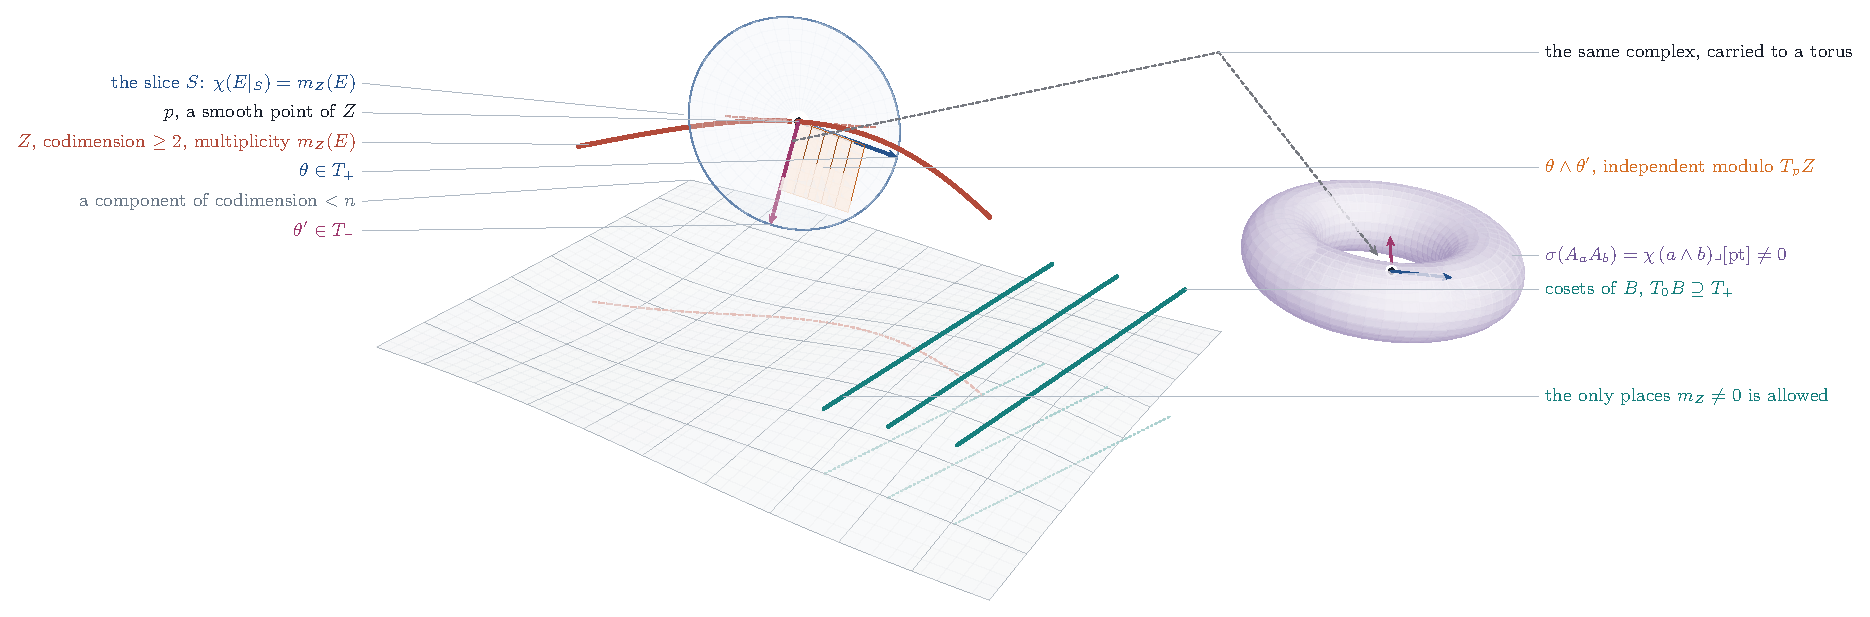
\includegraphics[width=\textwidth]{fig_support}
\caption{The proof of \Cref{thm:p2support}. The grey sheet stands for a
component of the support of codimension less than $n$, which the theorem
forces to exist; the clay curve $Z$ for a component of codimension at least
two. At a smooth point $p$ of $Z$ the directions $\theta\in T_{+}$ and
$\theta'\in T_{-}$ span the slice $S$, transverse to $Z$, on which $E$ restricts
to a complex of finite length with Euler characteristic $m_{Z}(E)$; the amber
parallelogram is the bivector $\theta\wedge\theta'$, independent modulo
$T_{p}Z$. Carried to a torus of the same dimension, the product of the two
jet classes is seen by the semiregularity map as $m_{Z}(E)$ times the class of
a point contracted with the bivector, which is not zero, so $m_{Z}(E)=0$ or
the bivector degenerates. The teal lines are cosets of an abelian subvariety
$B$ tangent to $T_{+}$, the only components of codimension at least two on
which a nonzero multiplicity survives. The scene is schematic in the
dimensions and exact in the incidences.}
\label{fig:support}
\end{figure}

\subsection{Indecomposability and endomorphisms}

The numerical criterion of \Cref{thm:p2numerical} fixes one number,
$\dim\Ext^{2}(E,E)$. Together with Serre duality, the lower bounds of
\Cref{cor:hhfactor} in the other degrees and the Hodge--Riemann relations for
the Weil class, it fixes a good deal more: the object that carries the class
can be taken indecomposable, and it has at least three linearly independent
endomorphisms at $n=2$ and, granting the compatibility of
\Cref{cor:hhfactor}(iii), at $n=3$, the first case in which the criterion
is needed at a nontrivial discriminant.

\begin{theorem}[The shape of an object meeting the criterion]
\label{thm:p2endo}
Let $A$, $\omega$ and $E$ be as in \Cref{thm:p2numerical}, so that
$\ch(E)=N\omega$ with $N\ne0$ and no other component, and suppose that
$\dim\Ext^{2}(E,E)=2n(2n-1)$. Write $e_{k}=\dim\Ext^{k}(E,E)$.
\begin{enumerate}[label=\textup{(\roman*)},leftmargin=2.6em,itemsep=2pt]
\item $\chi(E,E)=\sum_{k}(-1)^{k}e_{k}=(-1)^{n}N^{2}\int_{A}\omega^{2}$, and
  this number is positive.
\item $E\cong E_{0}\oplus E'$ with $E_{0}$ indecomposable,
  $\ch(E_{0})=\ch(E)$, $\dim\Ext^{2}(E_{0},E_{0})=2n(2n-1)$, $\ch(E')=0$ and
  $\Ext^{2}(E_{0},E')=\Ext^{2}(E',E_{0})=\Ext^{2}(E',E')=0$. So $E_{0}$ meets
  the criterion as well.
\item If $E$ is indecomposable, then $\End(E)=\CC\cdot\id\oplus J$ with $J$
  the nilpotent radical, every $f\in J$ annihilates $\Ext^{2}(E,E)$ and
  $\Ext^{2n-2}(E,E)$ under the Yoneda product, and
  $\operatorname{ev}_{E}(\bigwedge^{2n}P)=\operatorname{ev}_{E}(\bigwedge^{2n}Q)$
  is a single line in $\Ext^{2n}(E,E)$. If moreover $e_{1}=4n$, then $J$
  annihilates $\Ext^{1}(E,E)$ as well.
\item If $n=2$ or $n=3$, then
  \[
    \dim\End(E)\;\ge\;2+\tfrac12\,\chi(E,E)\;>\;2,
  \]
  so $E$ has at least three linearly independent endomorphisms, and at
  $n=3$ also $e_{1}\le e_{0}+9$. In particular no simple object meets the
  criterion: no stable sheaf, no complex with $\End=\CC$, and no image of one
  under an autoequivalence of $D^{b}(A)$; and an indecomposable object that
  meets it has a nonzero nilpotent endomorphism. The smallest profiles
  $(e_{0},\dots,e_{2n})$ that the constraints allow are $(3,8,12,8,3)$ at
  $n=2$, with $\chi=2$, and $(3,12,30,40,30,12,3)$ and $(3,12,30,41,30,12,3)$
  at $n=3$, with $\chi=2$ and $\chi=1$.
\end{enumerate}
Parts (i) and (ii), and part (iv) at $n=2$, use the compatibility
$\sigma_{E}\circ\operatorname{ev}_{E}=(\,\cdot\,)\lrcorner\ch(E)$ of
\Cref{setup:hh} in degree two only, as \Cref{thm:p2numerical} does. Part
(iii), and part (iv) at $n=3$, use it in the further degrees in which
\Cref{cor:hhfactor}(iii) grants it: $2n-2$ and $2n$ for (iii), and three for
(iv).
\end{theorem}

\begin{proof}
(i) The Todd class of $A$ is trivial, so the Riemann--Roch theorem gives
$\chi(E,E)=\int_{A}\ch(E)^{\vee}\ch(E)$, and $\ch(E)^{\vee}=(-1)^{n}N\omega$
since $\omega$ has degree $2n$. The polarisation pairs $V_{+}$ only with
$V_{-}$ (see \cite[Figure~9]{paperI}), so its class $\theta$ lies in
$V_{+}\otimes V_{-}$ and $\theta\wedge\alpha_{\pm}=0$, because $\alpha_{\pm}$
spans the top exterior power of $V_{\pm}$. So $\omega$ is a nonzero rational
primitive class of type $(n,n)$ in the middle degree, and the Hodge--Riemann
relations give $(-1)^{n(2n-1)}\int_{A}\omega^{2}>0$, where
$(-1)^{n(2n-1)}=(-1)^{n}$.

(ii) The category $D^{b}(A)$ has finite dimensional morphism spaces and split
idempotents, so $E=\bigoplus_{i}E_{i}$ with each $E_{i}$ indecomposable. The
evaluation map and the semiregularity map are compatible with direct sums,
and by \Cref{thm:p2numerical}(i) the kernel of $\operatorname{ev}_{E}$ in
degree two is $P\wedge Q$; so $\operatorname{ev}_{E_{i}}(P\wedge Q)=0$ and,
composing with $\sigma_{E_{i}}$, $(P\wedge Q)\lrcorner\ch(E_{i})=0$ for every
$i$. We claim that the only classes of Hodge type killed by $P\wedge Q$ are
those of $\CC\alpha_{+}\oplus\CC\alpha_{-}$. Write
$H^{*}(A,\CC)=\bigwedge^{*}(A_{+}\oplus B_{+}\oplus A_{-}\oplus B_{-})$ with
$A_{\pm}=V_{\pm}^{1,0}$ and $B_{\pm}=V_{\pm}^{0,1}$, and grade it by the four
degrees $(i,j,k,l)$. As in \Cref{setup:hh}, $P$ acts by wedging with $B_{+}$
and contracting $A_{-}$, and $Q$ by wedging with $B_{-}$ and contracting
$A_{+}$, so $P\wedge Q$ is spanned by four kinds of operators, each of which
shifts the four degrees by a fixed amount: wedging with $b_{+}\wedge b_{-}$
kills a component of degree $(i,j,k,l)$ for all choices exactly when $j=n$ or
$l=n$; wedging with $b_{+}$ after contracting $a_{+}$, exactly when $i=0$ or
$j=n$; contracting $a_{-}$ and wedging with $b_{-}$, exactly when $k=0$ or
$l=n$; and contracting $a_{-}$ and $a_{+}$, exactly when $i=0$ or $k=0$. Each
of these is a statement about a tensor product of maps that are injective
unless the degree in question is extreme. A class of type $(p,p)$ has
$i+k=j+l=p$ in every component. If $j=n$, then $l=n$ would force $i=k=n$,
against the fourth condition, so $l<n$ and the third condition gives $k=0$;
hence $i=n+l$, so $i=n$ and $l=0$: the component lies in
$\bigwedge^{n}A_{+}\otimes\bigwedge^{n}B_{+}=\CC\alpha_{+}$. If $j<n$, the
first two conditions give $l=n$ and $i=0$, hence $k=n$ and $j=0$: the
component lies in $\CC\alpha_{-}$. This proves the claim. Since $\ch(E_{i})$ is a rational class of
Hodge type killed by $P\wedge Q$, it lies on the rational Weil plane, and
when it is nonzero \Cref{cor:hhfactor}(i) gives
$\dim\Ext^{2}(E_{i},E_{i})\ge2n(2n-1)$, a nonzero rational Weil class having
both coefficients $a$ and $b$ nonzero. As
$\Ext^{2}(E,E)=\bigoplus_{i,j}\Ext^{2}(E_{i},E_{j})$ has dimension
$2n(2n-1)$ and $\sum_{i}\ch(E_{i})=N\omega\ne0$, exactly one summand $E_{0}$
has nonzero Chern character and every other block of $\Ext^{2}$ vanishes.

(iii) An indecomposable object of a category with finite dimensional
morphism spaces and split idempotents has a local endomorphism ring, so
$\End(E)=\CC\cdot\id\oplus J$ with $J$ nilpotent. By
\Cref{thm:p2numerical}(i), $\operatorname{ev}_{E}$ maps
$\bigwedge^{2}P\oplus\bigwedge^{2}Q$ isomorphically onto $\Ext^{2}(E,E)$.
By Serre duality $e_{2n-2}=e_{2}$, and contraction with $\omega$ is injective
on $\bigwedge^{2n-2}P\oplus\bigwedge^{2n-2}Q$ by \Cref{thm:hhsplitting}(iv),
since $2n-2\ne2n$; so, with the compatibility in
degree $2n-2$, $\operatorname{ev}_{E}$ maps that space isomorphically onto
$\Ext^{2n-2}(E,E)$. In degree $2n$ the semiregularity map is the trace, since
$H^{q+2n}(\Omega^{q}_{A})=0$ for $q>0$, so
$\operatorname{tr}\operatorname{ev}_{E}(\xi)$ is the $H^{0,2n}$ component of
$\xi\lrcorner\ch(E)$; for the generators $\pi_{P}$, $\pi_{Q}$ of
$\bigwedge^{2n}P$ and $\bigwedge^{2n}Q$ it is $Nc_{P}$ and $Nc_{Q}$ with
$c_{P}c_{Q}\ne0$. Indeed $\pi_{P}$ wedges with a basis of $B_{+}$ and contracts
a basis of $A_{-}$, so it kills $\alpha_{+}$, whose factor $\bigwedge^{n}B_{+}$
is already full, and carries $\alpha_{-}$ to $\pm$ the generator
$\bigwedge^{n}B_{+}\wedge\bigwedge^{n}B_{-}$ of $H^{0,2n}$; so $c_{P}=\pm b$
and likewise $c_{Q}=\pm a$, both nonzero. For $f\in\End(E)$ and
$x\in\bigwedge^{2}P\oplus\bigwedge^{2}Q$ write
$f\cdot\operatorname{ev}_{E}(x)=\operatorname{ev}_{E}(\varphi_{f}(x))$; then
$f\mapsto\varphi_{f}$ is a homomorphism of algebras. Let $x\in\bigwedge^{2}P$
and $y\in\bigwedge^{2n-2}P$, and write $x\wedge y=\beta(x,y)\pi_{P}$. Since
$\operatorname{ev}_{E}$ is a ring map that kills the ideal generated by
$P\wedge Q$,
\[
  \beta(x,y)\operatorname{tr}\bigl(f\operatorname{ev}_{E}(\pi_{P})\bigr)
  =\operatorname{tr}\bigl(f\operatorname{ev}_{E}(x)\operatorname{ev}_{E}(y)\bigr)
  =\operatorname{tr}\operatorname{ev}_{E}\bigl(\varphi_{f}(x)\wedge y\bigr)
  =Nc_{P}\,\beta\bigl(\varphi_{f}(x)_{P},y\bigr),
\]
and the pairing $\beta$ is perfect, so $\varphi_{f}(x)_{P}=\mu_{f}x$ with
$\mu_{f}=\operatorname{tr}(f\operatorname{ev}_{E}(\pi_{P}))/Nc_{P}$. The same
computation with $y\in\bigwedge^{2n-2}Q$, where $x\wedge y$ lies in the ideal
generated by $P\wedge Q$, gives $\varphi_{f}(x)_{Q}=0$. So $f$ acts on
$\operatorname{ev}_{E}(\bigwedge^{2}P)$ by a scalar $\mu_{f}$, and in the same
way on $\operatorname{ev}_{E}(\bigwedge^{2}Q)$ by a scalar $\nu_{f}$; $\mu$ and
$\nu$ are characters of $\End(E)$ and vanish on $J$. So $J$ kills
$\Ext^{2}(E,E)$, on both sides because $\operatorname{ev}_{E}$ lands in the
graded centre, and the same argument with the roles of the two degrees
exchanged shows that it kills $\Ext^{2n-2}(E,E)$. In particular
$\operatorname{tr}(f\operatorname{ev}_{E}(\pi_{P}))=\mu_{f}Nc_{P}=0$ for
$f\in J$, so $\operatorname{ev}_{E}(\pi_{P})$ and, likewise,
$\operatorname{ev}_{E}(\pi_{Q})$ lie in the annihilator of $J$ under the
perfect pairing of $\End(E)$ with $\Ext^{2n}(E,E)$. That annihilator is a
line, $J$ having codimension one, and both elements are nonzero, their traces
being $Nc_{P}$ and $Nc_{Q}$; so they span the same line. Finally, if
$e_{1}=4n$ then $\Ext^{1}(E,E)=\operatorname{ev}_{E}(HH^{1})$, because
$\operatorname{ev}_{E}$ is injective on $HH^{1}$, as shown in (iv). For
$f\in J$ and $h\in HH^{1}$ write $f\operatorname{ev}_{E}(h)=
\operatorname{ev}_{E}(h')$; then
$\operatorname{ev}_{E}(h'\wedge h'')=f\operatorname{ev}_{E}(h\wedge h'')=0$ for
every $h''\in HH^{1}$, so $h'\wedge HH^{1}\subseteq P\wedge Q$, which forces
$h'=0$ since $\dim P=\dim Q\ge2$.

(iv) By Serre duality $e_{k}=e_{2n-k}$. The map $\operatorname{ev}_{E}$ is
injective on $HH^{1}$ using degree two alone: if $\operatorname{ev}_{E}(h)=0$
then $\operatorname{ev}_{E}(h\wedge h')=0$ for every $h'$, so
$h\wedge HH^{1}\subseteq\Ann_{HH^{2}}(\omega)=P\wedge Q$, and $h=0$ as in
(iii). So $e_{1}\ge4n$, and \Cref{cor:hhfactor}(iii) gives
$e_{3}\ge2\binom{6}{3}=40$ at $n=3$. At $n=2$ the Euler
characteristic is $2e_{0}-2e_{1}+12$, and at $n=3$ it is
$2e_{0}-2e_{1}+60-e_{3}$. So $2e_{0}=\chi+2e_{1}-12\ge\chi+4$ at $n=2$, and
$2e_{0}=\chi+2e_{1}+e_{3}-60\ge\chi+4$ at $n=3$, where also
$e_{1}=e_{0}+30-\frac12(\chi+e_{3})\le e_{0}+9$. With (i) this gives the
bound. An autoequivalence preserves $\End$, and a stable sheaf is simple.
An indecomposable object with $\dim\End\ge3$ has $J\ne0$. For the smallest
profiles take $e_{0}=3$. At $n=2$, $\chi$ is even and positive, so
$2e_{1}=18-\chi\le16$, and $e_{1}\ge8$ forces $e_{1}=8$ and $\chi=2$. At
$n=3$, $2e_{1}+e_{3}=66-\chi\le65$ with $e_{1}\ge12$ and $e_{3}\ge40$
forces $e_{1}=12$ and $e_{3}\in\{40,41\}$, with $\chi=2$ and $\chi=1$.
\end{proof}

\begin{remark}[Objects excluded by the shape]\label{rem:p2endo}
\Cref{thm:p2endo} gives necessary conditions only, and their effect is to
exclude the objects one would construct first. Line bundles, semi-homogeneous
bundles, skyscraper sheaves, stable sheaves and their Fourier--Mukai
transforms are simple, and direct sums of them are excluded by (ii) together
with \cite[Theorem~2.32]{paperIII}. At $n=3$, granting the compatibility of
\Cref{cor:hhfactor}(iii), the shape allowed is an indecomposable object
with a local endomorphism algebra of dimension at least three whose radical
kills $\Ext^{2}$ and $\Ext^{4}$ and pairs to zero with the line
$\operatorname{ev}_{E}(\bigwedge^{6}P)$. The smallest conceivable one has
$\Hom(E,E)$ of dimension three, $\Ext^{1}(E,E)$ equal to the image of
$HH^{1}(A)$, of dimension twelve and killed by the radical, and
$\Ext^{3}(E,E)$ of dimension forty or forty-one. Iterated self-extensions and
thickenings are the natural objects with nilpotent endomorphisms, but an
extension of a simple object $F$ by itself has $\ch=2\ch(F)$, so $F$ would
already have to carry the class, and the question returns one level down.
For $n\ge4$ write $e_{k}=2\binom{2n}{k}+\delta_{k}$ for $1\le k\le2n-1$,
with $\delta_{k}\ge0$ and $\delta_{2}=\delta_{2n-2}=0$. Since
$\sum_{k=1}^{2n-1}(-1)^{k}\binom{2n}{k}=-2$, the Euler characteristic is
$2e_{0}-4+\sum_{k}(-1)^{k}\delta_{k}$, and an excess $\delta_{k}$ in an even
degree $4\le k\le2n-4$ can make it positive with $e_{0}=1$; so the bound on
$\End$ disappears. By
\Cref{thm:p2false} none of these shapes is realised.
\end{remark}
\section{The semiregularity criterion in its pure and polarised forms}\label{sec:polarised}

\subsection{Weil tori and the pure form of the criterion}

The object $E$ of \cite[Section~16]{paperI} has Chern character exactly
$N\omega$. For such an object, injectivity of $\sigma_{E}$ would make $E$
extend along every $K$-linear deformation of $A$ (\Cref{thm:p2forces}(ii)). These
deformations reach non-algebraic tori, on which the Weil class is a Hodge
class but not a Chern class of any coherent sheaf. This settles the pure form
of the criterion, negatively, in every dimension.

\begin{setupenv}[Weil tori]\label{setup:weiltori}
Let $A$ be an abelian $2n$-fold of $(K,-1,n)$-Weil type, $V=H^{1}(A,\QQ)$ with
its action of $K$, and $V\otimes\CC=V_{+}\oplus V_{-}$ the two eigenspaces,
each of dimension $2n$. For complementary $n$-dimensional subspaces
$X,Y\subset V_{+}$ the subspace $X\oplus\bbar{Y}$ of $V\otimes\CC$ is the
space of holomorphic $1$-forms of a complex structure on the real torus
underlying $A$; call the resulting complex torus $T_{X,Y}$. On $T_{X,Y}$ the
field $K$ acts with signature $(n,n)$, so $T_{X,Y}$ is a Weil torus in the
sense of \cite{Voi02b}, and every complex structure on that real torus
commuting with $K$ and of signature $(n,n)$ arises in this way. The pairs
$(X,Y)$ form a connected complex manifold $S$ of dimension $2n^{2}$,
containing the point of $A$; the polarised Weil family is the submanifold of
dimension $n^{2}$ on which the polarisation of $A$ is of type $(1,1)$, and the
tangent space of $S$ is the space $\Hom_{K}(H^{1,0},H^{0,1})$ of $K$-linear
first order deformations in \Cref{thm:p2forces}(i). Since
$\alpha_{+}$ spans $\bigwedge^{2n}V_{+}=\bigwedge^{n}X\otimes\bigwedge^{n}Y$
and $X$ is holomorphic while $Y$ is antiholomorphic, the Weil classes are of
type $(n,n)$ on every $T_{X,Y}$. We say that a property holds for a very
general member of $S$ if it holds outside a countable union of proper
analytic subsets.
\end{setupenv}

\begin{lemma}[The Hodge classes of a very general Weil torus]
\label{lem:weiltorushodge}
For a very general member $T$ of $S$, $\Hdg^{k}(T)=0$ for
$1\le k\le2n-1$, $k\ne n$, and $\Hdg^{n}(T)$ is the rational Weil plane.
\end{lemma}

\begin{proof}
There are countably many rational classes, and the Hodge locus of each is an
analytic subset of the connected manifold $S$; so a rational class that is of
Hodge type at a very general member is of Hodge type on all of $S$.
Let $G=\Res_{K/\QQ}\mathrm{GL}_{2n}$ be the group of $K$-linear automorphisms
of $V$. Its real points act transitively on $S$, since
$\mathrm{GL}(V_{+})$ acts transitively on pairs of complementary subspaces.
The Mumford--Tate group $M$ of a very general member lies in $G$, since $K$
acts by endomorphisms of every member, and it contains the Mumford--Tate group
of every member, whose Hodge classes include those of the very general one.
So the real Lie algebra of $M$ contains the complex structure $J_{s}$ of every
member, which is the derivative of its Hodge cocharacter, and therefore
contains the $\mathrm{Ad}\,G(\RR)$-span of one $J_{s}$. This span is an ideal of
$\mathfrak{g}_{\RR}=\mathfrak{gl}_{2n}(\CC)$ containing the non-central
element $J_{s}$, which acts on $V_{+}$ by $i$ on $X$ and by $-i$ on $Y$; hence
it contains $\mathfrak{sl}_{2n}(\CC)$, and $M$ contains
$G^{\mathrm{der}}=\Res_{K/\QQ}\mathrm{SL}_{2n}$. Over $\CC$ this is
$\mathrm{SL}(V_{+})\times\mathrm{SL}(V_{-})$ acting on
$\bigwedge^{*}(V_{+}\oplus V_{-})=\bigwedge^{*}V_{+}\otimes\bigwedge^{*}V_{-}$,
whose invariants are spanned by $1$, $\alpha_{+}$, $\alpha_{-}$ and
$\alpha_{+}\alpha_{-}$. Hodge classes are invariant under $M$, which gives
the statement.
\end{proof}

\begin{lemma}[A very general Weil torus has no subvarieties]
\label{lem:weiltorussubsets}
A very general member $T$ of $S$ has no analytic subsets other than finite
sets and $T$ itself.
\end{lemma}

\begin{proof}
Let $Z\subset T$ be an irreducible analytic subset of codimension $c$ with
$0<c<2n$. For every K\"ahler class $\kappa$ the class $[Z]$ satisfies
$\int_{T}[Z]\,\kappa^{2n-c}=\int_{Z}\kappa^{2n-c}>0$, so $[Z]$ is a nonzero
Hodge class of degree $2c$. By \Cref{lem:weiltorushodge} this forces $c=n$ and
$[Z]$ into the Weil plane. Take for $\kappa_{0}$ the class of a positive
definite hermitian form that is block diagonal for the splitting
$H^{1,0}=X\oplus\bbar{Y}$. Its blocks lie in $X\otimes\bbar{X}$ and
$\bbar{Y}\otimes Y$, both inside $V_{+}\otimes V_{-}$, so every power of
$\kappa_{0}$ has a factor from $V_{+}$ and a factor from $V_{-}$ in each term,
and $\alpha_{\pm}\wedge\kappa_{0}^{n}=0$ because $\alpha_{\pm}$ spans the top
exterior power of $V_{\pm}$. So
$\int_{T}[Z]\,\kappa_{0}^{n}=0$, which is impossible.
\end{proof}

\begin{proposition}[Coherent sheaves on a very general Weil torus]
\label{prop:weiltorussheaves}
Let $n\ge2$ and let $T$ be a very general member of $S$. Every coherent
analytic sheaf $F$ on $T$ has $\ch_{k}(F)=0$ in $H^{2k}(T,\QQ)$ for
$1\le k\le2n-1$. For $n=2$ this is Voisin's theorem that every coherent sheaf
on a general Weil torus of dimension four has $c_{2}(F)=0$
\cite[Theorem~10]{Voi02b}, whose proof we follow.
\end{proposition}

\begin{proof}
Chern classes of coherent sheaves on $T$ exist in rational Deligne
cohomology, extend those of bundles and are additive \cite{Gri10}, so they
are Hodge classes. By \Cref{lem:weiltorussubsets} the torsion of $F$, the locus where the
torsion-free quotient is not locally free, and the cokernel of the map from
that quotient to its reflexive hull are all supported on finite sets, and a
sheaf supported on a finite set has Chern character in the top degree only. So
it suffices to treat a reflexive sheaf $G$. Every coherent sheaf on $T$ has
$c_{1}=0$, since $\Hdg^{1}(T)=0$ (\Cref{lem:weiltorushodge}); so every
torsion-free sheaf has slope zero for every K\"ahler class, and a torsion-free
sheaf is stable for one K\"ahler class exactly when it has no saturated
subsheaf of intermediate rank, which does not depend on the class. A
Jordan--H\"older filtration of $G$ therefore has stable torsion-free factors
$Q_{j}$, stable for every K\"ahler class, and $\ch(G)=\sum_{j}\ch(Q_{j})$.
By the theorem of Bando and Siu \cite{BS94} the stable reflexive sheaf
$Q_{j}^{**}$ carries an admissible Hermite--Einstein metric for every K\"ahler
class $\kappa$ and satisfies
$\int_{T}\bigl(2rc_{2}-(r-1)c_{1}^{2}\bigr)(Q_{j}^{**})\,\kappa^{2n-2}\ge0$,
with equality exactly when $Q_{j}^{**}$ is a projectively flat vector bundle.
Here $c_{1}=0$ and $c_{2}(Q_{j}^{**})\in\Hdg^{2}(T)$. For $n\ge3$ that group is
zero; for $n=2$ it is the Weil plane, and then
$\int_{T}c_{2}(Q_{j}^{**})\,\kappa_{0}^{2}=0$ for the class $\kappa_{0}$ of
the proof of \Cref{lem:weiltorussubsets}. In either case equality holds for
some $\kappa$, so $Q_{j}^{**}$ is a projectively flat bundle with $c_{1}=0$,
hence flat, and its rational Chern classes of positive degree vanish. Since
$Q_{j}$ and $Q_{j}^{**}$ differ only on a finite set, $\ch_{k}(Q_{j})=0$ for
$1\le k\le2n-1$, and the same holds for $G$ and for $F$.
\end{proof}

\begin{theorem}[The pure form of the criterion is never met]
\label{thm:p2false}
Let $n\ge2$, let $A$ be an abelian $2n$-fold of $(K,-1,n)$-Weil type, $\omega$
a nonzero rational Weil class, and $E$ a perfect complex on $A$ with
$\ch(E)=N\omega$, $N\ne0$, and no other component. Then $\sigma_{E}$ is not
injective. In particular $\dim\Ext^{2}(E,E)>2n(2n-1)$, the hypotheses of
\Cref{thm:semiregclosure} and \Cref{thm:p2numerical}(iii) are satisfied by no
object at any member of any Weil family of an imaginary quadratic field, and
the propagation statement \textup{(P2)} of \Cref{rem:tworemain}, in the form
stated there, is false.
\end{theorem}

\begin{proof}
Suppose that $\sigma_{E}$ is injective. Since $A$ is projective, $E$ is isomorphic to
a bounded complex $E^{\bullet}$ of holomorphic vector bundles. The class
$N\omega$ is of Hodge type on every member of $S$ (\Cref{setup:weiltori}), so
by the theorem of Buchweitz and Flenner in Pridham's form (\Cref{thm:BF},
\cite{BF03,Pri24}), every obstruction to extending $E$ along an
Artinian deformation of $A$ inside $S$ vanishes, exactly as in the proof of
\Cref{thm:semiregclosure}. The deformations of the complex structure inside
$S$ together with those of the holomorphic structures and differentials of
$E^{\bullet}$ are governed by a differential graded Lie algebra of Dolbeault
type with finite dimensional cohomology, and Kuranishi's method
\cite{Kur65}, in the form of \cite[Sections~2--3]{GM88}, gives an analytic
germ $(M,m_{0})$ with a morphism $\pi\colon(M,m_{0})\to(S,s_{0})$ and a
complex of holomorphic vector bundles on the pulled back family of tori
deforming $E^{\bullet}$, whose completion is a hull of the formal deformation
functor. The vanishing of the obstructions says that $\pi$ is formally
smooth, hence smooth, so its image contains a neighbourhood $U$ of $s_{0}$.
Thus every member $T_{s}$ with $s\in U$ carries a bounded complex of
holomorphic vector bundles $E_{s}^{\bullet}$ whose Chern character is the
parallel transport of $N\omega$. Choose $s\in U$ very general. By
\Cref{prop:weiltorussheaves},
$\ch_{n}(E_{s})=\sum_{i}(-1)^{i}\ch_{n}(E_{s}^{i})=0$, while it is the
transport of $N\omega$, which is not zero. This contradiction proves that
$\sigma_{E}$ is not injective. The argument uses only that $\ch(E)$ is of
Hodge type on every member of $S$, so it applies verbatim when $\ch(E)-N\omega$
has components in degrees $0$ and $4n$ as well. The remaining statements
follow, since $\dim\Ext^{2}(E,E)\ge2n(2n-1)$ by \Cref{cor:hhfactor}(i),
and equality forces $\sigma_{E}$ to be injective by
\Cref{thm:p2numerical}(i).
\end{proof}

\begin{remark}[The polarised criterion]\label{rem:p2prime}
\Cref{thm:p2false} turns \Cref{thm:p2forces}(ii) from a constraint into a
contradiction: an object that extends along every $K$-linear deformation of
$A$ reaches non-algebraic tori, where the Weil class is a Hodge class but not
a Chern class. The results that describe such an object,
\Cref{thm:p2forces}, \Cref{cor:hhfactor}(ii)--(iii), \Cref{thm:p2numerical},
\Cref{thm:p2support}, \cite[Theorem~2.32]{paperIII} and \Cref{thm:p2endo}, remain true as
implications, but they are vacuous: no object satisfies their hypotheses.
They record what the pure form asks of an object, and
\Cref{rem:p2primesurvive} says which of them extend to the polarised form
defined next.

The obstruction does not reach a Chern character with a component that is of
Hodge type on the polarised family and not beyond it, unless a twist removes
that component. Call
\textup{(P2$'$)} the statement that at one base point of each Weil family
some perfect complex $E$ with
\[
  \ch(E)=N\omega_{1}+\sum_{k}c_{k}\,\theta^{k},\qquad N\ne0,\ c_{k}\in\QQ,
\]
$\theta$ the polarisation, has injective semiregularity map. The proof of
\Cref{thm:semiregclosure} applies to it word for word, with the deformation
taken over the polarised family, along which $\ch(E)$ stays of Hodge type:
at a member $A_{s}$ it produces $\ch_{n}(E_{s})=N\omega_{1}+c_{n}\theta^{n}$
algebraic, and $\theta^{n}$ is algebraic, so $\omega_{1}$ is. The form above
is already the most general one allowed by the subring generated by $\theta$
and the Weil classes: a Weil class is primitive, so $\theta\omega_{1}=0$ and
that subring is spanned by the powers of $\theta$ and the Weil plane.
\Cref{thm:p2false} excludes directly a Chern character that remains of Hodge
type on all of $S$, which by \Cref{lem:weiltorushodge} is a multiple of the
Weil class plus terms in degrees $0$ and $4n$, and after a line bundle twist
the characters $c\,e^{t\theta}+N\omega_{1}+c'\theta^{2n}$ with $t\theta$
integral (\Cref{thm:p2primenumber}(v)). For every other polarised character
with some $c_{k}\ne0$, $1\le k\le2n-1$, the component of the Hodge locus of
$\ch(E)$ through $A$ is the polarised family itself, whose members are
abelian varieties, so nothing forces $E$ onto non-algebraic tori and the
argument cannot be run on $E$ (\Cref{prop:p2primelocus}); the one exception is
a ratio at $n=2$ at which the locus is five-dimensional
(\Cref{rem:p2primeexceptional}). The semiregular objects in Markman's
proofs for abelian fourfolds and for the sixfolds of trivial discriminant
\cite{Mar25a,Mar25b} are not of the pure form: their Chern characters are not
multiples of a Weil class, and they are deformed only along families on which
those characters stay of Hodge type, and nothing below depends on whether
they have exactly the form above. From here on, in
\cite[Corollary~2.71]{paperIII}, \cite[Theorem~2.70]{paperIII} and the frontier of
\cite[Section~2]{paperIII}, \textup{(P2)} is read in this polarised form. The
annihilator computations of \cite[Section~16]{paperI} assume that $\ch(E)$ is a
pure Weil class; the next subsection carries them out for a Chern character
with components in every even degree (\Cref{thm:p2primenumber},
\Cref{prop:p2primeprofile}, \Cref{prop:p2primelocus}).

The same obstruction does not reach the Mumford target of
\cite[Section~3.2]{paperIII}. The exceptional classes there are rigid: their Hodge
locus among all complex tori is the Mumford curve (\cite[Theorem~3.21]{paperIII},
\cite[Proposition~3.24]{paperIII}), so a semiregular complex with Chern character
$N\omega$ on the square of a Mumford fourfold would only have to deform along
the curve, whose members are all algebraic.
\end{remark}

\begin{remark}[Two finite statements]
\label{rem:tworemain}
After \cite[Theorem~16.9]{paperI} and \Cref{thm:semiregclosure} the Hodge
conjecture for abelian varieties of Weil type follows from either of the
following, each of which is a statement about explicit finite data and neither
of which mentions a general point. The first is settled by
\cite[Theorem~16.17]{paperI}, and we record it because it is the form in which the
question first presents itself. The second is false as stated here
(\Cref{thm:p2false}), and its polarised form, \textup{(P2$'$)} of
\Cref{rem:p2prime}, is computed in closed form below.

\begin{enumerate}[label=\textup{(P\arabic*)},leftmargin=*]
\item \emph{A bound.} At every point of the orbit $G(\QQ)\cdot s_{0}$ the
  class $\omega$ is represented by a cycle whose Hilbert data comes from one
  finite set. \cite[Theorem~16.15]{paperI} shows that the transport of the base cycle
  does not satisfy this, for any cycle whose components have finite
  stabiliser, and \cite[Theorem~16.17]{paperI} shows that, read on an arbitrary
  representative, the statement is equivalent to $\mathbf{W}(K,n,\delta)$
  itself. It is therefore a reformulation of the conjecture for the family,
  and we record it as such rather than as a criterion.
\item \emph{A rank.} The semiregularity map of a perfect complex with the
  Chern character of \Cref{prop:ktheory} at one base point is injective.
  In this form the statement is false (\Cref{thm:p2false}); its polarised
  form, in \Cref{rem:p2prime}, allows the Chern character to carry powers of
  the polarisation, and what follows records what the pure form asks. The
  source of the map is $\Ext^{2}(E,E)$ for a single object, and its target
  has dimension $\sum_{q}h^{q,q+2}(A_{0})=\binom{4n}{2n-2}$, computed in
  \cite[Proposition~9.2]{paperI}. So the target is large, which is the direction that
  helps, and the question is the rank of the map. Full rank would force the
  following (\Cref{thm:p2forces}): the evaluation map of
  Hochschild cohomology must vanish on the $4n^{2}$-dimensional annihilator of
  the Weil class, so $E$ must be killed by the mixed block of $H^{0,2}$, must
  extend along every $K$-linear deformation, must have all products of
  transverse translation classes zero, and must have no endomorphism of
  nonzero trace; and at a base point with no abelian subvariety tangent to an
  eigenspace it can be a locally free sheaf on no smooth germ of its support
  of codimension at least two (\Cref{cor:p2shape}). The representative that
  the construction supplies, a virtual sum of line bundles, fails at the first
  of these (\cite[Proposition~9.10]{paperI}), and any representative that is a
  sheaf fails at the last. \Cref{thm:hhsplitting} identifies that
  annihilator as the mixed part of a splitting $HH^{1}=P\oplus Q$ into the
  annihilators of the two conjugate pieces of the class, and
  \Cref{cor:hhfactor} draws the consequence: the whole Hochschild action of
  $E$ factors through a ring of dimension $2^{2n+1}-1$ inside one of
  dimension $2^{4n}$, while $\dim\Ext^{2}(E,E)\ge2n(2n-1)$ for every
  representative, semiregular or not. \Cref{thm:p2numerical} turns the rank
  condition into that number: equality suffices. \Cref{thm:p2support} locates
  the support: at every member it has a component of codimension less than
  $n$, so no complex carried by a cycle representing $\omega$ can serve, and
  at a general member every component of codimension at least two has
  multiplicity zero.
  \Cref{thm:p2endo} fixes its shape: an indecomposable summand carries the
  class and meets the criterion alone, and at $n=2$, and at $n=3$ granting
  the compatibility of \Cref{cor:hhfactor}(iii), it has at least three
  independent endomorphisms, so no simple object serves.
\end{enumerate}

Neither statement is the variational Hodge conjecture: (P1) says nothing
about deformations, and (P2) is an infinitesimal statement at one point, the
global propagation being supplied by \cite[Theorem~16.4]{paperI}, which is what
\cite[Remark~B.11]{paperI} identifies as missing. Nor is either implied by the
results of \cite[Section~15.5]{paperI}: the base points and the cycles are
constructed there, and (P1) and (P2) are questions about those same cycles
that the construction does not answer. In the forms stated here both are
settled: (P1) is equivalent to its conclusion, and (P2) is false. Its
polarised form in \Cref{rem:p2prime} is the criterion that the rest of this
section computes.
\end{remark}

\subsection{The polarised criterion in closed form}

The annihilator computations of \cite[Section~16]{paperI} assume that $\ch(E)$
is a pure Weil class, as \Cref{rem:p2prime} notes. This subsection carries
them out for a Chern character with components in every even degree. In
degree two the answer is complete and holds for every $n$; in the other
degrees it is a closed formula, with one correction term in the middle
degree. The same computation gives the Hodge locus of the character,
and with it the list of the obstructions of this paper that apply to
polarised characters (\Cref{prop:p2primelocus}, \Cref{rem:p2primesurvive}).
None of this constructs an object or decides whether one exists. It gives,
for each shape of Chern character, the number that $\dim\Ext^{2}(E,E)$ has
to reach and the exact kernel that $\operatorname{ev}_{E}$ must then have,
which is the form in which a candidate can be tested.

\begin{setupenv}[Polarised characters]\label{setup:p2prime}
Let $A$ be an abelian $2n$-fold of $(K,-1,n)$-Weil type, $n\ge2$, with
polarisation $\theta$, and let $\omega=u\alpha_{+}+\bbar u\,\alpha_{-}$ be a
nonzero real class on the Weil line, in the notation of \Cref{thm:p2forces}.
For complex numbers $c_{0},\dots,c_{2n}$ put
\[
  p(\theta)=\sum_{k=0}^{2n}c_{k}\theta^{k},\qquad
  \gamma=\omega+p(\theta),\qquad \mu_{m}=m!\,c_{m},
\]
and let $\rho\in\{0,1,2,3\}$ be the rank of the $(2n-1)\times3$ Hankel matrix
$H=[\mu_{j+i}]$, $0\le j\le2n-2$, $0\le i\le2$. Write $r(\gamma)$ for the
rank of contraction $HT^{2}(A)\to H^{*}(A,\CC)$, $\xi\mapsto\xi\lrcorner\gamma$.
For $a<n\le b$, in the basis of \Cref{thm:hhsplitting} adapted to an
eigenbasis $e_{j}$ of $V_{+}$ and $f_{j}$ of $V_{-}$ with $e_{j},f_{j}$ of
type $(1,0)$ for $j<n$ and $j\ge n$ respectively, write
$z_{ab}=w(e_{b})w(f_{a})\in V_{+}^{0,1}\otimes V_{-}^{0,1}$,
$v^{1}_{ab}=w(e_{b})c(e_{a})$ and $v^{2}_{ab}=w(f_{a})c(f_{b})$ in
$H^{1}(T_{A})$, and $\pi_{ab}=c(e_{a})c(f_{b})\in T_{+}\otimes T_{-}$, where
$w$ is wedge product with a $(0,1)$ class and $c$ contraction of a $(1,0)$
class.
\end{setupenv}

The matrix $H$ is a catalecticant of the moment sequence
$\mu_{m}=m!\,c_{m}$. A nonzero vector $(x,\lambda,w)$ in its kernel is a
linear recurrence $x\mu_{j}+\lambda\mu_{j+1}+w\mu_{j+2}=0$ of order at most
two, so $\rho\le2$ says that the moments satisfy one, and the shapes of
\Cref{thm:p2primenumber}(ii) are its solutions, read off from the roots of
$wT^{2}+\lambda T+x$. For a Chern character,
$\gamma=N\omega_{1}+\sum_{k}c_{k}\theta^{k}$ with rational $c_{k}$, and $u$
is determined by $N\omega_{1}$. Since $\alpha_{\pm}^{2}=0$,
$\int_{A}\omega^{2}=2|u|^{2}\int_{A}\alpha_{+}\alpha_{-}$; scaling the
eigenbases so that $\int_{A}\alpha_{+}\alpha_{-}=(-1)^{n}\int_{A}\theta^{2n}/(2n)!$,
which is possible because the sign of $\int_{A}\alpha_{+}\alpha_{-}$ is
$(-1)^{n}$ by the Hodge--Riemann relations, one has
$|u|^{2}=(-1)^{n}\tfrac{(2n)!}{2}\int_{A}\omega^{2}\big/\!\int_{A}\theta^{2n}$.
The rank
$\rho$ does not change when
$\gamma$ is multiplied by $e^{t\theta}$, which acts on the moments by a
binomial transform, and $\omega e^{t\theta}=\omega$ because a Weil class is
primitive; so $\rho$ is an invariant of $\gamma$ up to twist.

\begin{theorem}[The polarised criterion as a number]\label{thm:p2primenumber}
In \Cref{setup:p2prime}:
\begin{enumerate}[label=\textup{(\roman*)},leftmargin=2.6em,itemsep=2pt]
\item For $n\ge3$,
  \[
    \Ann_{HT^{2}}(\gamma)=\bigoplus_{a<n\le b}
    \bigl\{x\,z_{ab}+y_{1}v^{1}_{ab}+y_{2}v^{2}_{ab}+w\,\pi_{ab}\;:\;
      (x,\;i(y_{1}-y_{2}),\;w)\in\ker H\bigr\},
  \]
  so that $\dim\Ann_{HT^{2}}(\gamma)=n^{2}(4-\rho)$ and
  $r(\gamma)=(4+\rho)n^{2}-2n$, whatever $u\ne0$ is.
\item $\rho=3$ for a general $p$. If $\rho=3$, and either $n\ge3$ or $n=2$ and
  $e=0$ in the notation of (iii), then $\Ann_{HT^{2}}(\gamma)$ is exactly
  the tangent space $T_{[A]}\cD_{n,n}$ of the polarised Weil family, spanned
  by the $n^{2}$ vectors $v^{1}_{ab}+v^{2}_{ab}$, inside $H^{1}(T_{A})$, with
  no component in $H^{0,2}$ or in $H^{0}(\bigwedge^{2}T_{A})$; and
  $r(\gamma)=\binom{4n}{2}-n^{2}=7n^{2}-2n$. Moreover $\rho\le2$ exactly when
  $p$ is one of $Ae^{s\theta}+Be^{t\theta}$, $(A+B\theta)e^{t\theta}$,
  $Ae^{t\theta}+B\theta^{2n}$, $A\theta^{2n-1}+B\theta^{2n}$, and $\rho\le1$
  exactly when $p\in\CC e^{t\theta}\cup\CC\theta^{2n}$; the pure case
  $\rho=0$ gives back $r=2n(2n-1)$ of \Cref{cor:hhfactor}(i).
\item For $n=2$, $\dim\Ann_{HT^{2}}(\gamma)=4(4-\rho)+e$ with
  $e=\dim\ker\bigl((HK)^{2}-|u|^{2}\bigr)\le2$ and $K$ the antidiagonal
  matrix with entries $1,-2,1$; so $r(\gamma)\in\{12,16,18,20,22,23,24\}$,
  and $e>0$ exactly when $X(X-I)^{2}=4J^{2}$, where $X=|u|^{2}$ and $I$, $J$
  are the two invariants of the binary quartic
  $\sum_{m}\binom{4}{m}\mu_{m}x^{4-m}y^{m}$.
\item Let $E$ be a perfect complex on $A$ with $\ch(E)=\gamma$ and $N\ne0$.
  Then $\dim\Ext^{2}(E,E)\ge r(\gamma)$ with no hypothesis on $\sigma_{E}$.
  If equality holds, then $\operatorname{ev}_{E}$ is onto with kernel
  $\Ann_{HT^{2}}(\gamma)$ and $\sigma_{E}$ is injective, so that
  \textup{(P2$'$)} holds at that point and, by \Cref{rem:p2prime} and
  \Cref{thm:semiregclosure}, the Hodge conjecture holds for every member of
  the family with full Hodge group. Conversely, if $\sigma_{E}$ is injective
  then $\ker\operatorname{ev}_{E}=\Ann_{HT^{2}}(\gamma)$.
\item If $p\in\CC e^{t\theta}+\CC\theta^{2n}$ with $t\theta$ the class of a line
  bundle $L$, a set of shapes with $\rho\le2$ that contains
  $\CC\theta^{2n}$, then no perfect complex $E$ with $\ch(E)=\gamma$ has
  injective $\sigma_{E}$.
\end{enumerate}
\end{theorem}

\begin{proof}
(i) Let the torus $(\CC^{\times})^{2n}$ act by $e_{j}\mapsto\tau_{j}e_{j}$,
$f_{j}\mapsto\tau_{j}^{-1}f_{j}$. It preserves the Hodge decomposition and
$\theta$, and scales $\alpha_{\pm}$ by $(\prod_{j}\tau_{j})^{\pm1}$;
contraction is equivariant. A weight of $HT^{2}$ has at most two nonzero
coordinates, so for $n\ge3$ two such weights never differ by a nonzero
multiple of $(1,\dots,1)$, and the images of one weight component in the
$\theta$-part and in the two $\alpha$-parts land in distinct weight spaces.
Hence $\Ann(\gamma)=\Ann(p(\theta))\cap\Ann(\alpha_{+})\cap\Ann(\alpha_{-})$,
and the last two meet in $P\wedge Q$ by \Cref{thm:hhsplitting}(ii). The space
$P\wedge Q$ is the sum over $a<n\le b$ of the four-dimensional weight spaces
spanned by $z_{ab},v^{1}_{ab},v^{2}_{ab},\pi_{ab}$, and $\Ann(p(\theta))$ is
torus-stable, so the computation splits pair by pair. Put
$m=e_{b}\wedge f_{a}$ and $\theta'=\theta-t_{a}-t_{b}$, where
$t_{j}=i s_{j}e_{j}\wedge f_{j}$ with $s_{j}=\pm1$ the sign that makes
$\theta=\sum_{j}t_{j}$ positive. Since the $t_{j}$ are even with
$t_{j}^{2}=0$, direct evaluation gives
\[
  z\lrcorner\theta^{k}=m\,\theta'^{k},\quad
  v^{1}\lrcorner\theta^{k}=ik\,m\,\theta'^{k-1},\quad
  v^{2}\lrcorner\theta^{k}=-ik\,m\,\theta'^{k-1},\quad
  \pi\lrcorner\theta^{k}=k(k-1)\,m\,\theta'^{k-2},
\]
so for $\xi=xz+y_{1}v^{1}+y_{2}v^{2}+w\pi$ and $\lambda=i(y_{1}-y_{2})$,
\[
  \xi\lrcorner p(\theta)=m\wedge\sum_{j=0}^{2n-2}\frac{\theta'^{j}}{j!}
  \bigl(x\mu_{j}+\lambda\mu_{j+1}+w\mu_{j+2}\bigr).
\]
The classes $m\wedge\theta'^{j}$, $0\le j\le2n-2$, are nonzero and of distinct
degrees, so $\xi$ kills $p(\theta)$ exactly when $(x,\lambda,w)\in\ker H$.
The map $(x,y_{1},y_{2},w)\mapsto(x,\lambda,w)$ is onto with kernel spanned by
$v^{1}+v^{2}$, which gives $1+(3-\rho)$ dimensions for each of the $n^{2}$
pairs. (ii) The vector $v^{1}_{ab}+v^{2}_{ab}$ is $K$-linear and kills
$\theta$, and these $n^{2}$ vectors span the tangent space of the polarised
family by \cite[Proposition~9.14]{paperI}; when $\rho=3$ they are all of the
annihilator. If $\rho\le2$, a nonzero $(x,\lambda,w)\in\ker H$ turns the
equations $x\mu_{j}+\lambda\mu_{j+1}+w\mu_{j+2}=0$ into a linear recurrence of
full rank on $\mu_{0},\dots,\mu_{2n}$, whose two-dimensional space of
solutions is spanned by the listed shapes according to the roots of
$wT^{2}+\lambda T+x$; $\rho\le1$ is the intersection of two such spaces.
(iii) At $n=2$ the argument of (i) fails for exactly one pair of weights,
$\epsilon_{2}+\epsilon_{3}$ in $\bigwedge^{2}P$ and $-\epsilon_{0}-\epsilon_{1}$
in $\bigwedge^{2}Q$, whose difference is $(1,1,1,1)$; these give one coupled
block of size eight, whose kernel is isomorphic to $\ker(X-T)$ with $T$
conjugate on its image to $(HK)^{2}$, and the characteristic polynomial of
$HK$ is $y^{3}-Iy-2J$, which is traceless, so $e\le2$. (iv) is the argument of
\Cref{thm:p2numerical}(i)--(ii) with $\Ann_{HT^{2}}(\gamma)$ in place of
$P\wedge Q$: $\sigma_{E}\circ\operatorname{ev}_{E}$ is contraction into
$\gamma$, so $\ker\operatorname{ev}_{E}\subseteq\Ann_{HT^{2}}(\gamma)$. (v) If
$\gamma-\omega$ has components in degrees $0$ and $4n$ only, the proof of
\Cref{thm:p2false} applies verbatim. If $p=c\,e^{t\theta}+c'\theta^{2n}$ with
$t\theta=c_{1}(L)$, then
$\ch(E\otimes L^{-1})=\gamma e^{-t\theta}=c+\omega+c'\theta^{2n}$, because
$\omega\theta=0$ and $\theta^{2n+1}=0$, and
$\sigma_{E\otimes L^{-1}}=e^{-c_{1}(L)}\cdot\sigma_{E}$ is injective exactly
when $\sigma_{E}$ is, so the first case applies to $E\otimes L^{-1}$.
\end{proof}

For a general shape, then, the polarised criterion asks of one complex that
$\dim\Ext^{2}(E,E)$ be $24$ at $n=2$, $57$ at $n=3$ and $104$ at $n=4$,
against $12$, $30$ and $56$ for the pure form, and injectivity then forces
nothing beyond first-order extension along the polarised family, which is
what the criterion is for. The larger number comes from the components
$c_{k}\theta^{k}$: every direction of $HT^{2}$ other than the $n^{2}$
directions of the family moves $\gamma$ off the Hodge classes, so an object
meeting the bound has $\operatorname{ev}_{E}$ injective on a complement of
$T_{[A]}\cD_{n,n}$. \Cref{fig:hankel} plots the number against $n$ for the
four Hankel ranks.

\begin{figure}[tbp]
\centering
  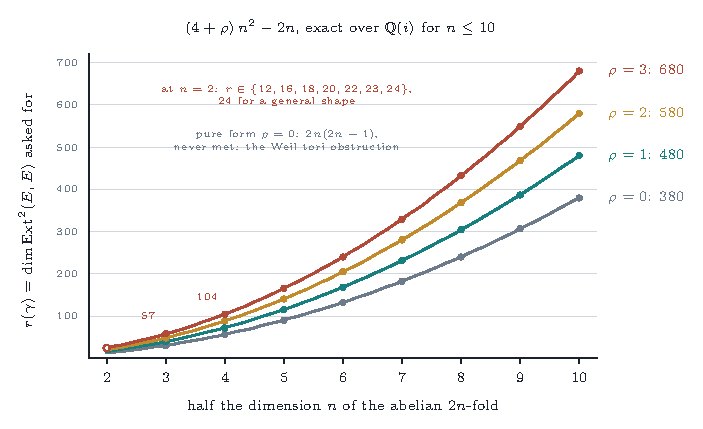
\includegraphics[width=0.86\textwidth]{fig_hankel}
\caption{The dimension $r(\gamma)=(4+\rho)n^{2}-2n$ that
$\Ext^{2}(E,E)$ must have for a complex with Chern character
$\gamma=N\omega_{1}+\sum_{k}c_{k}\theta^{k}$ to meet the polarised criterion,
for the four Hankel ranks $\rho$ of \Cref{thm:p2primenumber}; the dots mark
the values at $n=2,\dots,10$, and at $n=10$ the space $HT^{2}$ has dimension
$780$. The pure form, $\rho=0$, is the bottom curve
$2n(2n-1)$, which no complex attains (\Cref{thm:p2false}); a general shape
lies on the top curve $7n^{2}-2n$. At $n=2$ the weight argument fails for one
pair of weights and seven values occur.}
\label{fig:hankel}
\end{figure}

\begin{proposition}[The Hochschild profile of a polarised character]
\label{prop:p2primeprofile}
In \Cref{setup:p2prime}, let $\rho_{k}$ be the rank of contraction
$HT^{k}(A)\to H^{*}(A,\CC)$ into $\gamma$, put $C_{l}=l!\,c_{l}$, let
$r'$ be the rank of the $(n+1)\times(n+1)$ Hankel matrix $H'=[C_{p+q}]$, and
$d=\dim\ker\bigl((K'H')^{2}-|u|^{2}\bigr)$ with
$K'=\mathrm{antidiag}\bigl((-1)^{a}\binom{n}{a}\bigr)$.
\begin{enumerate}[label=\textup{(\roman*)},leftmargin=2.6em,itemsep=2pt]
\item $\rho_{0}=\rho_{2n}=1$, $\rho_{k}=0$ for $k>2n$, and for
  $1\le k\le2n-1$, $k\ne n$,
  \[
    \rho_{k}=2\binom{2n}{k}+M_{k}\min(k+1,\,2n+1-k,\,r'),\qquad
    M_{k}=\sum_{\substack{i+j=k\\1\le i,j\le n-1}}\binom{n}{i}\binom{n}{j};
  \]
  in the middle degree the same formula holds with $d$ subtracted. In particular $\rho_{k}=\rho_{2n-k}$, and the general
  profiles are $(1,8,24,8,1)$ at $n=2$ and $(1,12,57,112,57,12,1)$ at
  $n=3$.
\item $\chi(E,E)=V\,Q(c)+W$ for a perfect complex with $\ch(E)=\gamma$, where
  $V=\int_{A}\theta^{2n}>0$, $W=(-1)^{n}\int_{A}\omega^{2}>0$ and
  $Q(c)=\sum_{k}(-1)^{k}c_{k}c_{2n-k}$; and $\chi(E,E)$ is even.
\item Granting the compatibility of \Cref{cor:hhfactor}(iii) in every degree,
  $\dim\Ext^{k}(E,E)\ge\rho_{k}$. At $n=2$, at the points with $d=1$ one has
  $\rho_{2}=23$, which is odd, so $\dim\Ext^{2}(E,E)=r(\gamma)$ cannot hold
  there, since $\chi(E,E)$ is even and Serre duality gives
  $\chi(E,E)\equiv\dim\Ext^{2}(E,E)\bmod2$.
\end{enumerate}
\end{proposition}

\begin{proof}
(i) Split $HT^{1}=Q\oplus P$ as in \Cref{thm:hhsplitting}, so that
$HT^{k}=\bigoplus_{i+j=k}\bigwedge^{i}Q\otimes\bigwedge^{j}P$ and $Q$, $P$ act
on the two tensor factors of $H^{*}(A)=H_{+}\otimes H_{-}$ separately. A mixed
monomial kills $\omega$, and on $p(\theta)$ the block of mixed monomials with
fixed index sets $I$, $J$ has entries $C_{s+t+m+m'}$ depending only on
$s+t$ and $m+m'$, so its rank is that of a catalecticant of the binary form
$\sum_{k}c_{k}x^{k}y^{2n-k}/(2n-k)!$, which is $\min(k+1,2n+1-k,r')$ by the
classical Hilbert function of an apolar ideal. The pure sources
$\bigwedge^{k}Q$ and $\bigwedge^{k}P$ kill $\alpha_{-}$ and $\alpha_{+}$
respectively and contract the other class injectively
(\Cref{thm:hhsplitting}(iii)). To see where their images go, use the torus of
the proof of \Cref{thm:p2primenumber}(i) and put $I_{Q}=\{j<n\}$,
$I_{P}=\{j\ge n\}$. The basis vectors $w(f_{j}),c(e_{j})$ of $Q$ have weight
$-\epsilon_{j}$ for $j\in I_{Q}$, the vectors $w(e_{j}),c(f_{j})$ of $P$ have
weight $\epsilon_{j}$ for $j\in I_{P}$, $\theta$ has weight $0$ and
$\alpha_{\pm}$ has weight $\pm\sum_{j}\epsilon_{j}$. If $\xi\in\bigwedge^{k}Q$
is a monomial, $k<2n$, and another monomial $\eta$ of $HT^{k}$ sends
$p(\theta)$ or $\alpha_{-}$ to the weight of $\xi\lrcorner\alpha_{+}$, which is
$+1$ at every $j\in I_{P}$, then it is not $\alpha_{-}$, which would need two
factors from $P$ at every $j\in I_{P}$; so $\eta$ has one factor from $P$ for
each $j\in I_{P}$, $\xi$ has weight at most $-1$ at every $j\in I_{Q}$, and
$k\ge n$. For $k=n$ this forces $\xi$ and $\eta$ to lie in the spans
$D_{Q}\subset\bigwedge^{n}Q$ and $D_{P}\subset\bigwedge^{n}P$ of the $2^{n}$
monomials with one factor for each index. The same holds with $P$ and $Q$
exchanged. A mixed monomial kills
$\omega$, so for $k<n$ the matrix of contraction is block triangular, the pure
blocks injective onto targets of their own, and $\rho_{k}$ is $2\binom{2n}{k}$
plus the rank of the mixed blocks; for $k>n$ the formula follows from
\cite[Lemma~3.33]{paperIII}, which also gives $\rho_{k}=\rho_{2n-k}$.

For $k=n$, a pure monomial outside $D_{Q}\cup D_{P}$ repeats an index, so it
kills $1$ and $t_{j}$ at that index and hence $p(\theta)$, and keeps a target
of its own; no mixed monomial reaches the weights $\sum_{j\in I_{P}}
\epsilon_{j}$ and $-\sum_{j\in I_{Q}}\epsilon_{j}$ of the images of
$D_{Q}\oplus D_{P}$, since it would need $n$ factors from one side. So
$\rho_{n}$ is the value of the formula minus the dimension of the kernel of the
block $\beta\colon D_{Q}\oplus D_{P}\to T_{1}\oplus T_{2}$, $T_{1}$ and $T_{2}$
being the targets of those two weights. For $R\subseteq I_{Q}$ and
$J\subseteq I_{P}$ let $X_{R}=\prod_{j\in I_{Q}}z_{j}$ with $z_{j}=w(f_{j})$ for
$j\in R$ and $c(e_{j})$ otherwise, and $Y_{J}=\prod_{j\in I_{P}}z_{j}$ with
$z_{j}=c(f_{j})$ for $j\in J$ and $w(e_{j})$ otherwise, the factor of largest
index acting first, and write $\alpha_{+}=a\,e_{0}\cdots e_{2n-1}$,
$\alpha_{-}=b\,f_{0}\cdots f_{2n-1}$. Since
$\theta^{2n}/(2n)!=\prod_{j}t_{j}=\prod_{j}s_{j}\,e_{0}\cdots e_{2n-1}
f_{0}\cdots f_{2n-1}$, the normalisation of \Cref{setup:p2prime} gives
$ab=(-1)^{n}\prod_{j}s_{j}$. As the $t_{j}$ are even with $t_{j}^{2}=0$,
$p(\theta)=\sum_{S}\mu_{|S|}\prod_{j\in S}t_{j}$. Each operator acts on one
factor of $H^{*}(A)=\bigotimes_{j}\bigwedge^{*}\langle e_{j},f_{j}\rangle$
with the Koszul sign of the factors before it, and in each of the four
products below the parities of those factors do not depend on $R$ or $J$;
the signs are $+1$ on $p(\theta)$, $\epsilon_{1}=(-1)^{n(n-1)/2}$ for $X_{R}$ on
$\alpha_{+}$ and $\epsilon_{2}=(-1)^{n(3n-1)/2}$ for $Y_{J}$ on $\alpha_{-}$.
With $\tau_{R}=e_{n}\cdots e_{2n-1}\prod_{j\in R}t_{j}$ and
$\tau'_{R'}=f_{0}\cdots f_{n-1}\prod_{j\in R'}t_{j}$, and using
$c(f_{j})t_{j}=-is_{j}e_{j}$, $c(e_{j})t_{j}=is_{j}f_{j}$ and
$e_{j}f_{j}=-is_{j}t_{j}$, one finds
\begin{align*}
  X_{R}\lrcorner\,\alpha_{+}&=\epsilon_{1}a\prod_{j\in R}(is_{j})\,\tau_{R},&
  Y_{J}\lrcorner\,p(\theta)&=\sum_{R}\mu_{|J|+|R|}\prod_{j\in J}(-is_{j})\,\tau_{R},\\
  Y_{J}\lrcorner\,\alpha_{-}&=\epsilon_{2}b\prod_{j\in I_{P}\setminus J}(-is_{j})\,
    \tau'_{I_{P}\setminus J},&
  X_{R}\lrcorner\,p(\theta)&=\sum_{R'}\mu_{n-|R|+|R'|}\prod_{j\in I_{Q}\setminus R}
    (is_{j})\,\tau'_{R'}.
\end{align*}
For $x=\sum_{R}x_{R}X_{R}$ and $y=\sum_{J}y_{J}Y_{J}$ put
$\tilde x_{R}=\prod_{j\in R}(is_{j})\,x_{R}$ and
$\tilde y_{J}=\prod_{j\in J}(-is_{j})\,y_{J}$, and let
$\Pi_{P}=\prod_{j\in I_{P}}(-is_{j})$, $\Pi_{Q}=\prod_{j\in I_{Q}}(is_{j})$.
Then $\beta(x,y)=0$ says
\[
  \epsilon_{1}a\,u\,\tilde x_{R}=-\sum_{J}\mu_{|J|+|R|}\,\tilde y_{J},
  \qquad
  \epsilon_{2}b\,\bbar u\,\Pi_{P}(-1)^{|J|}\tilde y_{J}
  =-\Pi_{Q}\sum_{R}\mu_{2n-|R|-|J|}(-1)^{|R|}\tilde x_{R}
\]
for all $R$ and $J$. So $\tilde x_{R}=g_{|R|}$ and $(-1)^{|J|}\tilde y_{J}=h_{|J|}$
depend only on $|R|$ and $|J|$, and with $D=\operatorname{diag}\bigl((-1)^{c}
\binom{n}{c}\bigr)$ and the exchange matrix $J_{0}$, so that $DJ_{0}=K'$ and
$J_{0}DJ_{0}=(-1)^{n}D$, the conditions read
$\epsilon_{1}a\,u\,g=-H'Dh$ and $\epsilon_{2}b\,\bbar u\,\Pi_{P}h=-\Pi_{Q}
J_{0}H'J_{0}Dg$. Eliminating $h$ gives $(H'K')^{2}g=\lambda g$ with
$\lambda=(-1)^{n}\epsilon_{1}\epsilon_{2}\,ab\,|u|^{2}\,\Pi_{P}/\Pi_{Q}$, and
$\epsilon_{1}\epsilon_{2}=(-1)^{n}$, $ab=(-1)^{n}\prod_{j}s_{j}$,
$\Pi_{P}/\Pi_{Q}=(-1)^{n}\prod_{j}s_{j}$, so $\lambda=|u|^{2}$. Conversely an
eigenvector $g$ determines $h$, $x$ and $y$. Hence $\dim\ker\beta=
\dim\ker\bigl((H'K')^{2}-|u|^{2}\bigr)=d$, as $H'K'$ and $K'H'$ are
conjugate.

(ii) $\ch(E)^{\vee}$ changes the sign of
the components of odd codegree, $\omega\theta=0$ kills the cross terms, and
Hodge--Riemann gives $W>0$; parity holds because the Chern character of a
perfect complex on a complex torus is integral, and the intersection form on
$\bigwedge^{2n}H^{1}(A,\ZZ)$ pairs each monomial only with its complement, so
$\int x^{2}$ is even. (iii) is the argument of \Cref{cor:hhfactor}(iii).
\end{proof}

The profile also shows what the polarised criterion leaves unconstrained. For
the pure form, \Cref{thm:p2endo}(iv) derives $\dim\End(E)\ge3$ at $n=2$ and
$n=3$ from $\chi(E,E)>0$. For a polarised character, $\chi(E,E)=VQ(c)+W$ can
have either sign, and when it is small enough the Euler characteristic forces
nothing. At $n=2$, in the model of \cite[Setup~4.1]{paperI} with $d=1$, where
$\int\eta^{4}=24$ and $\int\omega_{1}^{2}=8$ (see the proof of
\Cref{prop:p2primelocus}), the character $\omega_{1}+p(\eta)$ with
$c=(2,1,0,1,-1)$ has $Q(c)=2c_{0}c_{4}-2c_{1}c_{3}+c_{2}^{2}=-6$, so
$\chi(E,E)=-144+8=-136$, and a simple object is not excluded.

\begin{proposition}[The Hodge locus of a polarised character]
\label{prop:p2primelocus}
\begin{enumerate}[label=\textup{(\roman*)},leftmargin=2.6em,itemsep=2pt]
\item Let $T$ be a complex torus, let $x$ be a real class of type $(k,k)$ on
  $T$, and for $v\in\Hom(H^{1,0},H^{0,1})=H^{1}(T_{T})$ let $J_{v}$ be the
  complex structure on the underlying real torus with $H^{1,0}_{v}=(1+v)H^{1,0}$.
  Then $x$ is of type $(k,k)$ for $J_{v}$ if and only if $v\lrcorner x=0$. So
  in this chart the Hodge locus of $x$ is the linear space
  $\Ann_{H^{1}(T_{T})}(x)$, and it coincides with its first-order locus.
\item Let $J$ be any complex structure on the real torus underlying $A$. If
  $\theta^{k}$ is of type $(k,k)$ for $J$ for some $1\le k\le2n-1$, then
  $\theta$ is of type $(1,1)$ for $J$.
\item In \Cref{setup:p2prime} with $n\ge3$, the germ at $A$ of the Hodge locus
  of $\gamma$ among all complex structures is the polarised Weil family
  $\cD_{n,n}$, of dimension $n^{2}$, if $c_{k}\ne0$ for some $1\le k\le2n-1$,
  and the family of all $K$-linear deformations, of dimension $2n^{2}$,
  otherwise. In the first case the connected component of the Hodge locus
  through $A$ is $\cD_{n,n}$, and all its members are abelian varieties
  polarised by $\theta$.
\item For $n=2$ the same holds, with one exception: if $c_{1}=c_{3}=0$ and
  $c_{2}^{2}\int_{A}\theta^{4}=\tfrac34\int_{A}\omega^{2}$, the germ has
  dimension $5$. In the model of \cite[Setup~4.1]{paperI} this is
  the character $N\omega_{1}\pm\tfrac{d}{2}N\eta^{2}+c_{0}+c_{4}\eta^{4}$;
  with rational data the ratio is attained exactly in the families of trivial
  discriminant.
\end{enumerate}
\end{proposition}

\begin{proof}
(i) Write $D_{v}$ for the derivation of $\bigwedge^{*}H^{1}$ extending $v$.
Since $v^{2}=0$ on $H^{1}$, $\bigwedge^{*}(1+v)=\exp(D_{v})$, so the Hodge
filtration of $J_{v}$ is $F^{p}_{v}=\exp(D_{v})F^{p}$. Now
$\exp(-D_{v})x=\sum_{m}(-1)^{m}D_{v}^{m}x/m!$ with $D_{v}^{m}x$ of type
$(k-m,k+m)$, so $x\in F^{k}_{v}$ exactly when $D_{v}x=v\lrcorner x=0$; and a
real class lies in $F^{k}_{v}\cap\overline{F^{k}_{v}}=H^{k,k}_{v}$ as soon as
it lies in $F^{k}_{v}$. (ii) Let $t\mapsto t_{J}$ be the circle acting on
$H^{p,q}$ by $t^{p-q}$. It acts on $\bigwedge^{*}H^{1}(A,\RR)$ by algebra
automorphisms and fixes $\theta^{k}$, so the path $t\mapsto t_{J}\theta$ lies in
$\{y\in\bigwedge^{2}H^{1}(A,\RR):y^{k}=\theta^{k}\}$. At a nondegenerate $y$
the differential $h\mapsto k\,y^{k-1}h$ of $y\mapsto y^{k}$ is injective on
$\bigwedge^{2}$ when $2+(k-1)\le2n$, by the linear hard Lefschetz theorem for
the symplectic form $y$ on a space of dimension $4n$: for a nondegenerate
$y\in\bigwedge^{2}U^{\vee}$ on a real space $U$ of dimension $2m$,
multiplication by $y^{j}$ is injective from $\bigwedge^{p}$ to
$\bigwedge^{p+2j}$ whenever $p+j\le m$, because $y$ generates an
$\mathfrak{sl}_{2}$-action on $\bigwedge^{*}U^{\vee}$ in which $\bigwedge^{p}$
has weight $p-m$; here $m=2n$, $p=2$ and $j=k-1$. So near $\theta$ that set
is discrete, the path is constant, and $\theta$ is of type $(1,1)$. The bound
$k\le2n-1$ is sharp, since $\theta^{2n}$ is a multiple of the volume form for
every complex structure. (iii) By
(i), applied to each homogeneous component, the Hodge locus of $\gamma$ in the
chart is $\Ann_{H^{1}(T_{A})}(\gamma)$, the part of $\Ann_{HT^{2}}(\gamma)$ in
$H^{1}(T_{A})$. In the description of \Cref{thm:p2primenumber}(i) that part is
$x=w=0$ with $(0,\lambda,0)\in\ker H$; the vector $(0,1,0)$ lies in $\ker H$
exactly when $\mu_{1}=\dots=\mu_{2n-1}=0$, so the part is spanned by the $n^{2}$
vectors $v^{1}_{ab}+v^{2}_{ab}$, which span $T_{[A]}\cD_{n,n}$, when some
$c_{k}$ with $1\le k\le2n-1$ is nonzero, and by all $v^{1}_{ab},v^{2}_{ab}$,
the $K$-linear deformations, otherwise. A germ of submanifold of dimension
$n^{2}$ inside a linear space of the same dimension is that space. On
$\cD_{n,n}$ the class $\theta$ stays of type $(1,1)$ and nondegenerate, so the
signature of the hermitian form it defines is constant and every member is
polarised by $\theta$. The same argument at every member shows that
$\cD_{n,n}$ is open in the Hodge locus; it is closed in the space of complex
structures, since $K$-linearity is a closed condition and a limit of positive
hermitian forms that stays nondegenerate stays positive; and it is
connected. (iv) At $n=2$ the weight argument of
\Cref{thm:p2primenumber}(i) fails for one pair of weights. The other weights
contribute as in (iii): the $K$-linear deformations, of dimension $8$, when
$c_{1}=c_{2}=c_{3}=0$, and the tangent space of the polarised family, of
dimension $4$, otherwise. The remaining pair of weights couples
$\xi'\in\Hom(V_{+}^{1,0},V_{-}^{0,1})$ with
$\xi''\in\Hom(V_{-}^{1,0},V_{+}^{0,1})$. Choose bases $x_{\pm,k}$ of
$V_{\pm}^{1,0}$ and $y_{\pm,k}$ of $V_{\pm}^{0,1}$, $k=1,2$, with
$\theta=\sum_{k}(x_{+,k}y_{-,k}+x_{-,k}y_{+,k})$, put
$\beta_{\pm}=x_{\pm,1}x_{\pm,2}y_{\pm,1}y_{\pm,2}$, a generator of
$\bigwedge^{4}V_{\pm}$, and write $\omega=u_{+}\beta_{+}+u_{-}\beta_{-}$. The component of
$(\xi'+\xi'')\lrcorner\gamma$ of degree $3$ in $V_{-}$ and $1$ in $V_{+}$ is
$u_{-}\,\xi''\lrcorner\beta_{-}+c_{2}\,\xi'\lrcorner\theta^{2}$, because
$c_{1}=c_{3}=0$ and $\xi'\lrcorner\theta^{4}=4\theta^{3}(\xi'\lrcorner\theta)=0$;
the component of degree $3$ in $V_{+}$ is the same with $+$ and $-$
exchanged.
Here $\xi'\lrcorner\theta$ lies in the line spanned by $y_{-,1}y_{-,2}$, so
$\xi'\lrcorner\theta^{2}=2\theta\,(\xi'\lrcorner\theta)$ is a multiple of
$\theta\,y_{-,1}y_{-,2}$. The map $\xi''\mapsto\xi''\lrcorner\beta_{-}$ is
injective, and $\theta\,y_{-,1}y_{-,2}=\xi''_{0}\lrcorner\beta_{-}$ for
$\xi''_{0}(x_{-,1})=-y_{+,2}$, $\xi''_{0}(x_{-,2})=y_{+,1}$, which has
$\xi''_{0}\lrcorner\theta=2y_{+,1}y_{+,2}$. With $\xi'_{0}$ defined in the
same way, a solution has $\xi'=a\xi'_{0}$ and $\xi''=b\xi''_{0}$ with
$u_{+}a+4c_{2}b=0$ and $4c_{2}a+u_{-}b=0$. So the annihilator meets this
pair in a line when $16c_{2}^{2}=u_{+}u_{-}$ and in zero otherwise; since
$\theta^{4}=24\,\beta_{+}\beta_{-}$ and
$\omega^{2}=2u_{+}u_{-}\,\beta_{+}\beta_{-}$, the condition is
$c_{2}^{2}\int\theta^{4}=\frac34\int\omega^{2}$.
In the model, where $\int\theta^{4}$ and $\int\omega^{2}$ are $24$ and
$2|u|^{2}$ times the same volume, the ratio reads $|u|=4|c_{2}|$. In the
model of \cite[Setup~4.1]{paperI}, $\eta^{4}=4!\prod_{j}\epsilon_{j}x_{j}y_{j}$
gives $\int\eta^{4}=24$; in $\omega_{1}^{2}$ only the products
$w^{(T)}w^{(T^{c})}$ survive, and each of the eight with $|T|$ even contributes
$d^{2}$, so $\int\omega_{1}^{2}=8d^{2}$; likewise $\int\omega_{2}^{2}=8d$, and
$\omega_{1}\omega_{2}=0$ because $T$ and $T^{c}$ have the same parity. This
gives $c_{2}=\pm dN/2$. For a general rational
Weil class $\omega=x\omega_{1}+y\omega_{2}$ and hermitian form
$\mathrm{diag}(-a_{1},-a_{2},a_{3},a_{4})$ one has
$\int\omega^{2}=8d\,\Nm_{K/\QQ}(y+x\sqrt{-d})$ and
$\int\theta^{4}=24\,a_{1}a_{2}a_{3}a_{4}$, so the ratio asks
$(c_{2}/N)^{2}=d\,\Nm_{K/\QQ}(y+x\sqrt{-d})/(4a_{1}a_{2}a_{3}a_{4})$, a rational
square exactly when $a_{1}a_{2}a_{3}a_{4}$ is a norm from $K$.
\end{proof}

The argument of \Cref{thm:p2false} therefore does not extend to the
polarised form. A semiregular complex deforms along the Hodge locus of its
Chern character. For the pure form that locus is the whole
$2n^{2}$-dimensional family of $K$-linear tori, whose very general member is
not algebraic; for a polarised character with some $c_{k}\ne0$,
$1\le k\le2n-1$, it is the polarised family itself, all of whose members are
abelian varieties, and the argument through Weil tori has nothing to act on.
This concerns the argument run on $E$ itself: an autoequivalence can still
remove a component, and a line bundle twist is how the argument reaches the
polarised characters of \Cref{thm:p2primenumber}(v). The only other case it
can reach is the exceptional ratio of (iv), where the Hodge locus leaves the
polarised family.

\begin{remark}[The exceptional ratio at $n=2$]\label{rem:p2primeexceptional}
At $n=2$, with $c_{1}=c_{3}=0$ and $c_{2}^{2}\int\theta^{4}=\frac34\int\omega^{2}$,
put $\gamma_{2}=\omega+c_{2}\theta^{2}$, and let $\mathfrak{g}$ be its
stabiliser in $\mathfrak{gl}(H^{1}(A,\RR))$. In the notation of the proof of
\Cref{prop:p2primelocus}(iv), put $(e_{1},\dots,e_{4})=(x_{+,1},x_{+,2},
y_{+,1},y_{+,2})$ and $(f_{1},\dots,f_{4})=(y_{-,1},y_{-,2},-x_{-,1},
-x_{-,2})$; then $\theta=\sum_{j}e_{j}f_{j}$,
$\omega=u_{+}e_{1234}+u_{-}f_{1234}$ with $e_{1234}=e_{1}\wedge\dots\wedge
e_{4}$, and the ratio is $16c_{2}^{2}=u_{+}u_{-}$. Passing to the basis
$se_{j}$, $s^{-1}f_{j}$ with $s^{8}=u_{+}/u_{-}$ fixes $\theta$ and makes the
two coefficients of $\omega$ equal, and passing from $f_{j}$ to
$\sqrt{-1}f_{j}$, if necessary, changes the sign of $\theta^{2}$ and fixes
$f_{1234}$. So over
$\CC$ the class $\gamma_{2}$ is a nonzero multiple of
\[
  \tfrac12\bigl(e_{1234}+f_{1234}\bigr)-\tfrac18\Bigl(\textstyle\sum_{j}e_{j}f_{j}\Bigr)^{2},
\]
which is the Cayley form $\frac12\omega_{0}^{2}+\Re\Omega_{0}$ of $\CC^{4}$,
with $\omega_{0}=\frac{\sqrt{-1}}{2}\sum dz_{j}\wedge d\bbar z_{j}$ and
$\Omega_{0}=dz_{1}\wedge\dots\wedge dz_{4}$, written in the basis
$e_{j}=dz_{j}$, $f_{j}=d\bbar z_{j}$ \cite{HL82}. The stabiliser
of the Cayley form in $\GL(8,\RR)$ is $\mathrm{Spin}(7)$, acting on $\RR^{8}$
by its spin representation, and its invariants in $\bigwedge^{*}\RR^{8}$ are
spanned by $1$, the form and the volume form \cite{Bry87}. A stabiliser in
$\mathfrak{gl}$ is cut out by linear equations, so it commutes with
extension of scalars, and $\mathfrak{g}\otimes\CC\cong\mathfrak{so}(7,\CC)$
acts on $H^{1}(A,\CC)$ by the spin representation, irreducibly, with
invariants in $\bigwedge^{*}H^{1}$ spanned by $1$, $\gamma_{2}$ and the
class of a point. At an ordinary ratio the stabiliser is the Lie algebra
$\mathfrak{su}(2,2)$ of the Hodge group, of dimension $15$, which also fixes
$\gamma_{2}$ here.

The real form is $\mathfrak{so}(4,3)$. The spin representation of
$\mathfrak{so}(7,\CC)$ carries an invariant symmetric form, unique up to a
scalar by irreducibility, so $\mathfrak{g}$ preserves a real symmetric form
$B$ on $H^{1}(A,\RR)$. On $H^{1}(A,\CC)=V_{+}\oplus V_{-}$ the subalgebra
$\mathfrak{su}(2,2)\otimes\CC=\mathfrak{sl}(V_{+})$ acts on $V_{+}$ and
dually on $V_{-}$, and its only invariant bilinear forms pair $V_{+}$ with
$V_{-}$; so $B$ is a multiple of the real part of the hermitian form of
$\theta$, of signature $(4,4)$, and $\mathfrak{g}\subseteq\mathfrak{so}(4,4)$.
The real forms of $\mathfrak{so}(7,\CC)$ are the $\mathfrak{so}(p,q)$ with
$p+q=7$, and the maximal compact subalgebra $\mathfrak{so}(p)\oplus
\mathfrak{so}(q)$ lies in a maximal compact subalgebra of
$\mathfrak{so}(4,4)$, which is $\mathfrak{so}(4)\oplus\mathfrak{so}(4)\cong
\mathfrak{su}(2)^{4}$. A simple subalgebra of $\mathfrak{su}(2)^{4}$ projects
injectively to a factor, so it has dimension $3$; hence $p,q\le4$, and
$\{p,q\}=\{4,3\}$. So $\gamma_{2}$ is the invariant $4$-form of
$\mathrm{Spin}(4,3)$, a split form of the Cayley form.

The Hodge decomposition of $\mathfrak{g}$ has dimensions $5$, $11$, $5$.
Indeed, the complex structure $J$ of $A$ fixes the class $\gamma_{2}$ of type
$(2,2)$ and lies in the image of the Hodge group, which is connected and
contained in the group of $\mathfrak{g}$; as $J^{2}=-1$ is the nontrivial
central element of $\mathrm{Spin}(4,3)$, the image of $J$ in
$\mathrm{SO}(7,\CC)$ is an involution with $2k$ eigenvalues $-1$ and $k$
odd, since a lift of such an involution squares to $(-1)^{k}$. The
eigenvalue $-1$ of $\operatorname{Ad}J$ on $\mathfrak{g}\otimes\CC$ then has
multiplicity $2k(7-2k)$, which is $10$ or $6$, and it contains the
$(-1)$-eigenspace of $\mathfrak{sl}(V_{+})$, of dimension $8$; so $k=1$, and
$\mathfrak{g}^{-1,1}\oplus\mathfrak{g}^{1,-1}$ has dimension $10$.

The Hodge locus of $\gamma$ near $A$ is the orbit of $A$ under the connected
real group $G$ of $\mathfrak{g}$, since that orbit has dimension
$\dim\mathfrak{g}^{-1,1}=5$ and lies in the locus, which near $A$ is smooth of
dimension $5$ (\Cref{prop:p2primelocus}(i) and (iv)). The Hodge group of a
very general member $T$ has Lie algebra an ideal of $\mathfrak{g}$, hence all
of it, so the Hodge classes of $T$ are $1$, $\gamma_{2}$ and the class of a
point, and $\NS(T)=0$. The locus therefore contains tori that are not
algebraic, and the proof of \Cref{thm:p2false} can be started there. It
breaks down at its last step: \Cref{prop:weiltorussheaves} needs a K\"ahler
class on which the degree-four Chern character integrates to zero, and here
\[
  \int_{A}\gamma_{2}\,\kappa_{h}^{2}
  =\frac{|c_{2}|}{6}\Bigl(\operatorname{sign}(c_{2})\,\sigma_{2}(h)
    +4\operatorname{Re}\bigl(\phi\det h_{01,23}\bigr)\Bigr)\int_{A}\theta^{4},
  \qquad|\phi|=1,
\]
for the K\"ahler class $\kappa_{h}=i\sum h_{jk}z_{j}\wedge\bbar z_{k}$ of a
positive hermitian $h$ in a unitary frame for $\theta$, and the right-hand
side has the sign of $c_{2}$. Indeed, writing
$h=\sum_{j}\lambda_{j}w_{j}w_{j}^{*}$ with $(w_{j})$ orthonormal,
Cauchy--Binet gives
$\sigma_{2}(h)\pm4\operatorname{Re}(\phi\det h_{01,23})
=\sum_{j<k}\lambda_{j}\lambda_{k}\bigl(1\pm4\operatorname{Re}(\phi\,\xi_{01}\bbar\xi_{23})\bigr)$
with $\xi=w_{j}\wedge w_{k}$ of norm one. The Pl\"ucker relation and the
inequality of the means give $|\xi_{01}\xi_{23}|\le\frac14$, so each term is
nonnegative, and by Parseval the brackets sum to $6$ over $j<k$, so the sum is
at least $6\min_{j}\lambda_{j}^{2}>0$. Since $G$ fixes $\gamma_{2}$ and carries
K\"ahler cones to K\"ahler cones, the same holds on every member of the locus.
So at this ratio the argument excludes at most a torsion-free sheaf with
$c_{2}>0$, which Bogomolov's inequality already forbids to be
$\theta$-semistable, and it excludes no complex. With
$R=c_{2}^{2}\int\theta^{4}\big/\!\int\omega^{2}$, the ratio that equals
$\frac34$ here, \Cref{fig:kahlersign} draws the infimum of the ratio as a
function of $R$. Since Markman's theorem settles every Weil
fourfold, this remark concerns the shape of \textup{(P2$'$)}, not the
conjecture.
\end{remark}

\begin{figure}[tbp]
\centering
  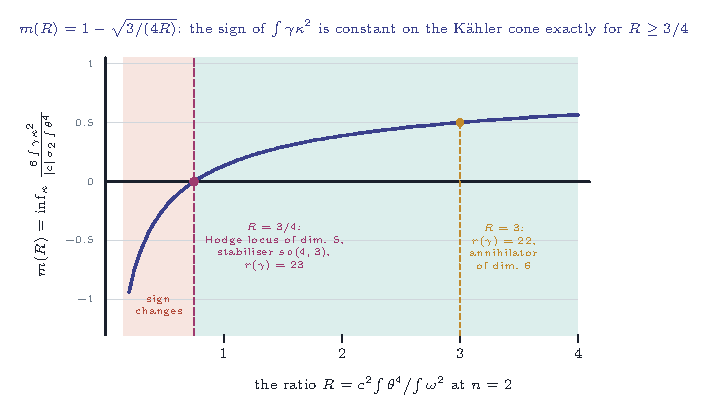
\includegraphics[width=0.86\textwidth]{fig_kahlersign}
\caption{The exceptional ratio of \Cref{rem:p2primeexceptional}. By the
identity displayed there, which is linear in $\gamma$, the infimum over the
K\"ahler cone of $6\int\gamma\kappa^{2}\big/\bigl(|c|\,\sigma_{2}(h)\int
\theta^{4}\bigr)$ is $m(R)=1-\sqrt{3/(4R)}$, approached at the boundary of the
cone by a positive hermitian form of rank two whose Pl\"ucker coordinates
satisfy $|\xi_{01}\xi_{23}|=\frac14$. It is negative exactly for $R<3/4$, and
$R=3/4$ is also where the Hodge locus of $\gamma$ jumps from dimension $4$ to
$5$ and its stabiliser becomes $\mathfrak{so}(4,3)$.}
\label{fig:kahlersign}
\end{figure}

\begin{remark}[The obstructions for a polarised character]
\label{rem:p2primesurvive}
The obstruction theorems proved from \cite[Section~9]{paperI} on for a Chern
character on the Weil line divide as follows for a polarised character. The
following hold unchanged, with
$r(\gamma)$ in place of $2n(2n-1)$ where a number occurs:
\cite[Theorem~9.20]{paperI} and \Cref{cor:noline}, whose only hypothesis is that
$\ch(E)$ stay of Hodge type to first order along $\cD_{n,n}$;
\Cref{thm:positivity} and \Cref{cor:nofiltered}, since a polarised character
is a flat Hodge class in every degree; \Cref{lem:finiteproduct}; and the
first two parts of \Cref{thm:p2numerical}, which become
\Cref{thm:p2primenumber}(iv). The following hold only when
$c_{0}=\dots=c_{2n-2}=0$, so that $H^{0,2}$ still kills $\gamma$:
\cite[Theorem~9.7]{paperI}, \cite[Proposition~9.10]{paperI}, \cite[Corollary~9.18]{paperI},
\cite[Theorem~9.19]{paperI} and \Cref{thm:p2forces}(iii). The following hold only
when $\ker H$ contains a vector with $w\ne0$, which needs $\rho\le2$, the
vector giving a compensated class of $P\wedge Q$ with a component in
$T_{+}\otimes T_{-}$: \Cref{thm:p2forces}(iv), \Cref{cor:p2shape} and
\Cref{thm:p2support}. The following do not extend: \Cref{thm:p2false},
outside \Cref{thm:p2primenumber}(v); the positivity of $\chi(E,E)$ in
\cite[Proposition~9.11]{paperI} and with it \Cref{thm:p2endo}(i)--(iii), by
\Cref{prop:p2primeprofile}(ii); and \cite[Theorem~2.32]{paperIII}. So for a general shape,
$\rho=3$, what these results exclude is a line bundle summand off the
polarisation line and a Chern character effective in the exponential basis,
and nothing else; \Cref{prop:scalaratiyah} below extends the first to
summands with a scalar Atiyah class. An object with no such summand, whose
Chern character is not effective, and with $\dim\Ext^{2}(E,E)=7n^{2}-2n$, is
not excluded by anything proved here, and none is known; by
\Cref{lem:p2primesummands} below it may be taken indecomposable.
\end{remark}

\begin{proposition}[Summands with a scalar Atiyah class]\label{prop:scalaratiyah}
Let $A$ be of $(K,-1,n)$-Weil type with $n\ge2$, let $T=T_{[A]}\cD_{n,n}$, and
let $E$ be a perfect complex on $A$ with $v\lrcorner\ch(E)=0$ for every
$v\in T$. Suppose $E$ has a direct summand $F[p]$ with
$\mathrm{At}(F)=\delta\cdot\id_{F}$, where $\delta$ is a real class of type
$(1,1)$ that is not a real multiple of $\theta$, and $\rk F\ne0$. Then there is
$v\in T$ with $\operatorname{ev}_{E}(v)\ne0$ and
$\sigma_{E}(\operatorname{ev}_{E}(v))=0$. In particular no finite direct sum
of shifted bundles $\pi_{*}L$, $\pi$ an isogeny, among them the simple
semi-homogeneous bundles, has a polarised character $\gamma$ with $N\ne0$ and
injective semiregularity map.
\end{proposition}

\begin{proof}
As in \cite[Theorem~9.20]{paperI}, $\operatorname{ev}_{E}(v)=v\lrcorner\mathrm{At}(E)$
on $H^{1}(T_{A})$ and the Atiyah class of a direct sum is block diagonal, so
the component of $\operatorname{ev}_{E}(v)$ in $\Ext^{2}(F,F)$ is
$(v\lrcorner\delta)\cdot\id_{F}$; the map $z\mapsto z\cdot\id_{F}$ on
$H^{0,2}$ is injective because $\mathrm{tr}(z\cdot\id_{F})=\rk(F)\,z$, and
some $v\in T$ has $v\lrcorner\delta\ne0$ by \cite[Proposition~9.15(i)]{paperI}. On the
other hand $\sigma_{E}(\operatorname{ev}_{E}(v))=v\lrcorner\ch(E)=0$. For the
last sentence, the proof of \Cref{lem:blocks}(i) gives
$\mathrm{At}(\pi_{*}L)=\delta\cdot\id$ with $\pi^{*}\delta=c_{1}(L)$ for any
line bundle $L$, and $\ch(\pi_{*}L)=\rk(\pi_{*}L)\,e^{\delta}$; if every
$\delta$ were a multiple of $\theta$ the Chern character of the sum would lie
in $\QQ[\theta]$, which does not contain $\omega$ because $\omega\theta=0$ and
$\theta^{n+1}\ne0$.
\end{proof}

\Cref{thm:semiregclosure} asks that $\sigma_{E}$ be injective, but its proof
uses only that the relative deformations of $E$ dominate the family, and
Pridham's form of \Cref{thm:BF}, in which $\sigma_{E}$ annihilates every
obstruction, gives this under a weaker hypothesis. That hypothesis allows an
object that is obstructed to first order, which is exactly the way in which
\cite[Theorem~9.20]{paperI}, \Cref{cor:noline} and \Cref{prop:scalaratiyah} exclude
an object.

\begin{proposition}[A flatness form of the criterion]\label{prop:p2flat}
Let $n\ge2$, $s_{0}\in\cD_{n,n}$, and let $E$ be a bounded complex of vector
bundles on $A_{s_{0}}$ with $\ch(E)=N\omega_{1}+\sum_{k}c_{k}\theta^{k}$ and
$N\ne0$. Let $K_{E}$ be the base of a miniversal deformation of $E$ on the
fixed variety $A_{s_{0}}$, put $e=\dim\Ext^{1}(E,E)$ and
$k=\dim\ker\sigma_{E}$. By \Cref{thm:BF} in Pridham's form, $\sigma_{E}$
annihilates every obstruction, both on $A_{s_{0}}$ and along the Artinian
deformations of $A_{s_{0}}$ in $\cD_{n,n}$.
\begin{enumerate}[label=\textup{(\roman*)},leftmargin=2.6em,itemsep=2pt]
\item $\dim K_{E}\ge e-k$.
\item If $\dim K_{E}=e-k$, then $\Sigma=\cD_{n,n}$, and the Hodge conjecture
  holds in every degree for every member of the family with
  $\Hg(A)=\SU(V,H)$.
\item $\dim K_{E}=e-k$ as soon as the cone
  $\{\xi\in\Ext^{1}(E,E):\xi\circ\xi=0\}$ has codimension $k$.
\end{enumerate}
For $k=0$ this is \Cref{thm:semiregclosure}.
\end{proposition}

\begin{proof}
Let $R$ be the completed local ring of $\cD_{n,n}$ at $s_{0}$, regular of
dimension $n^{2}$. By hypothesis $\ker\sigma_{E}$ is a complete obstruction
space for the deformations of the pair $(A_{s},E)$ over Artinian $R$-algebras,
whose relative tangent space is $\Ext^{1}(E,E)$; so this functor has a hull
$P/J$ with $P=R[[x_{1},\dots,x_{e}]]$ and $J$ generated by at most $k$
elements \cite{FM98}, and its fibre over the closed point of $R$ is a hull of
the absolute functor, of dimension $\dim K_{E}$. Krull's height theorem gives
$\dim P/J\ge n^{2}+e-k$, and the same count on the fibre gives (i). If
$\dim K_{E}=e-k$, the dimension inequality for a local homomorphism
\cite[Theorem~15.1]{Mat86} gives $\dim P/J\le n^{2}+e-k$, so equality holds, $J$
has height $k$ and is generated by a regular sequence, $P/J$ is
Cohen--Macaulay, and it is flat over $R$ by miracle flatness
\cite[Theorem~23.1]{Mat86}: a local homomorphism from a regular local ring to
a Cohen--Macaulay local ring is flat exactly when the dimension of the target
is the dimension of the source plus that of the fibre, and here both sides
equal $n^{2}+e-k$. The analytic Kuranishi germ of pairs, as in the
proof of \Cref{thm:p2false}, has $P/J$ as its completion, so it is flat over
the germ of $\cD_{n,n}$ at $s_{0}$ and therefore open onto a neighbourhood
$U$ of $s_{0}$. Every $A_{s}$ with $s\in U$ then carries a bounded complex of
vector bundles, algebraic by GAGA, whose Chern character is the parallel
transport of $\ch(E)$, so $N\omega_{1,s}$ differs from an algebraic class by a
polynomial in $\theta$ and is algebraic; \cite[Corollary~16.5]{paperI} gives (ii).
For (iii), the quadratic part of the Kuranishi map of $E$ is
$\xi\mapsto\xi\circ\xi$, so the tangent cone of $K_{E}$ lies in the cone of the
hypothesis, and $\dim K_{E}\le e-k$. Every step uses only deformations along
$\cD_{n,n}$, which are projective, whereas the proof of \Cref{thm:p2false}
needs non-projective ones.
\end{proof}

No object is known that meets (iii) with $k>0$. Among direct sums the
flatness form fails for a large class (\Cref{rem:flatsums} below); for
indecomposable objects nothing in this paper excludes it, and the proposition
says only that injectivity of $\sigma_{E}$ is more than propagation needs.

\subsection{Candidate objects for the polarised criterion}

The polarised criterion asks for one perfect complex. The results below say
what such a complex can be made of, for $K$ imaginary quadratic: a direct sum
meets the criterion only through one indecomposable summand
(\Cref{lem:p2primesummands}); no sum of objects whose Ext algebra is an
exterior algebra meets it (\Cref{cor:naturalsums}); the Orlov products of
secant objects meet its twisted form, with $\dim\Ext^{2}$ equal to the number
of \Cref{thm:p2primenumber}, at $n=2$ and $n=3$ (\Cref{thm:twistedcert}), and
cannot meet it at $n=4$ when the factors have no negative self-extensions
(\Cref{prop:orlovfour}); line bundles on smooth divisors, which give the
certificates, give no factor from $n=4$ on, nor do bundles restricted from
the abelian variety at $n=5$ (\Cref{prop:divisortemplate}); and at $n=4$ a combination of natural objects needs
at least eight of them, on one conic (\Cref{thm:minimalsupport}). None of
this gives a new case of the Hodge conjecture: the certificates are for
twisted objects, in families where Markman's theorem already holds.

\begin{lemma}[The summands of an object meeting the criterion]
\label{lem:p2primesummands}
Let $A$ be a member of a $(K,-1,n)$-Weil family, $K$ imaginary quadratic and
$n\ge2$, let $T=T_{[A]}\cD_{n,n}\subseteq H^{1}(T_{A})$, and let
$E=\bigoplus_{i}F_{i}[k_{i}]$ be a finite direct sum of perfect complexes with
$v\lrcorner\ch(E)=0$ for every $v\in T$, as holds for every polarised character
$N\omega_{1}+\sum_{k}c_{k}\theta^{k}$. Suppose that $\sigma_{E}$ is injective on
$\operatorname{ev}_{E}(T)$; this holds if $\sigma_{E}$ is injective, and under
the weakened criterion of \cite[Question 11.4]{Mar25b}.
\begin{enumerate}[label=\textup{(\roman*)},leftmargin=2.6em,itemsep=2pt]
\item For every $i$ and every $v\in T$, $\operatorname{ev}_{F_{i}}(v)=0$ and
  $v\lrcorner\ch(F_{i})=0$, and every $\ch(F_{i})$ lies in
  $\bigoplus_{k}\QQ\theta^{k}\oplus\HW(A)$.
\item If $\ch(E)=N\omega_{1}+\sum_{k}c_{k}\theta^{k}$ with $N\ne0$, some
  $F_{i}$ has $\ch(F_{i})=\omega'+\sum_{k}c'_{k}\theta^{k}$ with $\omega'$ a
  nonzero rational Weil class, and then
  $\dim\Ext^{2}(F_{i},F_{i})\ge r(\ch F_{i})\ge2n(2n-1)$. If $\sigma_{E}$ is
  injective, so is every $\sigma_{F_{i}}$, and that $F_{i}$ meets the polarised
  criterion on its own.
\end{enumerate}
So the polarised criterion is a statement about indecomposable objects.
\end{lemma}

\begin{proof}
For $v\in T$, $\sigma_{E}(\operatorname{ev}_{E}(v))=v\lrcorner\ch(E)=0$ by the
commutative square of \Cref{setup:criterion}, so $\operatorname{ev}_{E}(v)=0$.
The Atiyah class is natural, so $\operatorname{ev}_{E}(v)=v\lrcorner
\mathrm{At}(E)$ is block diagonal with the blocks $\pm\operatorname{ev}_{F_{i}}(v)$,
which therefore vanish, and $v\lrcorner\ch(F_{i})=\sigma_{F_{i}}
(\operatorname{ev}_{F_{i}}(v))=0$. By \Cref{prop:p2primelocus}(i) every
homogeneous component of $\ch(F_{i})$, a rational class of type $(k,k)$, stays
of Hodge type on the germ of $\cD_{n,n}$ at $A$, which in the chart of that
proposition is the linear space $T$; so it is a Hodge class at a member with
Hodge group $\SU(V,H)$, and \cite[Theorem~4.14]{paperI} puts it in $\QQ\theta^{k}$, or
in $\QQ\theta^{n}\oplus\HW$ for $k=n$. That is (i). For (ii), the Weil parts
of the $\pm\ch(F_{i})$ add up to $N\omega_{1}\ne0$, so one of them is nonzero;
\Cref{thm:p2primenumber} gives $\dim\Ext^{2}(F_{i},F_{i})\ge r(\ch F_{i})$ with
no hypothesis on $\sigma$, and $r\ge(4+0)n^{2}-2n=2n(2n-1)$ for $n\ge3$, while
at $n=2$ the seven values of \Cref{fig:hankel} are at least $12$. Injectivity
passes to the summands by \cite[Lemma~3.38]{paperIII}. By the Krull--Schmidt property
of $D^{b}(A)$ the $F_{i}$ may be taken indecomposable.
\end{proof}

The Weil part $\omega'$ of the summand need not be a multiple of $\omega_{1}$;
propagating any nonzero rational Weil class propagates the whole Weil plane,
through the algebraic action of $K$. The lemma is the Weil-family analogue of
\cite[Corollary~3.41(ii)]{paperIII}.

\begin{corollary}[Sums of objects with exterior Ext algebras]
\label{cor:naturalsums}
In \Cref{lem:p2primesummands}, let every $F_{i}$ have
$\dim\Ext^{2}(F_{i},F_{i})<2n(2n-1)$. This holds when
$\Ext^{*}(F_{i},F_{i})\cong\bigwedge^{*}\CC^{2n}$, and so for line bundles, for
the sheaves $\cO_{B}\otimes L$ with $B\subseteq A$ an abelian subvariety, for
simple semi-homogeneous bundles, for skyscraper sheaves, and for the images of
all of these under autoequivalences of $D^{b}(A)$. Then no such sum with
$\ch(E)=N\omega_{1}+\sum_{k}c_{k}\theta^{k}$ and $N\ne0$ has $\sigma_{E}$
injective on $\operatorname{ev}_{E}(T)$: it fails the polarised criterion and
the weakened criterion, some $v\in T$ obstructs it to first order, and
$\dim\Ext^{2}(E,E)>r(\ch E)$.
\end{corollary}

\begin{proof}
The first assertion is \Cref{lem:p2primesummands}(ii), since
$\binom{2n}{2}=n(2n-1)<2n(2n-1)$, and $\dim\Ext^{2}(E,E)\ge r(\ch E)$ with
equality only if $\sigma_{E}$ is injective (\Cref{thm:p2primenumber}). For
$\cO_{B}$ choose a complementary abelian subvariety $B'$; the isogeny
$\mu\colon B\times B'\to A$ is \'etale with group $G=B\cap B'$, and
$\mu^{*}\cO_{B}=\bigoplus_{g\in G}\cO_{B\times\{g\}}$ with $G$ permuting the
summands simply transitively, so $\Ext_{A}(\cO_{B},\cO_{B})
=\Ext_{B\times B'}(\cO_{B\times0},\cO_{B\times0})=\bigwedge^{*}(\CC^{\dim B}
\oplus\CC^{\dim B'})$. For a simple semi-homogeneous bundle $V$,
$V\otimes V^{\vee}$ is a sum of line bundles in $\Pic^{0}$ of which $\cO$ occurs
once \cite{Muk78}, so $\Ext^{*}(V,V)=H^{*}(\cO_{A})$. Equivalences preserve
Ext algebras.
\end{proof}

By \Cref{lem:p2primesummands} the objects that \Cref{rem:p2primesurvive}
allows may be taken indecomposable. The corollary recovers, for
polarised characters, the part of \cite[Theorem~2.32]{paperIII} that concerns objects with
exterior Ext algebras, and it extends \Cref{prop:scalaratiyah}, whose summand
has a scalar Atiyah class, to the subtori, the points and the Fourier--Mukai
images. In the language of pure spinors, a summand whose
character is a rational multiple of the pure spinor of a rational maximal
isotropic subspace is excluded unless that character lies in $\QQ[\theta]$,
because the rational maximal isotropic subspaces whose pure spinors are flat
over $\cD_{n,n}$ are those with pure spinor $1$, the class of a point or
$e^{c\theta}$.

The secant objects of \cite[Section~14]{paperI} have their own Hochschild
profile, which \Cref{thm:factor}(i) and (ii) compute in degrees one and two.

\begin{proposition}[The Hochschild profile of a secant class]
\label{prop:secantprofile}
Let $X$ be a principally polarised abelian $n$-fold, $n\ge2$, with
polarisation $\theta$, let $d\ge1$, and let $v=a\,u_{\theta}+b\,v_{\theta}$
with $(a,b)\in\QQ^{2}\setminus\{0\}$, in the notation of \cite[(30)]{paperI}. The
rank of contraction $HT^{k}(X)\to H^{*}(X,\CC)$, $\xi\mapsto\xi\lrcorner v$, is
$1$ for $k=0$ and $k=n$, $2\binom{n}{k}$ for $1\le k\le n-1$, and $0$ for
$k>n$. A perfect complex $F$ on $X$ with $\ch(F)=v$ has
$\dim\Ext^{k}(F,F)\ge2\binom{n}{k}$ for $k=1,2$, and
\[
  \chi(F,F)=\begin{cases}
    (-1)^{n/2}\,2^{n-1}d^{\,n/2-1}(a^{2}d+b^{2}) & n\text{ even},\\
    0 & n\text{ odd}.
  \end{cases}
\]
\end{proposition}

\begin{proof}
Put $s=\sqrt{-d}$ and $w=\frac12(a-bs/d)$. By \cite[Theorem~14.5(i)]{paperI},
$v=w\,e^{s\theta}+\bbar w\,e^{-s\theta}$, and $w\ne0$. By
\Cref{lem:bfield}(i), $\xi\lrcorner e^{\pm s\theta}=y_{\pm}e^{\pm s\theta}$,
where $y_{\pm}\in H^{0,k}(X)$ is the component of $e^{\pm s\theta}\xi$ in
$\bigwedge^{k}H^{0,1}$. The map $\xi\mapsto(y_{+},y_{-})$ is onto
$H^{0,k}\oplus H^{0,k}$ for $k\ge1$: $\xi=z\in\bigwedge^{k}H^{0,1}$ gives
$(z,z)$, and $\xi=z'\otimes\partial$ with $z'\in\bigwedge^{k-1}H^{0,1}$ gives
$\pm s\,z'\wedge(\partial\lrcorner\theta)$, where $\partial\lrcorner\theta$ runs
over $H^{0,1}$. If $w\,y_{+}e^{s\theta}+\bbar w\,y_{-}e^{-s\theta}=0$, the
components of degrees $k$ and $k+2$ give $wy_{+}+\bbar wy_{-}=0$ and
$(wy_{+}-\bbar wy_{-})\wedge\theta=0$, and for $k<n$ wedge product with
$\theta=\sum_{a}p_{a}\wedge q_{a}$ is injective on $\bigwedge^{k}H^{0,1}$, so
$y_{\pm}=0$. So the rank is $2\binom{n}{k}$ for $1\le k<n$. For $k=n$,
$y\wedge\theta=0$ for $y\in H^{0,n}$ and the image is the line spanned by
$wy_{+}+\bbar wy_{-}$; for $k>n$, $H^{0,k}=0$; and for $k=0$ the rank is one.
The bounds on $\Ext^{1}$ and $\Ext^{2}$ follow, as in \Cref{thm:factor}(i)
and (ii), from the compatibility of the characteristic morphism with
contraction into the Chern character. Finally the Todd class
is trivial, so $\chi(F,F)=\int_{X}\ch(F)^{\vee}\ch(F)$ with
$\ch(F)^{\vee}=w\,e^{-s\theta}+\bbar w\,e^{s\theta}$, and
$\int_{X}(e^{2s\theta}+e^{-2s\theta})=(2s)^{n}(1+(-1)^{n})$ because
$\int_{X}\theta^{n}=n!$; with $|w|^{2}=(a^{2}d+b^{2})/(4d)$ this is the
formula.
\end{proof}

At $n=4$ and $(a,b)=(1,3)$, the class of \Cref{prop:markman8}, this gives
$\chi(\cF,\cF)=8d(d+9)$, the rank recorded there.

\begin{theorem}[Twisted certificates at $n=2$ and $n=3$]
\label{thm:twistedcert}
Let $d\ge1$, $K=\QQ(\sqrt{-d})$, let $\Phi$ be Orlov's equivalence of
\Cref{prop:markman8}(v), and for a perfect complex $F$ on a principally
polarised $X$ put $E=\Phi(F\boxtimes F^{\vee})$ on $A=X\times\widehat{X}$,
with the $K$-action of \cite[(29)]{paperI}, the Poincar\'e class $\ell$ and the
polarisation $\eta=d\beta+\widehat\beta$ of the split member
(\cite[Notation~15.1]{paperI}).
\begin{enumerate}[label=\textup{(\roman*)},leftmargin=2.6em,itemsep=2pt]
\item Let $X$ be the Jacobian of a curve $C$ of genus two, $C\subset X$ by an
  Abel--Jacobi map, and $F=\cO_{C}(p)$ for a point $p\in C$. Then
  $\ch(F)=v_{\theta}$, $\dim\Ext^{k}(F,F)=1,4,1$, and
  $\dim\Ext^{k}(E,E)=1,8,18,8,1$ for $k=0,\dots,4$, which are the ranks of
  contraction from $HT^{k}(A)$ into $\ch(E)$. So
  $\dim\Ext^{2}(E,E)=18=r(\ch E)$ and $\sigma_{E}$ is injective.
\item Let $X$ be the Jacobian of a non-hyperelliptic curve $C$ of genus three,
  $i\colon C^{(2)}\to X$ the embedding of the theta divisor, $x$ the class of
  $\{p+q:q\in C\}$ and $\theta$ the restriction of the polarisation, and let
  $d=k(k+1)$ with $k\ge1$ and $F=i_{*}\cO_{C^{(2)}}((2k+1)x-k\theta)$. Then
  $\ch(F)=v_{\theta}$, $\dim\Ext^{k}(F,F)=1,6,6,1$, and
  $\dim\Ext^{k}(E,E)=1,12,48,74,48,12,1$. So $\dim\Ext^{2}(E,E)=48=r(\ch E)$
  and $\sigma_{E}$ is injective.
\item In both cases $\ch(E)$ is not killed by $T=T_{[A]}\cD_{n,n}$, and no
  line bundle twist of $E$ has a character killed by $T$; the twisted
  character $\kappa=\ch(E)e^{\ell/2}$ is killed by $T$, has the form
  $N'\omega'+\sum_{k}c_{k}\eta^{k}$ with $\omega'$ a nonzero rational Weil
  class, and has the same contraction ranks as $\ch(E)$. A class
  $B\in\NS(A)_{\QQ}$ with $\ch(E)e^{B}$ killed by $T$ is congruent to $\ell/2$
  modulo $\QQ\eta$. At $n=2$,
  $\kappa$ has $c_{1}=c_{3}=0$ and lies at the exceptional ratio of
  \Cref{rem:p2primeexceptional}, and its annihilator in $H^{1}(T_{A})$ has
  dimension $5$; at $n=3$ that annihilator has dimension $9=n^{2}$.
\end{enumerate}
\end{theorem}

\begin{proof}
(i) By Grothendieck--Riemann--Roch $\ch(i_{*}\cO_{C}(p))=[C]+(1+1-2)[\mathrm{pt}]
=\theta=v_{\theta}$, since $v_{\theta}=\theta$ when $n=2$. For the curve,
$\Ext^{1}(\cO_{C},\cO_{C})=H^{1}(\cO_{C})\oplus H^{0}(N_{C})$ with
$N_{C}=K_{C}$ by adjunction, of dimension $2+2$, and $\Ext^{0}=\Ext^{2}=\CC$ by
Serre duality; twisting by $\cO_{C}(p)$ changes nothing. The Ext algebra of
$F^{\vee}$ is that of $F$, $\Phi$ is an equivalence, and by the K\"unneth
formula $\Ext^{*}(E,E)=\Ext^{*}(F,F)\otimes\Ext^{*}(F^{\vee},F^{\vee})$, which
gives $1,8,18,8,1$. By \Cref{prop:secantprofile} and the K\"unneth
decomposition $HT^{2}(X\times X)=HT^{2}\otimes1\oplus HT^{1}\otimes HT^{1}\oplus
1\otimes HT^{2}$ the rank of contraction into $\ch(F)\boxtimes\ch(F^{\vee})$ is
$1+4\cdot4+1=18$, and it is transported by $\Phi$ as in the proof of
\Cref{thm:factor}(iv). The other degrees are the same count. Equality in
degree two forces $\sigma_{E}$ injective, as in \Cref{thm:p2primenumber}.
(ii) On $C^{(2)}$ one has $x^{2}=1$, $x\theta=3$, $\theta^{2}=6$ and
$K_{C^{(2)}}=\theta$, $i_{*}x=\frac12\Theta^{2}$ and $i_{*}\theta=\Theta^{2}$, so
Riemann--Roch gives $\ch_{2}(F)=0$ and $\ch_{3}(F)=-k(k+1)[\mathrm{pt}]$, that
is $\ch(F)=\Theta-d[\mathrm{pt}]=v_{\theta}$. The local-to-global spectral
sequence, with $h^{p}(\cO_{C^{(2)}})=1,3,3$ and $h^{p}(K_{C^{(2)}})=3,3,1$,
gives $\dim\Ext^{1},\dim\Ext^{2}\le6$, and \Cref{prop:secantprofile} gives
$\ge6$; $\Ext^{0}=\CC$ and Serre duality gives $\Ext^{3}=\CC$. The rest is as
in (i), with $r(\ch E)=6n^{2}-2n=48$ by \Cref{thm:factor}(iv).

(iii) By \Cref{prop:flatall} below, whose proof does not use this theorem,
$\kappa$ lies in $\QQ[\eta]\oplus\HW(A)$ and is killed by $T$; both summands
are defined over $\QQ$, so its Weil part $N'\omega'$ is rational, and
$r(\kappa)=r(\ch E)$ is \Cref{lem:bfield}(i). The proof of
\Cref{prop:flatall} also gives $\kappa$ explicitly. At $n=2$,
$\ch(F)=\theta=\frac{1}{2s}(e^{s\theta}-e^{-s\theta})$ and
$\ch(F^{\vee})=-\theta$, so, with $t=s/2d$,
\[
  \kappa=-\bigl(e^{t\eta}+e^{-t\eta}\bigr)-\tfrac{1}{4d}\bigl(\gamma^{2}-d\ell^{2}\bigr)
  =-2+\tfrac{1}{4d}\eta^{2}-\tfrac{1}{192d^{2}}\eta^{4}
   -\tfrac{1}{4d}\bigl(\gamma^{2}-d\ell^{2}\bigr).
\]
Hence $c_{1}=c_{3}=0$ and $c_{2}=1/4d$. Write $\gamma-s\ell=a_{1}+a_{2}$ and
$\gamma+s\ell=b_{1}+b_{2}$ for the decompositions over the two factors of
$X=E_{1}\times E_{2}$, as in the proof of \Cref{prop:flatall}. Then
$a_{i}^{2}=b_{i}^{2}=0$, so the Weil part is
$\omega=-\frac{1}{4d}(a_{1}a_{2}+b_{1}b_{2})$, and
$a_{i}b_{i}=\gamma_{i}^{2}+d\ell_{i}^{2}=-4d\,\beta_{i}\widehat\beta_{i}$; so
$\int\omega^{2}=\frac{2}{16d^{2}}\int a_{1}b_{1}a_{2}b_{2}=2$, while
$\int\eta^{4}=6\int\eta_{1}^{2}\eta_{2}^{2}=24d^{2}$. Thus
$c_{2}^{2}\int\eta^{4}=\frac32=\frac34\int\omega^{2}$, the exceptional ratio of
\Cref{prop:p2primelocus}(iv), where the annihilator has dimension $5$. At
$n=3$, $\ch(F)=v_{\theta}=\frac{1}{2s}(e^{s\theta}-e^{-s\theta})$ and
$\ch(F^{\vee})=-v_{\theta}$, and the same computation gives the
$\eta$-part $-2s(e^{t\eta}-e^{-t\eta})=2\eta+\cdots$; so $c_{1}=2\ne0$ and the
annihilator is $T_{[A]}\cD_{3,3}$, of dimension $9$, by
\Cref{prop:p2primelocus}(iii).

For $B$, put $B'=B-\frac12\ell$, so that $\ch(E)e^{B}=\kappa e^{B'}$.
Contraction with $v\in T$ is a derivation and kills $\kappa$, so
$v\lrcorner(\kappa e^{B'})=\kappa\,(v\lrcorner B')\,e^{B'}$. Multiplication by
$\kappa$ is injective on $H^{2}(A,\CC)$: at $n=2$ the degree zero part of
$\kappa$ is $-2$, and at $n=3$ its lowest part is $2\eta$, and multiplication
by $\eta$ is injective from $H^{2}$ to $H^{4}$ on the sixfold $A$. So $T$ kills
$\kappa e^{B'}$ exactly when $v\lrcorner B'=0$ for all $v\in T$. By
\Cref{prop:p2primelocus}(i) the real class $B'$ of type $(1,1)$ then stays of
type $(1,1)$ on the germ of $\cD_{n,n}$ at $A$, hence on all of $\cD_{n,n}$, and
at a very general member $\NS\otimes\QQ=\QQ\eta$ (\cite[Lemma~7.5]{paperI}); so
$B'\in\QQ\eta$. The classes $x_{j}\xi_{j}$ appear in $\frac12\ell+c\eta$ with
coefficient $\frac12$ for every $c$, so no integral class is congruent to
$\frac12\ell$ modulo $\QQ\eta$, on any $X$: no line bundle twist of $E$, and in
particular not $E$ itself, has a character killed by $T$.
\end{proof}

In both cases the numerical form of the criterion holds with equality, so the
injectivity of $\sigma_{E}$ comes out of a dimension count and does not need
\cite[Question 11.4]{Mar25b}. The certificates concern the twisted object
only: the character $\kappa$ stays of Hodge type along $\cD_{n,n}$, while
$\ch(E)$ does
so only on a locus of dimension $3$ at $n=2$ and $6$ at $n=3$, so propagation
needs the extension of \Cref{thm:BF} to twisted objects, which Perry proves
\cite{Per26}, and an argument extracting untwisted cycles, as in
\cite[Section 2]{Mar25b}. The families concerned, of trivial discriminant with
$n=2$ and $n=3$, are Markman's.

\begin{proposition}[No Orlov product at $n=4$]\label{prop:orlovfour}
Let $X$ be a principally polarised abelian fourfold, $d\ge1$, and
$F_{1},F_{2}$ perfect complexes on $X$ with characters in the secant plane
$P_{\theta}\setminus\{0\}$ and $\Ext^{<0}(F_{i},F_{i})=0$, for instance
sheaves. Then $E=\Phi(F_{1}\boxtimes F_{2}^{\vee})$ has
$\dim\Ext^{2}(E,E)>88=r(\ch E)$.
\end{proposition}

\begin{proof}
By the K\"unneth formula $\dim\Ext^{2}(E,E)=e_{0}e_{2}'+e_{1}e_{1}'+e_{2}e_{0}'$
with $e_{k}=\dim\Ext^{k}(F_{1},F_{1})$ and $e_{k}'$ likewise for $F_{2}$, and by
\Cref{prop:secantprofile} $e_{0}\ge1$, $e_{1}\ge8$, $e_{2}\ge12$; so the sum is
at least $12+64+12=88$, which is $r(\ch E)$ by \Cref{thm:factor}(iv). Equality
would force $e_{0},e_{1},e_{2}=1,8,12$. Since $e_{k}=0$ for $k<0$ and Serre
duality gives $e_{k}=e_{4-k}$, this would give
$\chi(F_{1},F_{1})=1-8+12-8+1=-2$, while \Cref{prop:secantprofile} gives
$\chi(F_{1},F_{1})=8d(a^{2}d+b^{2})>0$.
\end{proof}

Without $\Ext^{<0}=0$ the count changes, because negative Ext groups of the
$F_{i}$ contribute products $e_{-j}e_{2+j}'$ to $\Ext^{2}(E,E)$ and change the
Euler characteristic. The next two results treat the template in every
dimension: the twisted character is always flat, and the count says exactly
which secant objects would give equality.

\begin{proposition}[Flatness in every dimension]\label{prop:flatall}
Let $(X,\theta)$ be a principally polarised abelian $n$-fold, $n\ge1$, let
$d\ge1$ and $s=\sqrt{-d}$, and put $\Psi(Z)=\ch\bigl(\Phi(Z)\bigr)e^{\ell/2}$
for classes $Z$ on $X\times X$, extended linearly, with $\gamma=d\beta-\widehat\beta$
as in \cite[Theorem~15.2]{paperI} and $\eta=d\beta+\widehat\beta$. For $\sigma=\pm1$, $\Psi(e^{\sigma s\theta}\boxtimes
e^{\sigma s\theta})$ is a nonzero multiple of $e^{\sigma(s/2d)\eta}$, and
$\Psi(e^{\sigma s\theta}\boxtimes e^{-\sigma s\theta})$ is a nonzero multiple of the
Weil class $(\gamma-\sigma s\ell)^{n}$. Consequently, for perfect complexes
$F_{1},F_{2}$ with $\ch(F_{i})\in P_{\theta}$, the class
$\kappa=\ch\bigl(\Phi(F_{1}\boxtimes F_{2}^{\vee})\bigr)e^{\ell/2}$ lies in
$\QQ[\eta]\oplus\HW(A)$, is killed by $T=T_{[A]}\cD_{n,n}$, and has Hankel rank
$\rho\le2$; for $F_{1}=F_{2}\ne0$ its Weil part is nonzero.
\end{proposition}

\begin{proof}
A symplectic basis of $H^{1}(X,\ZZ)$ for $\theta$ identifies $H^{*}(X,\QQ)$,
with $\theta$, with the tensor product of $n$ copies of the cohomology of an
elliptic curve with its class $\theta_{i}$, $\theta=\sum_{i}\theta_{i}$. The
action of $\Phi$ on cohomology is the correspondence $(1\times\Phi_{P})\circ
\mu_{*}$ with $\mu(a,b)=(a-b,b)$, and $\mu$, the Poincar\'e class
$\ell=\sum_{i}\ell_{i}$, the classes $\eta$ and $\gamma$, and the exponentials
$e^{\pm s\theta}=\bigotimes_{i}e^{\pm s\theta_{i}}$ all decompose as tensor
products over $i$ of classes of even degree, so no signs arise. Each identity
is therefore the tensor product of $n$ copies of the identity for $n=1$, up to
a nonzero scalar, where for the Weil class one uses
$(\gamma-\sigma s\ell)^{n}=n!\prod_{i}(\gamma_{i}-\sigma s\ell_{i})$, valid because
the factors commute and $(\gamma_{i}-\sigma s\ell_{i})^{2}=0$: by
\cite[Theorem~15.2(i)]{paperI} at $n=1$ the class $\gamma_{i}-\sigma s\ell_{i}$
spans the top exterior power of a two-dimensional eigenspace.

It remains to treat $n=1$. Let $y_{1},y_{2}$ be a symplectic basis of
$H^{1}(X)$, $z_{1},z_{2}$ its copy on the second factor of $X\times X$ and
$\xi_{1},\xi_{2}$ the dual basis of $H^{1}(\widehat X)$, so that
$\theta=\beta=y_{1}y_{2}$, $\widehat\beta=\xi_{1}\xi_{2}$,
$\ell=y_{1}\xi_{1}+y_{2}\xi_{2}$ and $\ell^{2}=-2\beta\widehat\beta$. On
cohomology $\Phi$ sends $w$ to $\int_{z}\mu^{*}w\cdot e^{z_{1}\xi_{1}+z_{2}\xi_{2}}$,
the integral being over the second factor; with the opposite sign of the
Poincar\'e class, $\ell$ is replaced by $-\ell$ in this proposition and in
\Cref{thm:twistedcert}. For $a,b\in\{\pm1\}$,
\begin{gather*}
  \mu^{*}\bigl(e^{as\theta}\boxtimes e^{bs\theta}\bigr)
  =\bigl(1+as(y_{1}+z_{1})(y_{2}+z_{2})\bigr)\bigl(1+bs\,z_{1}z_{2}\bigr),\\
  e^{z_{1}\xi_{1}+z_{2}\xi_{2}}=1+z_{1}\xi_{1}+z_{2}\xi_{2}-z_{1}z_{2}\xi_{1}\xi_{2},
\end{gather*}
and collecting the coefficient of $z_{1}z_{2}$ in the product gives
\[
  \ch\Phi\bigl(e^{as\theta}\boxtimes e^{bs\theta}\bigr)
  =(a+b)s-ab\,d\,\beta-\widehat\beta-as\,\ell-as\,\beta\widehat\beta .
\]
Multiplying by $e^{\ell/2}=1+\frac12\ell-\frac14\beta\widehat\beta$, and using
$\beta\ell=\widehat\beta\ell=0$, gives
$\Psi=2as-d\beta-\widehat\beta-\frac{as}{2}\beta\widehat\beta=2as\,e^{(as/2d)\eta}$
when $a=b$, and $\Psi=d\beta-\widehat\beta-as\ell=\gamma-as\ell$ when $a=-b$.
So for general $n$ the multiples are $(2\sigma s)^{n}$ and $1/n!$.

For the consequence, write
$\ch(F_{1})=w_{1}e^{s\theta}+\bbar w_{1}e^{-s\theta}$ and
$\ch(F_{2}^{\vee})=w_{2}e^{-s\theta}+\bbar w_{2}e^{s\theta}$ as in the proof of
\Cref{prop:secantprofile}; the terms $e^{\pm s\theta}\boxtimes e^{\pm s\theta}$
give multiples of $e^{\pm(s/2d)\eta}$ and the mixed terms give the Weil part
$w_{1}w_{2}c_{+}\alpha_{+}+\bbar w_{1}\bbar w_{2}c_{-}\alpha_{-}$, with
$c_{\pm}\ne0$. The classes of $\QQ[\eta]\oplus\HW(A)$ are Hodge classes on
every member of the family, so $T$ kills $\kappa$, and the $\eta$-part lies in
the span of the two exponentials $e^{\pm(s/2d)\eta}$, which gives $\rho\le2$.
\end{proof}

\begin{proposition}[The equality criterion for the Orlov template]
\label{prop:orlovequality}
Let $(X,t)$ be a polarised abelian $n$-fold, $n\ge2$, $d\ge1$, and $F_{1}$,
$F_{2}$ perfect complexes with characters in $P_{t}\setminus\{0\}$; put
$e_{k}=\dim\Ext^{k}(F_{1},F_{1})$ and $e_{k}'=\dim\Ext^{k}(F_{2},F_{2})$ for all
$k\in\ZZ$, and $E=\Phi(F_{1}\boxtimes F_{2}^{\vee})$.
\begin{enumerate}[label=\textup{(\roman*)},leftmargin=2.6em,itemsep=2pt]
\item $\dim\Ext^{2}(E,E)=\sum_{k\in\ZZ}e_{k}e_{2-k}'\ge R_{n}$, where
  $R_{n}=6n^{2}-2n$ for $n\ge3$ and $R_{2}=18$, and $R_{n}=r(\ch E)=r(\kappa)$.
\item Equality holds if and only if $(e_{0},e_{1},e_{2})=(e_{0}',e_{1}',e_{2}')
  =(1,2n,r_{2})$, with $r_{2}=n(n-1)$ for $n\ge3$ and $r_{2}=1$ for $n=2$, and
  $e_{-j}e_{2+j}'=e_{2+j}e_{-j}'=0$ for every $j\ge1$.
\item For $F_{1}=F_{2}=F$ and $n\ge3$ the last condition says that the set
  $S=\{j\ge1:\Ext^{-j}(F,F)\ne0\}$ lies in $[n-1,\infty)$ and that $j\in S$
  implies $j-(n-2)\notin S$; for $n=2$ it says $\Ext^{<0}(F,F)=0$.
\item Equality implies that $\sigma_{E}$ is injective.
\end{enumerate}
\end{proposition}

\begin{proof}
(i) $\Phi$ is an equivalence and the K\"unneth formula holds in all degrees,
negative ones included, and dualising is an anti-equivalence, so
$\Ext^{*}(E,E)=\Ext^{*}(F_{1},F_{1})\otimes\Ext^{*}(F_{2},F_{2})$. By
\Cref{prop:secantprofile}, $e_{0}\ge1$, $e_{1}\ge2n$ and $e_{2}\ge r_{2}$, so the
three terms with $k=0,1,2$ already give $R_{n}$; the equality $R_{n}=r(\ch E)$ is
the K\"unneth count of \Cref{thm:factor}(iv) and \Cref{thm:twistedcert}, and
$r(\kappa)=r(\ch E)$ by \Cref{lem:bfield}(i). (ii) Every term is nonnegative,
and $e_{0}e_{2}'\ge e_{2}'\ge r_{2}>0$ with equality only if $e_{0}=1$ and
$e_{2}'=r_{2}$, and likewise for the other two terms; every other product must
vanish. (iii) Serre duality gives $e_{k}=e_{n-k}$. For $1\le j\le n-2$, $e_{2+j}$ is
at least the rank of contraction from $HT^{2+j}(X)$ into $\ch(F)$, which is
positive by \Cref{prop:secantprofile}, because the characteristic morphism is
compatible with contraction into the Chern character in every degree
\cite{CRV12}; so $e_{-j}=0$. For $j\ge n-1$, $e_{2+j}=e_{-(j-(n-2))}$.
(iv) The composite $\sigma_{E}\circ\operatorname{ev}_{E}$
is contraction into $\ch(E)$, of rank $R_{n}\le\operatorname{rk}\sigma_{E}\le
\dim\Ext^{2}(E,E)$, so equality forces $\sigma_{E}$ to be injective.
\end{proof}

For $n=2$ and $n=3$ the certificates of \Cref{thm:twistedcert} attain the
equality; for $n=4$ it is excluded by \Cref{prop:orlovfour} when
$\Ext^{<0}=0$, with negative Ext groups in degrees at most $-(n-1)$ the
Euler characteristic leaves room in every dimension, and from $n=5$ on it
leaves room without them (\Cref{prop:divisortemplate}(i)). If a secant object $F$
attaining the equality existed for one $d$ and unboundedly many $n$, then,
since $\kappa$ is flat in every dimension by
\Cref{prop:flatall}, a twisted form of \Cref{thm:semiregclosure} together with
\cite[Proposition~2.13]{paperIII} would make the Weil classes of every family of
$\QQ(\sqrt{-d})$ algebraic. That is the secant route of (C1) and (C2) in
\cite[Section~2.5]{paperIII}, with the question of \cite{Mar25b} replaced by a
dimension count, and it lies off every minimal route (\cite[Theorem~2.70(iv)]{paperIII}).

Both certificates are sheaves on theta divisors, a curve of genus two and the
surface $C^{(2)}$. The next result explains why this construction stops at
$n=3$ and what a continuation would need.

\begin{proposition}[Sheaves on divisors in the Orlov template]
\label{prop:divisortemplate}
Let $(X,\theta)$ be a principally polarised abelian $n$-fold and $d\ge1$; put
$S(x)=\sum_{j\ge0}(-d)^{j}x^{2j}/(2j+1)!$, so that $v_{\theta}=\theta
S(\theta)$, and $T_{b}(x)=bx/(1-e^{-bx})$ for an integer $b\ge1$. Write
$\beta_{0}=\beta_{n}=1$, $\beta_{k}=2\binom{n}{k}$ for $0<k<n$ and
$\beta_{k}=0$ otherwise; these are the Betti numbers of the connected sum of
two real $n$-tori.
\begin{enumerate}[label=\textup{(\roman*)},leftmargin=2.6em,itemsep=2pt]
\item Let $n\ge5$ and let $F$ be a perfect complex with
  $\ch(F)\in P_{\theta}\setminus\{0\}$. There are integers $e_{k}$, zero for
  $k\notin[0,n]$, with $e_{k}=e_{n-k}$, $(e_{0},e_{1},e_{2})=(1,2n,n(n-1))$,
  $e_{k}\ge\beta_{k}$ for all $k$, and $\sum_{k}(-1)^{k}e_{k}=\chi(F,F)$. So
  Serre duality, the contraction bounds $e_{k}\ge\beta_{k}$
  (\Cref{prop:secantprofile} and \cite{CRV12}) and the Euler
  characteristic allow equality in \Cref{prop:orlovequality} with
  $\Ext^{<0}(F,F)=0$. For odd $n$ one may take $e_{k}=\beta_{k}$, and at $n=5$
  this is the only choice; for even $n$ the sequence $(\beta_{k})$ has Euler
  characteristic $-2\ne\chi(F,F)$, so some $e_{k}$ with $3\le k\le n-3$ must
  exceed $\beta_{k}$.
\item Let $n\ge3$, let $i\colon D\hookrightarrow X$ be a smooth effective
  divisor, and let $G$ be a vector bundle of rank $r\ge1$ on $D$ with
  $\ch(G)\in i^{*}H^{*}(X,\QQ)$. If $\ch(i_{*}G)\in P_{\theta}$, then
  $[D]=b\theta$ for an integer $b\ge1$ and
  $\ch(G)=r\,i^{*}\bigl(S(\theta)\,T_{b}(\theta)\bigr)$; in particular
  $c_{1}(G)=\frac{rb}{2}\,\theta|_{D}$,
  $\ch_{2}(G)=r\bigl(\frac{b^{2}}{12}-\frac{d}{6}\bigr)\theta^{2}|_{D}$ and
  $r\ge2$. If $n\ge4$, every line bundle on $D$ satisfies the hypothesis, so
  no line bundle $L$ on a smooth divisor has $\ch(i_{*}L)\in P_{\theta}$, and
  $rb$ is even. If $n\ge5$, $b=1$ and $r=2$, then
  $c_{2}(G)=\frac{d+1}{3}\,\theta^{2}|_{D}$, which is integral only for
  $d\equiv2\pmod3$.
\item Let $n\ge2$, let $i\colon D\hookrightarrow X$ be a smooth divisor with
  $[D]=b\theta$, $V$ a vector bundle on $X$, $G=V|_{D}$ and $F=i_{*}G$. Then
  \[
    \dim\Ext^{k}(F,F)=h^{k}(\End G)+h^{k-1}\bigl(\End G\otimes\cO_{D}(D)\bigr)
  \]
  for every $k$. For $b=1$ this is
  $\beta_{k}+h^{k}(\End_{0}G)+h^{k-1}(\End_{0}G\otimes\cO_{D}(D))$, so for a line
  bundle $V$ the sheaf $F$ has exactly the profile required in
  \Cref{prop:orlovequality}(ii). For $b\ge2$, $\dim\Ext^{1}(F,F)\ge
  b^{n}+n-1>2n$.
\item At $n=5$, for no smooth divisor $D$ and no vector bundle $V$ on $X$ is
  $i_{*}(V|_{D})$ a factor of an Orlov product attaining the equality of
  \Cref{prop:orlovequality}.
\end{enumerate}
\end{proposition}

\begin{proof}
(i) The rank $a$ of $F$ is an integer, and $c_{1}(F)=b\theta$ with $\theta$
primitive, so $b\in\ZZ$; for even $n$ the number
$c=2^{n-1}d^{n/2-1}(a^{2}d+b^{2})$ is therefore a positive integer divisible
by $2^{n-1}$, and $\chi(F,F)=(-1)^{n/2}c$ by \Cref{prop:secantprofile}, while
$\chi(F,F)=0$ for odd $n$. The conditions fix $e_{0},e_{1},e_{2}$ and, by
symmetry, $e_{n-2},e_{n-1},e_{n}$, with the values $\beta_{k}$; for $n=5$ these
are all the $e_{k}$. Since $\sum_{k=0}^{n}(-1)^{k}\binom{n}{k}=0$, the
sequence $(\beta_{k})$ has Euler characteristic $0$ for odd $n$ and $-2$ for
even $n$. For odd $n$ take $e_{k}=\beta_{k}$. For even $n\ge6$ take
$e_{k}=\beta_{k}$ for $k\ne n/2$ and
$e_{n/2}=\beta_{n/2}+c+2(-1)^{n/2}\ge\beta_{n/2}$, which is possible because
$c\ge2^{n-1}>2$ and $3\le n/2\le n-3$; its Euler characteristic is
$-2+(-1)^{n/2}\bigl(c+2(-1)^{n/2}\bigr)=\chi(F,F)$.

(ii) The rank of $i_{*}G$ is zero, so $\ch(i_{*}G)=b'v_{\theta}$ for some
$b'\in\QQ$, and comparing degree two gives $r[D]=b'\theta$. As $[D]$ is
integral and nonzero and $\theta$ is primitive, $[D]=b\theta$ with $b$ a
positive integer, and $D$ is ample. The tangent bundle of $X$ is trivial and
the normal bundle of $D$ is $\cO_{D}(D)$, so $\operatorname{td}(D)=
i^{*}T_{b}(\theta)^{-1}$; writing $\ch(G)=i^{*}y$, Grothendieck--Riemann--Roch
and the projection formula give
\[
  \ch(i_{*}G)=i_{*}\bigl(i^{*}(y\,T_{b}(\theta)^{-1})\bigr)
  =y\,T_{b}(\theta)^{-1}\,b\theta=y\,(1-e^{-b\theta}).
\]
So $\ch(i_{*}G)=rb\,\theta S(\theta)$ says $b\theta\,z\,T_{b}(\theta)^{-1}=0$ for
$z=y-r\,S(\theta)T_{b}(\theta)$, that is $\theta z=0$. Let $z_{k}$ be the
component of $z$ in $H^{2k}(X,\QQ)$. If $2k\le n-1$, multiplication by
$\theta$ is injective on $H^{2k}(X,\QQ)$ by the hard Lefschetz theorem, so
$z_{k}=0$. If $2k\ge n$, the Gysin map $i_{*}$ is injective on
$H^{2k}(D,\QQ)$, being dual to the restriction
$H^{2n-2-2k}(X,\QQ)\to H^{2n-2-2k}(D,\QQ)$, which is onto by the Lefschetz
hyperplane theorem, and $i_{*}i^{*}z_{k}=b\theta z_{k}=0$; so $i^{*}z_{k}=0$.
Hence $\ch(G)=r\,i^{*}(S(\theta)T_{b}(\theta))$, and the expansion
$S(x)T_{b}(x)=1+\frac b2x+\bigl(\frac{b^{2}}{12}-\frac d6\bigr)x^{2}+O(x^{3})$
gives $c_{1}$ and $\ch_{2}$. If $r=1$ then $\ch_{2}(G)=\frac12c_{1}(G)^{2}$, so
$\bigl(\frac{b^{2}}{24}+\frac d6\bigr)\theta^{2}|_{D}=0$, which is false: $\int_{D}
(\theta|_{D})^{n-1}=b\,n!\ne0$ and $n-1\ge2$. If $n\ge4$, the Lefschetz
hyperplane theorem gives $H^{2}(X,\ZZ)\cong H^{2}(D,\ZZ)$, so every line bundle
$L$ on $D$ has $\ch(L)=i^{*}e^{\lambda}$ for some $\lambda\in H^{2}(X,\ZZ)$, and
$\theta|_{D}$ is primitive, so the integrality of $c_{1}(G)$ makes $rb$ even.
If $n\ge5$, $b=1$ and $r=2$, then $c_{2}(G)=\frac12c_{1}^{2}-\ch_{2}=
\frac{d+1}{3}\theta^{2}|_{D}=\frac{2(d+1)}{3}\,i^{*}\bigl(\tfrac12\theta^{2}\bigr)$.
The class $\frac12\theta^{2}$ is integral and primitive. The affine variety
$X\setminus D$ has the homotopy type of a CW complex of dimension $n$, so by
Lefschetz duality $H^{4}(X,D;\ZZ)\cong H_{2n-4}(X\setminus D;\ZZ)=0$ and
$H^{5}(X,D;\ZZ)\cong H_{2n-5}(X\setminus D;\ZZ)$ is torsion free; hence
$i^{*}\colon H^{4}(X,\ZZ)\to H^{4}(D,\ZZ)$ is injective with torsion-free
cokernel, so $i^{*}(\frac12\theta^{2})$ is primitive modulo torsion, and
$c_{2}(G)$ is integral only if $3$ divides $2(d+1)$.

(iii) Let $s$ be the section of $\cO_{X}(D)$ vanishing on $D$. The sheaf $F$
has the locally free resolution $0\to V(-D)\xrightarrow{s}V\to F\to0$, and
applying $\Hom(-,F)$ gives a long exact sequence with
$\Ext^{k}(V,F)=H^{k}(\End G)$ and $\Ext^{k}(V(-D),F)=H^{k}(\End G\otimes
\cO_{D}(D))$, in which the map between these two groups is multiplication by
$s|_{D}=0$. So it splits into short exact sequences
$0\to H^{k-1}(\End G\otimes\cO_{D}(D))\to\Ext^{k}(F,F)\to H^{k}(\End G)\to0$.
Write $\End G=\cO_{D}\oplus\End_{0}G$. On an abelian variety $H^{k}(\cO_{X}(D))=0$
for $k>0$ and $H^{k}(\cO_{X}(-D))=0$ for $k<n$, and $h^{0}(\cO_{X}(D))=b^{n}$
by Riemann--Roch. From $0\to\cO_{X}(-D)\to\cO_{X}\to\cO_{D}\to0$ one gets
$h^{k}(\cO_{D})=\binom nk$ for $k\le n-2$, and also for $k=n-1$ when $b=1$,
because $H^{n}(\cO_{D})=0$ makes the map $H^{n}(\cO_{X}(-D))\to H^{n}(\cO_{X})$
between lines onto. From $0\to\cO_{X}\to\cO_{X}(D)\to\cO_{D}(D)\to0$ one gets
$h^{0}(\cO_{D}(D))=b^{n}-1+n$ and $h^{k}(\cO_{D}(D))=\binom{n}{k+1}$ for $k\ge1$.
For $b=1$ the two contributions of $\cO_{D}$ add up to $\beta_{k}$ in every
degree, which gives the formula; for a line bundle $V$, $\End_{0}G=0$, and
$F$ is a sheaf, so $\Ext^{<0}(F,F)=0$. For $b\ge2$,
$\dim\Ext^{1}(F,F)\ge h^{0}(\cO_{D}(D))=b^{n}+n-1$, and $b^{n}>n+1$.

(iv) Such a product needs $\ch(F)\in P_{\theta}$ for $F=i_{*}(V|_{D})$, so
$[D]=b\theta$ by (ii), and its factors have
$(e_{0},e_{1},e_{2})=(1,10,20)$ by \Cref{prop:orlovequality}(ii); by (iii)
$b=1$. Then Serre duality gives $e_{k}=\beta_{k}$ for every $k$, so by (iii)
$H^{*}(\End_{0}G)=0$ and $\chi(D,\End_{0}G)=0$. On the other hand (ii) gives
$\ch(G)=r\,i^{*}(S(\theta)T_{1}(\theta))$, so
$\ch(\End G)=\ch(G)\ch(G)^{\vee}=r^{2}i^{*}\bigl(S(\theta)^{2}T_{1}(\theta)
T_{1}(-\theta)\bigr)$, and Hirzebruch--Riemann--Roch on $D$ gives
\[
  \chi(D,\End G)=r^{2}\int_{X}S(\theta)^{2}\,\frac{\theta^{2}}{e^{\theta}-1}
  =\frac{r^{2}(32d^{2}-20d-1)}{6},
\]
while $\chi(D,\cO_{D})=\int_{X}(1-e^{-\theta})=1$.
So $6\chi(D,\End_{0}G)=r^{2}(32d^{2}-20d-1)-6\ge5$, because
$32d^{2}-20d-1\ge11$ for $d\ge1$.
\end{proof}

So from $n=5$ on the numbers allow a secant object attaining the equality, the
line bundles on theta divisors have the Ext groups it requires in every
dimension, and what fails is their character. The line bundle of
\Cref{thm:twistedcert}(ii) has $c_{1}=(2k+1)x-k\theta$, which by
\Cref{prop:divisortemplate}(ii), valid at $n=3$, is not restricted from the
Jacobian; from $n=4$ on the Lefschetz theorem forbids such classes. At $n=5$,
by (ii) and (iv), a vector bundle $G$ on a smooth divisor with $i_{*}G$ a
factor attaining the equality is neither a line bundle nor restricted from
$X$; if $G$ lives on a theta divisor and has Chern character restricted from
$X$, its rank is even, and rank two needs $d\equiv2\pmod3$. Bundles of this kind that are not restricted from
$X$, sheaves on singular divisors, sheaves that are not locally free on their
support, and objects of positive rank remain; we know no object of these kinds
with a secant character and a small Ext algebra.

The singular divisors closest to the two certificates are the theta divisors
of Jacobians: both certificates are line bundles on the symmetric product
$C^{(g-1)}$, pushed forward along the Abel--Jacobi map, for $g=2,3$. From
$g=4$ on the theta divisor is singular and the Lefschetz argument of
\Cref{prop:divisortemplate}(ii) no longer applies, since $C^{(g-1)}$ carries
the class $x$, which does not come from the Jacobian. The character excludes
this continuation all the same.

\begin{proposition}[The Jacobian continuation stops at genus three]
\label{prop:jacobiancontinuation}
Let $C$ be a smooth projective curve of genus $g\ge2$, $X=J(C)$ with its
principal polarisation $\Theta$, and $u\colon C^{(g-1)}\to X$ the
Abel--Jacobi map, whose image is a translate of the theta divisor. Let $x$
be the class of the divisor $p+C^{(g-2)}$ and $\theta=u^{*}\Theta$, let $L$
be a line bundle on $C^{(g-1)}$ with $c_{1}(L)=\alpha x+\beta\theta$, and put
$\gamma=\beta-\frac12$. Then the perfect complex $Ru_{*}L$ has
\[
  \ch(Ru_{*}L)=\Theta+\Bigl(\frac{\alpha}{2}+\gamma\Bigr)\Theta^{2}
  +c_{3}\Theta^{3}+c_{4}\Theta^{4}+\cdots,
\]
and when $\alpha=-2\gamma$, that is $\alpha+2\beta=1$,
\[
  c_{3}=-\frac{4\gamma^{2}-1}{24},\qquad c_{4}=-\frac{\gamma(4\gamma^{2}-1)}{72}.
\]
Consequently $\ch(Ru_{*}L)\in P_{\Theta}$ for some $d\ge1$ exactly when
$g=2$ and $\alpha+2\beta=1$, or $g=3$, $\alpha+2\beta=1$ and
$d=\beta(\beta-1)$; these are the sheaves of \Cref{thm:twistedcert}(i)
and (ii). For $g\ge4$ no line bundle on $C^{(g-1)}$ with $c_{1}$ in the span
of $x$ and $\theta$ has a secant character.
\end{proposition}

\begin{proof}
The Todd class of $X$ is $1$, so by Grothendieck--Riemann--Roch
$\ch(Ru_{*}L)=u_{*}\bigl(e^{\alpha x+\beta\theta}\operatorname{td}(C^{(g-1)})\bigr)$.
By Macdonald \cite{Mac62}, \cite[Chapter~VII, Section~5]{ACGH85}, the total
Chern class of $C^{(k)}$ is $(1+x)^{k-g+1}e^{-\theta/(1+x)}$; for $k=g-1$ the
first factor is $1$. In Macdonald's description of the cohomology ring
$\theta=\sum_{i=1}^{g}\sigma_{i}$ with $\sigma_{i}^{2}=0$, so
$e^{-\theta/(1+x)}=\prod_{i}(1+x-\sigma_{i})/(1+x)$ and, with
$\operatorname{Td}(y)=y/(1-e^{-y})$ and $q=\operatorname{Td}'/\operatorname{Td}$,
\[
  \operatorname{td}(C^{(g-1)})=\prod_{i}\frac{\operatorname{Td}(x-\sigma_{i})}
  {\operatorname{Td}(x)}=\prod_{i}\bigl(1-\sigma_{i}q(x)\bigr)
  =e^{-\theta q(x)}.
\]
Since $\log\operatorname{Td}(y)=\frac y2-\frac{y^{2}}{24}+O(y^{4})$, we have
$-q(x)=-\frac12+\frac{x}{12}+O(x^{3})$. The class $x^{a}$ is that of the image
of $C^{(g-1-a)}$ under $D\mapsto D+p_{1}+\dots+p_{a}$, which $u$ maps
birationally onto a translate of $W_{g-1-a}$, of class
$\Theta^{a+1}/(a+1)!$ by Poincar\'e's formula
\cite[Chapter~I, Section~5]{ACGH85}; with $\theta=u^{*}\Theta$ and the projection
formula, $u_{*}(x^{a}\theta^{b})=\Theta^{a+b+1}/(a+1)!$. So the coefficient
$c_{k}$ of $\Theta^{k}$ is $\sum_{a+b=k-1}m_{ab}/(a+1)!$, where $m_{ab}$ is the
coefficient of $x^{a}\theta^{b}$ in $e^{\alpha x}e^{\theta(\gamma+x/12)}$ for
$k\le4$ (the term $O(x^{3})$ first contributes to $\Theta^{5}$), namely
$m_{ab}=\sum_{j}\frac{\alpha^{a-j}}{(a-j)!}\frac{\gamma^{b-j}}{(b-j)!}
\frac{1}{12^{j}j!}$. This gives $c_{1}=1$, $c_{2}=\frac{\alpha}{2}+\gamma$,
\[
  c_{3}=\frac{\alpha^{2}}{12}+\frac{\alpha\gamma}{2}+\frac{1}{24}+\frac{\gamma^{2}}{2},
  \qquad
  c_{4}=\frac{\alpha^{3}}{144}+\frac{\alpha^{2}\gamma}{12}+\frac{\alpha}{72}
  +\frac{\alpha\gamma^{2}}{4}+\frac{\gamma}{24}+\frac{\gamma^{3}}{6},
\]
and at $\alpha=-2\gamma$ these are the stated values.

The rank of $Ru_{*}L$ is $0$, so $\ch(Ru_{*}L)\in P_{\Theta}$ means
$\ch(Ru_{*}L)=v_{\Theta}=\Theta-\frac d6\Theta^{3}+\frac{d^{2}}{120}\Theta^{5}-\cdots$,
the coefficient of $\Theta$ being $1$. For $g=2$ this is $c_{2}=0$. For
$g\ge3$ it also asks $c_{3}=-d/6$, that is $d=\gamma^{2}-\frac14=\beta(\beta-1)$,
which settles $g=3$. For $g\ge4$ it asks in addition $c_{4}=0$; as
$4\gamma^{2}-1=4d$, this is $\gamma d=0$, so $d=0$ or $\gamma=0$, where
$d=-\frac14$. At $g=3$, $L=\cO((2k+1)x-k\theta)$ has $\beta=-k$ and
$d=k(k+1)$, and at $g=2$, $C^{(1)}=C$ and $L=\cO_{C}(p)$ has $\alpha=1$,
$\beta=0$.
\end{proof}

So the continuation of the two certificates must leave the line bundles on
$C^{(g-1)}$: a bundle of higher rank, a sheaf on the theta divisor of a
principally polarised abelian variety that is not a Jacobian, or a complex of
positive rank.

\begin{remark}[Untwisting]\label{rem:untwisting}
The template $E=\Phi(F_{1}\boxtimes F_{2}^{\vee})$ does not give an untwisted
object meeting the polarised criterion by the obvious operations. No line
bundle twist makes $\ch(E)$ flat (\Cref{thm:twistedcert}(iii)). At $n=2$ the
object $S^{2}(E[1])\otimes P$, for $P$ a line bundle with $c_{1}(P)=\ell$, is
untwisted with flat character, of rank $3$ and at the exceptional ratio after
a twist by a multiple of $\eta$, but its number is $r=23$, which is odd, while
Serre duality and the evenness of the Mukai pairing on an abelian variety make
$\dim\Ext^{2}\equiv\chi(E,E)\equiv0\pmod2$; so equality is impossible. The
object $\bigwedge^{2}(E[1])\otimes P$ has no Weil part. For $E\otimes V$ with $V$ a
simple semi-homogeneous bundle of slope $\ell/2$ \cite{Muk78}, the character
$\rk(V)\kappa$ is flat, but $\sigma_{E\otimes V}$ kills the summands
$\Ext^{2}(E,E\otimes P_{\xi})$, $\xi\ne0$, of $\Ext^{2}(E\otimes V,E\otimes V)$
coming from the decomposition of $V\otimes V^{\vee}$, and at $n=2$ these are
nonzero; this last point uses the decomposition of $\End V$ and the way
$\Phi$ intertwines $\otimes P_{\xi}$ with translations, which we recall
without proof. None of this shows that the polarised criterion must be met in
twisted form; it shows that this template meets it only there.
\end{remark}

At $n=4$ the natural objects of the split member can be described completely,
and the description turns the criterion into a statement about points on a
quadric.

\begin{setupenv}[The quadric of Lagrangians]\label{setup:lagquadric}
Let $X$ be a very general principally polarised abelian fourfold,
$U=H^{1}(X,\QQ)$, and $A=X\times\widehat{X}$ with the $K$-action of
\cite[(29)]{paperI}, so that $H^{1}(A,\QQ)=U\otimes\QQ^{2}$ and the rational Hodge
ring $\mathcal{H}_{A}$ of $A$ is the ring of $\Sp(U)$-invariants in
$\bigwedge^{*}(U\otimes\QQ^{2})$, of dimension $55$, with
$1,3,6,10,15,10,6,3,1$ in degrees $0,2,\dots,16$. The symmetric pairing on
$H^{1}(A,\QQ)\oplus H_{1}(A,\QQ)=U\otimes\QQ^{4}$ is the product of the
symplectic form of $U$ and a symplectic form on $\QQ^{4}$, so the maximal
isotropic subspaces stable under $\Sp(U)$ are the $U\otimes L$ with $L$ a
Lagrangian plane in $\QQ^{4}$. Let $Q\subset\PP^{4}$ be the Lagrangian
Grassmannian $\mathrm{LG}(2,4)$, a smooth quadric threefold in its
Pl\"ucker embedding. Call a perfect complex on $A$ \emph{natural} if it is a line
bundle, a sheaf $\cO_{B}\otimes L$ on an abelian subvariety, a point, or the
image of one of these under an autoequivalence. Then the character of a natural
$F$ is a multiple of the pure spinor of $U\otimes L_{F}$ for a rational point
$L_{F}\in Q$, and there is a linear isomorphism
$\Phi_{4}\colon H^{0}(Q,\cO(4))^{\vee}\to\mathcal{H}_{A}$ with
$\ch(F)=\Phi_{4}(\nu_{4}(L_{F}))$ up to a rational factor, $\nu_{4}$ the
fourth Veronese map. Under it the powers of $\eta$ span the image of a conic
$C_{\eta}\subset Q$, and the Weil plane is the rational part of the line
spanned by $\nu_{4}(L_{+})$ and $\nu_{4}(L_{-})$ for a conjugate pair of
$K$-points $L_{\pm}$ of $Q$; the line $l_{W}=L_{+}L_{-}$ meets $Q$ only in
$L_{\pm}$, and the plane of $C_{\eta}$ is its polar plane.
\end{setupenv}

The pure spinor description of the characters of natural objects is
classical, and we recall it without proof. The abelian subvarieties
$B_{(p,q)}=\{(px,q\varphi x)\}$, with $\varphi\colon X\to\widehat{X}$ the
polarisation, form a conic of natural objects, and on it the two points $L_{\pm}$
have coordinates $(p:q)=(1:\mp\sqrt{-d})$: by \cite[Theorem~14.2(iv)]{paperI} the
eigenspaces $W_{\pm}$ are the graphs of $\mp\sqrt{-d}\,\beta$. So the Weil
classes are the values of the octic $(p,q)\mapsto[B_{(p,q)}]$ at those points.

\begin{theorem}[Minimal support at $n=4$]\label{thm:minimalsupport}
In \Cref{setup:lagquadric}, let $F_{1},\dots,F_{s}$ be natural objects whose
points $L_{F_{i}}$ are pairwise distinct and not on $C_{\eta}$, and suppose
that $\sum_{i}m_{i}\ch(F_{i})+P=N\omega_{1}+\sum_{k}c_{k}\eta^{k}$ with
$m_{i}\in\QQ$, $P\in\QQ[\eta]$ and $N\ne0$. Then $s\ge8$. If $s=8$, the eight
points lie on one smooth conic $\Pi\cap Q$ with $\Pi$ a plane containing
$l_{W}$, the conic is disjoint from $C_{\eta}$, and
$\sum_{i}m_{i}\ch(F_{i})=N\omega_{1}$ exactly. Conversely any eight rational
points of such a conic carry such a relation with every $m_{i}\ne0$.
\end{theorem}

\begin{proof}
Through $\Phi_{4}$ the relation reads
$\sum_{i}m_{i}\nu_{4}(L_{F_{i}})+P'=c_{+}\nu_{4}(L_{+})+c_{-}\nu_{4}(L_{-})$ in
$H^{0}(Q,\cO(4))^{\vee}$, with $P'$ in the span of $\nu_{4}(C_{\eta})$ and
$c_{\pm}$ conjugate and nonzero because $N\ne0$. A quartic $f$ vanishing on
$C_{\eta}$, at $L_{-}$ and at every $L_{F_{i}}$ gives $c_{+}f(L_{+})=0$; so it
suffices to produce such an $f$ with $f(L_{+})\ne0$ unless the configuration
is as stated. Let $h_{-}$ be the linear form $B(L_{-},\cdot)$, with $B$ the
bilinear form of the quadric $Q$; it vanishes on the polar plane of $l_{W}$,
hence on $C_{\eta}$, and at $L_{-}$, but not at $L_{+}$, since
$l_{W}\not\subset Q$. If the points split into at most three groups
$G_{k}$ with $L_{+}$ outside the span of each, linear forms $l_{k}$ vanishing
on $G_{k}$ and not at $L_{+}$ give the quartic $h_{-}l_{1}l_{2}l_{3}$, which
kills everything but $c_{+}$, so $c_{+}=0$. A rational line through $L_{+}$
also passes through $L_{-}$, so it is $l_{W}$, which has no rational point on
$Q$; hence groups of one or two points
never contain $L_{+}$ in their span, and a triple does only if it lies in a
plane through $l_{W}$. For $s\le6$ split into pairs. For $s=7$, either some
triple is not in a plane through $l_{W}$, or all seven lie in one such plane
$\Pi$, hence on $C''=\Pi\cap Q$. That conic is smooth, since a degenerate one
is a pair of conjugate lines with at most one rational point, and it misses
$C_{\eta}$, since $\Pi$ meets the plane of $C_{\eta}$ in one point $z$ and
$z\in Q$ would put the lines $zL_{\pm}$ in $Q$. The quartics vanishing on
$C_{\eta}$ restrict onto all binary octics on $C''\cong\PP^{1}$, and nine
distinct points impose independent conditions on octics, so $L_{\pm}$ and the
seven points are independent. For $s=8$, if no plane through $l_{W}$ holds
seven of the points, choose two triples not in such planes and a pair; if
exactly seven lie in $\Pi$, modify the quartic by a multiple of one vanishing
on $\Pi$ and at the eighth point; if all eight lie on $C''$, the ten points
$L_{\pm},L_{F_{1}},\dots,L_{F_{8}}$ of the rational normal curve
$\nu_{4}(C'')$ of degree eight satisfy exactly one relation, with every
coefficient nonzero, and it is rational by Galois symmetry. Its part along the
span of $\nu_{4}(C_{\eta})$ vanishes, because quartics restrict onto the sum of
the octics on the two disjoint conics, so the relation is pure.
\end{proof}

\Cref{fig:minimalsupport} draws the quadric of Lagrangians, the conic
$C_{\eta}$ and a conic through eight natural characters.

\begin{figure}[tbp]
\centering
  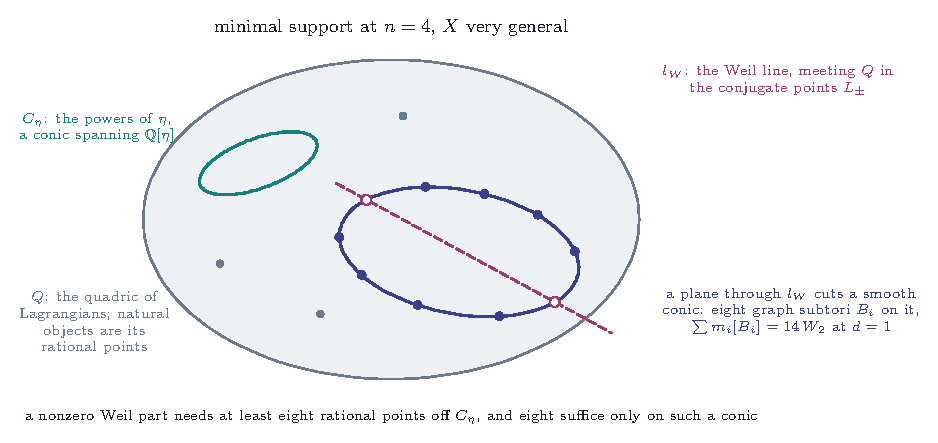
\includegraphics[width=0.94\textwidth]{fig_minimalsupport}
\caption{\Cref{thm:minimalsupport}. The quadric $Q$ of Lagrangians; the
rational points are the Chern characters of the natural objects on the split
member at $n=4$, up to the Veronese map $\nu_{4}$. The powers of the
polarisation fill the conic $C_{\eta}$ (teal), and the Weil line is spanned by
the conjugate points $L_{\pm}$ (open circles) in which the line $l_{W}$
(dashed) meets $Q$. A combination of natural characters with a nonzero Weil
part needs at least eight rational points off $C_{\eta}$, and with eight they
lie on one conic cut out by a plane through $l_{W}$ (indigo), such as the
eight graph subvarieties $B_{i}$ of \Cref{ex:fourteen}; the grey points are
natural objects off any such conic, which no relation of this size can use.}
\label{fig:minimalsupport}
\end{figure}

\begin{example}[Fourteen times a Weil class]\label{ex:fourteen}
Let $d=1$ and write $(\gamma-\sqrt{-1}\,\ell)^{4}=W_{1}+\sqrt{-1}\,W_{2}$ with
$W_{1},W_{2}$ rational, as in \cite[Theorem~15.2(iii)]{paperI}. The eight
subvarieties $B_{i}=B_{(p_{i},q_{i})}$ with
\[
  (p_{i},q_{i})=(1,-3),\,(1,-2),\,(1,2),\,(1,3),\,(2,-1),\,(2,1),\,(3,-1),\,(3,1)
\]
and $m=(-1,16,-16,1,-16,16,1,-1)$ satisfy
\[
  \textstyle\sum_{i}m_{i}[B_{i}]=14\,W_{2},
\]
with the sign of $\varphi$ for which $B_{(p,q)}$ has conormal forms
$p\xi_{j}-qx_{n+j}$ and $p\xi_{n+j}+qx_{j}$; with the opposite sign the right
side is $-14W_{2}$. Among the $12870$ sets of eight subvarieties with
$|p|,|q|\le3$ this one has the least $\sum_{i}m_{i}^{2}$, namely $1028$, and
the least $\sum_{i}|m_{i}|$, namely $68$. In
general the coefficients of the relation of \Cref{thm:minimalsupport} for eight
subvarieties are proportional to
$\bigl((q_{i}^{2}+dp_{i}^{2})\prod_{j\ne i}(p_{i}q_{j}-p_{j}q_{i})\bigr)^{-1}$.
The sum $E=\bigoplus_{i}\cO_{B_{i}}^{\oplus|m_{i}|}[k_{i}]\oplus\cO(\eta)
\oplus\cO(2\eta)\oplus\cO(3\eta)$, with $k_{i}=0$ for $m_{i}>0$ and $1$
otherwise, has $\ch(E)=14W_{2}+\sum_{k}c_{k}\eta^{k}$ with
$k!\,c_{k}=1+2^{k}+3^{k}$, so $\rho=3$ and $r=104$, while
$\dim\Ext^{2}(E,E)=28868$; by \Cref{cor:naturalsums} it is far from the
criterion, and every direct sum of natural objects with $N\ne0$ has
$\dim\Ext^{2}\ge8\cdot28=224$.
\end{example}

\begin{remark}[The flatness form for direct sums]\label{rem:flatsums}
\Cref{lem:p2primesummands} does not apply to the flatness form of
\Cref{prop:p2flat}, but a direct sum fails that form too when its
cross-extensions cannot interact. Let $E=\bigoplus_{i}(\cO_{B_{i}}\otimes
L_{i})^{\oplus m_{i}}[k_{i}]$ with the $B_{i}$ pairwise distinct abelian
subvarieties of dimension $n$ meeting pairwise in finite sets, such as the
$B_{(p,q)}$. The extensions between different summands are concentrated in
degree $n$, so an arrow of $\Ext^{1}$ between summands raises the shift by
$n-1$, and a chain of $a\ge1$ arrows lands in $\Ext^{2+a(n-1)}\ne\Ext^{2}$.
Every term of the Maurer--Cartan equation that involves a cross-extension
therefore lands in a zero group, the base $K_{E}$ is the product of the
varieties of commuting $2n$-tuples of $m_{i}\times m_{i}$ matrices with the
space of cross-extensions, and a count of dimensions, using the
simultaneously diagonalisable component, gives $\dim K_{E}>e-k$; so (ii) and
(iii) of \Cref{prop:p2flat} fail. We give this in outline only. Indecomposable objects,
among them iterated extensions of at least eight natural blocks, and sums
whose cross-extensions compose to nonzero classes are not covered.
\end{remark}
\section{Secant objects on the split member}\label{sec:secantobjects}

\subsection{Sums of line bundles and the positivity obstruction}
\label{ssec:whatobject}

\Cref{thm:semiregclosure} asks for one perfect complex at one base point.
The cheapest candidate is a sum of line bundles on a split member, because
there the Weil classes are already polynomials in $\beta$, $\widehat\beta$ and
$\ell$ by \cite[Theorem~15.2]{paperI}, so the Chern character one wants is
manifestly in reach. This subsection settles that candidate. It does not
exist, and the obstruction is not semiregularity: it is the Chern character
condition, and it fails because the norm form of $K$ is positive
definite.

The norm rules out three different constructions in this paper, by three
different mechanisms, and they should be kept apart.
\cite[Theorem~5.6]{paperI} uses the norm \emph{character} of $\Kx$ and an
equivariance hypothesis. \cite[Proposition~15.18]{paperI} uses the fact that the part $R$
of $H^{2}$ on which $\Kx$ acts through $\tau^{2}$ and $\bbar\tau^{\,2}$ has no
Hodge classes at a general point, which is a statement about the Hodge group.
\Cref{thm:positivity} below uses neither: it uses that $\Nm_{K/\QQ}$ is a
positive definite quadratic form on $K$ and that the multiplicities of a
filtration are positive integers. The three are independent, and only the
third is available at a special point, which is exactly where the object of
\Cref{prop:ktheory} has to live.

\begin{lemma}[The semiregularity map of a split object]\label{lem:splitsemireg}
Let $Y$ be a smooth projective complex variety and let
\[
  E=\bigoplus_{i=1}^{s}L_{i}[p_{i}]^{\oplus m_{i}},
  \qquad \lambda_{i}=c_{1}(L_{i}),
\]
with the $L_{i}$ line bundles, the $\lambda_{i}$ pairwise distinct and
$p_{i}\in\ZZ$. Then for $\zeta=(\zeta_{ij})\in\Ext^{2}(E,E)$,
\begin{equation}\label{eq:splitsigma}
  \sigma_{E}(\zeta)_{q}
  =\frac{1}{q!}\sum_{i=1}^{s}(-1)^{p_{i}}\,
    \mathrm{tr}(\zeta_{ii})\,\lambda_{i}^{\,q},
\end{equation}
so $\sigma_{E}$ annihilates $\Ext^{2}(L_{i}[p_{i}],L_{j}[p_{j}])$ for $i\ne j$
and the traceless part of each diagonal block. Consequently $\sigma_{E}$ is
injective if and only if all three of the following hold:
\begin{enumerate}[label=\textup{(\roman*)},nosep]
\item $m_{i}=1$ for every $i$;
\item $H^{\,2+p_{i}-p_{j}}\bigl(Y,L_{j}L_{i}^{-1}\bigr)=0$ for all $i\ne j$;
\item the map
  \[
    \Phi\colon H^{2}(\cO_{Y})^{\oplus s}\longrightarrow H^{*}(Y,\CC),
    \qquad
    (\zeta_{i})\longmapsto\sum_{i}e^{\lambda_{i}}\zeta_{i},
  \]
  is injective.
\end{enumerate}
\end{lemma}

\begin{proof}
The Atiyah class of a direct sum is the direct sum of the Atiyah classes, and
that of a line bundle is its first Chern class, so $\mathrm{At}(E)$ is
diagonal with entries $\lambda_{i}$ and $\mathrm{At}(E)^{q}$ is diagonal with
entries $\lambda_{i}^{\,q}$. The matrix product $\zeta\circ\mathrm{At}(E)^{q}$
therefore has $(i,j)$ entry $\zeta_{ij}\lambda_{i}^{\,q}$, and the trace keeps
only the diagonal; a shift by $p$ multiplies the trace by $(-1)^{p}$. That is
\eqref{eq:splitsigma}, and it exhibits the two spaces the map kills.

For the equivalence, the off-diagonal part of $\Ext^{2}(E,E)$ is
$\bigoplus_{i\ne j}\Ext^{2}(L_{i}[p_{i}],L_{j}[p_{j}])
=\bigoplus_{i\ne j}H^{2+p_{i}-p_{j}}(L_{j}L_{i}^{-1})$, which must vanish,
giving (ii); the diagonal block at $i$ is $H^{2}(\cO_{Y})\otimes
\mathrm{End}(\CC^{m_{i}})$ and only its trace survives, so $m_{i}=1$, giving
(i). What is left is $\bigoplus_{i}H^{2}(\cO_{Y})$, and by
\eqref{eq:splitsigma} an element $(\zeta_{i})$ of it dies exactly when
$\sum_{i}\lambda_{i}^{\,q}\zeta_{i}=0$ for every $q\ge0$, which is (iii) after
absorbing the signs $(-1)^{p_{i}}$ into the $\zeta_{i}$ and the factorials
into the grading.
\end{proof}

Condition (ii) is cheap, because the shifts $p_{i}$ are at our disposal: only
their parities are fixed by the Chern character, and a line bundle whose first
Chern class is nondegenerate of index $k$ has cohomology in degree $k$ alone,
so one may choose the $p_{i}$ to avoid every index that occurs. Condition
(iii) is a rank condition, and condition (i) is free. What is not free is the
Chern character itself, and that is the subject of the rest of this
subsection.

\begin{notation}[Coordinates on the divisor classes]\label{not:splitcoords}
Let $A_{0}=X\times\widehat{X}$ be a split member, $n\ge2$, and keep
$\gamma=d\beta-\widehat{\beta}$ from \cite[Notation~15.1]{paperI}. Write
\[
  \theta^{\pm}=\gamma\mp\sqrt{-d}\,\ell\in\textstyle\bigwedge^{2}V_{\pm},
  \qquad
  R_{0}=\QQ\gamma\oplus\QQ\ell\subset R .
\]
Every $\theta\in R_{0}$ is $\theta=u\theta^{+}+\bbar u\,\theta^{-}$ for a
unique $u\in K$, and in coordinates $u=g+h\sqrt{-d}$ corresponds to
$\theta=2g\gamma+2dh\,\ell$. By \cite[Proposition~15.19(iv)]{paperI} the group
$\NS(A_{0})_{\QQ}$ at a split member with $X$ general is
$\QQ\eta\oplus R_{0}$, so every divisor class $\lambda$ is $e\eta+\theta$ with
$e\in\QQ$ and $\theta\in R_{0}$, and we write $u(\lambda)\in K$ for the
coordinate of its $R_{0}$-part.
\end{notation}

\begin{lemma}[A basis in degree four]\label{lem:sixmonomials}
For $n\ge2$ the six products
$\beta^{2},\widehat\beta^{2},\ell^{2},\beta\widehat\beta,\beta\ell,
\widehat\beta\ell$
are linearly independent in $H^{4}(A_{0},\QQ)$. Equivalently the six classes
$\eta^{2}$, $\eta\theta^{+}$, $\eta\theta^{-}$, $(\theta^{+})^{2}$,
$(\theta^{-})^{2}$, $\theta^{+}\theta^{-}$ are a basis of the degree four part
of the subring generated by the divisor classes.
\end{lemma}

\begin{proof}
Grade $H^{*}(A_{0},\QQ)=\bigwedge^{*}U\otimes\bigwedge^{*}U^{\vee}$ by
bidegree. Then $\beta$ has bidegree $(2,0)$, $\widehat\beta$ has $(0,2)$ and
$\ell$ has $(1,1)$, so the six products have bidegrees $(4,0)$, $(0,4)$,
$(2,2)$, $(2,2)$, $(3,1)$, $(1,3)$. All are distinct except for the pair
$\beta\widehat\beta$ and $\ell^{2}$, and those two are independent in
$\bigwedge^{2}U\otimes\bigwedge^{2}U^{\vee}$ because
$\beta\widehat\beta=\beta\otimes\widehat\beta$ is decomposable there while
$\ell^{2}=-2\sum_{i<j}(x_{i}x_{j})\otimes(\xi_{i}\xi_{j})$ is diagonal in
the induced bases, of tensor rank $\binom{2n}{2}>1$. The second
description follows because the change of basis between the two sets of six
classes is invertible over $K$: $\eta=d\beta+\widehat\beta$ and
$\gamma=d\beta-\widehat\beta$ span the same plane as
$\beta$ and $\widehat\beta$ since $\det\begin{psmallmatrix}d&1\\
d&-1\end{psmallmatrix}=-2d\ne0$, and $\theta^{\pm}$ span the same plane
as $\gamma$ and $\ell$ over $\CC$.
\end{proof}

The next lemma says the same thing at every abelian variety of Weil type, not
only at a split member, and it says it without coordinates. It is the fact on
which the positivity argument turns.

\begin{lemma}[$\theta^{+}\theta^{-}$ is never proportional to $\eta^{2}$]
\label{lem:tensorrank}
Let $(A,\iota,\eta)$ be of $(K,-1,n)$-Weil type with $n\ge2$, and let
$0\ne\theta^{\pm}\in\bigwedge^{2}V_{\pm}$. Then $\theta^{+}\theta^{-}$ is not a
scalar multiple of $\eta^{2}$ in $H^{4}(A,\CC)$.
\end{lemma}

\begin{proof}
Both classes lie in the summand
$\bigwedge^{2}V_{+}\otimes\bigwedge^{2}V_{-}$ of $H^{4}(A,\CC)$, the isotypic
component for the character $\Nm^{2}$, so the question is one of tensor rank
there. The polarisation class $\eta$ lies in $V_{+}\otimes V_{-}$ and is the
hermitian form of \cite[Proposition~3.7]{paperI}, hence nondegenerate: in dual bases
$\eta=\sum_{a=1}^{2n}v_{a}\wedge w_{a}$ with $v_{a}$ a basis of $V_{+}$ and
$w_{a}$ a basis of $V_{-}$. Squaring,
\[
  \eta^{2}
  =\sum_{a,b}(v_{a}\wedge w_{a})(v_{b}\wedge w_{b})
  =-2\sum_{a<b}(v_{a}v_{b})\otimes(w_{a}w_{b}),
\]
which is diagonal in the induced bases of $\bigwedge^{2}V_{+}$ and
$\bigwedge^{2}V_{-}$ and therefore has tensor rank exactly $\binom{2n}{2}$.
The class $\theta^{+}\theta^{-}$ is, up to sign,
$\theta^{+}\otimes\theta^{-}$, of tensor rank one. For $n\ge2$ one has
$\binom{2n}{2}\ge6>1$, so the two cannot be proportional.
\end{proof}

\begin{theorem}[The positivity obstruction]\label{thm:positivity}
Let $(A,\iota,\eta)$ be of $(K,-1,n)$-Weil type with $n\ge2$, and suppose that
the only divisor classes on which $\Kx$ acts through the norm character are
the multiples of $\eta$, that is
\begin{equation}\label{eq:noextranorm}
  \NS(A)_{\QQ}\cap\bigl(V_{+}\otimes V_{-}\bigr)=\QQ\,\eta .
\end{equation}
Let $E$ be a perfect complex on $A$ whose Chern character is effective in the
exponential basis, meaning
\begin{equation}\label{eq:effectivech}
  \ch(E)=\sum_{i=1}^{s}m_{i}\,e^{\lambda_{i}},
  \qquad m_{i}\in\QQ_{>0},\quad\lambda_{i}\in\NS(A)_{\QQ},
\end{equation}
and write $\lambda_{i}=e_{i}\eta+\theta_{i}$ with $\theta_{i}$ in the part $R$
of $H^{2}(A,\QQ)$ carrying the characters $\tau^{2}$ and $\bbar\tau^{\,2}$, and
$u_{i}\in K$ for the $\theta^{+}$-coordinate of $\theta_{i}$. If $\ch_{2}(E)$
is a flat Hodge class, then
\begin{equation}\label{eq:normsum}
  \sum_{i=1}^{s}m_{i}\,\Nm_{K/\QQ}(u_{i})=0 ,
\end{equation}
and since $\Nm_{K/\QQ}$ is positive definite and every $m_{i}$ is positive,
$u_{i}=0$ for every $i$. Hence every $\lambda_{i}$ is a rational multiple of
$\eta$, and $\ch_{k}(E)\in\QQ\,\eta^{k}$ for every $k$. In particular
$\ch_{n}(E)$ has no component on the Weil line.
\end{theorem}

\begin{proof}
From \eqref{eq:effectivech},
$\ch_{2}(E)=\tfrac12\sum_{i}m_{i}\lambda_{i}^{2}$, and hypothesis
\eqref{eq:noextranorm} is what makes the decomposition
$\lambda_{i}=e_{i}\eta+\theta_{i}$ available with $e_{i}$ a scalar. Decompose
$H^{4}(A,\CC)$ into $\Kx$-isotypic pieces and keep the one for $\Nm^{2}$,
namely $\bigwedge^{2}V_{+}\otimes\bigwedge^{2}V_{-}$. Writing
$\theta_{i}=u_{i}\theta^{+}+\bbar u_{i}\theta^{-}$ for a fixed choice of
generators $\theta^{\pm}$ of $\bigwedge^{2}V_{\pm}$, one has
\[
  \lambda_{i}^{2}
  =e_{i}^{2}\eta^{2}
   +2e_{i}\eta\theta_{i}
   +u_{i}^{2}(\theta^{+})^{2}+\bbar u_{i}^{2}(\theta^{-})^{2}
   +2\Nm_{K/\QQ}(u_{i})\,\theta^{+}\theta^{-},
\]
and of these five terms only the first and the last are in the $\Nm^{2}$
piece: $\eta\theta_{i}$ carries $\Nm\tau^{2}$ and $\Nm\bbar\tau^{\,2}$, and
$(\theta^{\pm})^{2}$ carry $\tau^{4}$ and $\bbar\tau^{\,4}$, all four distinct
from $\Nm^{2}$. So the $\Nm^{2}$-part of $\ch_{2}(E)$ is
\[
  \tfrac12\Bigl(\sum_{i}m_{i}e_{i}^{2}\Bigr)\eta^{2}
  +\Bigl(\sum_{i}m_{i}\Nm_{K/\QQ}(u_{i})\Bigr)\theta^{+}\theta^{-}.
\]

Now compare with the flat Hodge classes of degree four. For $n\ge3$ they are
$\QQ\eta^{2}$ by \cite[Theorem~4.14]{paperI}. For $n=2$ they are
$\QQ\eta^{2}\oplus\HW(A)$, and $\HW(A)$ spans the summands for $\tau^{4}$ and
$\bbar\tau^{\,4}$, which are not $\Nm^{2}$. In both cases the $\Nm^{2}$-part
of a flat Hodge class of degree four is a multiple of $\eta^{2}$. By
\Cref{lem:tensorrank} the class $\theta^{+}\theta^{-}$ is not such a multiple,
so its coefficient must vanish, which is \eqref{eq:normsum}.

Finally $\Nm_{K/\QQ}(g+h\sqrt{-d})=g^{2}+dh^{2}$ with $d>0$, so
$\Nm_{K/\QQ}(u)\ge0$ with equality only at $u=0$, and a sum of nonnegative
terms with positive weights vanishes only when every term does. Then
$\ch_{k}(E)=\frac{1}{k!}\bigl(\sum_{i}m_{i}e_{i}^{k}\bigr)\eta^{k}$, and
$\eta^{k}$ is not on the Weil line by \cite[Theorem~4.14]{paperI}.
\end{proof}

\begin{corollary}[Objects filtered by line bundles]\label{cor:nofiltered}
Let $A$ satisfy \eqref{eq:noextranorm}, which holds at every split member of
\cite[Theorem~15.2]{paperI} and at every quaternionic base point of
\cite[Theorem~15.25]{paperI}. Then \Cref{thm:semiregclosure} cannot be applied at $A$
with any of the following:
\begin{enumerate}[label=\textup{(\alph*)},nosep]
\item a coherent sheaf admitting a filtration by line bundles, in particular
  any direct sum of line bundles;
\item a simple semi-homogeneous vector bundle in the sense of Mukai
  \cite{Muk78}, since such a bundle of rank $r$ has $\ch(E)=r\,e^{c_{1}(E)/r}$;
\item any iterated extension of the objects in (a) and (b).
\end{enumerate}
In each case the failure is not of the semiregularity hypothesis but of the
Chern character hypothesis of \Cref{prop:ktheory}: no such $E$ has a Chern
character which is a flat section of Hodge classes with a nonzero Weil
component.
\end{corollary}

\begin{proof}
First, \eqref{eq:noextranorm} holds at the points named. At a split member
$\NS(A)_{\QQ}$ has rank three with basis $\beta,\widehat\beta,\ell$ by
\cite[Proposition~15.19(iv)]{paperI}, and of these $\eta$ spans the norm-character part
while $\gamma$ and $\ell$ span $R$. At a quaternionic point $\NS(A)_{\QQ}$ is
the space of Rosati-symmetric elements of $B=(-d,b)_{\QQ}$, which is spanned
by $1$, $j$ and $ij$; the first gives $\eta$ and the other two are semilinear
over $K$, hence lie in $R$. In both cases the norm-character part of
$\NS(A)_{\QQ}$ is exactly $\QQ\eta$.

Each of (a), (b) and (c) has a Chern character of the shape
\eqref{eq:effectivech} with positive multiplicities, by additivity of $\ch$
along a filtration and by Mukai's computation of the Chern character of a
simple semi-homogeneous bundle. The conclusion of \Cref{thm:positivity} then
contradicts the requirement that $\ch_{n}(E)$ have a nonzero component on the
Weil line.
\end{proof}

\begin{remark}[Scope of the theorem, and the objects of
Markman]\label{rem:markmanpositivity}
At a very general member of the family $\NS(A)_{\QQ}=\QQ\eta$, so
\Cref{thm:positivity} is true for the empty reason that there are no
$\theta_{i}$ to begin with. Its content is at the special members, which is
exactly where \Cref{thm:semiregclosure} needs its object to live and where the
base points of \cite[Theorem~15.27]{paperI} are. That is the opposite of the usual
situation in this paper, where the special members are the easy ones.

The theorem does not touch the objects of Markman \cite{Mar25a,Mar25b}.
Those are sheaves whose class in $K_{0}$ is not a positive combination of
exponentials of divisor classes, so \eqref{eq:effectivech} fails for them at
the first step; and they live at very general points, where, as just noted,
the statement is vacuous. What the theorem does is remove the class of
objects one would reach for first, and it removes it for a reason which is
visible before any cohomology is computed.
\end{remark}

\begin{remark}[Signed sums of line bundles]
\label{rem:whatitmustbe}
\Cref{thm:positivity} uses positivity of the multiplicities and nothing else,
so it says exactly where to go next: the object must be a complex whose
class in $K_{0}$ is not effective, that is one in which the line bundles
appear with multiplicities of both signs. Such objects exist. Writing
$E=F\oplus G[1]$ with $F$ and $G$ sums of line bundles, the class in $K_{0}$
is $[F]-[G]$ and \eqref{eq:normsum} becomes
$\sum_{L_{i}\subset F}\Nm(u_{i})=\sum_{L_{j}\subset G}\Nm(u_{j})$, which is
satisfiable; and \Cref{lem:splitsemireg} still applies verbatim, with the
shifts absorbing condition (ii).

The object of \Cref{thm:semiregclosure}, if it exists at a split member, is
not a sum of line bundles in any arrangement of signs and shifts:
\Cref{cor:noline} below proves this in every dimension. It must have
$\Ext^{2}$ that the trace does not see, that is, it must be indecomposable in
the derived category. This description of the remaining construction is
sharper than the one in \Cref{rem:tworemain}.
\end{remark}

\subsection{An explicit object and the Prouhet--Tarry--Escott problem}
\label{ssec:pte}

\Cref{prop:ktheory} produces the object of \Cref{thm:semiregclosure} by an
existence argument: the Chern character is an isomorphism onto the Chow ring
with rational coefficients, so a $K$-theory class with the right character
exists. That is enough for the theorem and tells one nothing about the object.
This subsection writes it down. The answer turns the question into a
Diophantine one, and the Diophantine problem has a classical name.

\begin{setupenv}[Objects supported on $R$]\label{setup:pte}
Let $A$ be of $(K,-1,n)$-Weil type, $n\ge2$, satisfying
\eqref{eq:noextranorm}, and keep $\theta^{\pm}$ from
\Cref{not:splitcoords}. For $u\in K$ with $\theta(u)=u\theta^{+}+\bbar
u\,\theta^{-}\in\NS(A)_{\QQ}$, and for multiplicities $m_{i}\in\ZZ$, consider
\[
  v=\sum_{i=1}^{s}m_{i}\,e^{\theta(u_{i})},
  \qquad
  T_{q,r}=\sum_{i=1}^{s}m_{i}\,u_{i}^{q}\,\bbar u_{i}^{\,r}
  \quad (q,r\ge0).
\]
\end{setupenv}

\begin{proposition}[The Chern character in terms of the $u_{i}$]
\label{prop:chintermsofu}
In \Cref{setup:pte},
\begin{equation}\label{eq:chexpansion}
  v_{k}
  =\sum_{\substack{q+r=k\\ 0\le q,r\le n}}
    \frac{T_{q,r}}{q!\,r!}\,(\theta^{+})^{q}(\theta^{-})^{r},
\end{equation}
because $(\theta^{\pm})^{q}=0$ for $q>n$. Consequently $v$ is a flat section
of Hodge classes with a nonzero Weil component if
\begin{equation}\label{eq:pteconditions}
  T_{q,r}=0\ \ \text{for all } 0\le q,r\le n \text{ with }
  (q,r)\notin\{(0,0),(n,0),(0,n)\},
  \qquad T_{n,0}\ne0,
\end{equation}
and then $v_{0}=T_{0,0}=\sum_{i}m_{i}$, $v_{k}=0$ for $0<k<2n$ with $k\ne n$,
and
\[
  v_{n}=\frac{1}{n!}\Bigl(T_{n,0}(\theta^{+})^{n}
        +\bbar{T}_{n,0}(\theta^{-})^{n}\Bigr),
\]
a nonzero rational multiple of a generator of the Weil line, by
\cite[Theorem~15.2]{paperI}.
\end{proposition}

\begin{proof}
Expand $\theta(u_{i})^{k}$ by the binomial theorem, divide by $k!$ and collect;
the vanishing of $(\theta^{\pm})^{q}$ for $q>n$ is because
$\theta^{\pm}\in\bigwedge^{2}V_{\pm}$ and $\dim_{\CC}V_{\pm}=2n$. Under
\eqref{eq:pteconditions} the only surviving terms of \eqref{eq:chexpansion}
are the ones listed, and $(\theta^{+})^{n}$ spans $\bigwedge^{2n}V_{+}$, which
is the Weil line over $\CC$.
\end{proof}

So the search for the object of \Cref{thm:semiregclosure} is the search for a
finitely supported integer-valued function on $\cO_{K}$ that annihilates every
monomial $u^{q}\bbar u^{\,r}$ with $q,r\le n$ except three of them. Two things
follow at once, and they pull in opposite directions.

\begin{lemma}[Equal norms force the Prouhet--Tarry--Escott condition]
\label{lem:pte}
Suppose all the $u_{i}$ in \Cref{setup:pte} have the same norm
$N=\Nm_{K/\QQ}(u_{i})>0$. Then \eqref{eq:pteconditions} holds if and only if
\begin{equation}\label{eq:ptepure}
  \sum_{i}m_{i}u_{i}^{\,k}=0\ \ \text{for } k=0,1,\dots,n-1,
  \qquad
  \sum_{i}m_{i}u_{i}^{\,n}\ne0 .
\end{equation}
With $m_{i}=\pm1$ this says that the $u_{i}$ split into two multisets on the
circle $\Nm=N$ whose power sums agree through degree $n-1$ and differ at
degree $n$: a Prouhet--Tarry--Escott pair of degree $n-1$, constrained to a
norm circle of $\cO_{K}$.
\end{lemma}

\begin{proof}
For $q\ge r$ one has $u^{q}\bbar u^{\,r}=N^{r}u^{q-r}$, so
$T_{q,r}=N^{r}\sum_{i}m_{i}u_{i}^{\,q-r}$, and the pairs $(q,r)$ with
$q,r\le n$ realise every difference $k=q-r$ from $0$ to $n$. The excluded
pairs $(0,0)$ and $(n,0)$ are the ones with $r=0$ and $k=0$ or $k=n$; but
$k=0$ also occurs at $(1,1),\dots,(n,n)$, which are not excluded, so
$\sum_{i}m_{i}=0$ is still required. The remaining differences
$k=1,\dots,n-1$ each occur at some non-excluded pair, and $k=n$ occurs only at
$(n,0)$.
\end{proof}

\begin{theorem}[Equal norms cannot be semiregular]\label{thm:equalnorms}
Let $E=\bigoplus_{i}L_{i}[p_{i}]$ realise \eqref{eq:ptepure} with all norms
equal. Then $\ch_{0}(E)=0$, and the semiregularity map $\sigma_{E}$ has a
kernel of dimension at least $n^{2}$.
\end{theorem}

\begin{proof}
By \Cref{lem:pte} the case $k=0$ of \eqref{eq:ptepure} gives
$\sum_{i}m_{i}=0$, which is $\ch_{0}(E)$. For the kernel, take
$\zeta_{i}=m_{i}\zeta$ for a single $\zeta\in H^{2}(\cO_{A})$; then by
\Cref{lem:splitsemireg}(iii)
\[
  \Phi\bigl((m_{i}\zeta)_{i}\bigr)
  =\Bigl(\sum_{i}m_{i}e^{\lambda_{i}}\Bigr)\zeta=\ch(E)\,\zeta ,
\]
which by \Cref{prop:chintermsofu} is a multiple of $\omega\,\zeta$ with
$\omega$ a generator of the Weil line. Now $\HW(A)_{\CC}$ is spanned by
$\bigwedge^{2n}V_{+}$ and $\bigwedge^{2n}V_{-}$, and the Weil type condition
says $\dim V_{\pm}^{0,1}=n$; writing
$H^{2}(\cO_{A})=\bigwedge^{2}(V_{+}^{0,1}\oplus V_{-}^{0,1})$, the product of
a generator of $\bigwedge^{2n}V_{+}$ with $\zeta$ kills the components of
$\zeta$ in $\bigwedge^{2}V_{+}^{0,1}$ and in
$V_{+}^{0,1}\otimes V_{-}^{0,1}$, and likewise with the roles exchanged. So
$\omega\,\zeta=0$ for every $\zeta$ in
$V_{+}^{0,1}\otimes V_{-}^{0,1}$, a space of dimension $n^{2}$, and all of
those lie in the kernel of $\Phi$.
\end{proof}

\begin{corollary}[At least $n+1$ norms]\label{cor:nplusone}
If $E$ as in \Cref{setup:pte} satisfies \eqref{eq:pteconditions} and
$\ch_{0}(E)\ne0$, then the $u_{i}$ take at least $n+1$ distinct norms.
\end{corollary}

\begin{proof}
Let $N_{1},\dots,N_{\nu}$ be the distinct norms and $M_{j}$ the sum of the
$m_{i}$ over the level $\Nm(u_{i})=N_{j}$. The conditions $T_{r,r}=0$ for
$r=1,\dots,n$ read $\sum_{j}M_{j}N_{j}^{\,r}=0$ for $r=1,\dots,n$. The matrix
$(N_{j}^{\,r})_{1\le r\le n,\,1\le j\le\nu}$ has rank $\min(n,\nu)$ because the
$N_{j}$ are distinct and nonzero, so $\nu\le n$ forces every $M_{j}=0$ and
hence $\ch_{0}(E)=\sum_{j}M_{j}=0$.
\end{proof}

\subsubsection*{The smallest solution}

At $n=3$ and $K=\QQ(\sqrt{-3})$ the Prouhet--Tarry--Escott condition of
\Cref{lem:pte} has a particularly simple solution: the norm circle
$\Nm=1$ carries the six roots of unity of $K$, and the two cosets of the cube
roots of $-1$ and of $+1$ are a Prouhet--Tarry--Escott pair of degree
two. Explicitly, with $\zeta_{6}$ a primitive sixth root of unity, the
cube roots of $-1$ are $\zeta_{6},\zeta_{6}^{3},\zeta_{6}^{5}$ and those of
$+1$ are $1,\zeta_{6}^{2},\zeta_{6}^{4}$; each triple sums to zero and has
zero sum of squares,
while the sums of cubes are $-3$ and $+3$.

\begin{proposition}[An explicit object at $n=3$]\label{prop:explicitobject}
Let $K=\QQ(\sqrt{-3})$, $n=3$, and let $A_{0}=X\times\widehat X$ be a split
member. In the basis $\beta,\widehat\beta,\ell$ of $\NS(A_{0})_{\QQ}$ put
\[
  \lambda_{1}=(3,-1,3),\quad
  \lambda_{2}=(-6,2,0),\quad
  \lambda_{3}=(3,-1,-3),
\]
and $\lambda_{3+i}=-\lambda_{i}$ for $i=1,2,3$, with $m_{i}=+1$ for
$i\le3$ and $m_{i}=-1$ for $i\ge4$. Then the six classes are distinct and
integral, the perfect complex
\[
  E=\bigl(L_{1}\oplus L_{2}\oplus L_{3}\bigr)\ \oplus\
    \bigl(L_{4}\oplus L_{5}\oplus L_{6}\bigr)[3]
\]
has
\[
  \ch_{k}(E)=0\ \ (k\ne3),
  \qquad
  \ch_{3}(E)=12\,\omega_{1},
\]
and every difference $\lambda_{j}-\lambda_{i}$ with $i\ne j$ is nondegenerate
of index exactly $3$, so that conditions (i) and (ii) of
\Cref{lem:splitsemireg} hold for this shift. Condition (iii) fails: the map
$\Phi$ has rank $75$ instead of $90$, with kernel of dimension
$15=\dim H^{2}(\cO_{A_{0}})$.
\end{proposition}

\begin{proof}
With $d=3$, the class $\theta(u)=2g\gamma+6h\ell$ of $u=g+h\sqrt{-3}$ has
coordinates $(6g,-2g,6h)$, so $\lambda_{1},\lambda_{2},\lambda_{3}$ are the
images of the cube roots $\zeta_{6},\zeta_{6}^{3},\zeta_{6}^{5}$ of $-1$ and
$\lambda_{4},\lambda_{5},\lambda_{6}$ those of the cube roots of $+1$; the six
classes are distinct and integral. All six have norm $1$, and
$\sum_{i}m_{i}u_{i}^{k}$ is $0$ for $k=0,1,2$ and $-3-3=-6$ for $k=3$, so
\eqref{eq:ptepure} holds at $n=3$. By \Cref{lem:pte} and
\Cref{prop:chintermsofu}, $\ch_{k}(E)=0$ for $k\ne3$ and
$\ch_{3}(E)=-\bigl((\theta^{+})^{3}+(\theta^{-})^{3}\bigr)$, and by
\cite[Example~15.3]{paperI} at $n=3$,
$\omega_{1}\pm\sqrt{-3}\,\omega_{2}=-\frac16(\theta^{\mp})^{3}$; so
$\ch_{3}(E)=12\,\omega_{1}$.

Every difference is $\lambda_{j}-\lambda_{i}=\theta(w)$ with
$w=u_{j}-u_{i}\ne0$, and $\theta(w)$ is nondegenerate of index $n$ for every
$w\in K^{\times}$. Indeed $\theta(1)=2\gamma$ and $\theta(\sqrt{-d})=2d\ell$ are of
type $(1,1)$, hence so are $\theta^{\pm}$, so
$\theta^{+}\in V_{+}^{1,0}\otimes V_{+}^{0,1}$, and $V_{+}^{0,1}$ is the
conjugate of $V_{-}^{1,0}$. In the splitting of the tangent space dual to
$H^{1,0}=V_{+}^{1,0}\oplus V_{-}^{1,0}$, the hermitian form of $\theta(w)$
therefore has the block form
$\bigl(\begin{smallmatrix}0&wP\\ \bar wP^{*}&0\end{smallmatrix}\bigr)$, with $P$
the block of $2\gamma$, which is invertible because $\gamma$ is nondegenerate.
Its eigenvalues are plus and minus the singular values of $wP$, so it has
signature $(n,n)$, and a line bundle with this class has cohomology only in
degree $n$ \cite[Chapter~3]{BL04}. For the shift, condition (ii) asks that
$2+p_{i}-p_{j}\ne3$ whenever $i\ne j$, that is $p_{i}-p_{j}\ne1$; within each
of the two blocks the difference is $0$, and between them it is $\pm3$.

For the rank, the $u_{i}$ are the six sixth roots of unity, each once, and
$\bbar u_{i}=u_{i}^{-1}$. Absorb the signs into the $\zeta_{i}$ as in
\Cref{lem:splitsemireg}(iii) and expand
$e^{\lambda_{i}}=e^{u_{i}\theta^{+}}e^{\bbar u_{i}\theta^{-}}$:
\[
  \Phi(\zeta)=\sum_{a,b=0}^{3}\frac{(\theta^{+})^{a}(\theta^{-})^{b}}{a!\,b!}\,Z_{a-b},
  \qquad Z_{k}=\sum_{i}u_{i}^{k}\zeta_{i},
\]
with $k$ read modulo $6$. The $Z_{0},\dots,Z_{5}$ determine the $\zeta_{i}$,
by a Vandermonde matrix. Split
$H^{0,2}(A_{0})=\bigwedge^{2}V_{+}^{0,1}\oplus(V_{+}^{0,1}\otimes V_{-}^{0,1})
\oplus\bigwedge^{2}V_{-}^{0,1}$, write $Z_{k}=Z_{k}^{+}+Z_{k}^{0}+Z_{k}^{-}$
accordingly, and grade $H^{*}(A_{0})=\bigwedge^{*}V_{+}\otimes\bigwedge^{*}V_{-}$
by the Hodge types of the two factors. The term
$(\theta^{+})^{a}(\theta^{-})^{b}Z_{k}^{0}$ has types $(a,a+1)$ and $(b,b+1)$,
the term with $Z_{k}^{+}$ has types $(a,a+2)$ and $(b,b)$, and the term with
$Z_{k}^{-}$ has types $(a,a)$ and $(b,b+2)$. These are different for
different $(a,b)$ and different pieces, so every term vanishes separately.
Since $\theta^{\pm}$ pairs $V_{\pm}^{1,0}$ nondegenerately with $V_{\pm}^{0,1}$,
both of dimension $3$, multiplication by $(\theta^{\pm})^{a}$ is injective on
$\bigwedge^{j}V_{\pm}^{0,1}$ when $a+j\le3$ and zero otherwise; in bases
with $\theta^{+}=\sum_{i}e_{i}f_{i}$ it sends $f_{J}$ to a signed sum of the
$e_{I}f_{I\cup J}$ with $I\cap J=\emptyset$, $|I|=a$, and different $J$ give
disjoint supports. Hence $Z_{k}^{0}=0$ unless no $a,b\le2$ have $a-b\equiv k$,
which leaves $k=3$; $Z_{k}^{+}=0$ unless no $a\le1$, $b\le3$ have
$a-b\equiv k$, which leaves $k=2$; and likewise $Z_{k}^{-}=0$ unless $k=4$. So
$\ker\Phi$ is $V_{+}^{0,1}\otimes V_{-}^{0,1}$ at $k=3$ together with
$\bigwedge^{2}V_{+}^{0,1}$ at $k=2$ and $\bigwedge^{2}V_{-}^{0,1}$ at $k=4$, of
dimension $9+3+3=15=\dim H^{2}(\cO_{A_{0}})$, and $\Phi$ has rank
$90-15=75$. The first summand is the kernel of \Cref{thm:equalnorms}.
\end{proof}

\begin{remark}[What the construction settles]\label{rem:pteoutcome}
Three things are settled. The object of \Cref{prop:ktheory} is not an
abstraction: at $n=3$ over $\QQ(\sqrt{-3})$ it is six line bundles and a
shift, and its Chern character is exactly $12$ times a Weil class with every
other graded piece zero. The construction is completely general, and
\Cref{lem:pte} identifies the constraint as a Prouhet--Tarry--Escott problem
on a norm circle, a question of a kind that can be attacked directly. And
\Cref{cor:nplusone} says what any semiregular solution must look like: the
$u_{i}$ must take at least $n+1$ distinct norms, because otherwise the rank is
zero and the argument of \Cref{thm:equalnorms} produces a kernel of
dimension $n^{2}$.

This leaves the existence of a solution with $n+1$ norms. The level sums are
then forced up to scale (\Cref{thm:pterange}), and \Cref{cor:noline} shows
that no solution could serve, because a line bundle summand off the
polarisation line is obstructed along the family whatever the norms.
\end{remark}

\subsubsection*{The obstruction classes of the explicit object}

\cite[Corollary~9.18]{paperI} and \cite[Remark~9.21]{paperI} say that the kernel of
$\sigma_{E}$ contains a copy of the tangent space of the Weil family, and
that this is a statement about where the semiregularity map is blind, not a
statement that the object is obstructed. For the explicit object the
obstruction classes can be written down, and they are not zero. The
computation is elementary and we record it in general.

Recall the conventions of \cite[Section~9.3]{paperI}: a first-order deformation of
$A$ is $v\in\Hom(H^{1,0},H^{0,1})=H^{1}(A,T_{A})$, extended by zero on
$H^{0,1}$ and acting on $H^{*}(A,\CC)$ as a derivation $v\lrcorner$; a class
$\xi$ of type $(p,p)$ stays of type $(p,p)$ to first order along $v$ exactly
when $v\lrcorner\,\xi=0$. For a line bundle $L$ with $\lambda=c_{1}(L)$ the
Atiyah class is $\lambda\in H^{1}(\Omega^{1}_{A})$, its contraction with $v$
is $v\lrcorner\,\lambda\in H^{2}(\cO_{A})=H^{0,2}(A)$, and this is the
obstruction to deforming $L$ along $v$; a shift does not change it. For
$E=\bigoplus_{i}L_{i}[p_{i}]$ the Atiyah class is diagonal with entries
$\lambda_{i}$, as in the proof of \Cref{lem:splitsemireg}, so the
obstruction to deforming $E$ along $v$ is the diagonal element
\begin{equation}\label{eq:obdef}
  \ob_{E}(v)=\bigl(v\lrcorner\,\lambda_{i}\bigr)_{i}
  \in\bigoplus_{i}H^{0,2}(A)\subset\Ext^{2}(E,E).
\end{equation}

\begin{proposition}[The obstruction map of a split object]
\label{prop:splitobstruction}
Let $A_{0}=X\times\widehat X$ be a split member with $\beta$ principal and
$X$ general, so that $\NS(A_{0})_{\QQ}=\langle\beta,\widehat\beta,\ell\rangle$
by \cite[Proposition~15.19(iv)]{paperI}. Let $T=T_{[A_{0}]}\cD_{n,n}$ be the space of
polarised first-order deformations commuting with $K$, of dimension $n^{2}$
by \cite[Proposition~9.14]{paperI}, and put
\[
  T_{\mathrm{spl}}
  =\bigl\{\,v\in\Hom(H^{1,0},H^{0,1})\;:\;
    v\lrcorner\,\beta=v\lrcorner\,\widehat\beta=v\lrcorner\,\ell=0\,\bigr\}.
\]
Let $E=\bigoplus_{i=1}^{s}L_{i}[p_{i}]$ with $\lambda_{i}=c_{1}(L_{i})$ and
let $\ob_{E}\colon T\to\bigoplus_{i}H^{0,2}(A_{0})$ be the map
\eqref{eq:obdef} restricted to $T$.
\begin{enumerate}[label=\textup{(\roman*)},nosep]
\item $T_{\mathrm{spl}}$ is the tangent space to the split locus: it has
  dimension $n(n+1)/2$, it is contained in $T$, and it consists of the
  deformations of $X\times\widehat X$ induced by the polarised deformations
  of $(X,\beta)$.
\item If the classes $\lambda_{i}$ together with $\eta$ span
  $\NS(A_{0})_{\QQ}$, then $\ker\ob_{E}=T_{\mathrm{spl}}$ and
  $\operatorname{rank}\ob_{E}=n(n-1)/2$, the codimension of the split locus
  in $\cD_{n,n}$.
\item If $\ch_{k}(E)\in\QQ\eta^{k}$ for $k\ne n$ and
  $\ch_{n}(E)\in\QQ\eta^{n}\oplus\HW(A_{0})$, then
  $\sigma_{E}\circ\ob_{E}=0$ on $T$: for every $v\in T$,
  \begin{equation}\label{eq:sigmaob}
    \sigma_{E}\bigl(\ob_{E}(v)\bigr)=v\lrcorner\,\ch(E)=0 .
  \end{equation}
\item For the object of \Cref{prop:explicitobject}, at $n=3$ and
  $K=\QQ(\sqrt{-3})$: $\ker\ob_{E}=T_{\mathrm{spl}}$ has dimension $6$ and
  $\ob_{E}$ has rank $3$; the image of $\ob_{E}$ lies in $\ker\sigma_{E}$;
  the subspace $\Delta=\{z\cdot\id_{E}:z\in\Ann_{H^{0,2}}(\omega_{1})\}$ of
  \cite[Corollary~9.18]{paperI} has dimension $9$ and meets the image of $\ob_{E}$
  only in zero, so that $\Delta\oplus\image\ob_{E}$ is a twelve-dimensional
  subspace of the fifteen-dimensional kernel of $\sigma_{E}$; and
  $\ob_{E}(v)$ has components $v\lrcorner\,\lambda_{i}$ on $L_{i}$ and
  $-v\lrcorner\,\lambda_{i}$ on $L_{i}^{-1}[3]$, so it lies on the line of
  vectors of the shape $(z,\dots,z)$ only when it vanishes. In particular
  $E$ has a nonzero first-order obstruction along every $v\in T$ not tangent
  to the split locus, and no element $z\cdot\id_{E}$ of $\Ext^{2}(E,E)$
  cancels it.
\end{enumerate}
\end{proposition}

\begin{proof}
(i) Let $P=H^{1,0}(X)\subset H^{1}(X,\CC)=U^{\vee}_{\CC}$ with basis
$p_{1},\dots,p_{n}$, so that $p_{1},\dots,p_{n},\bbar p_{1},\dots,\bbar p_{n}$
is a basis of $U^{\vee}_{\CC}$, and let $q_{a},\bbar q_{a}$ be the dual basis
of $U_{\CC}=H^{1}(\widehat X,\CC)$; the dual of a conjugate basis is the
conjugate of the dual basis, so the notation is consistent. The Poincar\'e
class is the identity element of $U^{\vee}\otimes U$,
\[
  \ell=\sum_{a=1}^{n}\bigl(p_{a}\wedge q_{a}+\bbar p_{a}\wedge\bbar q_{a}\bigr),
\]
and it is of type $(1,1)$, which forces $H^{1,0}(\widehat X)=\langle\bbar
q_{a}\rangle$ and $H^{0,1}(\widehat X)=\langle q_{a}\rangle$: the Hodge
structure of $\widehat X$ is the dual one. Since $\beta$ is of type $(1,1)$
and nondegenerate, $\beta=\sum_{a,b}h_{ab}\,p_{a}\wedge\bbar p_{b}$ with
$h\in\GL_{n}(\CC)$; and since $\beta$ is principal with Gram matrix $B$ in a
symplectic basis of $U$ and $\widehat\beta$ has Gram matrix $-B^{-1}=B$ in
the dual basis of $U^{\vee}$, the Gram matrix of $\widehat\beta$ in the
basis $p_{a},\bbar p_{a}$ is minus the inverse of the Gram matrix
$\begin{psmallmatrix}0&h\\-h^{\top}&0\end{psmallmatrix}$ of $\beta$ in the
basis $q_{a},\bbar q_{a}$, which gives
$\widehat\beta=-\sum_{a,b}(h^{-1})_{ab}\,\bbar q_{a}\wedge q_{b}$.

Now $H^{1,0}(A_{0})=\langle p_{a}\rangle\oplus\langle\bbar q_{a}\rangle$ and
$H^{0,1}(A_{0})=\langle\bbar p_{a}\rangle\oplus\langle q_{a}\rangle$, so a
deformation $v$ is four $n\times n$ matrices,
\[
  v(p_{a})=\sum_{c}\bigl(A_{ca}\,\bbar p_{c}+C_{ca}\,q_{c}\bigr),
  \qquad
  v(\bbar q_{a})=\sum_{c}\bigl(B_{ca}\,\bbar p_{c}+D_{ca}\,q_{c}\bigr),
\]
and $v$ kills $\bbar p_{a}$ and $q_{a}$. Contracting,
\[
  v\lrcorner\,\ell
  =\sum_{a,c}\Bigl(A_{ca}\,\bbar p_{c}\wedge q_{a}+C_{ca}\,q_{c}\wedge q_{a}
   +B_{ca}\,\bbar p_{a}\wedge\bbar p_{c}+D_{ca}\,\bbar p_{a}\wedge q_{c}\Bigr),
\]
and reading off the three kinds of monomials, $v\lrcorner\,\ell=0$ if and only
if $D=-A^{\top}$ and $B$, $C$ are symmetric. Next
\[
  v\lrcorner\,\beta
  =\sum_{a,b,c}h_{ab}\Bigl(A_{ca}\,\bbar p_{c}\wedge\bbar p_{b}
   +C_{ca}\,q_{c}\wedge\bbar p_{b}\Bigr),
\]
so $v\lrcorner\,\beta=0$ if and only if $Ch=0$, that is $C=0$, and $Ah$ is
symmetric. Likewise $v\lrcorner\,\widehat\beta=0$ if and only if $B=0$ and
$Dh^{-1}$ is symmetric. Given $D=-A^{\top}$, the last condition reads
$A^{\top}h^{-1}=h^{-\top}A$, which after multiplication by $h^{\top}$ on the
left and by $h$ on the right is $h^{\top}A^{\top}=Ah$, the symmetry of $Ah$
again. Hence
\[
  T_{\mathrm{spl}}=\bigl\{(A,B,C,D)=(A,0,0,-A^{\top})\;:\;Ah\ \text{symmetric}\bigr\},
\]
of dimension $n(n+1)/2$. It is the tangent space to the split locus: the
same computation on $X$ alone shows that the polarised first-order
deformations of $(X,\beta)$ are the matrices $A$ with $Ah$ symmetric, the
space $T_{[X]}\cA_{n}$ of dimension $n(n+1)/2$; the deformation of
$\widehat X$ induced by $A$ is the dual one, $-A^{\top}$; and the map
$A\mapsto(A,0,0,-A^{\top})$ is injective. Finally $T_{\mathrm{spl}}\subseteq
T$: for $v\in T_{\mathrm{spl}}$, $v\lrcorner\,\eta=0$ because
$\eta\in\langle\beta,\widehat\beta\rangle$, so $v$ is polarised, and
$v\lrcorner\,\omega_{1}=v\lrcorner\,\omega_{2}=0$ because $\omega_{1}$ and
$\omega_{2}$ are polynomials in $\beta,\widehat\beta,\ell$ by
\cite[Theorem~15.2]{paperI} and $v\lrcorner$ is a derivation; by
\cite[Proposition~9.14]{paperI} such a $v$ commutes with $K$.

(ii) Every $v\in T$ has $v\lrcorner\,\eta=0$. If the $\lambda_{i}$ and
$\eta$ span $\NS(A_{0})_{\QQ}=\langle\beta,\widehat\beta,\ell\rangle$, then
$v\lrcorner\,\lambda_{i}=0$ for all $i$ is equivalent, for $v\in T$, to
$v\lrcorner\,\beta=v\lrcorner\,\widehat\beta=v\lrcorner\,\ell=0$, so
$\ker\ob_{E}=T\cap T_{\mathrm{spl}}=T_{\mathrm{spl}}$ by (i), and the rank
is $n^{2}-n(n+1)/2=n(n-1)/2$, which is the codimension of
\cite[Proposition~15.19(iii)]{paperI}.

(iii) By \eqref{eq:splitsigma}, $\sigma_{E}(\zeta)=\sum_{i}(-1)^{p_{i}}
\zeta_{ii}\,e^{\lambda_{i}}$ for a diagonal $\zeta$. Since $v\lrcorner$ is a
derivation and $v\lrcorner\,\lambda_{i}$ has even degree,
$v\lrcorner\,\lambda_{i}^{\,q}=q\,\lambda_{i}^{\,q-1}(v\lrcorner\,\lambda_{i})$
and so $v\lrcorner\,e^{\lambda_{i}}=(v\lrcorner\,\lambda_{i})\,e^{\lambda_{i}}$.
Therefore
\[
  \sigma_{E}\bigl(\ob_{E}(v)\bigr)
  =\sum_{i}(-1)^{p_{i}}(v\lrcorner\,\lambda_{i})\,e^{\lambda_{i}}
  =v\lrcorner\sum_{i}(-1)^{p_{i}}e^{\lambda_{i}}
  =v\lrcorner\,\ch(E).
\]
For $v\in T$ one has $v\lrcorner\,\eta^{k}=k\eta^{k-1}(v\lrcorner\,\eta)=0$,
and $v\lrcorner\,\omega=0$ for every $\omega\in\HW(A_{0})$ by
\cite[Proposition~9.14]{paperI}; under the hypothesis on $\ch(E)$ this gives
\eqref{eq:sigmaob}.

(iv) The three classes $\lambda_{1}=\gamma+3\ell$, $\lambda_{2}=-2\gamma$,
$\lambda_{3}=\gamma-3\ell$ span $\langle\gamma,\ell\rangle$, and
$\langle\eta,\gamma\rangle=\langle\beta,\widehat\beta\rangle$ by the
determinant in the proof of \Cref{lem:sixmonomials}, so (ii) applies and
gives the kernel and the rank; \Cref{prop:explicitobject} gives the
hypothesis of (iii), so the image lies in $\ker\sigma_{E}$. The subspace
$\Delta$ has dimension $\dim\Ann_{H^{0,2}}(\omega_{1})=n^{2}=9$ by
\cite[Lemma~9.6]{paperI}. The components of $\ob_{E}(v)$ on $L_{i}$ and on
$L_{i}^{-1}[3]$ are $v\lrcorner\,\lambda_{i}$ and
$v\lrcorner\,(-\lambda_{i})=-v\lrcorner\,\lambda_{i}$, so an element of the
image of the shape $(z,\dots,z)$ has $z=-z$, hence is zero; this is
$\Delta\cap\image\ob_{E}=0$, and with $\dim\ker\sigma_{E}=15$ from
\Cref{prop:explicitobject} the dimension count follows.
\end{proof}

\begin{remark}[Meaning of the obstruction classes]\label{rem:obstructionmeaning}
\Cref{prop:splitobstruction} sharpens \cite[Remark~9.21]{paperI} in one
respect and exposes a limit of the criterion in another. First, for the
explicit object the obstruction classes along the family are nonzero, and
they are nonzero exactly in the $n(n-1)/2$ directions normal to the split
locus, which are the directions in which the Weil class has to be
transported. Second, those classes lie in the kernel of $\sigma_{E}$ by
\eqref{eq:sigmaob}, and \eqref{eq:sigmaob} holds for every object whose
Chern character is a flat section of Hodge classes along the family, so the
semiregularity map cannot detect the obstruction of any such object. The
obstruction is therefore nonzero, and the criterion cannot see it. For
the explicit object the
situation is the worst possible: the twelve dimensions
$\Delta\oplus\image\ob_{E}$ of the kernel are accounted for by the two
mechanisms of \cite[Corollary~9.18]{paperI} and \eqref{eq:obdef}, the remaining
three lie on the even side of \cite[Corollary~9.8]{paperI} as well, and none of
the fifteen is an artefact. The classes of the shape $z\cdot\id_{E}$ are the
ones a change of the twisting class would contribute, one and the same $z$
to every rank one summand; the last assertion of (iv) says that no such
change removes the obstruction. So the explicit object does not move off the
split locus to first order, either as a complex or as a twisted complex, and
the question of \cite[Question~15.13]{paperI} for it is not one of verifying a
hypothesis but of replacing the object.

The positive content is a recipe. By (ii), a split object whose classes
span $\NS(A_{0})_{\QQ}$ with $\eta$ has obstruction map of rank
$n(n-1)/2$ against the family, and the spanning hypothesis is more than is
needed: a single class $\theta\in\NS(A_{0})_{\QQ}$ not proportional to
$\eta$ already has $\{v\in T:v\lrcorner\,\theta=0\}=T_{\mathrm{spl}}$.
Indeed, every $v\in T$ kills $\eta$ and commutes with $K$, so it is a pair
$(v_{+},v_{-})$ with $v_{\pm}\in\Hom(V_{\pm}^{1,0},V_{\pm}^{0,1})$. Since
$\theta^{\pm}$ is of type $(1,1)$ in $\bigwedge^{2}V_{\pm}$, the $R_{0}$-part
$u\theta^{+}+\bbar u\,\theta^{-}$ of $\theta$, with $u\ne0$, gives
$v\lrcorner\,\theta=u\,v_{+}\lrcorner\,\theta^{+}+\bbar u\,v_{-}\lrcorner\,\theta^{-}$,
whose two terms lie in the different summands $\bigwedge^{2}V_{+}^{0,1}$ and
$\bigwedge^{2}V_{-}^{0,1}$ of $H^{0,2}(A_{0})$. So the kernel of
$v\mapsto v\lrcorner\,\theta$ on $T$ does not depend on $u\ne0$; it is
therefore the common kernel for $\gamma$ and $\ell$, the cases $u=1$ and
$u=\sqrt{-d}$, which is $T_{\mathrm{spl}}$ by (ii). So every split object built from line bundles
other than powers of $\eta$ is obstructed in exactly the normal directions
to the split locus, and \Cref{thm:positivity} says that an object built
from powers of $\eta$ carries no Weil class. What survives is the statement
of \cite[Remark~9.9]{paperI}: the object must have positive rank.
\end{remark}

\subsubsection*{The evaluation map of the explicit object}

\cite[Theorem~9.19]{paperI} places the copy $\Delta$ of the tangent space inside the
image of the evaluation map. For a split object the whole of
$\operatorname{ev}_{E}$ can be written down, and for the explicit object the
entire kernel of $\sigma_{E}$ turns out to lie in its image. We identify
$HH^{2}(A_{0})$ with
\begin{equation}\label{eq:HT2}
  HT^{2}(A_{0})
  =H^{0,2}(A_{0})\;\oplus\;\Hom\bigl(H^{1,0},H^{0,1}\bigr)\;\oplus\;
   \textstyle\bigwedge^{2}\bigl(H^{1,0}\bigr)^{\vee}
\end{equation}
by the Hochschild--Kostant--Rosenberg isomorphism, the three summands being
$H^{2}(\cO)$, $H^{1}(T)$ and $H^{0}(\bigwedge^{2}T)$ for the trivial tangent
bundle. An element $x=(z,v,\pi)$ acts on $H^{*}(A_{0},\CC)$ by $z\wedge$, by
the derivation $v\lrcorner$ of \cite[Section~9.3]{paperI}, and by the double
contraction $\pi\lrcorner$, which removes two $(1,0)$ slots; we write
$x\lrcorner\,\xi$ for the sum of the three.

The double contraction is a second order operator. For a class $\lambda$ of
type $(1,1)$, which has a single $(1,0)$ slot, $\pi\lrcorner\,\lambda=0$ and
$\pi\lrcorner\,\lambda^{k}=\binom{k}{2}\lambda^{k-2}\,(\pi\lrcorner\,\lambda^{2})$,
because $\pi\lrcorner$ is a composite of two interior products, each of which
is an antiderivation, and the only nonzero terms are those in which the two
interior products hit two different factors. Summing over $k$ with the
factorials gives
$\pi\lrcorner\,e^{\lambda}=\tfrac12(\pi\lrcorner\,\lambda^{2})\,e^{\lambda}$,
exactly parallel to $v\lrcorner\,e^{\lambda}=(v\lrcorner\,\lambda)\,e^{\lambda}$
for the first order operator $v\lrcorner$. This is the whole content of the
compatibility \eqref{eq:sigmaev} below: the semiregularity map of a line
bundle is multiplication by $e^{\lambda}$, and every summand of $HT^{2}$ acts
on $e^{\lambda}$ as multiplication by a class in $H^{0,2}$ which is precisely
the value of $\operatorname{ev}_{L}$. The same identity, for arbitrary $E$, is
the commutative square of Buchweitz and Flenner \cite[Corollary 4.3]{BF03} and
its Hochschild form in \cite[Lemma 11.3]{Mar25b}; on an abelian variety the
Todd class is trivial and no correction to the HKR map is needed
\cite{Cal05,BF08}.

\begin{proposition}[The evaluation map of a split object]\label{prop:evaluation}
Let $A_{0}$ be a split member with $X$ general and let
$E=\bigoplus_{i=1}^{s}L_{i}[p_{i}]$ with $\lambda_{i}=c_{1}(L_{i})$ and all
$\Ext^{2}(L_{i}[p_{i}],L_{j}[p_{j}])$, $i\ne j$, zero, so that
$\Ext^{2}(E,E)=\bigoplus_{i}H^{0,2}(A_{0})$.
\begin{enumerate}[label=\textup{(\roman*)},nosep]
\item Under \eqref{eq:HT2}, $\operatorname{ev}_{E}$ is diagonal:
  \begin{equation}\label{eq:evsplit}
    \operatorname{ev}_{E}(z,v,\pi)_{i}
    =z+v\lrcorner\,\lambda_{i}+\tfrac12\,\pi\lrcorner\,\lambda_{i}^{2}
    \;\in\;H^{0,2}(A_{0})=\Ext^{2}\bigl(L_{i}[p_{i}],L_{i}[p_{i}]\bigr).
  \end{equation}
\item For every $x\in HT^{2}(A_{0})$,
  \begin{equation}\label{eq:sigmaev}
    \sigma_{E}\bigl(\operatorname{ev}_{E}(x)\bigr)=x\lrcorner\,\ch(E),
  \end{equation}
  and consequently
  $\ker\sigma_{E}\cap\image\operatorname{ev}_{E}
   =\operatorname{ev}_{E}\bigl(\{x:x\lrcorner\,\ch(E)=0\}\bigr)$.
  The weakened hypothesis of \cite[Question 11.4]{Mar25b} holds for $E$ if
  and only if $\operatorname{ev}_{E}$ kills every $x$ that preserves
  $\ch(E)$ to first order.
\item $\dim HT^{2}(A_{0})=2\binom{2n}{2}+4n^{2}$ and
  $\dim\Ext^{2}(E,E)=s\binom{2n}{2}$; for $s\ge5$ and every $n\ge2$ the
  second exceeds the first, so $\operatorname{ev}_{E}$ is not surjective and
  \cite[Lemma 11.3]{Mar25b} cannot apply to a sum of five or more line
  bundles.
\item For the object of \Cref{prop:explicitobject}, with
  $\lambda_{i}=u_{i}\theta^{+}+\bbar u_{i}\theta^{-}$ as in
  \Cref{not:splitcoords}: the space $\{x:x\lrcorner\,\ch(E)=0\}$ is
  $\Ann_{H^{0,2}}(\omega_{1})\oplus\{v:v\lrcorner\,\omega_{1}=0\}\oplus
  \{\pi:\pi\lrcorner\,\omega_{1}=0\}$, of dimensions $9$, $18$ and $9$; the
  first and the third summands are both carried by $\operatorname{ev}_{E}$
  onto $\Delta$; the second is carried onto
  \[
    \Sigma=\bigl\{\,(u_{i}a+\bbar u_{i}b)_{i=1}^{6}\;:\;
      a\in\textstyle\bigwedge^{2}V_{+}^{0,1},\ b\in\bigwedge^{2}V_{-}^{0,1}\,\bigr\},
    \qquad \dim\Sigma=n(n-1)=6,
  \]
  which contains the image of the obstruction map of
  \Cref{prop:splitobstruction}; $\Delta\cap\Sigma=0$; and
  \[
    \ker\sigma_{E}=\Delta\oplus\Sigma\subseteq\image\operatorname{ev}_{E}.
  \]
  So every direction in which $\sigma_{E}$ is blind is the value of
  $\operatorname{ev}_{E}$ on a Hochschild class that preserves $\ch(E)$ to
  first order, and the weakened hypothesis fails for $E$ by all fifteen
  dimensions. The rank of $\operatorname{ev}_{E}$ is $45$.
\end{enumerate}
\end{proposition}

\begin{proof}
(i) The evaluation map is the action of $HH^{*}(A_{0})$ on
$\Ext^{*}(E,E)$, which under HKR is contraction of a polyvector in
$H^{q}(\bigwedge^{p}T)$ with $\tfrac{1}{p!}\mathrm{At}(E)^{p}$
\cite{BF08}; for $p=0$ this is $z\cdot\id_{E}$ as in the proof of
\cite[Theorem~9.19]{paperI}, for $p=1$ it is $v\lrcorner\,\mathrm{At}(E)$, the map
\eqref{eq:obdef}, and for $p=2$ it is $\tfrac12\pi\lrcorner\,\mathrm{At}(E)^{2}$.
The Atiyah class of $E$ is diagonal with entries $\lambda_{i}$, so all three
are diagonal with the entries displayed.

(ii) By \eqref{eq:splitsigma}, $\sigma_{E}(\zeta)=\sum_{i}(-1)^{p_{i}}\zeta_{i}
e^{\lambda_{i}}$ for diagonal $\zeta$. The three terms of \eqref{eq:evsplit}
are exactly the factors by which $z\wedge$, $v\lrcorner$ and $\pi\lrcorner$
multiply $e^{\lambda_{i}}$: the first trivially, the second because
$v\lrcorner$ is a derivation and $v\lrcorner\,\lambda_{i}$ has even degree,
the third by the formula for $\pi\lrcorner\,e^{\lambda}$ above. Hence
$\sigma_{E}(\operatorname{ev}_{E}(x))=\sum_{i}(-1)^{p_{i}}\,x\lrcorner\,
e^{\lambda_{i}}=x\lrcorner\,\ch(E)$. The description of
$\ker\sigma_{E}\cap\image\operatorname{ev}_{E}$ follows: $\operatorname{ev}_{E}(x)$
lies in $\ker\sigma_{E}$ if and only if $x\lrcorner\,\ch(E)=0$.

(iii) The three summands of \eqref{eq:HT2} have dimensions $\binom{2n}{2}$,
$4n^{2}$ and $\binom{2n}{2}$. The inequality
$s\binom{2n}{2}>2\binom{2n}{2}+4n^{2}$ is $(s-2)(2n-1)>4n$, and
$4n/(2n-1)\le8/3$ for $n\ge2$, so it holds for $s\ge5$.

(iv) Since $\ch(E)=12\omega_{1}$ is of type $(3,3)$, the three summands of
$x\lrcorner\,\ch(E)$ have types $(3,5)$, $(2,4)$ and $(1,3)$, so the kernel
is the direct sum of the three kernels. The first is $\Ann_{H^{0,2}}(\omega_{1})$,
of dimension $n^{2}=9$ by \cite[Lemma~9.6]{paperI}. The second is
$\Hom(V_{+}^{1,0},V_{+}^{0,1})\oplus\Hom(V_{-}^{1,0},V_{-}^{0,1})$, of
dimension $2n^{2}=18$, by the proof of \cite[Proposition~9.14]{paperI}, whose
argument for (i)$\Leftrightarrow$(iii) does not use the polarisation. For the
third, decompose $\bigwedge^{2}(H^{1,0})^{\vee}$ as
$\bigwedge^{2}(V_{+}^{1,0})^{\vee}\oplus(V_{+}^{1,0})^{\vee}\otimes(V_{-}^{1,0})^{\vee}
\oplus\bigwedge^{2}(V_{-}^{1,0})^{\vee}$; here $\omega_{1}$ is a combination
of $(\theta^{+})^{3}$ and $(\theta^{-})^{3}$ with both coefficients nonzero,
$(\theta^{\pm})^{3}$ spans $\bigwedge^{3}V_{\pm}^{1,0}\otimes\bigwedge^{3}V_{\pm}^{0,1}$,
the outer blocks of $\pi$ act injectively on the respective factor
$\bigwedge^{3}V_{\pm}^{1,0}$ and land in different summands of $H^{1,3}$,
and the middle block kills both; so the third kernel is the middle block,
of dimension $n^{2}=9$.

At a split point $\theta^{\pm}$ are of type $(1,1)$, so $\theta^{\pm}\in
V_{\pm}^{1,0}\otimes V_{\pm}^{0,1}$, and they are nondegenerate pairings
because $(\theta^{\pm})^{3}\ne0$. Write $\lambda_{i}^{2}=u_{i}^{2}(\theta^{+})^{2}
+\bbar u_{i}^{2}(\theta^{-})^{2}+2\Nm(u_{i})\,\theta^{+}\theta^{-}$. A middle
block $\pi$ kills $(\theta^{\pm})^{2}$, which have no $V_{\mp}^{1,0}$ slot, so
$\tfrac12\pi\lrcorner\,\lambda_{i}^{2}=\Nm(u_{i})\,\pi\lrcorner\,(\theta^{+}\theta^{-})$;
the six $u_{i}$ of \Cref{prop:explicitobject} are $\pm\zeta_{6},\pm1,
\pm\zeta_{6}^{-1}$, all of norm one, so this value is independent of $i$ and
$\operatorname{ev}_{E}(\pi)=z_{\pi}\cdot\id_{E}$ with
$z_{\pi}=\pi\lrcorner\,(\theta^{+}\theta^{-})$. The map $\pi\mapsto z_{\pi}$
from the middle block to $V_{+}^{0,1}\otimes V_{-}^{0,1}$ is the tensor
product of the two nondegenerate pairings, hence an isomorphism onto the
middle block of $H^{0,2}$, which is $\Ann_{H^{0,2}}(\omega_{1})$ by
\cite[Lemma~9.6]{paperI}. So $\operatorname{ev}_{E}$ carries the third kernel
onto $\Delta$, as it carries the first by \cite[Theorem~9.19]{paperI}.

For $v=(v_{+},v_{-})$ in the second kernel,
$v\lrcorner\,\lambda_{i}=u_{i}\,v_{+}\lrcorner\,\theta^{+}+\bbar u_{i}\,
v_{-}\lrcorner\,\theta^{-}$ with $a=v_{+}\lrcorner\,\theta^{+}\in
\bigwedge^{2}V_{+}^{0,1}$ and $b=v_{-}\lrcorner\,\theta^{-}\in\bigwedge^{2}V_{-}^{0,1}$;
as $v_{\pm}$ ranges over $\Hom(V_{\pm}^{1,0},V_{\pm}^{0,1})$, $a$ and $b$
range over the whole of $\bigwedge^{2}V_{\pm}^{0,1}$ because the pairings
$\theta^{\pm}$ are nondegenerate, which is the surjectivity of
$\operatorname{alt}(Vc)$ in \cite[(26)]{paperI}. So the image is $\Sigma$.
The map $(a,b)\mapsto(u_{i}a+\bbar u_{i}b)_{i}$ is injective, because
$(u_{1},\bbar u_{1})$ and $(u_{2},\bbar u_{2})$ are linearly independent in
$\CC^{2}$, $u_{1}/\bbar u_{1}=\zeta_{6}^{2}$ differing from
$u_{2}/\bbar u_{2}=1$; hence $\dim\Sigma=2\binom{n}{2}=n(n-1)=6$. The
obstruction map of \Cref{prop:splitobstruction} is the restriction to the
polarised $K$-commuting $v$, so its image lies in $\Sigma$. An element of
$\Sigma$ of the shape $(z,\dots,z)$ has $u_{i}a+\bbar u_{i}b=z=-z$ on
comparing $i$ with $3+i$, so $z=0$ and then $a=b=0$: $\Delta\cap\Sigma=0$.
By (ii), $\Delta\oplus\Sigma\subseteq\ker\sigma_{E}\cap\image\operatorname{ev}_{E}$,
and its dimension $9+6=15$ equals $\dim\ker\sigma_{E}$ by
\Cref{prop:explicitobject}, so the three spaces coincide.

For the rank, each term of \eqref{eq:evsplit} is a scalar depending on $i$
times a class independent of $i$. Write $\mathbf{u}^{k}=(u_{i}^{k})_{i}\in\CC^{6}$
and $M=V_{+}^{0,1}\otimes V_{-}^{0,1}$. The class $z$ contributes
$\mathbf{u}^{0}\otimes z$. Split $v$ into its four blocks
$v_{\varepsilon\varepsilon'}\colon V_{\varepsilon}^{1,0}\to V_{\varepsilon'}^{0,1}$;
then $v\lrcorner\,\theta^{+}$ is the sum of $v_{++}\lrcorner\,\theta^{+}\in
\bigwedge^{2}V_{+}^{0,1}$ and $v_{+-}\lrcorner\,\theta^{+}\in M$, the first
ranging over $\bigwedge^{2}V_{+}^{0,1}$ as above and the second over $M$
because $\theta^{+}$ is a nondegenerate pairing, and symmetrically for
$v\lrcorner\,\theta^{-}$ with the blocks $v_{--}$ and $v_{-+}$. As
$\bbar u_{i}=u_{i}^{-1}$, the values on the second summand of
\eqref{eq:HT2} are therefore $\mathbf{u}^{1}\otimes(a+c)+\mathbf{u}^{-1}\otimes(b+c')$
with $a$, $b$, $c$, $c'$ ranging independently over
$\bigwedge^{2}V_{+}^{0,1}$, $\bigwedge^{2}V_{-}^{0,1}$, $M$, $M$. On the
third summand, the outer block $\pi_{++}$ kills $(\theta^{-})^{2}$ and
$\theta^{+}\theta^{-}$, and $\pi_{++}\mapsto\frac12\pi_{++}\lrcorner\,(\theta^{+})^{2}$
is an isomorphism onto $\bigwedge^{2}V_{+}^{0,1}$ (in bases with
$\theta^{+}=\sum_{j}e_{j}f_{j}$ it sends $e_{j}^{\vee}\wedge e_{k}^{\vee}$ to
$\pm f_{j}f_{k}$); likewise for
$\pi_{--}$, and the middle block contributes $\mathbf{u}^{0}\otimes z_{\pi}$.
So
\[
  \image\operatorname{ev}_{E}
  =\mathbf{u}^{0}\otimes H^{0,2}
  +\mathbf{u}^{\pm1}\otimes\bigl(\textstyle\bigwedge^{2}V_{\pm}^{0,1}\oplus M\bigr)
  +\mathbf{u}^{\pm2}\otimes\textstyle\bigwedge^{2}V_{\pm}^{0,1}.
\]
The $u_{i}$ are the six sixth roots of unity, so the vectors
$\mathbf{u}^{k}$ for $k=0,\pm1,\pm2$ are distinct characters of the cyclic
group they form and are linearly independent. The sum is direct, and the
rank is $15+2\cdot12+2\cdot3=45$.
\end{proof}

\Cref{fig:evaluation} draws the three kernels and their images in
$\Ext^{2}(E,E)$.

\begin{figure}[tbp]
\centering
  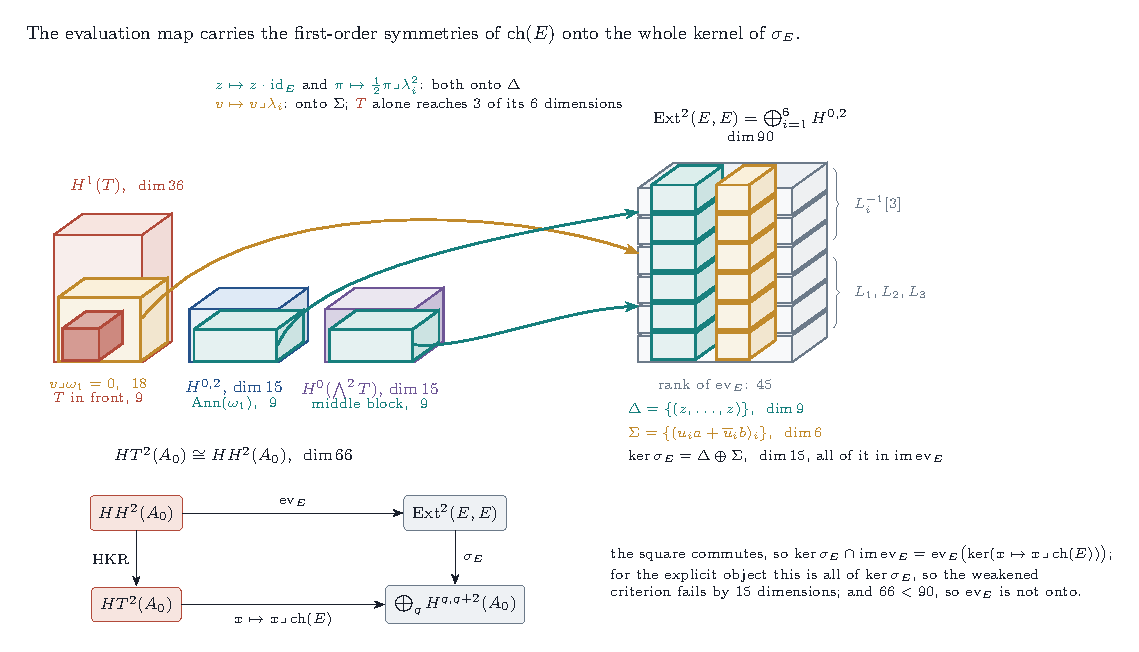
\includegraphics[width=\textwidth]{fig_evaluation}
\caption{\Cref{prop:evaluation} for the explicit object at $n=3$. Left: the
three summands of $HT^{2}(A_{0})$, drawn with heights proportional to their
dimensions, and inside each the part that preserves $\ch(E)$ to first order:
the annihilator of $\omega_{1}$, the deformations killing $\omega_{1}$ with
the polarised $K$-commuting tangent space $T$ in front, and the middle block
of bivectors. Right: $\Ext^{2}(E,E)$ as six stacked copies of $H^{0,2}$, one
per summand of $E$, and inside it the kernel of $\sigma_{E}$: the column
$\Delta$, one and the same class in every layer, and the column $\Sigma$,
whose entries depend on the summand through $u_{i}$. The three arrows are the
evaluation map on the three kernels; the two teal ones both land on
$\Delta$, the ochre one on $\Sigma$, and together they cover the kernel.
Below, the commutative square that makes this a statement about the weakened
criterion of \cite[Question 11.4]{Mar25b}.}
\label{fig:evaluation}
\end{figure}

\begin{remark}[Question 11.4 for split objects]
\label{rem:question114}
For a split object the two criteria stand or fall together, and for the
explicit object both fall completely. \cite[Theorem~9.19]{paperI} makes the first
$n^{2}$ dimensions of the failure uniform over every concentrated object in
every dimension; \Cref{prop:evaluation}(iv) accounts for the remaining
$n(n-1)$ at $n=3$ by the deformations of the two halves $V_{\pm}$ of the
Hodge structure separately, and the equality $\ker\sigma_{E}=\Delta\oplus\Sigma$
says that the two mechanisms exhaust the kernel: nothing in it is
accidental. None of this touches the case for which the question was asked.
A sheaf of positive rank has $z\cdot\ch(E)\ne0$ for every $z\ne0$, so its
$\Delta$ is zero, and whether $\operatorname{ev}_{E}$ kills the deformations
that preserve $\kappa(E)$ is a statement about the sheaf and not about its
Chern character. Markman's candidate in \cite[Section 12]{Mar25b}, a rank
one complex on a principally polarised abelian fourfold with Chern character
on the secant $\langle e^{\pm\sqrt{-d}\Theta}\rangle$, is exactly such a
sheaf, and he records that the verification remains to be done.
\Cref{thm:factor} reduces that verification to one identity on the fourfold,
and \Cref{thm:candidatefails} shows that the identity fails: the candidate
does not satisfy the weakened criterion either.
\end{remark}

\subsubsection*{Solutions of nonzero rank}

We return to the Diophantine problem of \Cref{setup:pte}. By
\Cref{cor:nplusone} a solution with $\ch_{0}(E)\ne0$ needs at least $n+1$
distinct norms, and multiplicity one bounds each level sum by the number of
elements of $\cO_{K}$ of that norm.

\begin{proposition}[The level sums]\label{thm:pterange}
Keep \Cref{setup:pte} and suppose $E$ satisfies \eqref{eq:pteconditions} with
$\ch_{0}(E)\ne0$, so that the $u_{i}$ take $\nu\ge n+1$ distinct norms by
\Cref{cor:nplusone}. Write $N_{1}<\dots<N_{\nu}$ for those norms, $M_{j}$ for
the sum of the $m_{i}$ at level $N_{j}$, and
$r_{K}(N)=\#\{u\in\cO_{K}:\Nm_{K/\QQ}(u)=N\}$. If $\nu=n+1$ then, with
$P=\prod_{k}N_{k}$, $S=\ch_{0}(E)$ and
$D_{j}=N_{j}\prod_{k\ne j}(N_{j}-N_{k})$,
\begin{equation}\label{eq:levelsums}
  M_{j}=(-1)^{n}\,\frac{S\,P}{D_{j}},
\end{equation}
the least $S>0$ making every $M_{j}$ an integer is
$S_{\min}=\operatorname{lcm}_{j}\bigl(|D_{j}|/\gcd(|D_{j}|,P)\bigr)$, and
multiplicity one, \Cref{lem:splitsemireg}(i), forces
$|M_{j}|\le r_{K}(N_{j})$ for every $j$.
\end{proposition}

\begin{proof}
The conditions $T_{r,r}=0$ for $r=1,\dots,n$ say that the linear
functional $f\mapsto\sum_{j}M_{j}f(N_{j})$ kills $x,x^{2},\dots,x^{n}$, hence
sends every polynomial $f$ of degree at most $n$ to $S\,f(0)$. Applying it to
$f(x)=\prod_{k\ne j}(x-N_{k})$, which has degree $n$, gives
\[
  M_{j}\prod_{k\ne j}(N_{j}-N_{k})=S\,(-1)^{n}\prod_{k\ne j}N_{k},
\]
and multiplying by $N_{j}$ turns this into \eqref{eq:levelsums}. The value of
$S_{\min}$ is the definition of a least common multiple, and the bound on
$|M_{j}|$ holds because each $u$ of norm $N_{j}$ contributes at most one term
$m_{i}=\pm1$ to $M_{j}$.
\end{proof}

So the level sums are determined by the norms up to the scale $S$, and they
compete with the supply $r_{K}(N_{j})$ of elements at each level. That
competition is arithmetic. A second mechanism, in the cohomology of $A$,
closes the split route for every $n$ and every set of norms at once.

\begin{corollary}[Sums of line bundles fail both criteria]\label{cor:noline}
Let $A$ be of $(K,-1,n)$-Weil type with $n\ge2$, and let
$E=\bigoplus_{i}L_{i}[p_{i}]^{\oplus m_{i}}$ be a sum of shifted line bundles,
twisted by a common class or not, whose (twisted) Chern character remains of
Hodge type to first order along $\cD_{n,n}$ and has a nonzero Weil component.
Then $\sigma_{E}$ is not injective on the image of $\operatorname{ev}_{E}$:
$E$ is neither semiregular nor semiregular in the weakened sense of
\cite[Question 11.4]{Mar25b}, and it is obstructed to first order along some
direction of the Weil family. In particular every object of \Cref{setup:pte}
satisfying \eqref{eq:pteconditions}, for every $n\ge2$, every field $K$,
every rank and every set of norms, fails both criteria.
\end{corollary}

\begin{proof}
Write $\lambda_{i}$ for the twisted first Chern classes of the summands. If
every $\lambda_{i}$ were a real multiple of $\eta$, it would be a rational
multiple, both classes being rational, and the twisted Chern character
$\sum_{i}m_{i}e^{\lambda_{i}}$ would be a polynomial in $\eta$; its component
in degree $2n$ would then lie in $\QQ\eta^{n}$, which meets the Weil line in
zero by \cite[Proposition~5.1]{paperI}, against the hypothesis. So some $\lambda_{i}$ is
not a real multiple of $\eta$, and \cite[Theorem~9.20]{paperI} applies to the
summand $L_{i}[p_{i}]$. For an object of \Cref{setup:pte} the classes are
$\lambda_{i}=\theta(u_{i})\in R_{0}$, and $R_{0}\cap\QQ\eta=0$; no twist is
needed because $c_{1}(E)=\theta(T_{1,0})=0$ by \eqref{eq:pteconditions}, as
$(1,0)$ is not an excluded pair for $n\ge2$; and \eqref{eq:pteconditions}
gives a flat Chern character with a nonzero Weil component by
\Cref{prop:chintermsofu}.
\end{proof}

\begin{remark}[What the corollary asks of an object]\label{rem:nolinemeaning}
By \Cref{cor:noline} there is no sum of line bundles, at any member of any
Weil family in any dimension, that could run the semiregularity argument in
either form. The reason is \cite[Proposition~9.15(i)]{paperI}: the
only divisor class that stays of type $(1,1)$ across the whole family is the
polarisation, so every line bundle summand off that line is obstructed in
some direction of the family, and the semiregularity map, whose composite
with the obstruction is contraction with the flat class $\ch(E)$, cannot see
it. The object the argument needs is one with no rank one
summand off the polarisation line, of positive rank, indecomposable enough
that its Atiyah class contracted with every direction of $T$ vanishes.
Markman's reflexive sheaves at $n=3$ are of that kind, and nothing here
says that their analogues at $n\ge4$ do not exist.
\end{remark}

\subsection{Convolutions of line bundles}\label{ssec:convolutions}

After \Cref{cor:noline} the next objects built from line bundles are their
convolutions, the iterated cones of shifted line bundles. Their Chern
character is the same signed sum of exponentials as for a direct sum, but
their $\Ext$ groups are cut down by the maps between the pieces, so the
argument of \cite[Theorem~9.20]{paperI} no longer applies as it stands. This
subsection shows that fewer than $2n$ pieces with nondegenerate differences
never serve (\Cref{thm:fewpieces}); writes down, at a CM member for
$K=\QQ(i)$, a signed sum of $2\cdot4^{n-1}$ line bundles that is exactly a
real Weil class (\Cref{prop:weilpieces}); and determines, for the
convolutions of those pieces with three multiples of the polarisation at
$n=3$, which products in the twisted differential can act on the $525$
diagonal classes of degree two, of which at least $468$ must disappear
before the polarised criterion can hold (\Cref{thm:esixdiagonal}). Nothing
enters the diagonal, cup products remove at most $276$ of these classes, and
everything else would have to be removed by fourfold products along a path
through the three multiples and one of the Weil pieces: one family of them
for some placements of the multiples, and two families that exclude each
other for the others (\Cref{prop:mixedplacement}); one order of the pieces
gives a convolution that solves the Maurer--Cartan equation
(\Cref{prop:explicitconvolution}). Off the diagonal, the classes between two
pieces that differ in every coordinate are reached by no product
(\Cref{lem:allthree}), and no
convolution of these pieces meets the polarised criterion
(\Cref{thm:noconvolution}). At $n=4$ the same classes, now between pieces
that differ in three coordinates, are reached by no product in any
convolution, and they exclude every convolution whose $128$ pieces
$L_{\zeta}$ occupy two shifts (\Cref{thm:efourtwolevels}) or three
consecutive ones (\Cref{thm:efourthreelevels}); with the groups between
pieces whose shifts differ by two or three (\Cref{lem:efourspread}) they
exclude every convolution whose pieces have their shifts within five
consecutive values (\Cref{cor:efourfive}); the diagonal classes at a lonely
shift (\Cref{lem:efourlonely}) and the interleaved shifts
(\Cref{prop:efourpairs}) extend this to six (\Cref{cor:efoursix}).

\begin{setupenv}[Convolutions]\label{setup:convolution}
Let $A$ be an abelian variety of dimension $g$ with a flat K\"ahler metric,
and let $L_{1},\dots,L_{m}$ be line bundles on $A$ with hermitian metrics of
constant curvature, hermitian forms $H_{1},\dots,H_{m}$ and pairwise distinct
first Chern classes. For integers $d_{1},\dots,d_{m}$ put
$P_{a}=L_{a}[-d_{a}]$. A \emph{convolution} of $P_{1},\dots,P_{m}$ is an
object $E$ given by a one-sided twisted
complex\footnote{Every object obtained from $P_{1},\dots,P_{m}$ by iterated
cones in this order is of this form, because the Dolbeault complexes form a
differential graded enhancement of the full subcategory of line bundles. All
the objects of this subsection are given in this way.}
\[
  \Bigl(\,\bigoplus_{a}\cA^{0,*}(L_{a})[-d_{a}],\ \bar\partial+\delta\Bigr),
  \qquad
  \delta=(\delta_{ab})_{a<b},\quad
  \delta_{ab}\in\cA^{0,1+d_{a}-d_{b}}\bigl(L_{a}^{-1}\otimes L_{b}\bigr),
\]
with $\bar\partial\delta+\delta\circ\delta=0$, so that
$\ch(E)=\sum_{a}(-1)^{d_{a}}e^{c_{1}(L_{a})}$. Write
$\cA(a,b)=\cA^{0,*}(L_{a}^{-1}\otimes L_{b})$ and $\cH(a,b)$ for its harmonic
forms, so that $\cH^{q}(a,b)\cong H^{q}(A,L_{a}^{-1}\otimes L_{b})$, and write
$\pi$, $G$ and $h=\bar\partial^{*}G$ for the harmonic projection, the Green
operator and the homotopy, with $1-\pi=\bar\partial h+h\bar\partial$ and
$\pi h=h\pi=h^{2}=0$. A form of degree $q$ in $\cA(a,b)$ is a morphism
$P_{a}\to P_{b}$ of degree $w=q-d_{a}+d_{b}$; we call $q$ its $\Ext$ degree
and, when $w=1$, call $q-1$ its \emph{excess}. When $H_{b}-H_{a}$ is
nondegenerate, $\cH(a,b)$ is concentrated in the single degree
$n(H_{b}-H_{a})$, the number of negative eigenvalues \cite[Chapter~3]{BL04}.
\end{setupenv}

\begin{lemma}[The harmonic model]\label{lem:harmonicmodel}
In \Cref{setup:convolution}:
\begin{enumerate}[label=\textup{(\roman*)},leftmargin=2.6em,itemsep=2pt]
\item $E$ is isomorphic to a convolution of the same pieces with
  $h\delta=0$, and then $\delta=\delta^{H}-h(\delta\circ\delta)$ with
  $\delta^{H}=\pi\delta$ harmonic. Substituting repeatedly, every
  $\delta_{ab}$ is a finite sum of planar binary trees whose leaves are
  components $\delta^{H}_{cd}$ with $c<d$, whose internal vertices compose,
  and whose internal edges carry $-h$.
\item $\Ext^{*}(E,E)$ is the cohomology of
  $\cH_{E}=\bigoplus_{a,b}\cH(a,b)$, graded by $w$, with the differential
  $d_{E}=\sum_{k\ge0}\pi\,Q(-hQ)^{k}$, where $Q=[\delta,-]$.
\item For $x\in\cH(a,b)$, the component of $d_{E}(x)$ in $\cH(c,e)$ is a sum
  of terms $\pm\pi\,T$, one for each planar binary tree $T$ with $k\ge2$
  leaves, internal vertices composing, $-h$ on the internal edges other
  than the root, whose leaves read in order are the components along a path
  $c=a_{0}\to a_{1}\to\dots\to a_{k}=e$ in which one step is
  $x\colon a\to b$ and the others are components $\delta^{H}_{a_{j}a_{j+1}}$
  with $a_{j}<a_{j+1}$. The $\Ext$ degree of such a term is the sum of the
  $\Ext$ degrees of its leaves minus $k-2$.
\end{enumerate}
\end{lemma}

The terms with $k$ leaves in (iii) are the Massey products of length $k$ of
the pieces;\footnote{In the language of $A_{\infty}$-categories they are the
higher products $m_{k}$ of the minimal model of the line bundles, evaluated
on the Maurer--Cartan element $\delta^{H}$ of the twisted complex; for
$k=2$ they are cup products.} (iii) is all that is used of them below.

\begin{proof}
(i) Suppose $h\delta_{cd}=0$ for $d-c<r$. Conjugating by $1+g$, with $g$ of
degree $0$ supported at distance $r$, replaces $\delta_{ab}$ for $b-a=r$ by
$X_{ab}+\bar\partial g_{ab}$, where $X_{ab}$ depends only on $\delta$, and
leaves the components at smaller distance unchanged. With
$g_{ab}=-hX_{ab}$ the new component is $X_{ab}-\bar\partial hX_{ab}$, and
$h\bar\partial h=h(1-\pi-h\bar\partial)=h$ gives $h(X_{ab}-\bar\partial
hX_{ab})=0$. Induction on $r$ gives $h\delta=0$, and then
$\delta=\pi\delta+\bar\partial h\delta+h\bar\partial\delta
=\delta^{H}-h(\delta\circ\delta)$ by the Maurer--Cartan equation. The
component $(\delta\circ\delta)_{ab}$ involves only components at distance
less than $b-a$, so the substitution ends.
(ii) The endomorphism complex of $E$ is $\bigoplus_{a,b}\cA(a,b)$ with the
differential $\bar\partial+Q$. Blockwise, the inclusion of harmonic forms,
$\pi$ and $-h$ form a strong deformation retraction of
$(\bigoplus\cA(a,b),\bar\partial)$ onto $(\cH_{E},0)$, and $Q$ raises $b-a$,
so $hQ$ is nilpotent. The basic perturbation lemma gives a homotopy
equivalence of $(\bigoplus\cA(a,b),\bar\partial+Q)$ with $(\cH_{E},d_{E})$,
with the chain maps $\iota_{E}=\sum_{k}(-hQ)^{k}$ on $\cH_{E}$ and
$\pi_{E}=\pi\sum_{k}(-Qh)^{k}$. (iii) Each $Q$ in $d_{E}$ composes with one
component of $\delta$ on the left or on the right; writing that component as
in (i) gives the trees, the edges from (i) and those from $d_{E}$ being
exactly the internal edges other than the root. Composition adds degrees,
$h$ lowers them by one, and a binary tree with $k$ leaves has $k-2$ internal
edges.
\end{proof}

\begin{lemma}[The index of a sum]\label{lem:indexsum}
For hermitian forms $X,Y$ on $\CC^{g}$, $n(X+Y)\le n(X)+n(Y)$. If
$H_{1}+\dots+H_{k}=0$, then $\sum_{j}n(H_{j})\ge g-\dim\ker H_{i}$ for every
$i$; in particular $\sum_{j}n(H_{j})\ge g$ when one $H_{i}$ is
nondegenerate.
\end{lemma}

\begin{proof}
A subspace on which $X+Y$ is negative definite meets the subspaces on which
$X\ge0$ and $Y\ge0$, of codimensions $n(X)$ and $n(Y)$, only in zero, so its
dimension is at most $n(X)+n(Y)$. For the second statement,
$-H_{i}=\sum_{j\ne i}H_{j}$ gives
$g-n(H_{i})-\dim\ker H_{i}=n(-H_{i})\le\sum_{j\ne i}n(H_{j})$.
\end{proof}

\begin{theorem}[Fewer than $2n$ pieces]\label{thm:fewpieces}
Let $A$ be of $(K,-1,n)$-Weil type with $n\ge2$, and let $E$ be a
convolution of $m<2n$ shifted line bundles whose differences $H_{b}-H_{a}$
are all nondegenerate. Suppose that $\ch(E)$ remains of Hodge type to first
order along $\cD_{n,n}$ and has a nonzero Weil component, as every polarised
character $N\omega_{1}+p(\theta)$ with $N\ne0$ does. Then there is
$v\in T_{[A]}\cD_{n,n}$ with
\[
  \operatorname{ev}_{E}(v)\ne0
  \qquad\text{and}\qquad
  \sigma_{E}\bigl(\operatorname{ev}_{E}(v)\bigr)=0 ,
\]
so $\sigma_{E}$ is not injective, and for a polarised character
$\dim\Ext^{2}(E,E)>r(\ch E)$ by \Cref{thm:p2primenumber}(iv).
\end{theorem}

\begin{proof}
First, no element of degree one of $\cH_{E}$ has a differential with a
nonzero component in the diagonal classes $\cH^{2}(c,c)=H^{2}(A,\cO_{A})$.
Such a component is a sum of terms of \Cref{lem:harmonicmodel}(iii) whose
$k$ leaves have degree one and run around a closed path $c\to\dots\to c$; the
pieces before the step $x$ increase from $c$ and those after it increase to
$c$, so the path passes through $k$ distinct pieces and $k\le m$. Its
leaves have $\Ext$ degrees $q_{j}=n(H_{a_{j+1}}-H_{a_{j}})$, and the output
has $\Ext$ degree $\sum_{j}q_{j}-(k-2)=2$, so $\sum_{j}q_{j}=k<2n$. The $k$
differences are nondegenerate and add up to zero, so \Cref{lem:indexsum}
gives $\sum_{j}q_{j}\ge g=2n$, a contradiction. Hence taking diagonal
components gives a well defined map
$\pi_{D}\colon\Ext^{2}(E,E)\to\bigoplus_{a}H^{2}(A,\cO_{A})$.

Next, $\operatorname{ev}_{E}(v)=v\lrcorner\mathrm{At}(E)$, as in the proof
of \cite[Theorem~9.20]{paperI}. In the twisted complex the Atiyah class is
represented by the commutator of the Chern $(1,0)$-connection
$\bigoplus_{a}\nabla_{a}$ with $\bar\partial+\delta$; its diagonal entries
are the curvatures $F_{a}$, constant forms representing $c_{1}(L_{a})$, and
its other entries $\nabla\delta_{ab}$ lie above the diagonal. So
$\operatorname{ev}_{E}(v)$ is represented by an upper triangular $z$ with
$z_{aa}=v\lrcorner F_{a}$, and in $\cH_{E}$ by $\pi_{E}(z)$. The operators
$Q$ and $h$ preserve upper triangular forms and $Q$ makes them strictly upper
triangular, so the diagonal of $\pi_{E}(z)$ is that of $\pi(z)$, and
$\pi_{D}(\operatorname{ev}_{E}(v))=(v\lrcorner c_{1}(L_{a}))_{a}$.

If every $c_{1}(L_{a})$ were a real multiple of the polarisation, it would
be a rational one and $\ch(E)$ a polynomial in it, whose component in degree
$2n$ meets the Weil line in zero by \cite[Proposition~5.1]{paperI}. So some
$c_{1}(L_{a})$ is not, and by \cite[Proposition~9.15(i)]{paperI} some
$v\in T_{[A]}\cD_{n,n}$ has $v\lrcorner c_{1}(L_{a})\ne0$; then
$\pi_{D}(\operatorname{ev}_{E}(v))\ne0$, while
$\sigma_{E}(\operatorname{ev}_{E}(v))=v\lrcorner\ch(E)=0$.
\end{proof}

\cite[Theorem~9.20]{paperI} is the case $\delta=0$, with any number of pieces. A
convolution reaches its diagonal classes once it has $2n$ pieces, when a
cycle through all of them can have total index $2n$, the equality case of
\Cref{lem:indexsum}. A convolution meeting the polarised criterion must
therefore have at least $2n$ pieces, or pieces with degenerate differences.
The next construction has both.

\begin{proposition}[A pure Weil class from line bundles]
\label{prop:weilpieces}
Let $E_{0}=\CC/\ZZ[i]$, $A=E_{0}^{2n}$ with coordinates $z_{1},\dots,z_{2n}$
and $n\ge2$, let $K=\QQ(i)$ act by $i$ on $z_{1},\dots,z_{n}$ and by $-i$
on $z_{n+1},\dots,z_{2n}$, and let $\theta$ be the product principal
polarisation; then $A$ is of $(\QQ(i),-1,n)$-Weil type, a CM member as in
\cite[Remark~17.6]{paperI}. Write $B_{j}$ for the surface with coordinates
$(z_{j},z_{n+j})$, so that $A=B_{1}\times\dots\times B_{n}$. For $p\in\ZZ$
and $\zeta\in\mu_{4}^{n}$ let $L_{\zeta}$ be a line bundle whose hermitian
form is $\bigl(\begin{smallmatrix}p&\zeta_{j}\\ \bbar\zeta_{j}&p
\end{smallmatrix}\bigr)$ on $B_{j}$ and zero between different surfaces, and
put $\alpha=\prod_{j}\tfrac{i}{2}\,dz_{j}\wedge d\bar z_{n+j}$.
\begin{enumerate}[label=\textup{(\roman*)},leftmargin=2.6em,itemsep=2pt]
\item $\alpha$ and $\bbar\alpha$ span the Weil classes of $A$, and
  \[
    \sum_{\prod\zeta=1}e^{c_{1}(L_{\zeta})}
    -\sum_{\prod\zeta=-1}e^{c_{1}(L_{\zeta})}
    =2\cdot4^{n-1}\,(\alpha+\bbar\alpha).
  \]
\item For distinct integers $t_{1},t_{2},t_{3}$ and signs $\sigma_{i}$, the
  character
  $\gamma=2\cdot4^{n-1}(\alpha+\bbar\alpha)+\sum_{i}\sigma_{i}e^{t_{i}\theta}$
  has Hankel rank $3$, so $r(\gamma)=7n^{2}-2n$. A convolution with this
  character of the $2\cdot4^{n-1}$ bundles $L_{\zeta}$, with
  $(-1)^{d}=\prod\zeta$, and of three line bundles $M_{i}$ with
  $c_{1}(M_{i})=t_{i}\theta$ has $2\cdot4^{n-1}+3$ pieces and
  $(2\cdot4^{n-1}+3)\,n(2n-1)$ diagonal classes of degree two: $525$
  against $r=57$ at $n=3$, and $3668$ against $104$ at
  $n=4$.\footnote{At $n=2$ the same construction has $8+3=11$ pieces and
  $66$ diagonal classes against $r=24$.}
\end{enumerate}
\end{proposition}

\begin{proof}
The hermitian forms have imaginary parts integral on $\ZZ[i]^{2n}$, so the
line bundles exist. On $B_{j}$ write $c_{1}$ of the restriction as
$p(a_{j}+b_{j})+\zeta_{j}c_{j}+\bbar\zeta_{j}c'_{j}$, where
$a_{j}=\tfrac i2dz_{j}\wedge d\bar z_{j}$,
$b_{j}=\tfrac i2dz_{n+j}\wedge d\bar z_{n+j}$,
$c_{j}=\tfrac i2dz_{j}\wedge d\bar z_{n+j}$ and
$c'_{j}=\tfrac i2dz_{n+j}\wedge d\bar z_{j}$. Since $c_{j}^{2}=c_{j}'^{2}=0$,
\[
  e^{c_{1}(L_{\zeta})}=\prod_{j}f_{j}(\zeta_{j}),\qquad
  f_{j}(z)=e^{p(a_{j}+b_{j})}\bigl(1+zc_{j}+\bbar zc'_{j}+c_{j}c'_{j}\bigr).
\]
For
$u\in\mu_{4}$, $\tfrac12(u+\bbar u)$ is $u$ when $u=\pm1$ and $0$ when
$u=\pm i$, so the left side of (i) is
$\tfrac12\bigl(\prod_{j}\sum_{z}zf_{j}(z)+\prod_{j}\sum_{z}\bbar zf_{j}(z)\bigr)$.
Now $\sum_{z\in\mu_{4}}z=\sum z^{2}=0$ and $\sum|z|^{2}=4$, so
$\sum_{z}zf_{j}(z)=4e^{p(a_{j}+b_{j})}c'_{j}=4c'_{j}$, because $a_{j}c'_{j}$
and $b_{j}c'_{j}$ repeat a differential, and likewise
$\sum_{z}\bbar zf_{j}(z)=4c_{j}$. This gives
$2\cdot4^{n-1}(\prod c'_{j}+\prod c_{j})=2\cdot4^{n-1}(\bbar\alpha+\alpha)$.
The differentials $dz_{j}$, $j\le n$, and $d\bar z_{n+j}$ span the
$i$-eigenspace of $K$ on $H^{1}(A,\CC)$, and $\alpha$ spans its top exterior
power, which is a Weil class, and $\bbar\alpha$ the conjugate one. (ii) The
moments $\mu_{m}=\sum_{i}\sigma_{i}t_{i}^{m}$ make the Hankel matrix of
\Cref{setup:p2prime} a product of Vandermonde matrices of rank $3$, and
\Cref{thm:p2primenumber}(ii) gives $r$. The counts are immediate.
\end{proof}

The pieces $L_{\zeta}$ and $L_{\zeta'}$ have a degenerate difference as soon
as $\zeta$ and $\zeta'$ share a coordinate, so \Cref{thm:fewpieces} does not
apply to them, and there are more than $2n$ of them. The rest of this
subsection computes what the Massey products can do to the diagonal classes
of such a convolution. The pieces are external products over the surfaces
$B_{j}$, and the first tool is a bound on how far a product can lower the
degree on each surface.

\begin{lemma}[Degree drop on a product]\label{lem:degreedrop}
Let $A=B_{1}\times\dots\times B_{n}$ with a product metric, and let every
$L_{a}$ be an external product with a product metric. Decompose the leaves
of a term of \Cref{lem:harmonicmodel}(iii) with $k$ leaves into tensor
products of harmonic forms on the factors. Then the output has degree
$s_{j}-d_{j}$ on $B_{j}$, where $s_{j}$ is the sum of the degrees of the
leaves on $B_{j}$ and $d_{j}\ge0$, $\sum_{j}d_{j}=k-2$, and
\[
  d_{j}\le\max(0,\,u_{j}-2),
\]
where $u_{j}$ is the number of leaves whose component on $B_{j}$ is not a
multiple of the unit section of $\cO_{B_{j}}$ (such a unit occurs only where
source and target agree on $B_{j}$).
\end{lemma}

\begin{proof}
The Laplacian is $\Delta=\sum_{j}\Delta_{j}$, so $h=\sum_{j}h_{j}$ with
$h_{j}=\bar\partial_{j}^{*}G=G\bar\partial_{j}^{*}$, which lowers the degree
on $B_{j}$ by one and keeps the others; expand every internal edge
accordingly, and let $d_{j}$ be the number of edges carrying $h_{j}$. Let
$V_{j}$, $U_{j}$ and $W_{j}$ be the forms whose component on $B_{j}$ is
$\Delta_{j}$-harmonic, a multiple of the unit, or in the image of
$\bar\partial_{j}^{*}$. The operators $G$ and $h_{i}$, $i\ne j$, preserve all
three, $h_{j}$ kills $V_{j}$ and $W_{j}$, $\pi$ kills $W_{j}$, and
multiplication by an element of $U_{j}$ preserves $V_{j}$, $U_{j}$ and
$W_{j}$. For an edge $e$ carrying $h_{j}$ let $N(e)$ be the set of leaves
below $e$ whose component on $B_{j}$ is not a unit. If $|N(e)|\le1$ the
value below $e$ lies in $V_{j}$ and the term vanishes. If $e$ lies below the
next such edge $e'$ with $N(e)=N(e')$, everything composed in between lies
in $U_{j}$, the value at $e'$ lies in $W_{j}$, and the term vanishes; if
$N(e)$ is the set of all $u_{j}$ such leaves for the highest such edge, the
value at the root lies in $W_{j}$ and $\pi$ kills it. So in a nonzero term
the sets $N(e)$ are distinct, of size at least two, different from the whole
set, and pairwise nested or disjoint. Together with the whole set they form
a family of that kind, which has at most $u_{j}-1$ members, since its members
are the internal vertices of a forest with $u_{j}$ leaves in which every
internal vertex has at least two children. Hence $d_{j}\le u_{j}-2$.
\end{proof}

\begin{proposition}[Nothing enters the diagonal]\label{prop:nothingenters}
Keep \Cref{prop:weilpieces} with $n\ge3$, and let $t_{1},t_{2},t_{3}$ be
distinct with $|t_{i}-p|\ge2$. For every convolution $E$ of the pieces
$L_{\zeta}$ and $M_{i}$, in any order, with any shifts of the given parities
and with the pieces twisted by any line bundles of degree zero, no element of
degree one of $\cH_{E}$ has a differential with a nonzero diagonal
component. Consequently
\[
  \dim\Ext^{2}(E,E)\;\ge\;\dim\ker\bigl(d_{E}|_{D^{2}}\bigr),
  \qquad
  D^{2}=\bigoplus_{a}H^{2}(A,\cO_{A}).
\]
\end{proposition}

\begin{proof}
As in the proof of \Cref{thm:fewpieces}, a term that reaches the diagonal
runs around a closed path of distinct pieces whose $k$ steps have degree one
and total excess $0$. The step from $L_{\zeta}$ to $L_{\zeta'}$ has $\Ext$
degree $1$ on each surface where $\zeta_{j}\ne\zeta'_{j}$, the difference
there having eigenvalues $\pm|\zeta'_{j}-\zeta_{j}|$, and at least $0$
elsewhere. If $\prod\zeta=\prod\zeta'$ the two differ on at least two
surfaces; otherwise the step has even $\Ext$ degree, the shifts having
opposite parities. Either way its excess is at least $1$. The difference
between $L_{\zeta}$ and $M_{i}$ has eigenvalues $t_{i}-p\pm1$ on every
surface, so it is definite: the step has $\Ext$ degree $0$ and excess $-1$
if it goes up the value $\phi$, where $\phi(L_{\zeta})=p$ and
$\phi(M_{i})=t_{i}$, and $\Ext$ degree $2n$ and excess $2n-1$ if it goes
down; the same holds between the $M_{i}$. A maximal run of the cycle through
the $M_{i}$ starts and ends at the value $p$, or is the whole cycle, so it
has at least one step down and at most three steps up; its excess is at least
$2n-1-3\ge2$. So every cycle has excess at least $1$. Twisting by line
bundles of degree zero leaves the forms unchanged and can only make some
$\cH(a,b)$ vanish. For the inequality, the diagonal components of cocycles
of degree two vanish on coboundaries, so $\dim\Ext^{2}(E,E)$ is at least the
dimension of their image, which contains the kernel of $d_{E}$ on $D^{2}$.
\end{proof}

At $n=2$ the bound on a run is $0$ and a cycle through the three multiples
can reach the diagonal; this is why the analysis below starts at $n=3$.

\begin{figure}[tbp]
\centering
  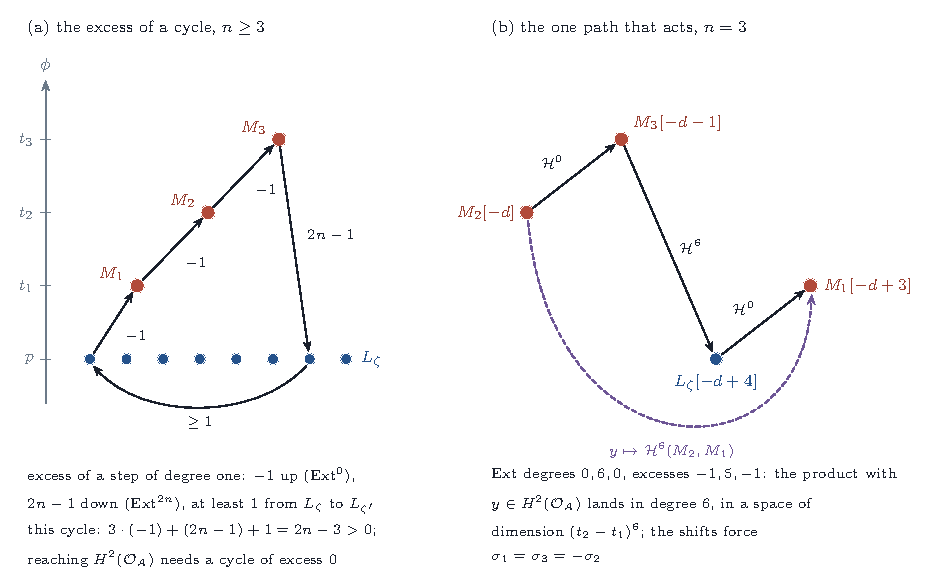
\includegraphics[width=\textwidth]{fig_convolutions}
\caption{The pieces of \Cref{prop:weilpieces} at their values $\phi$, with
$\phi(L_{\zeta})=p$ and $\phi(M_{i})=t_{i}$. (a) A step of degree one
between pieces with a definite difference has $\Ext$ degree $0$ going up
and $2n$ going down, so excess $-1$ or $2n-1$; a step between two
$L_{\zeta}$ has excess at least $1$. The cycle drawn runs up through all
three $M_{i}$ and down once, the worst case, and still has excess
$2n-3>0$, so for $n\ge3$ no term reaches the diagonal
(\Cref{prop:nothingenters}). (b) The one path whose products act on the
diagonal at $n=3$ when the $t_{i}$ lie above $p$
(\Cref{thm:esixdiagonal}(i)), drawn at the same heights
and in the order of the convolution, with the $\Ext$ degrees of its steps
and the shifts they force; the dashed arrow is the value of the product with
a diagonal class $y$.}
\label{fig:convolutions}
\end{figure}

\begin{proposition}[Cup products on the diagonal]\label{prop:cupkernel}
Keep \Cref{prop:nothingenters} with $n=3$, so that $D^{2}$ has dimension
$35\cdot15=525$. The terms of $d_{E}$ on $D^{2}$ with two leaves, the cup
products, vanish on the $45$ diagonal classes of the $M_{i}$, and on the
$480$ diagonal classes of the $L_{\zeta}$ they have a kernel of dimension at
least $204$. So their kernel on $D^{2}$ has dimension at least $249$.
\end{proposition}

\begin{proof}
For $y=(y_{a})\in D^{2}$ the cup products in $\cH(a,b)$ are
$(y_{a}-y_{b})\wedge\delta^{H}_{ab}$, since $y$ has even degree. On a surface
where the pieces differ, $\delta^{H}_{ab}$ has degree $1$, the only degree of
the cohomology there, and the product with a component of $y$ of positive
degree lands in a degree where the cohomology vanishes. The pieces $M_{i}$
differ from every other piece on every surface, which gives the first
statement. Write $y_{a}$ by its type $\tau\in\{0,1,2\}^{3}$, $|\tau|=2$, the
degrees on the three surfaces: three types $(2,0,0)$ of dimension one and
three types $(1,1,0)$ of dimension four. The degree count on each surface
and the parity of $\Ext$ degrees show that $L_{\zeta}$ and $L_{\zeta'}$ can
carry a nonzero cup product on the type $\tau$ only if either $\zeta'$
differs from $\zeta$ by a sign in one coordinate outside the support of
$\tau$, or $\zeta'$ is $\zeta$ multiplied by $(i,i)$ or $(-i,-i)$ in two
coordinates and $\tau$ is $2$ on the third. Let $\Gamma_{\tau}$ be the graph
on the $32$ pieces with these edges. If each component $y^{\tau}$ is
constant on the connected components of $\Gamma_{\tau}$, every cup product
vanishes. For $\tau=(2,0,0)$ the coordinate $\zeta_{1}$ is constant along
the edges, and the eight pieces with a given $\zeta_{1}$ are connected, so
$\Gamma_{\tau}$ has $4$ components; for $\tau=(1,1,0)$ the edges change the
sign of $\zeta_{3}$ only, and $\Gamma_{\tau}$ has $16$ components. The
kernel therefore contains a space of dimension $3\cdot4\cdot1+3\cdot16\cdot4
=12+192=204$.
\end{proof}

\begin{theorem}[The diagonal on $E_{0}^{6}$]\label{thm:esixdiagonal}
Let $n=3$ and let $E$ be a convolution of the $32$ bundles $L_{\zeta}$ and
of $M_{1},M_{2},M_{3}$ as in \Cref{prop:weilpieces}, with
$p+2\le t_{1}<t_{2}<t_{3}$ and signs $\sigma_{i}$, so that
$\ch(E)=32(\alpha+\bbar\alpha)+\sum_{i}\sigma_{i}e^{t_{i}\theta}$ and the
polarised criterion asks for $\dim\Ext^{2}(E,E)=57$.
\begin{enumerate}[label=\textup{(\roman*)},leftmargin=2.6em,itemsep=2pt]
\item The Massey products of length at least three vanish on $D^{2}$, except
  those of length four along a path
  $M_{2}\to M_{3}\to L_{\zeta}\to M_{1}$ taken in this order in the
  convolution, which occur only if $\sigma_{1}=\sigma_{3}=-\sigma_{2}$ and
  take values in
  $\cH^{6}(M_{2},M_{1})\cong H^{6}\bigl(A,\cO_{A}(-(t_{2}-t_{1})\theta)\bigr)$,
  of dimension $(t_{2}-t_{1})^{6}$.
\item $\dim\Ext^{2}(E,E)\ge249-\min\bigl(249,(t_{2}-t_{1})^{6}\bigr)$, and
  $\dim\Ext^{2}(E,E)\ge249$ unless the order and the signs are as in (i).
  In particular $E$ does not meet the polarised criterion when
  $t_{2}-t_{1}\le2$, since $249-64=185>57$, nor when the signs or the order
  differ from (i).
\item If $E$ meets the polarised criterion, then the length four products
  of (i) have rank at least $249-57=192$ on the kernel of the cup products,
  and $t_{2}-t_{1}\ge3$.
\end{enumerate}
The same holds for $t_{1}<t_{2}<t_{3}\le p-2$ with $E$ replaced by its dual.
\end{theorem}

\begin{proof}
(i) By \Cref{lem:harmonicmodel}(iii) a term with $k\ge3$ leaves acting on
$y\in H^{2}(\cO_{A})$ at a piece $c$ runs along a chain
$s=a_{0}\to\dots\to a_{k-1}=e$ of distinct pieces, increasing in the order
of the convolution, whose $k-1$ steps are components of degree one, with $y$
inserted at $c$. Its value lies in $\cH(s,e)$, in $\Ext$ degree
$2+\sum_{j}q_{j}-(k-2)=3+\varepsilon$, where $\varepsilon$ is the sum of the
excesses of the steps; so $-3\le\varepsilon\le3$, and $\cH(s,e)$ must be
nonzero in degree $3+\varepsilon$. By the proof of \Cref{prop:nothingenters}
a step between two $L_{\zeta}$ has excess at least $1$, with equality only
between pieces of opposite parities, and a step between pieces at different
values of $\phi$ has excess $-1$ and $\Ext$ degree $0$ going up, excess $5$
and $\Ext$ degree $6$ going down. Let $U$ and $D$ be the numbers of steps
up and down and $\lambda$ the total excess of the steps between two
$L_{\zeta}$, so that $\varepsilon=5D-U+\lambda$. For two distinct
$L_{\zeta}$, $L_{\zeta'}$ differing in $m\ge1$ coordinates, $\cH(L_{\zeta},
L_{\zeta'})$ vanishes above degree $6-m$; for pieces at different values it
sits in degree $0$ if the target is higher and in degree $6$ if it is lower.

Two observations remove chains. First, a chain of total excess $-2$ has no
step down, and so consists of steps between $L_{\zeta}$ followed by at most
three steps up. Second, let $a\to b\to c$ be two consecutive steps of
$\Ext$ degree $0$, sections $x_{ab}$ and $x_{bc}$ of line bundles. The
Maurer--Cartan equation $\pi(\delta\circ\delta)=0$ of the proof of
\Cref{prop:explicitconvolution}(i) has, in $\cH^{0}(a,c)$, one term for each
chain from $a$ to $c$ of total excess $-2$. If $a\to b\to c$ is the only such
chain, the equation reads $x_{ab}x_{bc}=0$, a product of holomorphic
sections being holomorphic and so harmonic; since $A$ is connected, $x_{ab}$
or $x_{bc}$ vanishes, and every term along a chain through both steps is
zero.

Here every step up ends at one of $M_{1},M_{2},M_{3}$, so $U\le3$, and
$D\le1$. If $D=0$, the chain is $r\ge0$ pieces $L_{\zeta}$ followed by
multiples in increasing order. When it ends at an $L_{\zeta}$, $k\ge3$ gives
$\lambda\ge2$, so $s$ and $e$ differ in one coordinate and $\lambda=2$; then
the two steps change the parity twice, whereas $s$ and $e$ have opposite
parities. When it ends at a multiple, $e$ lies above $s$, so $\varepsilon=-3$,
which forces $U=3$, $\lambda=0$ and the chain $L_{\zeta}\to M_{1}\to
M_{2}\to M_{3}$; by the first observation $L_{\zeta}\to M_{1}\to M_{2}$ is the
only chain of excess $-2$ from $L_{\zeta}$ to $M_{2}$, and the second removes
it. If $D=1$, then $U\ge2+\lambda$, so $(U,\lambda)$ is $(2,0)$, $(3,0)$ or
$(3,1)$ and $\varepsilon$ is $3$, $2$ or $3$. For $\varepsilon=3$ the piece
$s$ is a multiple and $e$ lies below it. With $(3,1)$ the three steps up
would end at three multiples other than $s$, which do not exist. With $(2,0)$
the chain has three steps, and a step down lands at an $L_{\zeta}$, since a
fourth multiple does not exist. It is $M_{1}\to M_{2}\to M_{3}\to L_{\zeta}$,
removed by the second observation at $M_{1}\to M_{2}\to M_{3}$; or
$M_{a}\to M_{b}\to L_{\zeta}\to M_{c}$ with $t_{a}<t_{b}$ and $t_{c}<t_{a}$,
that is $M_{2}\to M_{3}\to L_{\zeta}\to M_{1}$; or
$M_{a}\to L_{\zeta}\to M_{b}\to M_{c}$ with $t_{b}<t_{c}<t_{a}$, that is
$M_{3}\to L_{\zeta}\to M_{1}\to M_{2}$, removed at $L_{\zeta}\to M_{1}\to
M_{2}$. For $\varepsilon=2$, with $(U,\lambda)=(3,0)$, the pieces $s$ and $e$
are $L_{\zeta}$ differing in one coordinate; the last step is the step down,
preceded by three steps up from $s$, so the chain is $L_{\zeta}\to M_{1}\to
M_{2}\to M_{3}\to L_{\zeta'}$, removed at $L_{\zeta}\to M_{1}\to M_{2}$.

Only $M_{2}\to M_{3}\to L_{\zeta}\to M_{1}$ remains. Its steps have $\Ext$
degrees $0$, $6$ and $0$, so degree one forces $d_{M_{3}}=d_{M_{2}}+1$,
$d_{L}=d_{M_{3}}-5$ and $d_{M_{1}}=d_{L}+1$; this gives the signs, and the
value lies in
$\cH^{3+d_{M_{2}}-d_{M_{1}}}(M_{2},M_{1})=\cH^{6}(M_{2},M_{1})$, whose
dimension is $|\chi(\cO_{A}((t_{1}-t_{2})\theta))|=(t_{2}-t_{1})^{6}$.
(ii) By \Cref{prop:nothingenters} it suffices to bound the kernel of $d_{E}$
on $D^{2}$. By \Cref{prop:cupkernel} the cup products have a kernel $Y$ of
dimension at least $249$, and on $Y$ the differential is the sum of the
products of (i), of rank at most $(t_{2}-t_{1})^{6}$. (iii) follows from
(ii). For the dual, $E\mapsto E^{\vee}$ preserves $\Ext^{2}$ and sends the
configuration with $p$, $t_{i}$ to the one with $-p$, $-t_{i}$, the set of
the $L_{\zeta}$ being stable under $\zeta\mapsto-\zeta$.
\end{proof}

\begin{figure}[tbp]
\centering
  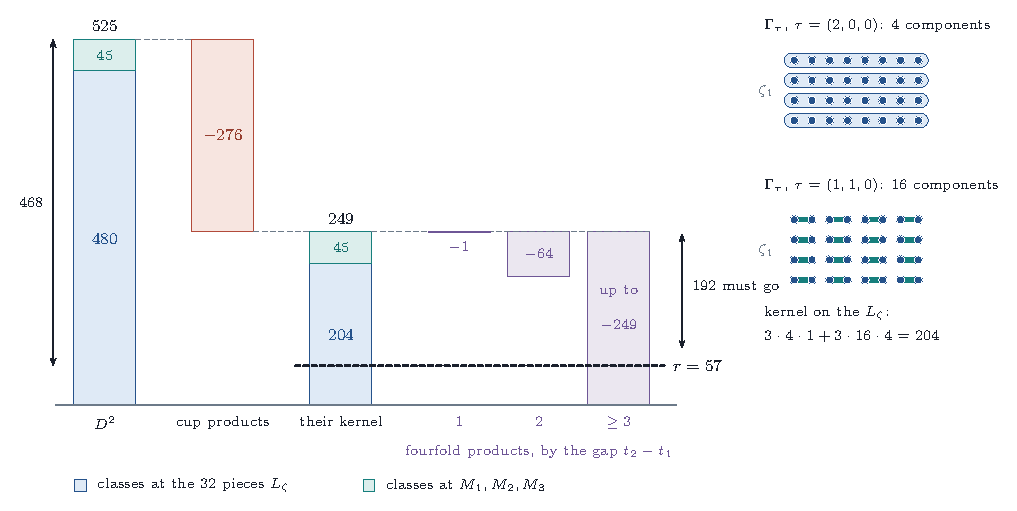
\includegraphics[width=\textwidth]{fig_diagonalbudget}
\caption{The $525$ diagonal classes of degree two at $n=3$
(\Cref{prop:cupkernel,thm:esixdiagonal}). The cup products remove $276$ of
them for general components, and at most that many in any case, leaving
$204$ at the pieces $L_{\zeta}$ and the $45$ at the $M_{i}$; when the $t_{i}$
lie on one side of $p$, the fourfold products of the surviving path remove
at most $(t_{2}-t_{1})^{6}$ more,
which is $1$ or $64$ for the gaps $1$ and $2$ and no constraint from the
third gap on. The criterion asks for $57$, so $468$ classes must disappear
in all and $192$ after the cup products. On the right, the graphs
$\Gamma_{\tau}$ on the $32$ pieces, one row for each value of $\zeta_{1}$:
for $\tau=(2,0,0)$ each row is a component, for $\tau=(1,1,0)$ the
components are the pairs differing in the sign of $\zeta_{3}$; a class
constant on the components of every $\Gamma_{\tau}$ has vanishing cup
products.}
\label{fig:diagonalbudget}
\end{figure}

The placements of the $t_{i}$ on both sides of $p$ are not covered by
\Cref{thm:esixdiagonal}. There two families of fourfold products occur
instead of one, and no convolution carries both.

\begin{proposition}[Placements on both sides of $p$]\label{prop:mixedplacement}
Keep \Cref{thm:esixdiagonal}, but let $t_{1}\le p-2$ and
$p+2\le t_{2}<t_{3}$.
\begin{enumerate}[label=\textup{(\roman*)},leftmargin=2.6em,itemsep=2pt]
\item The Massey products of length at least three vanish on $D^{2}$ unless
  $\sigma_{1}=\sigma_{2}=-\sigma_{3}$. In that case the only ones that act
  have length four and run along one of the paths
  \[
    \textup{(a)}\ \ M_{2}\to M_{3}\to M_{1}\to L_{\zeta},
    \qquad
    \textup{(b)}\ \ M_{3}\to M_{1}\to L_{\zeta}\to M_{2},
  \]
  taken in this order in the convolution, with $\prod\zeta=\sigma_{3}$. The
  products along (a) take values in $\cH^{6}(M_{2},L_{\zeta})$, of dimension
  $\bigl((t_{2}-p)^{2}-1\bigr)^{3}$, and those along (b) in
  $\cH^{6}(M_{3},M_{2})$, of dimension $(t_{3}-t_{2})^{6}$. A convolution
  carries at most one of the two kinds, since (a) puts $M_{2}$ before $M_{3}$
  and (b) puts $M_{3}$ before $M_{2}$.
\item If $E$ meets the polarised criterion, then
  $\sigma_{1}=\sigma_{2}=-\sigma_{3}$, and the products along (a) or those
  along (b) have rank at least $192$ on the kernel of the cup products. For
  (b) this needs $t_{3}-t_{2}\ge3$. The sixteen targets of (a) have
  dimension $16\bigl((t_{2}-p)^{2}-1\bigr)^{3}\ge432$, so for (a) the
  count gives no condition.
\end{enumerate}
For $t_{1}<t_{2}\le p-2$ and $t_{3}\ge p+2$ the same holds for
$E^{\vee}[1]$, and the condition on the signs becomes
$\sigma_{2}=\sigma_{3}=-\sigma_{1}$.
\end{proposition}

\begin{proof}
(i) We use the notation and the two observations of the proof of
\Cref{thm:esixdiagonal}(i). Now $\phi(M_{1})=t_{1}<p<t_{2}<t_{3}$; a step up
ends at $M_{2}$, at $M_{3}$, or at an $L_{\zeta}$ coming from $M_{1}$, so
again $U\le3$ and $D\le1$. If $D=0$, the values do not decrease along the
chain. When $e$ lies above $s$, $\varepsilon=-3$ forces $U=3$, $\lambda=0$
and the chain $M_{1}\to L_{\zeta}\to M_{2}\to M_{3}$, removed at
$L_{\zeta}\to M_{2}\to M_{3}$, the only chain of excess $-2$ from
$L_{\zeta}$ to $M_{3}$. When $e$ and $s$ have the same value, they are two
$L_{\zeta}$ joined by steps between $L_{\zeta}$, which is excluded as before.
If $D=1$, $(U,\lambda)$ is $(2,0)$, $(3,0)$ or $(3,1)$. For
$\varepsilon=3$, $e$ lies below $s$. With $(3,1)$ the steps up end at
$M_{2}$, $M_{3}$ and an $L_{\zeta}$ following $M_{1}$; then $s$ is an
$L_{\zeta}$, so $e=M_{1}$, which is followed by a step: impossible. With
$(2,0)$ the chain has three steps and no two consecutive $L_{\zeta}$. As
$M_{1}$ is the lowest piece, it is never the end of a step up, and a step up
into an $L_{\zeta}$ comes from $M_{1}$; so two consecutive steps up end at
$M_{2}$ or $M_{3}$. The chain cannot start at $M_{1}$. If it starts at an
$L_{\zeta}$, it ends at $M_{1}$ with the step down, after two steps up:
$L_{\zeta}\to M_{2}\to M_{3}\to M_{1}$, removed at $L_{\zeta}\to M_{2}\to
M_{3}$. If it starts at $M_{3}$, the first step goes down and the last two
go up, ending at $M_{2}$; the middle piece is then an $L_{\zeta}$ entered
from $M_{1}$, and the chain is $M_{3}\to M_{1}\to L_{\zeta}\to M_{2}$, path
(b). If it starts at $M_{2}$, then $e\in\{L_{\zeta},M_{1}\}$, so the last two
steps are not both up; the first step goes up to $M_{3}$, the second down,
and the third up into $e=L_{\zeta}$ from $M_{1}$: the chain is $M_{2}\to
M_{3}\to M_{1}\to L_{\zeta}$, path (a). For $\varepsilon=2$,
$(U,\lambda)=(3,0)$ and $s$, $e$ are $L_{\zeta}$ differing in one
coordinate. The last step enters $e$ from $M_{1}$, since a step down into
$e$ would follow three steps up from $s$, one more than the values allow;
$M_{1}$ is entered by the step down, after two steps up from $s$:
$L_{\zeta}\to M_{2}\to M_{3}\to M_{1}\to L_{\zeta'}$, removed at
$L_{\zeta}\to M_{2}\to M_{3}$.
Along (a) the steps have $\Ext$ degrees $0$, $6$ and $0$, so degree one
forces $d_{M_{3}}=d_{M_{2}}+1$, $d_{M_{1}}=d_{M_{3}}-5$ and
$d_{L}=d_{M_{1}}+1$. Along (b) they have $\Ext$ degrees $6$, $0$ and $0$,
which forces $d_{M_{1}}=d_{M_{3}}-5$, $d_{L}=d_{M_{1}}+1$ and
$d_{M_{2}}=d_{L}+1$. This gives the signs and puts the values in
$\cH^{3+d_{M_{2}}-d_{L}}(M_{2},L_{\zeta})=\cH^{6}(M_{2},L_{\zeta})$ and in
$\cH^{3+d_{M_{3}}-d_{M_{2}}}(M_{3},M_{2})=\cH^{6}(M_{3},M_{2})$. On $B_{j}$
the line bundle $L_{\zeta}\otimes M_{2}^{-1}$ has the hermitian form
$\bigl(\begin{smallmatrix}p-t_{2}&\zeta_{j}\\ \bbar\zeta_{j}&p-t_{2}
\end{smallmatrix}\bigr)$, with eigenvalues $p-t_{2}\pm1<0$ and determinant
$(t_{2}-p)^{2}-1$, which gives the first dimension. The second is that of
\Cref{thm:esixdiagonal}(i) with $t_{3}$, $t_{2}$ in place of $t_{2}$,
$t_{1}$.
(ii) \Cref{prop:nothingenters,prop:cupkernel} do not depend on the
placement of the $t_{i}$, so as in \Cref{thm:esixdiagonal}(ii)
$\dim\Ext^{2}(E,E)\ge249-\rho$, where $\rho$ is the rank on the kernel of
the cup products of the products of (i) that $E$ carries, and $\rho=0$
unless $\sigma_{1}=\sigma_{2}=-\sigma_{3}$. The criterion asks for $57$,
so $\rho\ge192$, and $(t_{3}-t_{2})^{6}\ge192$ exactly when
$t_{3}-t_{2}\ge3$. For the last statement, $E\mapsto E^{\vee}[1]$ preserves
$\Ext^{2}$, sends $p$ and the $t_{i}$ to $-p$ and the $-t_{i}$, reverses the
order of the pieces and changes every sign.
\end{proof}

The Maurer--Cartan equation can be solved for one order of the pieces.

\begin{proposition}[An explicit convolution]\label{prop:explicitconvolution}
Keep \Cref{thm:esixdiagonal} with $p=0$ and $t=(2,5,6)$, take the pieces to
be external products $L_{\zeta}=N_{1,\zeta_{1}}\boxtimes N_{2,\zeta_{2}}
\boxtimes N_{3,\zeta_{3}}$ and $M_{i}=M_{i,1}\boxtimes M_{i,2}\boxtimes
M_{i,3}$ of line bundles on the $B_{j}$, and order them as $M_{2}$, $M_{3}$,
the sixteen $L_{\zeta}$ with $\prod\zeta=1$, $M_{1}$, the sixteen $L_{\zeta}$
with $\prod\zeta=-1$, with the shifts $0$, $1$, $-4$, $-3$, $-5$.
\begin{enumerate}[label=\textup{(\roman*)},leftmargin=2.6em,itemsep=2pt]
\item The components that the degrees allow are
  $x_{1}\in\cH^{0}(M_{2},M_{3})$, $x_{2}^{\zeta}\in\cH^{6}(M_{3},L_{\zeta})$,
  $x_{3}^{\zeta}\in\cH^{0}(L_{\zeta},M_{1})$, components in
  $\cH^{2}(L_{\zeta},L_{\zeta'})$ for the $48+96$ pairs with
  $\prod\zeta=1=-\prod\zeta'$ that differ in one or two coordinates, and
  components in $\cH^{6}(M_{2},L_{\zeta'})$, $\prod\zeta'=-1$, which we take
  to be zero. For harmonic components the Maurer--Cartan equation is exactly
  \[
    x_{1}x_{2}^{\zeta}=0\ \text{in}\ H^{6}(A,M_{2}^{-1}\otimes L_{\zeta})
    \ \text{for every}\ \zeta,
    \qquad
    \sum_{\zeta}x_{2}^{\zeta}x_{3}^{\zeta}=0\ \text{in}\
    H^{6}(A,M_{3}^{-1}\otimes M_{1}),
  \]
  and every solution is the harmonic part of a convolution $E$ with
  $\ch(E)=32(\alpha+\bbar\alpha)+e^{5\theta}-e^{6\theta}-e^{2\theta}$.
\item There are solutions with every $x_{2}^{\zeta}\ne0$ and
  $x_{1}x_{2}^{\zeta}=x_{2}^{\zeta}x_{3}^{\zeta}=0$.
\item For every solution $\dim\Ext^{2}(E,E)\ge2560$, so $E$ does not meet
  the polarised criterion.
\end{enumerate}
\end{proposition}

\begin{proof}
(i) A component from $P_{a}$ to $P_{b}$ has $\Ext$ degree $1+d_{a}-d_{b}$, and
the forms give the cohomology of each pair: $\cH(M_{2},M_{3})$ and
$\cH(L_{\zeta},M_{1})$ sit in degree $0$, $\cH(M_{3},L_{\zeta})$,
$\cH(M_{2},L_{\zeta'})$ and $\cH(M_{2},M_{1})$ in degree $6$, and
$\cH(L_{\zeta},L_{\zeta'})$ in degree $2$ exactly for the pairs listed; no
other pair has cohomology in the degree a component needs. Put
$\delta=\delta^{H}-h(\delta\circ\delta)$ recursively, as in
\Cref{lem:harmonicmodel}(i), and $\Phi=\bar\partial\delta+\delta\circ\delta$.
Then $\Phi=\pi(\delta\circ\delta)+h\bar\partial(\delta\circ\delta)$ and
$\bar\partial(\delta\circ\delta)=\Phi\circ\delta-\delta\circ\Phi$, so by
induction on $b-a$ the twisted complex exists exactly when
$\pi(\delta\circ\delta)=0$. The components of $\pi(\delta\circ\delta)$ come
from paths of two or more components; those that land in a nonzero group
are $x_{1}x_{2}^{\zeta}$ in $\cH^{6}(M_{2},L_{\zeta})$ and
$\sum_{\zeta}x_{2}^{\zeta}x_{3}^{\zeta}$ in $\cH^{6}(M_{3},M_{1})$, while the
product along $M_{2}\to M_{3}\to L_{\zeta}\to M_{1}$ would lie in
$\cH^{5}(M_{2},M_{1})=0$ and $x_{2}^{\zeta}$ composed with a component in
$\cH^{2}(L_{\zeta},L_{\zeta'})$ in degree eight. The signs
$(-1)^{d}$ are $+,-,+,-,-$, which gives the Chern character by
\Cref{prop:weilpieces}(i).
(ii) Take $x_{1}$ and the $x_{3}^{\zeta}$ to be external products of
nonzero sections on the $B_{j}$. On each $B_{j}$ the products with their
factors map $H^{2}(B_{j},M_{3}^{-1}L_{\zeta})$, of dimension $35$, to spaces
of dimensions $24$ and $16$, so they have kernels of dimensions at least $11$
and $19$. A sum of external products whose factor on one surface lies in the
first kernel and whose factor on another lies in the second is a nonzero
$x_{2}^{\zeta}$ with $x_{1}x_{2}^{\zeta}=x_{2}^{\zeta}x_{3}^{\zeta}=0$, which
solves (i).\footnote{Such solutions are far from unique: the equations of
(i) are linear in each of $x_{1}$, $x_{2}^{\zeta}$, $x_{3}^{\zeta}$
separately, and the components on the $144$ pairs do not enter them at
all.}
(iii) The sixteen $L_{\zeta}$ with $\prod\zeta=1$ have shift $-4$ and the
others $-5$, so \Cref{lem:allthree} below applies to every pair of them
that differ in all three coordinates: there are $112$ such pairs, and their
groups $\cH^{3}$ have dimensions adding up to $16\cdot160=2560$.
\end{proof}

The classes counted in (iii) are the ones no product can reach. Two pieces
$L_{\zeta}$, $L_{\zeta'}$ that differ in every coordinate have a difference
that is indefinite on every surface, so $\cH(L_{\zeta},L_{\zeta'})$ is
$\bigotimes_{j}H^{1}(B_{j},\cdot)$, concentrated in degree three, of
dimension $D(\zeta,\zeta')=\prod_{j}|\zeta_{j}-\zeta'_{j}|^{2}$; no component
can join them, and if their shifts differ by one their classes have degree
two.

\begin{lemma}[Pieces that differ everywhere]\label{lem:allthree}
Keep \Cref{prop:nothingenters} with $n=3$. Suppose that for some integer $r$
either $p+2\le t_{1}<t_{2}<t_{3}$ and $M_{1}$, $M_{2}$, $M_{3}$ have the
shifts $r+1$, $r+4$, $r+5$, or $t_{1}\le p-2<p+2\le t_{2}<t_{3}$ and they
have the shifts $r-1$, $r+3$, $r+4$ or $r-1$, $r+1$, $r+4$; these are the
shifts forced by the paths of \Cref{thm:esixdiagonal}(i) and of
\Cref{prop:mixedplacement}(i), (a) and (b), with $r$ the shift of the
$L_{\zeta}$ on the path. Let $L_{\zeta}$, $L_{\zeta'}$ differ in all three
coordinates, with $d_{L_{\zeta}}=d_{L_{\zeta'}}+1$. Then $d_{E}$ vanishes on
$\cH^{3}(L_{\zeta},L_{\zeta'})$, and no element of degree one has a
differential with a nonzero component there. Consequently
\[
  \dim\Ext^{2}(E,E)\;\ge\;\dim\ker\bigl(d_{E}|_{D^{2}}\bigr)
  +\sum D(\zeta,\zeta'),
\]
the sum running over the pairs of this kind.
\end{lemma}

\begin{proof}
Only the shifts are used, and the order of the pieces only removes
components, so we ignore it. A component from $P_{a}$ to $P_{b}$ of $\Ext$
degree $q$ has $d_{b}=d_{a}+1-q$. Between distinct $L_{\zeta}$ the degree $q$
is at least $2$: there is no $\cH^{0}$, and $\cH^{1}$ occurs only for pieces
differing in one coordinate, which have opposite parities, while $q=1$ would
need equal shifts. So a component between two $L_{\zeta}$ lowers the shift
by at least one, and by exactly one only in degree two. For a multiple
$M_{i}$ let $\mu_{i}$ and $\nu_{i}$ be the shifts of an $L_{\zeta}$ that a
component from $M_{i}$ reaches and from which a component reaches $M_{i}$:
$\mu_{i}=d_{M_{i}}-5$ and $\nu_{i}=d_{M_{i}}-1$ when $t_{i}>p$, and
$\mu_{i}=d_{M_{i}}+1$, $\nu_{i}=d_{M_{i}}+5$ when $t_{i}<p$. Between the
multiples the degrees allow only $M_{2}\to M_{3}$ in the first case,
$M_{2}\to M_{3}\to M_{1}$ in the second, and $M_{3}\to M_{1}$ in the third.
Let $\lambda_{i}$ be the largest $\mu_{k}$ and $\kappa_{i}$ the least
$\nu_{k}$ over the multiples $M_{k}$ reachable from $M_{i}$, respectively
reaching $M_{i}$, through these steps, $M_{i}$ included. The values, in the
order $M_{1}$, $M_{2}$, $M_{3}$ and relative to $r$, are
\[
\begin{array}{l|ccc|ccc|ccc|ccc}
 & \multicolumn{3}{c|}{\mu} & \multicolumn{3}{c|}{\nu}
 & \multicolumn{3}{c|}{\lambda} & \multicolumn{3}{c}{\kappa}\\
\hline
r+1,\,r+4,\,r+5 & -4&-1&0 & 0&3&4 & -4&0&0 & 0&3&3\\
r-1,\,r+3,\,r+4 & 0&-2&-1 & 4&2&3 & 0&0&0 & 2&2&2\\
r-1,\,r+1,\,r+4 & 0&-4&-1 & 4&0&3 & 0&-4&0 & 3&0&3
\end{array}
\]
and in all three cases, for all $i$ and $k$,
\begin{equation}\label{eq:allthree}
  \lambda_{i}\le r\le\kappa_{k},\qquad
  \kappa_{i}\ge\lambda_{i}+2,\qquad
  \lambda_{i}\le\mu_{i}+2,\qquad
  \nu_{i}\le\kappa_{i}+2,
\end{equation}
while $\mu_{i}\le\lambda_{i}$ and $\nu_{i}\ge\kappa_{i}$ by definition. A
run $L\to M_{k}\to\dots\to M_{i}\to L'$ through multiples goes from the shift
$\nu_{k}\ge\kappa_{k}$ to $\mu_{i}\le\lambda_{k}\le\kappa_{k}-2$, so every chain
of components from one $L$ to another lowers the shift, by at least two if it
passes through a multiple and by exactly one only if it is a single component
of degree two. In particular a chain from an $L$ of shift $x$ into $M_{i}$
has $x\ge\kappa_{i}$, and a chain from $M_{i}$ to an $L$ of shift $y$ has
$y\le\lambda_{i}$.

By \Cref{lem:harmonicmodel}(iii), a term of $d_{E}$ on a class $u$ of $\Ext$
degree $q_{u}$ in $\cH(a',b')$ runs along a chain $c\to\dots\to a'$, the
step $u$, and a chain $b'\to\dots\to e$, and since the degrees of the
components telescope, its value lies in $\cH(c,e)$ in $\Ext$ degree
\[
  q_{u}+1+(d_{c}-d_{a'})+(d_{b'}-d_{e}).
\]
Write $a=L_{\zeta}$ and $b=L_{\zeta'}$, so that $d_{a}=d_{b}+1$.

\emph{Nothing reaches $\cH^{3}(a,b)$.} Let $u$ have degree one, so
$q_{u}=1+d_{a'}-d_{b'}$, with chains from $a$ to $a'$ and from $b'$ to $b$
and $(a',b')\ne(a,b)$. If $a'$ and $b'$ are both pieces $L$, then
$d_{a'}\le d_{a}$ and $d_{b'}\ge d_{b}$, not both with equality, so
$q_{u}\le1$; $q_{u}=0$ is impossible, and $q_{u}=1$ needs either $a'=b'$, and
then a chain from $a$ to $b$ lowering the shift by one, a single component in
$\cH^{2}(a,b)=0$, or $a'$, $b'$ differing in one coordinate, of opposite
parities, against $d_{a'}=d_{b'}$. If $a'=M_{i}$ and $b'$ is an $L$, then
$u$ lies in the degree of a component, so $d_{b'}=\mu_{i}$, while
$d_{b'}\ge d_{b}=d_{a}-1\ge\kappa_{i}-1\ge\lambda_{i}+1>\mu_{i}$. If $a'$ is
an $L$ and $b'=M_{k}$, then $d_{a'}=\nu_{k}$ and
$d_{a}-d_{b}\ge\nu_{k}-\lambda_{k}\ge\kappa_{k}-\lambda_{k}\ge2$. If
$a'=M_{i}$ and $b'=M_{k}$, then $d_{a}-d_{b}\ge\kappa_{i}-\lambda_{k}$; for
$i=k$ this is at least $2$, and for $i\ne k$ the class $u$ lies in the
degree of a step $M_{i}\to M_{k}$, so $\lambda_{k}\le\lambda_{i}$ and again
$d_{a}-d_{b}\ge2$. Each case contradicts $d_{a}-d_{b}=1$.

\emph{$d_{E}$ vanishes on $\cH^{3}(a,b)$.} Here $u$ is the class itself and a
term lands in $\cH(c,e)$, $(c,e)\ne(a,b)$, in degree $3+d_{c}-d_{e}$, with
chains from $c$ to $a$ and from $b$ to $e$. If $c$ and $e$ are both pieces
$L$, then $d_{c}-d_{e}\ge2$; $c=e$ is impossible, and otherwise a class of
degree at least $5$ needs $c$, $e$ differing in one coordinate, in degree
$5$, so $d_{c}-d_{e}=2$ against their opposite parities. If $c=M_{i}$ and
$e$ is an $L$, the degree is that of a component when $d_{e}=\mu_{i}+2$, but
$d_{e}\le d_{b}<d_{a}\le\lambda_{i}\le\mu_{i}+2$. If $c$ is an $L$ and
$e=M_{k}$, it is that of a component when $d_{c}=\nu_{k}-2$, but
$d_{c}\ge d_{a}>d_{b}\ge\kappa_{k}\ge\nu_{k}-2$. If $c=M_{i}$ and
$e=M_{k}$, then $d_{a}\le\lambda_{i}\le r\le\kappa_{k}\le d_{b}$, against
$d_{a}>d_{b}$.

For the inequality: a coboundary has no component on $D^{2}$
(\Cref{prop:nothingenters}) and none on these groups, so the cocycles of
$\ker(d_{E}|_{D^{2}})$ and of these groups span a space that meets the
coboundaries only in zero. Twisting the pieces by line bundles of degree
zero does not change $D(\zeta,\zeta')$, the forms being nondegenerate on
every surface, and can only remove components.
\end{proof}

\begin{theorem}[No convolution of these pieces meets the criterion]
\label{thm:noconvolution}
Keep \Cref{prop:nothingenters} with $n=3$: let $E$ be any convolution of
the $32$ bundles $L_{\zeta}$ and of $M_{1}$, $M_{2}$, $M_{3}$, with
$t_{1}<t_{2}<t_{3}$ and $|t_{i}-p|\ge2$, in any order, with any shifts of the
given parities and with the pieces twisted by any line bundles of degree
zero. Then $\dim\Ext^{2}(E,E)\ge69$. In particular no such convolution meets
the polarised criterion, which asks for $57$.
\end{theorem}

\begin{proof}
Replacing $E$ by $E^{\vee}$ or $E^{\vee}[1]$, which preserves $\Ext^{2}$, we
may assume that the $t_{i}$ are as in \Cref{thm:esixdiagonal} or in
\Cref{prop:mixedplacement}. If no fourfold product of those results acts,
$\dim\Ext^{2}(E,E)\ge249$. Otherwise the path fixes the shifts of the
$M_{i}$ as in \Cref{lem:allthree}, with $r$ the shift of every $L_{\zeta}$
on a path; let $P$ be the sixteen pieces of the parity of $r$, $Q$ the
other sixteen, and $m$ the number of pieces on paths.

The fourfold products act on $D^{2}$ only through the classes at the
$M_{i}$ and at the $m$ pieces on paths, so their rank is at most $45+15m$,
and by \Cref{prop:cupkernel}
$\dim\ker(d_{E}|_{D^{2}})\ge249-45-15m=204-15m$. If $m\le9$ this is at
least $69$.

Let $m\ge10$, so that at least ten pieces of $P$ have the shift $r$. Every
$W\in Q$ has $3$, $6$ and $7$ partners in $P$ differing from it in one, two
and three coordinates, and for the seven $D=16$ six times and $D=64$
once.\footnote{The ratios $\zeta'_{j}/\zeta_{j}$ of two pieces of opposite
parities have product $-1$; when all three differ from $1$ they are
$(-1,-1,-1)$, with $D=4^{3}$, or a permutation of $(i,-i,-1)$, with
$D=2\cdot2\cdot4$.} If $d_{W}=r\pm1$, at most six pieces of $P$ lack the
shift $r$, so one of the seven has it, and \Cref{lem:allthree} gives at least
$16$ classes. If $d_{W}\ne r\pm1$, consider for each type $\tau$ of the form
$(1,1,0)$ the partner $W^{\tau}\in P$ obtained by changing the sign of the
coordinate where $\tau$ vanishes. By the proof of \Cref{prop:cupkernel},
$W^{\tau}$ is the only piece with which $W$ can carry a nonzero cup product
on the type $\tau$, and conversely; a cup product between them needs a
component of degree two, hence shifts differing by one. If they do, the
classes of type $\tau$ equal at $W$ and $W^{\tau}$ and zero elsewhere have
vanishing cup products, and $W^{\tau}$, of shift $d_{W}\pm1\ne r$, lies on no
path; if they do not, the classes of type $\tau$ at $W$ alone have vanishing
cup products. Either way these $4$ classes lie in $\ker(d_{E}|_{D^{2}})$,
$12$ for each such $W$, and those of different $W$ are independent, since
$W\mapsto W^{\tau}$ is injective. Adding over $Q$, \Cref{lem:allthree}
gives $\dim\Ext^{2}(E,E)\ge16\cdot12=192$.
\end{proof}

At $n=4$ there are $128$ pieces $L_{\zeta}$, and the classes that no
product reaches are again those between pieces that differ in three
coordinates and have adjacent shifts. The shifts along a chain are now
controlled by counting alone.

\begin{lemma}[Shifts along chains at $n=4$]\label{lem:efourshifts}
Keep \Cref{prop:weilpieces} with $n=4$, take the $L_{\zeta}$ to be external
products $N_{1,\zeta_{1}}\boxtimes\dots\boxtimes N_{4,\zeta_{4}}$ of line
bundles on the $B_{j}$, let $t_{1},t_{2},t_{3}$ be distinct with
$|t_{i}-p|\ge2$, and let $E$ be a convolution of the $L_{\zeta}$ and of
$M_{1},M_{2},M_{3}$ with shifts of the given parities. Call a component of
$\delta^{H}$, or an element of degree one of $\cH_{E}$ in one group
$\cH(a,b)$, a step from $P_{a}$ to $P_{b}$; a step of $\Ext$ degree $q$ has
$d_{b}=d_{a}+1-q$. Put $\phi(L_{\zeta})=p$ and $\phi(M_{i})=t_{i}$.
\begin{enumerate}[label=\textup{(\roman*)},leftmargin=2.6em,itemsep=2pt]
\item A step between distinct $L_{\zeta}$ has $\Ext$ degree at least two, so
  it lowers the shift by at least one, and by exactly one only in $\Ext$
  degree two. A step in $\cH^{1}(a,a)=H^{1}(A,\cO_{A})$ keeps the shift.
\item A step between an $L_{\zeta}$ and a multiple, or between two
  multiples, has $\Ext$ degree $0$ if it goes up the value $\phi$ and $8$ if
  it goes down, so it raises the shift by one or lowers it by seven.
\item A sequence of steps from an $L_{\zeta}$ to an $L_{\zeta'}$ through
  multiples, distinct before one marked step and distinct after it, where
  the marked step may lie in $\cH^{1}(a,a)$ at a multiple, lowers the shift
  by at least four. Consequently a sequence of steps from one $L_{\zeta}$ to
  another, at most one of them not a component, lowers the shift by at least
  one, and by exactly one only if it consists of steps between pieces
  $L_{\zeta}$, one of $\Ext$ degree two and the others in $\cH^{1}(a,a)$.
\end{enumerate}
\end{lemma}

\begin{proof}
(i) For $\zeta\ne\zeta'$ the group $\cH(L_{\zeta},L_{\zeta'})$ is the tensor
product over the surfaces of $H^{1}$ of a line bundle with a nondegenerate
form, on the $k\ge1$ surfaces where $\zeta$ and $\zeta'$ differ, and of
$H^{*}(B_{j},\cO_{B_{j}})$ on the others, the factors of $L_{\zeta}$ and
$L_{\zeta'}$ on those being equal. So its degrees are at least $k$, and degree
one needs $k=1$. Then the ratio $\zeta'_{j}/\zeta_{j}\ne1$ in the one
coordinate is the ratio of $\prod\zeta'$ and $\prod\zeta$, which is $-1$, and
the shifts have opposite parities, while a step of $\Ext$ degree one keeps
the shift. (ii) The forms of $M_{i}\otimes L_{\zeta}^{-1}$ have the
eigenvalues $t_{i}-p\pm1$ on every surface, which have the sign of $t_{i}-p$;
the form of $M_{k}\otimes M_{i}^{-1}$ is $(t_{k}-t_{i})\,\mathrm{Id}$. A
definite form has cohomology in degree $0$ if it is positive and $2n=8$ if
it is negative \cite[Chapter~3]{BL04}.%
\footnote{This is Mumford's index theorem: a line bundle on an abelian
variety whose hermitian form is nondegenerate with $i$ negative eigenvalues
has cohomology only in degree $i$. On $B_{j}=E_{0}\times E_{0}$ the form of
$M_{i}\otimes L_{\zeta}^{-1}$ is
$\bigl(\begin{smallmatrix}t_{i}-p&-\zeta_{j}\\-\bar\zeta_{j}&t_{i}-p\end{smallmatrix}\bigr)$,
with eigenvalues $t_{i}-p\pm1$, and $|t_{i}-p|\ge2$ makes both of the sign of
$t_{i}-p$; over the four surfaces the index is $0$ or $8$. The hypothesis
$|t_{i}-p|\ge2$ is what keeps the steps between a piece and a multiple out
of the middle degrees.}
(iii) Let $U$ and $D$ be the numbers of steps up and down outside
$\cH^{1}(a,a)$; by (ii) the shift changes by $U-7D$. The values start and
end at $p$ and pass through the values of multiples, so $D\ge1$. If $D=1$,
the values increase strictly before the step down and strictly after it, so
those before it lie above $p$ and those after it below $p$, each multiple
occurs once, and $U\le3$: the drop $7-U$ is at least four.%
\footnote{The bound is attained: with $p$ below the three values $t_{i}$, the
run $L_{\zeta}\to M_{1}\to M_{2}\to M_{3}\to L_{\zeta'}$, up three times and
down once, changes the shift by $3-7=-4$. With $p$ in the middle,
$t_{1}<p<t_{2}<t_{3}$, the run up through $M_{2}$ and $M_{3}$, down to $M_{1}$
and up to $L_{\zeta'}$ changes it by $3-7=-4$ as well.} If $D\ge2$, at most
six multiples occur, counted with repetition, so there are at most seven
steps outside $\cH^{1}(a,a)$, $U\le7-D$, and the drop $7D-U\ge8D-7$ is at
least nine. For the consequence, split the sequence at the pieces
$L_{\zeta}$ it visits: each part through multiples lowers the shift by at
least four, and by (i) each other part lowers it by at least one, unless it
lies in $\cH^{1}(a,a)$.
\end{proof}

\begin{theorem}[Two shifts on $E_{0}^{8}$]\label{thm:efourtwolevels}
Keep \Cref{lem:efourshifts}, and let $L_{\zeta}$ and $L_{\zeta'}$ differ in
exactly three coordinates and have the shifts $d_{L_{\zeta}}=d_{L_{\zeta'}}+1$.
Then $\cH(L_{\zeta},L_{\zeta'})$ has its classes of degree two in
$\cH^{3}(L_{\zeta},L_{\zeta'})$, of dimension
$D(\zeta,\zeta')=\prod_{\zeta_{j}\ne\zeta'_{j}}|\zeta_{j}-\zeta'_{j}|^{2}$,
which is $16$ or $64$, and:
\begin{enumerate}[label=\textup{(\roman*)},leftmargin=2.6em,itemsep=2pt]
\item for every convolution, no element of degree one has a differential
  with a nonzero component in $\cH^{3}(L_{\zeta},L_{\zeta'})$;
\item if the $L_{\zeta}$ occupy two consecutive shifts, those with
  $\prod\zeta=\epsilon$ the shift $s$ and the others $s-1$, for a sign
  $\epsilon$ and an integer $s$, then $d_{E}$ vanishes on these groups, and
  for every order of the pieces, every choice of the shifts of the $M_{i}$
  and every placement of the $t_{i}$,
  \[
    \dim\Ext^{2}(E,E)\;\ge\;64\cdot640=40960 .
  \]
  In particular $E$ does not meet the polarised criterion, which asks for
  $\dim\Ext^{2}(E,E)=104$.
\end{enumerate}
\end{theorem}

\begin{proof}
Write $W=L_{\zeta}$ and $V=L_{\zeta'}$. By the proof of
\Cref{lem:efourshifts}(i), $\cH(W,V)$ has degrees $3$, $4$ and $5$, the last
two from the surface where $\zeta$ and $\zeta'$ agree, and its classes of
degree $w=2$ have $\Ext$ degree $2+d_{W}-d_{V}=3$; the dimension of
$\cH^{3}(W,V)$ is the product over the three other surfaces of the
determinants $|\zeta_{j}-\zeta'_{j}|^{2}$, as in \Cref{lem:allthree}.

(i) As in the proof of \Cref{lem:allthree}, a term of the differential of an
element $u$ of degree one in $\cH(a',b')$ with a component in $\cH(W,V)$
runs along a chain of components $W\to\dots\to a'$, the step $u$, and a chain
$b'\to\dots\to V$, with $(a',b')\ne(W,V)$. This is a sequence of steps from
$W$ to $V$, one of them $u$, lowering the shift by one. By
\Cref{lem:efourshifts}(iii) it consists of steps between pieces $L_{\zeta}$,
one of $\Ext$ degree two and at most one, $u$, in $\cH^{1}(a,a)$. If $u$ is
not in $\cH^{1}(a,a)$, it is the step of degree two and both chains are
empty, against $(a',b')\ne(W,V)$. If $u$ is in $\cH^{1}(a,a)$, the rest is a
single component $W\to V$ of $\Ext$ degree two, in $\cH^{2}(W,V)=0$.

(ii) A term of $d_{E}$ on $x\in\cH^{3}(W,V)$ runs along chains of components
$c\to\dots\to W$ and $V\to\dots\to e$, not both empty, and lands in $\cH(c,e)$
in $\Ext$ degree $3+1+(d_{c}-d_{W})+(d_{V}-d_{e})=3+d_{c}-d_{e}$. No piece
$L_{\zeta''}$ other than $W$ lies on the first chain: by
\Cref{lem:efourshifts}(iii) it would have the shift at least $d_{W}+1=s+1$.
Likewise only multiples follow $V$ on the second chain, and each chain has at
most three pieces besides $W$ or $V$. Let $U$ and $D$ be the numbers of steps
up and down along both chains, so that $U+D\le6$; by
\Cref{lem:efourshifts}(ii), $d_{W}=d_{c}+U_{1}-7D_{1}$ and
$d_{e}=d_{V}+U_{2}-7D_{2}$, and the $\Ext$ degree is
\[
  3+d_{c}-d_{e}=4-U+7D .
\]
If $c=e$, this degree is $3$, so $U=7D+1$, and $D\ge1$ because the values
return to $\phi(c)\ne p$; then $U\ge8$, which is impossible. If $c\ne e$, the
group $\cH(c,e)$ sits in degree $0$ if $\phi(e)>\phi(c)$ and in degree $8$ if
$\phi(e)<\phi(c)$, by \Cref{lem:efourshifts}(ii). Degree $0$ needs
$U=4+7D\ge4$ with $D=0$, so the values increase strictly, the multiples are
distinct and $U\le3$. Degree $8$ needs $7D=U+4$, so $D=1$ and $U=3$; the
values increase strictly before the step down, from $\phi(c)$, and after it,
up to $\phi(e)<\phi(c)$, so the five values along the path, with $W$ and $V$
counted once, are distinct, and four of them are values of multiples, of
which there are three. So no term reaches a nonzero group, and $d_{E}$
vanishes on $\cH^{3}(W,V)$.

By (i) and (ii) the classes of these groups are cocycles of degree two, and
no nonzero combination of them is a coboundary, since every coboundary has
zero components there. Each piece of the shift $s$ has $28$ partners of the
other parity differing from it in exactly three
coordinates,\footnote{The ratios $\zeta'_{j}/\zeta_{j}$ in the three
coordinates have product $-1$, so they are $(-1,-1,-1)$, with $D=64$, or a
permutation of $(i,-i,-1)$, with $D=16$; with four places for the
coordinate where they agree this gives $4\cdot7=28$ partners and
$4\cdot(64+6\cdot16)=640$ classes.} all of the shift $s-1$, and the $28$
groups have dimensions adding up to $640$; there are $64$ pieces of the shift
$s$.
\end{proof}

\begin{figure}[tbp]
\centering
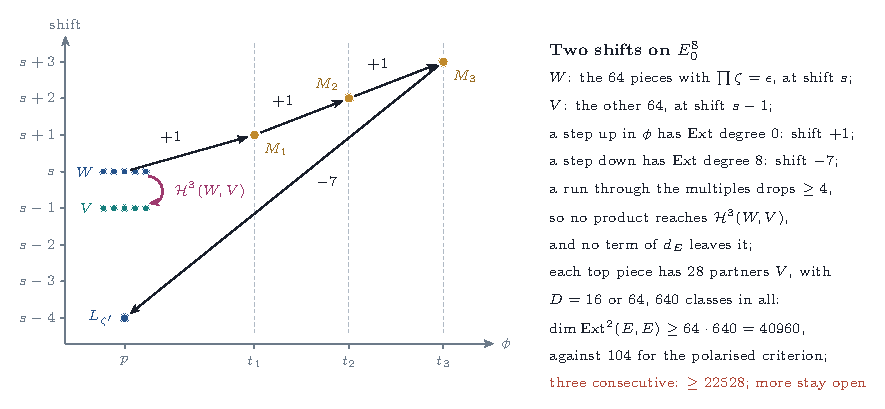
\includegraphics[width=\textwidth]{fig_efourshifts}
\caption{\Cref{lem:efourshifts} and \Cref{thm:efourtwolevels}, in the
placement $p<t_{1}<t_{2}<t_{3}$. Horizontal: the value $\phi$ of a piece;
vertical: its shift. The pieces $L_{\zeta}$ with $\prod\zeta=\epsilon$ sit at
the shift $s$ and the others at $s-1$. A run through the multiples, up three
times with $\Ext$ degree $0$ and down once with $\Ext$ degree $8$, ends four
shifts lower, the least drop of \Cref{lem:efourshifts}(iii), so it never
joins a top piece $W$ to a partner $V$ one shift lower; the group
$\mathcal{H}^{3}(W,V)$ survives in $\Ext^{2}(E,E)$.}
\label{fig:efourshifts}
\end{figure}

\Cref{fig:efourshifts} draws the shifts along a run. The hypothesis of (ii) is the arrangement of the explicit convolution of
\Cref{prop:explicitconvolution} at $n=3$, where the sixteen pieces of each
parity share a shift. The pieces
must not be twisted by line bundles of degree zero here, unlike in
\Cref{thm:noconvolution}: a twist that is nontrivial on the surface where
$\zeta$ and $\zeta'$ agree removes $\cH(L_{\zeta},L_{\zeta'})$.

With a third shift, a component of $\Ext$ degree two can follow or precede
a class of $\cH^{3}(L_{\zeta},L_{\zeta'})$, so the differential no longer
vanishes on these classes. When the three shifts are consecutive, such terms
reach only the groups
between the highest and the lowest shift, which are too small to remove the
classes.

\begin{theorem}[Three consecutive shifts on $E_{0}^{8}$]
\label{thm:efourthreelevels}
Keep \Cref{lem:efourshifts}, and suppose that the shifts of the $L_{\zeta}$
lie in $\{s,s-1,s-2\}$ for an integer $s$. By their parities, for a sign
$\epsilon$, the pieces with $\prod\zeta=\epsilon$ have the shift $s-1$ and
the others the shift $s$ or $s-2$; let $T$ and $B$ be the sets of pieces of
the shifts $s$ and $s-2$. Then, for every order of the pieces, every choice
of the shifts of the $M_{i}$ and every placement of the $t_{i}$:
\begin{enumerate}[label=\textup{(\roman*)},leftmargin=2.6em,itemsep=2pt]
\item every two pieces $L_{\zeta}$, $L_{\zeta'}$ that differ in exactly three
  coordinates have shifts differing by one, and the groups
  $\cH^{3}(L_{\zeta},L_{\zeta'})$ of \Cref{thm:efourtwolevels}, taken from
  the piece of the larger shift, have dimensions adding up to $40960$;
\item $d_{E}$ maps the sum of these groups into
  $\bigoplus_{c\in T,\,e\in B}\cH^{5}(c,e)$, and on them it consists of cup
  products with a single component of $\Ext$ degree two;
\item
  \[
    \dim\Ext^{2}(E,E)\;\ge\;40960-\sum_{c\in T,\,e\in B}\dim\cH^{5}(c,e)
    \;\ge\;40960-18432=22528 .
  \]
\end{enumerate}
In particular $E$ does not meet the polarised criterion. When $T$ or $B$ is
empty this is \Cref{thm:efourtwolevels}(ii).
\end{theorem}

\begin{proof}
(i) The ratios $\zeta'_{j}/\zeta_{j}$ in the three coordinates have
product $-1$, so the two pieces have opposite parities: one has the shift
$s-1$ and the other $s$ or $s-2$. Each of the $64$ pieces of the shift $s-1$
has $28$ such partners, whose groups have dimensions adding up to $640$, as
in the proof of \Cref{thm:efourtwolevels}; this gives $64\cdot640=40960$.

(ii) Let $x\in\cH^{3}(a,b)$ with $d_{a}=d_{b}+1$. As in the proof of
\Cref{thm:efourtwolevels}(ii), a term of $d_{E}(x)$ runs along chains of
components $c\to\dots\to a$ and $b\to\dots\to e$, not both empty, and lands
in $\cH(c,e)$ in $\Ext$ degree $3+d_{c}-d_{e}$. The shifts of the pieces
$L_{\zeta}$ differ by at most two, so by \Cref{lem:efourshifts}(iii) no part
of a chain between two pieces $L_{\zeta}$ passes through a multiple. Hence a
chain $c\to\dots\to a$ that starts at a multiple $M_{i}$ is a run
$M_{i}=m_{0}\to\dots\to m_{r}\to L_{1}$ of distinct multiples, $r\le2$,
followed by pieces $L_{\zeta}$ only; let $U_{1}$ and $D_{1}$ be the numbers
of its steps up and down the value $\phi$ before $L_{1}$, so that
$d_{L_{1}}=d_{M_{i}}+U_{1}-7D_{1}$ by \Cref{lem:efourshifts}(ii) and
$U_{1}+D_{1}=r+1\le3$. Likewise a chain $b\to\dots\to e$ ending at a multiple
$M_{k}$ ends with a run from a piece $L_{2}$ with $U_{2}$ steps up and $D_{2}$
down, $U_{2}+D_{2}\le3$ and $d_{M_{k}}=d_{L_{2}}+U_{2}-7D_{2}$. Put
$L_{1}=c$ if $c$ is a piece $L_{\zeta}$ and $L_{2}=e$ if $e$ is one, and
$\delta=d_{L_{1}}-d_{L_{2}}$; then $1=d_{a}-d_{b}\le\delta\le2$.

If $c$ and $e$ are both pieces $L_{\zeta}$, each nonempty chain lowers the
shift by at least one, so $3+d_{c}-d_{e}\ge5$, while $\delta\le2$ gives at
most $5$. So the degree is $5$, $c\in T$, $e\in B$, and the two chains
together consist of one component, of $\Ext$ degree two by
\Cref{lem:efourshifts}(i): the term is a cup product of $x$ with that
component.

If $c=M_{i}$ and $e$ is a piece $L_{\zeta}$, the degree is
$3+\delta-U_{1}+7D_{1}$, and $\cH(c,e)$ sits in degree $0$ or $8$ by
\Cref{lem:efourshifts}(ii). Degree $0$ needs $U_{1}\ge3+\delta\ge4$, and
degree $8$ needs $7D_{1}-U_{1}=5-\delta\in\{3,4\}$, so $D_{1}\ge1$ and
$U_{1}\ge3$; both contradict $U_{1}+D_{1}\le3$. The case of a piece $c$ and
a multiple $e$ is the same with the second run.

If $c=M_{i}$ and $e=M_{k}$, the degree is $3+\delta-U+7D$ with
$U=U_{1}+U_{2}\le6$ and $D=D_{1}+D_{2}$. For $i=k$ it is $3$, so
$U-7D=\delta\ge1$; $D=0$ is impossible, since the values would increase from
$t_{i}$ to $p$ along the first run and from $p$ to $t_{i}$ along the second,
and $D\ge1$ gives $U\ge8$. For $i\ne k$, $\cH(c,e)$ sits in degree $0$ if
$t_{k}>t_{i}$ and $8$ if $t_{k}<t_{i}$. Degree $0$ needs $U=3+\delta+7D$,
so $D=0$ and $U\ge4$; but then the multiples of the first run have values
below $p$ and those of the second values above $p$, so they are distinct and
$U\le3$. Degree $8$ needs $7D-U=5-\delta$, so $D=1$ and $U\ge3$: the runs
have at least four steps, so some multiple lies on both. One run increases
strictly. If it is the second, its values lie in $(p,t_{k}]$, while those of
the first lie at or above $t_{i}>t_{k}$ before its step down and below $p$
after it. If it is the first, its values lie in $[t_{i},p)$, while those of
the second lie above $p$ before its step down and at or below $t_{k}<t_{i}$
after it. Either way no multiple lies on both runs, a contradiction.

(iii) By \Cref{thm:efourtwolevels}(i), which holds for every convolution, no
coboundary has a component in these groups, so the kernel of $d_{E}$ on
their sum injects into $\Ext^{2}(E,E)$, and by (ii) its dimension is at
least $40960$ minus the dimension of the targets. For pieces $c$, $e$ of the
same parity, $\cH^{5}(c,e)$ is nonzero only when they differ in two or three
coordinates, and each piece has such partners with groups $\cH^{5}$ of
dimensions adding up to $960$.\footnote{The ratios $e_{j}/c_{j}\ne1$ have
product $1$. In two coordinates they are $(-1,-1)$, with $D=16$, or
$(i,-i)$, $(-i,i)$, with $D=4$; then
$\cH^{5}=\cH^{1}\otimes\cH^{1}\otimes\cH^{3}(B_{j}\times B_{k},\cO)$ has
dimension $4D$, and the six pairs of coordinates give
$6\cdot64+12\cdot16=576$. In three coordinates they are a permutation of
$(i,i,-1)$ or of $(-i,-i,-1)$, with $D=16$, and
$\cH^{5}=(\cH^{1})^{\otimes3}\otimes H^{2}(B_{l},\cO)$ has dimension $16$;
the four triples give $4\cdot6\cdot16=384$. In four coordinates
$\cH(c,e)$ sits in degree $4$.}\enlargethispage{3pt} So the sum in (iii) is at most
$\min(|T|,|B|)\cdot960\le32\cdot960=30720$, which already gives
$\dim\Ext^{2}(E,E)\ge10240$. The dimension of $\cH^{5}(c,e)$ depends only on
the ratio $e/c$, so the sum is the weight of the cut $(T,B)$ of a weighted
Cayley graph on the group of ratios of two pieces of one parity, of order
$64$ and degree $960$. For the vector $x=\pm1$ of the cut, the weight is
$\tfrac14\bigl(64\cdot960-x^{\mathsf T}Ax\bigr)\le16\,(960-\lambda)$, with
$A$ the weighted adjacency matrix and $\lambda$ its least eigenvalue. Its
eigenvalues are the character sums $\sum_{g}\dim\cH^{5}(1,g)\,\chi(g)$. A
character is $\chi(g)=\prod_{j}g_{j}^{k_{j}}$ with $k\in(\ZZ/4)^{4}$, up to
adding $(1,1,1,1)$; put $\omega_{j}=i^{k_{j}}$, $W=\sum_{j}\omega_{j}$,
$\varrho=\sum_{j}\omega_{j}^{2}$ and $\Omega=\prod_{j}\omega_{j}$. By the
list in the footnote, the ratios that move the pair of coordinates
$\{j,l\}$ contribute $64\,\omega_{j}^{2}\omega_{l}^{2}
+32\,\Re(\omega_{j}\bbar\omega_{l})$, and those that fix only the
coordinate $o$ contribute $32\,\Re\bigl(\Omega\bbar\omega_{o}(W-\omega_{o})\bigr)$.
Summing,
\[
  \chi\bigl(\textstyle\sum_{g}\dim\cH^{5}(1,g)\,g\bigr)
  =32\varrho^{2}+16|W|^{2}-192+32\,\Re(\Omega)\bigl(|W|^{2}-4\bigr).
\]
If $\Re\Omega=0$, the sum of the $k_{j}$ is odd, so an odd number of them
are odd, $|\varrho|=2$, and the value is at least $-64$. If $\Re\Omega=1$,
an even number are odd: with none or four, $|\varrho|=4$ and the value is at
least $192$; with two, $\varrho=0$, and $W=0$ would force the $k_{j}$ to be
$0,1,2,3$, whose sum is not divisible by $4$, so $|W|^{2}\ge4$ and the value
is at least $-128$. If $\Re\Omega=-1$, the value is
$32\varrho^{2}-16|W|^{2}-64$, and $|W|^{2}\le8+2\varrho^{2}$: when all
$k_{j}$ have the same parity, $|W|\le4=|\varrho|$, and when two are odd,
$\varrho=0$ and $W$ is a sum of two of $\pm1$ and two of $\pm i$, so
$|W|^{2}\le8$. Hence $\lambda\ge-192$,\footnote{The eight values are $960$,
$384$, $192$, $96$, $-32$, $-64$, $-128$ and $-192$. The bound $18432$ is
attained by the cut $\zeta_{3}\zeta_{4}\in\{1,i\}$ against
$\zeta_{3}\zeta_{4}\in\{-1,-i\}$, so $22528$ is the best bound that this
count gives.} and the sum is at most $16\cdot1152=18432$.
\end{proof}

\Cref{fig:efourthree} draws the three shifts and the budget.

\begin{figure}[tbp]
\centering
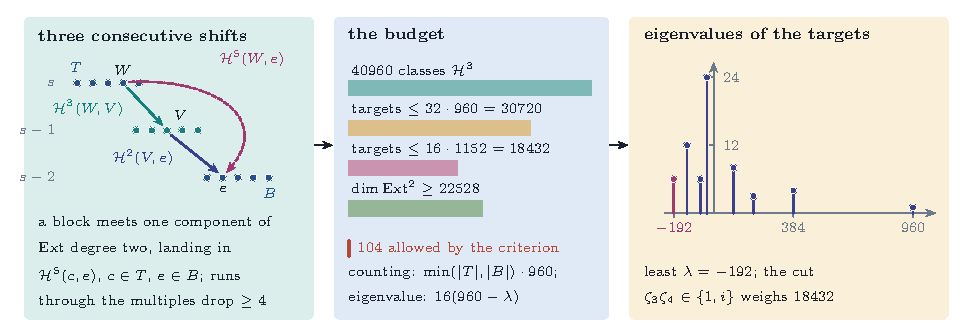
\includegraphics[width=\textwidth]{fig_efourthree}
\caption{\Cref{thm:efourthreelevels}. Left: the pieces $L_{\zeta}$ at three
consecutive shifts, those of one parity at $s-1$ and the others split between
$T$ at $s$ and $B$ at $s-2$; a group $\cH^{3}$ between two pieces that differ
in three coordinates (teal) can meet a component of $\Ext$ degree two
(indigo) only in a group $\cH^{5}(c,e)$ with $c\in T$ and $e\in B$ (magenta).
Middle: the $40960$ classes against the targets, at most $30720$ by counting
and $18432$ by the least eigenvalue, against the $104$ that the criterion
allows. Right: the eigenvalues of the Cayley graph of the targets.}
\label{fig:efourthree}
\end{figure}

The groups of \Cref{thm:efourtwolevels} join two pieces whose shifts differ
by one. All groups between pieces whose shifts differ by three, and thirteen
kinds between pieces whose shifts differ by two, are also left alone by the
differential, and with them the argument covers every
arrangement of the shifts within five consecutive values. For pieces $a$ and
$b$ call $d_{a}-d_{b}$ the \emph{spread} of $\cH(a,b)$; its classes of degree
two have $\Ext$ degree $2+d_{a}-d_{b}$. For $\zeta,\zeta'\in\mu_{4}^{4}$ call
$\zeta'/\zeta=(\zeta'_{j}/\zeta_{j})_{j}$ their \emph{ratio}; it
\emph{moves} the coordinates where it differs from $1$, and it changes the
parity, $\prod\zeta'=-\prod\zeta$, exactly when the product of its entries is
$-1$. As before,
$D(\zeta,\zeta')=\prod_{\zeta_{j}\ne\zeta'_{j}}|\zeta_{j}-\zeta'_{j}|^{2}$.

\begin{lemma}[Groups of spread two and three]\label{lem:efourspread}
Keep \Cref{lem:efourshifts}, and let $E$ be any convolution of the
$L_{\zeta}$ and the $M_{i}$, in any order, with any shifts of the given
parities and any placement of the $t_{i}$.
\begin{enumerate}[label=\textup{(\roman*)},leftmargin=2.6em,itemsep=2pt]
\item For a class $x$ of degree two in $\cH(L_{\zeta},L_{\zeta'})$ of
  positive spread, every term of $d_{E}(x)$ has all its leaves between
  pieces $L_{\zeta''}$.
\item Let $\prod\zeta=\prod\zeta'$, let $\zeta'/\zeta$ move all four
  coordinates, one of them by $-1$, and let $d_{L_{\zeta}}=d_{L_{\zeta'}}+2$.
  The classes of degree two of $\cH(L_{\zeta},L_{\zeta'})$ form
  $\cH^{4}(L_{\zeta},L_{\zeta'})$, of dimension $D(\zeta,\zeta')\in\{64,256\}$;
  no element of degree one has a differential with a nonzero component in
  it, and $d_{E}$ vanishes on it.
\item Let $\prod\zeta=-\prod\zeta'$ and $d_{L_{\zeta}}=d_{L_{\zeta'}}+3$. The
  classes of degree two of $\cH(L_{\zeta},L_{\zeta'})$ lie in
  $\cH^{5}(L_{\zeta},L_{\zeta'})$, and $d_{E}$ vanishes on them.
\item Let $\zeta$ and $\zeta'$ differ in exactly three coordinates, with
  $d_{L_{\zeta}}=d_{L_{\zeta'}}+1$. Every term of $d_{E}$ on
  $\cH^{3}(L_{\zeta},L_{\zeta'})$ runs along chains of components
  $c\to\dots\to L_{\zeta}$ and $L_{\zeta'}\to\dots\to e$ between pieces
  $L_{\zeta''}$ that together lower the shift by one or two.
\end{enumerate}
\end{lemma}

\begin{proof}
Write $a=L_{\zeta}$, $b=L_{\zeta'}$ and $\delta=d_{a}-d_{b}$. As in the proof
of \Cref{thm:efourtwolevels}(ii), a term of $d_{E}$ on a class of degree two
in $\cH(a,b)$ runs along chains of components $c\to\dots\to a$ and
$b\to\dots\to e$, not both empty, and lands in $\cH(c,e)$ in $\Ext$ degree
$3+d_{c}-d_{e}$, which is $3$ if $c=e$.

(i) Let $L_{1}$ be the first piece $L_{\zeta''}$ of the first chain and
$L_{2}$ the last of the second, and put
$X=(d_{L_{1}}-d_{a})+(d_{b}-d_{L_{2}})$. By \Cref{lem:efourshifts}(iii),
$X\ge0$, and $X\ge4$ if a multiple lies between $L_{1}$ and $a$ or between
$b$ and $L_{2}$. Before $L_{1}$ the first chain is a run of distinct
multiples, with $U_{1}$ steps up and $D_{1}$ steps down the value $\phi$ and
$U_{1}+D_{1}\le3$; after $L_{2}$ the second chain is a run with $U_{2}$ and
$D_{2}$ steps, $U_{2}+D_{2}\le3$. By \Cref{lem:efourshifts}(ii) the term has
$\Ext$ degree $3+\delta+X-U+7D$, where $U=U_{1}+U_{2}$ and $D=D_{1}+D_{2}$.
If $c$ and $e$ are pieces, this is $3+\delta+X$; a multiple on a chain makes
it at least $8$, but $\cH^{8}(c,e)\ne0$ only for $c=e$, where the degree is
$3$. If $c=M_{i}$ and $e$ is a piece, $\cH(c,e)$ sits in degree $0$ if
$t_{i}<p$ and in degree $8$ if $t_{i}>p$. Degree $0$ needs
$U_{1}\ge3+\delta+X\ge4$. Degree $8$ needs a step down on the run from
$t_{i}$ to $p$, so $D_{1}\ge1$, and then
$U_{1}=7D_{1}-5+\delta+X\ge3$. Both contradict $U_{1}+D_{1}\le3$, and a
piece $c$ with a multiple $e$ is the same. Let $c=M_{i}$ and $e=M_{k}$. For
$i=k$ the degree is $3$, so $U-7D=\delta+X\ge1$; $D\ge1$ would give $U\ge8$,
and $D=0$ would make the values increase from $t_{i}$ to $p$ and then from
$p$ to $t_{i}$. For $i\ne k$, $\cH(c,e)$ sits in degree $0$ if $t_{k}>t_{i}$
and in degree $8$ if $t_{k}<t_{i}$. Degree $0$ needs $U=3+\delta+X+7D$, so
$D=0$ and $U\ge4$; but then the first run lies below $p$ and the second
above, so the multiples are distinct and $U\le3$. Degree $8$ needs $D\ge1$,
since with $D=0$ the values would satisfy $t_{i}<p<t_{k}$; then
$7D-U=5-\delta-X\le4$ gives $D=1$ and $U\ge3$, so the runs have at least
four steps and share a multiple, which the last paragraph of the proof of
\Cref{thm:efourthreelevels}(ii) excludes.

(ii) By the proof of \Cref{lem:efourshifts}(i), $\cH(a,b)$ is the tensor
product of four groups $H^{1}$ and sits in degree $4$, of dimension
$D(\zeta,\zeta')$; the ratio is $(-1,-1,-1,-1)$, with $D=256$, or a
permutation of $(i,-i,-1,-1)$, with $D=64$.\footnote{A ratio that moves
every coordinate has entries in $\{i,-1,-i\}$ and product $1$. With a $-1$
among them it is $(-1,-1,-1,-1)$ or has exactly two entries $-1$ and the
entries $i$ and $-i$, twelve ratios; together thirteen, and
$256+12\cdot64=1024$. The other eight ratios have all four entries in
$\{i,-i\}$ and $D=16$; (ii) makes no statement about them.}\enlargethispage{3pt} A coboundary with a component in $\cH(a,b)$ is
a sum of terms of \Cref{lem:harmonicmodel}(iii) along a path
$a\to\dots\to b$ of morphisms of degree one, one of them an element $u$ and
the others components, that lowers the shift by two. By
\Cref{lem:efourshifts}(iii) no multiple lies on it, and by
\Cref{lem:efourshifts}(i) each step between distinct pieces lowers the shift
by at least one. So the path consists of a component of $\Ext$ degree three
from $a$ to $b$, which lies in $\cH^{3}(a,b)=0$, and a class of
$\cH^{1}(a,a)$ or $\cH^{1}(b,b)$; or of two steps $a\to c\to b$ of $\Ext$
degree two, possibly with a class of $H^{1}(A,\cO_{A})$ at one of the three
pieces. The output has degree one on every surface. Without the class of
$H^{1}$ the two steps have degrees adding up to one on every surface, so they
move disjoint pairs of coordinates and have degree zero elsewhere; a step of
$\Ext$ degree two changes the parity, so its two moved entries have product
$-1$ and are $(i,i)$ or $(-i,-i)$, and $\zeta'/\zeta$ has no entry $-1$.
With the class of $H^{1}$, \Cref{lem:degreedrop} gives a drop of one on a
surface where all three leaves have positive degree, and the output has
degree at least two there.

Now let a term of $d_{E}$ on $\cH^{4}(a,b)$ carry the components
$y_{1},\dots,y_{m}$, $m\ge1$, between pieces by (i), and land in
$\cH(c,e)$; let $K$ be the set of coordinates fixed by the ratio of $c$ and
$e$, and $X\ge m$ the drop of the chains. The output has $\Ext$ degree
$5+X$. Let $n_{j}$ be the number of the $y_{i}$ of positive degree on
$B_{j}$; the class $x$ has degree one there, so \Cref{lem:degreedrop} bounds
the drop on $B_{j}$ by $\max(0,n_{j}-1)$. For $j\notin K$ the output has
degree $1$ on $B_{j}$, so the degrees of the $y_{i}$ there add up to at most
$\max(0,n_{j}-1)$, which forces $n_{j}=0$. For $j\in K$ the $y_{i}$ undo the
entry $\zeta'_{j}/\zeta_{j}\ne1$, so $n_{j}\ge1$, and the output has degree
at least $1+n_{j}-(n_{j}-1)=2$ there, hence exactly $2$. So
$5+X=(4-|K|)+2|K|$, that is $X=|K|-1$. The components change the parity
$X$ times modulo two, and together their ratio is $\zeta/\zeta'$ on $K$ and
$1$ elsewhere, so
\[
  \prod_{j\in K}\zeta'_{j}/\zeta_{j}=(-1)^{|K|-1}.
\]
For the ratio $(-1,-1,-1,-1)$ the left side is $(-1)^{|K|}$. For a
permutation of $(i,-i,-1,-1)$ the left side is real only if $K$ contains
both or neither of the coordinates moved by $\pm i$, and then it is again
$(-1)^{|K|}$. So no term is nonzero.

(iii) The classes of degree two have $\Ext$ degree $5$. By (i) a term of $d_{E}$ on them lands
in $\Ext$ degree $6+X$, with $X\ge1$ the drop of the chains between pieces.
For $X\ge2$ this is at least $8$, which needs $c=e$ and degree $3$. For $X=1$
the pieces $c$, $e$ have shifts differing by four, hence the same parity, so
their ratio moves at least two coordinates and $\cH(c,e)$ has no degree above
$6$.

(iv) By (i) a term lands in $\Ext$ degree $4+X$, with $X\ge1$ the drop of the
chains between pieces. For $X\ge4$ the degree is at least $8$, which needs
$c=e$. For $X=3$ the degree is $7$, which needs a ratio moving one
coordinate, hence opposite parities, while $d_{c}-d_{e}=4$ is even.
\end{proof}

The groups of (ii) are reached by no coboundary and left by no term in every
convolution, so they survive in $\Ext^{2}(E,E)$ as soon as the shifts give
them the spread two. That happens along every edge of a Cayley graph that
crosses between two shift values of one parity, and a cut of that graph is
never light.

\begin{lemma}[Cuts of a Cayley graph]\label{lem:cayleycut}
Let $G$ be a finite abelian group, $S\subset G\setminus\{0\}$ a generating
set and $w\colon S\to\RR_{>0}$ a weight, extended by $0$ to $G$. For every
subset $T\subset G$ with $T\ne\emptyset,G$,
\[
  \sum_{c\in T,\ e\notin T}w(e-c)\;\ge\;\min_{H}\,|H|\cdot w(S\setminus H),
\]
the minimum over the proper subgroups $H$ of $G$. For the group $G_{0}$ of
the $64$ ratios of pieces of one parity, with $S$ the thirteen ratios of
\Cref{lem:efourspread}(ii) and $w=D$, the minimum is $1024$, attained only at
$H=0$, so every such cut weighs at least $1024$.
\end{lemma}

\begin{proof}
The left side is $\sum_{s\in S}w(s)\,|(T+s)\setminus T|$. Let $H$ be the
stabiliser of $T$, a proper subgroup since $T\ne\emptyset,G$. Then $T$ and
$T+s$ are unions of cosets of $H$, and for $s\notin H$ the set
$(T+s)\setminus T$ is nonempty, since $|T+s|=|T|$, so it has at least $|H|$
elements. This gives the inequality. In $G_{0}$, written additively as the
quadruples in $(\ZZ/4)^{4}$ of sum $0$, the ratios of type $(i,-i,-1,-1)$
generate, since the differences of two of them give every $e_{j}-e_{k}$. The
weights are $256$ once and $64$ otherwise, and $|S\cap H|\le|H|-1$. So
$|H|\,w(S\setminus H)$ is $1024$ for $H=0$, at least
$|H|\,(1024-256-64(|H|-2))$, which is $1536$, $2560$ and $3072$, for
$|H|=2,4,8$, and at least $64|H|\ge1024$ for $|H|\ge16$, because some
generator lies outside $H$.\footnote{The orders of the subgroups of
$G_{0}\cong(\ZZ/4)^{3}$ are powers of two. A cut at one vertex weighs exactly
$1024$, so the bound is sharp.}
\end{proof}

\begin{theorem}[One parity at two or three values]\label{thm:efourspreadtwo}
Keep \Cref{lem:efourshifts}, and suppose that the shifts of the pieces
$L_{\zeta}$ with $\prod\zeta=\epsilon$ take exactly two values $s$ and $s-2$,
or exactly three values $s+2$, $s$ and $s-2$, for a sign $\epsilon$ and an
integer $s$. Then, for every order of the pieces, all shifts of the other
pieces, every choice of the shifts of the $M_{i}$ and every placement of the
$t_{i}$,
\[
  \dim\Ext^{2}(E,E)\;\ge\;1024 .
\]
In particular $E$ does not meet the polarised criterion.
\end{theorem}

\begin{proof}
Let $T$ be the set of pieces of parity $\epsilon$ at the shift $s$; it is
neither empty nor all of them. Two pieces of parity $\epsilon$, one in $T$
and the other not, have shifts differing by exactly two. When their ratio is
one of the thirteen of \Cref{lem:efourspread}(ii), the group $\cH^{4}$ from
the piece of the larger shift to the other is reached by no coboundary and
killed by no term, so its classes inject into $\Ext^{2}(E,E)$, and those of
different pairs lie in different summands $\cH(a,b)$. Their dimensions add up
to the weight of the cut $(T,\complement T)$ of the Cayley graph of
\Cref{lem:cayleycut}, since the pieces of parity $\epsilon$ form a coset of
$G_{0}$; so they add up to at least $1024$.
\end{proof}

\begin{theorem}[Shifts three apart]\label{thm:efourspreadthree}
Keep \Cref{lem:efourshifts}, and suppose that the pieces $L_{\zeta}$ with
$\prod\zeta=\epsilon$ all have the shift $s$ and the others have shifts in
$\{s-3,s+3\}$. Then, for every order, every choice of the shifts of the
$M_{i}$ and every placement of the $t_{i}$,
\[
  \dim\Ext^{2}(E,E)\;\ge\;64\cdot1072-128\cdot8=67584 .
\]
\end{theorem}

\begin{proof}
Every piece $W$ of parity $-\epsilon$ and every piece $V$ of parity $\epsilon$
have shifts differing by three. By \Cref{lem:efourspread}(iii) the classes
of degree two of the group from the higher to the lower of the two lie in
$\cH^{5}$, and $d_{E}$ vanishes on them. For each $W$ these groups have
dimensions adding up to $1072$.\footnote{Let the ratio move $k$
coordinates. For $k=1$ it is $-1$ in one coordinate, $D=4$, and $\cH^{5}$
is $H^{1}$ tensored with the part of degree four of $H^{*}(\cO)$ on the
other three surfaces, of dimension $\binom{6}{4}=15$: four partners with
$60$ each. For $k=2$ it is $(i,i)$ or $(-i,-i)$, $D=4$, and the part of
degree three on the other two surfaces has dimension $\binom43=4$: twelve
partners with $16$ each. For $k=3$ the part of degree two on the last surface
has dimension one, and the $28$ partners give $640$ as in
\Cref{thm:efourtwolevels}. For $k=4$ the group sits in degree $4$. So
$240+192+640=1072$.} A coboundary with a component in such a group runs
along a path of morphisms of degree one that lowers the shift by three;
no multiple lies on it, by \Cref{lem:efourshifts}(iii), and a step between
distinct pieces lowers the shift by at least one, while no piece has a shift
strictly between those of $W$ and $V$. So the path is the component between
$W$ and $V$ together with a class of $H^{1}(A,\cO_{A})$ at one of them, and
the components of all coboundaries in these groups come from
$\bigoplus_{a}\cH^{1}(a,a)$ over the $128$ pieces, of dimension
$128\cdot8=1024$. The $64\cdot1072=68608$ classes are cocycles, and at most
$1024$ dimensions of them are coboundaries.
\end{proof}

When one parity sits at a single shift, the groups $\cH^{3}$ of
\Cref{thm:efourtwolevels} survive next to it unless pieces of the other
parity crowd it from both sides.

\begin{proposition}[A gap of four]\label{prop:efourgap}
Keep \Cref{lem:efourshifts}, let the pieces $L_{\zeta}$ with
$\prod\zeta=\epsilon$ all have the shift $y$, and let $T$ be the set of
pieces of parity $-\epsilon$ at the shift $y+1$. If $T$ is not empty and no
piece has the shift $y-1$ or $y+3$, then for every order, every choice of
the shifts of the $M_{i}$ and every placement of the $t_{i}$, the groups
$\cH^{3}(W,V)$ with $W\in T$ and $V$ differing from $W$ in exactly three
coordinates are reached by no coboundary and killed by no term, and
\[
  \dim\Ext^{2}(E,E)\;\ge\;640\,|T|\;\ge\;640 .
\]
The same holds with $y+1$, $y-1$, $y+3$ replaced by $y-1$, $y+1$, $y-3$ and
the groups $\cH^{3}(V,W)$.
\end{proposition}

\begin{proof}
By \Cref{thm:efourtwolevels}(i), which holds for every convolution, no
coboundary reaches these groups. By \Cref{lem:efourspread}(iv) a term of
$d_{E}$ on $\cH^{3}(W,V)$ runs along chains of components between pieces
into $W$ and out of $V$ that lower the shift by one or two in all; the
first would pass through a piece at the shift $y+2$ or $y+3$, the second
through one at $y-1$ or $y-2$. The shifts $y\pm2$ have parity $\epsilon$,
whose pieces are all at $y$, and $y-1$, $y+3$ are excluded. Each $W\in T$
has $28$ partners $V$, all at the shift $y$, with groups of dimensions adding
up to $640$. The second statement has the same proof, with the chains into
$V$ and out of $W$ in place of those into $W$ and out of $V$.
\end{proof}

\begin{corollary}[Five consecutive shifts]\label{cor:efourfive}
Keep \Cref{lem:efourshifts}. If the shifts of the $128$ pieces $L_{\zeta}$
lie in five consecutive integers, then, for every order, every choice of the
shifts of the $M_{i}$ and every placement of the $t_{i}$,
$\dim\Ext^{2}(E,E)\ge640$; no such convolution meets the polarised
criterion.
\end{corollary}

\begin{proof}
Let the values be $s,\dots,s-4$, with one parity at values in
$\{s,s-2,s-4\}$ and the other at values in $\{s-1,s-3\}$. If the second
parity takes both its values, or the first takes two values two apart or all
three, \Cref{thm:efourspreadtwo} applies. Otherwise the second parity sits at
one value $y$ and the first at one value or at $\{s,s-4\}$. One value each,
at an odd distance at most three: \Cref{thm:efourtwolevels} or
\Cref{thm:efourspreadthree}. The first at $\{s,s-4\}$: for $y=s-1$ the
pieces at $y+1=s$ are not empty and $y-1$, $y+3$ are empty, and for $y=s-3$
the pieces at $y-1=s-4$ are not empty and $y+1$, $y-3$ are empty, so
\Cref{prop:efourgap} applies. The least of the bounds is $640$.
\end{proof}

Within six consecutive values two arrangements are left, up to exchanging
the parities: each parity at one shift, five apart, and the parities at
$\{s,s-4\}$ and $\{s-1,s-5\}$. The first is settled by the diagonal, whose
classes at a shift with no other piece nearby can be reached only through
all three multiples, and the second by the groups of
\Cref{thm:efourtwolevels} once more.

\begin{lemma}[The diagonal at a lonely shift]\label{lem:efourlonely}
Keep \Cref{lem:efourshifts}, and let the pieces $L_{\zeta}$ with
$\prod\zeta=\epsilon$ all have the shift $s$ and the others the shift $s-g$,
for a sign $\epsilon$ and an odd integer $g\ge5$. Let $y\in\cH^{2}(a,a)$ be
a diagonal class at a piece $a$, and let a term of $d_{E}(y)$ in
\Cref{lem:harmonicmodel}(iii) be nonzero. Then $a$ is the only piece on its
path, the path passes through $M_{1}$, $M_{2}$ and $M_{3}$, and the shifts
of $a$, $M_{1}$, $M_{2}$, $M_{3}$ are pairwise incongruent modulo $4$.
\end{lemma}

\begin{proof}
Write the path as $c\to\dots\to a\to\dots\to e$, with the chain of
components into $a$ and the chain out of $a$ not both empty, so that
$c\ne e$, since the components of a convolution go up the order of the
pieces. Let $L_{1}$ and $L_{2}$ be the first and the last piece on it and
$X=d_{L_{1}}-d_{L_{2}}$; before $L_{1}$ and after $L_{2}$ the path is a run
of distinct multiples, with $U$ steps up and $D$ steps down the value $\phi$
in all. As in the proof of \Cref{lem:efourspread}(i), now with $\delta=0$,
the term has $\Ext$ degree $3+X-U+7D$ by \Cref{lem:efourshifts}(ii). A
sequence of components from one piece to another lowers the shift by
\Cref{lem:efourshifts}(iii), and the pieces have the shifts $s$ and $s-g$;
so $X\in\{0,g\}$, and $X=0$ exactly when $a$ is the only piece on the path.

If $c$ and $e$ are pieces, then $U=D=0$ and $X=g$, and $\cH^{3+g}(c,e)=0$
since $3+g\ge8$ and $c\ne e$. If $c$ is a multiple and $e$ a piece, then
$\cH(c,e)$ sits in degree $0$ or $8$. Degree $0$ needs $U=3+X+7D$, so
$X=D=0$ and $U=3$. Degree $8$ needs $7D-U=5-X$: for $X=0$ this gives $D=1$
and $U=2$; for $X=g$ it gives $D=0$ and $U=g-5$, which is at least one
because the run before $L_{1}$ is not empty and at most three, so $g=7$; but
then the path lowers the shift by seven from $L_{1}$ to $e$, by a single
component, of $\Ext$ degree eight between distinct pieces, or by a run
through multiples, and neither is possible.\footnote{Between distinct pieces
$\cH^{8}=0$. A run from a piece through $m\le3$ distinct multiples to a piece
has $m+1$ steps, at least one up and one down, and lowers the shift by
$7D'-U'$ with $U'+D'=m+1$: by $6$, $5$, $4$ for $D'=1$, by $13$, $12$ for
$D'=2$ and by $20$ for $D'=3$, never by seven.} A piece $c$ with a multiple $e$ is the same
with the runs exchanged. If $c$ and $e$ are multiples, both runs are
nonempty and together pass through at most three multiples, so $U+D\le3$
and $U+D\ge2$. Degree $0$ needs $U=3+X+7D$, so $X=D=0$ and $U=3$. Degree $8$
needs $7D-U=5-X$; $D=0$ gives $U=X-5\ge2$, so $X=g=7$, which is excluded as
before; $D=1$ gives $U=2+X\le2$, so $X=0$ and $U=2$; $D\ge2$ gives $U\ge9$.

So in every case $X=0$ and $U+D=3$: the path consists of $a$ and the three
multiples, with three steps. A step up raises the shift by one and a step
down lowers it by seven, so every step adds one modulo $4$, and the four
nodes of the path have the shifts $d_{c},d_{c}+1,d_{c}+2,d_{c}+3$ modulo $4$
in the order of the path.\footnote{With the values $t_{1}<t_{2}<t_{3}$ and
$p$, the path with $U=3$ visits the four nodes in the order of their values;
a path with $U=2$ and $D=1$ ending in degree eight visits the largest $j$
values in increasing order and then the others, $j=1,2,3$. So each placement
has exactly four such paths, and for each the shifts of the multiples are
determined by $d_{a}$.}
\end{proof}

\begin{proposition}[Single shifts]\label{prop:efoursingle}
Keep \Cref{lem:efourshifts}, and suppose that the pieces $L_{\zeta}$ with
$\prod\zeta=\epsilon$ all have the shift $s$ and the others all have the
shift $s-g$, for a sign $\epsilon$ and an odd integer $g$. Then, for every
order, every choice of the shifts of the $M_{i}$ and every placement of the
$t_{i}$,
\[
  \dim\Ext^{2}(E,E)\;\ge\;64\cdot28=1792 .
\]
\end{proposition}

\begin{proof}
Exchanging the parities, we may take $g>0$. For $g=1$ and $g=3$ this is
\Cref{thm:efourtwolevels} and \Cref{thm:efourspreadthree}. Let $g\ge5$. If a
term of $d_{E}$ were nonzero on a diagonal class at a piece of shift $s$ and
another on a diagonal class at a piece of shift $s-g$, then by
\Cref{lem:efourlonely} the shifts of the three multiples would be pairwise
incongruent modulo $4$ and miss both the residue of $s$ and that of $s-g$,
which differ, since $g$ is odd. So at one of the two shifts $d_{E}$ vanishes
on the $28$ diagonal classes of each of the $64$ pieces there, and by
\Cref{prop:nothingenters}, which holds for $n=4$, these $1792$ classes
inject into $\Ext^{2}(E,E)$.\footnote{The proof does not look at the classes
between the two parities. For $g=5$ these are $64\cdot16=1024$ classes of
degree two in groups $\cH^{7}$, on which $d_{E}$ vanishes by
\Cref{lem:efourspread}(i); but the coboundaries of the loops in
$\cH^{1}(a,a)$, and, when two multiples have suitable shifts, the products
along runs $W\to M_{i}\to M_{j}\to V$, reach them, and counting alone gives
nothing there.}
\end{proof}

\begin{proposition}[Interleaved shifts]\label{prop:efourpairs}
Keep \Cref{lem:efourshifts}, and suppose that the shifts of the pieces
$L_{\zeta}$ with $\prod\zeta=\epsilon$ take exactly the two values $s$ and
$s-4$, and those of the others exactly the two values $s-1$ and $s-5$. Then,
for every order, every choice of the shifts of the $M_{i}$ and every
placement of the $t_{i}$, $\dim\Ext^{2}(E,E)\ge640$.
\end{proposition}

\begin{proof}
Let $A$ and $A'$ be the pieces of parity $\epsilon$ at the shifts $s$ and
$s-4$, and $B$ and $B'$ those of parity $-\epsilon$ at $s-1$ and $s-5$; all
four are nonempty. Let $W$ and $V$ differ in exactly three coordinates, with
$d_{W}=d_{V}+1$, that is $W\in A$ and $V\in B$, or $W\in A'$ and $V\in B'$.
By \Cref{thm:efourtwolevels}(i) no coboundary reaches $\cH^{3}(W,V)$, and by
\Cref{lem:efourspread}(iv) a term of $d_{E}$ on it passes through a piece at
the shift $d_{W}+1$ or $d_{W}+2$ or at $d_{V}-1$ or $d_{V}-2$. These are
$s+1$, $s+2$, $s-2$, $s-3$ for $W\in A$ and $s-3$, $s-2$, $s-6$, $s-7$ for
$W\in A'$, and no piece has these shifts. So the groups inject into
$\Ext^{2}(E,E)$.

Let $\Gamma$ be the group of the ratios of two pieces, of order $128$,
which acts simply transitively on the pieces, and $S_{3}\subset\Gamma$ the
$28$ ratios that move exactly three coordinates and change the parity, with
the weight $D$, which adds up to $640$ (\Cref{thm:efourtwolevels}). With
$X=A\cup B'$ the pairs above are exactly the edges of the Cayley graph of
$(\Gamma,S_{3})$ between $X$ and its complement $A'\cup B$; so the
dimensions add up to the weight of that cut, and $X$ is neither empty nor
everything. Written additively, as the quadruples in $(\ZZ/4)^{4}$ of even
sum, the differences of two ratios of type $(i,-i,-1,1)$ give every
$e_{j}-e_{k}$, which generate the quadruples of sum $0$ modulo $4$, and the
elements of $S_{3}$ have sum $2$ modulo $4$; so $S_{3}$ generates $\Gamma$.
In \Cref{lem:cayleycut},
$H=0$ gives $640$; for $|H|=2,4,8,16$ at most $|H|-1$ elements of $S_{3}$ lie
in $H$, at most four of them of weight $64$, so $|H|\,w(S_{3}\setminus H)$ is
at least $2\cdot576$, $4\cdot448$, $8\cdot336$ and $16\cdot208$; for
$|H|=32$ some $r\in S_{3}$ lies outside $H$, and so does $-r$, which gives
weight at least $32$, or $64$ if $r=-r$; and for $|H|=64$ the weight outside
$H$ is at least $16$. So every such cut weighs at least $640$.\footnote{The
subgroups of $\Gamma\cong(\ZZ/4)^{3}\times\ZZ/2$ have orders that are powers
of two. A cut at a single vertex weighs exactly $640$, so the bound is
sharp.}
\end{proof}

\begin{corollary}[Six consecutive shifts]\label{cor:efoursix}
Keep \Cref{lem:efourshifts}. If the shifts of the $128$ pieces $L_{\zeta}$
lie in six consecutive integers, then, for every order, every choice of the
shifts of the $M_{i}$ and every placement of the $t_{i}$,
$\dim\Ext^{2}(E,E)\ge640$; no such convolution meets the polarised
criterion.
\end{corollary}

\begin{proof}
By \Cref{cor:efourfive} we may assume that the shifts take both values $s$
and $s-5$ of the window $s,\dots,s-5$; let the parity at $s$ have its values
in $\{s,s-2,s-4\}$ and the other in $\{s-1,s-3,s-5\}$. If one of them takes
two values two apart, or three, \Cref{thm:efourspreadtwo} applies.
Otherwise the first takes $\{s\}$ or $\{s,s-4\}$ and the second $\{s-5\}$ or
$\{s-1,s-5\}$. For $\{s\}$ and $\{s-5\}$ this is \Cref{prop:efoursingle},
and for $\{s,s-4\}$ and $\{s-1,s-5\}$ it is \Cref{prop:efourpairs}. For
$\{s\}$ and $\{s-1,s-5\}$, \Cref{prop:efourgap} applies in its second form
with $y=s$: the shift $s-1$ is taken and $s+1$, $s-3$ are not. For
$\{s,s-4\}$ and $\{s-5\}$ it applies in its first form with $y=s-5$: the
shift $s-4$ is taken and $s-6$, $s-2$ are not. The least of the bounds is
$640$.
\end{proof}

For the arrangements outside these results the diagonal still carries a
large part of the obstruction.

\begin{proposition}[Cup products on the diagonal at $n=4$]
\label{prop:efourcupkernel}
Keep \Cref{lem:efourshifts}, so that $D^{2}$ has dimension $131\cdot28=3668$.
For every convolution the cup products vanish on the $84$ diagonal classes of
the $M_{i}$, and on the $3584$ diagonal classes of the $L_{\zeta}$ they have
a kernel of dimension at least $400$. So their kernel on $D^{2}$ has
dimension at least $484$, and a convolution meeting the polarised criterion
needs products of length at least three that remove at least $380$ diagonal
classes.
\end{proposition}

\begin{proof}
As in the proof of \Cref{prop:cupkernel}, the cup products in $\cH(a,b)$
are $(y_{a}-y_{b})\wedge\delta^{H}_{ab}$, they vanish on the classes of the
$M_{i}$, and for $L_{\zeta}$, $L_{\zeta'}$ and a type $\tau$ of degree two on
the four surfaces they vanish on the part of type $\tau$ unless $\zeta'/\zeta$
fixes the coordinates in the support of $\tau$. So a class whose part of type
$\tau$ depends only on the coordinates of $\zeta$ in the support of $\tau$
has vanishing cup products. The four types $(2,0,0,0)$ have dimension one and
four values of the coordinate, the six types $(1,1,0,0)$ have dimension four
and sixteen values of the two coordinates: $4\cdot4+6\cdot16\cdot4=400$. By
\Cref{prop:nothingenters}, which holds for $n=4$, the kernel of $d_{E}$ on
$D^{2}$ injects into $\Ext^{2}(E,E)$, and it is at most $104$ only if the
longer products remove $380$ dimensions of these $484$.
\end{proof}

\Cref{fig:efourspread} and \Cref{fig:efoursix} draw the
arrangements and the bounds.

\begin{figure}[tbp]
\centering
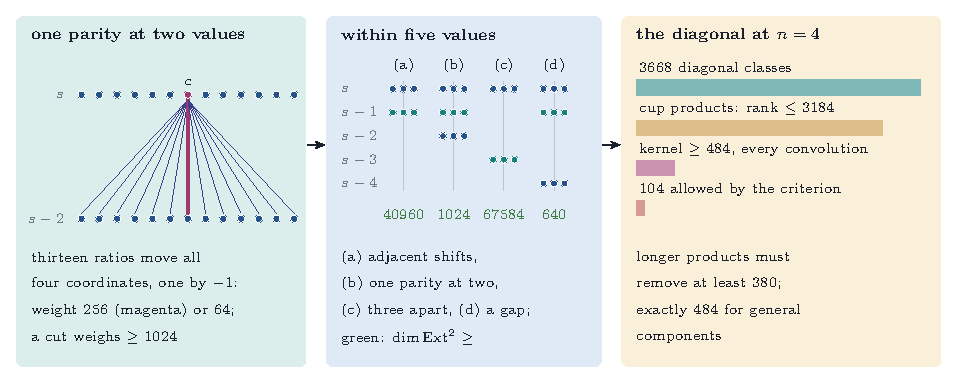
\includegraphics[width=\textwidth]{fig_efourspread}
\caption{The shift arrangements of the pieces $L_{\zeta}$ on $E_{0}^{8}$.
Left: one parity at two values two apart; a piece $c$ is joined to the
thirteen pieces whose ratio moves every coordinate, one by $-1$, and the
groups $\cH^{4}$ of the edges crossing between the values survive, weighing
at least $1024$ (\Cref{lem:efourspread}(ii), \Cref{lem:cayleycut}). Middle:
the four kinds of arrangement within five consecutive values, with the
result that excludes each and its bound on $\dim\Ext^{2}$. Right: the
diagonal at $n=4$; the cup products leave at least $484$ of the $3668$
classes, and the criterion allows $104$ (\Cref{prop:efourcupkernel}).}
\label{fig:efourspread}
\end{figure}

\begin{figure}[tbp]
\centering
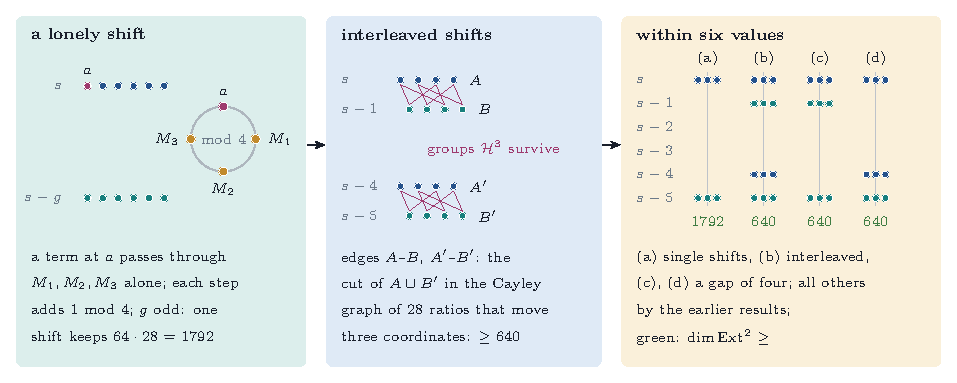
\includegraphics[width=\textwidth]{fig_efoursix}
\caption{The arrangements within six consecutive values on $E_{0}^{8}$.
Left: the parities at single shifts $s$ and $s-g$, $g$ odd and at least five;
a term on a diagonal class at a piece $a$ runs through $M_{1}$, $M_{2}$,
$M_{3}$ and no other piece, and since each step adds one to the shift modulo
$4$ the four nodes have distinct residues, so the multiples serve at most one
of the two shifts and the $1792$ diagonal classes at the other survive
(\Cref{lem:efourlonely}, \Cref{prop:efoursingle}). Middle: the interleaved
shifts; the groups $\cH^{3}$ between $A$ and $B$ and between $A'$ and $B'$
survive and form a cut of the Cayley graph of the $28$ ratios that move
three coordinates, of weight at least $640$ (\Cref{prop:efourpairs}).
Right: the four arrangements left within six values by the results for five
values, each with its bound on $\dim\Ext^{2}$ (\Cref{cor:efoursix}).}
\label{fig:efoursix}
\end{figure}

\begin{remark}[What the route gives]\label{rem:convolutionsopen}
At $n=3$ the route through convolutions of these pieces is decided. The
diagonal obstruction of \Cref{thm:esixdiagonal} leaves room only for the
fourfold products along one path, and the explicit convolution of
\Cref{prop:explicitconvolution} solves the Maurer--Cartan equation. The
obstruction that decides the route lies off the diagonal, in classes that no
product of any length can reach: those between pieces that differ in every coordinate and have
adjacent shifts (\Cref{lem:allthree}), and, at pieces whose shifts are not
adjacent to the shift of the paths, the classes of type $(1,1,0)$. No order
and no choice of shifts or twists avoids both, and
\Cref{thm:noconvolution} excludes every convolution of the $35$ pieces; in
the explicit convolution the first kind alone gives $2560$ classes against
the $57$ allowed. In each placement exactly two of the eight sign patterns
carry products, and the two are exchanged by a symmetry of the
construction.\footnote{The automorphism of $A$ that is $-1$ on the coordinate
$z_{n+1}$ and the identity on the others changes $\alpha$ into $-\alpha$,
fixes $\theta$ and permutes the $L_{\zeta}$, changing $\zeta_{1}$ into
$-\zeta_{1}$; composed with the shift $[1]$ it changes every $\sigma_{i}$
into $-\sigma_{i}$ and keeps everything else.} The member $E_{0}^{6}$ with
this Weil structure has trivial discriminant, where the Weil classes are
algebraic on every member by Markman's theorem \cite{Mar25a,Mar25b}, so a
convolution meeting the criterion here would have given a second proof of a
known case rather than a new one. At $n=4$ the classes between pieces that
differ in three coordinates and have adjacent shifts are again reached by
nothing, in every convolution, and when the pieces $L_{\zeta}$ occupy two
shifts, as in the explicit convolution, no term of $d_{E}$ leaves them, so
that $\dim\Ext^{2}(E,E)\ge40960$ against the $104$ allowed
(\Cref{thm:efourtwolevels}). With three consecutive shifts the
differential reaches these classes, but only through cup products into the
groups between the highest and the lowest shift, and at least $22528$ of
them survive (\Cref{thm:efourthreelevels}). The groups of spread three, and
those of spread two whose ratio moves every coordinate, one of them by $-1$,
are untouched as well, in every convolution
(\Cref{lem:efourspread}): the latter cross every cut between
two shift values of one parity, and weigh at least $1024$ there
(\Cref{thm:efourspreadtwo}); with one parity at a single shift, those of
spread three, or of spread one beside a gap, survive in their turn
(\Cref{thm:efourspreadthree}, \Cref{prop:efourgap}). Together they exclude
every convolution whose pieces $L_{\zeta}$ have their shifts within five
consecutive values (\Cref{cor:efourfive}). The two arrangements left within
six values fall as well: with each parity at a single shift, at any odd
distance, the diagonal classes at one of the two shifts can be reached only
through all three multiples, and the multiples serve at most one of them
(\Cref{lem:efourlonely}, \Cref{prop:efoursingle}); the interleaved shifts
leave the groups of \Cref{thm:efourtwolevels} on a cut
(\Cref{prop:efourpairs}). So every convolution whose shifts lie in six
consecutive values fails (\Cref{cor:efoursix}). For wider arrangements the
cup products still leave $484$ diagonal classes, so products of length at
least three would have to remove $380$ (\Cref{prop:efourcupkernel}), and
products of length three and four among the $L_{\zeta}$ pass every test of
\Cref{thm:esixdiagonal}. Whether some convolution of the $131$ pieces whose
shifts do not lie in six consecutive values, and whose parities do not each
sit at one shift, meets the criterion at $n=4$ is open. Markman's theorem
does not reach the eightfolds of Weil type, so such a convolution would give
a new case.
\Cref{fig:convolutions} shows the excess count and the
surviving path, and \Cref{fig:diagonalbudget} the budget of diagonal
classes.
\end{remark}
\subsubsection*{Markman's candidate in dimension eight}

Above $n=3$ there is one concrete candidate of this kind. Markman proposes
it in \cite[Section 12]{Mar25b} and notes that it remains to be checked
against the weakened criterion. Its Chern character is a finite computation
in the ring $\QQ[\Theta]/(\Theta^{5})$. We carry the computation out: it
places the candidate at a rational point of the secant plane of
\cite[Definition~14.4]{paperI} and reduces what has to be checked to a single
condition, which \Cref{thm:candidatefails} decides in the negative.

\begin{setupenv}[Markman's object]\label{setup:markman}
Let $(X,\Theta)$ be a principally polarised abelian fourfold, $d\ge3$ odd and
squarefree, $K=\QQ(\sqrt{-d})$ and $N=(d+9)/2$. Let $D_{i}$, $i\in\ZZ/N\ZZ$,
be $N$ translates of $\Theta$ in general position: any two, three or four of
them meet transversally, in a surface, a curve and $\Theta^{4}=24$ points,
and any five have empty intersection. Put $Z_{i}=D_{i}\cap D_{i+1}$,
$Z=\bigcup_{i}Z_{i}$, let $C_{i}=Z_{i}\cap Z_{i+1}=D_{i}\cap D_{i+1}\cap D_{i+2}$
be the curves along which consecutive components meet, and let
$\nu\colon\widetilde{Z}\to Z$ be the partial normalisation of $Z$ at
$m=(d+9)(2d-1)$ of its isolated points of self-intersection, the points of
$Z_{i}\cap Z_{j}$ for $i,j$ at cyclic distance at least three. Put
\[
  \cF=\bigl[\cO_{X}\longrightarrow\nu_{*}\cO_{\widetilde{Z}}\bigr]\otimes\cO_{X}(3\Theta),
\]
the complex placed in degrees $0$ and $1$.
\end{setupenv}

\begin{proposition}[Markman's candidate on the secant plane]
\label{prop:markman8}
In \Cref{setup:markman}, with $t=\Theta$ and $u_{t},v_{t}$ as in
\cite[(30)]{paperI} for $n=4$:
\begin{enumerate}[label=\textup{(\roman*)},nosep]
\item $\chi(\cO_{Z_{i}})=14$, $\chi(\cO_{C_{i}})=-36$, the isolated
  self-intersection points of $Z$ number $12N(N-5)=(d+9)(3d-3)$, and
  $\chi(\cO_{\widetilde Z})=110N-12N^{2}+2N(2d-1)=(d+9)(27-d)$;
\item $\ch(\nu_{*}\cO_{\widetilde Z})=N\Theta^{2}-2N\Theta^{3}
  +\chi(\cO_{\widetilde Z})\,[\mathrm{pt}]$;
\item $\ch(\cF)=u_{t}+3v_{t}$, that is
  \[
    \ch(\cF)=1+3\Theta-\tfrac{d}{2}\Theta^{2}-\tfrac{d}{2}\Theta^{3}
      +\tfrac{d^{2}}{24}\Theta^{4},
  \]
  the rational point $(a,b)=(1,3)$ of the secant plane $P_{\Theta}$; with
  the twist $\cO_{X}(\Theta)$ in place of $\cO_{X}(3\Theta)$ the degree two
  component would instead be $-\tfrac{d+8}{2}\Theta^{2}$, so the twist in
  \cite[Section 12]{Mar25b} must be read as $3\Theta$;
\item $\Nm_{K/\QQ}(3+\sqrt{-d})=d+9=2N$, with $N$ the number of divisors, and by
  \cite[Theorem~14.7]{paperI} the Bogomolov discriminant of $\cF$ is
  $\Delta(\cF)=(d+9)\Theta^{2}$;
\item the objects $\Phi(\cF\boxtimes\cF)$ and $\Phi(\cF\boxtimes\cF^{\vee})$
  on $X\times\widehat X$ have ranks
  $\int_{X}\ch(\cF)^{2}=8d(d-9)$ and
  $\int_{X}\ch(\cF)\ch(\cF^{\vee})=8d(d+9)$, up to sign, both nonzero for
  squarefree $d$; the same formula gives $-8q$ for the pair of secant sheaves
  of \cite[Section 11]{Mar25b} on a threefold, which is his rank $8q$ up to
  the shift.
\end{enumerate}
Consequently $\cF\boxtimes\cF$ satisfies conditions (1), (2b) and (2c) of
Markman's strategy \cite[Section 4]{Mar25b}: the transform has nonzero rank,
its normalised Chern character is invariant under the special Mumford--Tate
group by \cite[Corollary 9.2]{Mar25b}, and its Weil component is nonzero by
\cite[Proposition 10.2]{Mar25b}, the relevant coefficient being
$\Nm(c)$ with $c=\tfrac12(1+3/\sqrt{-d})\ne0$. What remains is condition
(2a) in its weakened form: for $E=\Phi(\cF\boxtimes\cF)$, the map
$\operatorname{ev}_{E}$ must kill every class in
$H^{1}(T)\oplus H^{0}(\bigwedge^{2}T)$ that preserves $\kappa(E)$ to first
order.
\end{proposition}

\begin{proof}
On a principally polarised abelian fourfold $\chi(\cO_{X}(k\Theta))=k^{4}$
and $\Theta^{4}=24$. The Koszul complex of $r$ transversal translates of
$\Theta$ gives $\ch$ of the structure sheaf of their intersection as
$(1-e^{-\Theta})^{r}$, so $\ch(\cO_{Z_{i}})=\Theta^{2}-\Theta^{3}+\tfrac{7}{12}\Theta^{4}$,
$\ch(\cO_{C_{i}})=\Theta^{3}-\tfrac32\Theta^{4}$ and $\ch$ of four divisors
is $\Theta^{4}$. Integrating gives $\chi(\cO_{Z_{i}})=14$,
$\chi(\cO_{C_{i}})=-36$ and $24$ points; the same numbers are the Koszul sums
$0-2\cdot1+16$, $0-3+48-81$ and $0-4+96-324+256$ of the values
$\chi(\cO_{X}(-k\Theta))=k^{4}$.

(i), (ii). At every point $Z$ is locally a union of coordinate subspaces of
$\CC^{4}$: along $C_{i}$ two surfaces $\{x_{1}=x_{2}=0\}\cup\{x_{2}=x_{3}=0\}$,
at a point of $C_{i}\cap C_{i+1}$ three of them, at an isolated point
$\{x_{1}=x_{2}=0\}\cup\{x_{3}=x_{4}=0\}$. The ideals of such an arrangement
are monomial and distribute over sums, so the Mayer--Vietoris complex
\[
  0\to\cO_{Z}\to\bigoplus_{i}\cO_{Z_{i}}\to\bigoplus_{i<j}\cO_{Z_{i}\cap Z_{j}}
  \to\bigoplus_{i<j<k}\cO_{Z_{i}\cap Z_{j}\cap Z_{k}}\to\cdots
\]
with scheme-theoretic intersections is exact. Pairs at cyclic distance one
meet in $C_{i}$, $N$ of them; pairs at distance at least two meet in the $24$
points of four divisors, $N(N-3)/2$ of them; the only triples with nonempty
intersection are the consecutive ones $Z_{i}\cap Z_{i+1}\cap Z_{i+2}=C_{i}\cap C_{i+1}$,
$24$ points each, $N$ of them; and no four components meet, since that would
involve at least five divisors. Hence
\[
  \ch(\cO_{Z})=N\ch(\cO_{Z_{i}})-N\ch(\cO_{C_{i}})-\tfrac{N(N-3)}{2}\Theta^{4}+N\Theta^{4},
\]
whose degree two part is $N\Theta^{2}$, degree three part
$-N\Theta^{3}-N\Theta^{3}=-2N\Theta^{3}$, and degree four part
$\chi(\cO_{Z})[\mathrm{pt}]$ with $\chi(\cO_{Z})=14N+36N-12N(N-3)+24N=110N-12N^{2}$.
The isolated singular points are those of pairs at distance at least three,
of which there are $N(N-5)/2$, giving $12N(N-5)=3(d+9)(d-1)$ points; the
pairs at distance two lie on the double curves and are not isolated. At an
isolated point the two branches meet transversally, and separating them
gives $0\to\cO_{Z}\to\nu_{*}\cO_{\widetilde Z}\to k(p)\to0$, so each of the
$m$ normalisations raises $\chi$ by one and leaves the lower degrees of
$\ch$ unchanged. With $N=(d+9)/2$,
$\chi(\cO_{\widetilde Z})=110N-12N^{2}+2N(2d-1)=(d+9)(55-3(d+9)+2d-1)=(d+9)(27-d)$.

(iii) $\ch(\cF)=e^{3\Theta}\bigl(1-\ch(\nu_{*}\cO_{\widetilde Z})\bigr)$. The
degree two part is $(\tfrac92-N)\Theta^{2}=-\tfrac d2\Theta^{2}$, which is
where $N=(d+9)/2$ enters; with the twist $k\Theta$ it would be
$(\tfrac{k^{2}}{2}-N)\Theta^{2}$, equal to $-\tfrac d2\Theta^{2}$ exactly for
$k^{2}=9$, and $k=-3$ is excluded by the degree three part. The degree three
part is $(\tfrac{27}{6}-3N+2N)\Theta^{3}=(\tfrac92-N)\Theta^{3}=-\tfrac d2\Theta^{3}$,
and the degree four part is
$(\tfrac{81}{24}-\tfrac{9N}{2}+6N-\tfrac{\chi(\cO_{\widetilde Z})}{24})\Theta^{4}
=\tfrac{81+36N-\chi(\cO_{\widetilde Z})}{24}\Theta^{4}=\tfrac{d^{2}}{24}\Theta^{4}$
by (i). Comparing with \cite[(30)]{paperI} at $n=4$,
$u_{t}=1-\tfrac d2t^{2}+\tfrac{d^{2}}{24}t^{4}$ and $v_{t}=t-\tfrac d6t^{3}$,
gives $\ch(\cF)=u_{t}+3v_{t}$.

(iv) This follows from $\Nm(3+\sqrt{-d})=9+d$ and \cite[(31)]{paperI} with
$(a,b)=(1,3)$.

(v) Orlov's equivalence is $\Phi=(\id\times\Phi_{\cP})^{-1}\circ\mu^{*}$ with
$\mu(x,y)=(x+y,y)$, so the restriction of $\Phi(\cF_{1}\boxtimes\cF_{2})$ to
$\{x\}\times\widehat X$ is the Fourier--Mukai transform of
$\tau_{x}^{*}\cF_{1}\otimes\cF_{2}$, whose derived fibre at $L\in\widehat X$
is $R\Gamma(X,\tau_{x}^{*}\cF_{1}\otimes\cF_{2}\otimes L^{\pm1})$; the rank
of a perfect complex is the Euler characteristic of its derived fibre, and
$\chi(\tau_{x}^{*}\cF_{1}\otimes\cF_{2}\otimes L)=\int_{X}\ch(\cF_{1})\ch(\cF_{2})$
by Riemann--Roch, translations and $L\in\Pic^{0}$ acting trivially on
cohomology. With $\ch(\cF^{\vee})=u_{t}-3v_{t}$, the involution $\tau$
changing the sign of the odd degrees, $\int u_{t}^{2}=8d^{2}$,
$\int u_{t}v_{t}=0$ and $\int v_{t}^{2}=-8d$ give the two values. On a
threefold $\int(u_{t}+v_{t})^{2}=2\int u_{t}v_{t}=-8q$.

For the final assertion, condition (2b) is the
$\mathrm{Spin}(V_{\QQ})_{B}$-invariance of $\kappa(E)$, which
\cite[Corollary 9.2]{Mar25b} derives from $\ch(\cF)\in B$ and the
nonvanishing of the rank. Condition (2c) is
\cite[Proposition 10.2]{Mar25b}, which for $K$ imaginary quadratic reduces
to the nonvanishing of the component of $\ch(\cF)\otimes\ch(\cF)$ in
$\ell_{W}\otimes\ell_{\bbar W}$, and writing $\ch(\cF)=c\,\ell_{W}+\bbar c\,\ell_{\bbar W}$
with $\ell_{W}=e^{\sqrt{-d}\Theta}$ gives that coefficient as $c\bbar c$.
\end{proof}

\begin{remark}[The remaining condition]\label{rem:onecondition}
\Cref{prop:markman8} does not verify Markman's candidate. It verifies every
statement about the candidate that concerns classes, and it shows that the
one remaining statement concerns the object. For
$E=\Phi(\cF\boxtimes\cF)$ on the eightfold $X\times\widehat X$ of Weil type,
with $\kappa(E)=\ch(E)e^{-c_{1}(E)/\operatorname{rk}E}$, that statement reads:
every $x\in H^{1}(T)\oplus H^{0}(\bigwedge^{2}T)$ with
$x\lrcorner\,\kappa(E)=0$ satisfies $\operatorname{ev}_{E}(x)=0$ in
$\Ext^{2}(E,E)$. The $H^{2}(\cO)$ summand imposes nothing, because
$\operatorname{rk}E\ne0$ makes $z\cdot\kappa(E)\ne0$ for $z\ne0$. By
\cite[Theorem~9.20]{paperI} the condition fails as soon as $E$ has a rank one
direct summand whose class is not a multiple of the polarisation, so the
first question about $E$ is whether it is indecomposable. Markman's object
at $n=3$ is reflexive of rank $8q$ away from a divisor, and he proves the
condition by descending to a quotient on which $\sigma_{E}$ is injective on
an invariant subspace \cite[Proposition 11.5]{Mar25b}. Whether the same can
be done for $\Phi(\cF\boxtimes\cF)$ is a question about the Ext groups of one
object on one eightfold, not about any Hodge class. \Cref{thm:factor} below
moves the question from the eightfold to the fourfold and from $E$ to $\cF$
itself: the condition is equivalent to the single identity
\eqref{eq:heisenberg} in $\Ext^{2}(\cF,\cF\otimes\Omega^{2}_{X})$, the other
half of it holding by construction. \Cref{thm:candidatefails} shows that the
identity fails, so the answer is negative.
\end{remark}

\subsubsection*{Reduction to the fourfold}

The condition of \Cref{rem:onecondition} concerns an object on an eightfold.
It is equivalent to a condition on the factor $\cF$ on the fourfold, and
there it splits into two conditions, one of which holds for Markman's object
because the object is constructed uniformly over the moduli of principally
polarised fourfolds. The reduction is not special to that object. It works
for every secant object on every abelian $n$-fold with $n\ge3$, and its
ingredients are three computations in the Hodge algebra of a single abelian
variety, which we carry out by hand. We first fix
conventions.

\begin{setupenv}[The weakened criterion for one object]\label{setup:criterion}
Let $Y$ be an abelian variety and $F$ a nonzero perfect complex on $Y$. Write
$HT^{2}(Y)=H^{0,2}(Y)\oplus H^{1}(T_{Y})\oplus H^{0}(\bigwedge^{2}T_{Y})$ as
in \eqref{eq:HT2}, with $x=(z,v,\pi)$ acting on $H^{*}(Y,\CC)$ by
$x\lrcorner$, and likewise $HT^{1}(Y)=H^{0,1}(Y)\oplus H^{0}(T_{Y})$, with
$(z,\theta)$ acting by $z\wedge$ and by the interior product $\theta\lrcorner$.
Normalise the Atiyah class $\mathrm{At}(F)\in\Ext^{1}(F,F\otimes\Omega^{1}_{Y})$
so that $\ch(F)=\operatorname{tr}\exp\mathrm{At}(F)$; for a line bundle $L$
it is then $c_{1}(L)$, as in \eqref{eq:obdef}.%
\footnote{This is the convention of \cite{Tod09} and of
\cite[footnote 14]{Mar25a}. Buchweitz and Flenner use the opposite sign,
which replaces $\mathrm{At}(F)$ by $-\mathrm{At}(F)$; this leaves
$\mathrm{At}(F)^{2}$ unchanged and changes only the sign of the middle term
of $\operatorname{ev}_{F}$, which does not affect the vanishing statements
below.}
The evaluation map of \cite[Theorem~9.19]{paperI} is, under HKR,
\begin{equation}\label{eq:evgeneral}
  \operatorname{ev}_{F}(z,v,\pi)=z\cdot\id_{F}+v\lrcorner\,\mathrm{At}(F)
  +\tfrac12\,\pi\lrcorner\,\mathrm{At}(F)^{2}\;\in\;\Ext^{2}(F,F),
\end{equation}
the contraction of the polyvector with the exponential Atiyah class
\cite[Theorem A]{Hua21}, \cite{BF08}; its restriction to $H^{1}(T_{Y})$ is the
obstruction map, whose kernel is the space of first order deformations of $Y$
to which $F$ extends \cite{Tod09}, \cite[Section 8.3]{Mar25a}. Put
\[
  \Ann_{HT^{2}}(\ch F)=\bigl\{x\in HT^{2}(Y):x\lrcorner\,\ch(F)=0\bigr\},
\]
the Hochschild classes preserving $\ch(F)$ to first order. We say that $F$
\emph{satisfies the weakened criterion} if $\operatorname{ev}_{F}$ vanishes on
$\Ann_{HT^{2}}(\ch F)$. By the commutative square
$\sigma_{F}\circ\operatorname{ev}_{F}=(\,\cdot\,)\lrcorner\,\ch(F)$ of
\cite[Proposition 6.2.1 and Corollary 6.3.2]{BF08}, in the form quoted in
\cite[Lemma 11.3]{Mar25b},
\[
  \operatorname{ev}_{F}\bigl(\Ann_{HT^{2}}(\ch F)\bigr)
  =\ker\sigma_{F}\cap\image\operatorname{ev}_{F},
\]
so the weakened criterion is exactly the hypothesis of
\cite[Question 11.4]{Mar25b}, that the restriction of $\sigma_{F}$ to the
image of $\operatorname{ev}_{F}$ is injective. For a split object this is
\Cref{prop:evaluation}(ii).
\end{setupenv}

\begin{lemma}[The $B$-field transform]\label{lem:bfield}
Let $B\in H^{1,1}(Y)$. For $x=(z,v,\pi)\in HT^{2}(Y)$ put
\begin{equation}\label{eq:bfield}
  e^{B}x=\bigl(z+v\lrcorner\,B+\tfrac12\,\pi\lrcorner\,B^{2},\;
  v+\pi\lrcorner\,B,\;\pi\bigr),
\end{equation}
where $\pi\lrcorner\,B\in\Hom(H^{1,0},H^{0,1})=H^{1}(T_{Y})$ is the contraction
of one slot of $\pi$ with $B$: for $\pi=\partial_{a}\wedge\partial_{b}$ it sends
$p_{b}$ to $\partial_{a}\lrcorner\,B$, $p_{a}$ to $-\partial_{b}\lrcorner\,B$
and the other basis vectors to zero. Then $e^{B}$ is a linear automorphism of
$HT^{2}(Y)$ with inverse $e^{-B}$, and:
\begin{enumerate}[label=\textup{(\roman*)},nosep]
\item $x\lrcorner\,(w\,e^{B})=\bigl((e^{B}x)\lrcorner\,w\bigr)\,e^{B}$ for
  every even class $w\in H^{\mathrm{ev}}(Y,\CC)$;
\item for a line bundle $L$ with $c_{1}(L)=B$,
  $\operatorname{ev}_{F\otimes L}(x)=\operatorname{ev}_{F}(e^{B}x)$ and
  $\Ann_{HT^{2}}(\ch(F\otimes L))=e^{-B}\Ann_{HT^{2}}(\ch F)$; hence $F$
  satisfies the weakened criterion if and only if $F\otimes L$ does.
\end{enumerate}
The computation in (ii) is formal: it uses only that the twisted object has
Atiyah class $\mathrm{At}(F)+B\cdot\id_{F}$ and Chern character
$\ch(F)e^{B}$. It therefore applies verbatim to the twisted sheaves of
\cite[Section 2]{Mar25b}, with $B$ rational. In particular, for $F$ of
nonzero rank $r$, the criterion for the twisted object $F\otimes L^{-1}$ with class
$\kappa(F)=\ch(F)e^{-c_{1}(F)/r}$ is the same condition as the criterion for
$F$ with class $\ch(F)$.
\end{lemma}

\begin{proof}
The computation takes place in a graded algebra on which the interior
products $\iota_{a}=\partial_{a}\lrcorner$ act as odd derivations. It uses
only that $w$ is even; that $B$ is even and central with
$\iota_{a}\iota_{b}B=0$, which holds for $B$ of type $(1,1)$ and
$\partial_{a},\partial_{b}$ of type $(1,0)$; and that the odd scalar classes
$\iota_{a}B$ anticommute with every odd element. In $H^{*}(Y,\CC)$ these
properties are clear. They also hold in
$\bigoplus_{p,q}\Ext^{p}(F,F\otimes\Omega^{q}_{Y})=\Ext^{*}(F,F)\otimes
\bigwedge^{*}H^{1,0}$, on which the polyvectors act through the second factor
by odd derivations, because the classes coming from $H^{*}(Y,\CC)$ are graded
central in the Yoneda algebra. First, $\iota_{a}(B^{k})=k(\iota_{a}B)B^{k-1}$,
since $\iota_{a}B$ is odd and $B$ is even, so
$\iota_{a}e^{B}=(\iota_{a}B)e^{B}$. For $w$ even this gives
$v\lrcorner\,(we^{B})=(v\lrcorner\,w)e^{B}+w\sum_{a}v(p_{a})(\iota_{a}B)e^{B}
=\bigl(v\lrcorner\,w+(v\lrcorner\,B)w\bigr)e^{B}$, and
$z(we^{B})=(zw)e^{B}$. For the bivector, with $\pi\lrcorner=\iota_{a}\iota_{b}$,
\[
  \iota_{b}(we^{B})=(\iota_{b}w)e^{B}+w(\iota_{b}B)e^{B},
\]
and applying $\iota_{a}$, using that $\iota_{b}w$ and $\iota_{b}B$ are odd,
\[
  \iota_{a}\iota_{b}(we^{B})
  =\bigl[\iota_{a}\iota_{b}w
   +(\iota_{a}B)\iota_{b}w-(\iota_{b}B)\iota_{a}w
   +w\bigl((\iota_{a}\iota_{b}B)-(\iota_{b}B)(\iota_{a}B)\bigr)\bigr]e^{B}.
\]
The middle two terms are $(\pi\lrcorner\,B)\lrcorner\,w$ for the element
$\pi\lrcorner\,B$ of $\Hom(H^{1,0},H^{0,1})$ displayed in the statement, acting
as a derivation, and the last bracket is
$\tfrac12\iota_{a}\iota_{b}(B^{2})=\iota_{a}\bigl((\iota_{b}B)B\bigr)$.
Summing the three actions gives (i). Applying (i) with $B$ replaced by $-B$
and then by $B$, and using
$(\pi\lrcorner\,B)\lrcorner\,B=2(\iota_{a}B)(\iota_{b}B)=\pi\lrcorner\,B^{2}$
when $\iota_{a}\iota_{b}B=0$, shows $e^{-B}e^{B}=\id$.

(ii) The Atiyah class of $F\otimes L$ is $\mathrm{At}(F)+B\cdot\id_{F}$,
the Atiyah class being additive on tensor products \cite[Section 3]{BF03},
and the two summands commute, so
$\exp\mathrm{At}(F\otimes L)=\exp\mathrm{At}(F)\cdot e^{B}$. By (i) in the
algebra $\Ext^{*}(F,F)\otimes\bigwedge^{*}H^{1,0}$, with $w=\exp\mathrm{At}(F)$,
\[
  x\lrcorner\,\exp\mathrm{At}(F\otimes L)
  =\bigl((e^{B}x)\lrcorner\,\exp\mathrm{At}(F)\bigr)e^{B},
\]
and the right hand side has the same component in
$\Ext^{2}(F,F)\otimes\bigwedge^{0}$ as $(e^{B}x)\lrcorner\,\exp\mathrm{At}(F)$,
because $e^{B}-1=B+\tfrac12B^{2}+\cdots$ raises the exterior degree. This is
$\operatorname{ev}_{F\otimes L}(x)=\operatorname{ev}_{F}(e^{B}x)$. By (i) in
$H^{*}(Y,\CC)$ with $w=\ch(F)$, $x\lrcorner\,\ch(F\otimes L)=0$ if and only
if $(e^{B}x)\lrcorner\,\ch(F)=0$, which is the statement on the annihilators.
Hence $\operatorname{ev}_{F\otimes L}(\Ann_{HT^{2}}(\ch(F\otimes L)))
=\operatorname{ev}_{F}(\Ann_{HT^{2}}(\ch F))$.
\end{proof}

\begin{theorem}[Reduction to the factor]\label{thm:factor}
Let $(X,t)$ be a polarised abelian variety of dimension $n\ge3$, let $d\ge1$,
and let $F$ be a perfect complex on $X$ with
$\ch(F)=a\,u_{t}+b\,v_{t}$ for some $(a,b)\in\QQ^{2}\setminus\{0\}$, in the
notation of \cite[(30)]{paperI}. Then:
\begin{enumerate}[label=\textup{(\roman*)},nosep]
\item No nonzero class in $HT^{1}(X)$ preserves $\ch(F)$: the map
  $HT^{1}(X)\to H^{*}(X,\CC)$, $y\mapsto y\lrcorner\,\ch(F)$, is injective. Its
  two lowest components form the matrix
  $\bigl(\begin{smallmatrix}a&b\\ b&-ad\end{smallmatrix}\bigr)$ of
  determinant $-(a^{2}d+b^{2})=-\Nm_{K/\QQ}(b+a\sqrt{-d})\ne0$.
\item The classes in $HT^{2}(X)$ preserving $\ch(F)$ to first order are
  \begin{equation}\label{eq:secantkernel}
    \Ann_{HT^{2}}(\ch F)
    =\bigl\{(0,v,0):v\lrcorner\,t=0\bigr\}\;\oplus\;
     \bigl\{(\tfrac d2\,\pi\lrcorner\,t^{2},\,0,\,\pi):
       \pi\in H^{0}(\textstyle\bigwedge^{2}T_{X})\bigr\},
  \end{equation}
  the polarised first order deformations of $(X,t)$, of dimension $n(n+1)/2$,
  and the Poisson directions each compensated by a class in $H^{0,2}$, of
  dimension $n(n-1)/2$; the total is $n^{2}=\dim\cD_{n,n}$, and the space
  does not depend on $(a,b)$.
\item $F$ satisfies the weakened criterion if and only if
  \begin{enumerate}[label=\textup{(\alph*)},nosep]
  \item $v\lrcorner\,\mathrm{At}(F)=0$ in $\Ext^{2}(F,F)$ for every
    $v\in H^{1}(T_{X})$ with $v\lrcorner\,t=0$, that is, $F$ extends to first
    order along every polarised deformation of $(X,t)$; and
  \item $\mathrm{At}(F)^{2}=-d\,t^{2}\cdot\id_{F}$ in
    $\Ext^{2}(F,F\otimes\Omega^{2}_{X})$.
  \end{enumerate}
  The trace of (b) is automatic: $\operatorname{tr}\mathrm{At}(F)^{2}
  =2\ch_{2}(F)=-ad\,t^{2}=\operatorname{tr}(-d\,t^{2}\cdot\id_{F})$, so (b)
  is the vanishing of the trace free part of the square of the Atiyah class.
\item Let $F_{1},F_{2}$ be two such complexes, $G=F_{1}\boxtimes F_{2}$ on
  $X\times X$ and $E=\Phi(G)$ on $X\times\widehat X$, with $\Phi$ Orlov's
  equivalence as in \Cref{prop:markman8}(v). Then
  $\Ann_{HT^{2}}(\ch G)=\Ann_{HT^{2}}(\ch F_{1})\otimes1\oplus
  1\otimes\Ann_{HT^{2}}(\ch F_{2})$, of dimension $2n^{2}$, and
  \[
    E\ \text{satisfies the weakened criterion}
    \iff G\ \text{does}
    \iff F_{1}\ \text{and}\ F_{2}\ \text{do}.
  \]
\end{enumerate}
\end{theorem}

\begin{proof}
Choose a basis $p_{1},\dots,p_{n}$ of $H^{1,0}(X)$ and a basis
$q_{1},\dots,q_{n}$ of $H^{0,1}(X)$ with $t=\sum_{a}p_{a}\wedge q_{a}$, which
is possible because $t$ is a positive class of type $(1,1)$; let
$\partial_{a}$ be the dual basis of $T$, so that $\iota_{a}p_{b}=\delta_{ab}$
and $\iota_{a}q_{b}=0$. Write $\ch(F)=\sum_{k}c_{k}t^{k}$ with
$c_{k}\,k!=a(-d)^{k/2}$ for $k$ even and $c_{k}\,k!=b(-d)^{(k-1)/2}$ for $k$
odd, so that
\begin{equation}\label{eq:crecursion}
  c_{k+1}\,(k+1)!=-d\,c_{k-1}\,(k-1)!\qquad(k\ge1).
\end{equation}
Two facts about the Hodge algebra are used throughout: for $v\in H^{1}(T)$
acting as a derivation, $v\lrcorner\,t^{k}=k\,(v\lrcorner\,t)\,t^{k-1}$; and
for a bivector $\pi$ of type $(2,0)$ in the tangent directions,
$\pi\lrcorner\,t=0$ because $t$ has a single $(1,0)$ slot in each term, so
$\pi\lrcorner\,t^{k}=\binom{k}{2}(\pi\lrcorner\,t^{2})\,t^{k-2}$ by the footnote
to \eqref{eq:HT2}. Finally, multiplication by $t$ is injective on $H^{0,1}$
when $n\ge2$ and on $H^{0,2}$ when $n\ge3$: $q_{a}\wedge t$ contains the
monomial $p_{c}q_{c}q_{a}$ for any $c\ne a$, and $q_{a}q_{b}\wedge t$ contains
$p_{c}q_{c}q_{a}q_{b}$ for any $c\notin\{a,b\}$, and distinct monomials are
independent.

(i) For $y=(z,\theta)$ the class $y\lrcorner\,\ch(F)$ has components of type
$(k-1,k)$ equal to $c_{k-1}z\,t^{k-1}+c_{k}\,\theta\lrcorner\,t^{k}
=\bigl(c_{k-1}z+k\,c_{k}\,(\theta\lrcorner\,t)\bigr)t^{k-1}$. For $k=1$ this
is $az+b\,(\theta\lrcorner\,t)$ and for $k=2$ it is
$\bigl(bz-ad\,(\theta\lrcorner\,t)\bigr)t$, by \eqref{eq:crecursion}. Both
$z$ and $\theta\lrcorner\,t=\sum_{a}\theta^{a}q_{a}$ lie in $H^{0,1}$, on which
$t$ acts injectively, so $y\lrcorner\,\ch(F)=0$ forces
$(z,\theta\lrcorner\,t)$ into the kernel of the displayed matrix, whose
determinant is $-a^{2}d-b^{2}<0$. Hence $z=0$ and $\theta\lrcorner\,t=0$, and
the latter gives $\theta=0$ because $t$ is nondegenerate.

(ii) For $x=(z,v,\pi)$ the component of $x\lrcorner\,\ch(F)$ of type
$(k-1,k+1)$ is
\[
  c_{k-1}z\,t^{k-1}+c_{k}\,v\lrcorner\,t^{k}+c_{k+1}\,\pi\lrcorner\,t^{k+1}
  =\Bigl(c_{k-1}z+k\,c_{k}\,W+\tbinom{k+1}{2}c_{k+1}\,P\Bigr)t^{k-1},
\]
with $W=v\lrcorner\,t$ and $P=\pi\lrcorner\,t^{2}$, both in $H^{0,2}$. By
\eqref{eq:crecursion}, $\binom{k+1}{2}c_{k+1}=-\tfrac d2c_{k-1}$, so the bracket
is $c_{k-1}Z+k\,c_{k}W$ with $Z=z-\tfrac d2P$. For $k=1$ and $k=2$ this gives
$aZ+bW$ and $(bZ-adW)\,t$, and $t$ is injective on $H^{0,2}$ because $n\ge3$;
the same determinant forces $Z=W=0$. Conversely $Z=W=0$ kills every
component. So $\Ann_{HT^{2}}(\ch F)$ is the set of $(z,v,\pi)$ with
$v\lrcorner\,t=0$ and $z=\tfrac d2\,\pi\lrcorner\,t^{2}$, which is
\eqref{eq:secantkernel}; the two summands are independent because the first
has $\pi=0$ and the second is the graph of a linear map from the $\pi$
component. A $v\in\Hom(H^{1,0},H^{0,1})$ has $v\lrcorner\,t=\sum_{a}v(p_{a})\wedge q_{a}$,
which vanishes exactly when the matrix of $v$ is symmetric; this is the
tangent space of the polarised deformations, of dimension $n(n+1)/2$, as in
\Cref{prop:splitobstruction}(i). The bivectors contribute
$\dim\bigwedge^{2}T=n(n-1)/2$. Nothing in the description involves $(a,b)$.

(iii) By (ii) and \eqref{eq:evgeneral}, $\operatorname{ev}_{F}$ vanishes on
$\Ann_{HT^{2}}(\ch F)$ if and only if it vanishes on both summands. On the
first it is $v\mapsto v\lrcorner\,\mathrm{At}(F)$, which is (a). On the
second it is
\[
  \tfrac d2(\pi\lrcorner\,t^{2})\cdot\id_{F}+\tfrac12\,\pi\lrcorner\,\mathrm{At}(F)^{2}
  =\tfrac12\,\pi\lrcorner\bigl(\mathrm{At}(F)^{2}+d\,t^{2}\cdot\id_{F}\bigr),
\]
since $\pi\lrcorner\,(t^{2}\cdot\id_{F})=(\pi\lrcorner\,t^{2})\cdot\id_{F}$.
Now $\Omega^{2}_{X}=\cO_{X}\otimes\bigwedge^{2}H^{1,0}$, so
$\Ext^{2}(F,F\otimes\Omega^{2}_{X})=\Ext^{2}(F,F)\otimes\bigwedge^{2}H^{1,0}$,
and the contractions with all $\pi\in\bigwedge^{2}(H^{1,0})^{\vee}$ vanish on
an element of this space if and only if the element is zero, the pairing
being perfect. This is (b). For the trace, $\ch(F)=\operatorname{tr}\exp\mathrm{At}(F)$
gives $\ch_{2}(F)=\tfrac12\operatorname{tr}\mathrm{At}(F)^{2}$, and
$\ch_{2}(F)=c_{2}t^{2}=-\tfrac{ad}{2}t^{2}$, while
$\operatorname{tr}(\id_{F})=\rk F=c_{0}=a$.

(iv) The Hochschild cohomology of a product is the tensor product,
$HT^{2}(X\times X)=HT^{2}\otimes HT^{0}\oplus HT^{1}\otimes HT^{1}\oplus
HT^{0}\otimes HT^{2}$, the Atiyah class of $G$ is
$\mathrm{At}(F_{1})\boxtimes1+1\boxtimes\mathrm{At}(F_{2})$ \cite[Proposition 3.14]{BF03},
\cite[(8.4.1)]{Mar25a}, so $\exp\mathrm{At}(G)=\exp\mathrm{At}(F_{1})\boxtimes
\exp\mathrm{At}(F_{2})$, and $\Ext^{2}(G,G)$ is the corresponding K\"unneth
sum of $\Ext^{i}(F_{1},F_{1})\otimes\Ext^{j}(F_{2},F_{2})$. A polyvector on a
factor contracts only the forms of that factor, so for $x_{1}\in HT^{i}(X)$
and $x_{2}\in HT^{j}(X)$ with $i+j=2$,
\[
  (x_{1}\otimes x_{2})\lrcorner\,\ch(G)=\pm(x_{1}\lrcorner\,\ch F_{1})\otimes
  (x_{2}\lrcorner\,\ch F_{2}),\qquad
  \operatorname{ev}_{G}(x_{1}\otimes x_{2})=\pm\operatorname{ev}_{F_{1}}(x_{1})
  \otimes\operatorname{ev}_{F_{2}}(x_{2}),
\]
with $\operatorname{ev}(1)=\id$ on $HT^{0}$ and Koszul signs that play no
role; this is the decomposition \cite[(8.4.2), (8.4.3)]{Mar25a}. Let
$x=x_{20}+x_{11}+x_{02}$ be a class in $\Ann_{HT^{2}}(\ch G)$ according to the
three summands. Since $\ch(F_{i})$ is even, $x_{11}\lrcorner\,\ch(G)$ lies in
$H^{\mathrm{odd}}\otimes H^{\mathrm{odd}}$ while the other two terms lie in
$H^{\mathrm{ev}}\otimes H^{\mathrm{ev}}$, so $x_{11}\lrcorner\,\ch(G)=0$
separately; and $x_{11}\lrcorner\,\ch(G)$ is the image of $x_{11}$ under the
tensor product of the two maps of (i), which is injective, so $x_{11}=0$. For
the even part write $x_{20}=x_{1}\otimes1$ and $x_{02}=1\otimes x_{2}$; then
$(x_{1}\lrcorner\,\ch F_{1})\otimes\ch(F_{2})+\ch(F_{1})\otimes(x_{2}\lrcorner\,\ch F_{2})=0$.
Applying a linear form on the second factor taking the value $1$ on
$\ch(F_{2})$ shows $x_{1}\lrcorner\,\ch(F_{1})=\lambda\,\ch(F_{1})$ for a
scalar $\lambda$, and then $x_{2}\lrcorner\,\ch(F_{2})=-\lambda\,\ch(F_{2})$.
But every component of $x_{1}\lrcorner\,\ch(F_{1})$ has Hodge type $(p,p+2)$
while $\ch(F_{1})\ne0$ has type $(p,p)$; so $\lambda=0$ and
$x_{i}\in\Ann_{HT^{2}}(\ch F_{i})$. This proves the description of
$\Ann_{HT^{2}}(\ch G)$ and its dimension $2n^{2}$ by (ii). On it
$\operatorname{ev}_{G}(x_{1}\otimes1+1\otimes x_{2})=\pm\operatorname{ev}_{F_{1}}(x_{1})
\otimes\id_{F_{2}}\pm\id_{F_{1}}\otimes\operatorname{ev}_{F_{2}}(x_{2})$, whose
two terms lie in different K\"unneth summands and vanish exactly when
$\operatorname{ev}_{F_{i}}(x_{i})=0$, as $\id_{F_{i}}\ne0$. So $G$ satisfies
the criterion if and only if $F_{1}$ and $F_{2}$ do.

For the transport under $\Phi$ we use the commutative diagram of
\cite[Lemma 8.3.10]{Mar25a}: an equivalence $\Phi\colon D^{b}(A)\to D^{b}(B)$
of derived categories of abelian varieties induces isomorphisms
$\Phi^{HT}\colon HT^{2}(A)\to HT^{2}(B)$ and $\Phi^{H}\colon H^{*}(A,\CC)\to
H^{*}(B,\CC)$ with $\Phi^{H}(x\lrcorner\,\ch G)=\Phi^{HT}(x)\lrcorner\,\ch\Phi(G)$
\cite{CRV12}, and $\Phi\circ\operatorname{ev}_{G}=\operatorname{ev}_{\Phi(G)}\circ\Phi^{HT}$
on $\Hom(G,G[2])\to\Hom(\Phi G,\Phi G[2])$ \cite[Theorem A]{Hua21}; on abelian
varieties the Todd class is trivial, so there is no Duflo correction
\cite[Remark 8.3.11]{Mar25a}. The first square gives
$\Phi^{HT}\bigl(\Ann_{HT^{2}}(\ch G)\bigr)=\Ann_{HT^{2}}(\ch E)$ and the second
$\operatorname{ev}_{E}\bigl(\Ann_{HT^{2}}(\ch E)\bigr)
=\Phi\bigl(\operatorname{ev}_{G}(\Ann_{HT^{2}}(\ch G))\bigr)$, with $\Phi$ an
isomorphism on $\Ext^{2}$. So $E$ satisfies the criterion if and only if $G$
does.
\end{proof}

\Cref{fig:factor} draws the K\"unneth stack and the two conditions at
$n=4$.

\begin{figure}[tbp]
\centering
  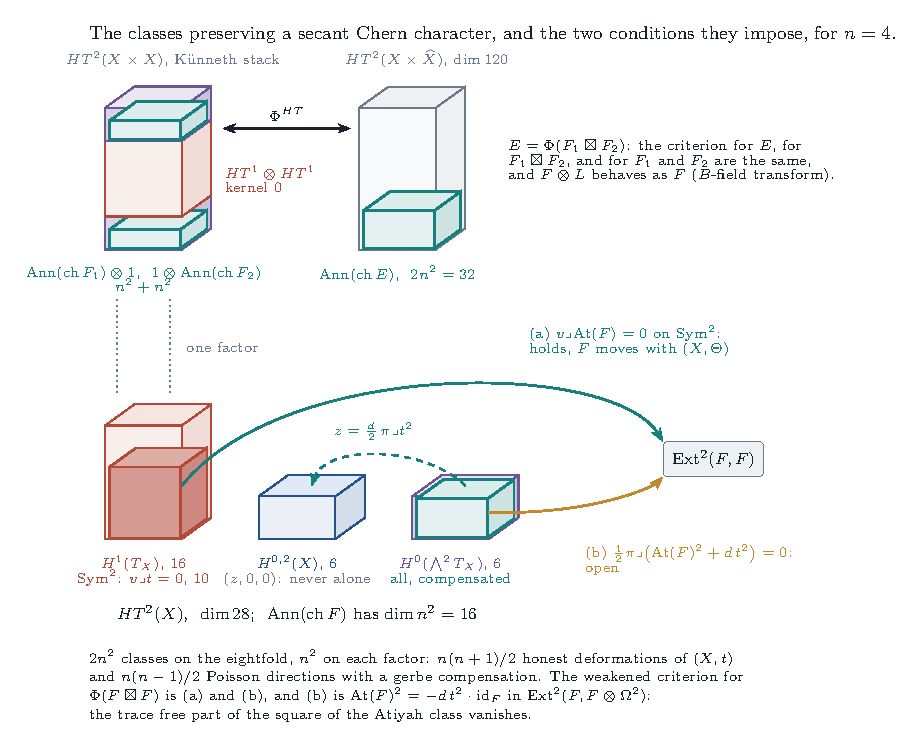
\includegraphics[width=\textwidth]{fig_factor}
\caption{\Cref{thm:factor} for $n=4$. Top: the K\"unneth stack of
$HT^{2}(X\times X)$, whose middle summand $HT^{1}\otimes HT^{1}$ meets the
kernel in zero by (i), so that the classes preserving $\ch(F_{1}\boxtimes F_{2})$
are two copies of the kernel on one factor; across Orlov's isomorphism,
$HT^{2}$ of the eightfold with the $2n^{2}$ classes preserving $\ch(E)$.
Bottom: $HT^{2}(X)$ as three slabs with heights proportional to their
dimensions, and inside them the $n^{2}$ classes of \eqref{eq:secantkernel}:
the polarised deformations in front of $H^{1}(T_{X})$, and the whole of
$H^{0}(\bigwedge^{2}T_{X})$, each bivector tilted into $H^{0,2}$ by its
compensation $\tfrac d2\,\pi\lrcorner t^{2}$; nothing in $H^{0,2}$ alone
preserves $\ch(F)$. On the right, the two conditions that the evaluation map
imposes on the two parts, (a) closed by the construction of $\cF$ and (b)
the identity \eqref{eq:heisenberg}.}
\label{fig:factor}
\end{figure}

\begin{corollary}[The remaining condition on the fourfold]\label{cor:markmancondition}
In \Cref{setup:markman} let $E=\Phi(\cF\boxtimes\cF)$. Then $E$ satisfies the
weakened criterion of \cite[Question 11.4]{Mar25b} if and only if
\begin{equation}\label{eq:heisenberg}
  \mathrm{At}(\cF)^{2}=-d\,\Theta^{2}\cdot\id_{\cF}
  \qquad\text{in }\Ext^{2}(\cF,\cF\otimes\Omega^{2}_{X}).
\end{equation}
Equivalently, writing $\mathrm{At}(\cF)=\sum_{a}A_{a}\otimes p_{a}$ with
$A_{a}\in\Ext^{1}(\cF,\cF)$ in a basis $p_{a}$ of $H^{1,0}(X)$, and
$\Theta=\sum_{a}p_{a}\wedge q_{a}$ with $q_{a}\in H^{0,1}(X)$, all the
commutators $A_{a}A_{b}-A_{b}A_{a}\in\Ext^{2}(\cF,\cF)$ are the scalars
$\pm2d\,(q_{a}\wedge q_{b})\cdot\id_{\cF}$ prescribed by $\Theta^{2}$, the
sign being fixed by the Koszul rule.
\end{corollary}

\begin{proof}
By \Cref{prop:markman8}(iii), $\ch(\cF)=u_{\Theta}+3v_{\Theta}$, so
\Cref{thm:factor} applies with $n=4$, $(a,b)=(1,3)$ and $F_{1}=F_{2}=\cF$, and
$E$ satisfies the criterion if and only if $\cF$ satisfies (a) and (b). It
remains to show that (a) holds. The data of \Cref{setup:markman} are a
principally polarised fourfold $(X,\Theta)$ and $N$ points $x_{i}\in X$ with
$D_{i}=\tau_{x_{i}}^{*}\Theta$. The conditions imposed on the $D_{i}$, that
the intersections of two, three and four of them be smooth of the expected
codimension and that five of them be disjoint, are open in the parameter
space of such data over the local universal deformation $S$ of $(X,\Theta)$,
by the openness of smoothness for a proper flat family and the properness of
the projection. The isolated points of $Z$, being transversal intersections
of four divisors, form a finite \'etale cover of the open set where the
conditions hold, so the $m$ points to be normalised can be followed locally;
the partial normalisation separates two smooth branches at each of them and
commutes with base change. The construction therefore produces a perfect
complex $\cF_{S}$ on the universal family over a neighbourhood of the base
point in $S$, whose fibre at the base point is $\cF$ and whose base has
Kodaira--Spencer image the whole space of polarised deformations, of
dimension $10=n(n+1)/2$. The obstruction $v\lrcorner\,\mathrm{At}(\cF)$ to
extending $\cF$ along $v$ vanishes for every $v$ along which $\cF$ extends
\cite{Tod09}, and this is (a).

For the reformulation, $\Omega^{1}_{X}=\cO_{X}\otimes H^{1,0}$ gives
$\mathrm{At}(\cF)=\sum_{a}A_{a}\otimes p_{a}$, and
$\mathrm{At}(\cF)^{2}=-\sum_{a<b}(A_{a}A_{b}-A_{b}A_{a})\otimes p_{a}\wedge p_{b}$
by the Koszul rule, while $\Theta^{2}=-2\sum_{a<b}(p_{a}\wedge p_{b})(q_{a}\wedge q_{b})$
for $\Theta=\sum_{a}p_{a}\wedge q_{a}$. Comparing coefficients of
$p_{a}\wedge p_{b}$ gives the commutator relations.
\end{proof}

\begin{remark}[Scope of the reduction]\label{rem:factorclosed}
The reduction accomplishes three things. First, it removes the eightfold:
the condition of \Cref{rem:onecondition}, on an object of rank $8d(d-9)$ on
$X\times\widehat X$ of Weil type, is equivalent to one identity
\eqref{eq:heisenberg} for a rank one complex on the fourfold, in the Yoneda
algebra $\Ext^{*}(\cF,\cF)$. The dimension of the space of classes that has
to be killed drops from $2n^{2}$ to $n^{2}$ and, by (a), to $n(n-1)/2=6$. At
$n=3$ the count $n^{2}=9$ is the nine-dimensional kernel of
\cite[Corollaries 8.3.12 and 8.5.2]{Mar25a}, which \eqref{eq:secantkernel}
writes out for every secant object in every dimension. Second, the half of
that space made of geometric deformations imposes nothing, because Markman's
construction is uniform over the moduli of principally polarised fourfolds.
Third, by \Cref{lem:bfield} the two forms of the criterion, for $E$ with
$\ch(E)$ and for the twisted object with $\kappa(E)$, coincide, so nothing
is lost by working with the untwisted object.

What remains is the identity itself, which is a Heisenberg relation: the
components of the Atiyah class in the $n$ tangent directions must commute up
to the scalars prescribed by $\Theta^{2}$, and the Chern character forces
only the trace of the relation. The identity says exactly that $\cF$
deforms, as an object of the deformed category, along the Poisson directions
of $X$ compensated by the gerbe classes $\tfrac d2\,\pi\lrcorner\,\Theta^{2}$;
these are the noncommutative first order deformations of $X$ with a gerby
correction, in the language of \cite[Section 8.5]{Mar25a}. It holds in the
one case where the method is known to work. For Markman's sheaves
$\cF_{1}=I_{\bigcup C_{i}}(\Theta)$ on the Jacobian threefold of
\cite[Section 11.1]{Mar25b}, with $\ch=u_{\Theta}+v_{\Theta}$ and $d=q$, the
kernel of the obstruction map equals the annihilator of the Chern character
\cite[Corollary 8.3.12]{Mar25a}, which is stronger than the weakened
criterion; so by \Cref{thm:factor}(iii) these sheaves satisfy
$\mathrm{At}(\cF_{1})^{2}=-q\,\Theta^{2}\cdot\id$ on the threefold. For the
rank one complex of \Cref{setup:markman} on the fourfold, the identity is a
computation of Yoneda products in $\Ext^{*}(\cF,\cF)$, and the computation
can be made local. Below we carry it out at one point of the support and
find that the identity fails.
\end{remark}

\subsubsection*{Failure at an isolated double point}

The identity \eqref{eq:heisenberg} can be tested locally. The evaluation map
is an algebra homomorphism \cite[(8.3.3)]{Mar25a}, so on a bivector
$\theta\wedge\theta'$ it is the Yoneda product of the classes
\[
  A_{\theta}=\operatorname{ev}_{\cF}(\theta)=\theta\lrcorner\,\mathrm{At}(\cF)
  \in\Ext^{1}(\cF,\cF),\qquad\theta\in H^{0}(T_{X}),
\]
which are the first order deformations of $\cF$ along the translations of
$X$. The product of two global classes restricts to the product of their
germs. At a point where the support of $\cF$ has two smooth branches of
codimension two meeting transversally, the germs multiply nontrivially;
since the compensating classes $z\cdot\id_{\cF}$ have zero germs, the
identity fails. Markman's construction has such points and cannot avoid
them.

\begin{lemma}[Localisation]\label{lem:edge}
Let $F$ be a perfect complex on a smooth projective variety $Y$, let
$\cE xt^{m}(F,F)$ be the sheaf associated with $U\mapsto\Hom_{D(U)}(F|_{U},F|_{U}[m])$,
and let $e\colon\Ext^{m}(F,F)\to H^{0}(Y,\cE xt^{m}(F,F))$ send a morphism
$F\to F[m]$ to its germs. Then $e$ is compatible with Yoneda products;
$e(z\cdot\id_{F})=0$ for $z\in H^{m}(\cO_{Y})$, $m\ge1$; and for
$\theta\in H^{0}(T_{Y})$ the germ of $A_{\theta}$ at $p$ is the class of the
jet extension $0\to F_{p}\to J_{\theta}(F_{p})\to F_{p}\to0$ of the germ
$F_{p}$ along the derivation $\theta$ of $\cO_{Y,p}$, which is
$\cO_{Y,p}$-linear in $\theta$.
\end{lemma}

\begin{proof}
Composition of morphisms commutes with restriction to open sets; this is the
first assertion. For the second, $z\cdot\id_{F}$ restricted to an affine open
$U$ is $z|_{U}\cdot\id_{F|_{U}}$, and $z|_{U}\in H^{m}(U,\cO_{U})=0$. For the
third, the Atiyah class of $F$ is the class of the first jet sequence
$0\to F\otimes\Omega^{1}_{Y}\to J^{1}(F)\to F\to0$ \cite[Section 3]{BF03},
and its restriction to $U$ is the jet sequence of $F|_{U}$. Contracting with
$\theta$ is pushing out along $\id\otimes\theta\colon F\otimes\Omega^{1}\to F$,
which produces the extension $J_{\theta}(F)$ whose underlying sheaf is
$F\oplus F$ with $f\cdot(s,s')=(fs+\theta(f)s',fs')$. Linearity in $\theta$
is linearity of the contraction.
\end{proof}

\begin{lemma}[Two branches through a point]\label{lem:localproducts}
Let $\cO$ be the local ring of $\CC^{4}$ at the origin or its completion
$\CC[[x_{1},\dots,x_{4}]]$; let $P_{1}=\{x_{1}=x_{2}=0\}$ and
$P_{2}=\{x_{3}=x_{4}=0\}$, two smooth surfaces meeting transversally at the
origin; put $N_{1}=\langle\partial_{1},\partial_{2}\rangle$ and
$N_{2}=\langle\partial_{3},\partial_{4}\rangle$, the normal spaces of $P_{1}$
and of $P_{2}$ at the origin, so that
$\bigwedge^{2}T_{0}=\bigwedge^{2}N_{1}\oplus N_{1}\otimes N_{2}\oplus\bigwedge^{2}N_{2}$.
For a germ of vector field $\theta$ and a perfect complex $F$ of
$\cO$-modules write $a_{\theta}\in\Ext^{1}_{\cO}(F,F)$ for the class of the
jet extension along $\theta$.
\begin{enumerate}[label=\textup{(\roman*)},nosep]
\item For $F=I=I_{P_{1}}\cap I_{P_{2}}$, the ideal of the union,
  $\Ext^{2}_{\cO}(I,I)\cong N_{1}\otimes N_{2}$, a vector space of dimension
  four on which the maximal ideal acts trivially, and
  $a_{\theta}a_{\theta'}$ is, up to a fixed nonzero scalar, the component of
  $\theta(0)\wedge\theta'(0)$ in $N_{1}\otimes N_{2}$. In particular
  $a_{\theta}a_{\theta'}\ne0$ unless $\theta(0)\wedge\theta'(0)\in
  \bigwedge^{2}N_{1}\oplus\bigwedge^{2}N_{2}$.
\item For $F=K=[\cO\to\cO_{P_{1}}\oplus\cO_{P_{2}}]$, the complex in degrees
  $0$ and $1$ whose cohomology is $I$ in degree $0$ and the residue field $k$
  in degree $1$, $a_{\theta}a_{\theta'}\ne0$ unless
  $\theta(0)\wedge\theta'(0)\in N_{1}\otimes N_{2}$.
\end{enumerate}
In both cases the bilinear map $(\theta,\theta')\mapsto a_{\theta}a_{\theta'}$
is nonzero, and it depends only on $\theta(0)\wedge\theta'(0)$.
\end{lemma}

\begin{proof}
Write $A=\CC[x_{1},x_{2}]$, $B=\CC[x_{3},x_{4}]$, $R=A\otimes_{\CC}B$, with
maximal ideals $\mathfrak m_{A}$, $\mathfrak m_{B}$ at the origin, and
$k=\CC$. The ideal of the union is $I=\mathfrak m_{A}R\cap\mathfrak m_{B}R
=\mathfrak m_{A}\otimes_{\CC}\mathfrak m_{B}$, because the two ideals are
generated by disjoint sets of variables. Everything below is homogeneous, the
$\Ext$ groups in degree two are of finite length, and finite length modules
and jet classes are unchanged by the flat base change from $R$ to $\cO$; so we
compute over $R$. For finitely generated modules $M,M'$ over $A$ and $N,N'$
over $B$, the tensor product of free resolutions resolves $M\otimes_{\CC}N$
and the K\"unneth formula gives
\begin{equation}\label{eq:kunnethext}
  \Ext^{n}_{R}(M\otimes N,M'\otimes N')
  =\bigoplus_{i+j=n}\Ext^{i}_{A}(M,M')\otimes_{\CC}\Ext^{j}_{B}(N,N'),
\end{equation}
compatibly with Yoneda products up to the Koszul sign, since a product of
chain maps on the tensor product of resolutions is the tensor product of the
products.

The basic case is a single plane. The Koszul complex
$0\to A\xrightarrow{(-x_{2},x_{1})^{t}}A^{2}\xrightarrow{(x_{1},x_{2})}\mathfrak m_{A}\to0$
is a free resolution, so $\mathfrak m_{A}$ has projective dimension one and
$\Ext^{i}_{A}(\mathfrak m_{A},-)=0$ for $i\ge2$; and
$\Ext^{1}_{A}(\mathfrak m_{A},\mathfrak m_{A})=\coker\bigl(\Hom(A^{2},\mathfrak m_{A})
\to\Hom(A,\mathfrak m_{A})\bigr)=\mathfrak m_{A}/\mathfrak m_{A}^{2}$, a
two-dimensional space killed by $\mathfrak m_{A}$. On a complex of free
modules with differential $d$ the jet extension along a derivation $D$ is the
complex with terms $P_{i}\oplus P_{i}$ and differential
$\bigl(\begin{smallmatrix}d&-D(d)\\0&d\end{smallmatrix}\bigr)$, $D(d)$ the
entrywise derivative, because the twisted module $J_{D}(P_{i})$ is free on the
elements $(e,0)$ and $(0,e)$ and $d(0,e)=\sum_{l}d_{le}(0,e_{l})-\sum_{l}D(d_{le})(e_{l},0)$;
so the jet class is represented by the degree $-1$ chain map $-D(d)$. For
$D=\partial_{i}$ on the Koszul complex this is $e\mapsto\delta_{i2}f_{1}-\delta_{i1}f_{2}$
on the generator $e$ of the last term, whose image in
$\mathfrak m_{A}/\mathfrak m_{A}^{2}$ is $\delta_{i2}x_{1}-\delta_{i1}x_{2}$:
\[
  \alpha_{1}:=a_{\partial_{1}}=-[x_{2}],\qquad
  \alpha_{2}:=a_{\partial_{2}}=[x_{1}],
\]
a basis of $\Ext^{1}_{A}(\mathfrak m_{A},\mathfrak m_{A})$, which we identify
with $N_{1}$ by $\partial_{i}\mapsto\alpha_{i}$. Similarly $\beta_{3},\beta_{4}$
form a basis of $\Ext^{1}_{B}(\mathfrak m_{B},\mathfrak m_{B})$, identified
with $N_{2}$.

(i) By \eqref{eq:kunnethext} with $M=M'=\mathfrak m_{A}$, $N=N'=\mathfrak m_{B}$,
\[
  \Ext^{2}_{R}(I,I)=\Ext^{1}_{A}\otimes\Ext^{1}_{B}=N_{1}\otimes N_{2},
\]
the other two summands vanishing by the projective dimension, and it is killed
by $\mathfrak m_{A}$ and $\mathfrak m_{B}$. The derivation $\partial_{1}$ acts on
the factor $A$, so the jet extension of $I=\mathfrak m_{A}\otimes\mathfrak m_{B}$
along it is $J_{\partial_{1}}(\mathfrak m_{A})\otimes\mathfrak m_{B}$ and
$a_{\partial_{1}}=\alpha_{1}\otimes1$; likewise $a_{\partial_{2}}=\alpha_{2}\otimes1$,
$a_{\partial_{3}}=1\otimes\beta_{3}$, $a_{\partial_{4}}=1\otimes\beta_{4}$.
Hence $a_{\partial_{i}}a_{\partial_{j}}=\pm\alpha_{i}\otimes\beta_{j}$ for
$i\le2<j$, the four of them a basis of $N_{1}\otimes N_{2}$, while
$a_{\partial_{1}}a_{\partial_{2}}=\alpha_{1}\alpha_{2}\otimes1=0$ and
$a_{\partial_{3}}a_{\partial_{4}}=0$ because $\Ext^{2}_{A}(\mathfrak m_{A},\mathfrak m_{A})=0$.
For germs $\theta=\sum_{i}c^{i}\partial_{i}$ and $\theta'=\sum_{j}c'^{j}\partial_{j}$
the linearity of \Cref{lem:edge} and the triviality of the module structure
give $a_{\theta}a_{\theta'}=\sum_{i,j}c^{i}(0)c'^{j}(0)\,a_{\partial_{i}}a_{\partial_{j}}$,
the image of $\theta(0)\wedge\theta'(0)$ under the projection of
$\bigwedge^{2}T_{0}$ onto $N_{1}\otimes N_{2}$ followed by the isomorphism
$\partial_{i}\otimes\partial_{j}\mapsto\pm\alpha_{i}\otimes\beta_{j}$.

(ii) Let $Q=\cO_{P_{1}}\oplus\cO_{P_{2}}$. The map $\cO\to Q$ has kernel $I$
and cokernel $\cO/(I_{P_{1}}+I_{P_{2}})=k$, so $K$ sits in an exact triangle
$I\xrightarrow{\iota}K\xrightarrow{\pi}k[-1]\xrightarrow{\varepsilon}I[1]$.
The jet extension along $\theta$ is an exact functor, natural in its
argument, so the jet classes commute with $\iota$ and $\pi$; and for the
residue field $a^{k}_{\theta}$ depends only on $\theta(0)$, because
$\Ext^{1}(k,k)$ is killed by $\mathfrak m$ and the class is linear in
$\theta$. Therefore
\[
  \pi[2]\circ a^{K}_{\theta}a^{K}_{\theta'}
  =a^{k}_{\theta}a^{k}_{\theta'}\circ\pi
  =\pi^{*}\bigl(a^{k}_{\theta(0)}a^{k}_{\theta'(0)}\bigr),
  \qquad\pi^{*}\colon\Ext^{2}(k,k)\to\Ext^{1}(K,k),
\]
and it suffices to show that the right hand side is nonzero. The long exact
sequence of the triangle for $\Hom(-,k)$ reads
\[
  \Hom(I,k)\xrightarrow{\;\varepsilon^{*}\;}\Ext^{2}(k,k)\xrightarrow{\;\pi^{*}\;}
  \Ext^{1}(K,k),
\]
so $\ker\pi^{*}=\image\varepsilon^{*}$. Now $k=k_{A}\otimes k_{B}$ and, by
\eqref{eq:kunnethext}, $\Ext^{*}(k,k)$ is the tensor product of
$\Ext^{*}_{A}(k,k)$ and $\Ext^{*}_{B}(k,k)$. On the Koszul resolution
$A\to A^{2}\to A$ of $k_{A}$ the jet chain maps of $\partial_{1},\partial_{2}$
are $-D(d)$ as above, and their composite $A\to A$ is the scalar $-1$, whose
class in $\Ext^{2}_{A}(k,k)=\Hom(A,k)=k$ is nonzero; the degree one classes
$\gamma_{1},\gamma_{2}$ of $\partial_{1},\partial_{2}$ are the basis
$-e_{1}^{*},-e_{2}^{*}$ of $\Ext^{1}_{A}(k,k)=\Hom(A^{2},k)$, and their
product spans $\Ext^{2}_{A}(k,k)$. With the analogous classes
$\gamma_{3},\gamma_{4}$ over $B$, the products $\gamma_{1}\gamma_{2}\otimes1$,
$\gamma_{i}\otimes\gamma_{j}$ ($i\le2<j$) and $1\otimes\gamma_{3}\gamma_{4}$
form a basis of $\Ext^{2}(k,k)=k\oplus(k^{2}\otimes k^{2})\oplus k$, so
$\partial_{i}\wedge\partial_{j}\mapsto a^{k}_{\partial_{i}}a^{k}_{\partial_{j}}$
identifies $\bigwedge^{2}(N_{1}\oplus N_{2})$ with $\Ext^{2}(k,k)$, and
$a^{k}_{\theta(0)}a^{k}_{\theta'(0)}$ is the image of $\theta(0)\wedge\theta'(0)$. The
class $\varepsilon$ is the K\"unneth product $\varepsilon_{A}\otimes\varepsilon_{B}$
of the classes of $0\to\mathfrak m_{A}\to A\to k\to0$ and its $B$-analogue,
because $K$ is the two-step truncation of the tensor product of the complexes
$[A\to k_{A}]$ and $[B\to k_{B}]$ and $\varepsilon$ is the inclusion of the
omitted term $k_{A}\otimes k_{B}$. Hence $\varepsilon^{*}$ maps
$\Hom(I,k)=\Hom(\mathfrak m_{A},k)\otimes\Hom(\mathfrak m_{B},k)$ into
$\Ext^{1}_{A}(k,k)\otimes\Ext^{1}_{B}(k,k)=N_{1}\otimes N_{2}$, and onto it,
since $\Hom(\mathfrak m_{A},k)\to\Ext^{1}_{A}(k,k)$ is an isomorphism: it is
the connecting homomorphism of the sequence, injective because
$\Hom(A,k)\to\Hom(\mathfrak m_{A},k)$ is zero and surjective because
$\Ext^{1}_{A}(A,k)=0$. So $\ker\pi^{*}=N_{1}\otimes N_{2}$
and $\pi^{*}(\theta(0)\wedge\theta'(0))\ne0$ exactly when
$\theta(0)\wedge\theta'(0)\notin N_{1}\otimes N_{2}$.
\end{proof}

\begin{theorem}[Markman's candidate does not satisfy the weakened criterion]
\label{thm:candidatefails}
In \Cref{setup:markman}, for every odd squarefree $d\ge3$, every choice of the
translates $D_{i}$ in general position and every choice of the $m$ points to
be normalised:
\begin{enumerate}[label=\textup{(\roman*)},nosep]
\item the identity \eqref{eq:heisenberg} fails: there is a constant bivector
  $\pi\in H^{0}(\bigwedge^{2}T_{X})$ with
  $\tfrac12\pi\lrcorner\bigl(\mathrm{At}(\cF)^{2}+d\,\Theta^{2}\cdot\id_{\cF}\bigr)\ne0$
  in $\Ext^{2}(\cF,\cF)$;
\item $\cF$ does not satisfy the weakened criterion: the class
  $x_{\cF}=(\tfrac d2\,\pi\lrcorner\,\Theta^{2},0,\pi)$ has
  $x_{\cF}\lrcorner\,\ch(\cF)=0$ and $\operatorname{ev}_{\cF}(x_{\cF})\ne0$;
\item for every perfect complex $F_{2}$ on $X$ with Chern character on the
  secant plane, in particular for $F_{2}=\cF$ and $F_{2}=\cF^{\vee}$, the
  object $E=\Phi(\cF\boxtimes F_{2})$ on the eightfold $X\times\widehat X$ of
  Weil type does not satisfy the weakened criterion of
  \cite[Question 11.4]{Mar25b}: the class $x=\Phi^{HT}(x_{\cF}\otimes1)$
  satisfies $x\lrcorner\,\ch(E)=0$ and $\operatorname{ev}_{E}(x)\ne0$, so
  $\sigma_{E}$ is not injective on the image of $\operatorname{ev}_{E}$.
\end{enumerate}
\end{theorem}

\begin{proof}
(i) The surfaces $Z_{i}$ and $Z_{j}$ at cyclic distance at least three meet
in the $24$ points of $D_{i}\cap D_{i+1}\cap D_{j}\cap D_{j+1}$, and there are
$12N(N-5)=(d+9)(3d-3)$ such points, of which $m=(d+9)(2d-1)$ are normalised;
the remaining $(d+9)(d-2)\ge12$ are not. Let $p$ be one of the latter. The
four divisors through $p$ meet transversally, so their local equations
$x_{1},\dots,x_{4}$ form a regular system of parameters of $\cO_{X,p}$ and
identify its completion with $\CC[[x_{1},\dots,x_{4}]]$, with
$D_{i}=\{x_{1}=0\}$, $D_{i+1}=\{x_{2}=0\}$, $D_{j}=\{x_{3}=0\}$ and
$D_{j+1}=\{x_{4}=0\}$; hence $Z_{i}=P_{1}$ and $Z_{j}=P_{2}$ in the
notation of \Cref{lem:localproducts}. The completion is flat, so a class
whose completed germ is nonzero is nonzero. No other $D_{k}$ passes through
$p$, since five divisors have empty intersection, so no other component of
$Z$ does. Near $p$ the map $\nu$ is an isomorphism,
$\nu_{*}\cO_{\widetilde Z}=\cO_{Z}$, and $\cF$ is the ideal sheaf
$I_{Z}=I_{P_{1}}\cap I_{P_{2}}$ twisted by the locally trivial $\cO_{X}(3\Theta)$:
the germ $\cF_{p}$ is the module $I$ of \Cref{lem:localproducts}(i).

Let $\theta,\theta'\in H^{0}(T_{X})$ be constant vector fields whose values
at $p$ are $\partial_{1}$ and $\partial_{3}$; they exist because the constant
fields span every tangent space. Put $\pi=\theta\wedge\theta'$. Since
$\operatorname{ev}_{\cF}$ is an algebra homomorphism,
$\operatorname{ev}_{\cF}(\pi)=\tfrac12\pi\lrcorner\,\mathrm{At}(\cF)^{2}
=A_{\theta}A_{\theta'}$. By \Cref{lem:edge} its germ at $p$ is
$a_{\theta}a_{\theta'}$, which is nonzero by \Cref{lem:localproducts}(i),
because $\partial_{1}\wedge\partial_{3}$ has nonzero component in
$N_{1}\otimes N_{2}$. The germ of
$\tfrac d2(\pi\lrcorner\,\Theta^{2})\cdot\id_{\cF}$ at $p$ is zero by
\Cref{lem:edge}. So the germ at $p$ of
$\tfrac12\pi\lrcorner(\mathrm{At}(\cF)^{2}+d\Theta^{2}\cdot\id_{\cF})$ is
$a_{\theta}a_{\theta'}\ne0$, and the class itself is nonzero.

(ii) By \Cref{thm:factor}(ii) the class $x_{\cF}$ preserves $\ch(\cF)$, and by
\eqref{eq:evgeneral} $\operatorname{ev}_{\cF}(x_{\cF})$ is the class of (i).

(iii) Both $\cF$ and $\cF^{\vee}$ are admissible as $F_{2}$, since
$\ch(\cF^{\vee})=u_{\Theta}-3v_{\Theta}$ lies on the secant plane. By
\Cref{thm:factor}(iv), $E$ satisfies the criterion only if both factors do,
and $\cF$ does not. The class $x$ of the statement is the transport of
$x_{\cF}\otimes1\in\Ann_{HT^{2}}(\ch(\cF\boxtimes F_{2}))$, on which
$\operatorname{ev}$ is $\pm\operatorname{ev}_{\cF}(x_{\cF})\otimes\id_{F_{2}}\ne0$;
since $\Phi$ is an isomorphism on $\Ext^{2}$, $\operatorname{ev}_{E}(x)\ne0$.
The last assertion follows from the commutative square of
\Cref{setup:criterion}: $\sigma_{E}(\operatorname{ev}_{E}(x))=x\lrcorner\,\ch(E)=0$
with $\operatorname{ev}_{E}(x)\ne0$.
\end{proof}

\Cref{fig:doublepoint} draws the local computation at the double point.

\begin{remark}[Normalised points]\label{rem:normalisedpoints}
At a normalised point the germ of $\cF$ is the complex $K$ of
\Cref{lem:localproducts}(ii), and the same argument, with
$\theta(p)=\partial_{1}$ and $\theta'(p)=\partial_{2}$, produces a nonzero
germ. The failure therefore does not depend on which points are separated.
Separating all of them would not help even if the construction allowed it:
normalising every isolated point changes $\chi(\cO_{\widetilde Z})$ to
$110N-12N^{2}+12N(N-5)=50N$, while the secant plane requires
$(d+9)(27-d)=72N-4N^{2}$, and the two agree only for $N=11/2$. The two local
computations are complementary: at a point of type (i) the obstruction lies
in $N_{1}\otimes N_{2}$, at a point of type (ii) in
$\bigwedge^{2}N_{1}\oplus\bigwedge^{2}N_{2}$, and together these exhaust
$\bigwedge^{2}T_{p}$.
\end{remark}

\begin{figure}[tbp]
\centering
  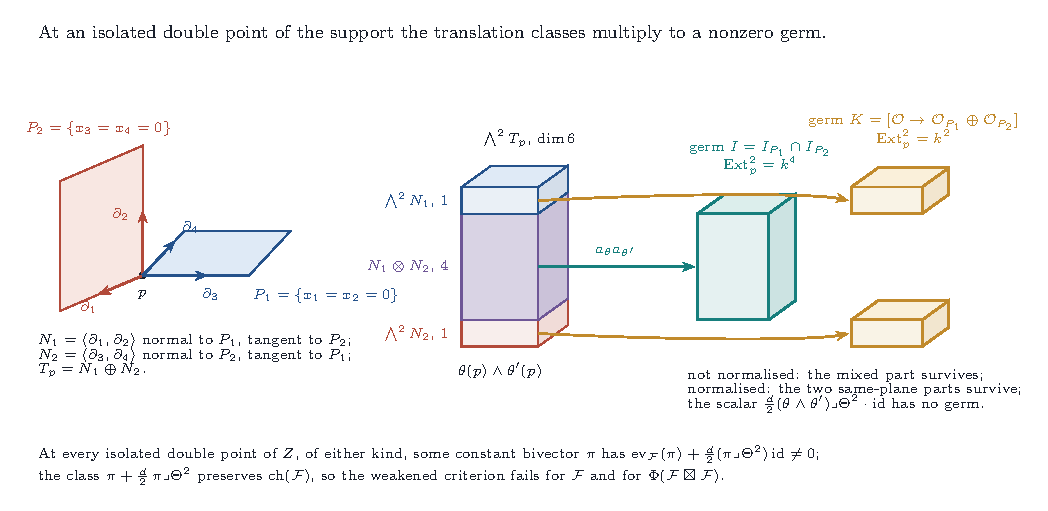
\includegraphics[width=\textwidth]{fig_doublepoint}
\caption{\Cref{lem:localproducts} and \Cref{thm:candidatefails}. Left: two
smooth surfaces of a fourfold meeting transversally at $p$, with the normal
spaces $N_{1}$ and $N_{2}$, each tangent to the other branch. Centre: the
bivectors at $p$, split into $\bigwedge^{2}N_{1}$, $N_{1}\otimes N_{2}$ and
$\bigwedge^{2}N_{2}$, with heights proportional to the dimensions. Right: the
local $\Ext^{2}$ of the germ of $\cF$ at $p$ in the two cases, and the part
of the bivectors that the products of the translation classes carry onto it:
the mixed part when the point is not normalised, the two same-plane parts
when it is. The compensating scalar has no germ, so in either case the
identity \eqref{eq:heisenberg} fails at $p$.}
\label{fig:doublepoint}
\end{figure}

\begin{corollary}[A local obstruction in every dimension]\label{cor:localobstruction}
Let $(X,t)$ be a polarised abelian variety of dimension $n\ge4$ and $F$ a
perfect complex on $X$ with $\ch(F)=au_{t}+bv_{t}$, $(a,b)\ne(0,0)$. Suppose
that at some point $p$ the germ $F_{p}$ is isomorphic, in the derived
category of $\cO_{X,p}$-modules, to the ideal of the union of two smooth germs
of codimension two meeting transversally along a germ of codimension four,
or, when $n=4$, to the complex $[\cO\to\cO_{P_{1}}\oplus\cO_{P_{2}}]$ of two
such germs. Then $F$ does not satisfy the weakened criterion, and neither does
$\Phi(F\boxtimes F_{2})$ on $X\times\widehat X$ for any secant $F_{2}$. In
particular, in every dimension $n\ge4$, the union $Z$ of the intersections
$D_{i}\cap D_{i+1}$ of consecutive translates of a polarisation in general
position contains, for every pair $(i,j)$ of nonconsecutive indices, a
subvariety $Z_{i}\cap Z_{j}$ of codimension four along which $Z$ has two
transversal branches; any secant object of the form $[\cO_{X}\to\nu_{*}\cO_{\widetilde Z}]\otimes L$
in which $\nu$ is an isomorphism at a general point of one such
$Z_{i}\cap Z_{j}$ fails the criterion.
\end{corollary}

\begin{proof}
In formal coordinates $x_{1},\dots,x_{n}$ at $p$ with the two branches
$\{x_{1}=x_{2}=0\}$ and $\{x_{3}=x_{4}=0\}$, which exist because the four
local equations of the branches form part of a regular system of
parameters, the ideal is
$I\otimes_{\CC}\CC[x_{5},\dots,x_{n}]$ with $I$ as in \Cref{lem:localproducts},
and \eqref{eq:kunnethext} with the third factor gives
$\Ext^{2}(I_{p},I_{p})=N_{1}\otimes N_{2}\otimes\cO_{W,p}$, where $W$ is the
intersection of the branches. The jet classes along $\partial_{5},\dots,\partial_{n}$
vanish, since these derivations act on a free factor, and the products of the
classes along $\partial_{1},\dots,\partial_{4}$ are as in the lemma. Reducing
modulo the maximal ideal of $\cO_{W,p}$ shows that $a_{\theta}a_{\theta'}\ne0$
whenever $\theta(p)\wedge\theta'(p)$ has a nonzero component in
$N_{1}\otimes N_{2}$. When $n=4$ and $F_{p}$ is the complex
$[\cO\to\cO_{P_{1}}\oplus\cO_{P_{2}}]$, \Cref{lem:localproducts}(ii) applies
directly. The rest of the argument is that of
\Cref{thm:candidatefails}, using \Cref{thm:factor} for $n\ge3$. For the last
assertion, $Z_{i}\cap Z_{j}=D_{i}\cap D_{i+1}\cap D_{j}\cap D_{j+1}$ is a
transversal intersection of four divisors, of codimension four, and at a
general point of it no fifth divisor passes, so $Z$ has exactly the two
branches $Z_{i}$ and $Z_{j}$ there.
\end{proof}

\begin{remark}[Scope of the local obstruction]\label{rem:candidatemeaning}
\Cref{thm:candidatefails} answers the question posed in
\cite[Section 12]{Mar25b}: the secant objects proposed there do not satisfy
the weakened criterion of \cite[Question 11.4]{Mar25b}, for any
discriminant. The reason is local and geometric. That question asks whether
the semiregularity map may be required to be injective only on the image of
the evaluation map. For a secant object this image contains, by
\Cref{thm:factor}, the products $A_{\theta}A_{\theta'}$ of the translation
classes shifted by the scalars
$\tfrac d2(\theta\wedge\theta')\lrcorner\,\Theta^{2}$, and the
semiregularity map kills them all. For the criterion to hold these shifted
products must vanish, and they cannot: at an isolated double point of the
support, the translation classes of the two branches multiply to a nonzero
local class, while a scalar has no local class at all. The fourth ingredient
of \cite[Remark~14.16]{paperI} can accordingly be stated more sharply. A secant
object of positive rank on a fourfold that satisfies the weakened criterion
must have, at every point, germs whose translation classes multiply to zero
in the local $\Ext^{2}$. By \Cref{lem:localproducts} this excludes every
support with two transversal branches of codimension two through a point,
whether or not the branches are separated, and by
\Cref{cor:localobstruction} it excludes the chain of consecutive
intersections of translates in every dimension. An object supported on a
smooth surface, or on surfaces meeting only along curves, is not excluded by
this argument, but no such object with Chern character on the secant plane
is known.
\end{remark}
\subsection{Smooth supports and four discriminants}
\label{ssec:smoothsupport}

\Cref{thm:candidatefails} and \Cref{cor:localobstruction} exclude every secant
object whose support has two transversal branches of codimension two
through a point. This leaves supports that are smooth or that meet
themselves only along curves, and \Cref{rem:candidatemeaning} ends with the
observation that no such object is known. In this subsection we explain why
the local argument cannot reach the smooth case, and then determine what a
smooth support can be. The answer is narrow: on the fourfold the invariants
of the support are forced, and the discriminant is confined to a finite list.

We begin with the fact that at a smooth point there is nothing local left to
compute.

\begin{proposition}[No local obstruction at a smooth point]\label{prop:smoothlocal}
Let $Y$ be a smooth variety with $\omega_{Y}\cong\cO_{Y}$ and let $S\subset Y$
be smooth of codimension two. Then
\[
  \cE xt^{0}(\cI_{S},\cI_{S})=\cO_{Y},\qquad
  \cE xt^{1}(\cI_{S},\cI_{S})=N_{S/Y},\qquad
  \cE xt^{q}(\cI_{S},\cI_{S})=0\quad(q\ge2),
\]
and the same holds for $\cI_{S}\otimes L$ for any line bundle $L$.
Consequently, for $F=\cI_{S}\otimes L$ both sides of \eqref{eq:heisenberg}
have vanishing germs in $\cE xt^{2}$, and \Cref{lem:edge} decides nothing.
\end{proposition}

\begin{proof}
Twisting by $L$ changes neither side, so take $F=\cI_{S}$. The sheaf
$\cI_{S}$ is torsion free of rank one, and its dual is $\cO_{Y}$ because $S$
has codimension two; hence every local endomorphism of $\cI_{S}$ is
multiplication by a function, and
$\cE xt^{0}(\cI_{S},\cI_{S})=\cO_{Y}$. Apply $\cH om(-,\cI_{S})$ to
\begin{equation}\label{eq:idealseq}
  0\to\cI_{S}\to\cO_{Y}\to\cO_{S}\to0 .
\end{equation}
Since $\cE xt^{q}(\cO_{Y},\cI_{S})=0$ for $q\ge1$, the long exact sequence
gives
\begin{equation}\label{eq:shift}
  \cE xt^{q}(\cI_{S},\cI_{S})\cong\cE xt^{q+1}(\cO_{S},\cI_{S})
  \qquad(q\ge1).
\end{equation}
Now apply $\cH om(\cO_{S},-)$ to \eqref{eq:idealseq}. Because $S$ is smooth of
codimension two, hence a local complete intersection, the Koszul resolution
gives $\cE xt^{k}(\cO_{S},\cO_{Y})=0$ for $k\ne2$ and
$\cE xt^{2}(\cO_{S},\cO_{Y})=\omega_{S}\otimes\omega_{Y}^{-1}=\omega_{S}$,
while $\cE xt^{k}(\cO_{S},\cO_{S})=\bigwedge^{k}N_{S/Y}$ for $0\le k\le2$ and
zero otherwise. Computing both from the same Koszul complex shows that the
map
\[
  \rho\colon\cE xt^{2}(\cO_{S},\cO_{Y})=\omega_{S}
  \longrightarrow
  \cE xt^{2}(\cO_{S},\cO_{S})=\textstyle\bigwedge^{2}N_{S/Y}=\omega_{S}
\]
induced by $\cO_{Y}\to\cO_{S}$ is the identity: in local coordinates in which
$S=\{x_{1}=x_{2}=0\}$, both groups are computed as $M/(x_{1},x_{2})M$ for
$M=\cO_{Y}$ and $M=\cO_{S}$, and the map is reduction modulo $(x_{1},x_{2})$,
which is the identity on $\cO_{S}$.

Consider the long exact sequence of $\cH om(\cO_{S},-)$ in degrees two and
three. Since $\rho$ is surjective and $\cE xt^{3}(\cO_{S},\cO_{Y})=0$, the
segment
\[
  \cE xt^{2}(\cO_{S},\cO_{Y})\xrightarrow{\ \rho\ }
  \cE xt^{2}(\cO_{S},\cO_{S})\to
  \cE xt^{3}(\cO_{S},\cI_{S})\to
  \cE xt^{3}(\cO_{S},\cO_{Y})=0
\]
gives $\cE xt^{3}(\cO_{S},\cI_{S})=0$, so $\cE xt^{2}(\cI_{S},\cI_{S})=0$ by
\eqref{eq:shift}. For $k\ge3$ both $\cE xt^{k}(\cO_{S},\cO_{Y})$ and
$\cE xt^{k}(\cO_{S},\cO_{S})$ vanish, so
$\cE xt^{k+1}(\cO_{S},\cI_{S})=0$ and $\cE xt^{k}(\cI_{S},\cI_{S})=0$. In
degrees one and two, since $\rho$ is injective, the segment
\[
  0=\cE xt^{1}(\cO_{S},\cO_{Y})\to
  N_{S/Y}\to
  \cE xt^{2}(\cO_{S},\cI_{S})\to
  \cE xt^{2}(\cO_{S},\cO_{Y})\xrightarrow{\ \rho\ }
  \cE xt^{2}(\cO_{S},\cO_{S}),
\]
in which $N_{S/Y}=\cE xt^{1}(\cO_{S},\cO_{S})$, gives
$\cE xt^{2}(\cO_{S},\cI_{S})\cong N_{S/Y}$, and this is
$\cE xt^{1}(\cI_{S},\cI_{S})$ by \eqref{eq:shift}.

For the last assertion, the right side of \eqref{eq:heisenberg} has vanishing
germs by \Cref{lem:edge}, and the left side lies in
$\Ext^{2}(F,F\otimes\Omega^{2}_{Y})$, whose sheaf of germs in the
$\cE xt^{2}$ direction is $\cE xt^{2}(F,F)\otimes\Omega^{2}_{Y}=0$.
\end{proof}

\begin{remark}[The global form of the criterion]\label{rem:obstructionmoves}
\Cref{prop:smoothlocal} is the precise reason why the argument of
\Cref{thm:candidatefails} stops at a smooth support, and it also shows what
takes its place. Since $\cE xt^{2}=0$, the local-to-global spectral sequence
for $\Ext^{2}(\cI_{S},\cI_{S})$ has only two surviving rows,
$H^{1}(S,N_{S/Y})$ and $H^{2}(Y,\cO_{Y})$, and they sit in different steps of
the filtration: the first is the quotient that records the geometry of $S$,
the second the subgroup of scalars. A product $A_{\theta}A_{\theta'}$ of
translation classes therefore has a well defined image in $H^{1}(S,N_{S/Y})$,
while the scalar on the right of \eqref{eq:heisenberg} has image zero there.
The criterion thus splits into two conditions of different kinds: a vanishing
in $H^{1}(S,N_{S/Y})$, which is a statement about the normal bundle and not
about any point, and an identity in $H^{2}(Y,\cO_{Y})$. At a double point the
first condition already fails locally. At a smooth support it is a global
question, and what is decided here is which surfaces $S$ are available at
all.
\end{remark}

The invariants of a smooth support are far from free. Since the Todd class of
an abelian variety is trivial, Grothendieck--Riemann--Roch converts the Chern
character of the object into the complete set of numerical invariants of the
surface, and three classical inequalities then constrain them.

\begin{theorem}[The invariants of a smooth support]\label{thm:smoothinvariants}
Let $(X,\Theta)$ be a principally polarised abelian fourfold, let $d>0$, let
$b\in\ZZ_{>0}$, and let $\cF=\cI_{S}(b\Theta)$ be a coherent sheaf with
\[
  \ch(\cF)=u_{\Theta}+b\,v_{\Theta}
\]
and $S\subset X$ smooth. Write $N=\tfrac12\Nm_{K/\QQ}(b+\sqrt{-d})
=\tfrac12(b^{2}+d)$, $\iota\colon S\hookrightarrow X$ and
$\lambda=\iota^{*}\Theta$. Then $S$ is a surface and
\begin{equation}\label{eq:smoothinvariants}
\begin{aligned}
  [S]&=N\Theta^{2}, &\qquad \iota_{*}K_{S}&=\tfrac{4bN}{3}\,\Theta^{3},
  &\qquad \chi(\cO_{S})&=4N(2b^{2}-N),\\
  K_{S}^{2}&=12N(4b^{2}-N), &\qquad e(S)&=12N(4b^{2}-3N),
  &\qquad K_{S}\cdot\lambda&=32bN,
\end{aligned}
\end{equation}
with $\lambda^{2}=24N$ and $[S]^{2}=24N^{2}$. Moreover $K_{S}$ is globally
generated, hence nef; $S$ is minimal of general type; and
\begin{equation}\label{eq:threebounds}
  \tfrac{4}{9}b^{2}\ \le\ N\ \le\ b^{2},
  \qquad\text{equivalently}\qquad
  -\tfrac{1}{9}b^{2}\ \le\ d\ \le\ b^{2} .
\end{equation}
The lower bound is the Hodge index theorem and is implied by $d>0$; the upper
bound is the Bogomolov--Miyaoka--Yau inequality. In terms of $b$ and $d$ the
five invariants read
\begin{equation}\label{eq:bdform}
  \chi(\cO_{S})=(b^{2}+d)(3b^{2}-d),\quad
  K_{S}^{2}=3(b^{2}+d)(7b^{2}-d),\quad
  e(S)=3(b^{2}+d)(5b^{2}-3d),
\end{equation}
and the defect in the Bogomolov--Miyaoka--Yau inequality is
\begin{equation}\label{eq:bmydefect}
  3e(S)-K_{S}^{2}=24\,(b^{4}-d^{2}),
\end{equation}
so that the inequality amounts exactly to $d\le b^{2}$.
Finally, $K_{S}$ is never numerically proportional to $\lambda$.
\end{theorem}

\begin{proof}
Since $\ch_{0}(\cF)=1$ and $c_{1}(\cF)=b\Theta$, the sheaf
$\cF(-b\Theta)=\cI_{S}$ has $\ch_{0}=1$, $\ch_{1}=0$, so $S$ has codimension
at least two, and
\[
  \ch(\cO_{S})=1-\ch(\cI_{S})=1-\ch(\cF)\,e^{-b\Theta}.
\]
Put $z=b+\sqrt{-d}$, so that $z\bbar z=2N$. Since
$u_{\Theta}=\Re e^{\sqrt{-d}\Theta}$ and
$\sqrt d\,v_{\Theta}=\Im e^{\sqrt{-d}\Theta}$, we have
$\ch(\cF)=\Im\bigl(z\,e^{\sqrt{-d}\Theta}\bigr)/\sqrt d$, hence
$\ch(\cF)e^{-b\Theta}=\Im\bigl(z\,e^{-\bbar z\Theta}\bigr)/\sqrt d$, whose
coefficient of $\Theta^{k}$ is
$(-1)^{k}\Im(z\bbar z^{k})/(\sqrt d\,k!)=(-1)^{k+1}\,2N\Im(z^{k-1})/(\sqrt d\,k!)$.
With $\Im z=\sqrt d$, $\Im z^{2}=2b\sqrt d$ and
$\Im z^{3}=(3b^{2}-d)\sqrt d$ this gives
\[
  \ch_{2}(\cO_{S})=\tfrac{b^{2}+d}{2}\Theta^{2}=N\Theta^{2},\quad
  \ch_{3}(\cO_{S})=-\tfrac{2bN}{3}\Theta^{3},\quad
  \ch_{4}(\cO_{S})=\tfrac{3b^{4}+2db^{2}-d^{2}}{24}\Theta^{4}.
\]
The first
identity says $S$ has codimension exactly two, so it is a surface, with class
$N\Theta^{2}$. Because $T_{X}$ is trivial, $\td(T_{X})=1$, and
Grothendieck--Riemann--Roch for $\iota$ reads
$\ch(\iota_{*}\cO_{S})=\iota_{*}\td(T_{S})$. Comparing degrees three and four,
\[
  \ch_{3}(\cO_{S})=\iota_{*}\tfrac{c_{1}(T_{S})}{2}=-\tfrac12\iota_{*}K_{S},
  \qquad
  \ch_{4}(\cO_{S})=\iota_{*}\tfrac{c_{1}^{2}+c_{2}}{12}
  =\chi(\cO_{S})\,[\mathrm{pt}],
\]
the second by Noether's formula. With $\Theta^{4}=24\,[\mathrm{pt}]$ these give
$\iota_{*}K_{S}=\tfrac{4bN}{3}\Theta^{3}$ and, after substituting
$d=2N-b^{2}$, $\chi(\cO_{S})=3b^{4}+2db^{2}-d^{2}=4N(2b^{2}-N)$.
Then $K_{S}\cdot\lambda=\int_{X}\iota_{*}K_{S}\cdot\Theta=\tfrac{4bN}{3}\cdot24=32bN$
and $\lambda^{2}=\int_{X}[S]\cdot\Theta^{2}=24N$.

For the last two invariants, the normal bundle sequence and the triviality of
$T_{X}$ give $c(T_{S})c(N_{S/X})=1$, so $c_{1}(N_{S/X})=K_{S}$ and
$c_{2}(N_{S/X})=K_{S}^{2}-e(S)$; the self-intersection formula
$[S]^{2}=\int_{S}c_{2}(N_{S/X})$ then reads
\[
  24N^{2}=K_{S}^{2}-e(S),
\]
while Noether's formula reads $12\chi(\cO_{S})=K_{S}^{2}+e(S)$. Solving the
two gives the stated $K_{S}^{2}$ and $e(S)$.

The conormal sequence presents $\Omega^{1}_{S}$ as a quotient of
$\Omega^{1}_{X}|_{S}=\cO_{S}^{\oplus4}$, so $\Omega^{1}_{S}$ is globally
generated, and therefore so is $K_{S}=\det\Omega^{1}_{S}$, a quotient of
$\bigwedge^{2}\cO_{S}^{\oplus4}$. A globally generated line bundle is nef. A
globally generated rank two bundle on a surface has $c_{2}\ge0$, the class
$c_{2}$ being represented by the vanishing scheme of a general section, which
is empty or finite; hence
\[
  e(S)=c_{2}(\Omega^{1}_{S})=12N(4b^{2}-3N)\ \ge\ 0,
\]
so $N\le\tfrac43b^{2}<4b^{2}$ and therefore $K_{S}^{2}=12N(4b^{2}-N)>0$. A nef
divisor of positive self-intersection is big, so $\kappa(S)=2$ and, $K_{S}$
being nef, $S$ is minimal of general type. The Bogomolov--Miyaoka--Yau
inequality $c_{1}^{2}\le3c_{2}$ therefore applies and reads
$K_{S}^{2}\le3e(S)$. Substituting $N=\tfrac12(b^{2}+d)$ in
\eqref{eq:smoothinvariants} gives \eqref{eq:bdform}, hence
$3e(S)-K_{S}^{2}=24(b^{4}-d^{2})$, and the inequality is $d\le b^{2}$, that
is $N\le b^{2}$.

For the lower bound, $\lambda$ is ample on $S$, so the Hodge index theorem
gives $(K_{S}\cdot\lambda)^{2}\ge K_{S}^{2}\,\lambda^{2}$, that is
$(32bN)^{2}\ge12N(4b^{2}-N)\cdot24N$, which simplifies to $9N\ge4b^{2}$. Since
$N=\tfrac12(b^{2}+d)$ with $d>0$, this holds automatically. Equality in the
Hodge index theorem occurs exactly when $K_{S}$ is numerically proportional to
$\lambda$, hence exactly when $9N=4b^{2}$, and this never happens, because
$9N=\tfrac92(b^{2}+d)>4b^{2}$ for $d>0$.
\end{proof}

\Cref{fig:bmywindow} draws the Bogomolov--Miyaoka--Yau defect over the
quarter plane of $(b,d)$.

\begin{corollary}[Four discriminants on the fourfold]\label{cor:fourdiscriminants}
Let $(X,\Theta)$ be a principally polarised abelian fourfold and $d>0$
squarefree. A sheaf $\cI_{S}(3\Theta)$ with Chern character
$u_{\Theta}+3v_{\Theta}$, the value of \Cref{prop:markman8}(iii), and with
smooth support $S$ exists only if $d\le9$, that is
$d\in\{1,2,3,5,6,7\}$; if in addition $N=(9+d)/2$ is an integer, as in
\Cref{setup:markman}, only
\[
  d\in\{1,\,3,\,5,\,7\},\qquad N\in\{5,\,6,\,7,\,8\}.
\]
For these values the invariants are forced to be those of
\Cref{tab:smoothsupport}. In particular, for $d>9$ no such sheaf has smooth
support.
\end{corollary}

\begin{proof}
This is immediate from \eqref{eq:threebounds} at $b=3$ and the arithmetic of
\eqref{eq:smoothinvariants}, and the table evaluates
\eqref{eq:smoothinvariants} at $b=3$. The value $d=9$ is the equality case of the
Bogomolov--Miyaoka--Yau inequality, where $K_{S}^{2}=3e(S)=2916$ and $S$ would
have to be a quotient of the ball; it is excluded because $9$ is not
squarefree.
\end{proof}

\begin{table}[htbp]
\centering
\small
\renewcommand{\arraystretch}{1.12}
\begin{tabular}{@{}ccrrrrr@{}}
\toprule
$d$ & $N$ & $\chi(\cO_{S})$ & $K_{S}^{2}$ & $e(S)$ &
$K_{S}\cdot\lambda$ & $\lambda^{2}$ \\
\midrule
$1$ & $5$ & $260$ & $1860$ & $1260$ & $480$ & $120$ \\
$3$ & $6$ & $288$ & $2160$ & $1296$ & $576$ & $144$ \\
$5$ & $7$ & $308$ & $2436$ & $1260$ & $672$ & $168$ \\
$7$ & $8$ & $320$ & $2688$ & $1152$ & $768$ & $192$ \\
\bottomrule
\end{tabular}
\caption{The only invariants a smooth support can have on an abelian
fourfold, by \Cref{thm:smoothinvariants} and
\Cref{cor:fourdiscriminants}, at $b=3$ and with $N$ an integer. Every entry is
determined by $\ch(\cF)$ alone. The slope
$K_{S}^{2}/\chi(\cO_{S})$ runs from $93/13$ at $d=1$ to $42/5$ at $d=7$, and
reaches the Bogomolov--Miyaoka--Yau ceiling of $9$ only at the excluded value
$d=9$.}
\label{tab:smoothsupport}
\end{table}

\begin{figure}[htbp]
\centering
  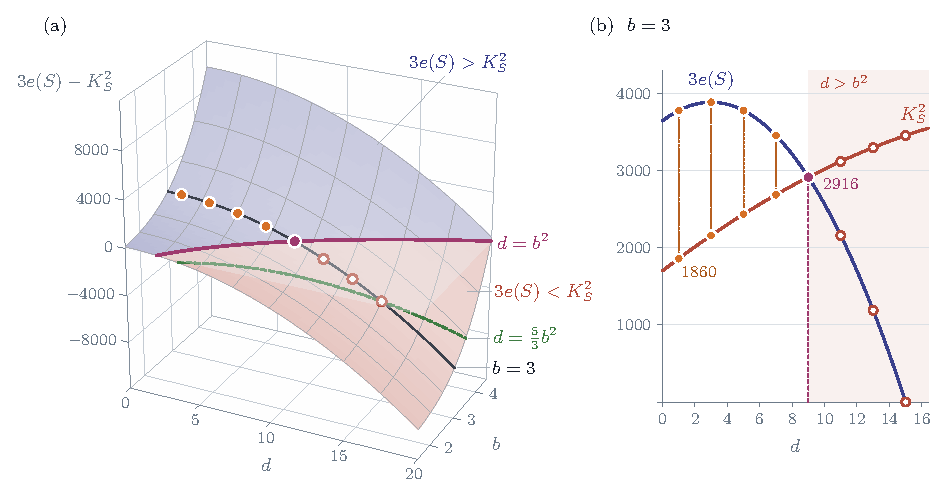
\includegraphics[width=\textwidth]{fig_bmywindow}
\caption{\Cref{thm:smoothinvariants} over the quarter plane of $(b,d)$. The
height of the surface is the defect $3e(S)-K_{S}^{2}=24(b^{4}-d^{2})$ in the
Bogomolov--Miyaoka--Yau inequality for the surface the theorem attaches to the
pair, compressed by a signed cube root so that four orders of magnitude fit
one frame; the compression is odd and monotone, so the zero locus and the sign
are the true ones. The surface is drawn indigo where the defect is positive and
clay where it is negative, and it crosses zero along $d=b^{2}$, which is
therefore the whole content of the inequality. The weaker wall $d=\tfrac53
b^{2}$, where $e(S)$ itself changes sign, is drawn dashed and lies above it.
On the line $b=3$, which is the value \Cref{prop:markman8}(iii) forces on the
fourfold, the four squarefree discriminants $d=1,3,5,7$ with $N$ an integer sit
above the wall and are marked with their drop lines; $d=9$ sits exactly on it,
the equality case, and $d=11,13,15$ sit below and are excluded.}
\label{fig:bmywindow}
\end{figure}

\begin{remark}[Status of the smooth case]\label{rem:smoothremains}
The local argument does not apply here, for a structural reason given by
\Cref{prop:smoothlocal}: the sheaf $\cE xt^{2}$ of a smooth ideal vanishes,
so both sides of \eqref{eq:heisenberg} are locally zero, and the comparison of
germs that decides \Cref{thm:candidatefails} has nothing to compare.

The surface is rigidly constrained. At $b=3$ its class, its canonical class,
its Euler characteristic, its Euler number and its two intersection numbers
with the polarisation are all determined by $d$, and they are compatible with
existence only for $d\le9$. This is the content of
\Cref{cor:fourdiscriminants}, and it restricts the construction: for all but
finitely many imaginary quadratic fields the secant construction of
\Cref{setup:markman} with smooth support is not available, whatever the
geometry of the surface.

What remains is a single existence question. For $d\in\{1,3,5,7\}$, does a
principally polarised abelian fourfold carry a smooth surface $S$ with the
invariants of \Cref{tab:smoothsupport}, and if so, does the image of
$A_{\theta}A_{\theta'}$ in $H^{1}(S,N_{S/X})$ vanish for all
$\theta,\theta'\in H^{0}(T_{X})$? The first half is a question about surfaces
in abelian fourfolds with prescribed Chern numbers, of the kind that is
answered by a construction or by a classification argument; the second is a
question about one cohomology group of one normal bundle. Neither is settled
here. The simplest surfaces of the right class are ruled out by one entry of
the table: a complete intersection of divisors in $|a\Theta|$ and
$|b'\Theta|$ has class $ab'\Theta^{2}$, so $ab'=N$, and canonical class
$(a+b')\lambda$ by adjunction, so $K_{S}\cdot\lambda=24(a+b')N$; since
$ab'=N\ge5$ forces $a+b'\ge5$, this exceeds the required $96N$. The
surface, if it exists, is not cut out by two theta divisors, nor by any two
divisors algebraically equivalent to multiples of $\Theta$; nor, by
\Cref{cor:latticeburch} below, is its ideal sheaf presented by any two bundles
whose classes lie in the subring generated by line bundles. It must also move
with $X$ to first order in every polarised direction, in the exact sense of
\Cref{prop:smoothrank}, while the injectivity that \Cref{lem:annihilation}
asks of it holds automatically when $X$ is simple (\Cref{lem:smoothinjective}).

A positive answer to both, for a surface that moves in this way, together
with an affirmative answer to \cite[Question 11.4]{Mar25b}, would produce
Weil classes on abelian
eightfolds for at most four discriminants; the other discriminants, every
$n\ge5$ and every field of degree larger than two would still have to be
reached through \cite[Proposition~2.13]{paperIII} and the propagation statement.
\end{remark}

Two of the conditions on a smooth support are decided by the table, and the
third, which \Cref{thm:factor}(iii)(a) imposes on every candidate, has an
exact form. The first is the injectivity of $H^{2}(\cO_{X})\to H^{2}(\cO_{S})$
that \Cref{lem:annihilation} below requires of every support.

\begin{lemma}[The injectivity condition for a smooth support]
\label{lem:smoothinjective}
Let $X$ be a simple complex abelian fourfold, let $V=H^{0}(T_{X})$, and let
$S\subset X$ be a smooth surface. The following are equivalent:
\begin{enumerate}[label=\textup{(\roman*)},nosep,leftmargin=2.2em]
\item the restriction $H^{2}(\cO_{X})\to H^{2}(\cO_{S})$ is injective;
\item no nonzero translation-invariant holomorphic $2$-form on $X$ restricts
  to zero on $S$;
\item $S$ is not Lagrangian for any translation-invariant holomorphic
  symplectic form on $X$;
\item the Gauss image of $S$ in $\operatorname{Gr}(2,V)\subset\PP(\bigwedge^{2}V)$
  spans $\PP(\bigwedge^{2}V)$.
\end{enumerate}
If $e(S)\ne[S]^{2}$, they hold. In particular they hold for every smooth
support of \Cref{tab:smoothsupport}, where $e(S)=12N(36-3N)$ and
$[S]^{2}=24N^{2}$ agree only for $5N=36$.
\end{lemma}

\begin{proof}
The restriction $\iota^{*}\colon H^{2}(X,\CC)\to H^{2}(S,\CC)$ is a morphism
of Hodge structures defined over $\QQ$, so it commutes with complex
conjugation, which interchanges the $(0,2)$ and $(2,0)$ parts; hence
$\iota^{*}$ is injective on $H^{0,2}(X)=H^{2}(\cO_{X})$ if and only if it is
injective on $H^{2,0}(X)=\bigwedge^{2}V^{\vee}$, the translation-invariant
$2$-forms. A holomorphic $2$-form on a compact surface is zero as a class in
$H^{2,0}(S)=H^{0}(K_{S})$ if and only if it is zero as a form; this is
(i)$\Leftrightarrow$(ii). The restriction of $p\wedge q\in\bigwedge^{2}V^{\vee}$
to $S$ is the pull-back of the Pl\"ucker coordinate $p\wedge q$ along the
Gauss map $\gamma\colon S\to\operatorname{Gr}(2,V)$, $s\mapsto T_{s}S$, as a
section of $K_{S}=\gamma^{*}\cO(1)$, so a $2$-form vanishes on $S$ if and
only if the corresponding hyperplane contains $\gamma(S)$; this is
(ii)$\Leftrightarrow$(iv).

A nonzero $2$-form on $V\cong\CC^{4}$ has rank two or four. If $\omega$ has
rank four, $\omega|_{S}=0$ says that every tangent plane of $S$ is
$\omega$-isotropic, that is, $S$ is Lagrangian for $\omega$. If
$\omega=\alpha\wedge\beta$ has rank two, with $\alpha,\beta\in V^{\vee}$
independent, then $\alpha|_{S}$ and $\beta|_{S}$ are independent
holomorphic $1$-forms on $S$, because $S$ generates the simple $X$ and a nonzero
invariant $1$-form restricts nontrivially to a generating subvariety, and
$\alpha|_{S}\wedge\beta|_{S}=0$. By the theorem of Castelnuovo and de
Franchis \cite{BHPV04} there is a fibration
$f\colon S\to C$ onto a curve of genus at least two with $\alpha|_{S}$ and
$\beta|_{S}$ pulled back from $C$. A fibre $F$ of $f$ is a curve in $X$ on
which $\alpha$ and $\beta$ vanish, so all its tangent lines lie in the fixed
plane $B=\ker\alpha\cap\ker\beta\subset V$. The abelian subvariety generated
by $F-F$ is the image of a sum map from a power of $F$, whose differential at
a general point is spanned by tangent vectors of $F$; so its tangent space
lies in $B$, its dimension is at most two, and it is nonzero because $F$ is
not a point. This contradicts the simplicity of $X$. Hence only the
rank-four case occurs, which is (ii)$\Leftrightarrow$(iii).

Finally, if $S$ is Lagrangian for a symplectic $\omega$, then $\omega$
identifies $T_{S}$ with the annihilator of $T_{S}$ in $\Omega^{1}_{X}|_{S}$,
which is the conormal bundle, so $N_{S/X}\cong\Omega^{1}_{S}$ and
$c_{2}(N_{S/X})=e(S)$; since $T_{X}$ is trivial, $c_{2}(N_{S/X})=[S]^{2}$ by
the self-intersection formula. So $e(S)\ne[S]^{2}$ excludes (iii). For the
table, \Cref{thm:smoothinvariants} gives $[S]^{2}=24N^{2}$ and
$e(S)=12N(36-3N)$ at $b=3$, and $24N^{2}=12N(36-3N)$ reads $5N=36$. For
general $b$ the two agree only when $N=\tfrac45b^{2}$, that is
$d=\tfrac35b^{2}$, whose first integral instance is $b=5$, $d=15$.
\end{proof}

\begin{remark}[The class $K_{S}-4\lambda$]\label{rem:gysinkernel}
\Cref{thm:smoothinvariants} records $K_{S}\cdot\lambda=96N$ and
$\lambda^{2}=24N$ at $b=3$, so $K_{S}\cdot\lambda=4\lambda^{2}$, and that
$K_{S}$ is never numerically proportional to $\lambda$. The sharper
statement is that
\[
  \delta=K_{S}-4\lambda\in\ker\bigl(\iota_{*}\colon H^{2}(S,\QQ)\to H^{6}(X,\QQ)\bigr),
  \qquad \delta^{2}=-12N(N-4)<0,
\]
because $\iota_{*}K_{S}=4N\Theta^{3}$ and
$\iota_{*}\lambda=\Theta\cup[S]=N\Theta^{3}$. So $\delta$ is a nonzero
algebraic class of type $(1,1)$, orthogonal by the projection formula to the
whole image of $H^{2}(X,\QQ)$ in $H^{2}(S,\QQ)$, and of negative square: the
Picard number of $S$ is at least two, and the kernel of the Gysin map on
$H^{2}(S,\QQ)$, a sub-Hodge structure, contains an algebraic class. For
general $b$ the class is $K_{S}-\tfrac{4b}{3}\lambda$, with square
$\tfrac{4N}{3}(4b^{2}-9N)$, and its vanishing is the equality case $9N=4b^{2}$
of the Hodge index bound in \Cref{thm:smoothinvariants}. This excludes none
of the four cases; it describes them.
\end{remark}

The third condition is the one that \Cref{thm:factor}(iii)(a) imposes on
every candidate and that the construction of \Cref{setup:markman} meets by
its uniformity over the moduli of principally polarised fourfolds
(\Cref{cor:markmancondition}): the object must extend to first order along
every polarised deformation of $(X,\Theta)$. For $\cF=\cI_{S}(3\Theta)$ with
$S$ smooth this is a condition on $S$. If $S$ extends along a deformation
$X_{v}$ of $X$ that keeps $\Theta$ of type $(1,1)$, then so does $\cF$.
Conversely, the obstruction $v\lrcorner\,\mathrm{At}(\cF)\in\Ext^{2}(\cF,\cF)$
has, under the edge map to $H^{1}(S,\cE xt^{1}(\cF,\cF))=H^{1}(S,N_{S/X})$ of
\Cref{rem:obstructionmoves}, the image of $v$ under
$H^{1}(T_{X})\to H^{1}(\iota^{*}T_{X})\to H^{1}(N_{S/X})$, by
\Cref{lem:edge} applied on the overlaps of a cover; and that image is the
obstruction $\operatorname{ob}_{S}(v)$ to extending the subscheme $S$ along
$X_{v}$. So condition (a) for $\cF$ is the statement that $S$ extends to
first order along every polarised deformation of $X$, and Bloch's
semiregularity map \cite{Blo72} puts it in a form that names the object it
concerns. For $S\subset X$ smooth of codimension two with normal bundle
$N=N_{S/X}$, let
\[
  \pi\colon H^{1}(S,N)\xrightarrow{\ \cong\ }H^{1}(S,N^{\vee}\otimes K_{S})
  \xrightarrow{\ j\ }H^{1}(S,\iota^{*}\Omega^{1}_{X}\otimes K_{S})
  \xrightarrow{\ \iota_{*}\ }H^{3}(X,\Omega^{1}_{X})
\]
be the composite of $N\cong N^{\vee}\otimes\bigwedge^{2}N$, of the conormal
inclusion $N^{\vee}\to\iota^{*}\Omega^{1}_{X}$ tensored with $K_{S}$, and of
the Gysin map, with $K_{X}\cong\cO_{X}$. This is the semiregularity map of
Bloch for codimension two, and it satisfies
$\pi(\operatorname{ob}_{S}(v))=v\lrcorner[S]$ for every $v\in H^{1}(X,T_{X})$.

\begin{lemma}[Duality]\label{lem:blochduality}
Under Serre duality $H^{1}(X,T_{X})\times H^{3}(X,\Omega^{1}_{X})\to H^{4}(\cO_{X})=\CC$,
\[
  \{v\in H^{1}(X,T_{X}):S\ \text{extends to first order along }v\}
  =\pi\bigl(H^{1}(S,N)\bigr)^{\perp}.
\]
\end{lemma}

\begin{proof}
$S$ extends along $v$ if and only if $\operatorname{ob}_{S}(v)=0$, and
$\operatorname{ob}_{S}$ is the composite of the restriction
$r\colon H^{1}(X,T_{X})\to H^{1}(S,\iota^{*}T_{X})$ with the map induced by
$\iota^{*}T_{X}\to N$. The Serre dual of $r$ is the Gysin map
$\iota_{*}\colon H^{1}(S,\iota^{*}\Omega^{1}_{X}\otimes K_{S})\to H^{3}(X,\Omega^{1}_{X}\otimes K_{X})$,
and the Serre dual of $H^{1}(\iota^{*}T_{X})\to H^{1}(N)$ is the map
$H^{1}(N^{\vee}\otimes K_{S})\to H^{1}(\iota^{*}\Omega^{1}_{X}\otimes K_{S})$
induced by the conormal inclusion. So the dual of $\operatorname{ob}_{S}$ is
$\iota_{*}\circ j$, which is $\pi$ after the identification
$N\cong N^{\vee}\otimes K_{S}$, and the kernel of a linear map is the
annihilator of the image of its dual.
\end{proof}

\begin{proposition}[The first-order condition is a rank condition]
\label{prop:smoothrank}
Let $S\subset X$ be a smooth surface with $[S]=N\Theta^{2}$, $N\ne0$. Then
$\pi(H^{1}(S,N))\supseteq\Theta\cup H^{0,2}(X)$, a subspace of dimension six,
and the following are equivalent:
\begin{enumerate}[label=\textup{(\roman*)},nosep,leftmargin=2.2em]
\item $S$ extends to first order along every polarised deformation of
  $(X,\Theta)$, that is, $\cI_{S}(3\Theta)$ satisfies condition (a) of
  \Cref{thm:factor}(iii);
\item $\pi(H^{1}(S,N))=\Theta\cup H^{0,2}(X)$;
\item $\operatorname{rank}\pi=6$, the least value possible.
\end{enumerate}
In particular a smooth secant support is as far from semiregular in Bloch's
sense as a surface with this class can be: $\dim\ker\pi=h^{1}(N)-6$, with
$h^{1}(N)=2h^{0}(N)-2\chi(\cO_{S})+24N^{2}\ge8-2\chi(\cO_{S})+24N^{2}$, which
is at least $88$, $296$, $568$ and $904$ for $N=5,6,7,8$.
\end{proposition}

\begin{proof}
The polarised deformations form $P=\{v:v\lrcorner\Theta=0\}$, of dimension
ten in $H^{1}(T_{X})=V\otimes H^{0,1}(X)$. For $z\in H^{0,2}(X)$ the pairing
is $\langle v,\Theta\cup z\rangle=(v\lrcorner\Theta)\cup z$, so
$\Theta\cup H^{0,2}(X)\subseteq P^{\perp}$; the map $z\mapsto\Theta\cup z$ is
injective by hard Lefschetz, so this subspace has dimension six, and
$\dim P^{\perp}=16-10=6$, so $P^{\perp}=\Theta\cup H^{0,2}(X)$. By
\Cref{lem:blochduality}, (i) says $P\subseteq\pi(H^{1}(N))^{\perp}$, that is
$\pi(H^{1}(N))\subseteq P^{\perp}$. On the other hand
$\pi(\operatorname{ob}_{S}(v))=v\lrcorner[S]=2N\,\Theta\cup(v\lrcorner\Theta)$,
and $v\mapsto v\lrcorner\Theta$ is surjective onto $H^{0,2}(X)$, because
$\Theta$ identifies $V$ with $\overline{V}^{\vee}$ and the contraction becomes
the exterior product $V\otimes\overline{V}^{\vee}\to\bigwedge^{2}\overline{V}^{\vee}$.
So $\pi(H^{1}(N))\supseteq\Theta\cup H^{0,2}(X)$ always, and (i), (ii), (iii)
are equivalent. For $h^{1}(N)$, Riemann--Roch with $c_{1}(N)=K_{S}$ and
$c_{2}(N)=[S]^{2}=24N^{2}$ gives $\chi(N)=2\chi(\cO_{S})-24N^{2}$, Serre
duality with $N^{\vee}\otimes K_{S}\cong N$ gives $h^{2}(N)=h^{0}(N)$, and
$h^{0}(N)\ge4$ because the four translation vector fields map injectively to
$H^{0}(N)$: a translation vector field tangent to $S$ everywhere would restrict
to a nowhere vanishing vector field on $S$, so that $e(S)=c_{2}(T_{S})=0$,
while a secant support has $e(S)=12N(36-3N)\ne0$ for $N=5,6,7,8$ by
\Cref{thm:smoothinvariants}.
\end{proof}

\begin{remark}[What the rank condition asks]\label{rem:smoothrank}
\Cref{prop:smoothrank} does not decide the condition; it converts it into the
statement that the kernel of Bloch's map has codimension exactly six, as it
has for the complete intersections $\Theta\cap\Theta_{x}$, which do move with
$X$. The kernel of $\pi$ is
$j^{-1}\bigl(V^{\vee}\otimes\ker(H^{1}(K_{S})\to H^{3}(\cO_{X}))\bigr)$, and
for $q(S)=4$ it is the image in $H^{1}(N^{\vee}\otimes K_{S})$ of
$H^{0}(\Omega^{1}_{S}\otimes K_{S})$ modulo $V^{\vee}\otimes H^{0}(K_{S})$. A
count with $\chi(\Omega^{1}_{S}\otimes K_{S})=2\chi(\cO_{S})+24N^{2}$ and
$h^{1}(T_{S})\le h^{0}(N)+12$ shows the rank condition to be consistent with
every inequality available, so no exclusion follows at this level; what
would decide it is $\ker\pi$ for an actual surface, and no candidate surface
is known.
\end{remark}

\subsection{Depth and the local obstruction}
\label{ssec:depth}

By \Cref{prop:smoothlocal}, at a smooth point of the support there is
nothing local to compare. This is a special case of a much more general
statement, and the general statement shows exactly which supports
\Cref{thm:candidatefails} and \Cref{cor:localobstruction} exclude and which
lie beyond their reach. The dividing line is neither smoothness nor the local
complete intersection property, but depth.

\begin{theorem}[Cohen--Macaulay supports carry no local obstruction]%
\label{thm:cmvanishing}
Let $Y$ be a smooth variety with $\omega_{Y}\cong\cO_{Y}$, let $Z\subset Y$ be
a closed subscheme of codimension two, and let $p\in Z$. If the local ring
$\cO_{Z,p}$ is Cohen--Macaulay, then
\[
  \cE xt^{q}(\cI_{Z},\cI_{Z})_{p}=0\qquad\text{for every }q\ge2 ,
\]
and the same holds for $\cI_{Z}\otimes L$ for every line bundle $L$.
Consequently both sides of \eqref{eq:heisenberg} have vanishing germ at $p$,
and \Cref{lem:edge} decides nothing there.
\end{theorem}

\begin{proof}
Twisting by $L$ changes no $\cE xt$ sheaf, so take $F=\cI_{Z}$. Write
$A=\cO_{Y,p}$, a regular local ring of dimension $m$, and $I=\cI_{Z,p}$. By
hypothesis $A/I$ is Cohen--Macaulay of dimension $m-2$, so
$\operatorname{depth}A/I=m-2$, and the Auslander--Buchsbaum formula gives
\[
  \operatorname{pd}_{A}(A/I)=m-\operatorname{depth}_{A}(A/I)=2 .
\]
From the exact sequence $0\to I\to A\to A/I\to0$ with $A$ free it follows that
$\operatorname{pd}_{A}I=1$. A module of projective dimension one has a free
resolution of length one, so $\Ext^{q}_{A}(I,M)=0$ for every $A$-module $M$
and every $q\ge2$; taking $M=I$ gives the vanishing, since
$\cE xt^{q}(\cI_{Z},\cI_{Z})_{p}=\Ext^{q}_{A}(I,I)$. The last assertion
follows from \Cref{lem:edge}: the right side of \eqref{eq:heisenberg} is
$z\cdot\id_{F}$ with $z\in H^{2}(\cO_{Y})$ and has vanishing germs, and the
left side lies in a sheaf whose $\cE xt^{2}$ factor is zero.
\end{proof}

\begin{remark}[Sharpness of the hypothesis]%
\label{rem:cmsharp}
Two observations show that \Cref{thm:cmvanishing} is the right statement.

First, Cohen--Macaulayness is strictly weaker than the more familiar
conditions that could be imposed instead. Among codimension two germs in
$\CC^{4}$, the smooth germ $(x_{1},x_{2})$, two planes meeting along a line,
$(x_{1},x_{2}x_{3})$, three planes meeting along a line,
$(x_{1},x_{2}x_{3}x_{4})$, the double plane $(x_{1}^{2},x_{2})$ and the
quadric cone $(x_{1},x_{2}^{2}-x_{3}x_{4})$ are complete intersections. The
fat plane $(x_{1},x_{2})^{2}$ and the cone over the twisted cubic are the
ideals of $2\times2$ minors of
$\left(\begin{smallmatrix}x_{1}&x_{2}&0\\
0&x_{1}&x_{2}\end{smallmatrix}\right)$ and of
$\left(\begin{smallmatrix}x_{1}&x_{2}&x_{3}\\
x_{2}&x_{3}&x_{4}\end{smallmatrix}\right)$, of the expected codimension two,
so they are Cohen--Macaulay by the Hilbert--Burch theorem, although neither
is a local complete intersection, both needing three generators. By
\Cref{thm:cmvanishing}, $\cE xt^{2}(\cI_{Z},\cI_{Z})$ vanishes at all seven.
Reducedness, irreducibility and the complete intersection property are
therefore all irrelevant; what matters is the projective dimension, which by
Auslander--Buchsbaum is a matter of depth.

Second, the vanishing fails at the germs that the construction of
\Cref{setup:markman} produces. Two planes meeting at a point and three planes
meeting pairwise at a point are reduced surface germs that become
disconnected when the point is removed, so they have depth $1$: at least $1$
because they are reduced, and at most $1$ by the connectedness theorem
recalled below. A plane with an embedded point has depth $0$. By Auslander--Buchsbaum the projective
dimensions of $\cO_{Z,p}$ are $3$, $3$ and $4$, and the proof of
\Cref{cor:cmdichotomy}(i) below gives $\cE xt^{q}(\cI_{Z},\cI_{Z})_{p}\ne0$
for $q=2$, $2$ and $3$. By Hartshorne's connectedness theorem, a scheme whose local ring at $p$
is Cohen--Macaulay is connected in codimension one at $p$, so a support with
two components through $p$ meeting only at $p$ is never Cohen--Macaulay
there. This is precisely the configuration analysed in
\Cref{lem:localproducts}.
\end{remark}

\begin{corollary}[The local dichotomy]%
\label{cor:cmdichotomy}
Let $(X,t)$ be a polarised abelian variety of dimension $n\ge4$ and $F$ a
perfect complex with $\ch(F)=au_{t}+bv_{t}$, $(a,b)\ne(0,0)$, whose germ at
each point is the germ of $\cI_{Z}\otimes L$ for a subscheme $Z$ of
codimension two, and let $p\in Z$.
\begin{enumerate}[label=\textup{(\roman*)},leftmargin=2.6em]
\item If $Z$ is not Cohen--Macaulay at $p$, then
  $\cE xt^{q}(\cI_{Z},\cI_{Z})_{p}\ne0$ for $q=\operatorname{pd}\cI_{Z,p}\ge2$,
  so the comparison of germs of \Cref{lem:edge} has room at $p$. If moreover
  $Z$ has at $p$ two smooth branches of codimension two meeting
  transversally, as in \Cref{lem:localproducts} and
  \Cref{cor:localobstruction}, then $F$ does not satisfy the weakened
  criterion, nor does $\Phi(F\boxtimes F_{2})$ for any secant $F_{2}$.
\item If $Z$ is Cohen--Macaulay, then there is no local obstruction at any
  point. Condition (b) of \Cref{thm:factor}(iii) is then a single global
  condition: it holds if and only if the image of $A_{\theta}A_{\theta'}$ in
  $H^{1}\bigl(Z,\cE xt^{1}(\cI_{Z},\cI_{Z})\bigr)$ vanishes for all
  $\theta,\theta'\in H^{0}(T_{X})$, the scalar on the right of
  \eqref{eq:heisenberg} being forced by the trace. Condition (a), the
  extension of $F$ to first order along the polarised deformations, is
  not affected by the depth and remains to be checked.
\end{enumerate}
In case (ii), $\cI_{Z}$ has projective dimension one at every point, so it is
locally the ideal of maximal minors of a Hilbert--Burch matrix; if $Z$ is
moreover smooth, then $\cE xt^{1}(\cI_{Z},\cI_{Z})=N_{Z/X}$ and the invariants
of $Z$ are those of \Cref{thm:smoothinvariants}.
\end{corollary}

\begin{proof}
(i) Put $A=\cO_{X,p}$, of dimension $n$, and $I=\cI_{Z,p}$. Since $A/I$ is not
Cohen--Macaulay, $\operatorname{depth}A/I<\dim A/I\le n-2$, so
$\operatorname{pd}_{A}(A/I)\ge3$ by the Auslander--Buchsbaum formula and
$q=\operatorname{pd}_{A}I\ge2$. In a minimal free resolution
$F_{\bullet}\to I$ the entries of the differentials lie in the maximal ideal
$\mathfrak m$, so $\Ext^{q}_{A}(I,I)$, the cokernel of
$\Hom(F_{q-1},I)\to\Hom(F_{q},I)$, surjects onto
$\Hom(F_{q},I)\otimes A/\mathfrak m\ne0$ by Nakayama's lemma. At two
transversal branches the conclusion is \Cref{thm:candidatefails} and
\Cref{cor:localobstruction}. (ii) \Cref{thm:cmvanishing} gives
$\cE xt^{q}=0$ for $q\ge2$ at every point, so the local-to-global spectral
sequence for $\Ext^{2}(\cI_{Z},\cI_{Z})$ has only the two rows
$H^{1}(\cE xt^{1})$ and $H^{2}(\cO_{X})$, and these lie in different steps of
the filtration, the second being the subgroup of scalars. The right side of
\eqref{eq:heisenberg} lies in that subgroup, so its image in the quotient
$H^{1}(\cE xt^{1})$ is zero, and (b) forces the image of the left side there
to vanish. Conversely, if that image vanishes, then
$\mathrm{At}(F)^{2}=z\cdot\id_{F}$ for some
$z\in H^{2}(\cO_{X})\otimes\bigwedge^{2}H^{1,0}$, the map
$z\mapsto z\cdot\id_{F}$ being injective because its composite with the
trace is multiplication by $\rk F=1$; taking traces,
$z=\operatorname{tr}\mathrm{At}(F)^{2}=-d\,t^{2}$ by the last assertion of
\Cref{thm:factor}(iii), which is (b). The statement on projective dimension
was established in the proof of \Cref{thm:cmvanishing}, and the Hilbert--Burch theorem is the
structure theorem for ideals of projective dimension one over a regular local
ring; the last clause is \Cref{prop:smoothlocal} together with
\Cref{thm:smoothinvariants}.
\end{proof}

\begin{remark}[Normalisation and depth]%
\label{rem:normalisationcm}
\Cref{cor:cmdichotomy} explains the tension recorded in
\Cref{rem:normalisedpoints}. The partial normalisation performed in
\Cref{setup:markman} separates the two branches at an isolated double point,
and separating them is exactly what would make the local ring
Cohen--Macaulay there; the normalisation is thus an attempt to reach case
(ii). \Cref{rem:normalisedpoints} shows that the attempt cannot succeed:
normalising every isolated point moves $\chi(\cO_{\widetilde Z})$ to $50N$,
while the secant plane demands $(d+9)(27-d)=72N-4N^{2}$, and the two agree
only at $N=11/2$. Repairing the depth destroys the Chern character, and
keeping the Chern character keeps a point where the depth fails. This is the
precise form of the obstruction, and it explains why a construction
assembled from intersections of translates of a polarisation cannot be made
to work: by \Cref{cor:localobstruction} such a chain always has a point of
the bad type, and by \Cref{rem:normalisedpoints} it cannot be separated
without leaving the plane.
\end{remark}

\subsection{Hilbert--Burch resolutions}
\label{ssec:hilbertburch}

\Cref{cor:cmdichotomy} leaves one class of supports and, beside the
extension along the polarised deformations, one condition on them.
The class consists of the Cohen--Macaulay subschemes of codimension two, and
for these the proof of \Cref{thm:cmvanishing} gives more than the vanishing
it was used for: the ideal sheaf has projective dimension one at every point.
This is the Hilbert--Burch shape, whose invariants are polynomials in the twists.

\begin{setupenv}[A resolution of the support]\label{setup:burch}
Let $(X,\Theta)$ be a principally polarised abelian fourfold with
$\NS(X)_{\QQ}=\QQ\Theta$, let $Z\subset X$ be Cohen--Macaulay of codimension
two, and suppose $\cI_{Z}$ admits a global resolution
\begin{equation}\label{eq:burchres}
  0\longrightarrow E_{1}\stackrel{\varphi}{\longrightarrow}E_{0}
  \longrightarrow\cI_{Z}\longrightarrow0,
  \qquad \rk E_{0}=r+1,\quad\rk E_{1}=r,
\end{equation}
with $E_{0}=\bigoplus_{i=1}^{r+1}\cO(e_{i}\Theta)$ and
$E_{1}=\bigoplus_{j=1}^{r}\cO(f_{j}\Theta)$ sums of line bundles. Put
$p_{i}=e_{i}+b$ and $q_{j}=f_{j}+b$.
\end{setupenv}

\begin{lemma}[The resolution in moments]\label{lem:burchmoments}
In \Cref{setup:burch}, $\ch(\cI_{Z}(b\Theta))=u_{\Theta}+b\,v_{\Theta}$ holds
if and only if
\begin{equation}\label{eq:burchsystem}
  \sum_{i=1}^{r+1}p_{i}^{\,k}-\sum_{j=1}^{r}q_{j}^{\,k}=c_{k},
  \qquad k=0,1,2,3,4,
  \qquad (c_{k})=(1,\;b,\;-d,\;-db,\;d^{2}).
\end{equation}
The equation at $k=0$ is the rank count and is automatic. In addition,
$\varphi$ can be injective only if $\max_{i}e_{i}\ge\max_{j}f_{j}$, and
$\cO_{X}$ embeds in $E_{0}^{\vee}$ only if $\min_{i}e_{i}\le0$.
\end{lemma}

\begin{proof}
From \eqref{eq:burchres}, $\ch(\cI_{Z})=\ch(E_{0})-\ch(E_{1})$, so
$\ch(\cI_{Z}(b\Theta))=\sum_{i}e^{p_{i}\Theta}-\sum_{j}e^{q_{j}\Theta}$.
Comparing coefficients of $\Theta^{k}/k!$ with those of
$u_{\Theta}+bv_{\Theta}$, which are the $c_{k}$ displayed, gives
\eqref{eq:burchsystem}. For the last two statements, recall that on an
abelian variety $\Hom(\cO(f\Theta),\cO(e\Theta))=H^{0}(\cO((e-f)\Theta))$
vanishes unless $e\ge f$. If $\varphi$ is injective, each summand of $E_{1}$
must map nonzero to $E_{0}$, which requires $\max_{i}e_{i}\ge f_{j}$ for
every $j$. Dualising \eqref{eq:burchres} and using $\cI_{Z}^{\vee}=\cO_{X}$
gives an injection $\cO_{X}\hookrightarrow E_{0}^{\vee}$, which requires
$-e_{i}\ge0$ for some $i$.
\end{proof}

The case $r=1$ consists of the complete intersections, and it is settled for
every $b$ and every $d$ by an argument that needs no search.

\begin{theorem}[No complete intersection supports a secant object]%
\label{thm:noci}
Let $(X,\Theta)$ be a principally polarised abelian fourfold with
$\NS(X)_{\QQ}=\QQ\Theta$, let $d>0$ and $b\ge1$. No complete intersection
$Z=D_{1}\cap D_{2}$ of two divisors satisfies
$\ch(\cI_{Z}(b\Theta))=u_{\Theta}+b\,v_{\Theta}$.
\end{theorem}

\begin{proof}
Such a $Z$ is \Cref{setup:burch} with $r=1$, the resolution being the Koszul
complex of the two equations. Put $w(x)=x^{2}+d$, which is strictly positive
on $\RR$ because $d>0$, and read \eqref{eq:burchsystem} in the combinations
$c_{k+2}+d\,c_{k}$ for $k=0,1,2$. Those three numbers are
\[
  c_{2}+dc_{0}=-d+d=0,\qquad
  c_{3}+dc_{1}=-db+db=0,\qquad
  c_{4}+dc_{2}=d^{2}-d^{2}=0,
\]
so that
\[
  \sum_{i}w(p_{i})\,p_{i}^{\,k}=\sum_{j}w(q_{j})\,q_{j}^{\,k},
  \qquad k=0,1,2 .
\]
The two sides are the moments of order $0$, $1$ and $2$ of the positive
measures $\nu_{P}=\sum_{i}w(p_{i})\delta_{p_{i}}$ and
$\nu_{Q}=\sum_{j}w(q_{j})\delta_{q_{j}}$, so those measures have the same
mass, the same mean and the same variance. At $r=1$ the measure $\nu_{Q}$ has
one atom, hence variance zero, so $\nu_{P}$ has variance zero as well, and a
positive measure with two atoms has variance zero only if the atoms coincide.
Hence $p_{1}=p_{2}$, and equality of the means forces $q_{1}=p_{1}$. The
resolution \eqref{eq:burchres} then cancels, and $\cI_{Z}\cong\cO(e_{1}\Theta)$
would be a line bundle, which the ideal sheaf of a subscheme of codimension
two is not.

In terms of the divisors, the same computation shows that their degrees
$a_{1}$ and $a_{2}$ would have to satisfy $a_{1}+a_{2}=\tfrac43b$ and
$(b-a_{1})(b-a_{2})=\tfrac12\bigl(\tfrac13b^{2}+d\bigr)$; the quadratic with
roots $b-a_{1}$ and $b-a_{2}$ then has discriminant $-\tfrac29b^{2}-2d<0$, so
the degrees are not even real.
\end{proof}

For $r\ge2$ the moment conditions alone no longer decide the question. The
Chern characters of the bundles of \Cref{setup:burch}, and of every bundle
built from line bundles, lie in one lattice, and the secant plane meets that
lattice only along a congruence. Write a class $\xi\in\QQ[\Theta]/(\Theta^{5})$
as $\xi=\sum_{k=0}^{4}c_{k}(\xi)\,\Theta^{k}/k!$, as in
\Cref{lem:burchmoments}, so that $c_{k}(e^{j\Theta})=j^{k}$, and let
$\cL_{\Theta}$ be the subgroup generated by the classes
$e^{j\Theta}=\ch\cO_{X}(j\Theta)$, $j\in\ZZ$. It is a subring, since
$e^{a\Theta}e^{b\Theta}=e^{(a+b)\Theta}$, and it contains $\ch$ of every
bundle obtained from line bundles algebraically equivalent to multiples of
$\Theta$ by direct sums, tensor products, duals, exterior and symmetric
powers, kernels of surjections and cokernels of injections between such
bundles, and extensions;
in particular the kernel bundles
$M_{m\Theta}=\ker\bigl(H^{0}(\cO(m\Theta))\otimes\cO_{X}\to\cO_{X}(m\Theta)\bigr)$,
of class $m^{4}-e^{m\Theta}$, and their duals and twists.

\begin{lemma}[Binomial moments]\label{lem:binomialmoments}
Define $m_{k}(\xi)\in\QQ$, $0\le k\le4$, by
\begin{equation}\label{eq:stirling}
  c_{i}(\xi)=\sum_{k=0}^{i}S(i,k)\,k!\,m_{k}(\xi),
\end{equation}
where $S(i,k)$ are the Stirling numbers of the second kind; explicitly
\begin{gather*}
  m_{0}=c_{0},\qquad m_{1}=c_{1},\qquad m_{2}=\tfrac12(c_{2}-c_{1}),\\
  m_{3}=\tfrac16(c_{3}-3c_{2}+2c_{1}),\qquad
  m_{4}=\tfrac1{24}(c_{4}-6c_{3}+11c_{2}-6c_{1}).
\end{gather*}
Then $\xi\in\cL_{\Theta}$ if and only if $m_{k}(\xi)\in\ZZ$ for $k=0,\dots,4$.
\end{lemma}

\begin{proof}
For $\xi=\sum_{j}a_{j}e^{j\Theta}$ one has $c_{i}(\xi)=\sum_{j}a_{j}j^{i}$,
and $j^{i}=\sum_{k}S(i,k)\,k!\binom{j}{k}$, so \eqref{eq:stirling} holds
with $m_{k}(\xi)=\sum_{j}a_{j}\binom{j}{k}\in\ZZ$. Conversely, the five
vectors $\bigl(\binom{j}{0},\dots,\binom{j}{4}\bigr)$ for $j=0,\dots,4$
form a unitriangular matrix, so every integer vector $(m_{0},\dots,m_{4})$
is an integer combination of them, and the corresponding
$\sum_{j=0}^{4}a_{j}e^{j\Theta}$ lies in $\cL_{\Theta}$ with the prescribed
moments. Since \eqref{eq:stirling} is invertible over $\QQ$, the moments
determine $\xi$.
\end{proof}

Equivalently, sending $e^{j\Theta}$ to $x^{j}$ identifies
$\QQ[\Theta]/(\Theta^{5})$ with $\QQ[y]/(y^{5})$, $y=x-1$, the class
$e^{j\Theta}$ going to $(1+y)^{j}$; then $m_{k}(\xi)$ is the coefficient of
$y^{k}$ and $\cL_{\Theta}$ is $\ZZ[y]/(y^{5})$.

\begin{theorem}[The secant plane and the lattice of line bundles]
\label{thm:lattice}
For $(a,b)\in\ZZ^{2}$ and $d\ge1$,
\[
  m\bigl(a\,u_{\Theta}+b\,v_{\Theta}\bigr)
  =\Bigl(a,\ b,\ -\frac{ad+b}{2},\ \frac{3ad+2b-bd}{6},\
  \frac{ad^{2}-11ad+6bd-6b}{24}\Bigr).
\]
Consequently $a\,u_{\Theta}+b\,v_{\Theta}\in\cL_{\Theta}$ if and only if
\begin{gather*}
  ad\equiv b\pmod 2,\qquad 3ad+2b-bd\equiv0\pmod 6,\\
  ad^{2}-11ad+6bd-6b\equiv0\pmod{24}.
\end{gather*}
For $a=1$ and $b=3$ the moments are
$\bigl(1,3,-\tfrac{d+3}{2},1,\tfrac{(d+9)(d-2)}{24}\bigr)$, and
$u_{\Theta}+3v_{\Theta}\in\cL_{\Theta}$ if and only if $d$ is odd and
$24\mid(d+9)(d-2)$, that is, if and only if
\[
  d\equiv15\ \text{or}\ 23\pmod{24}.
\]
\end{theorem}

\begin{proof}
In the variable $y=x-1$ put
$L=\log(1+y)=y-\tfrac12y^{2}+\tfrac13y^{3}-\tfrac14y^{4}$ modulo $y^{5}$.
Under $e^{j\Theta}\mapsto x^{j}$ the class $\Theta$ goes to $L$, hence
$u_{\Theta}\mapsto1-\tfrac d2L^{2}+\tfrac{d^{2}}{24}L^{4}$ and
$v_{\Theta}\mapsto L-\tfrac d6L^{3}$. With
$L^{2}=y^{2}-y^{3}+\tfrac{11}{12}y^{4}$, $L^{3}=y^{3}-\tfrac32y^{4}$ and
$L^{4}=y^{4}$ modulo $y^{5}$, the coefficients of $1,y,\dots,y^{4}$ in
$a\,u_{\Theta}+b\,v_{\Theta}$ are the five displayed expressions, and the
congruences are the integrality of the last three. For $b=3$ the second
reads $3d+6-3d=6$, so $m_{3}=1$, and the third reads
$d^{2}+7d-18=(d+9)(d-2)$. Modulo $8$ the condition is $8\mid(d+1)(d-2)$
with $d$ odd, hence $d\equiv7\pmod8$; modulo $3$ it is $3\mid d(d-2)$, hence
$d\equiv0,2\pmod3$; together $d\equiv15,23\pmod{24}$.
\end{proof}

\begin{corollary}[Split resolutions, for every rank and every twist]
\label{cor:latticeburch}
Let $Z\subset X$ be Cohen--Macaulay of codimension two with a resolution
$0\to E_{1}\to E_{0}\to\cI_{Z}\to0$ in which $\ch E_{0}$ and $\ch E_{1}$ both
lie in $\cL_{\Theta}$: for instance \Cref{setup:burch} with any rank and any
twists, or $E_{0}$ and $E_{1}$ built from such line bundles and from the
bundles $M_{m\Theta}$ by the operations listed above. If
$\ch(\cI_{Z}(3\Theta))=u_{\Theta}+3v_{\Theta}$, then $d\equiv15$ or
$23\pmod{24}$. In particular this never happens for the four discriminants
of \Cref{cor:fourdiscriminants}.
\end{corollary}

\begin{proof}
$\ch(\cI_{Z}(3\Theta))=e^{3\Theta}(\ch E_{0}-\ch E_{1})\in\cL_{\Theta}$, and
\Cref{thm:lattice} applies.
\end{proof}

\begin{remark}[What the congruence measures]\label{rem:latticedefect}
The fractional part of $m_{4}$ is the invariant that separates the secant
plane from the line bundles. For $d\in\{1,3,5,7\}$ it is
$-\tfrac{5}{12},\tfrac12,\tfrac34,\tfrac13$ modulo $\ZZ$, and any object with
Chern character $u_{\Theta}+3v_{\Theta}$ must carry a class outside
$\cL_{\Theta}$ with exactly that defect. Two checks. A point has
$m=(0,0,0,0,1/24)$, and the partial normalisation of \Cref{setup:markman} at
$(d+9)(2d-1)$ isolated points shifts $m_{4}$ by $(d+9)(2d-1)/24$; since
$(d+9)(d-2)+(d+9)(2d-1)=3(d+9)(d-1)\equiv0\pmod{24}$ for odd $d$, the
unnormalised chain, which lies in $\cL_{\Theta}$, is moved onto the plane by
exactly the right defect, as it must be. For a smooth support the class of
the structure sheaf has $m(\cO_{S})=\bigl(0,0,N,-3N,N(83-2N)/12\bigr)$, and
$N(83-2N)/12$ is not an integer for $N\in\{5,6,7,8\}$; so a smooth secant
support is a surface whose structure sheaf is not in the line-bundle
subring, unlike every complete intersection of translates of $\Theta$ and
every degeneracy locus of a map between bundles in $\cL_{\Theta}$. The
Fourier--Mukai transforms of line bundles and the push-forwards of line
bundles along isogenies do have classes outside $\cL_{\Theta}$, which is why
the semi-homogeneous bundles need the separate argument of
\Cref{thm:noblocks}.
\end{remark}

The lattice constrains the classes of the two terms of a resolution; their
ranks constrain the Chern classes, because a vector bundle of rank $s$ has
$c_{k}=0$ for $k>s$, and on a fourfold this bites for $s\le3$.

\begin{proposition}[Resolutions of rank one and two]\label{prop:lowrankburch}
Let $(X,\Theta)$ be a principally polarised abelian fourfold, let $b\ge1$
and $d>0$, and let $Z\subset X$ be of codimension two with a resolution
\[
  0\longrightarrow E_{1}\longrightarrow E_{0}\longrightarrow\cI_{Z}
  \longrightarrow0
\]
by vector bundles of ranks $r$ and $r+1$, and with
$\ch(\cI_{Z}(b\Theta))=u_{\Theta}+b\,v_{\Theta}$.
\begin{enumerate}[label=\textup{(\roman*)},nosep,leftmargin=2.2em]
\item $r\ge2$, whatever the bundles. Equivalently, $Z$ is not the zero locus
  of a section of a vector bundle of rank two.
\item If $r=2$ and the Chern classes of $E_{1}$ are polynomials in $\Theta$,
  as they are when $\Hdg^{2}(X)=\QQ\Theta$ and $\Hdg^{4}(X)=\QQ\Theta^{2}$,
  then, writing $c_{1}(E_{1}(b\Theta))=a\Theta$ with $a\in\ZZ$,
  \[
    3d-b^{2}-4ab\equiv0\pmod{12}.
  \]
  At $b=3$ this says $d\equiv3\pmod4$.
\end{enumerate}
In particular, at the discriminants $d=1$ and $d=5$ of
\Cref{cor:fourdiscriminants}, a resolution whose Chern classes are
polynomials in $\Theta$ has $r\ge3$.
\end{proposition}

\begin{proof}
Put $E=E_{1}(b\Theta)$, $G=E_{0}(b\Theta)$ and $F=\cI_{Z}(b\Theta)$, so that
$0\to E\to G\to F\to0$ is exact and $c(G)=c(E)\,c(F)$. Newton's identities
applied to $\ch(F)=1+b\Theta-\frac d2\Theta^{2}-\frac{db}{6}\Theta^{3}
+\frac{d^{2}}{24}\Theta^{4}$ give, with $N=\frac12(b^{2}+d)$,
\[
  c(F)=1+b\Theta+N\Theta^{2}+\tfrac{bN}{3}\Theta^{3}
  +\tfrac{N(b^{2}-3d)}{12}\Theta^{4}.
\]
Since $E$ and $G$ are vector bundles, $c_{k}(E)=0$ for $k>r$ and
$c_{k}(G)=0$ for $k>r+1$.

(i) Let $r=1$ and $\ell=c_{1}(E)$, so that $c(G)=(1+\ell)\,c(F)$. The rank
two bundle $G$ has $c_{3}(G)=\frac{bN}{3}\Theta^{3}+N\ell\,\Theta^{2}=0$, and
cup product with $\Theta^{2}$ is an isomorphism $H^{2}(X,\QQ)\to H^{6}(X,\QQ)$
by hard Lefschetz, so $\ell=-\frac b3\Theta$. Then
\[
  c_{4}(G)=c_{4}(F)+\ell\,c_{3}(F)
  =N\Bigl(\frac{b^{2}-3d}{12}-\frac{b^{2}}{9}\Bigr)\Theta^{4}
  =-\frac{N(b^{2}+9d)}{36}\,\Theta^{4},
\]
which is not zero, since $N>0$ and $d>0$. A section of a rank two bundle $V$
vanishing in codimension two exactly on $Z$ gives the Koszul resolution
$0\to\det V^{\vee}\to V^{\vee}\to\cI_{Z}\to0$, which has $r=1$; conversely,
at $r=1$ the map $E_{1}\to E_{0}$ is a section of $E_{0}\otimes E_{1}^{\vee}$
with zero locus $Z$.

(ii) Let $r=2$, and write $c_{1}(E)=a\Theta$ and $c_{2}(E)=\frac m2\Theta^{2}$
with $a,m\in\ZZ$, since $\Theta$ and $\frac12\Theta^{2}$ are primitive
integral classes. Now $c_{3}(E)=c_{4}(E)=0$, and the rank three bundle $G$
has
\[
  c_{4}(G)=c_{4}(F)+c_{1}(E)\,c_{3}(F)+c_{2}(E)\,c_{2}(F)=0 .
\]
Integrating, with $\int_{X}\Theta^{4}=24$, and dividing by $2N$ gives
$6m=3d-b^{2}-4ab$. By Riemann--Roch with trivial Todd class,
$\chi(E)=\int_{X}\ch_{4}(E)=a^{4}-2a^{2}m+\frac12m^{2}$ is an integer, so $m$
is even, which is the congruence. At $b=3$ it reads $3(d-3)\equiv12a\equiv0$
modulo $12$, that is, $d\equiv3\pmod4$.
\end{proof}

\begin{remark}[What the ranks exclude]\label{rem:lowrankburch}
Part (i) extends \Cref{thm:noci} from two divisors to the zero locus of a
section of any rank two bundle, stable or not, so the construction of Serre
produces no secant support; it holds for every $X$, with no condition on
$\NS(X)$. Part (ii) holds for arbitrary bundles whose Chern classes are
polynomials in $\Theta$, not only for sums of line bundles, and at $b=3$ it
excludes $r=2$ whenever $d\not\equiv3\pmod4$. The integrality of
the Chern classes of $E_{0}$ is automatic, since
$c(E_{0}(b\Theta))=c(E_{1}(b\Theta))\,c(F)$ and $c(F)$ is integral, so it is
the vanishing above the rank, and not integrality, that constrains. Neither
condition restricts $r\ge3$: a bundle of rank four has no vanishing Chern
class on a fourfold, and at $r=3$ the only condition, $c_{4}(E)=0$, involves
$E$ alone.
\end{remark}

\Cref{cor:latticeburch} says where a split resolution can have the right
Chern character. A stronger statement holds: no object with a split
resolution satisfies the criterion, at any rank and for any discriminant
(\Cref{thm:nosplit}). It
rests on a necessary condition that we isolate, because it applies to
every object and can be tested on any candidate before any global
computation is attempted.

\begin{lemma}[Morphisms to a line bundle are killed by $H^{2}(\cO)$]
\label{lem:annihilation}
Let $(X,t)$ be a polarised abelian variety of dimension $n\ge3$, let $F$ be
a perfect complex with $\ch(F)=au_{t}+bv_{t}$, $(a,b)\ne(0,0)$, which
satisfies the weakened criterion of \Cref{setup:criterion}, and let $L$ be a
line bundle with $c_{1}(L)\in\QQ\,t$. Then for every $m\in\ZZ$, every
morphism $p\colon F\to L[m]$, every morphism $q\colon L[m]\to F$, and every
$z\in H^{2}(\cO_{X})$,
\[
  z\cdot p=0\ \ \text{in }\Hom(F,L[m+2]),\qquad
  z\cdot q=0\ \ \text{in }\Hom(L[m],F[2]),
\]
where $z\cdot(\,\cdot\,)$ is the $H^{*}(\cO_{X})$-module structure on
morphisms in $D^{b}(X)$. In particular, if $F=\cI_{Z}\otimes L'$ for a closed
subscheme $Z$ and a line bundle $L'$ with $c_{1}(L')\in\QQ t$, then the
restriction $H^{n-2}(\cO_{X})\to H^{n-2}(\cO_{Z})$ is injective.
\end{lemma}

\begin{proof}
For a constant bivector $\pi$ the class
$x_{\pi}=(\tfrac d2\,\pi\lrcorner\,t^{2},0,\pi)$ preserves $\ch(F)$ by
\Cref{thm:factor}(ii), so $\operatorname{ev}_{F}(x_{\pi})=0$ by hypothesis.
The Hochschild action is by natural transformations $\id\to\id[2]$ of
$D^{b}(X)$, so for $p\colon F\to L[m]$ we have
$\operatorname{ev}_{L[m]}(x_{\pi})\circ p=p\circ\operatorname{ev}_{F}(x_{\pi})=0$,
where $\operatorname{ev}_{L[m]}=\operatorname{ev}_{L}[m]$. By
\eqref{eq:evsplit}, $\operatorname{ev}_{L}(x_{\pi})=c_{\pi}\cdot\id_{L}$ with
$c_{\pi}=\tfrac12\,\pi\lrcorner\,(\lambda^{2}+d\,t^{2})\in H^{0,2}(X)$ and
$\lambda=c_{1}(L)=e\,t$, that is,
$c_{\pi}=\tfrac{e^{2}+d}{2}\,\pi\lrcorner\,t^{2}$. Since $e^{2}+d>0$ and
$\pi\mapsto\pi\lrcorner\,t^{2}$ is an isomorphism from
$H^{0}(\bigwedge^{2}T_{X})$ onto $H^{0,2}(X)$, as in the proof of
\Cref{thm:factor}(iii), $c_{\pi}$ runs over all of $H^{2}(\cO_{X})$ as $\pi$
varies; as $(c_{\pi}\cdot\id_{L})\circ p=c_{\pi}\cdot p$, this proves the
assertion for $p$. The assertion for $q$ follows in the same way from the
square
$\operatorname{ev}_{F}(x_{\pi})\circ q=q\circ\operatorname{ev}_{L[m]}(x_{\pi})$.
For the last assertion, apply the first to the inclusion
$p\colon\cI_{Z}\otimes L'\to L'$. After twisting by $L'^{-1}$, the sequence
$0\to\cI_{Z}\to\cO_{X}\to\cO_{Z}\to0$ gives an exact sequence
\[
  \Ext^{2}(\cO_{Z},\cO_{X})\longrightarrow H^{2}(\cO_{X})
  \longrightarrow\Ext^{2}(\cI_{Z},\cO_{X}),
\]
in which the second map is $z\mapsto z\cdot p$. So $z\cdot p=0$ for all $z$
means that the first map is surjective, and by Serre duality, $\omega_{X}$
being trivial, the first map is dual to the restriction
$H^{n-2}(\cO_{X})\to H^{n-2}(\cO_{Z})$.
\end{proof}

\begin{theorem}[No two-term complex of powers of the polarisation satisfies
the criterion]\label{thm:nosplit}
Let $(X,t)$ be a polarised abelian variety of dimension $n\ge3$ and $M$ an
ample line bundle with $c_{1}(M)\in\QQ t$. Let $A$ and $B$ be direct sums of
tensor powers $M^{\otimes e}$, $e\in\ZZ$, let $\varphi\colon A\to B$ be any
morphism, and let $F$ be the cone of $\varphi$, or any shift of it. If $F\ne0$
and $\ch(F)=au_{t}+bv_{t}$ with $(a,b)\ne(0,0)$, then $F$ does not satisfy
the weakened criterion. In particular, no object with a resolution
$0\to E_{1}\to E_{0}\to F\to0$ by sums of powers of $M$ satisfies it,
whatever the rank.
\end{theorem}

\begin{proof}
A pair of summands $M^{\otimes e}$ of $A$ and $M^{\otimes e}$ of $B$ joined
by a nonzero entry of $\varphi$, which is then a nonzero scalar, can be
cancelled without changing the cone up to isomorphism; do this until no such
pair remains. If $A=0$ or $B=0$ after cancelling, $F$ is a shifted sum of
line bundles, $\operatorname{ev}_{F}(x_{\pi})$ is diagonal with the nonzero
entries $c_{\pi}\cdot\id$ of the proof of \Cref{lem:annihilation}, and the
criterion fails as in \Cref{cor:noline}; so suppose both are nonzero and
consider the triangle $A\xrightarrow{\varphi}B\xrightarrow{\;q\;}F\to A[1]$.
Let $M^{\otimes b_{j}}$ be a summand of $B$, $\iota_{j}$ its inclusion into
$B$, and $q_{j}=q\circ\iota_{j}\colon M^{\otimes b_{j}}\to F$. Applying
$\Hom(M^{\otimes b_{j}},-)$ to the triangle gives the exact sequence
\[
  \Hom(M^{\otimes b_{j}},A[2])\xrightarrow{\;\varphi_{*}\;}
  \Hom(M^{\otimes b_{j}},B[2])\xrightarrow{\;q_{*}\;}
  \Hom(M^{\otimes b_{j}},F[2]),
\]
and $z\cdot q_{j}=q_{*}(z\cdot\iota_{j})$ for $z\in H^{2}(\cO_{X})$. Now
$\Hom(M^{\otimes b_{j}},B[2])=\bigoplus_{k}H^{2}(M^{\otimes(b_{k}-b_{j})})$,
and $H^{2}(M^{\otimes m})=0$ for $m\ne0$: for $m>0$ by Kodaira vanishing,
$\omega_{X}$ being trivial, and for $m<0$ because a negative line bundle on
an abelian variety has cohomology only in degree $n\ge3$. So $z\cdot\iota_{j}$
is the element with component $z$ in the summand $k=j$ and zero elsewhere. It
lies in the image of $\varphi_{*}$ only if there is
$\psi\in\Hom(M^{\otimes b_{j}},A[2])=\bigoplus_{i}H^{2}(M^{\otimes(a_{i}-b_{j})})$
with $(\varphi\circ\psi)_{j}=\sum_{i}\varphi_{ji}\psi_{i}=z$; but $\psi_{i}\ne0$
forces $a_{i}=b_{j}$, and for such $i$ the entry $\varphi_{ji}$ is a scalar,
zero after the cancellation. So $z\cdot q_{j}\ne0$ for every $z\ne0$, which
contradicts \Cref{lem:annihilation}. The last assertion is the case of a
resolution, where $F\cong\coker\varphi$ is the cone of $\varphi\colon E_{1}\to E_{0}$.
\end{proof}

The powers of the polarisation are not the only bundles on which the
compensated Poisson classes act by scalars. The same holds for every bundle
whose Atiyah class is a multiple of the identity, and on an abelian variety
these are the semi-homogeneous bundles of Mukai \cite{Muk78}. The argument of
\Cref{thm:nosplit} goes through for them, with the cohomology of the fibre
product of two isogenies in place of the cohomology of a power of $\Theta$.
We state the result in a self-contained form.

\begin{definition}[Isogeny blocks]\label{def:block}
Let $(X,\Theta)$ be a polarised abelian variety. An \emph{isogeny block} is a
vector bundle $E=\pi_{*}L$, where $\pi\colon Y\to X$ is an isogeny and $L$ is
a line bundle on $Y$ with $c_{1}(L)=\nu\,\pi^{*}\Theta$ in $H^{2}(Y,\QQ)$,
$\nu\in\QQ$; its \emph{slope} is $\nu$, so that $c_{1}(E)=\nu\deg(\pi)\,\Theta$.
The block is \emph{simple} if $\tau_{g}^{*}L\not\cong L$ for every nonzero
$g\in\ker\pi$. The powers $\cO(e\Theta)$ are the blocks with $\pi=\id$.
\end{definition}

\begin{lemma}[Three properties of a block]\label{lem:blocks}
Let $E=\pi_{*}L$ be an isogeny block of slope $\nu$ on an abelian $n$-fold.
\begin{enumerate}[label=\textup{(\roman*)},nosep]
\item $\mathrm{At}(E)=\nu\Theta\cdot\id_{E}$; hence for a constant bivector
  $\pi$ the compensated class $x_{\pi}$ of \Cref{thm:factor}(ii) acts by
  $\operatorname{ev}_{E}(x_{\pi})=\tfrac{\nu^{2}+d}{2}\,(\pi\lrcorner\,\Theta^{2})\cdot\id_{E}$,
  and \Cref{lem:annihilation} holds with $E$ in place of the line bundle $L$.
\item For a second block $E'=\pi'_{*}L'$ of slope $\nu'$,
  $\Ext^{q}(E',E)=H^{q}(Z,M)$ with $Z=Y'\times_{X}Y$, a disjoint union of
  abelian varieties isogenous to $X$, and $M$ a line bundle whose class on
  each component is $(\nu-\nu')$ times the pullback of $\Theta$. If
  $\nu\ne\nu'$ and $n\ge3$ then $\Ext^{2}(E',E)=0$. If $E$ is simple then
  $\Ext^{2}(E,E)=H^{2}(\cO_{X})\cdot\id_{E}$.
\item A simple block is $\mu$-stable with respect to $\Theta$; hence a
  nonzero morphism between simple blocks of the same slope is an
  isomorphism.
\end{enumerate}
\end{lemma}

\begin{proof}
(i) Since $\pi$ is \'etale, $\pi^{*}\Omega^{1}_{X}=\Omega^{1}_{Y}$ and $\pi_{*}$
is exact, so the first jet sequence of $\pi_{*}L$ is the direct image of
that of $L$, and $\mathrm{At}(\pi_{*}L)$ is the image of $\mathrm{At}(L)$
under $\pi_{*}\colon\Ext^{1}_{Y}(L,L\otimes\pi^{*}\Omega^{1}_{X})\to
\Ext^{1}_{X}(\pi_{*}L,\pi_{*}L\otimes\Omega^{1}_{X})$. As $\mathrm{At}(L)=c_{1}(L)\cdot\id_{L}
=\nu\,\pi^{*}\Theta\cdot\id_{L}$, the projection formula gives
$\nu\Theta\cdot\id_{\pi_{*}L}$. Then \eqref{eq:evgeneral} with a scalar Atiyah
class gives the value of $\operatorname{ev}_{E}(x_{\pi})$, and the proof of
\Cref{lem:annihilation} used nothing else about $L$.

(ii) Adjunction for the finite \'etale $\pi'$, flat base change along the
cartesian square with vertices $Z$, $Y'$, $Y$, $X$, and the projection formula
give $\Ext^{q}_{X}(\pi'_{*}L',\pi_{*}L)=H^{q}(Y',L'^{-1}\otimes\pi'^{*}\pi_{*}L)
=H^{q}(Z,p'^{*}L'^{-1}\otimes p^{*}L)$, with $p,p'$ the two projections; the
class of $M=p'^{*}L'^{-1}\otimes p^{*}L$ is $(\nu-\nu')$ times the pullback of
$\Theta$ on every component, which is an abelian variety finite \'etale over
$Y'$. A line bundle on an abelian $n$-fold whose class is a positive
multiple of an ample class has cohomology only in degree $0$, and one whose
class is a negative multiple only in degree $n$, by Kodaira vanishing and
Serre duality with trivial canonical bundle; so $H^{2}(Z,M)=0$ when
$\nu\ne\nu'$ and $n\ge3$. When $E'=E$, the components of $Y\times_{X}Y$ are
the graphs of the translations by $g\in\ker\pi$, on which $M$ restricts to
$L^{-1}\otimes\tau_{g}^{*}L\in\Pic^{0}(Y)$; a nontrivial element of $\Pic^{0}$
has no cohomology, so $\Ext^{q}(E,E)=\bigoplus_{g}H^{q}(\cO_{Y})$ over the
$g$ with $\tau_{g}^{*}L\cong L$, which for a simple block is $g=0$ alone, and
$H^{q}(\cO_{Y})=H^{q}(\cO_{X})$ through $\pi$.

(iii) The pullback $\pi^{*}E=\bigoplus_{g\in\ker\pi}\tau_{g}^{*}L$ is a direct
sum of line bundles of one slope, hence $\mu$-semistable, and semistability
descends along the finite \'etale $\pi$; so $E$ is semistable. If $F\subset E$
is a saturated subsheaf of the same slope, then $\pi^{*}F\subset\pi^{*}E$ is
a saturated subsheaf of the same slope of a direct sum of pairwise
non-isomorphic line bundles, the $\tau_{g}^{*}L$ being distinct because the
block is simple, hence a partial sum $\bigoplus_{g\in S}\tau_{g}^{*}L$; it is
invariant under the translations by $\ker\pi$, which permute the summands
transitively, so $S$ is empty or everything and $F=0$ or $F=E$. Finally, a
nonzero morphism $f$ between $\mu$-stable bundles of the same slope is
injective and generically surjective, so the two bundles have the same rank;
for blocks of the same slope $\nu$ they then have the same $c_{1}$, since
$c_{1}(E)=\nu\,\rk(E)\,\Theta$, and $\det f$ is a nonzero section of a
numerically trivial line bundle, hence nowhere zero. So $f$ is an
isomorphism.
\end{proof}

\begin{theorem}[No two-term complex of simple blocks satisfies the criterion]
\label{thm:noblocks}
Let $(X,\Theta)$ be a polarised abelian variety of dimension $n\ge3$, let $A$
and $B$ be direct sums of simple isogeny blocks, let $\varphi\colon A\to B$
be any morphism and let $F$ be the cone of $\varphi$ or a shift of it. If
$F\ne0$ and $\ch(F)=au_{\Theta}+bv_{\Theta}$ with $(a,b)\ne(0,0)$, then $F$
does not satisfy the weakened criterion. In particular, no object with a
resolution $0\to E_{1}\to E_{0}\to F\to0$ by sums of simple isogeny blocks
satisfies it, whatever the rank.
\end{theorem}

\begin{proof}
Cancel, by Gaussian elimination in the two-term complex, every pair of
isomorphic blocks of $A$ and $B$ joined by an entry of $\varphi$ that is an
isomorphism; this changes neither the cone nor the block structure of the
remaining terms. By \Cref{lem:blocks}(iii), every remaining entry between
blocks of the same slope is zero. If $A$ or $B$ is empty after cancelling,
$F$ is a shifted sum of blocks, on each of which $\operatorname{ev}(x_{\pi})$
is a nonzero scalar by (i). Otherwise the rest is the proof of
\Cref{thm:nosplit} with \Cref{lem:blocks} in place of the vanishing of
$H^{2}(M^{\otimes m})$. For a block $E'$ of $B$ with inclusion $\iota$ and
$q'=q\circ\iota\colon E'\to F$, the class $z\cdot\iota\in\Hom(E',B[2])$ has
component $z\cdot\id_{E'}\ne0$ in $\Ext^{2}(E',E')=H^{2}(\cO_{X})\cdot\id_{E'}$
by (ii). It lies in the image of $\varphi_{*}$ only if
$\sum_{i}\varphi_{ji}\psi_{i}=z\cdot\id_{E'}$ for some
$\psi_{i}\in\Ext^{2}(E',A_{i})$, and $\psi_{i}\ne0$ forces $A_{i}$ to have
the slope of $E'$ by (ii), for which $\varphi_{ji}=0$. So $z\cdot q'\ne0$,
contradicting \Cref{lem:annihilation} in the form given by (i).
\end{proof}

\begin{remark}[Semi-homogeneous bundles]\label{rem:blocks}
By Mukai \cite{Muk78}, the simple isogeny blocks are exactly the simple
semi-homogeneous bundles, a bundle $E$ being semi-homogeneous if for every
$x$ there is $P\in\Pic^{0}(X)$ with $\tau_{x}^{*}E\cong E\otimes P$; and
every semi-homogeneous bundle on a variety with $\NS(X)_{\QQ}=\QQ\Theta$ is
an iterated extension of such blocks and their twists by $\Pic^{0}$. We do
not use this. In these terms, \Cref{thm:noblocks} says that the bundles in a
Hilbert--Burch resolution of a candidate cannot all have scalar Atiyah
class. The obstruction is always the same: the compensated Poisson classes
act on a block by the scalar $\tfrac{\nu^{2}+d}{2}\,\pi\lrcorner\,\Theta^{2}$,
which would vanish only for $\nu^{2}=-d$, and cones of maps between blocks
inherit the scalar through the summand inclusions, because $\Ext^{2}$
between blocks of different slopes vanishes. A candidate must therefore be
built from a bundle whose Atiyah class is not a scalar, that is, one which
is not projectively flat.
\end{remark}

\begin{corollary}[Split resolutions and the remaining shapes]
\label{cor:disjointroutes}
Let $(X,\Theta)$ be a principally polarised abelian fourfold.
\begin{enumerate}[label=\textup{(\roman*)},nosep]
\item No secant object of rank one whose support has a resolution
  \eqref{eq:burchres} by sums of powers of $\Theta$ satisfies the weakened
  criterion, for any $r$, any twists and any $d$, whether or not its matrix
  degenerates in codimension two.
\item If a secant object $\cI_{Z}(b\Theta)$ satisfies the criterion, then
  $Z$ has no point at which two smooth branches of codimension two meet
  transversally, no two-term resolution of $\cI_{Z}$ splits into powers of
  $\Theta$ or into simple semi-homogeneous bundles, and the restriction
  $H^{2}(\cO_{X})\to H^{2}(\cO_{Z})$ is injective. If $Z$ is
  Cohen--Macaulay, $\cI_{Z}$ has projective dimension one. If $b=3$ and $Z$
  is smooth, then $d\le9$, so $d\in\{1,3,5,7\}$ when $N=(9+d)/2$ is an
  integer as in \Cref{setup:markman}, the two terms of a resolution do not
  both have classes in $\cL_{\Theta}$, and when $X$ is simple the
  injectivity is automatic.
\item At $b=3$, smooth supports and split resolutions are disjoint, for
  every rank and every twist of the resolution: a smooth support forces
  $d\le9$, and a resolution by bundles with classes in $\cL_{\Theta}$ forces
  $d\equiv15,23\pmod{24}$, hence $d\ge15$, so that, even without (i), no
  support could have both properties.
\end{enumerate}
\end{corollary}

\begin{proof}
Part (i) is \Cref{thm:nosplit} with $M=\cO_{X}(\Theta)$, the resolution
\eqref{eq:burchres} presenting $\cI_{Z}(b\Theta)$ as the cone of
$\varphi\otimes\cO(b\Theta)$. In (ii), the branches are excluded by
\Cref{cor:cmdichotomy}(i), projective dimension one comes from
\Cref{cor:cmdichotomy}(ii), the non-splitting from \Cref{thm:nosplit} and
\Cref{thm:noblocks}, the injectivity from the last assertion of
\Cref{lem:annihilation}, the bound on $d$ from
\Cref{cor:fourdiscriminants}, the statement on the two terms from
\Cref{cor:latticeburch}, and the automatic injectivity from
\Cref{lem:smoothinjective}. Part (iii) compares
\Cref{cor:fourdiscriminants} with \Cref{cor:latticeburch}: no $d\le9$ is
congruent to $15$ or $23$ modulo $24$.
\end{proof}
\section{Weil classes of CM fields and the polarised criterion}\label{sec:cmcriterion}

\subsection{Weil tori of a CM field and the pure form}
\label{ssec:cmweiltori}

The argument of \Cref{thm:p2false} uses the field only through the
eigenspaces of its action, and it extends to every CM field. For $m\ge2$ the
Hodge ring of a very general Weil torus is larger than for an imaginary
quadratic field, since products of Weil classes over a set of embeddings
closed under conjugation are Hodge classes there, and a Weil torus may carry
subvarieties of codimension $2n$; but it carries none of codimension $n$, and
that is all the argument needs.

\begin{setupenv}[Weil tori of a CM field]\label{setup:cmweiltori}
Keep \cite[Setup~17.1]{paperI}, let $n\ge2$ and let $A$ be of $(F,n,\delta)$-Weil
type, with $V_{\CC}=\bigoplus_{\sigma}V_{\sigma}$ as there. Complex
conjugation carries $V_{\bbar\sigma}$ onto $V_{\sigma}$. A complex structure on
$V_{\RR}$ commuting with $F$, with $H^{1,0}\cap V_{\sigma}$ of dimension $n$
for every $\sigma$, is the same as a choice, for each real place $\tau$, of
complementary $n$-dimensional subspaces $X_{\tau},Y_{\tau}\subset
V_{\sigma_{\tau}}$: then $H^{1,0}\cap V_{\sigma_{\tau}}=X_{\tau}$,
$H^{0,1}\cap V_{\sigma_{\tau}}=Y_{\tau}$, and on $V_{\bbar\sigma_{\tau}}$ the
two parts are the conjugates of $Y_{\tau}$ and $X_{\tau}$. Call the complex
torus obtained in this way a Weil torus of $F$, and let $S_{F}$ be the
connected complex manifold of these choices, of dimension $2mn^{2}$. Its
tangent space at $A$ is $\Hom_{F}(H^{1,0},H^{0,1})$, the polarised family
$\cD_{F}$ is the submanifold on which $E$ is of type $(1,1)$, and $S_{F}$
contains non-algebraic tori. For $\sigma=\sigma_{\tau}$ the line
$\bigwedge^{2n}V_{\sigma}=\bigwedge^{n}X_{\tau}\otimes\bigwedge^{n}Y_{\tau}$ is
of type $(n,n)$, and likewise for $\bbar\sigma_{\tau}$, so $W_{F}$ consists
of Hodge classes on every member of $S_{F}$. For a set $\Sigma$ of
embeddings write $\alpha_{\Sigma}=\prod_{\sigma\in\Sigma}\alpha_{\sigma}$,
with $\alpha_{\sigma}$ spanning $\bigwedge^{2n}V_{\sigma}$.
\end{setupenv}

\begin{lemma}[Hodge classes and subvarieties of a very general Weil torus]
\label{lem:cmweiltori}
Let $T$ be a very general member of $S_{F}$ and $d=2mn=\dim T$.
\begin{enumerate}[label=\textup{(\roman*)},leftmargin=2.6em,itemsep=2pt]
\item Every Hodge class of $T$ lies in the span of the $\alpha_{\Sigma}$. In
  particular $\Hdg^{k}(T)=0$ unless $n$ divides $k$, and
  $\Hdg^{n}(T)=W_{F}(T)$.
\item Let $\kappa_{0}$ be the K\"ahler class of a hermitian form on the
  tangent space that is block diagonal for the splitting of $H^{1,0}$ into
  the $H^{1,0}\cap V_{\sigma}$. Then $\int_{T}\alpha_{\Sigma}\,
  \kappa_{0}^{\,d-n|\Sigma|}=0$ unless $\Sigma$ is closed under conjugation.
\item Every irreducible analytic subset of $T$ other than a point and $T$
  itself has codimension $ns$ with $s$ even, hence at least $2n$.
\end{enumerate}
\end{lemma}

\begin{proof}
(i) As in the proof of \Cref{lem:weiltorushodge}: a rational class of Hodge
type at a very general member is of Hodge type on all of $S_{F}$, and the
Mumford--Tate group $M$ of a very general member lies in
$G=\Res_{F/\QQ}\mathrm{GL}_{F}(V)$, since $F$ acts by endomorphisms. Here
$G(\RR)=\prod_{\tau}\mathrm{GL}(V_{\sigma_{\tau}})$ acts transitively on
$S_{F}$, and the $\mathrm{Ad}\,G(\RR)$-span of the complex structure of one
member is an ideal of $\bigoplus_{\tau}\mathfrak{gl}_{2n}(\CC)$ whose
projection to every factor contains a non-central element, $i$ on $X_{\tau}$
and $-i$ on $Y_{\tau}$. An ideal of a sum of simple real Lie algebras is a
sum of some of them, and each $\mathfrak{sl}_{2n}(\CC)$ is simple as a real
Lie algebra, so the span contains $\bigoplus_{\tau}\mathfrak{sl}_{2n}(\CC)$
and $M$ contains $\Res_{F/\QQ}\mathrm{SL}_{F}(V)$. Over $\CC$ this group is
$\prod_{\sigma}\mathrm{SL}(V_{\sigma})$ acting on
$\bigwedge^{*}V_{\CC}=\bigotimes_{\sigma}\bigwedge^{*}V_{\sigma}$, and the
invariants of $\mathrm{SL}(V_{\sigma})$ in $\bigwedge^{*}V_{\sigma}$ are
$\bigwedge^{0}$ and $\bigwedge^{2n}$. So the invariants are spanned by the
$\alpha_{\Sigma}$, of degree $2n|\Sigma|$, and a rational class in the span
of the $\alpha_{\sigma}$ lies in $W_{F}$.

(ii) Choose the hermitian form so that $\kappa_{0}=
\sqrt{-1}\sum_{\sigma}\sum_{k}\xi_{\sigma,k}\wedge\bbar\xi_{\sigma,k}$ with
$\xi_{\sigma,k}$ a basis of $H^{1,0}\cap V_{\sigma}$; each term lies in
$V_{\sigma}\otimes V_{\bbar\sigma}$. A product of classes has nonzero
integral only if its degree in every $V_{\rho}$ is $2n$. The factor
$\alpha_{\Sigma}$ has degree $2n$ in $V_{\rho}$ for $\rho\in\Sigma$ and $0$
otherwise, and every term of a power of $\kappa_{0}$ has the same degree in
$V_{\rho}$ as in $V_{\bbar\rho}$. For $\rho\in\Sigma$ that degree must be
$0$, so $V_{\bbar\rho}$ must be filled by $\alpha_{\Sigma}$, that is
$\bbar\rho\in\Sigma$.

(iii) Let $Z$ be irreducible of codimension $c$ with $0<c<d$. For a K\"ahler
class $\kappa$, $\int_{T}[Z]\,\kappa^{d-c}=\int_{Z}\kappa^{d-c}>0$, so $[Z]$ is
a nonzero Hodge class of degree $2c$, and by (i) $c=ns$ and $[Z]$ is a
combination of the $\alpha_{\Sigma}$ with $|\Sigma|=s$. Complex conjugation
permutes the embeddings without fixed points, so a set closed under it has
even size; if $s$ were odd, (ii) would give $\int_{T}[Z]\,\kappa_{0}^{d-c}=0$.
\end{proof}

\begin{proposition}[Coherent sheaves on a very general Weil torus of $F$]
\label{prop:cmweiltorussheaves}
Let $T$ be a very general member of $S_{F}$. Every coherent analytic sheaf
$\mathcal{F}$ on $T$ has $\ch_{k}(\mathcal{F})=0$ in $H^{2k}(T,\QQ)$ for
$1\le k\le2n-1$.
\end{proposition}

\begin{proof}
The Chern classes of \cite{Gri10} are Hodge classes, additive, and
compatible with restriction to open subsets, so by
\Cref{lem:cmweiltori}(i) only $k=n$ needs an argument. First let
$\mathcal{F}$ be supported on a proper analytic subset $W$. Its restriction to
$T\smallsetminus W$ is zero, so $\ch_{n}(\mathcal{F})$ comes from
$H^{2n}_{W}(T,\QQ)$, which is isomorphic to the Borel--Moore homology
$H_{2d-2n}(W,\QQ)$; by \Cref{lem:cmweiltori}(iii) every component of $W$ has
codimension at least $2n$, so $W$ has real dimension at most $2d-4n<2d-2n$
and that group vanishes. In general, the torsion of $\mathcal{F}$ is of this
kind, and so is the cokernel of the inclusion of a torsion-free sheaf in its
reflexive hull. Every coherent sheaf has $c_{1}=0$, since $\Hdg^{1}(T)=0$, so
as in the proof of \Cref{prop:weiltorussheaves} a torsion-free sheaf has a
Jordan--H\"older filtration whose factors $Q_{j}$ are stable for every
K\"ahler class, and $\ch_{n}(Q_{j})=\ch_{n}(Q_{j}^{**})$. By Bando and Siu
\cite{BS94}, $\int_{T}c_{2}(Q_{j}^{**})\,\kappa_{0}^{d-2}\ge0$, with equality
exactly when $Q_{j}^{**}$ is a projectively flat bundle. Here
$c_{2}(Q_{j}^{**})$ lies in $\Hdg^{2}(T)$, which is zero for $n\ge3$ and is
$W_{F}(T)$ for $n=2$, where the integral vanishes by
\Cref{lem:cmweiltori}(ii) with $|\Sigma|=1$. So $Q_{j}^{**}$ is projectively
flat with $c_{1}=0$, hence flat, and $\ch_{n}(Q_{j})=0$. Summing over the
factors and adding the torsion gives $\ch_{n}(\mathcal{F})=0$.
\end{proof}

\begin{theorem}[The pure form is never met, for any CM field]
\label{thm:cmpurefalse}
Let $n\ge2$, let $A$ be of $(F,n,\delta)$-Weil type, and let $E$ be a
perfect complex on $A$ whose Chern character stays of Hodge type on every
member of $S_{F}$ and has $\ch_{n}(E)\ne0$; for instance
$\ch(E)=c+N\omega$ with $c\in\QQ$, $N\ne0$ and $\omega$ a nonzero rational
Weil class. Then $\sigma_{E}$ is not injective, and
$\dim\Ext^{2}(E,E)>r(\ch E)$. In particular no complex of the pure form
$\ch(E)=N\omega_{s_{0}}$ in \cite[Theorem~17.7(v)]{paperI}, with or without a
rank, has injective semiregularity map, whatever the CM field.
\end{theorem}

\begin{proof}
The proof of \Cref{thm:p2false} applies with $S_{F}$ in place of $S$: an
injective $\sigma_{E}$ would let $E$ deform, by the theorem of Buchweitz and
Flenner in Pridham's form and Kuranishi's method, to a bounded complex of
holomorphic vector bundles on every member of a neighbourhood of $A$ in
$S_{F}$, with Chern character the parallel transport of $\ch(E)$; at a very
general member $\ch_{n}$ of that complex vanishes by
\Cref{prop:cmweiltorussheaves}, while it is the transport of
$\ch_{n}(E)\ne0$. A class $c+N\omega$ is of Hodge type on all of $S_{F}$ by
\Cref{setup:cmweiltori}. The inequality follows from the square
$\sigma_{E}\circ\operatorname{ev}_{E}=(\,\cdot\,)\lrcorner\ch(E)$, since
$\dim\Ext^{2}(E,E)\ge\operatorname{rk}\operatorname{ev}_{E}\ge r(\ch E)$ and
equality in both forces $\operatorname{ev}_{E}$ onto with kernel the
annihilator, and then $\sigma_{E}$ injective, as in
\Cref{thm:p2primenumber}(iv).
\end{proof}

For $m=1$ this is \Cref{thm:p2false}, and for $m=1$, $n=2$ the vanishing of
\Cref{prop:cmweiltorussheaves} is Voisin's theorem \cite[Theorem~10]{Voi02b}.
So the criterion of \cite[Theorem~17.7(v)]{paperI} needs a polynomial $P$ in the
classes $\eta_{t}$ that is not constant, for every CM field and every
$n\ge2$. At a quartic field and $n=2$ this pushes the least possible value of
$\dim\Ext^{2}(E,E)$ for a complex meeting it from $80$ to $88$
(\Cref{cor:quarticleast}).
\subsection{Quartic CM fields at \texorpdfstring{$n=2$}{n=2}}
\label{ssec:quartic}

By \cite[Theorem~2.70(ii)]{paperIII} the only form of (P2) on a minimal route to the
conjecture is the one for the split families of the CM fields of degree at
least four, and by \cite[Proposition~2.13(i)]{paperIII} the Weil classes of any family of
such a field in a higher dimension give those of its families at $n=2$. For a
quartic field these are families of abelian eightfolds, the smallest
families of a field of degree at least four. This subsection determines how
far the available mechanisms reach there.

Divisor classes reach the Weil classes exactly on a Noether--Lefschetz locus,
which has codimension two when $\delta$ is trivial (\Cref{prop:quarticnl},
\Cref{cor:quarticbase}). For biquadratic $F$, Markman's theorem reaches them
on a further locus of dimension four (\Cref{prop:quarticscalar}). For
$F=\QQ(\zeta_{5}),\QQ(\zeta_{8}),\QQ(\zeta_{12})$ and trivial $\delta$,
Schoen's cycles on Prym varieties of cyclic covers reach them on a locus of
dimension at most six, at whose very general points the Hodge group is all of
$G_{F}$ (\Cref{rem:quarticprym}). The Casimir class of the quadratic form on
the weight two part $R_{F}$ below, the natural class of degree four attached
to it, is algebraic exactly when the Weil classes are
(\Cref{prop:quarticcasimir}), and correspondences with abelian varieties whose
simple factors have dimension at most seven cannot help at a member with full
Hodge group (\Cref{prop:quarticnogo}). For a general shape the polarised
criterion asks $\dim\Ext^{2}(E,E)=112$ of one complex
(\Cref{thm:quarticp2prime}). No Orlov product of sheaves on a principally
polarised fourfold with real multiplication meets the criterion through a
dimension count, whatever the quartic field (\Cref{thm:quarticobstruction}),
and no Orlov product of complexes does so unless both factors have nonzero self-Ext
groups in some degree at most $-3$ (\Cref{rem:quarticnegext}). Those products
are in any case candidates only for a twisted form of the criterion, the form
of Markman's reduction (\Cref{rem:quarticsecantshape}). Objects with pure
spinor characters give no Weil class at all (\Cref{prop:quarticexclusions}).
Together these results fix the loci that
divisors, scalar extension and correspondences reach inside $\cD_{F}$, and
the numbers that one complex has to attain on the rest.

Throughout, $F$ is a quartic CM field and $F_{0}$ its real quadratic subfield,
with real places $\tau_{1},\tau_{2}$, and $(V,H)$ is of $(F,2)$-Weil type with
discriminant $\delta$; so $m=n=2$, the members are abelian eightfolds, and
$\cD_{F}$ has dimension $mn^{2}=8$. By \cite[Proposition~17.3(i)]{paperI},
$H^{1}(A,\CC)=\bigoplus_{\sigma}V_{\sigma}$ over the four embeddings $\sigma$ of
$F$, with $\dim V_{\sigma}^{1,0}=\dim V_{\sigma}^{0,1}=2$. Put
\[
  R_{F}=\textstyle\bigwedge^{2}_{F}V\;\subseteq\;\bigwedge^{2}_{\QQ}V=H^{2}(A,\QQ),
\]
the $\QQ$-subspace with complexification
$\bigoplus_{\sigma}\bigwedge^{2}V_{\sigma}$; for $m=1$ it is the space $R$ of
\cite[Proposition~15.18]{paperI}. It is an $F$-vector space of dimension $6$, of
$\QQ$-dimension $24$, with Hodge numbers $(4,16,4)$. Fix a generator $\Omega$
of the $F$-line $W_{F}=\bigwedge^{4}_{F}V$, so that
$W_{F}=\{a\Omega:a\in F\}$, and define a symmetric $F$-bilinear form $q$ on
$R_{F}$ by $x\wedge_{F}y=q(x,y)\,\Omega$. Let $h$ be the hermitian form on
$R_{F}$ induced by $H$, $h(x_{1}\wedge x_{2},y_{1}\wedge y_{2})
=\det\bigl(H(x_{i},y_{j})\bigr)$, and $h_{4}$ the one induced on
$\bigwedge^{4}_{F}V$; in a basis $e_{1},\dots,e_{4}$ with
$\Omega=e_{1}\wedge e_{2}\wedge e_{3}\wedge e_{4}$, $h_{4}(\Omega,\Omega)$ is
$\det H$, so its class in $F_{0}^{\times}/\Nm_{F/F_{0}}(F^{\times})$ is
$\delta$. With dual bases $(\omega_{k})$, $(\omega_{k}^{*})$ of $F$ for the
trace form, as in \cite[Theorem~17.5]{paperI}, put
$x\star y=\sum_{k}(\omega_{k}x)\cup(\omega_{k}^{*}y)$ for $x,y\in R_{F}$. Then
\begin{equation}\label{eq:quarticstar}
  x\star y=q(x,y)\,\Omega ,
\end{equation}
because the complexification of $(\omega_{k}x)\cup(\omega_{k}^{*}y)$ is
$\sum_{\sigma,\sigma'}\sigma(\omega_{k})\sigma'(\omega_{k}^{*})\,
x_{\sigma}\wedge y_{\sigma'}$, the sum over $k$ of the coefficient is $1$ for
$\sigma=\sigma'$ and $0$ otherwise, as in the proof of
\cite[Theorem~17.5(ii)]{paperI}, and $\sum_{\sigma}x_{\sigma}\wedge y_{\sigma}$ is
the complexification of $q(x,y)\Omega$. Finally let $\theta_{j}\in H^{1,1}(A)$
be the component of the polarisation that pairs $V_{\sigma}$ with
$V_{\bbar\sigma}$ for the two embeddings $\sigma,\bbar\sigma$ over $\tau_{j}$.
Then $\eta_{t}=\sum_{j}\tau_{j}(t)\,\theta_{j}$ for the classes $\eta_{t}$ of
\cite[Proposition~17.3(iii)]{paperI}, and $\CC[\theta_{1},\theta_{2}]$ is the
complexification of the $\QQ$-algebra generated by the $\eta_{t}$.

\begin{proposition}[Hodge classes, and a quaternion algebra acting on $R_{F}$]
\label{prop:quarticquat}
Let $A$ be a member of an $(F,2,\delta)$-family.
\begin{enumerate}[label=\textup{(\roman*)},leftmargin=2.6em,itemsep=2pt]
\item If $\Hg(A)=G_{F}$, the space of Hodge classes of $A$ has dimension $2$
  in degree two, spanned by the $\eta_{t}$, and $7$ in degree four, spanned by
  the three products of two $\eta_{t}$ and by $W_{F}(A)$, which meets the span
  of those products in $0$.
\item The map $\phi\colon R_{F}\to R_{F}$ defined by $q(x,y)=h(x,\phi y)$
  satisfies $\phi(ax)=\bbar a\,\phi(x)$ for $a\in F$ and
  $\phi^{2}=h_{4}(\Omega,\Omega)^{-1}$, and it commutes with $\SU(V,H)$. So
  $\phi$ and the action of $F$ are Hodge endomorphisms of $R_{F}$ at every
  member, and the Hodge classes in $R_{F}$ form a module over the algebra
  $\cQ_{\delta}=F\oplus F\phi$.
\item $\cQ_{\delta}$ is the cyclic quaternion algebra $(F/F_{0},\delta)$ over
  $F_{0}$, which is split if and only if $\delta$ is trivial. If
  $\Hg(A)=G_{F}$, then $\cQ_{\delta}$ is the whole algebra of Hodge
  endomorphisms of $R_{F}$.
\item If $\delta$ is trivial, then $R_{F}=W\otimes_{F_{0}}F$ for a rational
  sub-Hodge structure $W$, stable under $F_{0}$, of dimension $12$ and with
  Hodge numbers $(2,8,2)$.
\end{enumerate}
\end{proposition}

\begin{proof}
(i) As in the proof of \cite[Proposition~17.3(iii)]{paperI}, over $\CC$ the group $G_{F}$
is $\SL(U_{1})\times\SL(U_{2})$ with $\dim U_{j}=4$, and
$H^{1}(A,\CC)=\bigoplus_{j}(U_{j}\oplus U_{j}^{\vee})$. The invariants of
$\SL(U)$ in $\bigwedge^{a}U\otimes\bigwedge^{b}U^{\vee}$ form a line if $a=b$
or $\{a,b\}=\{0,4\}$, and are zero otherwise. In degree two this leaves the
bidegree $(1,1)$ in one factor: two lines, spanned by $\theta_{1}$ and
$\theta_{2}$. In degree four it leaves $(2,2)$ in one factor or $(1,1)$ in
both, three lines spanned by $\theta_{1}^{2}$, $\theta_{1}\theta_{2}$ and
$\theta_{2}^{2}$, which are nonzero because $\dim U_{j}=4$; and $(4,0)$ or
$(0,4)$ in one factor, four lines spanning $W_{F}\otimes\CC$. These lie in
different summands, so $W_{F}(A)$ meets the span of the products in $0$.

(ii) Choose an $H$-orthogonal basis $e_{1},\dots,e_{4}$ of $V$ and put
$a_{i}=H(e_{i},e_{i})\in F_{0}$. Replacing $\Omega$ by $\lambda\Omega$
replaces $\phi$ by $\bbar\lambda^{-1}\phi$ and $h_{4}(\Omega,\Omega)$ by
$\Nm(\lambda)h_{4}(\Omega,\Omega)$, so we may take
$\Omega=e_{1}\wedge e_{2}\wedge e_{3}\wedge e_{4}$, with
$h_{4}(\Omega,\Omega)=a_{1}a_{2}a_{3}a_{4}$. For $J=\{j<j'\}$ put
$e_{J}=e_{j}\wedge e_{j'}$ and $a_{J}=a_{j}a_{j'}$, and let $J^{c}$ be the
complement, with $e_{J^{c}}\wedge e_{J}=\epsilon_{J}\Omega$. The $e_{J}$ form
an $h$-orthogonal $F$-basis with $h(e_{J},e_{J})=a_{J}$, and
$q(e_{K},e_{J})$ is $\epsilon_{J}$ for $K=J^{c}$ and $0$ otherwise, so
$\phi(e_{J})=\epsilon_{J}a_{J^{c}}^{-1}e_{J^{c}}$. Two-forms commute, so
$\epsilon_{J^{c}}=\epsilon_{J}$ and
$\phi^{2}(e_{J})=(a_{J}a_{J^{c}})^{-1}e_{J}=h_{4}(\Omega,\Omega)^{-1}e_{J}$.
Semilinearity holds because $q$ is linear and $h$ antilinear in the second
variable. An element of $\SU(V,H)$ preserves $h$ and fixes $\Omega$, hence
preserves $q$ and commutes with $\phi$, and it commutes with $F$. The Hodge
group of every member lies in $G_{F}$, because the circle defining the Hodge
structure preserves $E$, commutes with $F$ and acts on each $V_{\sigma}$ with
determinant $z^{2}z^{-2}=1$; so $\phi$ and $F$ commute with it, and they are
Hodge endomorphisms.

(iii) The relations $\phi a=\bbar a\phi$ and $\phi^{2}=h_{4}(\Omega,\Omega)^{-1}$
present $F\oplus F\phi$ as the cyclic algebra
$(F/F_{0},h_{4}(\Omega,\Omega)^{-1})$, which is $(F/F_{0},\delta)$ because a
square in $F_{0}$ is a norm; and a cyclic algebra $(F/F_{0},c)$ is split
exactly when $c$ is a norm from $F$. It has $\QQ$-dimension $8$, since $\phi$
is not $F$-linear. If $\Hg(A)=G_{F}$, the Hodge endomorphisms of $R_{F}$ are
the commutant of $G_{F}$. Over $\CC$,
$R_{F}\otimes\CC=\bigoplus_{j}\bigl(\bigwedge^{2}U_{j}\oplus
\bigwedge^{2}U_{j}^{\vee}\bigr)$, where
$\bigwedge^{2}U_{j}\cong\bigwedge^{2}U_{j}^{\vee}$ is irreducible for
$\SL(U_{j})$ and trivial for the other factor, so the commutant is
$M_{2}(\CC)\times M_{2}(\CC)$, of dimension $8$.

(iv) If $\delta$ is trivial, $h_{4}(\Omega,\Omega)=\Nm(b)$ for some $b\in F$,
and $\psi=b\phi$ satisfies $\psi^{2}=b\bbar b\,\phi^{2}=1$. Its fixed space
$W$ is an $F_{0}$-subspace and a sub-Hodge structure, $\psi$ being a Hodge
endomorphism, and an element $\beta\in F$ with $\bbar\beta=-\beta\ne0$ maps it
isomorphically onto the $(-1)$-eigenspace, since $\psi\beta=-\beta\psi$. So
$R_{F}=W\oplus\beta W=W\otimes_{F_{0}}F$, and $W$ has half the dimension and
half the Hodge numbers of $R_{F}$.
\end{proof}

\begin{proposition}[What divisor classes reach]\label{prop:quarticnl}
Let $A$ be a member of an $(F,2,\delta)$-family.
\begin{enumerate}[label=\textup{(\roman*)},leftmargin=2.6em,itemsep=2pt]
\item The following are equivalent: \textup{(a)} $W_{F}(A)$ lies in the
  subalgebra of $H^{*}(A,\QQ)$ generated by $\NS(A)_{\QQ}$; \textup{(b)}
  $W_{F}(A)$ meets that subalgebra in a nonzero class; \textup{(c)} $R_{F}$
  contains a nonzero rational Hodge class. When they hold, $R_{F}$ contains a
  rational Hodge class $t$ with $q(t,t)\ne0$, and
  $W_{F}(A)=\{(ft)\star t:f\in F\}$, a space of polynomials with rational
  coefficients in divisor classes.
\item For a nonzero $\cQ_{\delta}$-submodule $M\subseteq R_{F}$ let
  $\cD(M)\subseteq\cD_{F}$ be the set of points at which $M$ consists of Hodge
  classes, and let $\mathrm{NL}(R_{F})\subseteq\cD_{F}$ be the set of points at
  which \textup{(c)} holds. Then $\mathrm{NL}(R_{F})=\bigcup_{M}\cD(M)$, a
  countable union. Each nonempty $\cD(M)$ is a closed complex submanifold,
  isomorphic to a product of two bounded symmetric domains of type IV and
  dimension $4-d$ each, where $d=\dim_{F}M$, and $d=1$ occurs only if $\delta$ is
  trivial. So if $\delta$ is trivial, $\mathrm{NL}(R_{F})$ is the union of the
  nonempty $\cD(M)$ with $d=1$, each of dimension exactly $6$; if $\delta$ is
  not trivial, every $\cD(M)$ has dimension at most $4$.
\item $\mathrm{NL}(R_{F})$ contains the base point $s_{0}$ of
  \cite[Theorem~17.5]{paperI}, and for every $\delta$ it contains the locus of
  products $B_{1}\times B_{2}$ of two abelian fourfolds of $(F,1)$-Weil type,
  which has dimension $4$. The split locus, of members isogenous to
  $X\otimes_{\cO_{F_{0}}}\cO_{F}$ with $X$ an abelian fourfold with
  $F_{0}\subseteq\End^{0}(X)$, has dimension $6$, lies in the family of
  trivial discriminant, and is contained in $\mathrm{NL}(R_{F})$.
\end{enumerate}
\end{proposition}

\begin{proof}
(i) Since $W_{F}(A)\ne0$, (a) implies (b). Let $F^{\times}$ act on $H^{*}(A,\QQ)$ by
$\alpha\mapsto\iota(\alpha)^{*}$, which on
$\bigotimes_{\sigma}\bigwedge^{a_{\sigma}}V_{\sigma}$ is the character
$\prod_{\sigma}\sigma^{a_{\sigma}}$. The isotypic parts for the characters
$\sigma^{2}$ in degree two and $\sigma^{4}$ in degree four are $R_{F}$ and
$W_{F}$. The projections $p_{R}$ and $p_{W}$ onto them are rational, the two
sets of characters being Galois orbits, and they are morphisms of Hodge
structures, being $\QQ$-linear combinations of the $\iota(\alpha)^{*}$. The
characters occurring in $H^{2}$ are the products $\rho\rho'$, and the only way
to write $\sigma^{4}$ as a product of two of them is $\sigma^{2}\cdot\sigma^{2}$,
so $p_{W}(D\cup D')=q(p_{R}D,p_{R}D')\,\Omega$ for $D,D'\in H^{2}(A,\QQ)$. If a
nonzero $w\in W_{F}$ equals $\sum_{i}D_{i}\cup D_{i}'$ with
$D_{i},D_{i}'\in\NS(A)_{\QQ}$, then
$w=p_{W}(w)=\sum_{i}q(p_{R}D_{i},p_{R}D_{i}')\,\Omega$, so some $p_{R}D_{i}$ is
a nonzero rational Hodge class in $R_{F}$, and (b) implies (c). Conversely,
let $t\in R_{F}$ be a nonzero rational Hodge class. The part of type $(1,1)$
of $\bigwedge^{2}V_{\sigma}$ is $V_{\sigma}^{1,0}\wedge V_{\sigma}^{0,1}$, and
$H$ is definite of opposite signs on the two factors by \cite[Proposition~17.3(i)]{paperI},
so $h$ is negative definite on it at each real place, and $h(t,t)\in F_{0}$ is
totally negative. By \Cref{prop:quarticquat}(ii),
$q(t,\phi t)=h(t,\phi^{2}t)=h_{4}(\Omega,\Omega)^{-1}h(t,t)\ne0$, so one of the
rational Hodge classes $t$, $\phi t$, $t+\phi t$, call it $t'$, has
$q(t',t')\ne0$. Each $\omega_{k}ft'$ and each $\omega_{k}^{*}t'$ is a rational
Hodge class in $H^{2}$, hence a divisor class, and by \eqref{eq:quarticstar}
$(ft')\star t'=f\,q(t',t')\,\Omega$, which runs over $W_{F}$ as $f$ runs over
$F$. So (c) implies (a), with the stated formula.

(ii) The Hodge classes in $R_{F}$ form a $\cQ_{\delta}$-module, so
$\mathrm{NL}(R_{F})$ is the union of the $\cD(M)$, and there are countably
many $M$. Fix a real place $\tau$, let $\sigma$ be an embedding over it, and
put $R_{\tau}=R_{F}\otimes_{F_{0},\tau}\RR$, a complex vector space of
dimension $6$ through $F\otimes_{F_{0},\tau}\RR=\CC$, identified with
$\bigwedge^{2}V_{\sigma}$. Since $\det H$ has sign $(-1)^{n}=1$ at $\tau$, the
map $\phi$ induces an antilinear $\phi_{\tau}$ on $R_{\tau}$ with
$\phi_{\tau}^{2}=\lambda^{2}$, $\lambda>0$. Its eigenspace
$W_{\tau}=\{x:\phi_{\tau}x=\lambda x\}$ is a real form of $R_{\tau}$ and a real
sub-Hodge structure with $W_{\tau}\otimes\CC\cong\bigwedge^{2}V_{\sigma}$, of
Hodge numbers $(1,4,1)$, on which $q=\lambda h$ is real of signature $(2,4)$,
positive on the plane $\Pi_{\tau}$ of real classes of type $(2,0)+(0,2)$ and
negative on those of type $(1,1)$. The group $\SU(V_{\tau},H_{\tau})$ acts on
$W_{\tau}$ preserving $q$, through the isogeny $\SU(2,2)\to\mathrm{SO}(2,4)^{0}$,
and the map from $\cD_{2,2}$ to the space of oriented positive planes in
$W_{\tau}$ that sends a point to $\Pi_{\tau}$ is the equivariant isomorphism of
the symmetric domains of this group onto one component,
$\cD^{\mathrm{IV}}(W_{\tau})$, of dimension $4$. For a quadratic space $P$ of
signature $(2,k)$ write likewise $\cD^{\mathrm{IV}}(P)$, of dimension $k$. Let
$M$ have $F$-dimension $d$. Then $M_{\tau}=M\otimes_{F_{0},\tau}\RR$ is stable
under $\phi$ and $F$, so $M_{\tau}=P_{\tau}\otimes\CC$ with
$P_{\tau}=M_{\tau}\cap W_{\tau}$ of real dimension $d$, and $M$ consists of
Hodge classes exactly when every $P_{\tau}$ is of type $(1,1)$, that is,
orthogonal to $\Pi_{\tau}$. So
$\cD(M)=\prod_{\tau}\cD^{\mathrm{IV}}(P_{\tau}^{\perp})$, which is empty unless
every $P_{\tau}$ is negative definite and then has dimension $2(4-d)$. If
$d=1$, then $M=Fx$ with $\phi x=bx$ for some $b\in F$, and
$\phi^{2}x=\bbar bb\,x$ gives $h_{4}(\Omega,\Omega)^{-1}=\Nm(b)$, so $\delta$ is
trivial. If $\delta$ is trivial, $\cQ_{\delta}\cong M_{2}(F_{0})$, every nonzero
module contains one with $d=1$, and $\cD(M)\subseteq\cD(M')$ for
$M'\subseteq M$.

(iii) The classes $\delta_{i}(f)$ of \cite[Theorem~17.5(ii)]{paperI} have
complexification in $\bigoplus_{\sigma}\bigwedge^{2}V_{\sigma}$, so they lie in
$R_{F}$, and they are Hodge classes at $s_{0}$. For a product,
$V=V_{1}\oplus V_{2}$ with $H$-orthogonal $F$-planes of signature $(1,1)$ at
each place, and $\bigwedge^{2}_{F}V_{1}\subseteq R_{F}$ is $W_{F}(B_{1})$, of
type $(1,1)$ by \cite[Proposition~17.3(i)]{paperI}. Every $\delta$ is the product of the
discriminants of two such planes, for instance of $\mathrm{diag}(1,-\delta)$
and $\mathrm{diag}(1,-1)$, and each factor varies in a family of dimension
$m=2$. On the split locus $H^{1}(A,\QQ)=U\otimes_{F_{0}}F$, with
$U=H^{1}(X,\QQ)$ and the complex structure of $X$ on the first factor. The
polarisation class $e$ of $X$ lies in $\bigwedge^{2}_{F_{0}}U$, the hermitian
form of $A$ is $c$ times the sesquilinear extension of the $F_{0}$-bilinear
form $e$, with $c\in F$ totally imaginary, and so $\det H=c^{4}\,\mathrm{Pf}(e)^{2}$
is a square in $F_{0}$ and $\delta$ is trivial. The class
$e\otimes1\in(\bigwedge^{2}_{F_{0}}U)\otimes_{F_{0}}F=R_{F}$ is fixed by
$\Hg(A)=\Hg(X)\subseteq\Res_{F_{0}/\QQ}\Sp(U,e)$, so it is a nonzero Hodge
class. The polarised abelian fourfolds with real multiplication by $F_{0}$
form families of dimension $[F_{0}:\QQ]\cdot3=6$.
\end{proof}

\begin{corollary}[A base locus of codimension two]\label{cor:quarticbase}
In every $(F,2,\delta)$-family, $\Sigma_{F}\supseteq\mathrm{NL}(R_{F})$, and at
every point of $\mathrm{NL}(R_{F})$ the Weil classes are the polynomials in
divisor classes of \Cref{prop:quarticnl}(i). If $\delta$ is trivial,
$\mathrm{NL}(R_{F})$ is a countable union of closed complex submanifolds of
$\cD_{F}$ of codimension exactly two, and it contains the split locus; if
$\delta$ is not trivial, they have codimension at least four, and the product
loci have codimension four. In both cases $\mathrm{NL}(R_{F})$ contains the
base point $s_{0}$ of \cite[Theorem~17.5]{paperI} and is stable under
$G_{F}(\QQ)$. At a point outside $\mathrm{NL}(R_{F})$ no nonzero Weil class is
a polynomial in divisor classes.
\end{corollary}

\begin{proof}
Everything except the stability is \Cref{prop:quarticnl}. An element
$g\in G_{F}(\QQ)$ commutes with $F$ and with $\phi$, so it carries
$\cQ_{\delta}$-submodules to $\cQ_{\delta}$-submodules, and
$g\,\cD(M)=\cD(gM)$.
\end{proof}

\cite[Theorem~17.5]{paperI} gives one CM point, whose $G_{F}(\QQ)$-orbit is dense
but countable. When $\delta$ is trivial, \Cref{cor:quarticbase} replaces it by
a locus of codimension two on which the Weil classes are balanced products of
divisor classes, as they are at $s_{0}$; nothing is claimed about the rest of
the Hodge ring at its points. It does not decide $\mathbf{W}(F,2,\delta)$:
$\mathrm{NL}(R_{F})$ is a countable union of proper closed submanifolds, hence
meagre, and \cite[Theorem~17.7(iii)]{paperI} allows $\Sigma_{F}$ to be meagre.
The last sentence of the corollary is the analogue of \cite[Proposition~15.18]{paperI}:
no argument through divisor classes reaches a member outside
$\mathrm{NL}(R_{F})$. The codimension is two rather than
$h^{2,0}(R_{F})=4$ (compare \cite[Remark~15.21]{paperI}) because Hodge classes in
$R_{F}$ come in $\cQ_{\delta}$-modules, and a module of $F$-dimension one costs
one condition at each real place. \Cref{fig:quarticloci} shows where the Weil
classes of such a family are known to be algebraic.

\begin{figure}[tbp]
\centering
  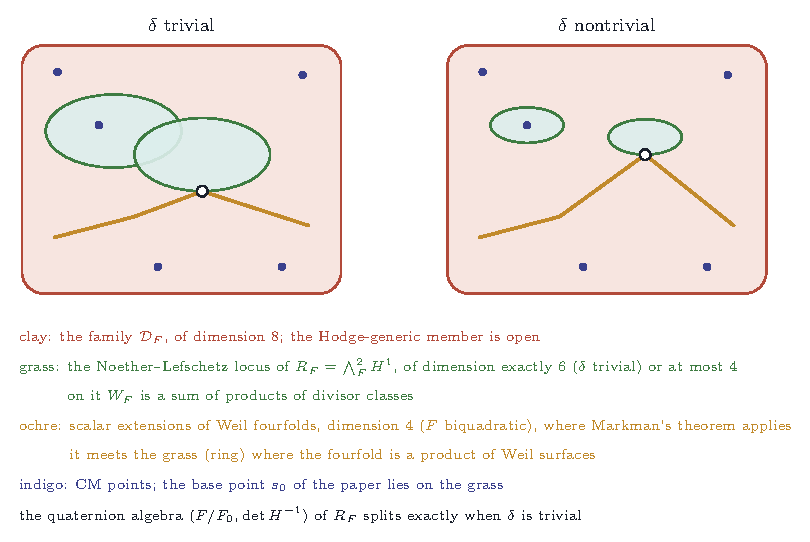
\includegraphics[width=0.94\textwidth]{fig_quarticloci}
\caption{Where the Weil classes of an $(F,2,\delta)$-family are known to be
algebraic, $F$ a quartic CM field; each panel is the period domain
$\cD_{F}$, of dimension $8$. The grass regions are components of the
Noether--Lefschetz locus $\mathrm{NL}(R_{F})$, on which $W_{F}$ consists of
polynomials in divisor classes (\Cref{prop:quarticnl},
\Cref{cor:quarticbase}): of dimension exactly $6$ when $\delta$ is trivial,
where the quaternion algebra $\cQ_{\delta}$ of \Cref{prop:quarticquat} is
split, and at most $4$ otherwise. The ochre curve is the locus of scalar
extensions of Weil fourfolds, of dimension $4$ when $F$ is biquadratic, on
which Markman's theorem applies (\Cref{prop:quarticscalar}); it is not
contained in $\mathrm{NL}(R_{F})$ but meets it (ring) where the fourfold is a
product of Weil surfaces. The indigo points are CM points; the base point
$s_{0}$ of \cite[Theorem~17.5]{paperI} lies on $\mathrm{NL}(R_{F})$. For
$F=\QQ(\zeta_{5}),\QQ(\zeta_{8}),\QQ(\zeta_{12})$ and trivial $\delta$ the Prym
locus of \Cref{rem:quarticprym}, of dimension at most $6$, is not drawn. On
the rest of the domain, the very general member included, the algebraicity
of the Weil classes is the open propagation statement.}
\label{fig:quarticloci}
\end{figure}

\begin{proposition}[Scalar extension from an imaginary quadratic subfield]
\label{prop:quarticscalar}
Let $F=KF_{0}$ with $K$ imaginary quadratic; these are the biquadratic
quartic CM fields, and the only ones containing an imaginary quadratic field.
Let $C$ be an abelian fourfold of $(K,2,\delta)$-Weil type and
$B_{F}=C\otimes_{\cO_{K}}\cO_{F}$, which is of $(F,2,\iota(\delta))$-Weil type by
\cite[Proposition~2.13(ii)]{paperIII}; write $(V_{C},H_{C})$ for the hermitian space of $C$.
For $f\in F$ let $g_{f}\in\Hom(B_{F},C)\otimes\QQ$ be the element inducing
$v\mapsto v\otimes f$ from $H^{1}(C,\QQ)$ to
$H^{1}(B_{F},\QQ)=H^{1}(C,\QQ)\otimes_{K}F$.
\begin{enumerate}[label=\textup{(\roman*)},leftmargin=2.6em,itemsep=2pt]
\item $W_{F}(B_{F})$ lies in the $\QQ$-span of the classes $g_{f}^{*}w$, $f\in F$,
  $w\in W_{K}(C)$, which has dimension $10$. Hence $W_{F}(B_{F})$ is
  algebraic, by Markman's theorem $\mathbf{W}(K,2,\delta)$ \cite{Mar25a}
  (\cite[Proposition~2.12(ii)]{paperIII}).
\item The members $B_{F}$ form a locus of dimension $4$ in the
  $(F,2,\iota(\delta))$-family. At those with $\Hg(C)=\SU(V_{C},H_{C})$ the
  space $R_{F}$ contains no nonzero Hodge class, so
  this locus is not contained in $\mathrm{NL}(R_{F})$; it meets
  $\mathrm{NL}(R_{F})$, for instance where $C=C_{1}\times C_{2}$ with $C_{1}$,
  $C_{2}$ abelian surfaces of Weil type, and then $B_{F}$ is a product of two
  abelian fourfolds of $(F,1)$-Weil type.
\end{enumerate}
\end{proposition}

\begin{proof}
(i) The map $v\mapsto v\otimes f$ commutes with the complex structures, that of
$B_{F}$ being the one of $C$ tensored with $F$, so $g_{f}$ exists. Over $\CC$,
for each embedding $\kappa$ of $K$ let $V_{\kappa}$ be the $\kappa$-eigenspace
of $K$ on $H^{1}(C,\CC)$ and $U_{\kappa}=F\otimes_{K,\kappa}\CC\cong\CC^{2}$, the
sum of the lines $L_{\sigma}$, $\sigma|\kappa$, on which $F$ acts through
$\sigma$. The $\kappa$-part of $H^{1}(B_{F},\CC)$ is $V_{\kappa}\otimes
U_{\kappa}$ and its $\sigma$-part is $V_{\kappa}\otimes L_{\sigma}$, so the
$\sigma$-component $\bigwedge^{4}V_{\kappa}\otimes L_{\sigma}^{\otimes4}$ of
$W_{F}(B_{F})\otimes\CC$ lies in $\bigwedge^{4}V_{\kappa}\otimes
\mathrm{Sym}^{4}U_{\kappa}\subseteq\bigwedge^{4}(V_{\kappa}\otimes U_{\kappa})$.
The map $g_{f}^{*}$ sends a generator $\alpha_{\kappa}$ of $\bigwedge^{4}V_{\kappa}$
to $\alpha_{\kappa}\otimes f_{\kappa}^{\otimes4}$, with $f_{\kappa}$ the image
of $f$ in $U_{\kappa}$. The fourth powers of the elements of the Zariski
dense subset $F$ of $U_{\kappa}$ span $\mathrm{Sym}^{4}U_{\kappa}$, so the
complexified span of the $g_{f}^{*}w$ is $\bigoplus_{\kappa}\bigwedge^{4}V_{\kappa}
\otimes\mathrm{Sym}^{4}U_{\kappa}$, of dimension $2\cdot5$, and it contains
$W_{F}(B_{F})\otimes\CC$. A rational subspace whose complexification lies in
that of a rational subspace lies in it, and pull-backs of algebraic classes
are algebraic.

(ii) The map $C\mapsto B_{F}$ embeds the four-dimensional domain of the
$K$-family into $\cD_{F}$. As rational Hodge structures
$H^{1}(B_{F},\QQ)\cong H^{1}(C,\QQ)^{2}$, so $\Hg(B_{F})=\Hg(C)$, and
$R_{F}\otimes\CC=\bigoplus_{\sigma}\bigwedge^{2}V_{\kappa}\otimes
L_{\sigma}^{\otimes2}$, with $\bigwedge^{2}V_{\kappa}$ irreducible and
nontrivial for $\SL(V_{\kappa})$; so when $\Hg(C)=\SU(V_{C},H_{C})$, $R_{F}$
has no invariants. For $C=C_{1}\times C_{2}$ one has
$B_{F}=(C_{1}\otimes_{\cO_{K}}\cO_{F})\times(C_{2}\otimes_{\cO_{K}}\cO_{F})$, and
\Cref{prop:quarticnl}(iii) applies.
\end{proof}

\Cref{prop:quarticscalar} gives no new case of the Hodge conjecture: $B_{F}$ is
isogenous to $C\times C$, the classes are Hodge classes there, and when
$\Hg(C)=\SU(V_{C},H_{C})$ \cite[Proposition~2.24]{paperIII} already gives the conjecture for
$C\times C$ from \cite{Mar25a}.

\begin{remark}[Prym varieties of cyclic covers]\label{rem:quarticprym}
For three cyclotomic fields published work gives a further locus, at whose
very general points the Hodge group is the whole of $G_{F}$. Let $N\ge3$,
let $\widetilde C\to C$ be an \'etale cyclic cover of degree $N$ of a smooth
projective curve of genus
$g\ge2$, and let $P\subseteq J(\widetilde C)$ be the abelian subvariety on
whose $H^{1}$ the covering group acts through characters of exact order $N$.
Then $F=\QQ(\zeta_{N})$ acts on $P$, and every embedding of $F$ occurs in
$H^{1,0}(P)$ with multiplicity $g-1$ \cite[Lemma~1.6a]{Sch88},
\cite[Lemma~5.1]{PZ25}, so $P$ is of $(F,g-1)$-Weil type
(\cite[Remark~17.2]{paperI}). The hermitian form is split, because the part of
$H_{1}(\widetilde C,\ZZ)$ on which the covering group acts through
characters of exact order $N$ has a hyperbolic $\ZZ[\zeta_{N}]$-basis
\cite[Proposition~2.2]{Loo97}; so $\delta=[(-1)^{g-1}]$, which is trivial for
$g=3$. Schoen proved that the Weil classes of $P$ are algebraic
\cite[Theorem~2.0 with $r=0$, Corollary~3.1]{Sch88}, and Patel and Zhang give
a proof by unramified geometric class field theory
\cite[Theorems~1.1, 1.2 and~5.3, Remark~3.7]{PZ25}. By
\cite[Theorem~2.4]{Loo97}, for every $g\ge2$, the monodromy group of the
family of the $P$ over a finite cover of the moduli of such covers contains a
subgroup of finite index of an arithmetic subgroup of $G_{F}$. Every factor
$\SU(g-1,g-1)$ of $G_{F}(\RR)$ is noncompact, so by Borel's density theorem
\cite{Bor60} its Zariski closure contains $G_{F}$; the Hodge group of every
member lies in $G_{F}$, so by Andr\'e's theorem \cite[Theorem~1]{And92} a very
general $P$ has $\Hg(P)=G_{F}$, and by \cite[Proposition~17.3(iii)]{paperI} the Hodge
conjecture holds for it in every degree. All of this is a consequence of
\cite{Sch88,Loo97,And92}, and we make no claim of priority.

For $\varphi(N)=4$, that is for $F=\QQ(\zeta_{5})=\QQ(\zeta_{10})$,
$\QQ(\zeta_{8})$ and $\QQ(\zeta_{12})$, and $g=3$, the $P$ are abelian
eightfolds of $(F,2,1)$-Weil type. With their $G_{F}(\QQ)$-translates, which
lie in $\Sigma_{F}$ by \cite[Theorem~17.7(ii)]{paperI}, they fill a countable
union of analytic subvarieties of $\cD_{F}$, the \emph{Prym locus} of $F$, of
positive dimension, since the monodromy is infinite, and of dimension at most
$3g-3=6$ \cite[pp.~25--26]{Sch88}. At a very general point of it $\Hg=G_{F}$, so
$R_{F}$ has no nonzero Hodge class there, each $\bigwedge^{2}V_{\sigma}$ being
a nontrivial irreducible representation of $\SL(V_{\sigma})$, and the Hodge
group is larger than that of a scalar extension of a Weil fourfold: such
points lie outside $\mathrm{NL}(R_{F})$, outside the locus of
\Cref{prop:quarticscalar}, and are not CM points. They are the only members
with $\Hg=G_{F}$ at which we know the Weil classes of a quartic CM field to be
algebraic. They do not decide $\mathbf{W}(F,2,1)$: the count
$3g-3=6<8=\tfrac12\varphi(N)(g-1)^{2}=\dim\cD_{F}$ of \cite[pp.~25--26]{Sch88}
makes the union meagre, as $\mathrm{NL}(R_{F})$ is, and
\cite[Theorem~17.7(iii)]{paperI} allows $\Sigma_{F}$ to be meagre. Nor does
\Cref{prop:quarticnogo} exclude them: the cycles come from $J(\widetilde C)$,
which has $P$ as a factor. For imaginary quadratic fields the count is
$3n\ge n^{2}$ for $n\le3$, and there the Prym varieties do reach whole
families: Schoen proved the algebraicity for the Weil fourfolds and for a
family of Weil sixfolds of $\QQ(\sqrt{-3})$ \cite[Theorem~3.2]{Sch88},
\cite{Sch98}, and Koike for a family of Weil sixfolds of $\QQ(\sqrt{-1})$
\cite[Theorem~2.1, Corollary~2.1]{Koi04}.
\end{remark}

\begin{proposition}[The Casimir class]\label{prop:quarticcasimir}
Let $A$ be a member of an $(F,2,\delta)$-family and $c\in F^{\times}$, and let
\[
  C_{q}\in R_{F}\otimes_{\QQ}R_{F}\subseteq H^{2}(A,\QQ)\otimes H^{2}(A,\QQ)
  \subseteq H^{4}(A\times A,\QQ)
\]
be the Casimir element $\sum_{j}u_{j}\otimes u_{j}^{*}$ of the nondegenerate
symmetric form $\Tr_{F/\QQ}(c^{-1}q)$ on $R_{F}$, for a basis $(u_{j})$ and its
dual basis $(u_{j}^{*})$. Then $C_{q}$ is a Hodge class,
$\Delta^{*}C_{q}=6c\,\Omega$ for the diagonal $\Delta\colon A\to A\times A$,
and $C_{q}$ lies in the $\QQ$-span of the classes $f^{*}w$, $w\in W_{F}(A)$,
$f(x,y)=\iota(a)x+\iota(b)y$ with $a,b\in\cO_{F}$. Hence $W_{F}(A)$ is
algebraic if and only if $C_{q}$ is.
\end{proposition}

\begin{proof}
For an $F$-basis $(x_{I})$ of $R_{F}$ and its $q$-dual basis $(x_{I}^{q})$, the
elements $\omega_{k}x_{I}$ and $c\,\omega_{k}^{*}x_{I}^{q}$ form dual bases for
$\Tr_{F/\QQ}(c^{-1}q)$. So by \eqref{eq:quarticstar}
$\Delta^{*}C_{q}=\sum_{I}x_{I}\star(c\,x_{I}^{q})=\sum_{I}c\,\Omega=6c\,\Omega$,
and if $C_{q}$ is algebraic so is $W_{F}(A)$, by \cite[Proposition~17.3(ii)]{paperI}.
Conversely, $\SU(V,H)$ preserves $q$, so $C_{q}$ is invariant under the
diagonal action of $G_{F}$, which contains $\Hg(A\times A)$, and $C_{q}$ is a
Hodge class. Since $q$ pairs $\bigwedge^{2}V_{\sigma}$ only with itself, the
complexification of $C_{q}$ lies in $\bigoplus_{\sigma}\bigwedge^{2}V_{\sigma}
\otimes\bigwedge^{2}V_{\sigma}$, inside the part
$\bigoplus_{\sigma}\bigwedge^{4}(V_{\sigma}\otimes\CC^{2})$ of
$H^{4}(A\times A,\CC)$ on which $F^{\times}$, acting diagonally, has the
characters $\sigma^{4}$. The group $G_{F}$ acts on $V_{\sigma}$ through
$\SL(V_{\sigma})$, whose invariants in $\bigwedge^{4}(V_{\sigma}\otimes\CC^{2})$
are $\bigwedge^{4}V_{\sigma}\otimes\mathrm{Sym}^{4}\CC^{2}$ by Cauchy's
formula, so the $G_{F}$-invariants in that part form the rational space
$W_{F}(A)\otimes_{F}\mathrm{Sym}^{4}_{F}(F^{2})$, of dimension $20$. The map
$f^{*}$ sends $w$ to $w\otimes(a,b)^{\otimes4}$, and the fourth powers of the
elements of $\cO_{F}^{2}$ span $\mathrm{Sym}^{4}_{F}(F^{2})$; so the classes
$f^{*}w$ span that space, and $C_{q}$ is algebraic if $W_{F}(A)$ is.
\end{proof}

\begin{remark}[What the exceptional isogeny gives]\label{rem:quarticisogeny}
By the proof of \Cref{prop:quarticnl}(ii), at each real place $R_{F}$ becomes
$W_{\tau}\otimes\CC$ with $W_{\tau}$ of K3 type, $\SU(V_{\tau},H_{\tau})$ acting
through $\SU(2,2)\to\mathrm{SO}(2,4)$, and when $\delta$ is trivial the
$W_{\tau}$ are the real components of the rational structure $W$ of
\Cref{prop:quarticquat}(iv). A route of Kuga--Satake type would start from
this weight two structure and would have to return to degree four, on $A$ or
on $A\times A$; by \Cref{prop:quarticcasimir} the natural class it meets
there, the Casimir class of $q$, is algebraic exactly when the Weil classes
are. So this mechanism restates $\mathbf{W}(F,2,\delta)$ at each member and
does not reduce it.
\end{remark}

\begin{proposition}[No correspondence from a small abelian variety]
\label{prop:quarticnogo}
Let $A$ be a member with $\Hg(A)=G_{F}$, and let $X$ be an abelian variety
such that $\Hg(X)$ has no normal subgroup isogenous to $G_{F}$; by the proof,
this holds when every simple factor of $X$ has dimension at most $7$, in
particular when $\dim X\le7$, and it holds when $X$ is of CM type. Then
$\Hg(A\times X)=\Hg(A)\times\Hg(X)$, and
$\Hdg^{*}(A^{a}\times X^{b})=\Hdg^{*}(A^{a})\otimes\Hdg^{*}(X^{b})$ for all
$a,b\ge0$. So the class of an algebraic cycle $Z$ on $A^{a}\times X^{b}$ is
$\sum_{i}\beta_{i}\otimes\xi_{i}$ with $\beta_{i}\in\Hdg^{*}(A^{a})$ and
linearly independent $\xi_{i}\in\Hdg^{*}(X^{b})$; the correspondence $Z$
carries $H^{*}(X^{b},\QQ)$ into the span of the $\beta_{i}$; and if the Hodge
conjecture holds for $X^{b}$, every $\beta_{i}$ is algebraic.
\end{proposition}

\begin{proof}
The group $G_{F}=\Res_{F_{0}/\QQ}\SU(V,H)$ is almost simple over $\QQ$. By
Goursat's lemma the kernel $N$ of the projection $\Hg(A\times X)\to\Hg(X)$
maps onto a normal subgroup of $\Hg(A)=G_{F}$. If that subgroup is $G_{F}$,
then $\Hg(A\times X)$ contains $G_{F}\times1$ and is the product. Otherwise
$N$ is finite, $\Hg(X)$ has a normal subgroup $H$ isogenous to $G_{F}$,
contrary to the hypothesis, and the cocharacter $\mu$ defining the Hodge
structure of $X$ projects through $H\to G_{F}$ to that of $A$. This situation
also cannot occur when every simple factor of $X$ has dimension at most $7$,
or when $X$ is of CM type, as follows. Over $\CC$, $H$ is $\SL_{4}\times\SL_{4}$,
and $\mu$ projects in each factor to
$\mathrm{diag}(\frac12,\frac12,-\frac12,-\frac12)$ modulo the centre. Since
$\mu$ acts on $H^{1}(X,\CC)$ with two weights differing by one, the weights of
its projection spread by at most one on every irreducible constituent for
$H$; for the representation of $\SL_{4}$ of highest weight
$a\varpi_{1}+b\varpi_{2}+c\varpi_{3}$ the spread is $a+2b+c$, and spreads add
over the two factors. So every nontrivial constituent is the standard
representation of one factor or its dual. These four are permuted
transitively by $\Gal(\bbar\QQ/\QQ)$, as the embeddings of $F$ are; so a simple
factor $Y$ of $X$ on whose $H^{1}$ the group $H$ acts nontrivially has
$\dim_{\QQ}H^{1}(Y,\QQ)\ge16$, that is $\dim Y\ge8$. A torus has no such $H$.
Next, $\Hg(A^{a}\times X^{b})$ is $\Hg(A)\times\Hg(X)$ acting factorwise on
$H^{*}(A^{a})\otimes H^{*}(X^{b})$, and the invariants of a product of groups
in a tensor product of representations of the factors are the tensor product
of the invariants. Finally, the intersection pairing is perfect on
$\Hdg^{*}(X^{b})$, the invariants being orthogonal to the other isotypic
parts, so there are $\xi_{j}^{*}\in\Hdg^{*}(X^{b})$ with
$\int\xi_{i}\xi_{j}^{*}=\delta_{ij}$; they are algebraic when the conjecture
holds for $X^{b}$, and then $\beta_{j}=pr_{A^{a}*}(Z\cdot pr_{X^{b}}^{*}\xi_{j}^{*})$
is algebraic.
\end{proof}

So a correspondence with such an $X$ can produce a Weil class of $A$ only from
an algebraic cycle on some $A^{a}\times X^{b}$ that already yields one on
$A^{a}$. At a member with full Hodge group this excludes every abelian
variety of dimension at most seven, among them the fourfolds and sixfolds of
Weil type of the imaginary quadratic fields on which Markman's theorems are
proved, and every CM abelian variety. The same argument, with real points in
place of dimensions, excludes rational Hodge structures $Y$ of K3 type: by
Zarhin's theorem \cite{Zar83} the Hodge group of such a $Y$ is the restriction
of scalars of an orthogonal or unitary group over the endomorphism field of
its transcendental part, noncompact at exactly one real place, so its real Lie
algebra has at most one simple factor isomorphic to $\mathfrak{su}(2,2)$,
while that of $G_{F}$ has two; hence $\Hg(A\times Y)=\Hg(A)\times\Hg(Y)$.
This last statement rests on Zarhin's theorem, which we quote without proof.

\begin{theorem}[The polarised criterion for a quartic field at $n=2$]
\label{thm:quarticp2prime}
Let $A$ be a member of an $(F,2,\delta)$-family, let
$\omega=\sum_{\sigma}u_{\sigma}\alpha_{\sigma}$, with $\alpha_{\sigma}$ spanning
$\bigwedge^{4}V_{\sigma}$ and every $u_{\sigma}\ne0$, as holds for every
nonzero rational Weil class, let $p\in\CC[\theta_{1},\theta_{2}]$, put
$\gamma=\omega+p$, and let $r(\gamma)$ be the rank of the contraction
$HT^{2}(A)\to H^{*}(A,\CC)$, $\xi\mapsto\xi\lrcorner\gamma$. Write
$T_{\sigma}=(V_{\sigma}^{1,0})^{\vee}\subseteq T_{0}A$.
\begin{enumerate}[label=\textup{(\roman*)},leftmargin=2.6em,itemsep=2pt]
\item $\dim HT^{2}(A)=28+64+28=120$, and
  \[
    \Ann_{HT^{2}}(\omega)=\textstyle\bigoplus_{\sigma}
    \Hom\bigl(V_{\sigma}^{1,0},V_{\sigma}^{0,1}\bigr)\;\oplus\;
    \bigoplus_{\{\sigma,\sigma'\},\,\sigma\ne\sigma'}T_{\sigma}\otimes T_{\sigma'},
  \]
  of dimension $0+16+24$: the $F$-linear first order deformations of $A$ and
  the bivectors mixing two embeddings. So $r(\omega)=80$. Unlike the case
  $m=1$ of \Cref{thm:p2forces}(i), no nonzero element of $H^{0,2}(A)$ kills
  $\omega$.
\item $r(\gamma)\le112$ for every $p$. For a general $p$, $r(\gamma)=112$, and
  whenever $r(\gamma)=112$ the annihilator of $\gamma$ is the tangent space
  $T_{[A]}\cD_{F}$ of the family, of dimension $8$, inside $H^{1}(T_{A})$. The
  value $112$ is also taken at a general element, with nonzero component in
  $W_{F}\otimes\CC$, of the complexified Hodge ring of a member with
  $\Hg(A)=G_{F}$.
\item $r(\gamma)\ge80$ for every $p$, with equality exactly when $p$ is a
  constant.
\item The rank $r(\gamma)$ takes exactly the fifteen values $80$, $84$, $87$,
  $88$, $91$, $92$, $94$, $95$, $96$, $104$, $107$, $108$, $110$, $111$,
  $112$; \Cref{thm:quarticrank} computes it for every $p$. On the monomials
  $\theta_{1}^{i}\theta_{2}^{j}$ with a general coefficient it takes the
  six values $80$, $84$, $88$, $104$, $108$, $112$.
\item Let $E$ be a perfect complex on $A$ with $\ch(E)=N\omega_{1}+P$, where
  $N\ne0$, $\omega_{1}$ is a nonzero rational Weil class and $P$ is a
  polynomial with rational coefficients in the classes $\eta_{t}$. Then
  $\dim\Ext^{2}(E,E)\ge r(\ch E)\ge80$. If $\dim\Ext^{2}(E,E)=r(\ch E)$, then
  $\operatorname{ev}_{E}$ is onto with kernel $\Ann_{HT^{2}}(\ch E)$ and
  $\sigma_{E}$ is injective, so that $\mathbf{W}(F,2,\delta)$ follows by
  \cite[Theorem~17.7(v)]{paperI}.
\end{enumerate}
\end{theorem}

\begin{proof}
(i) $HT^{2}(A)=\bigwedge^{2}H^{0,1}\oplus H^{0,1}\otimes T_{0}A\oplus
\bigwedge^{2}T_{0}A$, with $H^{0,1}$ and $T_{0}A$ of dimension $8$. As in the
proof of \Cref{thm:p2forces}(i) the three summands map into different Hodge
components, so the annihilator is the sum of the three annihilators; and the
torus $(\CC^{\times})^{4}$ acting on each $V_{\sigma}$ by scalars separates the
images further. A block $V_{\rho}^{0,1}\wedge V_{\rho'}^{0,1}$ of
$\bigwedge^{2}H^{0,1}$ kills $\alpha_{\sigma}$ exactly when
$\sigma\in\{\rho,\rho'\}$, and otherwise maps injectively into a weight space
that no other pair of a block and an embedding reaches; there are four
embeddings, so some $\sigma$ lies outside $\{\rho,\rho'\}$, and no nonzero
element of $\bigwedge^{2}H^{0,1}$ kills $\omega$. A block
$\Hom(V_{\rho}^{1,0},V_{\rho'}^{0,1})$ of $H^{1}(T_{A})$ kills $\alpha_{\sigma}$
for $\sigma\ne\rho$; it kills $\alpha_{\rho}$ when $\rho'=\rho$, because
$V_{\rho}^{0,1}$ is already exhausted in $\alpha_{\rho}$, and maps it
injectively into its own weight space when $\rho'\ne\rho$. A bivector in
$T_{\rho}\otimes T_{\rho'}$ with $\rho\ne\rho'$ kills every $\alpha_{\sigma}$,
whose two factors of type $(1,0)$ both lie in $V_{\sigma}^{1,0}$, and
$\bigwedge^{2}T_{\sigma}$ maps $\alpha_{\sigma}$ to a nonzero multiple of a
generator of $\bigwedge^{2}V_{\sigma}^{0,1}$. The dimensions are $0$,
$4\cdot4$ and $6\cdot4$.

(ii) The classes $\theta_{j}$ and the rational Weil classes stay of Hodge type
along $\cD_{F}$, so each is killed by $T_{[A]}\cD_{F}\subseteq H^{1}(T_{A})$, as
in \Cref{prop:p2primelocus}(i); hence $r(\gamma)\le120-8$, and when equality
holds the annihilator, of dimension $8$, is $T_{[A]}\cD_{F}$. Take a basis of
$H^{1}(A,\CC)$ adapted to the $V_{\sigma}$ and to the Hodge decomposition, in
which the polarisation pairs the basis of $V_{\sigma}^{1,0}$ with that of
$V_{\bbar\sigma}^{0,1}$. The torus acting diagonally on it contains a subtorus
that multiplies each $\theta_{j}$ by a scalar and each $\alpha_{\sigma}$ by an
arbitrary scalar, and contraction is equivariant; so $r(\omega+p)$ depends on
$\omega$ only through a rescaling of the variables of $p$, and each statement
of the theorem holds for every $\omega$ once it holds for one. The rank is
lower semicontinuous in $p$, and it equals $112$ at
$p=\theta_{1}^{2}\theta_{2}^{2}$ by \Cref{thm:quarticrank}(iii) below, so it
equals $112$ for a general $p$. Every element of the complexified Hodge ring
of a member with $\Hg(A)=G_{F}$ is invariant under $G_{F}$, so its components
stay of Hodge type along $\cD_{F}$ and it is killed by $T_{[A]}\cD_{F}$; its
rank is therefore at most $112$. The ring contains $\omega+\theta_{1}^{2}
\theta_{2}^{2}$, since it contains $W_{F}\otimes\CC$ and the classes
$\theta_{1}$, $\theta_{2}$, whose span is defined over $\QQ$, and the rank
is lower semicontinuous; so it is $112$ at a general element of the ring, whose
component in $W_{F}\otimes\CC$ is not zero.

(iii) and (iv) are \Cref{thm:quarticrank}(iii) and (iv) below.

(v) By the commutative square $\sigma_{E}\circ\operatorname{ev}_{E}=(\,\cdot\,)
\lrcorner\ch(E)$ of \Cref{setup:criterion}, which holds on every abelian
variety, $\dim\Ext^{2}(E,E)\ge\operatorname{rk}\operatorname{ev}_{E}\ge
r(\ch E)$, and equality forces $\operatorname{ev}_{E}$ to be onto with kernel
the annihilator and $\sigma_{E}$ to be injective, as in
\Cref{thm:p2primenumber}(iv); and $r(\ch E)\ge80$ by (iii), since the
complexification of $\ch(E)$ is a $\gamma$ as above with $\omega=N\omega_{1}$.
The last implication is \cite[Theorem~17.7(v)]{paperI}, whose character is
exactly of this form.
\end{proof}

At $m=1$ and $n=2$ the corresponding numbers are $28$, $12$ and $24$
(\Cref{thm:p2primenumber}); in both cases the general value is the dimension
of $HT^{2}$ minus that of the family. For the pure shape the argument of
\Cref{thm:p2forces}(ii) and (iv) transfers with the annihilator of
\Cref{thm:quarticp2prime}(i): an injective $\sigma_{E}$ would force
$A_{\theta}A_{\theta'}=0$ for $\theta\in T_{\rho}$, $\theta'\in T_{\rho'}$,
$\rho\ne\rho'$, and a smooth component of the support of codimension at least
two along which $E$ is locally free of positive rank would be tangent to three
of the four $T_{\rho}$. The pure shape is excluded, for every CM
field, by \Cref{thm:cmpurefalse}.

The rank $r(\gamma)$ can be computed for every $p$. In the basis of the
proof of \Cref{thm:quarticp2prime}(ii) write $x_{\sigma,1},x_{\sigma,2}$ for
the basis of $V_{\sigma}^{1,0}$, $y_{\sigma,1},y_{\sigma,2}$ for that of
$V_{\sigma}^{0,1}$, and $\partial_{\sigma,1},\partial_{\sigma,2}$ for the dual
basis of $T_{\sigma}$, so that $\theta_{j}=\sum_{\sigma|\tau_{j}}\sum_{k}
x_{\sigma,k}\,y_{\bbar\sigma,k}$ and $\alpha_{\sigma}=x_{\sigma,1}x_{\sigma,2}
y_{\sigma,1}y_{\sigma,2}$, and use the torus of that proof to make every
$u_{\sigma}$ equal to $1$. Expand
$p=\sum_{i,j=0}^{4}e_{ij}\,\theta_{1}^{i}\theta_{2}^{j}/(i!\,j!)$, so that
$e_{ij}$ is a derivative of $p$ at $0$, and put:
\begin{itemize}[leftmargin=1.6em,itemsep=1pt]
\item $\mu(p)=0$ if $\partial_{1}\partial_{2}p=0$ and $\mu(p)=1$ otherwise,
  the derivatives taken in $\CC[\theta_{1},\theta_{2}]$;
\item $\rho_{1}(p)$ the dimension of the span of $\partial_{1}p$ and
  $\partial_{1}^{2}p$ modulo $\theta_{1}^{3}$, which is the rank of the
  $2\times15$ matrix whose columns are the pairs $(e_{i,j},e_{i+1,j})$,
  $1\le i\le3$, $0\le j\le4$; and $\rho_{2}(p)$ likewise, with the two indices
  exchanged;
\item for $t=1,2$, with $\sigma,\bbar\sigma$ the embeddings over $\tau_{t}$,
  $W_{t}\subseteq HT^{2}(A)$ the span of the eight elements
  $y_{\sigma,1}\wedge y_{\sigma,2}$, $y_{\bbar\sigma,1}\wedge
  y_{\bbar\sigma,2}$, $\partial_{\sigma,1}\wedge\partial_{\sigma,2}$,
  $\partial_{\bbar\sigma,1}\wedge\partial_{\bbar\sigma,2}$ and
  $y_{\sigma,k}\otimes\partial_{\bbar\sigma,l}$,
  $y_{\bbar\sigma,k}\otimes\partial_{\sigma,l}$ with $k\ne l$, and $R_{t}(p)$
  the rank of $\xi\mapsto\xi\lrcorner\gamma$ on $W_{t}$;
\item $h_{1}=e_{1}e_{3}-e_{2}^{2}$, $h_{2}=e_{2}e_{4}-e_{3}^{2}$,
  $h_{3}=e_{1}e_{4}-e_{2}e_{3}$ on $\CC^{4}$, and $V_{\pm}\subset\CC^{4}$ the
  set where $h_{3}=\pm e_{3}$, $2h_{2}=\pm e_{4}$ and $2h_{1}+1=\pm e_{2}$.
\end{itemize}

\begin{theorem}[The rank of the criterion at a quartic field]
\label{thm:quarticrank}
In this notation:
\begin{enumerate}[label=\textup{(\roman*)},leftmargin=2.6em,itemsep=2pt]
\item $r(\gamma)=64+16\mu(p)+4\rho_{1}(p)+4\rho_{2}(p)+R_{1}(p)+R_{2}(p)$.
\item $R_{t}(p)\in\{7,8\}$. If $R_{1}(p)=7$, then
  $(e_{10},e_{20},e_{30},e_{40})$ lies on $V_{+}\cup V_{-}$ and
  $\rho_{1}(p)=2$; conversely, if $\mu(p)=0$ and
  $(e_{10},\dots,e_{40})$ lies on $V_{+}\cup V_{-}$, then $R_{1}(p)=7$, as for
  $p=\theta_{1}^{2}/2$. The same holds for $R_{2}$ with
  $(e_{01},\dots,e_{04})$. Each $V_{\pm}$ contains the surface of points
  $(w\lambda\pm\frac{3}{2\lambda},\,w\lambda^{2}\pm\frac12,\,w\lambda^{3},
  \,w\lambda^{4})$, $w\in\CC$, $\lambda\in\CC^{\times}$.
\item $r(\gamma)\ge80$, with equality exactly when $p$ is a constant, and
  $r(\gamma)$ takes exactly the fifteen values
  \[
    80,\ 84,\ 87,\ 88,\ 91,\ 92,\ 94,\ 95,\ 96,\ 104,\ 107,\ 108,\ 110,\ 111,\
    112 ,
  \]
  the values $87$, $91$, $94$, $95$, $107$, $110$ and $111$ only when $R_{1}$
  or $R_{2}$ is $7$. The value $100$ is not taken.
\item For $\omega=\sum_{\sigma}u_{\sigma}\alpha_{\sigma}$ with arbitrary
  nonzero $u_{\sigma}$, the same holds with $e_{ij}$ replaced by
  $\kappa_{1}^{i}\kappa_{2}^{j}e_{ij}$, where $\kappa_{t}^{4}=
  (u_{\sigma}u_{\bbar\sigma})^{-1}$ for the embeddings over $\tau_{t}$. The
  four choices of $\kappa_{t}$ fix $V_{+}\cup V_{-}$, and $\mu$, $\rho_{1}$,
  $\rho_{2}$ do not depend on them.
\end{enumerate}
\end{theorem}

\begin{proof}
(i) Let $S$ be the torus of the basis that fixes $\theta_{1}$, $\theta_{2}$
and every $\alpha_{\sigma}$. If $x_{\sigma,k}$ has weight $a_{\sigma,k}$, then
$y_{\sigma,k}$ has weight $-a_{\bbar\sigma,k}$ and $\partial_{\sigma,k}$ has
weight $-a_{\sigma,k}$, and the only relations are
$a_{\sigma,1}+a_{\sigma,2}=a_{\bbar\sigma,1}+a_{\bbar\sigma,2}$, one for each
real place; so $S$ has dimension six. Attach to $y_{\sigma,k}$ the label
$(\bbar\sigma,k)$ and to $\partial_{\sigma,k}$ the label $(\sigma,k)$. A basis
element of $HT^{2}$ is a product of two of these and has weight
$-(a_{P}+a_{Q})$ for its two labels $P,Q$, and two such weights agree exactly
when the pairs of labels coincide or are $\{(\sigma,1),(\sigma,2)\}$ and
$\{(\bbar\sigma,1),(\bbar\sigma,2)\}$. So $HT^{2}$ splits into $34$ weight
spaces: the eight lines spanned by $y_{\sigma,k}\otimes
\partial_{\bbar\sigma,k}$; sixteen spaces of dimension four, one for each
pair of labels over different real places; eight of dimension four, one for
each pair $\{(\sigma,k),(\bbar\sigma,l)\}$ over one place; and $W_{1}$,
$W_{2}$. The class $\gamma$ is invariant under $S$, so contraction carries
each weight space into the same weight of $H^{*}(A,\CC)$, and $r(\gamma)$ is
the sum of the ranks on the $34$ spaces.

Two rules compute these ranks. For a label $P=(\rho,k)$ with $\rho$ over
$\tau_{t}$ put $y_{P}=y_{\bbar\rho,k}$, the element of $H^{0,1}$ that carries
it. Contraction by $\partial_{\rho,k}$ is a derivation that maps $\theta_{t}$ to
$\pm y_{P}$ and the other $\theta_{t'}$ to $0$, so it maps $f(\theta_{1},
\theta_{2})$ to $\pm y_{P}\,(\partial_{t}f)(\theta_{1},\theta_{2})$. Hence a basis
element with labels $P,Q$ carries $p$ to $\pm y_{P}y_{Q}\,(Dp)(\theta_{1},
\theta_{2})$, where $D$ is $1$, $\partial_{t}$ or $\partial_{t}\partial_{t'}$
according as none, one or both labels are carried by elements of $T_{0}A$, and
$t,t'$ are their places. Multiplication by $y_{P}y_{Q}$ removes from
$\theta_{1}$ and $\theta_{2}$ the terms that contain $y_{P}$ or $y_{Q}$, and
the products $\theta_{1}^{a}\theta_{2}^{b}$ of what remains are linearly
independent as long as $a$ and $b$ do not exceed the numbers of remaining
terms. Every monomial of $y_{P}y_{Q}f(\theta_{1},\theta_{2})$ contains, with
each $x_{\sigma,i}$, its partner $y_{\bbar\sigma,i}$. The second rule is that
the images of $\omega$ below contain some $x_{\sigma,i}$ without its partner,
so they are independent of every image of $p$.

A line $y_{\sigma,k}\otimes\partial_{\bbar\sigma,k}$ carries $p$ to
$\pm y_{\sigma,k}^{2}(\cdots)=0$ and $\alpha_{\bbar\sigma}$ to
$\pm y_{\sigma,k}x_{\bbar\sigma,k'}y_{\bbar\sigma,1}y_{\bbar\sigma,2}\ne0$,
$k'\ne k$: rank one. On a space of the second kind, with labels
$P=(\rho,k)$ over $\tau_{1}$ and $Q=(\rho',l)$ over $\tau_{2}$, the four basis
elements are $y_{P}\wedge y_{Q}$, $y_{P}\otimes\partial_{\rho',l}$,
$y_{Q}\otimes\partial_{\rho,k}$ and $\partial_{\rho,k}\wedge\partial_{\rho',l}$.
They carry $\omega$ to $y_{P}y_{Q}(\alpha_{\rho}+\alpha_{\rho'})$,
$y_{P}\,(\partial_{\rho',l}\lrcorner\,\alpha_{\rho'})$,
$y_{Q}\,(\partial_{\rho,k}\lrcorner\,\alpha_{\rho})$ and $0$, the factors $y_{P}$
and $y_{Q}$ killing $\alpha_{\bbar\rho}$ and $\alpha_{\bbar\rho'}$; these
contain $x_{\rho,k'}$ or $x_{\rho',l'}$ with $k'\ne k$, $l'\ne l$, without its
partner, and the first three are independent, having two, one and one such
factors $x$ at different places. The bivector carries $\gamma$ to
$\pm y_{P}y_{Q}(\partial_{1}\partial_{2}p)(\theta_{1},\theta_{2})$, with three
terms left in each $\theta_{t}$, and $\partial_{1}\partial_{2}p$ has degree at
most three in each variable; so this image is zero exactly when
$\partial_{1}\partial_{2}p=0$: rank $3+\mu(p)$. On a space of the third kind,
with labels $P=(\sigma,k)$ and $Q=(\bbar\sigma,l)$ over $\tau_{1}$, the element
$y_{P}\wedge y_{Q}$ carries $\omega$ to $y_{P}y_{Q}(\alpha_{\sigma'}+
\alpha_{\bbar\sigma'})$, $\sigma'$ and $\bbar\sigma'$ the embeddings over
$\tau_{2}$, and the other three elements kill $\omega$: $y_{P}\otimes
\partial_{\bbar\sigma,l}$ and $y_{Q}\otimes\partial_{\sigma,k}$ carry
$\alpha_{\bbar\sigma}$ and $\alpha_{\sigma}$ into multiples of
$y_{\bbar\sigma,k}y_{\bbar\sigma,1}y_{\bbar\sigma,2}=0$ and
$y_{\sigma,l}y_{\sigma,1}y_{\sigma,2}=0$, and the bivector meets no
$\alpha$. They carry $p$ to $\pm y_{P}y_{Q}(\partial_{1}p)$, twice, and to
$\pm y_{P}y_{Q}(\partial_{1}^{2}p)$, with two terms left in $\theta_{1}$ and
four in $\theta_{2}$. So the rank is $1$ plus the dimension of the span of
$\partial_{1}p$ and $\partial_{1}^{2}p$ modulo $\theta_{1}^{3}$; in the basis
$\theta_{1}^{a}\theta_{2}^{j}/(a!\,j!)$, $a\le2$, their coefficient vectors are
$(e_{a+1,j})$ and $(e_{a+2,j})$, and the rank is $1+\rho_{1}(p)$; over
$\tau_{2}$ it is $1+\rho_{2}(p)$. The total is
$8+16(3+\mu)+4(1+\rho_{1})+4(1+\rho_{2})+R_{1}+R_{2}$.

(ii) Over $\tau_{1}$ write $x_{k},X_{k},y_{k},Y_{k}$ for $x_{\sigma,k},
x_{\bbar\sigma,k},y_{\sigma,k},y_{\bbar\sigma,k}$, so that
$\theta_{1}=\sum_{k}(x_{k}Y_{k}+X_{k}y_{k})$, $\alpha_{\sigma}=x_{1}x_{2}y_{1}y_{2}$
and $\alpha_{\bbar\sigma}=X_{1}X_{2}Y_{1}Y_{2}$, and put $c=y_{1}y_{2}$,
$C=Y_{1}Y_{2}$, $a_{k}=x_{k}y_{1}y_{2}Y_{k}$, $A_{k}=X_{k}y_{k}Y_{1}Y_{2}$,
$b=x_{1}x_{2}y_{1}y_{2}Y_{1}Y_{2}$ and $B=X_{1}X_{2}y_{1}y_{2}Y_{1}Y_{2}$. Let
$\alpha'$ be the part of $\omega$ over $\tau_{2}$, so that $\alpha'\theta_{2}=0$,
and put $\langle e_{i}\rangle=\sum_{j}e_{ij}\theta_{2}^{j}/j!$. Since $c$ kills
the terms $X_{k}y_{k}$ of $\theta_{1}$, $c\,\theta_{1}^{i}/i!$ is $c$,
$a_{1}+a_{2}$, $-b$ and $0$ for $i=0$, $1$, $2$ and $i\ge3$, so that
$c\gamma=B+c(\alpha'+\langle e_{0}\rangle)+(a_{1}+a_{2})\langle e_{1}\rangle
-b\langle e_{2}\rangle$; in the same way, with $\partial$ acting as a left
derivation, the other seven basis elements of $W_{1}$ carry $\gamma$ to
\begin{align*}
  C\gamma&=b+C(\alpha'+\langle e_{0}\rangle)+(A_{1}+A_{2})\langle e_{1}\rangle
    -B\langle e_{2}\rangle,\\
  \partial_{\sigma,1}\lrcorner\,\partial_{\sigma,2}\lrcorner\,\gamma&=
    -c+C\langle e_{2}\rangle+(A_{1}+A_{2})\langle e_{3}\rangle-B\langle e_{4}\rangle,\\
  \partial_{\bbar\sigma,1}\lrcorner\,\partial_{\bbar\sigma,2}\lrcorner\,\gamma&=
    -C+c\langle e_{2}\rangle+(a_{1}+a_{2})\langle e_{3}\rangle-b\langle e_{4}\rangle,\\
  \pm y_{k}\,\partial_{\bbar\sigma,k'}\lrcorner\,\gamma&=
    A_{k}+c\langle e_{1}\rangle+(a_{1}+a_{2})\langle e_{2}\rangle-b\langle e_{3}\rangle,\\
  \pm Y_{k}\,\partial_{\sigma,k'}\lrcorner\,\gamma&=
    a_{k}+C\langle e_{1}\rangle+(A_{1}+A_{2})\langle e_{2}\rangle-B\langle e_{3}\rangle,
\end{align*}
where $\{k,k'\}=\{1,2\}$ and the sign is $+$ for $k=1$. The differences of
the last two pairs are $A_{1}-A_{2}$ and $a_{1}-a_{2}$. In a basis containing
$A_{1}-A_{2}$, $a_{1}-a_{2}$, $c\alpha'$ and $C\alpha'$, these four
coordinates form the identity matrix on the two differences and on $c\gamma$,
$C\gamma$, and vanish on the other four images. So $R_{1}$ is $4$ plus the rank of the two
images of the bivectors and of the halves of the sums of the last two pairs,
$\tfrac12(A_{1}+A_{2})+c\langle e_{1}\rangle+(a_{1}+a_{2})\langle e_{2}\rangle
-b\langle e_{3}\rangle$ and $\tfrac12(a_{1}+a_{2})+C\langle e_{1}\rangle+
(A_{1}+A_{2})\langle e_{2}\rangle-B\langle e_{3}\rangle$. In the coordinates
along $c$, $a_{1}+a_{2}$, $b$, $C$, $-(A_{1}+A_{2})$, $B$ times
$\theta_{2}^{j}/j!$, and up to the signs of some columns, the matrix of these
four vectors is $K=\bigl(K^{0}\,\big|\,\mathrm{diag}(H,H)\bigr)$: the columns
with $j=0$ form, with $e_{k}=e_{k0}$,
\[
  K^{0}=\begin{pmatrix}
  e_{1}&e_{2}&-e_{3}&0&-\frac12&0\\
  e_{2}&e_{3}&-e_{4}&-1&0&0\\
  0&\frac12&0&e_{1}&-e_{2}&-e_{3}\\
  -1&0&0&e_{2}&-e_{3}&-e_{4}
  \end{pmatrix},
\]
and those with $j\ge1$ form $\mathrm{diag}(H,H)$, with $H$ the $2\times12$
matrix of the pairs $(e_{i,j},e_{i+1,j})$, $1\le i\le3$, $1\le j\le4$. So
$R_{1}=4+\operatorname{rk}K$. Let
$(a,b,c,d)$ annihilate the columns of $K^{0}$. The first two columns give
$d=ae_{1}+be_{2}$ and $c=-2(ae_{2}+be_{3})$, and the other four then say that
$(a,b)$ is orthogonal to the rows of
\[
  Q=\begin{pmatrix}
  e_{3}&e_{4}\\
  -e_{1}e_{2}&e_{2}^{2}-2e_{1}e_{3}-1\\
  2e_{2}^{2}-e_{1}e_{3}-\frac12&e_{2}e_{3}\\
  e_{1}e_{4}-2e_{2}e_{3}&e_{2}e_{4}-2e_{3}^{2}
  \end{pmatrix},
\]
so $\operatorname{rk}K^{0}=2+\operatorname{rk}Q$. If $Q$ were zero, then
$e_{3}=e_{4}=0$ by its first row, $e_{2}^{2}=\frac14$ by its third, and the
second row would have the entry $-\frac34$. So $\operatorname{rk}K\ge3$ and
$R_{1}\ge7$. If $R_{1}=7$, then $\operatorname{rk}Q=1$, and the $2\times2$
minors of $Q$ vanish exactly on $V_{+}\cup V_{-}$. Indeed, with
$P=2h_{1}+1$ and $m_{ij}$ the minor of rows $i$ and $j$, expanding gives
\begin{gather*}
  m_{12}=e_{2}h_{3}-e_{3}P,\quad 2m_{13}=e_{4}P-2e_{2}h_{2},\quad
  m_{14}=2e_{3}h_{2}-e_{4}h_{3},\\
  2m_{23}=e_{2}^{2}-P^{2},\quad m_{24}=Ph_{3}-e_{2}e_{3},\quad
  2m_{34}=e_{3}^{2}-h_{2}-4h_{1}h_{2}.
\end{gather*}
On $V_{\pm}$, $(P,h_{3},2h_{2})=\pm(e_{2},e_{3},e_{4})$, which makes the first
five vanish, and the last is $e_{3}^{2}-h_{2}-2(\pm e_{2}-1)h_{2}=
e_{3}^{2}+h_{2}-e_{2}e_{4}=0$. Conversely, let all six vanish. If
$e_{2}=e_{3}=e_{4}=0$ then $P=1$ and $m_{23}\ne0$; so
$(P,h_{3},2h_{2})=\lambda(e_{2},e_{3},e_{4})$ for some $\lambda$, by the first
three. If $e_{2}\ne0$, then $m_{23}=0$ gives $\lambda=\pm1$. If $e_{2}=0$, then
$P=0$, so $e_{1}e_{3}=-\frac12$, and $h_{3}=e_{1}e_{4}=\lambda e_{3}$ and
$2h_{2}=-2e_{3}^{2}=\lambda e_{4}$ give $e_{4}=-2\lambda e_{3}^{2}$ and then
$\lambda^{2}=1$. In both cases the point lies on $V_{\lambda}$. If moreover $\rho_{1}(p)\le1$, then
$h_{1}=h_{2}=h_{3}=0$, and the minors of the second and third rows and of the
first and third rows become $(e_{2}^{2}-1)/2$ and, once $e_{2}^{2}=1$,
$e_{4}/2$; so $e_{4}=0$, $e_{3}^{2}=e_{2}e_{4}=0$ and $e_{1}e_{3}=0\ne
e_{2}^{2}$, against $h_{1}=0$. Hence $\rho_{1}(p)=2$. If $\mu(p)=0$, then
$e_{ij}=0$ for $i,j\ge1$, so $H=0$ and $R_{1}=6+\operatorname{rk}Q$, which is
$7$ on $V_{\pm}$; the point $(0,1,0,0)$ of $p=\theta_{1}^{2}/2$ lies on $V_{-}$.
The parametrised points satisfy $h_{1}=\pm\frac12w\lambda^{2}-\frac14$,
$h_{2}=\pm\frac12w\lambda^{4}$ and $h_{3}=\pm w\lambda^{3}$, which are the
equations of $V_{\pm}$. The space $W_{2}$ is the same with the indices
exchanged.

(iii) A nonzero $e_{ij}$ with $i,j\ge1$ enters both Hankel matrices, so
$\mu=1$ forces $\rho_{1},\rho_{2}\ge1$, and by (ii) $R_{t}=7$ forces
$\rho_{t}=2$. The tuples $(\mu,\rho_{1},\rho_{2},R_{1},R_{2})$ allowed by
these two conditions give exactly the fifteen values, and $80$ only for
$(0,0,0,8,8)$; $\rho_{1}=\rho_{2}=0$ means that $e_{ij}=0$ unless $i=j=0$,
that is, $p$ is constant. Each value is taken. For $p=0$, $\theta_{1}$,
$\theta_{1}^{2}$, $\theta_{1}^{2}+\theta_{2}$, $\theta_{1}^{2}+\theta_{2}^{2}$,
$\theta_{1}\theta_{2}$, $\theta_{1}\theta_{2}^{2}$ and
$\theta_{1}^{2}\theta_{2}^{2}$ the points $(e_{10},\dots,e_{40})$ and
$(e_{01},\dots,e_{04})$ are $0$, $(1,0,0,0)$ or $(0,2,0,0)$, which lie on
neither $V_{\pm}$, as $2h_{1}+1$ is $1$, $1$ and $-7$ there; so $R_{1}=R_{2}=8$,
and $(\mu,\rho_{1},\rho_{2})$ is $(0,0,0)$, $(0,1,0)$, $(0,2,0)$, $(0,2,1)$,
$(0,2,2)$, $(1,1,1)$, $(1,1,2)$ and $(1,2,2)$, giving $80$, $84$, $88$, $92$,
$96$, $104$, $108$ and $112$. For $p=\theta_{1}^{2}/2+q$ with $q$ one of $0$,
$\theta_{2}$, $\theta_{2}^{2}$, $\theta_{2}^{2}/2$ the point $(0,1,0,0)$ lies on
$V_{-}$ and $\mu=0$, so $R_{1}=7$, and $R_{2}=7$ exactly for $q=\theta_{2}^{2}/2$;
this gives $87$, $91$, $95$ and $94$. For $p=\theta_{1}^{2}/2+\theta_{1}\theta_{2}
+q$ with $q$ one of $0$, $\theta_{2}^{2}$, $\theta_{2}^{2}/2$, the only nonzero
$e_{ij}$ with $i,j\ge1$ is $e_{11}=1$, so the columns of $\mathrm{diag}(H,H)$
are multiples of $(1,0,0,0)$ and $(0,0,1,0)$; at $e=(0,1,0,0)$ the columns of
$K^{0}$ span the space of $(1,0,0,0)$, $(0,0,1,0)$ and $(0,1,0,-1)$, so
$\operatorname{rk}K=3$ and $R_{1}=7$, and likewise $R_{2}=7$ for
$q=\theta_{2}^{2}/2$. With $\mu=1$ and $(\rho_{1},\rho_{2})=(2,1)$, $(2,2)$,
$(2,2)$ this gives $107$, $111$ and $110$.

(iv) The element of the torus of the proof of \Cref{thm:quarticp2prime}(ii)
that multiplies $x_{\sigma,k}$ by $s_{\sigma}$ and $y_{\sigma,k}$ by
$t_{\sigma}$, with $s_{\sigma}t_{\bbar\sigma}=\kappa_{t}$ for $\sigma$ over
$\tau_{t}$, multiplies $\theta_{t}$ by $\kappa_{t}$ and $\alpha_{\sigma}$ by
$(s_{\sigma}t_{\sigma})^{2}$, and these can be chosen to make every
$u_{\sigma}(s_{\sigma}t_{\sigma})^{2}$ equal to $1$ exactly when
$\kappa_{t}^{4}=(u_{\sigma}u_{\bbar\sigma})^{-1}$. It carries $\omega+p$ to the
normalised class with coefficients $\kappa_{1}^{i}\kappa_{2}^{j}e_{ij}$, and
contraction is equivariant. Replacing $\kappa_{t}$ by $-\kappa_{t}$ changes the
signs of $e_{1}$ and $e_{3}$, which fixes $V_{+}$ and $V_{-}$, and replacing
it by $\sqrt{-1}\,\kappa_{t}$ exchanges them; scaling the columns and the
second row of the Hankel matrices does not change their ranks.
\end{proof}

The count of (i), drawn in \Cref{fig:quarticrank}, is the analogue of the
dimension counts of \Cref{thm:p2primenumber} for a field of degree four: sixty-four of the rank
come from the Weil class alone, the Hankel terms measure how far $p$ is from
an exponential in each variable, and the two eight-dimensional spaces
$W_{t}$ carry the exceptional coefficients, the analogue of the exceptional
ratio of \Cref{rem:p2primeexceptional}. Indeed $\rho_{1}(p)\le1$ exactly when
$(e_{10},\dots,e_{40})$ lies on the cone over the twisted cubic, that is,
when the part of $p$ in $\theta_{1}$ alone is, up to a constant, a multiple
of $e^{\lambda\theta_{1}}-1$, of $\theta_{1}$ or of $\theta_{1}^{4}$.

\begin{figure}[tbp]
\centering
  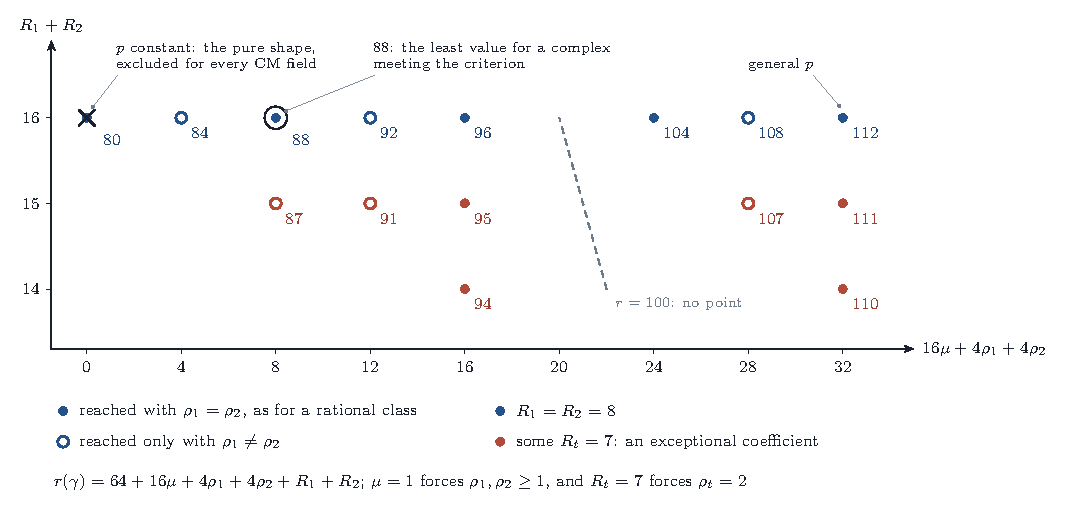
\includegraphics[width=\textwidth]{fig_quarticrank}
\caption{The rank $r(\gamma)$ of \Cref{thm:quarticrank}, over the plane of
the Hankel part $16\mu+4\rho_{1}+4\rho_{2}$ and of $R_{1}+R_{2}$. The fifteen
points are the tuples allowed by the two conditions of the theorem, and each
carries its value. Filled points are reached with $\rho_{1}=\rho_{2}$, as the
character of a complex with rational coefficients is
(\Cref{cor:quarticleast}(ii)); red points need an exceptional coefficient
at one place at least. The value $80$ is the pure shape, excluded for every
CM field by \Cref{thm:cmpurefalse}; so $88$ is the least rank a complex
meeting the criterion can have. The level $r=100$ meets no point.}
\label{fig:quarticrank}
\end{figure}

\begin{corollary}[The least object the criterion asks for]
\label{cor:quarticleast}
Let $E$ be as in \Cref{thm:quarticp2prime}\textup{(v)}.
\begin{enumerate}[label=\textup{(\roman*)},leftmargin=2.6em,itemsep=2pt]
\item $\dim\Ext^{2}(E,E)\ge81$.
\item The coefficients of $P$ satisfy $e_{ji}=\iota(e_{ij})$ for the
  nontrivial automorphism $\iota$ of $F_{0}$, so $\rho_{1}=\rho_{2}$, and
  $r(\ch E)$ is one of $80$, $88$, $94$, $95$, $96$, $104$, $110$, $111$,
  $112$.
\item If $\dim\Ext^{2}(E,E)=r(\ch E)$, then $P$ is not constant and
  $\dim\Ext^{2}(E,E)$ is one of $88$, $94$, $95$, $96$, $104$, $110$, $111$,
  $112$. The value $88$ requires $\mu=0$ and $\rho_{1}=\rho_{2}=1$, and it is
  the rank of $N\omega_{1}+\eta_{s}$ for every $s\in F_{0}^{\times}$.
\end{enumerate}
\end{corollary}

\begin{proof}
(i) By \Cref{thm:quarticp2prime}(v), $\dim\Ext^{2}(E,E)\ge r(\ch E)\ge80$. If
$r(\ch E)=80$, then $P$ is a constant by \Cref{thm:quarticrank}(iii), so
$\ch(E)=c+N\omega_{1}$ and \Cref{thm:cmpurefalse} makes the inequality
strict. (ii) Write $\eta_{t}=\tau_{1}(t)\theta_{1}+\tau_{2}(t)\theta_{2}$
as before \Cref{prop:quarticquat}. A polynomial with rational coefficients in the
$\eta_{t}$ becomes, after exchanging $\theta_{1}$ and $\theta_{2}$, the
polynomial whose coefficients are the images under $\iota$ of the old ones,
so $e_{ji}=\iota(e_{ij})$; the Hankel matrix of $\rho_{2}$ is then the image
under $\iota$ of that of $\rho_{1}$, which has the same rank. The values are
those of \Cref{thm:quarticrank}(iii) with $\rho_{1}=\rho_{2}$, the scaling
of (iv) there changing neither $\mu$ nor the $\rho_{t}$. (iii) If $P$ were
constant, \Cref{thm:cmpurefalse} would give $\dim\Ext^{2}(E,E)>r(\ch E)$.
For $P=\eta_{s}$ the pairs are $(\tau_{t}(s),0)$, so $\rho_{1}=\rho_{2}=1$,
$\mu=0$, and $R_{t}=8$ by \Cref{thm:quarticrank}(ii).
\end{proof}

The Weil tori of \Cref{setup:cmweiltori} exclude more than the pure shape.
A polynomial in $\theta_{1},\theta_{2}$ can stay of Hodge type on all of
$S_{F}$, and then the argument of \Cref{thm:cmpurefalse} applies to it.

\begin{proposition}[The characters that the Weil tori exclude]
\label{prop:quarticweiltori}
Let $E$ be as in \Cref{thm:quarticp2prime}\textup{(v)}, and suppose that $P$
lies in the span of the $\theta_{1}^{i}\theta_{2}^{j}$ with
$i,j\in\{0,4\}$, as for $\ch(E)=c+N\omega_{1}+b\,\theta_{1}^{4}+
\iota(b)\,\theta_{2}^{4}$ with $b\in F_{0}$. Then $\sigma_{E}$ is not
injective and $\dim\Ext^{2}(E,E)>r(\ch E)$. Consequently, if
$\dim\Ext^{2}(E,E)=r(\ch E)=88$, then $P=c+f(\theta_{1})+f^{\iota}(\theta_{2})$
with $c\in\QQ$, where $f(\theta)$ is a nonzero multiple either of $\theta$ or
of $e^{\lambda\theta}-1$ for some $\lambda\ne0$, and $f^{\iota}$ is obtained
by applying $\iota$ to the coefficients of $f$.
\end{proposition}

\begin{proof}
In the basis before \Cref{thm:quarticrank}, $\theta_{1}$ is a sum of four
products of two classes, one from $V_{\sigma}$ and one from $V_{\bbar\sigma}$
for the two embeddings over $\tau_{1}$, in disjoint sets of basis vectors.
So $\theta_{1}^{4}$ is $4!$ times their product, a nonzero element of
$\bigwedge^{4}V_{\sigma}\otimes\bigwedge^{4}V_{\bbar\sigma}$, that is a
nonzero multiple of $\alpha_{\sigma}\alpha_{\bbar\sigma}$, and likewise for
$\theta_{2}^{4}$. Hence $\ch(E)=N\omega_{1}+P$ lies in the span of the
classes $\alpha_{\Sigma}$, which are of type $(p,p)$ on every member of
$S_{F}$ (\Cref{setup:cmweiltori}); being rational, it is a Hodge class on
every member. Its component of degree four is $N\omega_{1}\ne0$, since $P$
has none, and \Cref{thm:cmpurefalse} applies. If $\dim\Ext^{2}(E,E)=
r(\ch E)=88$, then $\mu=0$ and $\rho_{1}=\rho_{2}=1$ by
\Cref{cor:quarticleast}(iii), so $P$ has no mixed monomials, and by the
paragraph after \Cref{thm:quarticrank} its part in $\theta_{1}$ alone is a
multiple of $e^{\lambda\theta_{1}}-1$, of $\theta_{1}$ or of $\theta_{1}^{4}$;
its part in $\theta_{2}$ alone is obtained by $\iota$, by
\Cref{cor:quarticleast}(ii). In the third case $P$ lies in the span of
$1$, $\theta_{1}^{4}$ and $\theta_{2}^{4}$, which the first part excludes.
\end{proof}

The shape $c+b\,\theta_{1}^{4}+\iota(b)\,\theta_{2}^{4}$ has rank $88$, and
with a multiple of $\theta_{1}^{4}\theta_{2}^{4}$ added it has rank $104$,
by \Cref{thm:quarticrank}: $\rho_{1}=\rho_{2}=1$, $\mu$ is $0$ or $1$, and
$R_{1}=R_{2}=8$, since $(e_{10},\dots,e_{40})=(0,0,0,24b)$ with $b\ne0$ does
not meet $V_{+}\cup V_{-}$. \Cref{prop:quarticweiltori} removes
both. What remains at $88$ is a Chern character whose polynomial part is
exponential or linear in each $\theta_{t}$ separately, such as
$c+\eta_{s}+N\omega_{1}$. For these the classes $\theta_{t}$ are not of Hodge
type on the Weil tori, and the argument needs a family of complex tori along
which the character stays of Hodge type and whose members are not algebraic.
The next proposition, the analogue for a quartic field of
\Cref{prop:p2primelocus}(iii) and (iv), shows that there is none: the Hodge
locus of such a character is the polarised family itself.

\begin{proposition}[The Hodge locus of a character at a quartic field]
\label{prop:quarticlocus}
Keep the notation before \Cref{thm:quarticrank}, with $\gamma=\omega+p$ and
every $u_{\sigma}\ne0$, and for the embeddings $\sigma,\bbar\sigma$ over
$\tau_{t}$ put $\omega_{t}=u_{\sigma}\alpha_{\sigma}+u_{\bbar\sigma}
\alpha_{\bbar\sigma}$. Call $\tau_{t}$ a \emph{mid place} of $p$ if $p$ has a
monomial $\theta_{1}^{i}\theta_{2}^{j}$ with nonzero coefficient whose exponent
of $\theta_{t}$ is $1$, $2$ or $3$, and call a mid place \emph{exceptional} if
the only such monomial is $\theta_{t}^{2}$ itself and its coefficient $c_{t}$
in $p$ satisfies $c_{t}^{2}\theta_{t}^{4}=\frac34\,\omega_{t}^{2}$, the ratio
of \Cref{prop:p2primelocus}(iv).
\begin{enumerate}[label=\textup{(\roman*)},leftmargin=2.6em,itemsep=2pt]
\item The annihilator of $\gamma$ in $H^{1}(T_{A})$ is the space of $F$-linear
  $\xi\in\bigoplus_{\sigma}\Hom(V_{\sigma}^{1,0},V_{\sigma}^{0,1})$ with
  $\xi\lrcorner\theta_{t}=0$ at every mid place, plus, at each exceptional
  place, a line spanned by an element of $\Hom(V_{\sigma}^{1,0},
  V_{\bbar\sigma}^{0,1})\oplus\Hom(V_{\bbar\sigma}^{1,0},V_{\sigma}^{0,1})$
  with both components nonzero. Its dimension is $8+4a+b$, where $a$ is the
  number of places that are not mid places and $b$ the number of exceptional
  places.
\item The connected component through $A$ of the Hodge locus of $\gamma$, in
  the space of complex structures on the real torus underlying $A$, is
  $S_{F}$ when neither place is a mid place, that is when $p$ lies in the
  span of the $\theta_{1}^{i}\theta_{2}^{j}$ with $i,j\in\{0,4\}$; and it is
  $\cD_{F}$ when both places are mid places and neither is exceptional. In
  the second case all its members are abelian varieties polarised by
  $\theta_{1}+\theta_{2}$.
\item If both places are exceptional, then near $A$ the Hodge locus is the
  orbit of $A$ under $G_{1}\times G_{2}$, where $G_{t}\cong\mathrm{Spin}(4,3)$
  is the connected stabiliser of $X_{t}=\omega_{t}+c_{t}\theta_{t}^{2}$ in the
  real linear group of $V_{\sigma}\oplus V_{\bbar\sigma}$, and it has
  dimension $10$. A very general member $T$ of it has $\NS(T)=0$ and
  $\Hdg^{2}(T)\otimes\CC$ contained in the span of $X_{1}$ and $X_{2}$, and on
  every member, for every K\"ahler class $\kappa$, $\int X_{t}\,\kappa^{6}$ is
  nonzero with the sign of $c_{t}$, in the normalisation in which
  $\theta_{t}$ is a real class with $\theta_{t}^{2}$ positive.
\item If $\gamma$ is the complexified character of \Cref{thm:quarticp2prime}(v),
  then both places are mid places or neither is, and both are exceptional or
  neither is; and an exceptional $\gamma$ has $r(\gamma)=94$, or $110$ when
  $p$ contains $\theta_{1}^{4}\theta_{2}^{4}$.
\end{enumerate}
\end{proposition}

\begin{proof}
(i) Grade $\bigwedge^{*}H^{1}$ by the degrees in the four $V_{\sigma}$, and
write $\xi_{\sigma\sigma'}$ for the component of $\xi$ in
$\Hom(V_{\sigma'}^{1,0},V_{\sigma}^{0,1})$, which raises the degree in
$V_{\sigma}$ by one and lowers that in $V_{\sigma'}$ by one. The monomial
$\theta_{1}^{i}\theta_{2}^{j}$ has degree $i$ in the two embeddings over
$\tau_{1}$ and $j$ in those over $\tau_{2}$, and $\alpha_{\sigma}$ has degree
$4$ in $V_{\sigma}$. By the proof of \Cref{thm:quarticp2prime}(i),
$\xi_{\sigma\sigma}\lrcorner\omega=0$, and for $\sigma\ne\sigma'$ the only
term of $\xi_{\sigma\sigma'}\lrcorner\omega$ is
$u_{\sigma'}\xi_{\sigma\sigma'}\lrcorner\alpha_{\sigma'}$, of degree $3$ in
$V_{\sigma'}$ and $1$ in $V_{\sigma}$, which determines $\xi_{\sigma\sigma'}$.
A term $\xi_{\rho\rho'}\lrcorner\theta_{1}^{i}\theta_{2}^{j}$ has that degree
only if $\sigma,\sigma'$ lie over the same place $\tau_{t}$, $(i,j)$ is
$(2,0)$ or $(0,2)$ with the $2$ at $t$, and $(\rho,\rho')=(\sigma',\sigma)$.
So every component $\xi_{\sigma\sigma'}$ with $\sigma,\sigma'$ over different
places vanishes, and the equations split into the $F$-linear part and, at
each place, the pair $\xi'=\xi_{\bbar\sigma\sigma}$, $\xi''=\xi_{\sigma\bbar\sigma}$.

For $F$-linear $\xi$ put $D_{t}=\xi\lrcorner\theta_{t}\in V_{\sigma}^{0,1}
\otimes V_{\bbar\sigma}^{0,1}$; the map $\xi\mapsto(D_{1},D_{2})$ is onto, with
kernel $T_{[A]}\cD_{F}$. Then $\xi\lrcorner\theta_{1}^{i}\theta_{2}^{j}
=i\,\theta_{1}^{i-1}\theta_{2}^{j}D_{1}+j\,\theta_{1}^{i}\theta_{2}^{j-1}D_{2}$,
the monomials lie in different degrees, and the two terms have different
Hodge types at the two places, so each vanishes. Now $\theta_{t}^{3}D_{t}=0$
for every $D_{t}$, as a degree count shows, while multiplication by
$\theta_{t}^{k}$ is injective on $V_{\sigma}^{0,1}\otimes V_{\bbar\sigma}^{0,1}$
for $k\le2$: $\theta_{t}^{2}y_{\sigma,k}y_{\bbar\sigma,l}$ is $2$ times the
product of $y_{\sigma,k}y_{\bbar\sigma,l}$ with the two terms of $\theta_{t}$
that avoid $y_{\sigma,k}$ and $y_{\bbar\sigma,l}$, and different $(k,l)$ give
different monomials. Multiplication by $\theta_{t'}^{j}$, $j\le4$, acts on the
other factor of $\bigwedge^{*}H^{1}=\bigwedge^{*}(V_{\sigma}\oplus
V_{\bbar\sigma})\otimes\bigwedge^{*}(V_{\sigma'}\oplus V_{\bbar\sigma'})$ and is
nonzero there. So the conditions on the $F$-linear part are exactly $D_{t}=0$
at the mid places, a space of dimension $16-4(2-a)=8+4a$.

At a place $\tau_{t}$ let $c_{t}$ be the coefficient of $\theta_{t}^{2}$ in $p$.
The terms involving $\xi''$ are $u_{\bbar\sigma}\xi''\lrcorner
\alpha_{\bbar\sigma}+c_{t}\,\xi'\lrcorner\theta_{t}^{2}$, of degree $3$ in
$V_{\bbar\sigma}$ and $1$ in $V_{\sigma}$, the same with $\sigma$ and
$\bbar\sigma$ and with $\xi'$ and $\xi''$ exchanged, and
$i\,\theta_{t}^{i-1}\theta_{t'}^{j}(\xi'\lrcorner\theta_{t})$ and its analogue
for $\xi''$ for every other monomial with exponent $i\in\{1,2,3\}$ of
$\theta_{t}$. Here $\xi'\lrcorner\theta_{t}$ lies in the line
$\bigwedge^{2}V_{\bbar\sigma}^{0,1}$, on which multiplication by
$\theta_{t}^{i-1}\theta_{t'}^{j}$ is injective for $i\le3$ by the same count. If
such another monomial occurs, $\xi'\lrcorner\theta_{t}=\xi''\lrcorner
\theta_{t}=0$, and then $\xi'=\xi''=0$, the maps $\xi'\mapsto
\xi'\lrcorner\alpha_{\sigma}$ and $\xi''\mapsto\xi''\lrcorner\alpha_{\bbar\sigma}$
being injective. Otherwise $\xi''\lrcorner\theta_{t}^{2}=2\theta_{t}\,
(\xi''\lrcorner\theta_{t})$ is a multiple of $\theta_{t}\,y_{\sigma,1}
y_{\sigma,2}$, which is $\xi'_{0}\lrcorner\alpha_{\sigma}$ for one element
$\xi'_{0}$, and likewise with $\sigma$ and $\bbar\sigma$ exchanged; so $\xi'$
and $\xi''$ are multiples of $\xi'_{0}$ and $\xi''_{0}$. Explicitly,
$\xi'_{0}(x_{\sigma,1})=-y_{\bbar\sigma,2}$ and
$\xi'_{0}(x_{\sigma,2})=y_{\bbar\sigma,1}$ give
$\xi'_{0}\lrcorner\alpha_{\sigma}=\theta_{t}\,y_{\sigma,1}y_{\sigma,2}$ and
$\xi'_{0}\lrcorner\theta_{t}=2y_{\bbar\sigma,1}y_{\bbar\sigma,2}$, and
symmetrically for $\xi''_{0}$. Writing $\xi'=a\xi'_{0}$ and
$\xi''=b\xi''_{0}$, the two remaining equations are
$u_{\sigma}a+4c_{t}b=0$ and $4c_{t}a+u_{\bbar\sigma}b=0$, and their
determinant vanishes exactly when $16c_{t}^{2}=u_{\sigma}u_{\bbar\sigma}$. Since $\theta_{t}^{4}=24\,
\alpha_{\sigma}\alpha_{\bbar\sigma}$ and $\omega_{t}^{2}=2u_{\sigma}
u_{\bbar\sigma}\alpha_{\sigma}\alpha_{\bbar\sigma}$, that is the condition
$c_{t}^{2}\theta_{t}^{4}=\frac34\omega_{t}^{2}$, and the solutions then form a
line on which both components are nonzero.

(ii) By \Cref{prop:p2primelocus}(i), applied to each homogeneous component,
the Hodge locus of $\gamma$ in the chart at $A$ is the linear space
$\Ann_{H^{1}(T_{A})}(\gamma)$. If neither place is a mid place, that space is
the space of all $F$-linear $\xi$, which is also the part of $S_{F}$ in the
chart; $\gamma$ is of Hodge type on all of $S_{F}$, as in the proof of
\Cref{prop:quarticweiltori}, and at every member of $S_{F}$ its component of
degree four is $\omega$, whose annihilator in $H^{1}(T)$ is again the space of
$F$-linear deformations (\Cref{thm:quarticp2prime}(i), whose proof uses only
the decomposition into the $V_{\sigma}$). So $S_{F}$ is open in the Hodge locus;
it is closed in the space of complex structures, since commuting with $F$ is a
closed condition and the dimensions of the $H^{1,0}\cap V_{\sigma}$ are
locally constant on it; and it is connected. If both places are mid places
and neither is exceptional, the annihilator is $T_{[A]}\cD_{F}$ by (i), at
every member of $\cD_{F}$, since the conditions of (i) are stated in terms of
the flat classes $\theta_{t}$ and $\omega_{t}$; and the argument of
\Cref{prop:p2primelocus}(iii) shows that $\cD_{F}$ is open, closed and
connected in the Hodge locus.

(iii) At each place $X_{t}$ is, in the $8$-dimensional space
$V_{\sigma}\oplus V_{\bbar\sigma}$ with the form $\theta_{t}$, the class of
\Cref{rem:p2primeexceptional}, and the argument there applies word for
word, with the factor $\mathfrak{su}(2,2)$ at $\tau_{t}$ of the Lie algebra of $G_{F}$
in place of the Hodge group: the stabiliser is $\mathfrak{so}(4,3)$, with an
orbit of dimension $5$ in the Grassmannian. The other components of $\gamma$ are constants, multiples of
$\theta_{t}^{4}$, which is $24$ times the volume form of
$V_{\sigma}\oplus V_{\bbar\sigma}$, and of $\theta_{1}^{4}\theta_{2}^{4}$, all
fixed by $G_{1}\times G_{2}$. So the orbit of $A$ lies in the Hodge locus,
and it has dimension $10$, which by (i) is that of the locus near $A$. A
rational class of Hodge type at a very general member is of Hodge type on the
whole orbit, hence killed by the complex structures of all its members,
which lie in $\mathfrak{g}_{1}\oplus\mathfrak{g}_{2}$ and generate an ideal
projecting nontrivially to both simple factors, that is all of it. The
invariants of $\mathfrak{so}(7,\CC)$ in the exterior algebra of its spin
representation are $1$, $X_{t}$ and the volume form
(\Cref{rem:p2primeexceptional}), so in degree two there are none and in
degree four only $X_{1}$ and $X_{2}$. For the sign, a K\"ahler class is
$\kappa_{h}$ for a positive hermitian form $h$ on the tangent space; only the
terms of $\kappa_{h}^{6}$ that contain the whole volume of the other place pair
with $X_{t}$, and they give $\det(h_{t'})$ times $\kappa_{h'}^{2}$ for the
Schur complement $h'$ of $h_{t'}$ in $h$, a positive hermitian form on the
tangent space at $\tau_{t}$. So $\int X_{t}\kappa_{h}^{6}$ is a positive
multiple of the integral of \Cref{rem:p2primeexceptional} for $h'$, which has
the sign of $c_{t}$; and $G_{1}\times G_{2}$ fixes $X_{t}$ and carries K\"ahler
cones to K\"ahler cones.

(iv) An automorphism of $\bbar\QQ$ inducing $\iota$ on $F_{0}$ fixes the
rational class $\gamma$ and exchanges $\theta_{1}$ with $\theta_{2}$ and
$\omega_{1}$ with $\omega_{2}$, so it carries the conditions at $\tau_{1}$ to
those at $\tau_{2}$. An exceptional $p$ lies in the span of $1$,
$\theta_{t}^{2}$, $\theta_{t}^{4}$ and $\theta_{1}^{4}\theta_{2}^{4}$ with
$c_{t}\ne0$, so $\rho_{1}=\rho_{2}=2$, $\mu=1$ exactly when
$\theta_{1}^{4}\theta_{2}^{4}$ occurs, and $(e_{10},\dots,e_{40})$ lies on
$V_{+}\cup V_{-}$, so $R_{1}=R_{2}=7$ by \Cref{thm:quarticrank}(ii); the
formula of \Cref{thm:quarticrank}(i) gives $94$ or $110$.
\end{proof}

\begin{corollary}[The Weil tori at rank $88$]\label{cor:quarticlocus}
Let $E$ be as in \Cref{thm:quarticp2prime}\textup{(v)} with
$\dim\Ext^{2}(E,E)=r(\ch E)=88$, so that $\ch(E)=N\omega_{1}+c+f(\theta_{1})
+f^{\iota}(\theta_{2})$ as in \Cref{prop:quarticweiltori}. Then the connected
component through $A$ of the Hodge locus of $\ch(E)$ is $\cD_{F}$, and every
complex torus reached from $A$ by a deformation along which $\ch(E)$ stays of
Hodge type is an abelian variety of the family. So no argument that deforms
$E$ itself to a torus that is not algebraic can exclude it; the characters
that such an argument excludes at $88$ are exactly those of
\Cref{prop:quarticweiltori}.
\end{corollary}

\begin{proof}
The coefficient $e_{10}$ of $f$ is nonzero, both for a multiple of $\theta$
and for one of $e^{\lambda\theta}-1$, and $e_{01}=\iota(e_{10})$, so both
places are mid places, with the monomials $\theta_{1}$ and $\theta_{2}$, and
neither is exceptional. \Cref{prop:quarticlocus}(ii) applies.
\end{proof}

As after \Cref{prop:p2primelocus}, this concerns $E$ itself: an
autoequivalence of $D^{b}(A)$ changes the character, and the proposition then
applies to the new one. For the exceptional characters of
\Cref{prop:quarticlocus}(iii), of rank $94$ or $110$, the proof of
\Cref{thm:cmpurefalse} can be started, since the locus contains tori without
divisors, but it breaks down as in \Cref{rem:p2primeexceptional}: the classes
$X_{t}$ have integrals of constant sign against every K\"ahler class, so
Bando and Siu give no vanishing: they bound the signs of the coefficients of
$\ch_{2}$ of a torsion-free sheaf along $X_{1}$ and $X_{2}$, which a complex,
an alternating sum, need not respect. So at a
quartic field the Weil tori and their exceptional analogues exclude exactly
the characters of \Cref{prop:quarticweiltori}, and what the criterion still
asks for, at $88$ and above, is the construction of an object.

The natural candidates are Markman's secant objects \cite{Mar25c}, in the
twisted form in which he states his reduction. For them a $B$-field twist of
$\ch(E)$, the class $\kappa$ of \Cref{thm:quarticobstruction}, is flat, and
under a non-degeneracy condition its component in $H^{4}$ is a polynomial in
the $\eta_{t}$ plus a nonzero Weil class
\cite[Proposition~10.2.1, Theorem~1.1.2]{Mar25c}. But $\ch(E)$ itself is not
flat, and $\kappa$ is not of the form $N\omega+P(\eta)$ in higher degrees
(\Cref{rem:quarticsecantshape}), so they are candidates only for a twisted
form of \Cref{thm:quarticp2prime}(v). The dimension count that works for
imaginary quadratic fields (\Cref{thm:twistedcert}) can be tested on them
exactly. Let $X$ be a principally polarised abelian fourfold with real
multiplication by the ring of integers $\cO_{F_{0}}$, write
$\theta_{1},\theta_{2}\in H^{2}(X,\RR)$ for the components of the
polarisation at the two real places of $F_{0}$, so that
$\theta=\theta_{1}+\theta_{2}$ and $\theta_{j}^{3}=0$, and let $\mathcal{R}$ be
the $\QQ$-subalgebra of $H^{\mathrm{ev}}(X,\QQ)$ spanned by the rational
combinations of the $\theta_{1}^{a}\theta_{2}^{b}$, $0\le a,b\le2$. A class
$v=\sum_{a,b}V_{ab}\,\theta_{1}^{a}\theta_{2}^{b}/(a!\,b!)$ of $\mathcal{R}$ has a
$3\times3$ matrix $V$ with entries in $F_{0}\otimes\RR$.

\begin{proposition}[The secant space of a quartic field]\label{prop:quarticsecant}
Let $F=F_{0}(\sqrt{-q})$ with $q\in F_{0}$ totally positive, let $t\in F_{0}$,
$s_{j}=\sqrt{-1}\,\sqrt{\tau_{j}(q)}$, and for $\varepsilon\in\{\pm1\}^{2}$ put
$e_{\varepsilon}=\exp\bigl(\sum_{j}(\tau_{j}(t)+\varepsilon_{j}s_{j})\theta_{j}\bigr)$.
\begin{enumerate}[label=\textup{(\roman*)},leftmargin=2.6em,itemsep=2pt]
\item The span $S(t,q)$ of the four $e_{\varepsilon}$ is a rational subspace of
  $\mathcal{R}$ of dimension $4=2^{[F_{0}:\QQ]}$, secant to the spinor variety.
  For $t=0$ it is the secant space of \cite[\S11.1, (11.1.2)]{Mar25c} for the
  polarisation $\theta$ and $q$; replacing $\theta$ by $f\theta$,
  $f\in F_{0}^{\times}$, replaces $q$ by $qf^{2}$, and a rational $F_{0}$-$B$-field
  $t$ transports Markman's $F$-structure by the rational automorphism of
  $X\times\widehat X$ acting on $H^{*}(X)$ as $e^{\theta_{t}}$,
  $\theta_{t}=\sum_{j}\tau_{j}(t)\theta_{j}$, and replaces $S(0,q)$ by
  $S(t,q)=e^{\theta_{t}}S(0,q)$.
\item For $v=\sum_{\varepsilon}w_{\varepsilon}e_{\varepsilon}\in S(t,q)$ let
  $\rho=\rk V$ and $N_{w}=\#\{\varepsilon:w_{\varepsilon}\ne0\}$. The ranks of
  contraction from $HT^{k}(X)$ into $v$ are $1$, $8$ and $2\rho+4N_{w}$ for
  $k=0,1,2$, with $(\rho,N_{w})\in\{(1,4),(2,4),(2,2)\}$, and $N_{w}=2$ only for
  biquadratic $F$ and $v$ in the secant plane of one of its two imaginary
  quadratic subfields \cite[\S11.2.1]{Mar25c}.
\item For $v=e^{\theta_{t}}(a\,u+v_{f}+c\,w)$ in the basis
  $u=(1-\tfrac12q_{1}\theta_{1}^{2})(1-\tfrac12q_{2}\theta_{2}^{2})$,
  $v_{f}=\theta_{f}-\tfrac12\theta_{\bar fq}\theta_{1}\theta_{2}$,
  $w=\theta_{1}\theta_{2}$ of $e^{-\theta_{t}}S(t,q)$, one has
  $\chi(v,v)=\int_{X}v^{\vee}v=4\bigl(\Nm(q)a^{2}+c^{2}+\Tr(\bar q f^{2})\bigr)$,
  which is positive definite.
\end{enumerate}
\end{proposition}

\begin{proof}
(i) The Galois group permutes the four exponentials as it permutes the CM
types of $F$, so their span is rational; since $\theta_{j}^{3}=0$,
$e^{\pm s_{j}\theta_{j}}=(1-\tfrac12\tau_{j}(q)\theta_{j}^{2})\pm s_{j}\theta_{j}$, and
the four classes are independent. The conjugates in
$\mathfrak{so}\cap\End^{0}(X\times\widehat X)$ of the standard structure have
eigenvalues $t\pm s$, and the pure spinors of their eigenspaces are the
$e_{\varepsilon}$.

(ii) Over $\CC$, $H^{1}(X)=U_{1}\oplus U_{2}$ with $U_{j}$ the
eigenspaces of $F_{0}$, and $HT^{*}(X)$ and $H^{*}(X)$ are tensor products over
$j$, compatibly with contraction. By \Cref{lem:bfield}(i),
$\xi\lrcorner e^{\lambda\theta_{j}}=y^{\lambda}(\xi)e^{\lambda\theta_{j}}$, and the
blocks $HT_{1}^{a}\otimes HT_{2}^{b}$ have independent images because they
shift the two Hodge bidegrees by $(a,b)$ while $v$ is balanced. The block
$(1,1)$ contributes $4N_{w}$, by the invertibility of the Hadamard matrix of
the signs; the blocks $(2,0)$ and $(0,2)$ contribute $\rho$ each; the blocks
$(1,0)$ and $(0,1)$ contribute $4$ each in degree one. Reality gives
$w_{-\varepsilon}=\overline{w_{\varepsilon}}$, and when $F$ is not biquadratic
the Galois group acts transitively on the CM types, so $N_{w}=4$.

(iii) One has
$\int_{X}e^{c_{1}\theta_{1}+c_{2}\theta_{2}}=c_{1}^{2}c_{2}^{2}$, and $\chi$ is
invariant under $e^{\theta_{t}}$; the form is positive definite because $q$ is
totally positive.
\end{proof}

The integral classes of $\mathcal{R}$ are described by one congruence, and
the description does not depend on the field.

\begin{lemma}[The integral classes of $\mathcal{R}$]\label{lem:quarticlattice}
Let $F_{0}$ be a real quadratic field with ring of integers $\cO$ and
different $\mathfrak d$, and let $X$ be a principally polarised abelian
fourfold with real multiplication by $\cO$. A class $v\in\mathcal{R}$ with
matrix
\[
  V=\begin{pmatrix}r&\bar h&\bar g\\ h&c&\bar k\\ g&k&m\end{pmatrix},
  \qquad r,c,m\in\QQ,\quad h,g,k\in F_{0},
\]
lies in $H^{\mathrm{ev}}(X,\ZZ)$ if and only if $r,c,m\in\ZZ$,
$h,g,k\in\cO$ and $c\equiv g$ modulo $\mathfrak d$.
\end{lemma}

\begin{proof}
Integrality can be tested one prime $p$ at a time, and after a faithfully
flat extension of $\ZZ_{p}$. Let $M=H_{1}(X,\ZZ)$ and let $\langle\,,\rangle$
be the polarisation form on $M$, that is, $\theta$. The Rosati involution fixes
$\cO$, so $\langle\,,\rangle=\Tr_{F_{0}/\QQ}\psi$ for a unique $\cO$-bilinear
alternating form $\psi$ with values in $\mathfrak d^{-1}$, and $\psi$ is
perfect because $\theta$ is principal. Write $\cO=\ZZ[\nu]$ and
$\delta=\nu-\bar\nu$, a generator of $\mathfrak d$
with $\bar\delta=-\delta$, and put $\cO_{p}=\cO\otimes\ZZ_{p}$, a product of
at most two discrete valuation rings. The form $\delta\psi$ on
$M_{p}=M\otimes\ZZ_{p}$ is perfect with values in $\cO_{p}$, so $M_{p}$ has a
symplectic $\cO_{p}$-basis $e,f,e^{*},f^{*}$. Hence
$M_{p}=\cO_{p}\otimes_{\ZZ_{p}}W$, with $W$ the $\ZZ_{p}$-span of this basis,
and $\langle\,,\rangle=B\otimes\omega_{0}$, where $\omega_{0}$ is the standard
symplectic form of $W$ and $B(\alpha,\beta)=\Tr(\delta^{-1}\alpha\beta)$.

Let $\Lambda$ be the ring of integers of a finite extension of $\QQ_{p}$ over
which $F_{0}$ splits, and fix an embedding of $F_{0}$ in its field of
fractions. The map $\alpha\otimes\lambda\mapsto(\alpha\lambda,\bar\alpha\lambda)$
identifies $\cO_{p}\otimes_{\ZZ_{p}}\Lambda$ with the lattice of pairs
$(x,y)\in\Lambda^{2}$ with $x\equiv y$ modulo $\delta$, whose basis is
$(1,1),(\delta,0)$. Let $\varepsilon_{1},\varepsilon_{2}$ be the coordinates
and $u_{1},\dots,u_{4}$ the basis of $W^{\vee}$ dual to $e,f,e^{*},f^{*}$. The
dual lattice has basis $\varepsilon_{2}$, $(\varepsilon_{1}-\varepsilon_{2})/\delta$,
so $H^{1}(X,\Lambda)$ has the basis
\[
  Y_{i}=\varepsilon_{2}\otimes u_{i},\qquad
  Z_{i}=\delta^{-1}(X_{i}-Y_{i}),\qquad\text{where }X_{i}=\varepsilon_{1}\otimes u_{i},
\]
and $H^{*}(X,\Lambda)$ is the exterior algebra on the $Y_{i}$ and $Z_{i}$. In
these coordinates $B=\delta^{-1}(\varepsilon_{1}^{2}-\varepsilon_{2}^{2})$, and the
components of $\theta=B\otimes\omega_{0}$ in the two eigenspaces of $\cO$, the
first being the one on which $\cO$ acts through the fixed embedding, are
\[
  \theta_{1}=\delta^{-1}(X_{1}X_{3}+X_{2}X_{4}),\qquad
  \theta_{2}=-\delta^{-1}(Y_{1}Y_{3}+Y_{2}Y_{4}).
\]
Substitute $X_{i}=Y_{i}+\delta Z_{i}$ in $v=\sum_{a,b}V_{ab}\,\theta_{1}^{a}
\theta_{2}^{b}/(a!\,b!)$ and expand in the monomials in the $Y_{i}$ and $Z_{i}$.
Up to sign, every coefficient is one of
\[
  r,\ m,\ h,\ k,\ c,\ g,\ g-c,\ \delta h,\ \delta k,\ \delta g,\ \delta^{2}g,\
  \frac{g-c}{\delta},\ \frac{h-\bar h}{\delta},\ \frac{k-\bar k}{\delta},\
  \frac{2c-g-\bar g}{\delta^{2}},
\]
and each of $r$, $m$, $h$, $k$, $c$, $g$ and $(g-c)/\delta$ occurs, so an
integral class satisfies the conditions at $p$. Conversely, suppose that they
hold. Every $x\in\cO_{p}$ has $x-\bar x\in\delta\cO_{p}$, which disposes of
$h-\bar h$ and $k-\bar k$; and $g=c+\delta g'$ with $g'\in\cO_{p}$ gives
$2c-g-\bar g=-\delta(g'-\bar g')\in\delta^{2}\Lambda$. So every coefficient
lies in $\Lambda$. When $p$ is unramified in $F_{0}$, $\delta$ is a unit at
$p$ and the congruence is empty.
\end{proof}

\begin{proposition}[Integral secant classes of small Euler characteristic]
\label{prop:quarticother}
Let $F_{0}=\QQ(\sqrt D)$ with $D>1$ squarefree, let $X$ be a principally
polarised abelian fourfold with real multiplication by $\cO_{F_{0}}$, and let
$v$ be an integral class in a space $S(t,q)$ of \Cref{prop:quarticsecant},
with $\rho$ and $N_{w}$ as there.
\begin{enumerate}[label=\textup{(\roman*)},leftmargin=2.6em,itemsep=2pt]
\item If $\rho=1$, then $\chi(v,v)\ne4$.
\item If $\rho=2$ and $N_{w}=4$, then $\chi(v,v)\ne6$.
\end{enumerate}
\end{proposition}

\begin{proof}
By \Cref{lem:quarticlattice} the entries of $V$ lie in $\cO=\cO_{F_{0}}$, the
diagonal ones in $\ZZ$, and $c\equiv g$ modulo $\mathfrak d$; conjugation is
trivial on $\cO/\mathfrak d$.

(i) Write $V=\lambda\alpha\bar\alpha^{T}$ with $\alpha\in\cO^{3}$, and let
$\mathfrak a$ be the ideal generated by the entries of $\alpha$; replacing
$\alpha$ by a multiple, we may take $\mathfrak a$ integral and prime to
$\mathfrak d$. The entries $\lambda\alpha_{i}\bar\alpha_{j}$ lie in $\cO$ and
generate $\lambda\mathfrak a\bar{\mathfrak a}=\lambda\Nm(\mathfrak a)\cO$, so
$\mu=\lambda\Nm(\mathfrak a)\in\ZZ$. With $D'=\alpha_{1}^{2}-\alpha_{0}\alpha_{2}
\in\mathfrak a^{2}$ one has $\chi=4\lambda^{2}\Nm(D')$, and
$\Nm(D')\in\Nm(\mathfrak a)^{2}\ZZ$, so $\chi=4$ forces $\mu=\pm1$ and
$(D')=\mathfrak a^{2}$. Since conjugation is trivial modulo $\mathfrak d$,
$\alpha_{1}\bar\alpha_{1}-\alpha_{2}\bar\alpha_{0}\equiv D'$ modulo
$\mathfrak a\mathfrak d$, and the congruence $c\equiv g$ gives
$\lambda D'\in\mathfrak d\,\bar{\mathfrak a}^{-1}$. The ideal of $\lambda D'$ is
$\mathfrak a\bar{\mathfrak a}^{-1}$, so $\mathfrak a\subseteq\mathfrak d$, which
is impossible for $\mathfrak a$ prime to $\mathfrak d$ and $\mathfrak d\ne(1)$.

(ii) The matrix $\operatorname{adj}V$ is Hermitian of rank one, so
$\operatorname{adj}V=\mu\,\bar l\,l^{T}$ with $l\in\cO^{3}$, $l^{T}V=0$ and
$\mu\in\QQ^{\times}$. Put $\Delta=l_{1}^{2}-4l_{0}l_{2}$ and
$m=\mu^{2}\Nm(\Delta)$. Replacing $l$ by $\lambda l$, $\lambda\in F_{0}^{\times}$,
replaces $\mu$ by $\mu/\Nm(\lambda)$ and $\Delta$ by $\lambda^{2}\Delta$, so $m$
depends only on $V$. As the entries of $\operatorname{adj}V$ are integral,
$\mu$ is integral at every prime at which $l$ is primitive, and $l$ can be
made primitive at the primes above any given $p$, because
$\cO\otimes\ZZ_{(p)}$ is a principal ideal domain; so $m\in\ZZ$. Let $J$ be
the matrix with rows $(0,0,1)$, $(0,-2,0)$, $(1,0,0)$. Since
$\int_{X}\theta_{1}^{2}\theta_{2}^{2}=4$, one has $\chi(v,v)=\operatorname{tr}
(JVJ\bar V)$; and $\operatorname{adj}J$ has rows $(0,0,2)$, $(0,-1,0)$,
$(2,0,0)$, so that $l^{T}(\operatorname{adj}J)\,l=-\Delta$ and
\[
  \sigma_{2}(JVJ\bar V)=\operatorname{tr}\operatorname{adj}(JVJ\bar V)
  =\mu^{2}\,\Delta\bar\Delta=m .
\]
At a real place, $V=PWQ^{T}$ with $W=(w_{\varepsilon})$ and $P$, $Q$ the
$3\times2$ matrices with columns $(1,\pm s_{1},s_{1}^{2})$ and
$(1,\pm s_{2},s_{2}^{2})$, when $t=0$; multiplication by $e^{\theta_{t}}$
replaces $V$ by $UV\bar U^{T}$ with $U$ unipotent and $U^{T}JU=J$, which
conjugates $JVJ\bar V$, so we may take $t=0$. As
$(1,z,z^{2})\,J\,(1,z',z'^{2})^{T}=(z-z')^{2}$ and
$w_{-\varepsilon}=\overline{w_{\varepsilon}}$, the nonzero eigenvalues of
$JVJ\bar V$ are $16\Nm(q)\bigl(|w_{++}|\pm|w_{+-}|\bigr)^{2}$, so
\[
  \chi^{2}-4m=\bigl(64\Nm(q)\,|w_{++}|\,|w_{+-}|\bigr)^{2}\ge0,
\]
with equality exactly when $N_{w}=2$. Modulo $\mathfrak d$ one has
$\bar V\equiv V$, $\operatorname{tr}(JV)=g-2c+\bar g\equiv0$ and
$\sigma_{2}(JV)=\operatorname{tr}\bigl(\operatorname{adj}(V)\operatorname{adj}(J)\bigr)
=\mu\,l^{T}(\operatorname{adj}J)\,\bar l\equiv-\mu\Delta$, with $l$ primitive at
the primes dividing $\mathfrak d$. Hence
\[
  \chi\equiv\operatorname{tr}\bigl((JV)^{2}\bigr)
  =\operatorname{tr}(JV)^{2}-2\sigma_{2}(JV)\equiv2\mu\Delta
  \pmod{\mathfrak d}.
\]

Now let $\chi=6$ and $N_{w}=4$. Then $1\le m\le8$, because $\Delta$ is
totally negative, and $m$ satisfies three conditions.
\begin{enumerate}[label=\textup{(\alph*)},leftmargin=2.6em,itemsep=2pt]
\item $4m\equiv36$ modulo $\mathfrak d\cap\ZZ$, which is $D\ZZ$ if
  $D\equiv1$ modulo $4$ and $2D\ZZ$ otherwise. As $D$ is squarefree, this
  says that $m\equiv9$ modulo the odd part $D_{o}$ of $D$.
\item $m\equiv0$ or $1$ modulo $4$. Take $l$ primitive at $2$, so that
  $\mu\in\ZZ_{(2)}$. Since $\Nm(x+4y)\equiv\Nm(x)$ modulo $4$ for
  $x,y\in\cO\otimes\ZZ_{(2)}$, $\Nm(\Delta)\equiv\Nm(l_{1}^{2})=\Nm(l_{1})^{2}$,
  and $m\equiv\bigl(\mu\Nm(l_{1})\bigr)^{2}$ modulo $4$.
\item If $D\equiv2$ modulo $4$, then $m$ is odd. The prime $\mathfrak p$ above
  $2$ is ramified, $v_{\mathfrak p}(2)=2$ and $v_{\mathfrak p}(\sqrt D)=1$, so
  $v_{\mathfrak p}(\mathfrak d)=3$ while $v_{\mathfrak p}(6)=2$; the congruence
  $6\equiv2\mu\Delta$ modulo $\mathfrak p^{3}$ forces
  $v_{\mathfrak p}(\mu\Delta)=0$, so $\mu$ and $\Nm(\Delta)$ are odd.
\end{enumerate}
If $D\equiv1$ modulo $4$ and $D\ne5$, then $D\ge13$ and (a) has no solution
in $[1,8]$. If $D\equiv3$ modulo $4$, (a) gives $m\in\{3,6\}$ for $D=3$,
$m=2$ for $D=7$ and nothing for $D\ge11$, and (b) excludes these values. If
$D=2D'$, then (b) and (c) give $m\equiv1$ modulo $4$, which with (a) says
$m\equiv9$ modulo $4D'$, and this has no solution in $[1,8]$ unless $D'=1$.
There remain $D=5$, with $m=4$, and $D=2$, with $m\in\{1,5\}$.

For $\QQ(\sqrt5)$, $m=4$ means that $\Delta$ is $-2$ times a unit or minus the
square of a unit, since $2$ is inert; and $\Delta\equiv l_{1}^{2}$ modulo $4$,
while neither $-1$ nor twice a unit is a square modulo $4$ in $\ZZ[\varphi]$.
For $\QQ(\sqrt2)$, (c) makes $\mu$ odd, so $\mu=\pm1$ and
$\Nm(\Delta)\in\{1,5\}$; the norms of the elements of $\ZZ[\sqrt2]$ prime to
$2$ are $\pm1$ modulo $8$, so $\Nm(\Delta)=1$ and $\Delta=-(1+\sqrt2)^{2k}$,
which is $3$ or $1+2\sqrt2$ modulo $4$, and neither is a square modulo $4$ in
$\ZZ[\sqrt2]$.
\end{proof}

\begin{theorem}[No dimension-count certificate for quartic CM fields]
\label{thm:quarticobstruction}
Let $F=F_{0}(\sqrt{-q})$ be a quartic CM field with real quadratic subfield
$F_{0}$, let $X$ be a principally polarised abelian fourfold with real
multiplication by $\cO_{F_{0}}$, and give $A=X\times\widehat X$ the action of
$F$ of \cite[\S11.1]{Mar25c}, transported by the $B$-field $e^{\theta_{t}}$ for a
rational $t\in F_{0}$. Let $F_{1},F_{2}$
be perfect complexes on $X$ with $\Ext^{<0}(F_{i},F_{i})=0$, for instance
sheaves, whose Chern characters lie in spaces $S(t',q')$ of
\Cref{prop:quarticsecant}, and let $E=\Phi(F_{1}\boxtimes F_{2}^{\vee})$ and
$\kappa=\ch(E)e^{\ell/2}$. Put $v_{1}=\ch(F_{1})$ and $v_{2}=\ch(F_{2}^{\vee})$.
\begin{enumerate}[label=\textup{(\roman*)},leftmargin=2.6em,itemsep=2pt]
\item $r(\kappa)=r(\ch E)=r^{2}(v_{1})+64+r^{2}(v_{2})$, where
  $r^{2}(v_{i})\in\{12,18,20\}$ is given by \Cref{prop:quarticsecant}(ii); so
  $r(\kappa)\le104$, and $r(\kappa)\in\{100,102,104\}$ unless $F$ is
  biquadratic and some $v_{i}$ has $N_{w}=2$.
\item $\dim\Ext^{2}(E,E)>r(\kappa)$. So the injectivity of $\sigma_{E}$ cannot
  be obtained from a dimension count for any such $E$.
\item If $t=0$ and both Chern characters lie in $S(0,q)$, then $\kappa$ is
  invariant under $G_{F}$, and so is a Hodge class on every member of the
  $(F,2,1)$-family. This is the case $[F:\QQ]=4$ of
  \cite[Proposition~10.2.1(1)]{Mar25c} and of the inclusion stated before
  \cite[Lemma~10.1.3]{Mar25c}, with other conventions for $\Phi$ and for the
  sign of the twist.
\end{enumerate}
\end{theorem}

\begin{proof}
(i) By \Cref{lem:bfield}(i), multiplication by $e^{\ell/2}$ conjugates
contraction by an automorphism of $HT^{2}$, so $r(\kappa)=r(\ch E)$; and, as
in the proof of \Cref{thm:factor}(iv), $\Phi$ identifies $r(\ch E)$ with the
rank of contraction from $HT^{2}(X\times X)=\bigoplus_{a+b=2}HT^{a}(X)\otimes
HT^{b}(X)$ into $v_{1}\boxtimes v_{2}$. Write $r^{k}$ for the rank of
contraction from $HT^{k}(X)$. The block $HT^{1}\otimes HT^{1}$ maps into
$H^{\mathrm{odd}}\otimes H^{\mathrm{odd}}$ by the tensor product of the two
contractions from $HT^{1}$, of rank $r^{1}(v_{1})r^{1}(v_{2})=64$, and the other
two blocks map into $H^{\mathrm{ev}}\otimes H^{\mathrm{ev}}$. If
$(x_{1}\lrcorner v_{1})\otimes v_{2}+v_{1}\otimes(x_{2}\lrcorner v_{2})=0$, then
$x_{1}\lrcorner v_{1}=\lambda v_{1}$ for a scalar $\lambda$, and $\lambda=0$
because contraction from $HT^{2}$ raises $q-p$ by two on classes of type
$(p,q)$ while $v_{1}\ne0$ is of type $(p,p)$; so those two blocks contribute
$r^{2}(v_{1})+r^{2}(v_{2})$, and $r^{2}(v_{i})=2\rho+4N_{w}\in\{12,18,20\}$ by
\Cref{prop:quarticsecant}(ii), with $12$ only for biquadratic $F$.

(ii) By the K\"unneth formula, as in \Cref{prop:orlovfour},
$\dim\Ext^{2}(E,E)=e_{0}e_{2}'+e_{1}e_{1}'+e_{2}e_{0}'$ with
$e_{k}=\dim\Ext^{k}(F_{1},F_{1})\ge r^{k}(v_{1})$, by the commutative square
$\sigma_{F}\circ\operatorname{ev}_{F}=(\,\cdot\,)\lrcorner\ch(F)$, and likewise
for $F_{2}$. So $\dim\Ext^{2}(E,E)\ge r(\kappa)$, with equality only if each
$F_{i}$ is minimal, $\dim\Ext^{k}(F_{i},F_{i})=1,8,r^{2}(\ch F_{i})$ for
$k=0,1,2$. For such $F_{i}$, Serre duality gives $\chi(F_{i},F_{i})=r^{2}-14$,
that is $4$, $6$ or $-2$ for $(\rho,N_{w})=(1,4)$, $(2,4)$, $(2,2)$. The last
is impossible because $\chi$ is positive on $S(t',q')$. The Chern character
of a perfect complex on a complex torus is integral, since by the K\"unneth
theorem the topological $K$-theory of a real torus is generated by products of
classes pulled back from its circle factors, whose Chern characters are
integral. So the first two values are excluded by \Cref{prop:quarticother}.

(iii) Over $\RR$, $H^{1}(X,\RR)=U_{1}\oplus U_{2}$, with $U_{j}$ the eigenspace
of $F_{0}$ for $\tau_{j}$, and the $U_{j}$ are orthogonal for $\theta$. As in
the proof of \Cref{prop:flatall}, the correspondence $Z\mapsto\ch(\Phi(Z))
e^{\ell/2}$, the Poincar\'e class $\ell=\ell_{1}+\ell_{2}$, the classes $\eta$
and $\gamma$ and the exponentials $e_{\varepsilon}$ all decompose as tensor
products over $j$ of classes of even degree, so that the image of
$e_{\varepsilon}\boxtimes e_{\varepsilon'}^{\vee}$ is the tensor product over $j$
of the images of $e^{\varepsilon_{j}s_{j}\theta_{j}}\boxtimes
e^{-\varepsilon_{j}'s_{j}\theta_{j}}$ in the $j$-th factor. On that factor
$\sqrt{-q}$ acts as in the imaginary quadratic construction with $d$ replaced
by $\tau_{j}(q)$, and the identities of \Cref{prop:flatall} at $n=2$, which
are identities in the exterior algebra of a symplectic space with $d$ a
symbol, show that each image is a multiple of $e^{\pm(s_{j}/2\tau_{j}(q))\eta_{j}}$
or of a Weil class $(\gamma_{j}\mp s_{j}\ell_{j})^{2}$ of the $j$-th factor.
These are invariant under the special unitary group $SU_{j}$ of the $j$-th
factor, and $G_{F}(\RR)=SU_{1}\times SU_{2}$ acts factor by factor; so the
rational class $\kappa$ is invariant under $G_{F}(\RR)$, which is Zariski dense
in $G_{F}$, and the Hodge group of every member of the family lies in $G_{F}$.
\end{proof}

\begin{remark}[The shape of the secant characters]\label{rem:quarticsecantshape}
Let $t=0$ in \Cref{thm:quarticobstruction}(iii), and write
$\eta=\eta_{1}+\eta_{2}$, $\gamma=\gamma_{1}+\gamma_{2}$ and
$\ell=\ell_{1}+\ell_{2}$ for the decompositions over the real places used in
its proof: $\eta_{j}=\tau_{j}(q)\theta_{j}+\widehat\theta_{j}$ and
$\gamma_{j}=\tau_{j}(q)\theta_{j}-\widehat\theta_{j}$, with $\theta_{j}$ and
$\widehat\theta_{j}$ here the pull-backs to $A$ of the components of the
polarisations of $X$ and $\widehat X$. The classes $\eta_{t}$ of $A$ are the
combinations of $\eta_{1}$ and $\eta_{2}$, and the Weil classes at the two
embeddings over $\tau_{j}$ are the multiples of
$(\gamma_{j}\mp s_{j}\ell_{j})^{2}$. Let $\kappa_{(a,b)}$ be the component of
$\kappa$ of degree $a$ at $\tau_{1}$ and $b$ at $\tau_{2}$. Although $\kappa$
is flat, it does not lie in $\CC[\eta_{1},\eta_{2}]+W_{F}\otimes\CC$ once
$\kappa_{4}$ has a nonzero Weil part, unlike the classes of
\Cref{prop:flatall}. Indeed, by the proof of \Cref{thm:quarticobstruction}(iii),
$\kappa$ is a sum of products $X_{1}X_{2}$ in which each $X_{j}$ is a multiple
of $e^{\pm c_{j}\eta_{j}}$, $c_{j}=s_{j}/(2\tau_{j}(q))$, or of
$(\gamma_{j}\mp s_{j}\ell_{j})^{2}$. The components $\kappa_{(4,0)}$ and
$\kappa_{(4,8)}$ receive exactly the terms whose second factor is an
exponential, through its parts of degree $0$ and $8$, and
$c_{2}^{4}=1/(16\tau_{2}(q)^{2})$ for both signs; so
\[
  \kappa_{(4,8)}=\frac{\kappa_{(4,0)}\,\eta_{2}^{4}}{384\,\tau_{2}(q)^{2}},
\]
and symmetrically. The polynomials in $\eta_{1},\eta_{2}$ of this bidegree
are the multiples of $\eta_{1}^{2}\eta_{2}^{4}$ and $W_{F}$ has no component
there, while $\kappa_{(4,0)}$ has a nonzero Weil part as soon as $\kappa_{4}$
has one, since a nonzero rational Weil class has nonzero components at all
four embeddings. The class $\ch(E)=\kappa e^{-\ell/2}$ itself is not flat
when $\rk(E)\ne0$: for $Y$ in the Lie algebra of $G_{F}$,
$D_{Y}\ch(E)=-\tfrac12(D_{Y}\ell)\ch(E)$, whose part of degree two is
$-\tfrac12\rk(E)\,D_{Y}\ell$, and $\ell$ is not flat. So these objects, when
their rank is not zero, are candidates only for a twisted form of \Cref{thm:quarticp2prime}(v), with
hypothesis a flat twisted character $\kappa$ with $\kappa_{4}=N\omega+P_{4}$,
which needs the extension of \Cref{thm:BF} to twisted objects \cite{Per26}
and the extraction of untwisted cycles of \cite[Section~2]{Mar25b}, as after
\Cref{thm:twistedcert}. This is the form in which Markman states his
reduction: he uses the normalised class $\ch(E)\exp(-c_{1}(E)/\rk E)$, which is
$\kappa e^{-\kappa_{1}/\kappa_{0}}$ when $\rk E\ne0$, asserts the shape of a
polynomial plus a nonzero Weil class only for its component in $H^{4}$, and
takes as propagation hypothesis that this component stays algebraic
\cite[Proposition~10.2.1, Corollary~10.2.3]{Mar25c}.
\end{remark}

\begin{remark}[Negative Ext groups]\label{rem:quarticnegext}
The hypothesis $\Ext^{<0}(F_{i},F_{i})=0$ in
\Cref{thm:quarticobstruction}(ii) can be replaced by a condition on the
amplitude. Let $F_{1},F_{2}$ be any perfect complexes with characters in
spaces $S(t',q')$, let $e_{k}=\dim\Ext^{k}(F_{1},F_{1})$ and
$e_{k}'=\dim\Ext^{k}(F_{2},F_{2})$, and put
$\nu_{i}=\sum_{j\ge3}(-1)^{j}\dim\Ext^{-j}(F_{i},F_{i})$. Then still
$\dim\Ext^{2}(E,E)\ge r(\kappa)$, and equality forces, for each $i$,
$\dim\Ext^{k}(F_{i},F_{i})=1,8,r^{2}(v_{i})$ for $k=0,1,2$,
$\Ext^{-1}(F_{i},F_{i})=\Ext^{-2}(F_{i},F_{i})=0$ and
$\nu_{i}=\bigl(\chi(v_{i},v_{i})-r^{2}(v_{i})+14\bigr)/2$. This gives
$\nu_{i}\ge2$ for $(\rho,N_{w})=(1,4)$ and $(2,2)$, and $\nu_{i}\ge1$ for
$(2,4)$ unless $F_{0}=\QQ(\sqrt3)$ and $\chi(v_{i},v_{i})=4$, where
$\nu_{i}=-1$, a case that needs integral classes of that kind. So
equality needs, for both $i$, some $\Ext^{-j}(F_{i},F_{i})\ne0$ with $j\ge4$
even, or $j\ge3$ odd in the exceptional case, and it fails as soon as one
$F_{i}$ has its cohomology sheaves in an interval of length at most $3$, at
most $2$ in the exceptional case. These conditions are necessary, not
sufficient. The strict inequality $\dim\Ext^{2}(E',E')>r(\ch E')$ passes to
the images $E'$ of such an $E$ under derived equivalences, push-forward and
pull-back along isogenies, and twists by line bundles or $B$-fields.

Indeed, $\dim\Ext^{2}(E,E)=\sum_{a\in\ZZ}e_{a}e_{2-a}'$ by the K\"unneth
formula, and $e_{a}=e_{4-a}$ by Serre duality. The terms $a=0,1,2$ give at
least $r(\kappa)$, with equality only if $e_{k}$ and $e_{k}'$ are the ranks
$r^{k}$ for $k\le2$, as in the proof of \Cref{thm:quarticobstruction}(ii); the
terms $a=3,4,-1,-2$ are $e_{1}e_{-1}'$, $e_{0}e_{-2}'$, $e_{-1}e_{1}'$ and
$e_{-2}e_{0}'$, which must vanish. Then
$\chi(F_{i},F_{i})=2e_{0}-2e_{1}+e_{2}+2\sum_{j\ge1}(-1)^{j}e_{-j}$ gives the
value of $\nu_{i}$. The number $\chi(v,v)$ is a positive even integer:
positive by \Cref{prop:quarticsecant}(iii), and even because $\int_{X}x^{2}$ is
even for $x\in H^{4}(X,\ZZ)=\bigwedge^{4}H^{1}(X,\ZZ)$. For $(1,4)$,
$\chi\in4\ZZ$ by the proof of \Cref{prop:quarticother}(i), and $\chi\ne4$; for
$(2,2)$, $r^{2}=12$. For $(2,4)$, $r^{2}=20$, and in the proof of
\Cref{prop:quarticother}(ii) $\chi^{2}-4m>0$ with $m\ge1$, so $\chi\ge4$, and
$\chi\ne6$. If $\chi=4$, then $m\in\{1,2,3\}$, and conditions (a) to (c) of
that proof, with $36$ replaced by $16$, say that $m\equiv4$ modulo the odd
part of $D$, so that $D\in\{2,3,6\}$; that $m=1$; and, for $D\equiv2$ modulo
$4$, that $m$ is even, because $v_{\mathfrak p}(4)=4\ge3$ here gives
$v_{\mathfrak p}(\mu\Delta)\ge1$. Only $D=3$ remains. A complex with cohomology
sheaves in an interval of length $l$ has $\Ext^{-j}(F,F)=0$ for $j>l$.
Equivalences preserve Ext algebras and, through the induced isomorphisms of
$HT^{*}$ and $H^{*}$, ranks of contraction (\cite{CRV12}, as in the proof of
\Cref{thm:factor}(iv)); for an isogeny $g$,
$g^{*}g_{*}E=\bigoplus_{x\in\ker g}t_{x}^{*}E$, so $\Ext^{2}(g_{*}E,g_{*}E)$
contains $\Ext^{2}(E,E)$ while $r(\ch g_{*}E)=r(\ch E)$, and likewise for
$g^{*}$; twists are \Cref{lem:bfield}(i).
\end{remark}

What \Cref{thm:quarticobstruction} and \Cref{rem:quarticnegext} leave for
$\mathbf{W}(F,2,\delta)$ is one of three things: an Orlov product both of
whose factors have nonzero Ext groups in some even degree at most $-4$ (or odd
degree at most $-3$ when $F_{0}=\QQ(\sqrt3)$); a kernel on $X\times X$ that is
not an external product; or a proof of the injectivity of $\sigma_{E}$ for
some Orlov product that does not go through a dimension count, which is what
Markman's question \cite[Question~11.2.2]{Mar25c} asks for. The next
proposition shows that a kernel whose transform has a pure spinor as its
character, for instance a line bundle on the graph of a homomorphism, gives no
Weil class.

\begin{proposition}[Pure spinors give no Weil class]
\label{prop:quarticexclusions}
Keep the notation of \Cref{rem:quarticsecantshape} on $A=X\times\widehat X$
with $t=0$, let $V_{j}\subseteq H^{1}(A,\RR)$ be the part at $\tau_{j}$, and
call a class flat if it is invariant under $G_{F}(\RR)$. Let
$v=c\,e^{\beta}\Omega_{N}$ be a real pure spinor, with $c\in\RR^{\times}$,
$\beta$ a real $2$-form, $N\subseteq H^{1}(A,\RR)$ and $\Omega_{N}$ a
generator of $\det N$. If $v$ is flat, then $N$ is one of $0$, $V_{1}$,
$V_{2}$, $H^{1}(A,\RR)$, and $v\in\RR[\eta_{1},\eta_{2}]$. This applies to
the characters of line bundles on translates of abelian subvarieties, of
points and of simple semi-homogeneous bundles, and of their images under
derived equivalences and isogenies, twisted by any real $B$-field; for
instance to $\Phi$ of a line bundle on the graph of a homomorphism $X\to
X\times X$. The component in $W_{F}\otimes\RR$ of such a class vanishes in
every degree: no such object has a character, twisted as stated, of the form
required by \Cref{thm:quarticp2prime}(v) or by its twisted form, whatever
the quartic field.
\end{proposition}

\begin{proof}
Over $\RR$, $G_{F}(\RR)=SU_{1}\times SU_{2}$ with $SU_{j}$ acting on $V_{j}$
and trivially on the other part, and $V_{j}\otimes\CC$ is the sum of the
standard representation of $SU_{j}\otimes\CC\cong\SL_{4}$ and its dual, which
are not isomorphic (proof of \Cref{prop:quarticquat}(i)). So $V_{1}$ and
$V_{2}$ are irreducible and not isomorphic, and $0$, $V_{1}$, $V_{2}$,
$H^{1}(A,\RR)$ are the only stable subspaces. The flat classes are
$\mathrm{Inv}_{1}\otimes\mathrm{Inv}_{2}$, where by the same proof
$\mathrm{Inv}_{j}\subseteq\bigwedge^{*}V_{j}$ is spanned by the powers of
$\eta_{j}$ and the two Weil classes $(\gamma_{j}\mp s_{j}\ell_{j})^{2}$; in
degree two it is $\RR\eta_{j}$, and $\eta_{j}^{4}$ spans $\bigwedge^{8}V_{j}$.

If $v$ is real and pure over $\CC$, then $N=\{\xi:\xi\wedge v=0\}$ is
defined over $\RR$, and so are $c$ and the class of $\beta$ modulo
$N\wedge H^{1}$. For $g\in G_{F}(\RR)$, $gv=v$ gives $gN=N$, and
$g\Omega_{N}=\det(g|_{N})\Omega_{N}=\Omega_{N}$ because the connected
semisimple group $G_{F}(\RR)$ has no nontrivial character. Hence
$(e^{g\beta-\beta}-1)\Omega_{N}=0$, whose part of lowest degree gives
$g\beta-\beta\in N\wedge H^{1}$. So $N$ is one of the four stable subspaces,
and the class of $\beta$ in $\bigwedge^{2}(H^{1}/N)$ is invariant; by complete
reducibility it is the image of an invariant $2$-form
$a_{1}\eta_{1}+a_{2}\eta_{2}$, and since $e^{n\wedge x}\Omega_{N}=\Omega_{N}$
for $n\in N$, $v=c\,e^{a_{1}\eta_{1}+a_{2}\eta_{2}}\Omega_{N}$, with
$\Omega_{N}$ a multiple of $1$, $\eta_{1}^{4}$, $\eta_{2}^{4}$ or
$\eta_{1}^{4}\eta_{2}^{4}$. The characters listed are pure spinors, and
derived equivalences, isogenies and twists preserve purity; this is the
classical description recalled in \Cref{setup:lagquadric} and after
\Cref{cor:naturalsums}.
\end{proof}

\subsubsection*{Markman's candidate for a quartic field}

Markman gives one explicit pair of sheaves for a biquadratic field
\cite[Example~11.2.7, Lemma~11.2.8]{Mar25c} and asks whether the second can
be chosen so that its semiregularity map is injective on the image of the
evaluation map \cite[Question~11.2.2]{Mar25c}. For one object on the fourfold
this is the weakened criterion of \Cref{setup:criterion}, and the local
method of \Cref{thm:candidatefails} decides it for his pair: both sheaves
fail it, at points of the curves that the construction glues in. Two local
computations are needed, one for a sheaf that is locally free on a smooth
support and one for the ideal of a curve in a smooth divisor. As in
\Cref{lem:localproducts}, for a germ of vector field $\theta$ and a perfect
complex $F$ of modules over a local ring we write
$a_{\theta}\in\Ext^{1}(F,F)$ for the class of the jet extension along
$\theta$.

\begin{lemma}[Free germs on smooth supports]\label{lem:freegerm}
Let $\cO$ be the local ring of a smooth complex variety $Y$ at a point $p$,
or its completion, let $C\ni p$ be a smooth subvariety of codimension
$c\ge1$, put $N=T_{p}Y/T_{p}C$, and let $F$ be a perfect complex of
$\cO$-modules quasi-isomorphic to a shift of $\cO_{C,p}^{\oplus r}$, $r\ge1$.
Then $\Ext^{2}_{\cO}(F,F)$ is a free $\cO_{C,p}$-module isomorphic to
$M_{r}(\cO_{C,p})\otimes\bigwedge^{2}N$, and modulo the maximal ideal of
$\cO_{C,p}$ the product $a_{\theta}a_{\theta'}$ is, up to a sign that does
not depend on $\theta,\theta'$, the element $\id\otimes(\bar\theta\wedge\bar\theta')$,
where $\bar\theta,\bar\theta'$ are the images of $\theta(p),\theta'(p)$ in
$N$. In particular $a_{\theta}a_{\theta'}\ne0$ whenever $\theta(p)$,
$\theta'(p)$ and $T_{p}C$ span a space of dimension $\dim C+2$.
\end{lemma}

\begin{proof}
Choose formal coordinates $x_{1},\dots,x_{m}$ at $p$ with
$C=\{x_{1}=\dots=x_{c}=0\}$. Ext groups of finitely generated modules and jet
extensions commute with the flat base change from
$R=\CC[x_{1},\dots,x_{m}]$ to $\cO$, and a shift changes neither the Ext
algebra nor the jet classes, so we may take $F=(R/(x_{1},\dots,x_{c}))^{\oplus r}$
over $R$. Write $R=A_{1}\otimes\dots\otimes A_{c}\otimes B$ with
$A_{i}=\CC[x_{i}]$ and $B=\CC[x_{c+1},\dots,x_{m}]$; then
$F=k_{1}\otimes\dots\otimes k_{c}\otimes B^{\oplus r}$, with $k_{i}$ the
residue field of $A_{i}$ at the origin. On the resolution
$A_{i}\xrightarrow{x_{i}}A_{i}$ of $k_{i}$ the jet chain map of
$\partial_{i}$ is $-\partial_{i}(x_{i})=-1$, as in the proof of
\Cref{lem:localproducts}, so its class $\gamma_{i}$ spans
$\Ext^{1}_{A_{i}}(k_{i},k_{i})=k_{i}$, and $\Ext^{j}_{A_{i}}(k_{i},k_{i})=0$ for
$j\ge2$. The module $B^{\oplus r}$ is free, so its Ext algebra is
$M_{r}(B)$ in degree zero and its jet classes vanish. By
\eqref{eq:kunnethext}, applied factor by factor, $\Ext^{*}_{R}(F,F)$ is the
graded tensor product of the exterior algebra on $\gamma_{1},\dots,\gamma_{c}$
with $M_{r}(B)$, and $a_{\partial_{i}}=\gamma_{i}\otimes\id$ for $i\le c$,
while $a_{\partial_{i}}=0$ for $i>c$. Hence
$\Ext^{2}_{R}(F,F)=\bigwedge^{2}\langle\gamma_{1},\dots,\gamma_{c}\rangle\otimes M_{r}(B)$,
and $B=\cO_{C}$ in these coordinates. For $\theta=\sum_{i}f^{i}\partial_{i}$
and $\theta'=\sum_{i}f'^{i}\partial_{i}$ the linearity of \Cref{lem:edge}
gives
\[
  a_{\theta}a_{\theta'}=\sum_{i,j\le c}f^{i}f'^{j}\,\gamma_{i}\gamma_{j}\otimes\id
  =\sum_{i<j\le c}\bigl(f^{i}f'^{j}-f^{j}f'^{i}\bigr)\,\gamma_{i}\gamma_{j}\otimes\id,
\]
because the $\gamma_{i}$ anticommute and square to zero. The functions
$x_{1},\dots,x_{c}$ act by zero, so modulo the maximal ideal of $\cO_{C}$ the
coefficients are those of $\theta(p)\wedge\theta'(p)$ on
$\partial_{i}\wedge\partial_{j}$, $i<j\le c$, which are the coordinates of
$\bar\theta\wedge\bar\theta'$ in $\bigwedge^{2}N$. A section of a free module
with nonzero reduction is nonzero.
\end{proof}

\begin{lemma}[A curve in a divisor]\label{lem:divisorgerm}
Let $\cO$, $Y$ and $p$ be as in \Cref{lem:freegerm}, let $D\ni p$ be a
smooth divisor, let $C\subset D$ be a smooth subvariety of codimension two in
$D$ through $p$, and let $F$ be quasi-isomorphic to a shift of the ideal
$I_{C\subset D}$ of $C$ in $\cO_{D}$, regarded as an $\cO$-module. Put
$\nu=T_{p}Y/T_{p}D$ and $N'=T_{p}D/T_{p}C$. Then
$\Ext^{2}_{\cO}(F,F)\cong\cO_{C,p}\otimes\nu\otimes N'$, and modulo the maximal
ideal of $\cO_{C,p}$ the product $a_{\theta}a_{\theta'}$ is, up to a fixed
sign, the image of $\theta(p)\wedge\theta'(p)$ under
\[
  \textstyle\bigwedge^{2}T_{p}Y\longrightarrow\bigwedge^{2}(T_{p}Y/T_{p}C)
  \longrightarrow\bigwedge^{2}(T_{p}Y/T_{p}C)\big/\bigwedge^{2}N'\cong\nu\otimes N'.
\]
In particular $a_{\theta}a_{\theta'}\ne0$ whenever $\theta(p)\wedge\theta'(p)$
does not lie in $\bigwedge^{2}T_{p}D+T_{p}C\wedge T_{p}Y$.
\end{lemma}

\begin{proof}
With formal coordinates in which $D=\{x_{1}=0\}$ and $C=\{x_{1}=x_{2}=x_{3}=0\}$,
and the same reduction to the polynomial ring, write
$R=\CC[x_{1}]\otimes\CC[x_{2},x_{3}]\otimes B$ with $B=\CC[x_{4},\dots,x_{m}]$.
Then $I_{C\subset D}=k\otimes\mathfrak m\otimes B$, where $k$ is the residue
field of $\CC[x_{1}]$ and $\mathfrak m=(x_{2},x_{3})$. As in the proof of
\Cref{lem:localproducts}, $\mathfrak m$ has projective dimension one,
$\Ext^{1}(\mathfrak m,\mathfrak m)=\mathfrak m/\mathfrak m^{2}$ has the basis
$\alpha_{2}=a_{\partial_{2}}$, $\alpha_{3}=a_{\partial_{3}}$ and is killed by
$\mathfrak m$, and $\Ext^{2}(\mathfrak m,\mathfrak m)=0$; the factor $k$
contributes $\gamma_{1}$ in degree one, as in \Cref{lem:freegerm}, and $B$
contributes nothing in positive degree. By \eqref{eq:kunnethext}
\[
  \Ext^{2}_{R}(I_{C\subset D},I_{C\subset D})
  =\Ext^{1}(k,k)\otimes\Ext^{1}(\mathfrak m,\mathfrak m)\otimes B
  =\langle\gamma_{1}\rangle\otimes\langle\alpha_{2},\alpha_{3}\rangle\otimes B,
\]
the other summands vanishing by the projective dimensions, and
$a_{\partial_{1}}a_{\partial_{j}}=-a_{\partial_{j}}a_{\partial_{1}}=\pm\gamma_{1}\otimes\alpha_{j}$
for $j=2,3$, while $a_{\partial_{2}}a_{\partial_{3}}=1\otimes\alpha_{2}\alpha_{3}=0$,
$a_{\partial_{1}}^{2}=0$ and $a_{\partial_{i}}=0$ for $i\ge4$. As before,
$a_{\theta}a_{\theta'}$ reduces to the component of $\theta(p)\wedge\theta'(p)$
on $\partial_{1}\wedge\langle\partial_{2},\partial_{3}\rangle$. In these
coordinates $\partial_{1}$ spans $\nu$, the images of $\partial_{2},\partial_{3}$
span $N'$, and the component is the image in
$\bigwedge^{2}(T_{p}Y/T_{p}C)/\bigwedge^{2}N'$. Its kernel on
$\bigwedge^{2}T_{p}Y$ is spanned by $\partial_{2}\wedge\partial_{3}$ and the
$\partial_{i}\wedge\partial_{j}$ with $j\ge4$, which is
$\bigwedge^{2}T_{p}D+T_{p}C\wedge T_{p}Y$.
\end{proof}

Now keep the notation of \Cref{prop:quarticsecant}, with $X$ an abelian
fourfold with real multiplication by $F_{0}$ and $\theta=\theta_{1}+\theta_{2}$
a polarisation in $\bigwedge^{2}_{F_{0}}H^{1}(X,\QQ)$. Over $\CC$,
$H^{1}(X)=U_{1}\oplus U_{2}$ with $U_{j}$ the eigenspace of $F_{0}$ at
$\tau_{j}$, and the tangent space splits accordingly as $T=T_{1}\oplus T_{2}$,
with $T_{j}$ of dimension two, dual to $U_{j}\cap H^{1,0}$; translation
identifies every $T_{p}X$ with $T$. Let $\pi_{j}$ span $\bigwedge^{2}T_{j}$
and put
\begin{equation}\label{eq:quarticcompensated}
  x_{j}=\bigl(\tfrac12\tau_{j}(q)\,\pi_{j}\lrcorner\,\theta_{j}^{2},\;0,\;\pi_{j}\bigr)
  \in HT^{2}(X),\qquad j=1,2.
\end{equation}
The six classes $(0,v,0)$ with $v\in\Hom(H^{1,0},H^{0,1})$ preserving the
decomposition by places and $v\lrcorner\,\theta_{1}=v\lrcorner\,\theta_{2}=0$
are the first order deformations of $X$ with its real multiplication and
polarisation; we call them the polarised $F_{0}$-linear deformations.

\begin{theorem}[The local obstruction for a quartic secant character]
\label{thm:quarticlocal}
In this notation, let $q\in F_{0}$ be totally positive and $t\in F_{0}$.
\begin{enumerate}[label=\textup{(\roman*)},leftmargin=2.6em,itemsep=2pt]
\item $x_{j}\lrcorner\,w=0$ for every $w\in S(0,q)$, and
  $(e^{-\theta_{t}}x_{j})\lrcorner\,w=0$ for every $w\in S(t,q)$, $j=1,2$. If
  $w\in S(t,q)$ has $(\rho,N_{w})=(2,4)$, then $\Ann_{HT^{2}}(w)$ is spanned
  by $e^{-\theta_{t}}x_{1}$, $e^{-\theta_{t}}x_{2}$ and the six polarised
  $F_{0}$-linear deformations, and its bivector components span exactly
  $\langle\pi_{1},\pi_{2}\rangle$.
\item Let $F$ be a perfect complex on $X$ with $\ch(F)\in S(t,q)$, and let
  $\theta,\theta'$ be translation invariant vector fields with
  $\theta\wedge\theta'=\pi_{j}$. If $a_{\theta}a_{\theta'}\ne0$ in
  $\Ext^{2}(F_{p},F_{p})$ at some point $p$, then
  $\operatorname{ev}_{F}(e^{-\theta_{t}}x_{j})\ne0$ and $F$ does not satisfy the
  weakened criterion. Neither do $\Phi(F\boxtimes G)$ and $\Phi(G\boxtimes F)$
  on $X\times\widehat X$, for any nonzero perfect complex $G$ on $X$, with
  $\Phi$ as in \Cref{thm:factor}(iv).
\item The hypothesis of \textup{(ii)} holds at $p$, for $j=1$ or for $j=2$,
  whenever $F_{p}$ is a shift of a free module of positive rank over the
  local ring of a smooth curve through $p$, since $T_{p}C$ lies in at most one
  of $T_{1},T_{2}$; it holds for both $j$ when $F_{p}$ is a shift of a free
  module over the residue field. It holds for $j$ when $F_{p}$ is a shift of
  the ideal of a smooth curve $C$ in a smooth divisor $D$ with
  $T_{p}C\not\subseteq T_{j}$ and $T_{j}\not\subseteq T_{p}D$.
\end{enumerate}
\end{theorem}

\begin{proof}
(i) Let $t=0$. By the proof of \Cref{lem:bfield}(i), for a bivector $\pi$
of type $(2,0)$ in the tangent directions and a class $B$ of type $(1,1)$,
$\pi\lrcorner\,e^{B}=\tfrac12(\pi\lrcorner\,B^{2})\,e^{B}$. The interior
products by vectors of $T_{j}$ are odd derivations that vanish on
$\bigwedge^{*}U_{j'}$ for $j'\ne j$, so $\pi_{j}\lrcorner(ab)=(\pi_{j}\lrcorner\,a)\,b$
for $a$ in the subalgebra generated by $U_{j}$ and $b$ an even class
generated by $U_{j'}$. Applied to
$e_{\varepsilon}=e^{\varepsilon_{1}s_{1}\theta_{1}}e^{\varepsilon_{2}s_{2}\theta_{2}}$,
with $s_{j}^{2}=-\tau_{j}(q)$, this gives
$\pi_{j}\lrcorner\,e_{\varepsilon}=-\tfrac12\tau_{j}(q)(\pi_{j}\lrcorner\,\theta_{j}^{2})\,e_{\varepsilon}$
for all four signs, and so $x_{j}\lrcorner\,e_{\varepsilon}=0$. A class
$(0,v,0)$ with $v$ preserving the places and killing $\theta_{1}$ and
$\theta_{2}$ acts as a derivation that kills every polynomial in
$\theta_{1},\theta_{2}$, hence all of $S(0,q)$. For general $t$,
\Cref{lem:bfield}(i) gives $y\lrcorner(we^{\theta_{t}})=((e^{\theta_{t}}y)\lrcorner\,w)e^{\theta_{t}}$,
so $e^{-\theta_{t}}$ carries $\Ann_{HT^{2}}(w)$ onto
$\Ann_{HT^{2}}(we^{\theta_{t}})$; it fixes the six classes $(0,v,0)$,
because $v\lrcorner\,\theta_{t}=0$, and by \eqref{eq:bfield} it does not
change bivector components. The eight classes are independent: the six have
no bivector component and are independent, and the other two have the
independent components $\pi_{1},\pi_{2}$. When $(\rho,N_{w})=(2,4)$ the rank
of contraction from $HT^{2}(X)$, of dimension $28$, is $2\rho+4N_{w}=20$ by
\Cref{prop:quarticsecant}(ii), so the annihilator has dimension $8$ and the
eight classes span it.

(ii) By (i), $y=e^{-\theta_{t}}x_{j}=(z,v,\pi_{j})$ lies in
$\Ann_{HT^{2}}(\ch F)$, and by \eqref{eq:evgeneral}
$\operatorname{ev}_{F}(y)=z\cdot\id_{F}+v\lrcorner\,\mathrm{At}(F)
+\tfrac12\pi_{j}\lrcorner\,\mathrm{At}(F)^{2}$. The last term is
$A_{\theta}A_{\theta'}$, as in the proof of \Cref{thm:candidatefails}, and its
germ at $p$ is $a_{\theta}a_{\theta'}\ne0$ by \Cref{lem:edge}. The germs of the
first two terms vanish: $z\cdot\id_{F}$ by \Cref{lem:edge}, and
$v\lrcorner\,\mathrm{At}(F)$ because it is a composite
$F\to F\otimes\Omega^{1}_{X}[1]\to F\otimes\Omega^{1}_{X}\otimes T_{X}[2]\to F[2]$
in which the middle arrow is $\id\otimes v$ with
$v\in\Ext^{1}(\cO_{X},T_{X})=H^{1}(T_{X})$, and $v$ restricts to zero on
every affine open set. So $\operatorname{ev}_{F}(y)\ne0$ with
$y\lrcorner\,\ch(F)=0$, and $F$ fails the weakened criterion. For
$G\boxtimes F$ and $F\boxtimes G$ the class $y\otimes1$, resp. $1\otimes y$,
preserves the Chern character, and its evaluation
$\pm\operatorname{ev}_{F}(y)\otimes\id_{G}$ is nonzero in its K\"unneth
summand, as in the proof of \Cref{thm:factor}(iv); the transport under
$\Phi$ is the one given there.

(iii) Since $T_{j}$ is a plane, the image of $\pi_{j}$ in
$\bigwedge^{2}(T/T_{p}C)$ is nonzero exactly when $T_{j}\cap T_{p}C=0$. For a
curve this says $T_{p}C\not\subseteq T_{j}$, which fails for at most one $j$
because $T_{1}\cap T_{2}=0$; for a point it always holds. \Cref{lem:freegerm}
then gives $a_{\theta}a_{\theta'}\ne0$. In the last case the image of
$\pi_{j}$ in $\bigwedge^{2}(T/T_{p}C)$ is the nonzero decomposable vector of
the plane $(T_{j}+T_{p}C)/T_{p}C$, and it lies in $\bigwedge^{2}N'$ only if
that plane is $N'$, that is, only if $T_{j}+T_{p}C=T_{p}D$, which would put
$T_{j}$ inside $T_{p}D$. So \Cref{lem:divisorgerm} applies.
\end{proof}

At a point where $F$ is locally free both sides of the local identity vanish,
as at a smooth point of a surface in \Cref{prop:smoothlocal}; the test sees
only where the sheaf drops dimension or fails to be locally free on its
support. Markman's construction produces exactly such points.

\begin{proposition}[The classes of Markman's candidate]
\label{prop:markmanquarticclasses}
Let $X$ be the Jacobian of a curve of genus four with its principal
polarisation $\Theta$, with real multiplication by a real quadratic field
$F_{0}$ and an automorphism $g$ with $g^{*}=\hat\eta(f)$ on $H^{1}(X,\QQ)$,
where $f\in F_{0}$ has norm one and $f^{2}\ne1$; let $q>0$ be rational, so
that $F=F_{0}(\sqrt{-q})$ is biquadratic, and write $f_{j}=\tau_{j}(f)$. Let
$\alpha_{0}=\Theta-\frac q6\Theta^{3}$, the character of the sheaf $E_{0}=F_{q}$
of \cite[Example~8.2.4]{Mar25a}, and
$\beta'=g^{*}\Theta-\frac q6(g^{-1})^{*}\Theta^{3}$, a multiple of which is the
character of the sheaf $E'$ of \cite[Example~11.2.7]{Mar25c}. With
$A_{j}=1-\frac q2\theta_{j}^{2}$ and $\theta=\Theta$:
\begin{enumerate}[label=\textup{(\roman*)},leftmargin=2.6em,itemsep=2pt]
\item $\alpha_{0}=\theta_{1}A_{2}+\theta_{2}A_{1}$ and
  $\beta'=f_{1}^{2}\theta_{1}A_{2}+f_{2}^{2}\theta_{2}A_{1}$, both in $S(0,q)$.
  With $s=\sqrt{-q}$, the coefficients of $\beta'$ on the four
  $e_{\varepsilon}$ are $w_{++}=-w_{--}=(f_{1}^{2}+f_{2}^{2})/4s$ and
  $w_{+-}=-w_{-+}=(f_{1}^{2}-f_{2}^{2})/4s$, so $\beta'$ has
  $(\rho,N_{w})=(2,4)$, while $\alpha_{0}$ lies on the secant plane of
  $\QQ(\sqrt{-q})$ and has $(\rho,N_{w})=(2,2)$.
\item The ranks of contraction from $HT^{2}(X)$ are $12$ for $\alpha_{0}$ and
  $20$ for $\beta'$. The annihilator of $\beta'$ is that of
  \Cref{thm:quarticlocal}(i); that of $\alpha_{0}$ contains, besides it, the
  classes $(\frac q2\,\pi\lrcorner\,\Theta^{2},0,\pi)$ for every bivector
  $\pi$, by \Cref{thm:factor}(ii) with $t=\Theta$ and $d=q$.
\item $\int_{X}\alpha_{0}\beta'=-4q\Tr_{F_{0}/\QQ}(f^{2})\ne0$, which is
  Markman's formula for the rank of $\Phi(E_{0}\boxtimes E')$
  \cite[Lemma~11.2.8]{Mar25c}; $\chi(\beta',\beta')=4q\Tr_{F_{0}/\QQ}(f^{4})$ and
  $\chi(\alpha_{0},\alpha_{0})=8q$; and the rank of contraction from
  $HT^{2}(X\times X)$ into $\alpha_{0}\boxtimes\beta'$ is $12+64+20=96$, as
  \Cref{thm:quarticobstruction}(i) predicts.
\end{enumerate}
\end{proposition}

\begin{proof}
(i) The automorphism $g$ acts on $U_{j}$ by $f_{j}$, hence on $\theta_{j}$ by
$f_{j}^{2}$, and $f_{1}f_{2}=1$. Since $\theta_{j}^{3}=0$,
$\Theta^{3}=3\theta_{1}^{2}\theta_{2}+3\theta_{1}\theta_{2}^{2}$ and
$(g^{-1})^{*}\Theta^{3}=3f_{1}^{-4}f_{2}^{-2}\theta_{1}^{2}\theta_{2}
+3f_{1}^{-2}f_{2}^{-4}\theta_{1}\theta_{2}^{2}
=3f_{2}^{2}\theta_{1}^{2}\theta_{2}+3f_{1}^{2}\theta_{1}\theta_{2}^{2}$, which
gives the two expressions. With $t=0$ and
$e_{\varepsilon}=A_{1}A_{2}-q\varepsilon_{1}\varepsilon_{2}\theta_{1}\theta_{2}
+s(\varepsilon_{1}\theta_{1}A_{2}+\varepsilon_{2}\theta_{2}A_{1})$, the class
$\sum_{\varepsilon}w_{\varepsilon}e_{\varepsilon}$ equals $\beta'$ exactly when
$\sum w_{\varepsilon}=\sum\varepsilon_{1}\varepsilon_{2}w_{\varepsilon}=0$,
$s\sum\varepsilon_{1}w_{\varepsilon}=f_{1}^{2}$ and
$s\sum\varepsilon_{2}w_{\varepsilon}=f_{2}^{2}$, whose solution is the one
stated. All four coefficients are nonzero because $f_{1}^{2}=f_{2}^{2}$ with
$f_{1}f_{2}=1$ would force $f^{2}=1$. For $\alpha_{0}$ the same computation
with $f_{1}=f_{2}=1$ gives $w_{+-}=w_{-+}=0$. The matrix $V$ of
\Cref{prop:quarticsecant} has rank two in both cases.

(ii) The ranks are $2\rho+4N_{w}$, by \Cref{prop:quarticsecant}(ii);
$\alpha_{0}=v_{\Theta}$ in the notation of \cite[(30)]{paperI}, with $d=q$.

(iii) By $\int_{X}\theta_{1}^{2}\theta_{2}^{2}=4$,
$\int\alpha_{0}\beta'=-2q(f_{1}^{2}+f_{2}^{2}+f_{1}^{-2}+f_{2}^{-2})=-4q\Tr(f^{2})$,
which is negative; the Euler pairings are
\Cref{prop:quarticsecant}(iii) in the basis given there. The last number is
\Cref{thm:quarticobstruction}(i) with $r^{2}(\alpha_{0})=12$ and
$r^{2}(\beta')=20$.
\end{proof}

\begin{corollary}[Markman's candidate does not satisfy the weakened
criterion]\label{cor:markmanquarticfails}
In \Cref{prop:markmanquarticclasses}, let $E'$ be the sheaf of
\cite[Example~11.2.7]{Mar25c}, obtained by gluing $N$ general translates of
$g^{*}F'$ to a line bundle on a curve $C'$ at the points where $C'$ meets
them, and assume that $C'$ is reduced.
\begin{enumerate}[label=\textup{(\roman*)},leftmargin=2.6em,itemsep=2pt]
\item $E'$ does not satisfy the weakened criterion, so it does not answer
  \cite[Question~11.2.2]{Mar25c}.
\item $E_{0}$ does not satisfy the weakened criterion.
\item For every nonzero perfect complex $G$ on $X$, neither
  $\Phi(E_{0}\boxtimes G)$ nor $\Phi(G\boxtimes E')$ nor
  $\Phi(G\boxtimes E'^{\vee})$ satisfies it; in particular Markman's object
  $\Phi(E_{0}\boxtimes E')$ does not.
\end{enumerate}
\end{corollary}

\begin{proof}
(i) Let $p$ be a smooth point of $C'$ that lies on none of the translates.
Near $p$ the sheaf $E'$ is the line bundle on $C'$, so $E'_{p}\cong\cO_{C',p}$,
and $\ch(E')$ is a multiple of $\beta'\in S(0,q)$.
\Cref{thm:quarticlocal}(ii) and (iii) apply with the $j$ for which
$T_{p}C'\not\subseteq T_{j}$.

(ii) In \cite[Example~8.2.4]{Mar25a} the sheaf $E_{0}=F_{q}$ is the
push-forward, from the theta divisor $\Theta\subset X$, of the ideal twisted
by $\cO(\Theta)$ of the union of a translate $W$ of the surface $W_{2}$ and
$q$ translates $C_{1},\dots,C_{q}$ of the curve $W_{1}$, each meeting $W$ in
one point, and its character is $\alpha_{0}$. Let $p$ be a point of $C_{1}$ outside $W$, the other $C_{i}$
and the finite singular locus of $\Theta$. Near $p$, $E_{0}$ is the ideal of
the smooth curve $C_{1}$ in the smooth divisor $\Theta$. Choose translation
invariant fields with $\theta(p)\notin T_{p}\Theta$ and
$\theta'(p)\in T_{p}\Theta\setminus T_{p}C_{1}$. Then
$\theta(p)\wedge\theta'(p)$ has nonzero image in $\nu\otimes N'$, and
\Cref{lem:divisorgerm} gives $a_{\theta}a_{\theta'}\ne0$. By
\Cref{prop:markmanquarticclasses}(ii) the class
$x=(\frac q2\,\pi\lrcorner\,\Theta^{2},0,\pi)$ with $\pi=\theta\wedge\theta'$
preserves $\alpha_{0}$, and the argument of \Cref{thm:quarticlocal}(ii) gives
$\operatorname{ev}_{E_{0}}(x)\ne0$.

(iii) The first two cases are the last assertion of
\Cref{thm:quarticlocal}(ii), with the class of (ii) for $E_{0}$. For
$E'^{\vee}$, the germ at $p$ is the dual of $\cO_{C'}$, a shift of a line
bundle on $C'$ because $C'$ is a local complete intersection of codimension
three near $p$, and $\ch(E'^{\vee})=-\ch(E')$ lies in $S(0,q)$.
\end{proof}

\Cref{fig:quarticlocal} draws the support of Markman's sheaf near a point
of the glued curve, with the two eigenplanes of the real multiplication.

\begin{remark}[What is left of Markman's question]\label{rem:question1122}
The question \cite[Question~11.2.2]{Mar25c} asks for a sheaf $F_{2}$ on $X$
whose character lies in $S(0,q)$ and forms with $\alpha_{0}$ a pair as in
\cite[Lemma~11.2.1]{Mar25c}, and whose semiregularity map is injective on the
image of $HT^{2}(X)$ in $\Ext^{2}(F_{2},F_{2})$. \Cref{cor:markmanquarticfails}
does not settle it. It decides it for the sheaf $E'$ of the example, and for
every choice of $N$, of the translates and of the gluing, because the
obstruction sits at any smooth point of the glued curve. By \Cref{thm:quarticlocal}, a sheaf that answers the question, and
likewise a first factor with character on the secant plane that meets the
criterion, has no point at which it is locally free on a smooth curve or on
a point, no point at which it is the ideal of a curve in a smooth divisor in
the position of \Cref{thm:quarticlocal}(iii), and at a point where it is
locally free on a smooth surface $S$ the tangent plane $T_{p}S$ must meet
both $T_{1}$ and $T_{2}$, by \Cref{lem:freegerm} with $c=2$. Corrections of
the character by sheaves on curves, the device of \cite[Example~11.2.7]{Mar25c},
are therefore excluded. Sheaves that are locally free on smooth divisors, and
the global part of the identity
$\operatorname{ev}_{F}(e^{-\theta_{t}}x_{j})=0$, are not reached by this
test. Even a positive answer would give an object with
$\dim\Ext^{2}\ge97$, by \Cref{thm:quarticobstruction}(ii) and
\Cref{prop:markmanquarticclasses}(iii), so its semiregularity could not come
from a dimension count.
\end{remark}

\begin{figure}[tbp]
\centering
  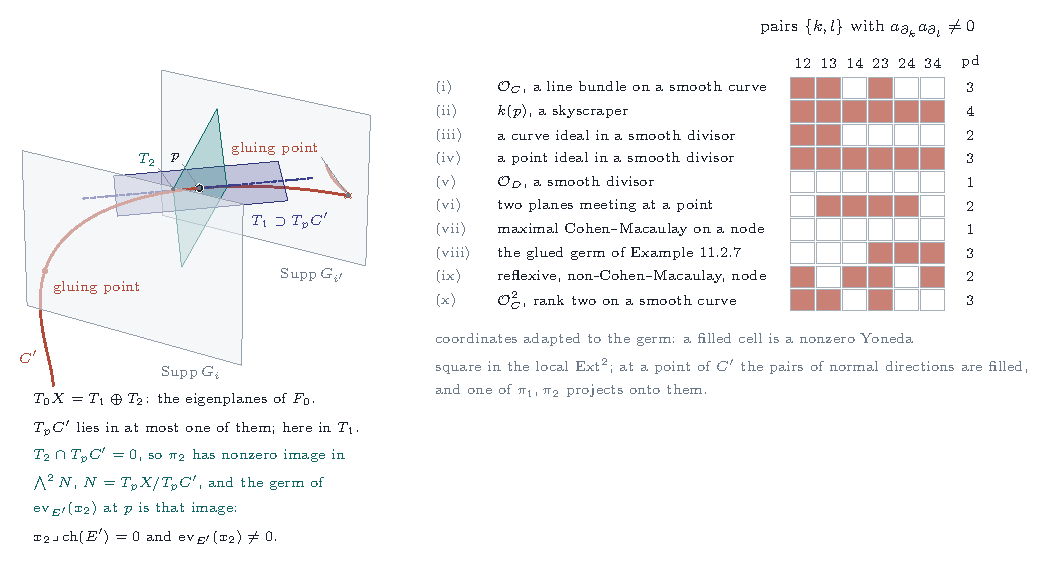
\includegraphics[width=\textwidth]{fig_quarticlocal}
\caption{\Cref{thm:quarticlocal} and \Cref{cor:markmanquarticfails}. Left: the
support of Markman's sheaf $E'$ near a point $p$ of the glued curve $C'$,
between two of the translated supports that the curve crosses at its gluing
points. The tangent space at $p$ is the sum of the eigenplanes $T_{1}$ and
$T_{2}$ of the real multiplication; the tangent line of $C'$ lies in at most
one of them, here in $T_{1}$, so $\pi_{2}$ has nonzero image in
$\bigwedge^{2}N$, $N=T_{p}X/T_{p}C'$, which is the germ of
$\operatorname{ev}_{E'}(x_{2})$ at $p$. Right: for ten germs at the origin
of $\CC^{4}$, the pairs $\{k,l\}$ of coordinate directions whose jet classes
have nonzero product in the local $\Ext^{2}$, and the projective dimension;
rows (i), (ii) and (x) are \Cref{lem:freegerm}, row (iii) is
\Cref{lem:divisorgerm}, row (vi) is \Cref{lem:localproducts}.}
\label{fig:quarticlocal}
\end{figure}

\subsection{Sextic CM fields}\label{ssec:sextic}

The dimension count of \Cref{thm:quarticobstruction} does not extend to CM
fields of degree six, for a reason of parity (\Cref{rem:sexticparity}). Let
$F=F_{0}(\sqrt{-q})$ be a sextic CM field with totally
real cubic subfield $F_{0}$, real places $\tau_{1},\tau_{2},\tau_{3}$ and $q\in
F_{0}$ totally positive, and let $X$ be a principally polarised abelian sixfold
with real multiplication by $\cO_{F_{0}}$, so that
$H^{1}(X,\CC)=U_{1}\oplus U_{2}\oplus U_{3}$ with $U_{j}$ the eigenspace of
$\tau_{j}$, of dimension four and Hodge type $(2,2)$. Let
$\theta_{j}\in H^{1,1}(X)$ be the component of the polarisation on $U_{j}$, so
that $\theta=\sum_{j}\theta_{j}$, $\theta_{j}^{3}=0$ and
$\int_{X}\theta_{1}^{2}\theta_{2}^{2}\theta_{3}^{2}=8$. For $t\in F_{0}$ and
$\varepsilon\in\{\pm1\}^{3}$ put $s_{j}=\sqrt{-1}\,\sqrt{\tau_{j}(q)}$ and
$e_{\varepsilon}=\exp\bigl(\sum_{j}(\tau_{j}(t)+\varepsilon_{j}s_{j})\theta_{j}\bigr)$,
and let $S(t,q)$ be the span of the eight $e_{\varepsilon}$. As in
\Cref{prop:quarticsecant}(i) it is a rational subspace of dimension
$8=2^{[F_{0}:\QQ]}$ of the algebra generated by the $\theta_{j}$, the Galois
group permuting the $e_{\varepsilon}$ as it permutes the CM types of $F$; for
$t=0$ it is the secant space of Markman's construction for $F$ on
$X\times\widehat{X}$ \cite[\S11.1]{Mar25c}, and
$S(t,q)=e^{\sum_{j}\tau_{j}(t)\theta_{j}}S(0,q)$. A real class
$v=\sum_{\varepsilon}w_{\varepsilon}e_{\varepsilon}$ has
$w_{-\varepsilon}=\bbar{w}_{\varepsilon}$. Write $N_{w}$ for the number of
nonzero $w_{\varepsilon}$; $A_{jj'}$ for the number of sign pairs
$(\sigma,\sigma')$ such that $w_{\varepsilon}\ne0$ for some $\varepsilon$ with
$\varepsilon_{j}=\sigma$ and $\varepsilon_{j'}=\sigma'$; $\rho_{j}$ for the rank
of the $2\times4$ matrix $(w_{\varepsilon})$ whose rows are indexed by
$\varepsilon_{j}$ and whose columns by the two other signs; and, for
$\{j,j',j''\}=\{1,2,3\}$ and $\sigma'=\pm1$, $M^{(j;j')}_{\sigma'}$ for the
$2\times2$ matrix $(w_{\varepsilon})_{\varepsilon_{j},\varepsilon_{j''}}$ with
$\varepsilon_{j'}=\sigma'$ fixed. Let $r^{k}(v)$ be the rank of the contraction
$HT^{k}(X)\to H^{*}(X,\CC)$, $\xi\mapsto\xi\lrcorner\,v$.

\begin{proposition}[The count in degree six]\label{prop:sexticcount}
Let $v\in S(t,q)$ be a nonzero real class.
\begin{enumerate}[label=\textup{(\roman*)},leftmargin=2.6em,itemsep=2pt]
\item $r^{1}(v)=12$,
  \[
    r^{2}(v)=4\,(A_{12}+A_{13}+A_{23})+\rho_{1}+\rho_{2}+\rho_{3},
    \qquad
    r^{3}(v)=8N_{w}+2\sum_{j\ne j'}\bigl(\rk M^{(j;j')}_{+}+\rk M^{(j;j')}_{-}\bigr).
  \]
  So $r^{2}(v)\le54$ and $r^{3}(v)\le112$, with equality when every
  $w_{\varepsilon}$ is nonzero and every $M^{(j;j')}_{\sigma'}$ is invertible,
  which holds outside a proper Zariski closed subset of $S(t,q)$. When $F$
  contains an imaginary quadratic field $K$ and $v$ lies in the secant plane
  of $K$, so that $N_{w}=2$, one has $(r^{2},r^{3})=(30,40)$.
\item $\chi(v,v)=\int_{X}v^{\vee}v=-64\,\Nm_{F_{0}/\QQ}(q)\sum_{\varepsilon}
  |w_{\varepsilon}|^{2}<0$. For a CM field of degree $2m$, with $X$ of dimension
  $2m$ and $2^{m}$ exponentials, the same computation gives
  $(-4)^{m}\Nm(q)\sum_{\varepsilon}|w_{\varepsilon}|^{2}$: the Euler form on
  the secant space is definite, of sign $(-1)^{m}$.
\item Let $F_{1},F_{2}$ be perfect complexes on $X$ with
  $\Ext^{<0}(F_{i},F_{i})=0$ and characters $v_{i}$ in spaces
  $S(t_{i},q_{i})$, let $A=X\times\widehat{X}$ carry the action of $F$ of
  \cite[\S11.1]{Mar25c}, transported by the exponential of a rational
  $F_{0}$-$B$-field, and put
  $E=\Phi(F_{1}\boxtimes F_{2}^{\vee})$ and $\kappa=\ch(E)e^{\ell/2}$. Then
  $r(\kappa)=r(\ch E)=r^{2}(v_{1})+144+r^{2}(v_{2})\le252$, while every class
  that stays of Hodge type over $\cD_{F}$ has rank at most
  $\dim HT^{2}(A)-\dim\cD_{F}=276-12=264$. Moreover
  $\dim\Ext^{2}(E,E)\ge r(\kappa)$, with equality if and only if each $F_{i}$
  has
  \[
    \dim\Ext^{k}(F_{i},F_{i})=1,\ 12,\ r^{2}(v_{i}),\ e_{3},\ r^{2}(v_{i}),\ 12,\ 1
    \quad(k=0,\dots,6),
  \]
  where $e_{3}=2r^{2}(v_{i})-22-\chi(v_{i},v_{i})$,
  and this profile is compatible with the bound $e_{3}\ge r^{3}(v_{i})$ exactly
  when $\chi(F_{i},F_{i})\le-(r^{3}(v_{i})-2r^{2}(v_{i})+22)$, that is
  $\chi(F_{i},F_{i})\le-26$ for $v_{i}$ general in its secant space, and
  $\chi(F_{i},F_{i})\le-2$ when $N_{w}=2$.
\item If $t_{1}=t_{2}=0$ and $q_{1}=q_{2}=q$, then $\kappa$ is invariant
  under $G_{F}$, and so is a Hodge class on every member of the
  $(F,2,1)$-family.
\end{enumerate}
\end{proposition}

\begin{proof}
(i) Choose a basis $x_{j1},x_{j2}$ of $U_{j}^{1,0}$ and $y_{j1},y_{j2}$ of
$U_{j}^{0,1}$ with $\theta_{j}=x_{j1}y_{j1}+x_{j2}y_{j2}$, and let
$\omega_{j}=y_{j1}y_{j2}$ span $\bigwedge^{2}U_{j}^{0,1}$. Then
$H^{*}(X,\CC)$ and $HT^{*}(X)=\bigwedge^{*}(H^{0,1}\oplus T)$ are the tensor
products over $j$ of the corresponding algebras of the three factors,
$HT^{k}(X)=\bigoplus_{a_{1}+a_{2}+a_{3}=k}HT^{a_{1}}_{1}\otimes HT^{a_{2}}_{2}
\otimes HT^{a_{3}}_{3}$, and contraction is compatible with the factorisation;
$v=\sum_{\varepsilon}w_{\varepsilon}\bigotimes_{j}e^{\lambda_{j}(\varepsilon_{j})\theta_{j}}$
with $\lambda_{j}(\pm1)=\tau_{j}(t)\pm s_{j}$, two distinct numbers. The blocks
of $HT^{k}(X)$ shift the three Hodge bidegrees of $H^{*}(X)$ by different
amounts, so their images are independent and $r^{k}(v)$ is the sum of their
ranks. Inside a block the bookkeeping rests on two facts about one factor:
the two classes $e^{\lambda_{j}(\pm1)\theta_{j}}$ are linearly independent,
and so are the subspaces $U_{j}^{0,1}e^{\lambda_{j}(\pm1)\theta_{j}}$ of
$H^{*}(U_{j})$, since $u\,e^{\lambda\theta_{j}}=u+\lambda\,u\theta_{j}$ for
$u\in U_{j}^{0,1}$; whereas $\omega_{j}e^{\lambda\theta_{j}}=\omega_{j}$ for
every $\lambda$, so that the summands of a block through $HT^{2}_{j}$ share the
factor $\omega_{j}$ and are combined, not juxtaposed. On one factor,
contraction into $e^{\lambda\theta_{j}}$ is as follows. For $\xi\in HT^{1}_{j}$,
$\xi\lrcorner\,e^{\lambda\theta_{j}}=y^{\lambda}(\xi)\,e^{\lambda\theta_{j}}$ with
$y^{\lambda}(\xi)=\xi^{0,1}+\lambda\,\xi_{T}\lrcorner\,\theta_{j}\in
U_{j}^{0,1}$, as in \Cref{lem:bfield}(i); $y^{\lambda}$ is onto, its kernel
$K^{\lambda}_{j}$ has dimension two, and
$HT^{1}_{j}=K^{\lambda_{j}(+1)}_{j}\oplus K^{\lambda_{j}(-1)}_{j}$ because
$\lambda_{j}(+1)\ne\lambda_{j}(-1)$ and $\xi_{T}\lrcorner\,\theta_{j}$
determines $\xi_{T}$. For $\xi\in HT^{2}_{j}$, since $\omega_{j}\theta_{j}=0$,
one finds $\omega_{j}\lrcorner\,e^{\lambda\theta_{j}}=\omega_{j}$,
$(y_{ja}\otimes\partial_{x_{jb}})\lrcorner\,e^{\lambda\theta_{j}}=\pm\lambda\,
\omega_{j}$ for $a\ne b$ and $0$ for $a=b$, and
$(\partial_{x_{j1}}\wedge\partial_{x_{j2}})\lrcorner\,e^{\lambda\theta_{j}}
=\pm\lambda^{2}\omega_{j}$: the image of $HT^{2}_{j}$ is the line
$\CC\omega_{j}$, $\xi\lrcorner\,e^{\lambda\theta_{j}}=c(\xi,\lambda)\,\omega_{j}$,
and the pairs $\bigl(c(\xi,\lambda_{j}(+1)),c(\xi,\lambda_{j}(-1))\bigr)$ fill
$\CC^{2}$. For $k\ge3$, $HT^{k}_{j}$ kills $e^{\lambda\theta_{j}}$, because
every element of it contains $\omega_{j}$ or $\partial_{x_{j1}}\wedge
\partial_{x_{j2}}$ together with a further factor, and the further factor
kills $\omega_{j}$.

Now count. The block $HT^{1}_{j}$ acts on $v$ by
$\xi\mapsto\sum_{\varepsilon}w_{\varepsilon}\,y^{\lambda_{j}(\varepsilon_{j})}(\xi)
\bigotimes_{j'}e^{\lambda_{j'}(\varepsilon_{j'})\theta_{j'}}$; on the summand
$K^{\lambda_{j}(-\sigma)}_{j}$ only the $\varepsilon$ with
$\varepsilon_{j}=\sigma$ contribute, and they map it isomorphically onto
$U_{j}^{0,1}$ tensored with a nonzero class as soon as one such
$w_{\varepsilon}$ is nonzero. Both signs occur in the support of a nonzero real
$w$, since $w_{-\varepsilon}=\bbar{w}_{\varepsilon}$, so the block has rank $4$
and $r^{1}(v)=12$. The block $HT^{1}_{j}\otimes HT^{1}_{j'}$ is the sum of the
four summands $K^{\lambda_{j}(-\sigma)}_{j}\otimes K^{\lambda_{j'}(-\sigma')}_{j'}$,
each of dimension four; the summand indexed by $(\sigma,\sigma')$ maps
isomorphically onto $U_{j}^{0,1}\otimes U_{j'}^{0,1}$ tensored with the class
$\sum_{\sigma''}w_{\varepsilon}e^{\lambda_{j''}(\sigma'')\theta_{j''}}$, which
is nonzero exactly when the pair $(\sigma,\sigma')$ occurs in the support, and
to zero otherwise; so the block has rank $4A_{jj'}$. The block $HT^{2}_{j}$
maps $\xi$ to $\sum_{\sigma}c(\xi,\lambda_{j}(\sigma))\,z_{\sigma}$ with
$z_{\sigma}=\omega_{j}\otimes\sum_{\mu}w_{\sigma\mu}e_{\mu}$, where $\mu$ runs
over the four sign patterns of the other two places and the $e_{\mu}$ are
independent; as $(c(\xi,\lambda_{j}(+1)),c(\xi,\lambda_{j}(-1)))$ fills
$\CC^{2}$, the rank is the dimension of the span of $z_{+},z_{-}$, which is
$\rho_{j}$. This gives $r^{2}(v)$. In degree three the block
$HT^{1}_{1}\otimes HT^{1}_{2}\otimes HT^{1}_{3}$ is the sum of eight summands
$\bigotimes_{j}K^{\lambda_{j}(-\varepsilon_{j})}_{j}$, of dimension eight, on
each of which exactly one term of $v$ acts, isomorphically when
$w_{\varepsilon}\ne0$ and by zero otherwise: rank $8N_{w}$. The block
$HT^{2}_{j}\otimes HT^{1}_{j'}$ factors through $\CC^{2}\otimes HT^{1}_{j'}$
by $c\otimes\mathrm{id}$, which is onto, and on
$\CC^{2}\otimes K^{\lambda_{j'}(-\sigma')}_{j'}$ the map is
$M^{(j;j')}_{\sigma'}\otimes y^{\lambda_{j'}(\sigma')}$ followed by tensoring
with independent classes, of rank $2\rk M^{(j;j')}_{\sigma'}$; the two values
of $\sigma'$ give independent images. The blocks $HT^{3}_{j}$ contribute
nothing. This gives $r^{3}(v)$. The maximal values are $48+6=54$ and
$64+6\cdot8=112$; the conditions for them are the nonvanishing of the
$w_{\varepsilon}$ and of the determinants of the $M^{(j;j')}_{\sigma'}$, which
are polynomials in the coordinates of $v$, nonzero on $S(t,q)$. If $F\supseteq K$
and $v$ lies in the secant plane of $K$, the support of $w$ is a pair
$\{\varepsilon_{0},-\varepsilon_{0}\}$, the two CM types of $F$ induced from
$K$; then $A_{jj'}=2$, $\rho_{j}=2$, $N_{w}=2$ and every
$M^{(j;j')}_{\sigma'}$ has one nonzero entry, so $(r^{2},r^{3})=(24+6,16+24)$.

(ii) Since $\theta_{j}^{3}=0$, $\theta^{2m}=\frac{(2m)!}{2^{m}}\theta_{1}^{2}
\cdots\theta_{m}^{2}$, and $\int_{X}\theta^{2m}/(2m)!=1$ gives
$\int_{X}\theta_{1}^{2}\cdots\theta_{m}^{2}=2^{m}$ and
$\int_{X}\exp(\sum_{j}c_{j}\theta_{j})=\prod_{j}c_{j}^{2}$. The dual of
$e^{\lambda\theta_{j}}$ is $e^{-\lambda\theta_{j}}$, so
$\int_{X}e_{\varepsilon}^{\vee}e_{\varepsilon'}=\prod_{j}\bigl(\lambda_{j}(\varepsilon'_{j})
-\lambda_{j}(\varepsilon_{j})\bigr)^{2}$, which is $0$ unless
$\varepsilon'=-\varepsilon$, where it is $\prod_{j}(2s_{j})^{2}=(-4)^{m}\Nm(q)$.
Hence $\chi(v,v)=(-4)^{m}\Nm(q)\sum_{\varepsilon}w_{\varepsilon}w_{-\varepsilon}
=(-4)^{m}\Nm(q)\sum_{\varepsilon}|w_{\varepsilon}|^{2}$.

(iii) As in the proof of \Cref{thm:quarticobstruction}(i), $r(\kappa)=r(\ch E)$
by \Cref{lem:bfield}(i), and $\Phi$ identifies $r(\ch E)$ with the rank of
contraction from $HT^{2}(X\times X)=\bigoplus_{a+b=2}HT^{a}(X)\otimes HT^{b}(X)$
into $v_{1}\boxtimes v_{2}$; the block $HT^{1}\otimes HT^{1}$ contributes
$r^{1}(v_{1})r^{1}(v_{2})=144$ and the other two contribute
$r^{2}(v_{1})+r^{2}(v_{2})$, by the type argument given there. The tangent
space $T_{[A]}\cD_{F}\subseteq H^{1}(T_{A})$, of dimension $mn^{2}=12$, kills
every class that stays of Hodge type along $\cD_{F}$, as in
\Cref{prop:p2primelocus}(i), and $\dim HT^{2}(A)=66+144+66$. By the K\"unneth
formula, with $\Ext^{<0}=0$,
$\dim\Ext^{2}(E,E)=e_{0}e_{2}'+e_{1}e_{1}'+e_{2}e_{0}'$ where
$e_{k}=\dim\Ext^{k}(F_{1},F_{1})$ and $e_{k}'=\dim\Ext^{k}(F_{2},F_{2})$; the
commutative square $\sigma\circ\operatorname{ev}=(\,\cdot\,)\lrcorner\ch$ of
\Cref{setup:criterion}, valid in every degree, gives $e_{k}\ge r^{k}(v_{1})$
and $e_{k}'\ge r^{k}(v_{2})$, and $e_{0},e_{0}'\ge1$. So
$\dim\Ext^{2}(E,E)\ge r^{2}(v_{2})+144+r^{2}(v_{1})$, with equality if and
only if $e_{0}=e_{0}'=1$, $e_{1}=e_{1}'=12$, $e_{2}=r^{2}(v_{1})$ and
$e_{2}'=r^{2}(v_{2})$. Serre duality on the sixfold gives $e_{k}=e_{6-k}$, so
$\chi(F_{i},F_{i})=2(e_{0}-e_{1}+e_{2})-e_{3}=2r^{2}(v_{i})-22-e_{3}$, and by
Riemann--Roch on an abelian variety $\chi(F_{i},F_{i})=\chi(v_{i},v_{i})$,
which is (ii); this determines $e_{3}$, and $e_{3}\ge r^{3}(v_{i})$ is the
stated inequality. With the maximal ranks it reads
$\chi\le-(112-108+22)=-26$, and with $N_{w}=2$ it reads
$\chi\le-(40-60+22)=-2$.

(iv) The proof of \Cref{thm:quarticobstruction}(iii) applies with three
factors in place of two: for $t=0$ the classes $e_{\varepsilon}\boxtimes
e_{\varepsilon'}^{\vee}$, the correspondence $Z\mapsto\ch(\Phi(Z))e^{\ell/2}$
and the Poincar\'e class decompose as tensor products over $j$ of classes of
even degree, on each factor $\sqrt{-q}$ acts as in the imaginary quadratic
construction with $d$ replaced by $\tau_{j}(q)$, and the identities of
\Cref{prop:flatall} at $n=2$ show that each image is a multiple of an
exponential of $\eta_{j}$ or of a Weil class of the $j$-th factor, invariant
under the special unitary group of that factor; $G_{F}(\RR)$ is the product of
the three, and is Zariski dense in $G_{F}$. Statement (iv) is the case
$[F:\QQ]=6$ of \cite[Proposition~10.2.1(1)]{Mar25c}, with the inclusion
$\widetilde\phi(B\otimes B)\subset A$ of \cite[p.~33]{Mar25c}, which Markman
proves for every CM field in his conventions for $\Phi$ and for the twist; we
make no claim of priority.
\end{proof}

\begin{remark}[The special role of degree four]
\label{rem:sexticparity}
In \Cref{thm:quarticobstruction} the equality $\dim\Ext^{2}(E,E)=r(\kappa)$
determines the whole Ext profile of each factor, because on a fourfold
$\Ext^{2}$ is the middle degree and Serre duality supplies the rest; the Euler
characteristic of a minimal factor is then the small positive integer
$r^{2}-14$, the Euler form on the secant space being positive definite, and
the arithmetic of \Cref{prop:quarticother} excludes it. On a sixfold the same
equality fixes $\Ext^{0}$, $\Ext^{1}$ and $\Ext^{2}$ and leaves the middle
group $\Ext^{3}$ free, and the Euler form has the opposite sign:
$\chi(F_{i},F_{i})=-64\Nm(q)\sum|w_{\varepsilon}|^{2}$ is a negative integer
that $e_{3}$ absorbs. So no dimension count excludes a minimal Orlov product
over a sextic field, and none does over any CM field of degree $2m\ge6$,
where $\Ext^{3},\dots,\Ext^{m}$ are free and the Euler form has sign
$(-1)^{m}$. What \Cref{prop:sexticcount}(iii) leaves for such an object is the
profile displayed there, with $\chi(F_{i},F_{i})\le-26$ for a general secant
character, and the flat twisted character of (iv), which stays of Hodge type
over the whole twelve-dimensional period domain. Whether a sheaf with that
profile exists on a sixfold with real multiplication by a cubic field is not
known; nothing in \Cref{thm:quarticobstruction} bears on it. A certificate
of the kind of \Cref{thm:twistedcert} for a sextic field would be an Orlov
product of such sheaves, with $\dim\Ext^{2}(E,E)=r(\kappa)\le252$ on the
twelvefold, whose twisted character has a nonzero component in the Weil
classes $W_{F}(A)$; flatness does not give that component, and
\Cref{lem:sexticweil} computes it. In degree six as in degree four, the Orlov
products never reach the rank of a class of general shape: $r(\kappa)\le252$
against $264$, and $r(\kappa)\le104$ against $112$.
\end{remark}

The count of \Cref{prop:sexticcount}(iii) is a condition on the Euler
characteristic of the character alone, so it can be tested on the lattice of
integral characters, as \Cref{prop:quarticother} tests the quartic one. In
degree four the test excludes every minimal character. In degree six it can
exclude an integral character only if $-26<\chi(v,v)<0$
(\Cref{prop:sexticintegral}(i),(ii)), and it excludes neither of the integral
classes $\operatorname{Re}e^{\sqrt{-1}\,\theta}$ and
$\operatorname{Im}e^{\sqrt{-1}\,\theta}$ (\Cref{prop:sexticintegral}(iv)). For
$t=0$, the case in which
\Cref{prop:sexticcount}(iv) makes $\kappa$ flat, put
$B_{j}=1-\tfrac12\tau_{j}(q)\,\theta_{j}^{2}$, so that
$e^{\pm s_{j}\theta_{j}}=B_{j}\pm s_{j}\theta_{j}$, and for
$c_{0},c_{3}\in\QQ$ and $f,g\in F_{0}$ let
\[
  v(c_{0},f,g,c_{3})=c_{0}B_{1}B_{2}B_{3}
  +\sum_{j}\tau_{j}(f)\,\theta_{j}B_{k}B_{l}
  +\sum_{j}\tau_{j}(g)\,B_{j}\theta_{k}\theta_{l}
  +c_{3}\,\theta_{1}\theta_{2}\theta_{3},
\]
where $\{j,k,l\}=\{1,2,3\}$ in each sum.

\begin{proposition}[Integral flat characters in degree six]
\label{prop:sexticintegral}
Keep the notation of \Cref{prop:sexticcount}.
\begin{enumerate}[label=\textup{(\roman*)},leftmargin=2.6em,itemsep=2pt]
\item For every perfect complex $F$ on a complex torus of dimension six,
  $\chi(F,F)$ is even. So the condition of \Cref{prop:sexticcount}(iii)
  holds for every $F$ whose character has $N_{w}=2$.
\item For every nonzero real $v\in S(t,q)$, $r^{3}(v)-2r^{2}(v)\le4$, with
  equality only if $(r^{2}(v),r^{3}(v))=(54,112)$. So for every shape the
  condition of \Cref{prop:sexticcount}(iii) is implied by
  $\chi(F_{i},F_{i})\le-26$.
\item The rational points of $S(0,q)$ are the classes $v(c_{0},f,g,c_{3})$,
  and
  \[
    \chi(v,v)=-8\bigl(\Nm(q)\,c_{0}^{2}+\Tr\bigl(\Nm(q)\,q^{-1}f^{2}\bigr)
    +\Tr(q\,g^{2})+c_{3}^{2}\bigr).
  \]
\item For $q=1$, the classes $\operatorname{Re}e^{\sqrt{-1}\,\theta}=v(1,0,-1,0)$
  and $\operatorname{Im}e^{\sqrt{-1}\,\theta}=v(0,1,0,-1)$ are integral
  points of $S(0,1)$ with $\chi=-32$ and $N_{w}=2$, so they satisfy the
  condition of \Cref{prop:sexticcount}(iii).
\end{enumerate}
\end{proposition}

\begin{proof}
(i) The Chern character $v=\ch(F)$ is integral, as in the proof of
\Cref{thm:quarticobstruction}(ii), and $\chi(F,F)=\int_{X}v^{\vee}v$ by
Riemann--Roch. Write $v=\sum_{k}v_{2k}$, so that
$\int_{X}v^{\vee}v=\sum_{k}(-1)^{k}\int_{X}v_{2k}v_{12-2k}$. The terms $k$ and
$6-k$ are equal, since $(-1)^{k}=(-1)^{6-k}$ and classes of even degree
commute, so they contribute an even number when $k\ne3$. For $k=3$ write
$v_{6}=\sum_{I}a_{I}e_{I}$ in the basis of $\bigwedge^{6}H^{1}(X,\ZZ)$ given
by the products $e_{I}$ of six elements of a basis of $H^{1}(X,\ZZ)$; since
$e_{I}e_{I}=0$ and $e_{I}e_{J}=e_{J}e_{I}$, $v_{6}^{2}=2\sum_{I<J}a_{I}a_{J}
e_{I}e_{J}$ is even. For $N_{w}=2$ the condition of
\Cref{prop:sexticcount}(iii) is $\chi(F,F)\le-2$, and $\chi(F,F)$ is a
negative even integer by \Cref{prop:sexticcount}(ii).

(ii) For $j$ and $\sigma=\pm1$ let $W_{j,\sigma}$ be the $2\times2$ slice
$(w_{\varepsilon})_{\varepsilon_{j}=\sigma}$, with rows and columns indexed by
the signs at the two other places. The matrices $M^{(j';j)}_{\sigma}$ are
$W_{j,\sigma}$ and its transpose, so
$\sum_{j\ne j'}\bigl(\rk M^{(j;j')}_{+}+\rk M^{(j;j')}_{-}\bigr)
=2\sum_{j,\sigma}\rk W_{j,\sigma}$. Since $w_{-\varepsilon}=\bbar{w}_{\varepsilon}$,
$W_{j,-}$ is the complex conjugate of $W_{j,+}$ with its rows and its columns
reversed, so the two slices have the same rank $k_{j}$. Let $S$ be the support
of $w$ and $N=N_{w}=|S|$. By \Cref{prop:sexticcount}(i),
\begin{equation}\label{eq:sexticexcess}
  r^{3}(v)-2r^{2}(v)=8N-8\,(A_{12}+A_{13}+A_{23})
  +\sum_{j}\bigl(8k_{j}-2\rho_{j}\bigr).
\end{equation}
The set $S$ is stable under $\varepsilon\mapsto-\varepsilon$, which exchanges
the two slices along each place; so $N$ is even, each slice has $N/2$ nonzero
entries, $k_{j}\ge1$, and $A_{jj'}\in\{2,4\}$, the projection of $S$ to the
signs at $j$ and $j'$ being stable under negation. Also $1\le\rho_{j}\le2$ and
$k_{j}\le2$, and a slice whose nonzero entries lie in one row or one column
has rank one. If $\rho_{j}=1$, then $w_{\varepsilon}=a_{\varepsilon_{j}}
W(\varepsilon')$, with $\varepsilon'$ the signs at the two other places, so
every slice along a place $j'\ne j$ is $a\otimes(\text{a row of }W)$ and
$k_{j'}\le1$. Now take the four values of $N$ in turn.

If $N=8$, every $A_{jj'}$ is $4$ and \eqref{eq:sexticexcess} is
$-32+\sum_{j}(8k_{j}-2\rho_{j})$. When every $\rho_{j}$ is $2$ this is at most
$-32+3\cdot12=4$, with equality exactly when every $k_{j}$ is $2$, and then
$r^{2}=48+6=54$ and $r^{3}=64+48=112$. When some $\rho_{j}$ is $1$, the two
other $k$ are at most $1$ and \eqref{eq:sexticexcess} is at most
$-32+14+6+6=-6$.

If $N=6$, $S$ misses one pair $\{\pm\varepsilon_{0}\}$. As $\varepsilon_{0}$
and $-\varepsilon_{0}$ differ at every place, they never have the same signs
at two places, so every sign pair at two places occurs in $S$, every
$A_{jj'}$ is $4$, and \eqref{eq:sexticexcess} is at most $48-96+3\cdot14=-6$.

If $N=4$, $S=\{\pm\varepsilon,\pm\varepsilon'\}$, and after replacing
$\varepsilon'$ by $-\varepsilon'$ if necessary, $\varepsilon$ and
$\varepsilon'$ differ at exactly one place $j$. For the two other places $k$
and $l$ one has $A_{kl}=2$ and $A_{jk}=A_{jl}=4$. The two nonzero entries of
a slice along $k$ are $w_{\pm\varepsilon}$ and $w_{\pm\varepsilon'}$ with the
same sign, whose indices agree at $l$; they lie in one row or one column, so
$k_{k}=1$, and likewise $k_{l}=1$. Hence \eqref{eq:sexticexcess} is at most
$32-80+8\,(2+1+1)-6=-22$.

If $N=2$, $S=\{\pm\varepsilon_{0}\}$, every $A_{jj'}$ is $2$, every $k_{j}$ is
$1$, and every $\rho_{j}$ is $2$, the two slices along $j$ having their
nonzero entries at different positions; so \eqref{eq:sexticexcess} is
$16-48+24-12=-20$, the value $40-60$ of \Cref{prop:sexticcount}(i).

So $r^{3}-2r^{2}\le4$, with equality only at $(54,112)$, and the threshold
$r^{3}-2r^{2}+22$ of \Cref{prop:sexticcount}(iii) is at most $26$.

(iii) Since $\theta_{j}^{3}=0$ and $s_{j}^{2}=-\tau_{j}(q)$,
$e^{\pm s_{j}\theta_{j}}=B_{j}\pm s_{j}\theta_{j}$, so the eight exponentials
and the eight products $\prod_{j}\beta_{j}$ with $\beta_{j}\in\{B_{j},\theta_{j}\}$
span the same complex space, the change of basis being the tensor cube of an
invertible $2\times2$ matrix. The Galois group permutes the $\tau_{j}$, the
$\theta_{j}$ and the $B_{j}$ compatibly, so $\sum_{a}C_{a}\prod_{j}\beta_{j}$,
indexed by the subsets $a$ of $\{1,2,3\}$ with $\beta_{j}=\theta_{j}$ for
$j\in a$, is rational exactly when $C_{\pi(a)}=\sigma(C_{a})$ for every
$\sigma$ inducing $\pi$; the stabiliser of $\{j\}$, and of its complement,
is the stabiliser of $\tau_{j}$, which gives the form $v(c_{0},f,g,c_{3})$.
The involution $v\mapsto v^{\vee}$ and the integral are multiplicative over
the three factors, with $\int_{X}\theta_{1}^{2}\theta_{2}^{2}\theta_{3}^{2}=8$;
on one factor $B_{j}^{\vee}B_{j}=1-\tau_{j}(q)\theta_{j}^{2}$,
$\theta_{j}^{\vee}\theta_{j}=-\theta_{j}^{2}$ and the mixed products are odd
in $\theta_{j}$. So
$\chi(v,v)=-8\sum_{a}C_{a}^{2}\prod_{j\notin a}\tau_{j}(q)$, which is the
formula.

(iv) For $q=1$, $s_{j}=\sqrt{-1}$ and $e_{(1,1,1)}=\prod_{j}e^{\sqrt{-1}\,
\theta_{j}}=e^{\sqrt{-1}\,\theta}$. The polarisation is principal, so each
$\theta^{k}/k!$ is integral, and so are the real and imaginary parts
$\sum_{k}(-1)^{k}\theta^{2k}/(2k)!$ and $\sum_{k}(-1)^{k}\theta^{2k+1}/(2k+1)!$.
They are $\tfrac12(e_{(1,1,1)}+e_{(-1,-1,-1)})$ and
$\tfrac1{2\sqrt{-1}}(e_{(1,1,1)}-e_{(-1,-1,-1)})$, so $N_{w}=2$ and
$\chi=-64\,(\tfrac14+\tfrac14)=-32$ by \Cref{prop:sexticcount}(ii); expanding
$\prod_{j}(B_{j}+\sqrt{-1}\,\theta_{j})$ gives the coordinates.
\end{proof}

The flatness of \Cref{prop:sexticcount}(iv) makes $\kappa$ a Hodge class on
every member of the family, but in degree four the Hodge classes of a very
general member are the products of divisor classes and the Weil classes
$W_{F}(A)$ (\cite[Proposition~17.3(iii)]{paperI}), and only a nonzero component of
$\kappa$ in $W_{F}(A)$ bears on $\mathbf{W}(F,2,1)$. We compute that
component. Keep the notation of \Cref{prop:sexticcount}, with $t_{1}=t_{2}=0$,
$q_{1}=q_{2}=q$ and trivial $B$-field, put $d_{j}=\tau_{j}(q)$, and let
$\Psi(Z)=\ch(\Phi(Z))e^{\ell/2}$ as in \Cref{prop:flatall}, so that
$\kappa(v_{1},v_{2})=\Psi(v_{1}\boxtimes v_{2}^{\vee})$ for the characters
$v_{i}$ of $F_{i}$. As in the proof of \Cref{prop:sexticcount}(iv),
$H^{1}(A,\CC)$ is the sum of three factors $U_{j}\oplus U_{j}^{\vee}$, on each
of which $\sqrt{-q}$ acts as in the imaginary quadratic construction with
$\beta=\theta_{j}$ and $d=d_{j}$. On the $j$-th factor write
$\widehat\theta_{j}$ and $\ell_{j}$ for the components of the dual
polarisation and of the Poincar\'e class, and put
$\gamma_{j}=d_{j}\theta_{j}-\widehat\theta_{j}$, as in \cite[(33)]{paperI},
and $\eta_{j}=d_{j}\theta_{j}+\widehat\theta_{j}$, a positive multiple of the
polarisation of the factor for which $\sqrt{-q}$ is anti-self-adjoint
(\cite[Proposition~15.19(i)]{paperI}). For $\sigma=\pm1$ let $\tau_{j,\sigma}$ be the
embedding of $F$ over $\tau_{j}$ with
$\tau_{j,\sigma}(\sqrt{-q})=\sigma\sqrt{-1}\,\sqrt{\tau_{j}(q)}=\sigma s_{j}$,
and $V_{j,\sigma}\subset H^{1}(A,\CC)$ its eigenspace, of dimension four. By
\cite[Theorem~15.2(ii)]{paperI} with $n=2$ and $d=d_{j}$, the line
$\bigwedge^{4}V_{j,\sigma}$ is spanned by
\begin{equation}\label{eq:sexticomega}
  \omega_{j,\sigma}=-\frac{1}{2d_{j}^{2}}\bigl(\gamma_{j}-\sigma s_{j}\ell_{j}\bigr)^{2},
\end{equation}
so the six classes $\omega_{j,\sigma}$ span $W_{F}(A)\otimes\CC$. Since
$\eta_{j}$ pairs $V_{j,+}$ with $V_{j,-}$, the products $\eta_{i}\eta_{k}$ lie
in summands of $H^{4}(A,\CC)=\bigwedge^{4}\bigl(\bigoplus_{j,\sigma}
V_{j,\sigma}\bigr)$ other than the six lines $\bigwedge^{4}V_{j,\sigma}$. Let
$\kappa_{j,\sigma}(v_{1},v_{2})$ be the coefficient of $\omega_{j,\sigma}$ in
the component of $\kappa(v_{1},v_{2})$ in $\bigwedge^{4}V_{j,\sigma}$; the
\emph{$F$-Weil part} of $\kappa$ is
$\sum_{j,\sigma}\kappa_{j,\sigma}\,\omega_{j,\sigma}$, its component in
$W_{F}(A)\otimes\CC$. For $\varepsilon\in\{\pm1\}^{3}$ let
$\varepsilon^{(j)}$ be the sign vector that agrees with $\varepsilon$ at $j$
and only there.

\begin{lemma}[The $F$-Weil part of an Orlov product]\label{lem:sexticweil}
Let $v_{i}=\sum_{\varepsilon}w^{i}_{\varepsilon}e_{\varepsilon}\in S(0,q)$ for
$i=1,2$.
\begin{enumerate}[label=\textup{(\roman*)},leftmargin=2.6em,itemsep=2pt]
\item The degree-four part of $\kappa(v_{1},v_{2})$ is a quadratic form in the
  $\eta_{j}$ plus $\sum_{j,\sigma}\kappa_{j,\sigma}\,\omega_{j,\sigma}$, with
  \[
    \kappa_{j,\sigma}(v_{1},v_{2})=-16\Nm(q)\,\tau_{j}(q)
    \sum_{\varepsilon_{j}=\sigma}w^{1}_{\varepsilon}\,w^{2}_{\varepsilon^{(j)}}.
  \]
\item Let $v=v(c_{0},f,g,c_{3})$ be rational, and for $\{j,k,l\}=\{1,2,3\}$
  write $f_{j}=\tau_{j}(f)$, $g_{j}=\tau_{j}(g)$ and $q_{j}=\tau_{j}(q)$. The
  numbers
  \begin{align*}
    R_{j}&=c_{0}^{2}+\frac{f_{k}^{2}}{q_{k}}+\frac{f_{l}^{2}}{q_{l}}
      +\frac{g_{j}^{2}}{q_{k}q_{l}}-\frac{1}{q_{j}}\Bigl(f_{j}^{2}
      +\frac{g_{l}^{2}}{q_{k}}+\frac{g_{k}^{2}}{q_{l}}
      +\frac{c_{3}^{2}}{q_{k}q_{l}}\Bigr),\\
    I_{j}&=c_{0}f_{j}+\frac{f_{k}g_{l}}{q_{k}}+\frac{f_{l}g_{k}}{q_{l}}
      +\frac{c_{3}g_{j}}{q_{k}q_{l}}
  \end{align*}
  are $\tau_{j}(R)$ and $\tau_{j}(I)$ for elements $R,I\in F_{0}$. Put
  $\Omega(v)=R+2I/\sqrt{-q}\in F$. Then
  \[
    \kappa_{j,\sigma}(v,v)=-\Nm(q)\,\tau_{j}(q)\,\tau_{j,\sigma}\bigl(\Omega(v)\bigr).
  \]
  So the $F$-Weil part of $\kappa(v,v)$ is zero if $R=I=0$, and otherwise
  all six $\kappa_{j,\sigma}(v,v)$ are nonzero.
\item If $v_{1}$ and $v_{2}$ are supported on one pair
  $\{\varepsilon_{0},-\varepsilon_{0}\}$, the $F$-Weil part of
  $\kappa(v_{1},v_{2})$ is zero. For $q=1$, $F$ contains
  $K=\QQ(\sqrt{-1})$, the classes $\operatorname{Re}e^{\sqrt{-1}\,\theta}$ and
  $\operatorname{Im}e^{\sqrt{-1}\,\theta}$ span the plane $P_{\theta}$ of
  \cite[Definition~14.4]{paperI} with $d=1$, and for
  $v_{i}=a_{i}\operatorname{Re}e^{\sqrt{-1}\,\theta}
  +b_{i}\operatorname{Im}e^{\sqrt{-1}\,\theta}$ with $a_{i},b_{i}\in\QQ$ the
  class $\kappa(v_{1},v_{2})$ lies in $\QQ[\eta]\oplus W_{K}(A)$, where
  $\eta=\theta+\widehat\theta$ and $W_{K}(A)\subseteq H^{12}(A,\QQ)$ are the
  Weil classes of $K$ on the twelvefold (\cite[Proposition~17.10]{paperI}); its part of
  degree at most four is
  \[
    -32(a_{1}a_{2}+b_{1}b_{2})+16(a_{1}b_{2}-a_{2}b_{1})\,\eta
    +4(a_{1}a_{2}+b_{1}b_{2})\,\eta^{2}.
  \]
\end{enumerate}
\end{lemma}

\begin{proof}
(i) The classes $e_{\varepsilon}\boxtimes e_{\varepsilon'}^{\vee}
=\bigotimes_{j}\bigl(e^{\varepsilon_{j}s_{j}\theta_{j}}\boxtimes
e^{-\varepsilon'_{j}s_{j}\theta_{j}}\bigr)$ and $\Psi$ decompose over the three
factors, as in the proof of \Cref{prop:sexticcount}(iv), and on the $j$-th
factor the two identities of \Cref{prop:flatall} at $n=2$ read, with their
constants,
\[
  \Psi_{j}\bigl(e^{\sigma s_{j}\theta_{j}}\boxtimes e^{\sigma s_{j}\theta_{j}}\bigr)
  =-4d_{j}\,e^{\sigma(s_{j}/2d_{j})\eta_{j}},
  \qquad
  \Psi_{j}\bigl(e^{\sigma s_{j}\theta_{j}}\boxtimes e^{-\sigma s_{j}\theta_{j}}\bigr)
  =\tfrac12\bigl(\gamma_{j}-\sigma s_{j}\ell_{j}\bigr)^{2}
  =-d_{j}^{2}\,\omega_{j,\sigma},
\]
since $s_{j}^{2}=-d_{j}$. So
$\Psi(e_{\varepsilon}\boxtimes e_{\varepsilon'}^{\vee})$ is the product over
$j$ of the first class where $\varepsilon'_{j}=-\varepsilon_{j}$ and of the
second where $\varepsilon'_{j}=\varepsilon_{j}$. In degree four a product with
two or three factors of the second kind vanishes, one with none is a
quadratic form in the $\eta_{j}$, and one with exactly one, at $j$, has
$\varepsilon'=\varepsilon^{(j)}$ and equals
$-d_{j}^{2}\prod_{i\ne j}(-4d_{i})\,\omega_{j,\varepsilon_{j}}
=-16\Nm(q)\,d_{j}\,\omega_{j,\varepsilon_{j}}$. Summing
$w^{1}_{\varepsilon}w^{2}_{\varepsilon'}\Psi(e_{\varepsilon}\boxtimes
e_{\varepsilon'}^{\vee})$ over $\varepsilon$ and $\varepsilon'$ gives (i).

(ii) An element $h$ of the Galois group that fixes the place $j$ permutes
the two others, so it fixes $R_{j}$ and $I_{j}$, which are symmetric in $k$
and $l$; hence $R_{j},I_{j}\in\tau_{j}(F_{0})$, and moving $j$ by the Galois
group shows that they are the conjugates of two elements of $F_{0}$. Write
$\varepsilon=(\sigma,\mu)$ with $\mu$ the signs at $k$ and $l$, so that
$\varepsilon^{(j)}=(\sigma,-\mu)$. Since $e^{\pm s_{i}\theta_{i}}=B_{i}\pm
s_{i}\theta_{i}$, the class $v=\sum_{a}C_{a}\prod_{i\in a}\theta_{i}
\prod_{i\notin a}B_{i}$, with $C_{\emptyset}=c_{0}$, $C_{\{i\}}=f_{i}$,
$C_{\{1,2,3\}\setminus\{i\}}=g_{i}$ and $C_{\{1,2,3\}}=c_{3}$, has
$w_{\varepsilon}=\frac18\sum_{a}C_{a}\prod_{i\in a}\varepsilon_{i}/s_{i}$.
Grouping $a=b$ and $a=b\cup\{j\}$ for $b\subseteq\{k,l\}$ gives
$w_{(\sigma,\mu)}=\frac18\sum_{b}D_{b}\prod_{i\in b}\mu_{i}/s_{i}$ with
$D_{b}=C_{b}+u\,C_{b\cup\{j\}}$ and $u=\sigma/s_{j}=\tau_{j,\sigma}(1/\sqrt{-q})$.
Since $\sum_{\mu}\prod_{i\in b}\mu_{i}\prod_{i\in b'}(-\mu_{i})
=4(-1)^{|b|}\delta_{bb'}$ and $s_{i}^{2}=-q_{i}$,
\[
  \sum_{\varepsilon_{j}=\sigma}w_{\varepsilon}w_{\varepsilon^{(j)}}
  =\frac1{16}\Bigl((c_{0}+uf_{j})^{2}+\frac{(f_{k}+ug_{l})^{2}}{q_{k}}
  +\frac{(f_{l}+ug_{k})^{2}}{q_{l}}+\frac{(g_{j}+uc_{3})^{2}}{q_{k}q_{l}}\Bigr),
\]
and expanding with $u^{2}=-1/q_{j}$ gives $\frac1{16}(R_{j}+2uI_{j})
=\frac1{16}\tau_{j,\sigma}(\Omega(v))$. With (i) this is the formula. The
embedding $\tau_{j,\sigma}$ is injective and $1$, $1/\sqrt{-q}$ are
independent over $F_{0}$, so one $\kappa_{j,\sigma}(v,v)$ vanishes if and only
if $R=I=0$, and then all do.

(iii) If $w^{1}$ and $w^{2}$ vanish off $\{\varepsilon_{0},-\varepsilon_{0}\}$,
no term of (i) survives, since $\varepsilon^{(j)}$ is neither $\varepsilon$
nor $-\varepsilon$. For $q=1$, $s_{j}=\sqrt{-1}$ and
$e_{(1,1,1)}=e^{\sqrt{-1}\,\theta}$, whose real and imaginary parts are
$u_{\theta}$ and $v_{\theta}$ of \cite[(30)]{paperI} with $d=1$, supported on
$\{\pm(1,1,1)\}$. On each factor $\sqrt{-1}=\sqrt{-q}$ acts as in the
imaginary quadratic construction with $\beta=\theta_{j}$ and $d=1$, so $K$
acts on $A$ by the action \cite[(29)]{paperI} determined by $\theta$ with $d=1$,
and \Cref{prop:flatall} with $n=6$ and $d=1$ gives
$\kappa\in\QQ[\eta]\oplus W_{K}(A)$. For the constants write
$v_{1}=w_{1}e^{\sqrt{-1}\,\theta}+\bbar w_{1}e^{-\sqrt{-1}\,\theta}$ and
$v_{2}^{\vee}=a_{2}\operatorname{Re}e^{\sqrt{-1}\,\theta}
-b_{2}\operatorname{Im}e^{\sqrt{-1}\,\theta}
=w_{2}e^{\sqrt{-1}\,\theta}+\bbar w_{2}e^{-\sqrt{-1}\,\theta}$, with
$w_{1}=\frac12(a_{1}-\sqrt{-1}\,b_{1})$ and $w_{2}=\frac12(a_{2}+\sqrt{-1}\,
b_{2})$. By the first identity in the proof of (i),
$\Psi(e^{\pm\sqrt{-1}\,\theta}\boxtimes e^{\pm\sqrt{-1}\,\theta})
=-64\,e^{\pm(\sqrt{-1}/2)\eta}$, while the two mixed terms have degree
twelve; so in degrees below twelve $\kappa$ is
$-128\operatorname{Re}\bigl(w_{1}w_{2}\,e^{(\sqrt{-1}/2)\eta}\bigr)$, whose
terms of degree $0$, $2$ and $4$ are the stated ones.
\end{proof}

Markman states his reduction for the normalised class
$\ch(E)\exp(-c_{1}(E)/\rk E)$, and it is the component of degree four of that
class, a polynomial in the invariant divisor classes plus a Weil class, whose
algebraicity on the deformations he needs \cite[Proposition~10.2.1,
Corollary~10.2.3]{Mar25c}. When $\rk E\ne0$ that class is
$\kappa\exp(-\kappa_{1}/\rk E)$, with $\kappa_{1}$ the degree-two part of
$\kappa$, which is a linear form in the $\eta_{j}$ by the proof of
\Cref{lem:sexticweil}(i); so it has the same $F$-Weil part as $\kappa$.

For $q=1$ the Orlov products of complexes with characters in
$\QQ\operatorname{Re}e^{\sqrt{-1}\,\theta}\oplus\QQ\operatorname{Im}
e^{\sqrt{-1}\,\theta}$ are therefore the template of
\Cref{prop:orlovequality} at $(n,d)=(6,1)$, seen on the twelvefold through the
restriction of the action of $F$ to $K$. Their twisted characters are flat
for the family of $K$ and have a nonzero $K$-Weil part in $H^{12}$ when
$F_{1}=F_{2}\ne0$ (\Cref{prop:flatall}), and they are not an input to
$\mathrm{P2}_{\mathrm{split}}$. By \cite[Proposition~17.10]{paperI}, $\mathbf{W}(F,2,1)$
gives the $K$-Weil classes on the members of the $F$-family, and the converse
is not available; a consequence for $K$ through \cite[Proposition~2.13]{paperIII} would
still need a twisted form of the propagation of \Cref{thm:semiregclosure}.

\begin{remark}[Natural objects]\label{rem:sexticnatural}
Let $X$ be very general with real multiplication by $\cO_{F_{0}}$, so that
$\NS(X)_{\QQ}=\{\theta_{t}=\sum_{j}\tau_{j}(t)\theta_{j}:t\in F_{0}\}$. Call
\emph{natural} the line bundles, the simple semi-homogeneous bundles of
\cite{Muk78}, the skyscraper sheaves of points, and the objects obtained from
these by shifts, duals, twists by line bundles, pull-back by automorphisms
commuting with $\cO_{F_{0}}$, and $\Phi_{\cP}$ followed by $\widehat X\cong X$.
On the $j$-th factor write classes in $\langle1,\theta_{j},\theta_{j}^{2}/2
\rangle$ as $(r,c,s)$, and put $\nu(t)=e^{t\theta_{j}}=(1,t,t^{2})$ and
$\nu(\infty)=(0,0,1)$. The character of a natural object is a multiple of
$\bigotimes_{j}\nu(\tau_{j}(t))$ for one $t\in F_{0}\cup\{\infty\}$, its
slope: a simple semi-homogeneous bundle has character $r\,e^{\theta_{t}}$
\cite{Muk78}, a point has slope $\infty$, and the operations act on slopes by
$t\mapsto-t$, $t+t'$, $tu^{2}$ with $u\in\cO_{F_{0}}^{\times}$, and $-1/t$,
the last by \cite[Theorem~6.5]{paperI} applied factor by factor. Then
\begin{enumerate}[label=\textup{(\alph*)},leftmargin=2.6em,itemsep=2pt]
\item no natural character lies in $S(0,q)$, for any totally positive $q$;
\item if a real combination of natural characters of $k$ pairwise distinct
  slopes is a nonzero element of $S(0,q)$, then $k\ge6$, and if $k=6$ it has
  $N_{w}=2$.
\end{enumerate}
So no cone of a morphism between two natural objects has a nonzero character
in $S(0,q)$, and by \Cref{lem:sexticweil}(iii) a class whose Orlov square has
a nonzero $F$-Weil part needs at least seven slopes. Six are attained:
$\operatorname{Re}e^{\sqrt{-1}\,\theta}=\frac52-\frac56(e^{\theta}+e^{-\theta})
+\frac1{12}(e^{2\theta}+e^{-2\theta})-10[\mathrm{pt}]$.

For (a): $S(0,q)$ is the tensor product of the planes
$P_{j}=\langle B_{j},\theta_{j}\rangle=\{s=-d_{j}r\}$, the form $c^{2}-rs$, for
which $\nu(t)$ and $\nu(\infty)$ are isotropic, is positive definite on
$P_{j}$, and a decomposable tensor lies in $\bigotimes_{j}P_{j}$ only if each
factor does. For (b), let $T=\sum_{i}a_{i}\bigotimes_{j}\nu(\tau_{j}(t_{i}))$
and $\lambda_{1}=s+d_{1}r$, which is positive on $\nu(t)$ and $\nu(\infty)$.
Applying $\lambda_{1}$ to the first factor gives a relation with nonzero
coefficients among the images, under the embedding of
$\PP^{1}\times\PP^{1}$ by forms of bidegree $(2,2)$, of the $k$ points
$(\tau_{2}(t_{i}),\tau_{3}(t_{i}))$, no two of which share a coordinate since
each $\tau_{j}$ is injective. Any five such points are independent, since the
product of the two vertical and the two horizontal lines through four of them
misses the fifth; so $k\ge6$. If $k=6$, a form of bidegree $(2,2)$ vanishing
at five of the points vanishes at the sixth; applied to $CD$, with $C$ the
curve of bidegree $(1,1)$ through three of the points and $D$ running over
the pencil of such curves through two others, whose base locus is those two
points, this puts the sixth point on $C$. So the six points lie on the graph
of a real M\"obius transformation, and likewise for the other pairs of
factors. Moving the second and third factors by these transformations, which
act through $\mathrm{GL}_{2}$ on $\langle1,\theta_{j},\theta_{j}^{2}/2\rangle$,
turns $T$ into a binary sextic, embedded in the tensor cube by
$l^{6}\mapsto(l^{2})^{\otimes3}$, that is annihilated by three definite
binary quadrics, the transforms of the $\lambda_{j}$. Two non-proportional
definite binary quadrics generate every binary form of degree at least three,
and so would annihilate the sextic; as $T\ne0$, the three quadrics are
proportional to one quadric $\Lambda$, and the sextic lies in the kernel of
contraction with $\Lambda$, spanned by $l_{+}^{6}$ and $l_{-}^{6}$ with
$l_{\pm}$ the isotropic lines of $\Lambda$. Moving back, $T$
is a combination of two conjugate decomposable tensors in $S(0,q)$, which are
$e_{\varepsilon}$ and $e_{-\varepsilon}$ for one $\varepsilon$; so
$N_{w}=2$.
\end{remark}

% \zenodoCodeID is the DOI the paper cites for the archive of the earlier
% paper on Weil classes, in the data availability section and in the entry
% BMB26 of the bibliography: the version DOI of release v5.0.1 of that
% archive, a version of the concept record 10.5281/zenodo.22950275.
\newcommand{\zenodoCodeID}{10.5281/zenodo.23225483}
\newcommand{\zenodoCodeDOI}{%
  \href{https://doi.org/\zenodoCodeID}{\texttt{\zenodoCodeID}}}

\section*{Acknowledgements}
The paper builds on the theorems of Eyal Markman on secant sheaves and Weil
classes, on the semiregularity theory of Spencer Bloch, Ragnar-Olaf
Buchweitz and Hubert Flenner, and on the descriptions of Hodge classes on
abelian varieties by Ben Moonen, Yuri Zarhin, Yves Andr\'e and James Milne.
We thank Priyabrata Mandal for the collaboration on the earlier paper on
Weil classes, whose results this paper and its companions \cite{paperI,paperIII} divide between them.

\section*{Declarations}

\subsection*{Funding}
The authors received no funding for this work.

\subsection*{Competing interests}
The authors have no competing interests to declare.

\subsection*{Ethics approval and consent}
This article reports no research involving human participants, human data or
animals, so ethics approval and consent to participate or to publish were not
required. The results are original and have not been published elsewhere
except in the earlier paper named on the title page, which this paper and its
companions replace, and the work of others is credited by citation throughout.

\subsection*{Data availability}
The archive \cite{BMB26} is deposited on Zenodo under the DOI
\zenodoCodeDOI. It holds programs that repeat much of the finite arithmetic of this paper and its companions \cite{paperI,paperIII}
as an independent check, a Lean~4 certificate of part of that arithmetic, the
Macaulay2 computations of local $\Ext$ algebras with their output, and the
generators and TikZ sources of the figures; its programs perform $2218$
checks, all of which pass, and the Lean kernel checks four hundred and nine
theorems, each depending on no axiom or on propositional extensionality
alone. Deep Bhattacharjee computed all the calculations, in C, Python, Julia,
Macaulay2, Lean~4 and shell scripts, with the assistance of Claude Code, an
AI model developed by Anthropic. The archive is immutable at that DOI;
the command \texttt{python3 code/verify\_all.py} in it runs every check and
ends with their count, and \texttt{lean HodgeObstruction.lean} in its folder
\texttt{lean} checks the certificate and prints the axioms of each theorem.
The Lean theorems certify finite arithmetic only: rank certificates,
enumerations, lattice computations and polynomial identities; no geometric
argument of the three papers is formalised, and every proof in the text was
written and checked by the authors. The authors are responsible for the
mathematical statements and their proofs. The \LaTeX{} source of this paper is
archived on Zenodo under the DOI \href{https://doi.org/10.5281/zenodo.23885236}{\texttt{10.5281/zenodo.23885236}}.
No other data were generated or analysed.

\begin{thebibliography}{99}

\bibitem[ACGH85]{ACGH85}
E. Arbarello, M. Cornalba, P. A. Griffiths and J. Harris,
\emph{Geometry of Algebraic Curves, Volume I},
Grundlehren der Mathematischen Wissenschaften \textbf{267},
Springer, New York, 1985.

\bibitem[And92]{And92}
Y. Andr\'e,
\emph{Mumford--Tate groups of mixed Hodge structures and the theorem of the
fixed part},
Compositio Math. \textbf{82} (1992), no.~1, 1--24.
\href{http://www.numdam.org/item/CM_1992__82_1_1_0/}{\texttt{numdam.org/item/CM\_1992\_\_82\_1\_1\_0}}.

\bibitem[BB26]{BB26}
D. Bhattacharjee and U. Bhattacharya,
\emph{Relative secant cycles and Hodge classes},
Preprints.org, version 5, 2026.
\href{https://doi.org/10.20944/preprints202602.0462.v5}{\texttt{doi:10.20944/preprints202602.0462.v5}}.

\bibitem[BF03]{BF03}
R.-O. Buchweitz and H. Flenner,
\emph{A semiregularity map for modules and applications to deformations},
Compositio Math. \textbf{137} (2003), no.~2, 135--210.
\href{https://doi.org/10.1023/A:1023999012081}{\texttt{doi:10.1023/A:1023999012081}}.

\bibitem[BF08]{BF08}
R.-O. Buchweitz and H. Flenner,
\emph{The global decomposition theorem for Hochschild (co-)homology of
singular spaces via the Atiyah--Chern character},
Adv. Math. \textbf{217} (2008), no.~1, 243--281.
\href{https://doi.org/10.1016/j.aim.2007.06.013}{\texttt{doi:10.1016/j.aim.2007.06.013}}.

\bibitem[BHPV04]{BHPV04}
W. P. Barth, K. Hulek, C. A. M. Peters and A. Van de Ven,
\emph{Compact Complex Surfaces}, 2nd ed.,
Ergebnisse der Mathematik und ihrer Grenzgebiete, 3. Folge, \textbf{4},
Springer, Berlin, 2004.
\href{https://doi.org/10.1007/978-3-642-57739-0}{\texttt{doi:10.1007/978-3-642-57739-0}}.

\bibitem[BL04]{BL04}
C. Birkenhake and H. Lange,
\emph{Complex Abelian Varieties}, 2nd ed.,
Grundlehren der mathematischen Wissenschaften \textbf{302},
Springer, Berlin, 2004.
\href{https://doi.org/10.1007/978-3-662-06307-1}{\texttt{doi:10.1007/978-3-662-06307-1}}.

\bibitem[BLM23]{BLM23}
R. Bandiera, E. Lepri and M. Manetti,
\emph{$L_{\infty}$ liftings of semiregularity maps via Chern--Simons classes},
Adv. Math. \textbf{435} (2023), 109358; arXiv:2111.12985.
\href{https://doi.org/10.1016/j.aim.2023.109358}{\texttt{doi:10.1016/j.aim.2023.109358}}.

\bibitem[Blo72]{Blo72}
S. Bloch,
\emph{Semi-regularity and de Rham cohomology},
Invent. Math. \textbf{17} (1972), 51--66.
\href{https://doi.org/10.1007/BF01390023}{\texttt{doi:10.1007/BF01390023}}.

\bibitem[BMB26]{BMB26}
D. Bhattacharjee, P. Mandal and U. Bhattacharya,
\emph{Verification code and figure sources for the paper ``Algebraic Loci of
Weil Classes on Abelian Varieties''}, software archive with a Lean~4
certificate, release 5.0.1, Zenodo, 2026.
\href{https://doi.org/\zenodoCodeID}{\texttt{doi:\zenodoCodeID}}.

\bibitem[Bor60]{Bor60}
A. Borel,
\emph{Density properties for certain subgroups of semi-simple groups without
compact components},
Ann. of Math. (2) \textbf{72} (1960), 179--188.
\href{https://doi.org/10.2307/1970150}{\texttt{doi:10.2307/1970150}}.

\bibitem[Bry87]{Bry87}
R. L. Bryant,
\emph{Metrics with exceptional holonomy},
Ann. of Math. (2) \textbf{126} (1987), no.~3, 525--576.

\bibitem[BS94]{BS94}
S. Bando and Y.-T. Siu,
\emph{Stable sheaves and Einstein--Hermitian metrics},
in: Geometry and Analysis on Complex Manifolds,
World Sci. Publ., River Edge, NJ, 1994, pp.~39--50.
\href{https://doi.org/10.1142/9789814350112_0002}{\texttt{doi:10.1142/9789814350112\_0002}}.

\bibitem[Cal05]{Cal05}
A. C\u{a}ld\u{a}raru,
\emph{The Mukai pairing, II: the Hochschild--Kostant--Rosenberg isomorphism},
Adv. Math. \textbf{194} (2005), no.~1, 34--66.
\href{https://doi.org/10.1016/j.aim.2004.05.012}{\texttt{doi:10.1016/j.aim.2004.05.012}}.

\bibitem[CRV12]{CRV12}
D. Calaque, C. A. Rossi and M. Van den Bergh,
\emph{C\u{a}ld\u{a}raru's conjecture and Tsygan's formality},
Ann. of Math. (2) \textbf{176} (2012), no.~2, 865--923.
\href{https://doi.org/10.4007/annals.2012.176.2.4}{\texttt{doi:10.4007/annals.2012.176.2.4}}.

\bibitem[FM98]{FM98}
B. Fantechi and M. Manetti,
\emph{Obstruction calculus for functors of Artin rings, I},
J. Algebra \textbf{202} (1998), no.~2, 541--576.
\href{https://doi.org/10.1006/jabr.1997.7239}{\texttt{doi:10.1006/jabr.1997.7239}}.

\bibitem[Ful98]{Ful98}
W. Fulton,
\emph{Intersection Theory}, 2nd ed.,
Ergebnisse der Mathematik und ihrer Grenzgebiete (3) \textbf{2},
Springer, New York, 1998.
\href{https://doi.org/10.1007/978-1-4612-1700-8}{\texttt{doi:10.1007/978-1-4612-1700-8}}.

\bibitem[GM88]{GM88}
W. M. Goldman and J. J. Millson,
\emph{The deformation theory of representations of fundamental groups of
compact K\"ahler manifolds},
Inst. Hautes \'Etudes Sci. Publ. Math. \textbf{67} (1988), 43--96.
\href{https://doi.org/10.1007/BF02699127}{\texttt{doi:10.1007/BF02699127}}.

\bibitem[Gri10]{Gri10}
J. Grivaux,
\emph{Chern classes in Deligne cohomology for coherent analytic sheaves},
Math. Ann. \textbf{347} (2010), no.~2, 249--284.
\href{https://doi.org/10.1007/s00208-009-0430-9}{\texttt{doi:10.1007/s00208-009-0430-9}}.

\bibitem[HL82]{HL82}
R. Harvey and H. B. Lawson, Jr.,
\emph{Calibrated geometries},
Acta Math. \textbf{148} (1982), 47--157.
\href{https://doi.org/10.1007/BF02392726}{\texttt{doi:10.1007/BF02392726}}.

\bibitem[Hua21]{Hua21}
S. Huang,
\emph{A note on a question of Markman},
J. Pure Appl. Algebra \textbf{225} (2021), no.~9, 106673.
\href{https://doi.org/10.1016/j.jpaa.2021.106673}{\texttt{doi:10.1016/j.jpaa.2021.106673}}.

\bibitem[Koi04]{Koi04}
K. Koike,
\emph{Algebraicity of some Weil Hodge classes},
Canad. Math. Bull. \textbf{47} (2004), no.~4, 566--572.
\href{https://arxiv.org/abs/math/0211304}{\texttt{arXiv:math/0211304}}.

\bibitem[Kur65]{Kur65}
M. Kuranishi,
\emph{New proof for the existence of locally complete families of complex
structures},
in: Proc. Conf. Complex Analysis (Minneapolis, 1964),
Springer, Berlin, 1965, pp.~142--154.
\href{https://doi.org/10.1007/978-3-642-48016-4_13}{\texttt{doi:10.1007/978-3-642-48016-4\_13}}.

\bibitem[Lie06]{Lie06}
M. Lieblich,
\emph{Moduli of complexes on a proper morphism},
J. Algebraic Geom. \textbf{15} (2006), no.~1, 175--206.
\href{https://doi.org/10.1090/S1056-3911-05-00418-2}%
{\texttt{doi:10.1090/S1056-3911-05-00418-2}}.

\bibitem[Loo97]{Loo97}
E. Looijenga,
\emph{Prym representations of mapping class groups},
Geom. Dedicata \textbf{64} (1997), 69--83.
\href{https://doi.org/10.1023/A:1004909416648}{\texttt{doi:10.1023/A:1004909416648}}.

\bibitem[Mac62]{Mac62}
I. G. Macdonald,
\emph{Symmetric products of an algebraic curve},
Topology \textbf{1} (1962), 319--343.

\bibitem[Mar25a]{Mar25a}
E. Markman,
\emph{Cycles on abelian $2n$-folds of Weil type from secant sheaves on abelian
$n$-folds}, preprint, arXiv:2502.03415 (2025).
\href{https://doi.org/10.48550/arXiv.2502.03415}{\texttt{doi:10.48550/arXiv.2502.03415}}.

\bibitem[Mar25b]{Mar25b}
E. Markman,
\emph{Secant sheaves and Weil classes on abelian varieties},
preprint, arXiv:2509.23403 (2025).
\href{https://doi.org/10.48550/arXiv.2509.23403}{\texttt{doi:10.48550/arXiv.2509.23403}}.

\bibitem[Mar25c]{Mar25c}
E. Markman,
\emph{Secant sheaves on abelian $n$-folds with real multiplication and Weil
classes on abelian $2n$-folds with complex multiplication},
preprint, 2025.
\href{https://arxiv.org/abs/2509.23079}{\texttt{arXiv:2509.23079}}.

\bibitem[Mat86]{Mat86}
H. Matsumura,
\emph{Commutative Ring Theory},
Cambridge Studies in Advanced Mathematics \textbf{8},
Cambridge University Press, Cambridge, 1986.
\href{https://doi.org/10.1017/CBO9781139171762}{\texttt{doi:10.1017/CBO9781139171762}}.

\bibitem[Muk78]{Muk78}
S. Mukai,
\emph{Semi-homogeneous vector bundles on an abelian variety},
J. Math. Kyoto Univ. \textbf{18} (1978), no.~2, 239--272.
\href{https://doi.org/10.1215/kjm/1250522574}{\texttt{doi:10.1215/kjm/1250522574}}.

\bibitem[I]{paperI}
D. Bhattacharjee and U. Bhattacharya,
\emph{Algebraic loci of Weil classes on abelian varieties},
companion to the present paper, preprint (2026), source archived on Zenodo,
\href{https://doi.org/10.5281/zenodo.23885230}{doi:10.5281/zenodo.23885230}.

\bibitem[III]{paperIII}
D. Bhattacharjee and U. Bhattacharya,
\emph{Hodge classes beyond the Weil lines},
companion to the present paper, preprint (2026), source archived on Zenodo,
\href{https://doi.org/10.5281/zenodo.23885246}{doi:10.5281/zenodo.23885246}.

\bibitem[Per26]{Per26}
A. Perry,
\emph{The semiregularity theorem for equivariant noncommutative varieties},
preprint, arXiv:2604.00511 (2026).
\href{https://doi.org/10.48550/arXiv.2604.00511}{\texttt{doi:10.48550/arXiv.2604.00511}}.

\bibitem[Pri24]{Pri24}
J. P. Pridham,
\emph{Semiregularity as a consequence of Goodwillie's theorem},
Forum Math. Sigma \textbf{12} (2024), e126. arXiv:1208.3111.
\href{https://doi.org/10.1017/fms.2024.132}{\texttt{doi:10.1017/fms.2024.132}}.

\bibitem[PST21]{PST}
J. Pila, A. N. Shankar and J. Tsimerman,
\emph{Canonical heights on Shimura varieties and the Andr\'e--Oort
conjecture}, with an appendix by H. Esnault and M. Groechenig,
preprint, arXiv:2109.08788 (2021).
\href{https://doi.org/10.48550/arXiv.2109.08788}{\texttt{doi:10.48550/arXiv.2109.08788}}.

\bibitem[PZ25]{PZ25}
D. Patel and Y. Zhang,
\emph{Algebraicity of Hodge classes on some generalized Prym varieties},
preprint, 2025.
\href{https://arxiv.org/abs/2506.13729}{\texttt{arXiv:2506.13729}}.

\bibitem[Sch88]{Sch88}
C. Schoen,
\emph{Hodge classes on self-products of a variety with an automorphism},
Compositio Math. \textbf{65} (1988), no.~1, 3--32.
\href{http://www.numdam.org/item?id=CM_1988__65_1_3_0}{\texttt{numdam.org/item?id=CM\_1988\_\_65\_1\_3\_0}}.

\bibitem[Sch98]{Sch98}
C. Schoen,
\emph{Addendum to: Hodge classes on self-products of a variety with an
automorphism},
Compositio Math. \textbf{114} (1998), no.~3, 329--336.
\href{https://doi.org/10.1023/A:1000566205021}{\texttt{doi:10.1023/A:1000566205021}}.

\bibitem[Ser00]{Ser00}
J.-P. Serre,
\emph{Local Algebra},
Springer Monographs in Mathematics,
Springer, Berlin, 2000.
\href{https://doi.org/10.1007/978-3-662-04203-8}{\texttt{doi:10.1007/978-3-662-04203-8}}.

\bibitem[Tod09]{Tod09}
Y. Toda,
\emph{Deformations and Fourier--Mukai transforms},
J. Differential Geom. \textbf{81} (2009), no.~1, 197--224.
\href{https://doi.org/10.4310/jdg/1228400631}{\texttt{doi:10.4310/jdg/1228400631}}.

\bibitem[Voi02b]{Voi02b}
C. Voisin,
\emph{A counterexample to the Hodge conjecture extended to K\"ahler
varieties},
Int. Math. Res. Not. \textbf{2002}, no.~20, 1057--1075.
\href{https://doi.org/10.1155/S1073792802111135}{\texttt{doi:10.1155/S1073792802111135}}.
\href{https://arxiv.org/abs/math/0112247}{\texttt{arXiv:math/0112247}}.

\bibitem[Wei77]{Weil77}
A. Weil,
\emph{Abelian varieties and the Hodge ring},
in: \OE uvres Scientifiques, Collected Papers, Vol.~III,
Springer, New York, 1979, pp.~421--429.

\bibitem[Zar83]{Zar83}
Yu. G. Zarhin,
\emph{Hodge groups of K3 surfaces},
J. Reine Angew. Math. \textbf{341} (1983), 193--220.
\href{https://doi.org/10.1515/crll.1983.341.193}{\texttt{doi:10.1515/crll.1983.341.193}}.

\end{thebibliography}

\end{document}
